% 高一51_华师大二附中_国庆作业3.tex
%   —— 高一上数学“2026-2027 年华师大二附中高一上国庆作业 3”（讲评版）
% 试卷版：xelatex 高一51_华师大二附中_国庆作业3.tex
% 答案版：xelatex "\def\isanswer{1}% 高一51_华师大二附中_国庆作业3.tex
%   —— 高一上数学“2026-2027 年华师大二附中高一上国庆作业 3”（讲评版）
% 试卷版：xelatex 高一51_华师大二附中_国庆作业3.tex
% 答案版：xelatex "\def\isanswer{1}% 高一51_华师大二附中_国庆作业3.tex
%   —— 高一上数学“2026-2027 年华师大二附中高一上国庆作业 3”（讲评版）
% 试卷版：xelatex 高一51_华师大二附中_国庆作业3.tex
% 答案版：xelatex "\def\isanswer{1}% 高一51_华师大二附中_国庆作业3.tex
%   —— 高一上数学“2026-2027 年华师大二附中高一上国庆作业 3”（讲评版）
% 试卷版：xelatex 高一51_华师大二附中_国庆作业3.tex
% 答案版：xelatex "\def\isanswer{1}\input{高一51_华师大二附中_国庆作业3.tex}"
% 紧凑版：xelatex "\def\iscompact{1}\input{高一51_华师大二附中_国庆作业3.tex}"
%
% 原始材料：微信公众号“魔都数学加油站”文章，作者破晓，连载“27学年高一51”；
% 原文标题“27学年高一51——2026-2027年上海市华师大二附中高一上国庆作业3”；
% 原文链接：https://mp.weixin.qq.com/s/95SLMEmPUT30s4U7wjr5Og。
% 该页面用 JS 渲染，未见明确发布日期；页面内时间戳约为 2026-10-05 21:37，本稿以该时刻记可得日期。
% 正文为 12 张 PNG 页：第 01、02、03、05、07、08、11 页 4762×6735，
% 第 04、06、09、10、12 页 2560×3620。按页序逐页读取，12 页全为试卷正文页
% （卷首标题在第 1 页页顶，卷末解答题止于第 12 页），无封面页、目录页或单独的页脚页。
% 卷面标题照原卷印作“2026-2027 年华师大二附中高一上国庆作业 3”（公众号标题中的“上海市”
% 卷面标题行没有，本稿照卷面），年份区间按全稿惯例排 en dash。
%
% 篇幅与题号：原卷自第 3 题起编号（第 1、2 题不在本卷内）。填空题 3—12（10 题）、
% 选择题 13—16（4 题）、解答题 17—21（5 题），共 19 题。本稿沿用原节与原题号，
% 只改排为全稿统一的大节样式（原卷小节标题为“一、填空题”“二、选择题”“三、解答题”）。
% 正文为讲评版：填空题 3—12 与选择题 13—16 只印【解析】（选择题的结论“故选 X”印在解析内），
% 按全稿口径这类题不另提 \ans{}；解答题第 17 题只印【答案】，故只给 \ans{}；
% 第 18—21 题只印【解析】。
%
% 副标题：原卷未印副标题。本稿按“知识模块”口径标作“集合与常用逻辑用语、不等式”：
% 19 题中集合与常用逻辑用语 8 题（3、4、6、10、13、17、18、21），
% 不等式（含函数最值、绝对值不等式）11 题（5、7、8、9、11、12、14、15、16、19、20），
% 两类均远超三分之一，故并标。口径同 高一46_交附闵行_国庆作业3、高一48_华师大二附中_周末作业2。
%
% 与原卷的排版差异：
%   ① 原卷每题下直接印【答案】或【解析】，本稿按全稿惯例将答案与解析置于答案版；
%   ② 原卷未印副标题，本稿按“知识模块”口径补出；
%   ③ 原卷填空横线按全稿惯例排为 \blankline[4.4em]；
%   ④ 原卷 $R$、$N$、$Z$ 均排斜体，本稿按全稿惯例改用花体 $\R$、$\N$、$\Z$（同 高一48）；
%   ⑤ 原卷第 12 题解析配图、第 13 题题干韦恩图都印在正文右侧的浮动位置，第 16 题解析配图
%      印在解析行间；本稿三图一律居中排，均自原图对应页裁切（trim），不另存图片文件；
%   ⑥ 原卷解答题未留作答空白，本稿按全稿惯例加 \ansspace；
%   ⑦ 原卷第 15 题解析第 7、8 两个印刷行是一串连等式的折行，本稿按“一条 \step ＝ 一个印刷行”
%      的口径分成两条 \step。
%
% 原卷笔误/存疑（均照录未改，正文对应处另有 % 注）：
%   ① 第 12 题解析末行作“区间长度之和为 $x_1-b+x_2-a=x_1-x_2-a-b=2+a+b-a-b=2$”，
%      按上一行 $x_1+x_2=2+a+b$，此处应为 $x_1+x_2$；原卷作 $x_1-x_2$。
%   ② 第 15 题解析“又 $a\in(0,2)$，”与 $\dfrac1a+\dfrac1{4b}<\dfrac9{16}$ 之间，
%      原卷正文夹印“水印”二字（系制版遗留字样，非试卷内容）。
%   ③ 第 21 题第 (2) 问解析两处（取 $x=-4$、取 $x=2$）作“$=52-2a>0$”，
%      与题设 $(x+1)^2-4$ 的取值（按 $x=-4$ 应为 $5$）不符，当系原卷算式遗留。
%   ④ 第 21 题第 (1) 问解析先写 $B^2\oplus(-4)$ 可能为 $\{-3,0\}$，后文又作 $\{0,-3\}$，
%      同一集合两种写法。
%   ⑤ 第 21 题第 (3) 问解析：题设 $B^2\oplus(-4)=A$ 且 $A=\{-3,0\}$ 时，由 $x^2-4\in A$
%      应得 $x^2-4=-3$ 或 $0$；原卷讨论的却是 $x^2-4=-2$ 与 $x^2-4=1$（两值均不属于 $A$），
%      与题设不合。
%
% 插图：3 张，均自原图裁切（无 \begin{tikzpicture} 重排）：
%   · 第 13 题题干韦恩图（原图第 04 页，图在题干与选项右侧）
%   · 第 12 题解析配图（原图第 04 页，图在解析右侧）
%   · 第 16 题解析配图（原图第 06 页，图在解析中间）
%
\documentclass[a4paper,11pt]{article}
\usepackage{common}

\begin{document}

\examtitlest[3]{2026--2027 年华师大二附中高一上国庆作业 3}{集合与常用逻辑用语、不等式}

\bigsec{一、填空题}

\begin{enumerate}
\setcounter{enumi}{2}

\item 若 $\{x\mid x<1\text{ 或 }x>4\}\cup\{x\mid m<x<2m+3\}=R$，则实数 $m$ 的取值范围为\blankline[4.4em].

\ifanswer
\solbegin
\step{因为 $\{x\mid x<1\text{ 或 }x>4\}\cup\{x\mid m<x<2m+3\}=R$，}
\step{所以 $\begin{cases}m<1\\2m+3>4\end{cases}$，解得 $\dfrac12<m<1$，所以 $m$ 的取值范围为 $\left(\dfrac12,1\right)$.}
\solend

\fi

\item 若“$x\leqslant5$”是“$x<a$”的必要不充分条件，则 $a$ 的取值范围是\blankline[4.4em].

\ifanswer
\solbegin
\step{若“$x\leqslant5$”是“$x<a$”的必要不充分条件，则 $\{x\mid x<a\}\subset\{x\mid x\leqslant5\}$，}
\step{所以 $a\leqslant5$.}
\solend

\fi

\item 实数 $x$、$y$ 满足 $x^2+2xy+4y^2=1$，则 $x+2y$ 的取值范围是\blankline[4.4em].

\ifanswer
\solbegin
\step{因为 $x^2+2xy+4y^2=(x+2y)^2-2xy=1$，}
\step{所以 $(x+2y)^2-1=x\cdot(2y)\leqslant\left(\dfrac{x+2y}{2}\right)^2$，当且仅当 $x=2y$ 时取等号，}
\step{解得 $-\dfrac{2\sqrt3}{3}\leqslant x+2y\leqslant\dfrac{2\sqrt3}{3}$，故 $x+2y$ 的取值范围是 $\left[-\dfrac{2\sqrt3}{3},\dfrac{2\sqrt3}{3}\right]$.}
\solend

\fi

\item 若命题 $p$：“$\exists x\in\R$，$5x^2-3x+m=0$”为假命题，则实数 $m$ 的取值范围为\blankline[4.4em].

\ifanswer
\solbegin
\step{若命题 $p$：$\exists x\in\R$，$5x^2-3x+m=0$ 为假命题，}
\step{则 $5x^2-3x+m=0$ 没有实数根，故 $\Delta=9-20m<0$，解得 $m>\dfrac9{20}$.}
\solend

\fi

\item 若当 $3\leqslant m\leqslant5$ 时，$mx^2-mx+m-9<0$ 有解，则实数 $x$ 的取值范围是\blankline[4.4em].

\ifanswer
\solbegin
\step{当 $3\leqslant m\leqslant5$ 时，$mx^2-mx+m-9<0$ 有解，}
\step{即 $(x^2-x+1)m-9<0$ 在 $m\in[3,5]$ 上有解，}
\step{因为 $x^2-x+1>0$，所以一次函数 $g(m)=(x^2-x+1)m-9$ 严格增，}
\step{所以只需 $g(3)=3x^2-3x-6<0$ 即可，}
\step{即 $x^2-x-2<0$，$(x-2)(x+1)<0$，解得 $-1<x<2$，}
\step{所以实数 $x$ 的取值范围是 $(-1,2)$.}
\solend

\fi

\item 已知不等式 $\dfrac{x}{x^2+4}\leqslant a$ 对任意的 $x\in[1,3]$ 恒成立，则实数 $a$ 的范围为\blankline[4.4em].

\ifanswer
\solbegin
\step{因为 $x\in[1,3]$，所以 $\dfrac{x}{x^2+4}=\dfrac{1}{x+\dfrac4x}\leqslant\dfrac{1}{2\sqrt{x\times\dfrac4x}}=\dfrac14$，}
\step{当且仅当 $x=\dfrac4x$ 时，即 $x=2$ 时取等号，即 $\dfrac{x}{x^2+4}$ 在 $x\in[1,3]$ 的最大值为 $\dfrac14$，}
\step{又由不等式 $\dfrac{x}{x^2+4}\leqslant a$ 对任意的 $x\in[1,3]$ 恒成立，所以 $a\geqslant\dfrac14$，}
\step{即实数 $a$ 的范围为 $\left[\dfrac14,+\infty\right)$.}
\solend

\fi

\item 甲、乙两人解关于 $x$ 的不等式 $x^2+bx+c<0$，甲写错了 $b$，正确计算后得到的解为 $\{x\mid1<x<2\}$；
乙写错了 $c$，正确计算后得到的解为 $\{x\mid-4<x<1\}$. 那么不等式 $\dfrac{bx+c}{x-2}<0$ 的解为\blankline[4.4em].

\ifanswer
\solbegin
\step{由 $x^2+bx+c<0$ 的解为 $\{x\mid1<x<2\}$，}
\step{则 $1$ 和 $2$ 是方程 $x^2+bx+c=0$ 的两个根，}
\step{甲写错了 $b$，但 $c$ 是正确的，所以 $c=1\times2=2$；}
\step{由 $x^2+bx+c<0$ 的解为 $\{x\mid-4<x<1\}$，}
\step{则 $-4$ 和 $1$ 是方程 $x^2+bx+c=0$ 的两个根，}
\step{乙写错了 $c$，但 $b$ 是正确的，所以 $-b=-4+1=-3$，即 $b=3$.}
\step{由 $\dfrac{bx+c}{x-2}<0$，得 $\dfrac{3x+2}{x-2}<0$，即 $(3x+2)(x-2)<0$，解得 $-\dfrac23<x<2$.}
\step{不等式 $\dfrac{bx+c}{x-2}<0$ 的解为 $\left\{x\mid-\dfrac23<x<2\right\}$.}
\solend

\fi

\item 已知 $\dfrac{1}{x-2}\geqslant1$ 是 $|x-a|<2$ 的充分非必要条件，则实数 $a$ 的取值范围是\blankline[4.4em].

\ifanswer
\solbegin
\step{由 $\dfrac{1}{x-2}\geqslant1$ 得 $\dfrac{3-x}{x-2}\geqslant0$，解得 $2<x\leqslant3$，由 $|x-a|<2$ 得 $a-2<x<a+2$，}
\step{因为 $\dfrac{1}{x-2}\geqslant1$ 是 $|x-a|<2$ 的充分非必要条件，}
\step{所以 $\{x\mid2<x\leqslant3\}\subset\{x\mid a-2<x<a+2\}$，所以 $\begin{cases}a-2\leqslant2\\a+2>3\end{cases}$，解得 $1<a\leqslant4$，}
\step{即实数 $a$ 的取值范围是 $(1,4]$.}
\solend

\fi

\item 设 $a>0$，$b>0$，若不等式 $a(a+1)^2+b(b+1)^2\geqslant\lambda ab$ 恒成立，则实数 $\lambda$ 的最大值为\blankline[4.4em].

\ifanswer
\solbegin
\step{$a(a+1)^2+b(b+1)^2\geqslant\lambda ab\Leftrightarrow\lambda\leqslant\dfrac{a(a+1)^2+b(b+1)^2}{ab}=\dfrac{(a+1)^2}{b}+\dfrac{(b+1)^2}{a}$，}
\step{从而原问题转化为求 $\dfrac{(a+1)^2}{b}+\dfrac{(b+1)^2}{a}$ 的最小值.}
\step{因为 $\dfrac{(a+1)^2}{b}+\dfrac{(b+1)^2}{a}=\dfrac{b^2+2b+1}{a}+\dfrac{a^2+2a+1}{b}$}
\step{$=\left(\dfrac{b^2}{a}+\dfrac{a^2}{b}\right)+2\left(\dfrac ba+\dfrac ab\right)+\left(\dfrac1a+\dfrac1b\right)\geqslant2\sqrt{\dfrac{b^2}{a}\cdot\dfrac{a^2}{b}}+2\times2\sqrt{\dfrac ba\cdot\dfrac ab}+2\sqrt{\dfrac1a\cdot\dfrac1b}$}
\step{$=2\sqrt{ab}+4+\dfrac{2}{\sqrt{ab}}\geqslant2\sqrt{2\sqrt{ab}\cdot\dfrac{2}{\sqrt{ab}}}+4=8$，以上均当且仅当 $a=b$ 时取等号，}
\step{所以 $\lambda\leqslant8$，即实数 $\lambda$ 的最大值为 $8$.}
\solend

\fi

\item 定义区间 $(a,d)$、$[a,d)$、$(a,d]$、$[a,d]$ 的长度为 $d-a$（$d>a$），已知 $a>b$，则满足
$\dfrac{1}{x-a}+\dfrac{1}{x-b}\geqslant1$ 的 $x$ 构成的区间的长度之和为\blankline[4.4em].

\ifanswer
\solbegin
\step{因为 $\dfrac{1}{x-a}+\dfrac{1}{x-b}\geqslant1$，所以 $\dfrac{2x-(a+b)}{(x-a)(x-b)}\geqslant1$，}
\step{即 $\dfrac{2x-(a+b)}{(x-a)(x-b)}-1\geqslant0$，则 $\dfrac{x^2-(2+a+b)x+ab+a+b}{(x-a)(x-b)}\leqslant0$，}
\step{设 $x^2-(2+a+b)x+ab+a+b=0$ 的根为 $x_1$ 和 $x_2$，}
\begin{center}
% 原卷该图印在解析右侧（原图第 04 页），本稿移作居中排，直接裁取原图，不另存图片文件。
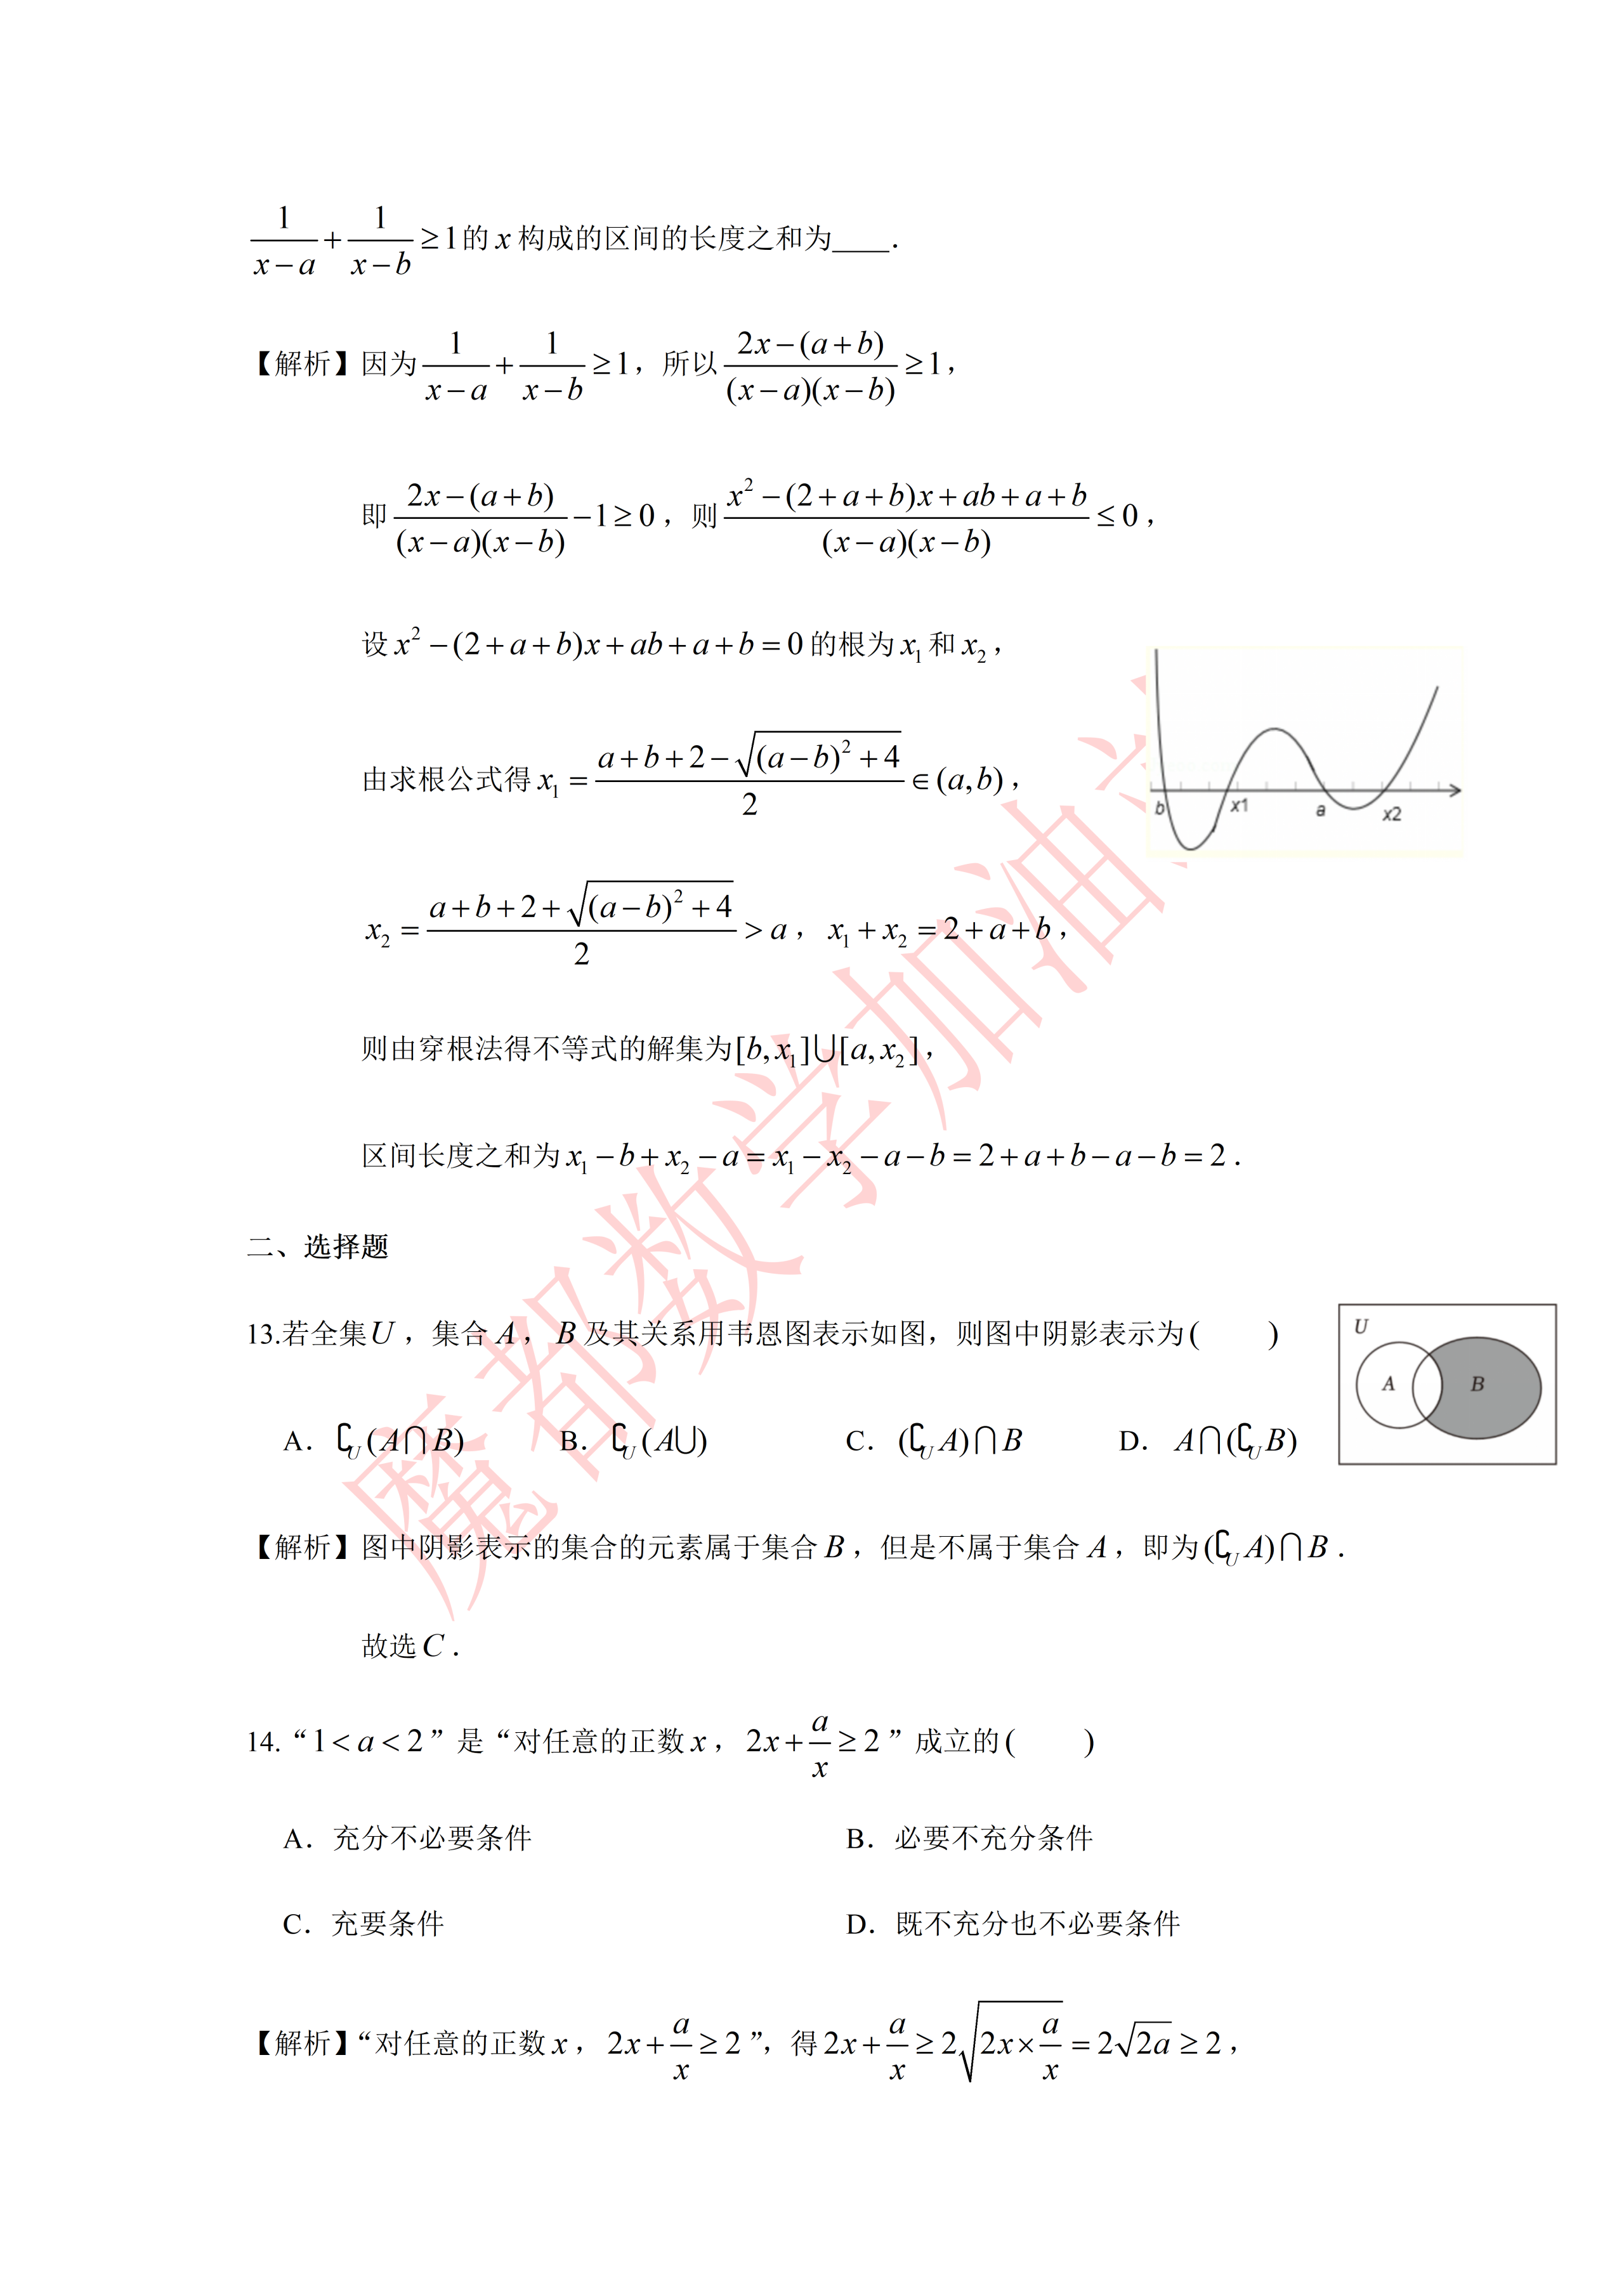
\includegraphics[width=.50\linewidth,trim=1786bp 2255bp 228bp 985bp,clip]{../原图/高一51_华师大二附中_国庆作业3/04.png}
\end{center}
\step{由求根公式得 $x_1=\dfrac{a+b+2-\sqrt{(a-b)^2+4}}{2}\in(a,b)$，}
\step{$x_2=\dfrac{a+b+2+\sqrt{(a-b)^2+4}}{2}>a$，$x_1+x_2=2+a+b$，}
\step{则由穿根法得不等式的解集为 $[b,x_1]\cup[a,x_2]$，}
% 原卷如此，照录未改（此处原卷作 $x_1-x_2$，按上一行 $x_1+x_2=2+a+b$ 当为 $x_1+x_2$）
\step{区间长度之和为 $x_1-b+x_2-a=x_1-x_2-a-b=2+a+b-a-b=2$.}
\solend

\fi

\end{enumerate}

\bigsec{二、选择题}

\begin{enumerate}
\setcounter{enumi}{12}

% 本题是“题干 + 图 + 选项”约 5.5cm 的一整块，图夹在题干与选项之间时 \keepwithprev 挡不住断点，
% 故按 高一30 第 13 题的成例在题前先量一次页高（守卫放在 \item 之前）。
\needvspace{6cm}
\item 若全集 $U$，集合 $A$、$B$ 及其关系用韦恩图表示如图，则图中阴影表示为\mbox{（\quad）}

\begin{center}
% 原卷该图印在题干与选项右侧（原图第 04 页），本稿移作居中排，直接裁取原图，不另存图片文件。
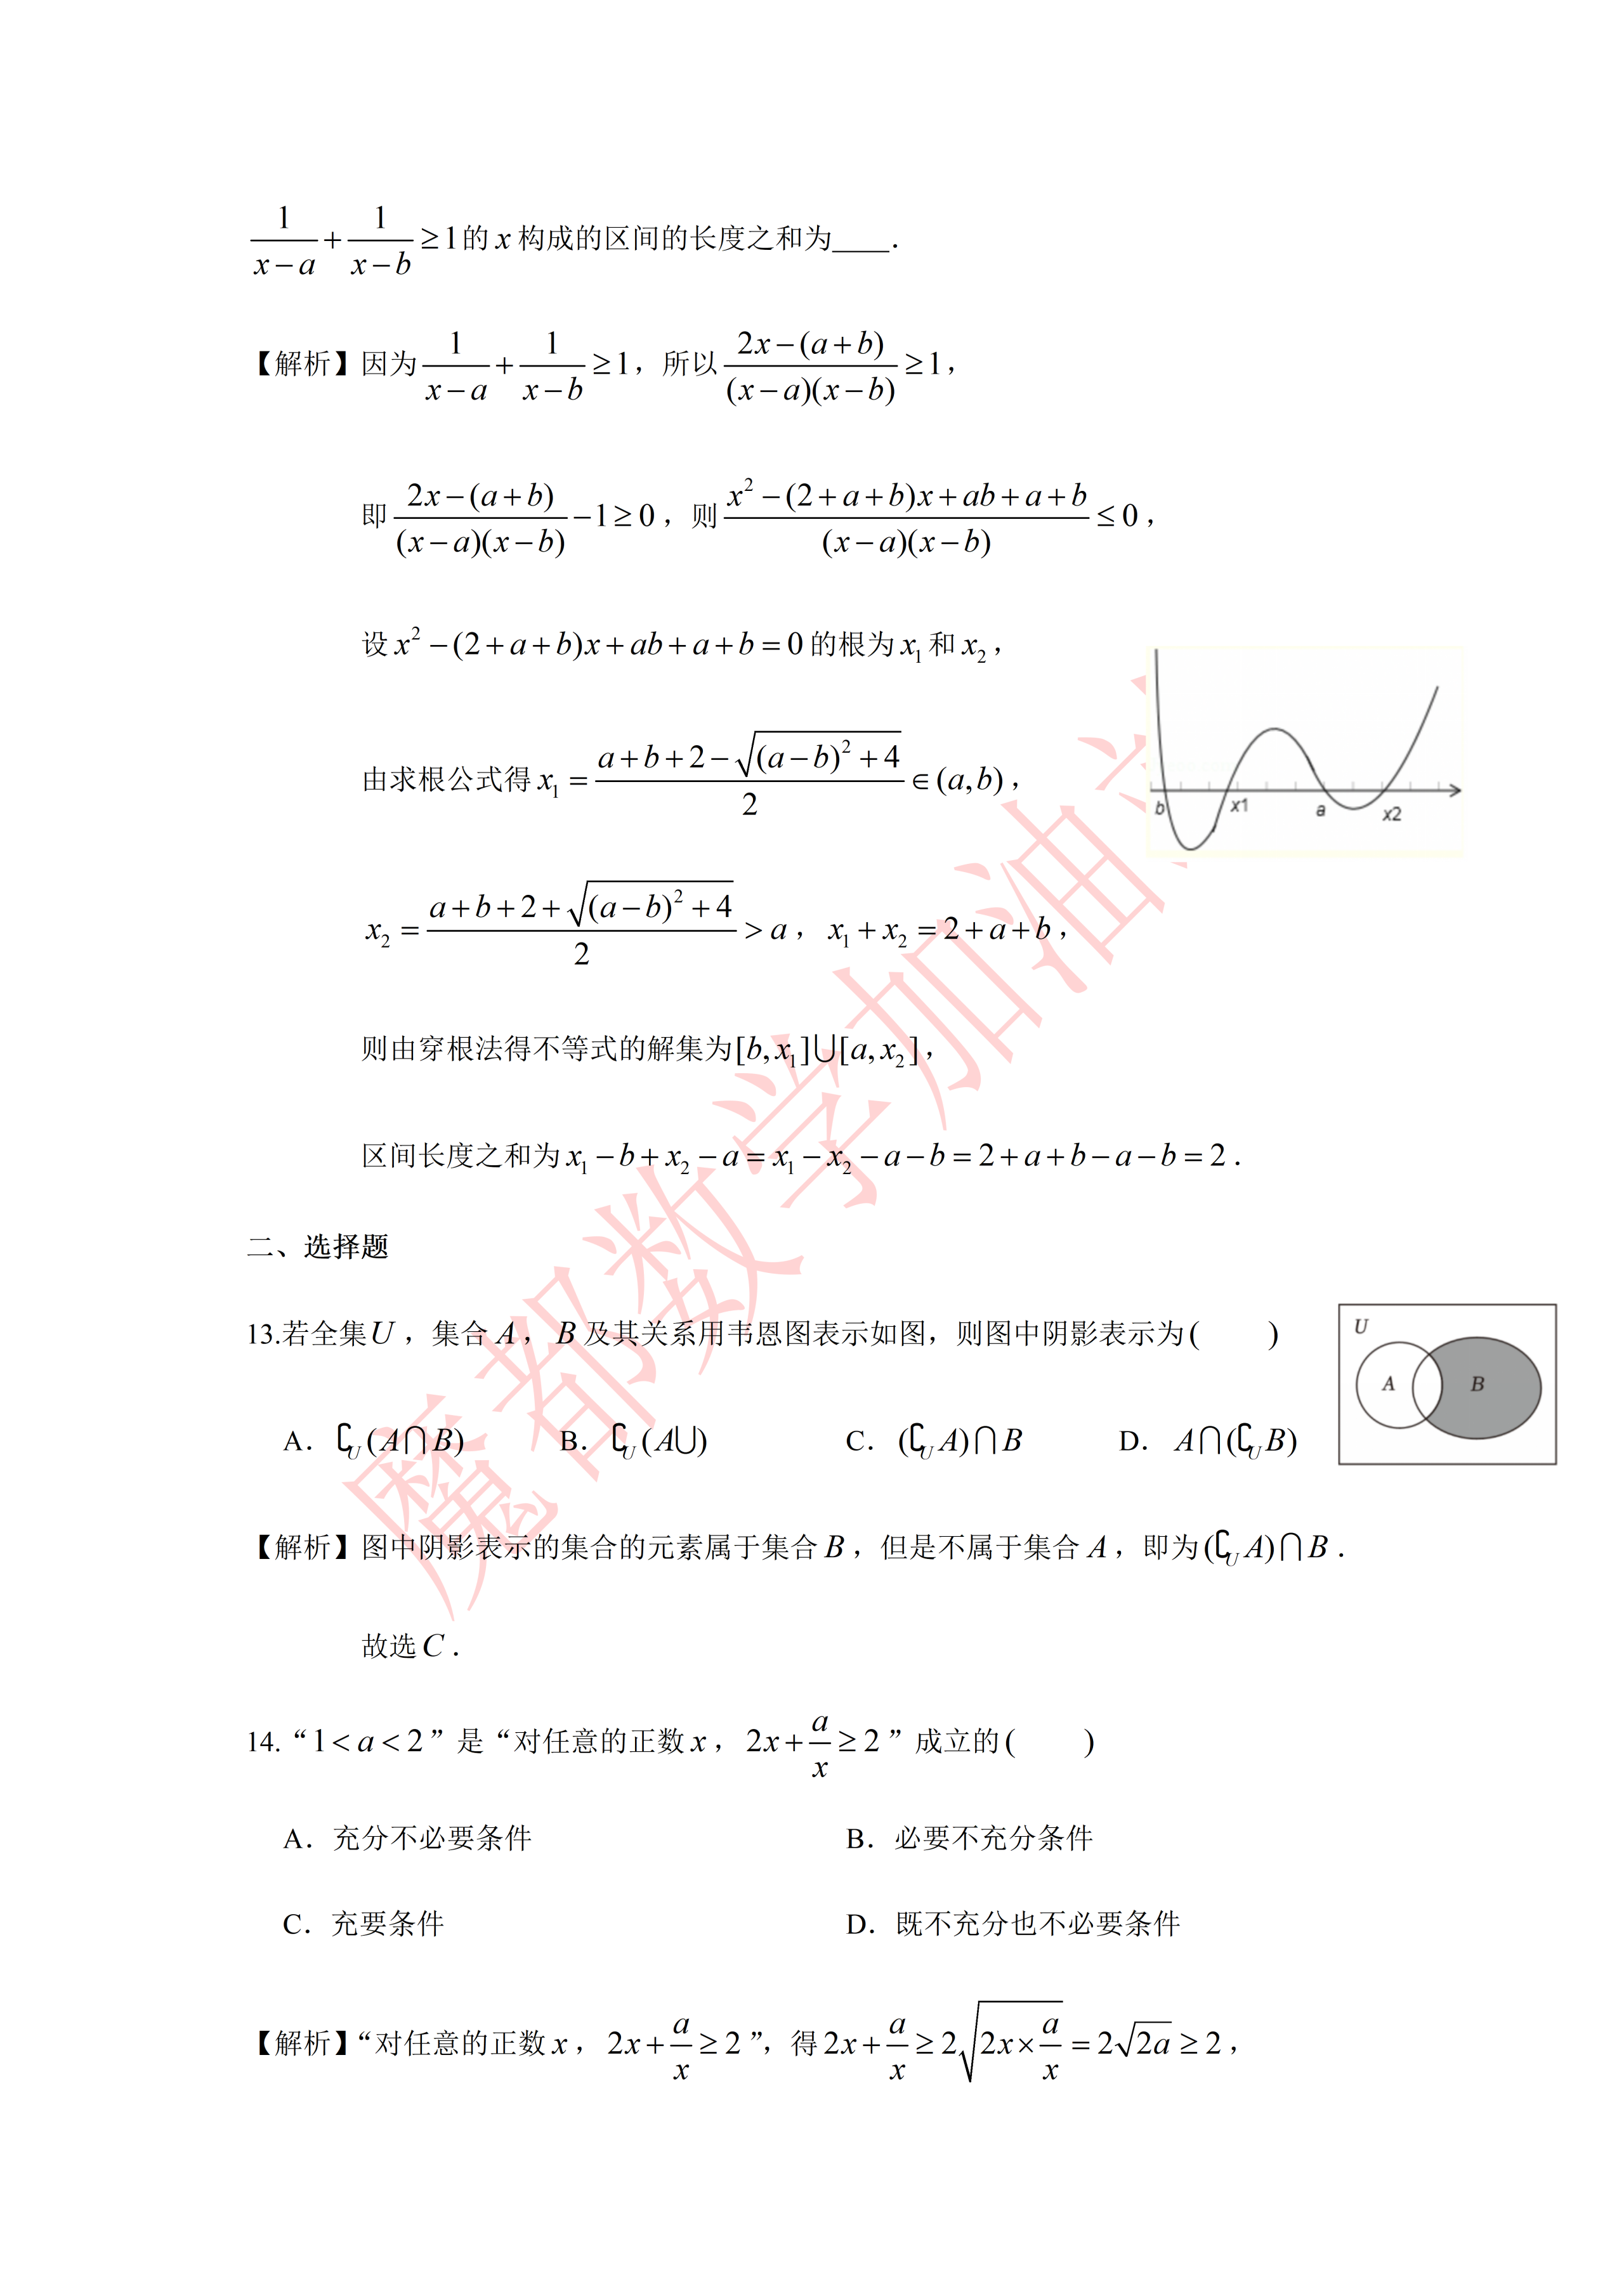
\includegraphics[width=.30\linewidth,trim=2105bp 1308bp 105bp 2050bp,clip]{../原图/高一51_华师大二附中_国庆作业3/04.png}
\end{center}

\keepwithprev
A. $\complement_U(A\cap B)$\qquad B. $\complement_U(A\cup B)$

C. $(\complement_U A)\cap B$\qquad D. $A\cap(\complement_U B)$

\ifanswer
\solbegin
\step{图中阴影表示的集合的元素属于集合 $B$，但是不属于集合 $A$，即为 $(\complement_U A)\cap B$.}
\step{故选 $C$.}
\solend

\fi

\item “$1<a<2$”是“对任意的正数 $x$，$2x+\dfrac ax\geqslant2$”成立的\mbox{（\quad）}

\keepwithprev
A. 充分不必要条件\qquad B. 必要不充分条件

C. 充要条件\qquad\qquad D. 既不充分也不必要条件

\ifanswer
\solbegin
\step{“对任意的正数 $x$，$2x+\dfrac ax\geqslant2$”，得 $2x+\dfrac ax\geqslant2\sqrt{2x\times\dfrac ax}=2\sqrt{2a}\geqslant2$，}
\step{所以 $\sqrt{2a}\geqslant1$，解得 $a\geqslant\dfrac12$，}
\step{若“$1<a<2$”得 $2x+\dfrac ax\geqslant2\sqrt{2x\times\dfrac ax}=2\sqrt{2a}>2\sqrt2>2$，}
\step{所以“$1<a<2$”$\Rightarrow$“对任意的正数 $x$，$2x+\dfrac ax\geqslant2$”，}
\step{所以“$1<a<2$”是“对任意的正数 $x$，$2x+\dfrac ax\geqslant2$”成立的充分不必要条件，}
\step{故选 $A$.}
\solend

\fi

\item 已知函数 $f(x)=2x-3$，$x\in(0,2)$，实数 $a$、$b$ 满足 $f(a)+f(b-1)=0$，则以下成立的有\mbox{（\quad）}

\keepwithprev
A. $a(b-1)$ 的最大值为 $\dfrac94$\qquad\qquad B. $b-\dfrac1a$ 的最大值为 $2$

C. $\dfrac1a+\dfrac1{4b}$ 的最小值为 $\dfrac9{16}$\qquad D. $-1<b-a<3$

\ifanswer
\solbegin
\step{因为函数 $f(x)=2x-3$，$x\in(0,2)$，实数 $a$、$b$ 满足 $f(a)+f(b-1)=0$，}
\step{所以 $2a-3+2(b-1)-3=0$，得 $a+b=4$，$a\in(0,2)$，$b\in(1,3)$，}
\step{所以 $a(b-1)=a(3-a)=-\left(a-\dfrac32\right)^2+\dfrac94$，$a\in(0,2)$，}
\step{所以 $0<a(b-1)\leqslant\dfrac94$，故选项 $A$ 正确；}
\step{$b-\dfrac1a=4-a-\dfrac1a=4-\left(a+\dfrac1a\right)\leqslant4-2=2$，}
\step{当且仅当 $a=1$，$b=3$ 时取等号，又 $b\in(1,3)$，故 $b-\dfrac1a<2$，故 $B$ 错误；}
\step{$\dfrac1a+\dfrac1{4b}=\dfrac14\left(\dfrac1a+\dfrac1{4b}\right)(a+b)=\dfrac14\left(1+\dfrac14+\dfrac ba+\dfrac a{4b}\right)=\dfrac5{16}+\dfrac14\left(\dfrac ba+\dfrac a{4b}\right)$}
\step{$\geqslant\dfrac5{16}+\dfrac14\cdot2\sqrt{\dfrac ba\cdot\dfrac a{4b}}=\dfrac9{16}$，当且仅当 $\dfrac ba=\dfrac a{4b}$，即 $a=2b=\dfrac83$ 时取等号，}
% 原卷如此，照录未改（“又 $a\in(0,2)$，”与下式之间原卷正文夹印“水印”二字）
\step{又 $a\in(0,2)$，水印 $\dfrac1a+\dfrac1{4b}<\dfrac9{16}$，故 $C$ 错误；}
\step{因为 $a\in(0,2)$，$b\in(1,3)$，所以 $-a\in(-2,0)$，所以 $b-a\in(-1,3)$，}
\step{故 $D$ 正确；}
\step{故选 $AD$.}
\solend

\fi

% 本题解析含图（“函数 f(x) 的图像如下”），图夹在解析行间，页末放不下会被拆开，
% 故在题前先量一次页高；上界取“题干 + 选项 + 图 + 首行解析”一块的高度。
\needvspace{6cm}
\item 设 $M_I$ 表示函数 $f(x)=|x^2-4x+2|$ 在闭区间 $I$ 上的最大值. 若正实数 $a$ 满足
$M_{[0,a]}\geqslant2M_{[a,2a]}$，则正实数 $a$ 的取值范围是\mbox{（\quad）}

\keepwithprev
A. $\left[2-\sqrt3,\dfrac12\right]$\qquad B. $[2-\sqrt3,1]$

C. $[2,2+\sqrt3]$\qquad\qquad D. $[2+\sqrt3,4]$

\ifanswer
\solbegin
\step{函数 $f(x)$ 的图像如下：}
\begin{center}
% 原卷该图印在解析行间（原图第 06 页），本稿直接裁取原图，不另存图片文件。
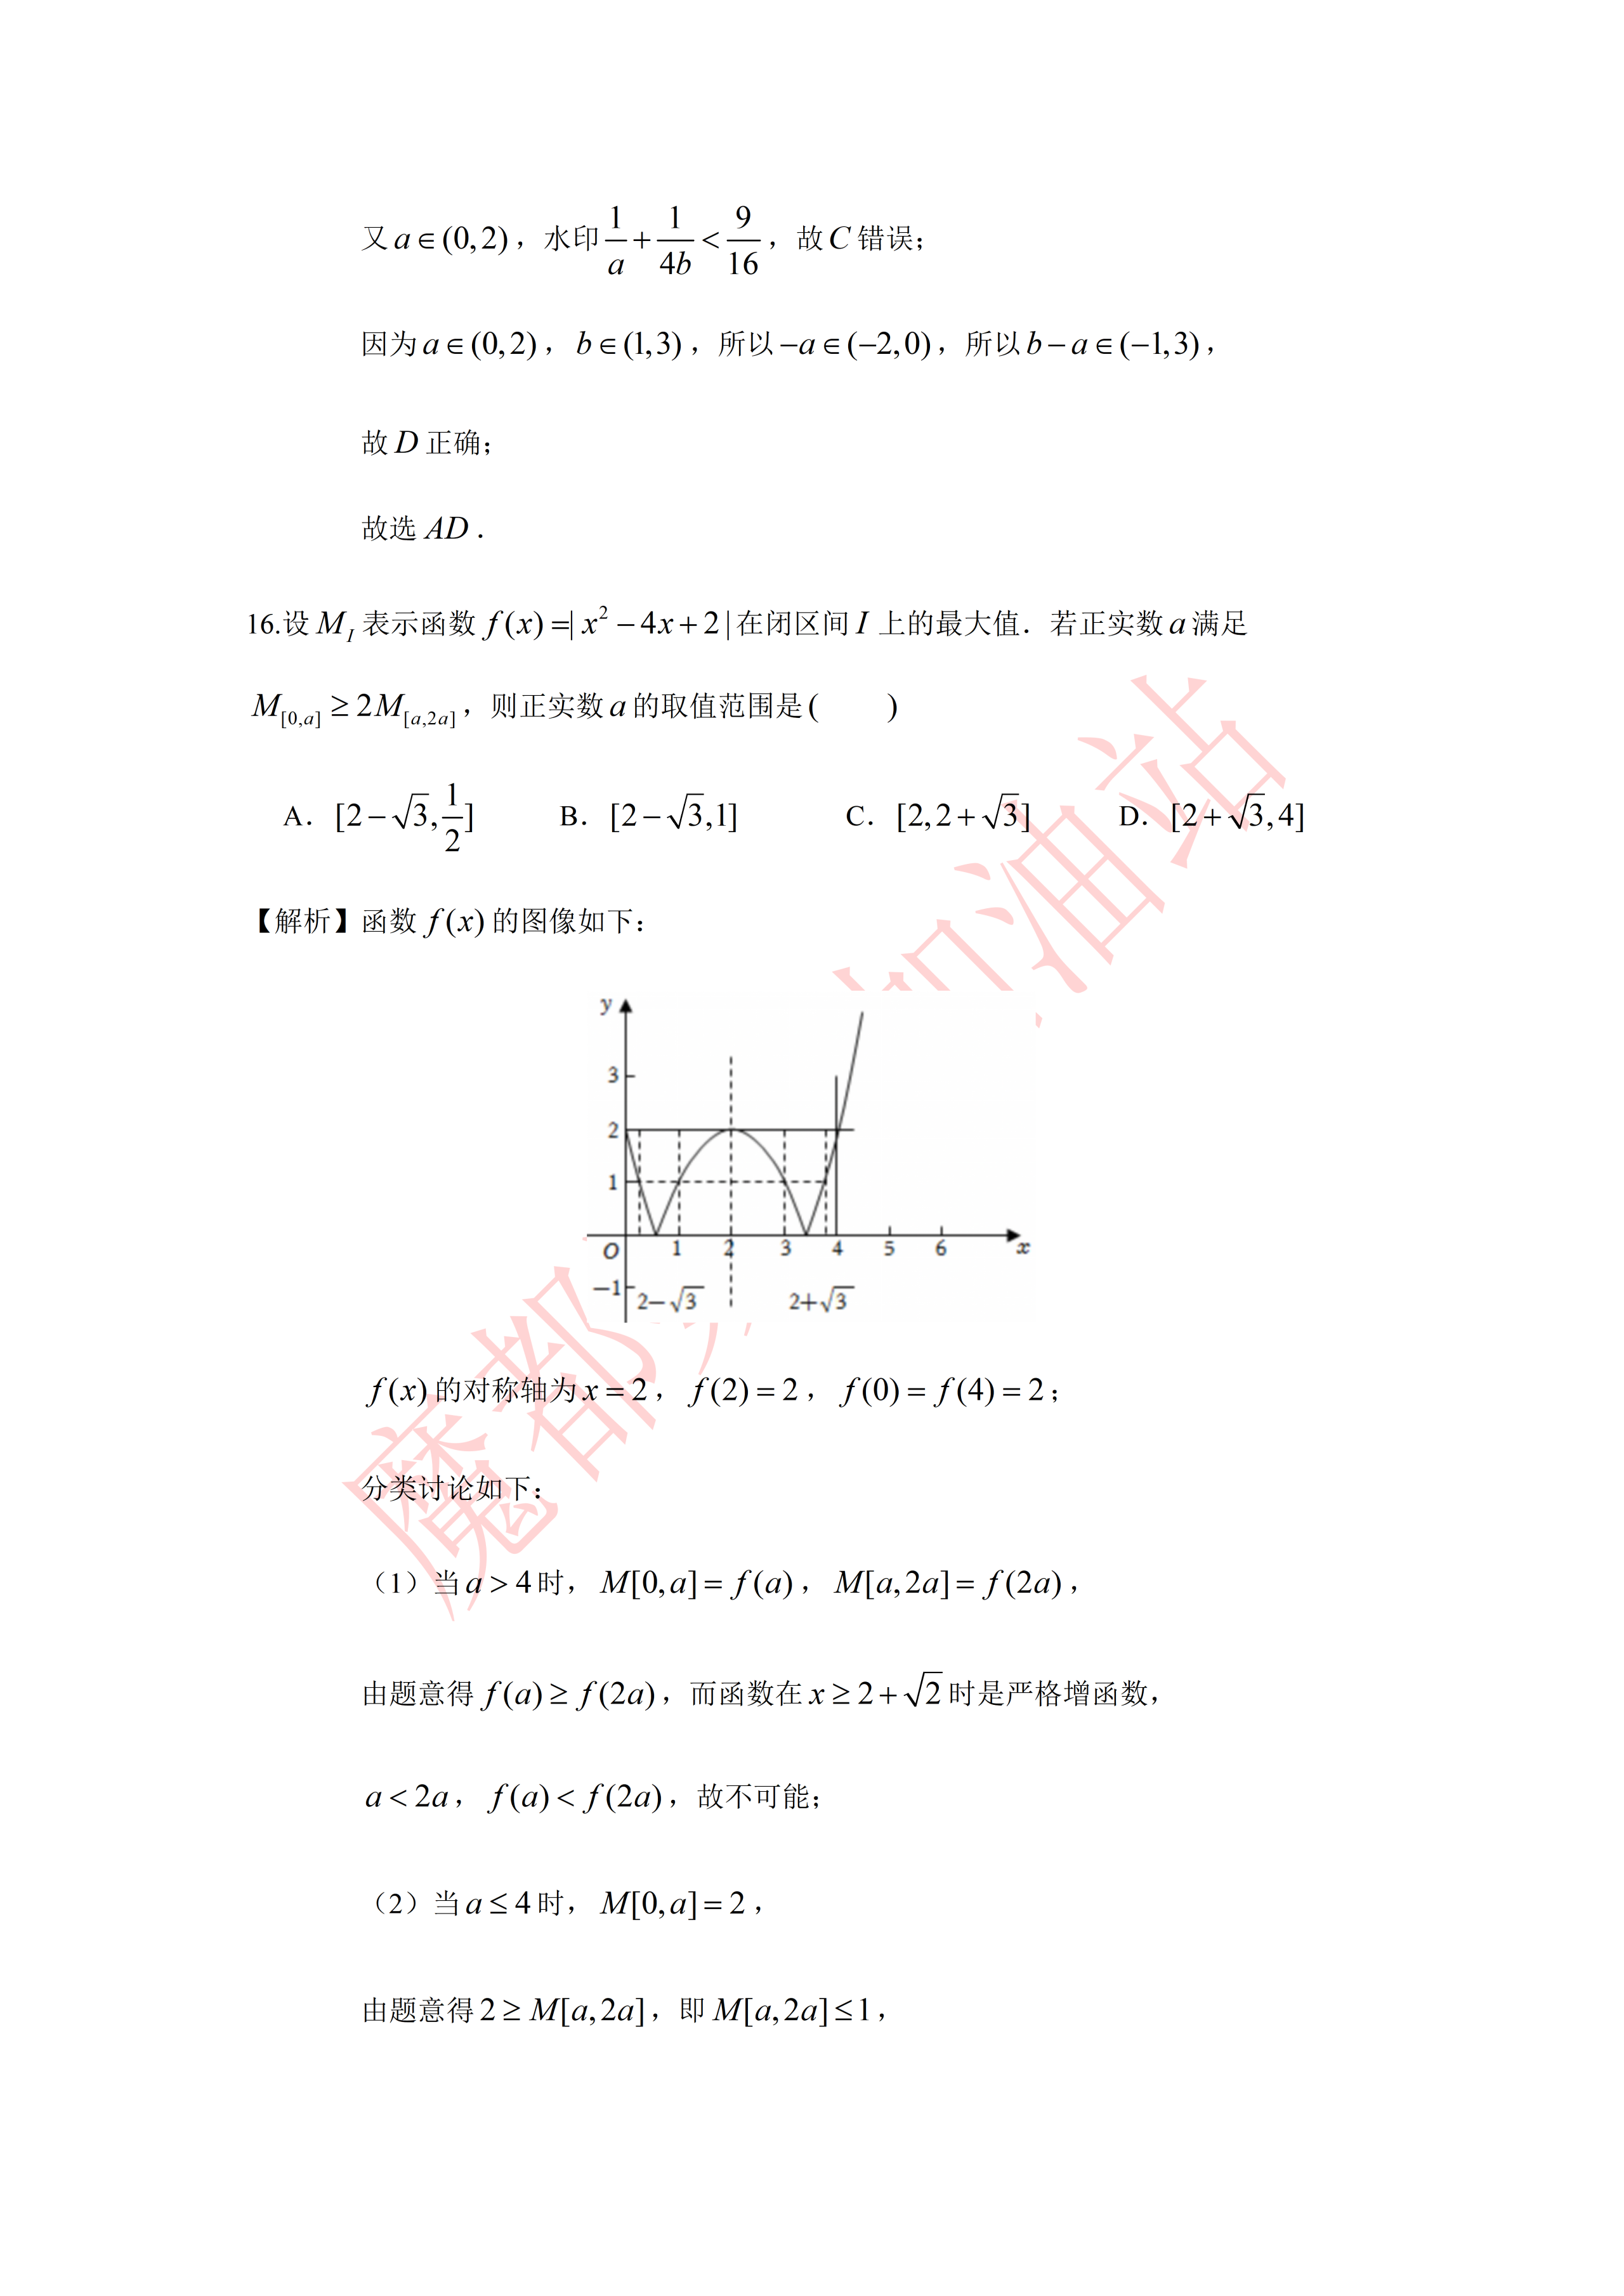
\includegraphics[width=.55\linewidth,trim=895bp 1535bp 915bp 1525bp,clip]{../原图/高一51_华师大二附中_国庆作业3/06.png}
\end{center}
\step{$f(x)$ 的对称轴为 $x=2$，$f(2)=2$，$f(0)=f(4)=2$；}
\step{分类讨论如下：}
\stepm{(1)}{当 $a>4$ 时，$M_{[0,a]}=f(a)$，$M_{[a,2a]}=f(2a)$，}
\step{由题意得 $f(a)\geqslant f(2a)$，而函数在 $x\geqslant2+\sqrt2$ 时是严格增函数，}
\step{$a<2a$，$f(a)<f(2a)$，故不可能；}
\stepm{(2)}{当 $a\leqslant4$ 时，$M_{[0,a]}=2$，}
\step{由题意得 $2\geqslant M_{[a,2a]}$，即 $M_{[a,2a]}\leqslant1$，}
\step{令 $f(x)=1$，解得 $x_1=2-\sqrt3$，$x_2=1$，$x_3=2+\sqrt3$，$x_4=3$，}
\step{则有 $a\geqslant2-\sqrt3$ 并且 $2a\leqslant1$，解得 $2-\sqrt3\leqslant a\leqslant\dfrac12$；}
\step{或者 $a\geqslant3$ 并且 $2a\leqslant2+\sqrt3$，无解；}
\step{故选 $A$.}
\solend

\fi

\end{enumerate}

\bigsec{三、解答题}

\begin{enumerate}
\setcounter{enumi}{16}

\item 已知 $M=\{x\mid2\leqslant x\leqslant5\}$，$N=\{x\mid a-1\leqslant x\leqslant2a+1\}$.
\begin{enumerate}[label=(\arabic*)]
\item 若 $M\subseteq N$，求实数 $a$ 的取值范围；
\item 若 $M\supseteq N$，求实数 $a$ 的取值范围.
\end{enumerate}

\ifanswer
\ans{（1）$[2,3]$；（2）$(-\infty,-2)$}
\fi

\ansspace[6]

\item 设集合 $A=\{x\mid|x+1|\leqslant3\}$，$B=\{x\mid0<x<3m\}$.
\begin{enumerate}[label=(\arabic*)]
\item 若 $A\cup B=A$，求实数 $m$ 的取值范围；
\item 设 $P=(\complement_R A)\cap B$，若 $\exists x\in\Z$ 且 $x\in P$，求实数 $m$ 的取值范围.
\end{enumerate}

\ifanswer
\solbegin
\stepm{(1)}{$A=\{x\mid|x+1|\leqslant3\}=\{x\mid-4\leqslant x\leqslant2\}$，且 $A\cup B=A$，所以 $B\subseteq A$.}
\step{若 $B=\varnothing$，此时 $0\geqslant3m$，解得 $m\leqslant0$；}
\step{若 $B\neq\varnothing$，此时 $0<3m$，且 $3m\leqslant2$，解得 $0<m\leqslant\dfrac23$；}
\step{则实数 $m$ 的取值范围是 $\left(-\infty,\dfrac23\right]$.}
\stepm{(2)}{因为 $\exists x\in\Z$ 且 $x\in P$，所以集合 $P$ 中至少存在一个整数.}
\step{$\complement_R A=\{x\mid x<-4\text{ 或 }x>2\}$，$B=\{x\mid0<x<3m\}$，}
\step{要使 $P=(\complement_R A)\cap B$ 中至少存在一个整数，则 $\begin{cases}3m>0\\3m>3\end{cases}$，解得 $m>1$，}
\step{则实数 $m$ 的取值范围是 $(1,+\infty)$.}
\solend

\fi

\ansspace[7]

\item 已知函数 $f(x)=x^2+(1-a)x-a(a\in\R)$.
\begin{enumerate}[label=(\arabic*)]
\item 解关于 $x$ 的不等式 $f(x)<0$；
\item 若 $\forall a\in[-1,1]$，$f(x)\geqslant0$ 恒成立，求实数 $x$ 的取值范围.
\end{enumerate}

\ifanswer
\solbegin
\stepm{(1)}{不等式 $x^2+(1-a)x-a<0$ 等价于 $(x-a)(x+1)<0$，}
\step{当 $a<-1$ 时，不等式的解集为 $(a,-1)$；}
\step{当 $a=-1$ 时，不等式的解集为 $\varnothing$；}
\step{当 $a>-1$ 时，不等式的解集为 $(-1,a)$.}
\stepm{(2)}{$x^2+(1-a)x-a=-a(x+1)+x^2+x$，}
\step{设 $g(a)=-a(x+1)+x^2+x$，$a\in[-1,1]$，}
\step{要使 $g(a)\geqslant0$ 在 $a\in[-1,1]$ 上恒成立，}
\step{只需 $\begin{cases}g(-1)\geqslant0\\g(1)\geqslant0\end{cases}$，即 $\begin{cases}x^2+2x+1\geqslant0\\x^2-1\geqslant0\end{cases}$，解得 $x\geqslant1$ 或 $x\leqslant-1$，}
\step{所以 $x$ 的取值范围为 $\{x\mid x\leqslant-1\text{ 或 }x\geqslant1\}$.}
\solend

\fi

\ansspace[7]

\item 若实数 $x$、$y$、$m$ 满足 $|x-m|>|y-m|$，则称 $x$ 比 $y$ 远离 $m$.
\begin{enumerate}[label=(\arabic*)]
\item 若 $2$ 比 $3x-4$ 远离 $1$，求 $x$ 的取值范围；
\item 设 $y=\dfrac{x+2}{x+1}$，其中 $x\in(0,\sqrt2)\cup(\sqrt2,+\infty)$，判断：$x$ 与 $y$ 哪一个更远离 $\sqrt2$？并说明理由.
\item 若 $x+y=2$，试问：$y$ 与 $x^2+y^2$ 哪一个更远离 $\dfrac12$？并说明理由.
\end{enumerate}

\ifanswer
\solbegin
\stepm{(1)}{由题意得 $|2-1|>|3x-4-1|$，所以 $|3x-5|<1$，解得 $\dfrac43<x<2$，}
\step{故 $x$ 的取值范围为 $\left(\dfrac43,2\right)$；}
\stepm{(2)}{$x$ 比 $y$ 更远离 $\sqrt2$，}
\step{理由如下：要证 $x$ 比 $y$ 更远离 $\sqrt2$，只要证 $|x-\sqrt2|>\left|\dfrac{x+2}{x+1}-\sqrt2\right|$，}
\step{即证 $|x-\sqrt2|>\left|\dfrac{(1-\sqrt2)(x-\sqrt2)}{x+1}\right|$，}
\step{因为 $x\in(0,\sqrt2)\cup(\sqrt2,+\infty)$，所以 $|x-\sqrt2|>0$，}
\step{所以只要证 $1>\dfrac{\sqrt2-1}{|x+1|}$，即证 $|x+1|>\sqrt2-1$，}
\step{因为 $x\in(0,\sqrt2)\cup(\sqrt2,+\infty)$，所以 $x+1\in(1,\sqrt2+1)\cup(\sqrt2+1,+\infty)$，}
\step{所以 $|x+1|>1>\sqrt2-1$，所以 $x$ 比 $y$ 更远离 $\sqrt2$；}
\stepm{(3)}{因为 $x^2+y^2\geqslant\dfrac{(x+y)^2}{2}=2$，当且仅当 $x=y=1$ 时等号成立，}
\step{所以 $\left|x^2+y^2-\dfrac12\right|=x^2+y^2-\dfrac12$，}
\step{从而 $\left|y-\dfrac12\right|-\left|x^2+y^2-\dfrac12\right|=\left|y-\dfrac12\right|-\left(x^2+y^2-\dfrac12\right)$，}
\step{①$y\geqslant\dfrac12$，$\left|y-\dfrac12\right|-\left|x^2+y^2-\dfrac12\right|=y-\dfrac12-\left(x^2+y^2-\dfrac12\right)=y-x^2-y^2$}
\step{$=y-(2-y)^2-y^2=-2y^2+5y-4=-2\left(y-\dfrac54\right)^2-\dfrac78<0$，}
\step{即 $\left|y-\dfrac12\right|<\left|x^2+y^2-\dfrac12\right|$；}
\step{②$y<\dfrac12$，}
\step{$\left|y-\dfrac12\right|-\left|x^2+y^2-\dfrac12\right|=\left(\dfrac12-y\right)-\left(x^2+y^2-\dfrac12\right)=-y-x^2-y^2+1$}
\step{$=-y-(2-y)^2-y^2+1=-2y^2+3y-3=-2\left(y-\dfrac34\right)^2-\dfrac{15}8<0$，}
\step{即 $\left|y-\dfrac12\right|<\left|x^2+y^2-\dfrac12\right|$；}
\step{综上，$\left|y-\dfrac12\right|<\left|x^2+y^2-\dfrac12\right|$，即 $x^2+y^2$ 比 $y$ 更远离 $\dfrac12$.}
\solend

\fi

\ansspace[9]

\item 对于非空有限整数集 $X$，$m\in\N^*$，定义 $X^m=\{x^m\mid x\in X\}$，对 $n\in\Z$，
$Y\oplus n=\{x+n\mid x\in Y\}$ 现有两个非空有限整数集 $A$、$B$，已知 $A\oplus1\subseteq B$ 且
$B^2\oplus(-4)\subseteq A$.
\begin{enumerate}[label=(\arabic*)]
\item 当 $A=\{-3,0\}$ 时求集合 $B$；
\item 证明：$A\subseteq\{-3,-2,0,1\}$；
\item 当 $A\oplus1=B$ 且 $B^2\oplus(-4)=A$ 时，任取 $a\in A$，$b\in B$ 构造函数
$f(x)=(x-a)(x-b)$ 问：当 $a$、$b$ 取何值时，$f(x)$ 的最小值最小？
\end{enumerate}

\ifanswer
\solbegin
\stepm{(1)}{因为 $A=\{-3,0\}$，$B^2\oplus(-4)\subseteq A$，}
\step{所以 $B^2\oplus(-4)$ 可能为 $\varnothing$、$\{-3\}$、$\{0\}$、$\{-3,0\}$，}
\step{当 $B^2\oplus(-4)=\varnothing$ 时 $B^2=\varnothing$，不满足非空，不合题意；}
\step{当 $B^2\oplus(-4)=\{-3\}$ 时 $B^2=\{1\}$，所以 $B=\{1,-1\}$、$\{1\}$、$\{-1\}$，}
\step{当 $B^2\oplus(-4)=\{0\}$ 时 $B^2=\{4\}$，所以 $B=\{2,-2\}$、$\{2\}$、$\{-2\}$，}
% 原卷如此，照录未改（此处作 $\{0,-3\}$，上一行同一集合作 $\{-3,0\}$）
\step{当 $B^2\oplus(-4)=\{0,-3\}$ 时 $B^2=\{4,1\}$，}
\step{所以 $B=\{1,2,-1,-2\}$、$\{2,-1,-2\}$、$\{2,1,-2\}$、$\{1,-1,-2\}$、$\{1,-1,2\}$、$\{1,2\}$、$\{-1,2\}$、$\{-1,-2\}$、$\{1,-2\}$，}
\step{又 $A\oplus1=\{-2,1\}\subseteq B$，得 $B$ 为 $\{1,-2\}$、$\{2,1,-2\}$、$\{1,-1,-2\}$、$\{1,2,-1,-2\}$.}
\stepm{(2)}{设 $x\in A$，因为 $A\oplus1\subseteq B$，所以 $x+1\in B$，}
\step{又 $B^2\oplus(-4)\subseteq A$，所以 $(x+1)^2-4\in A$，}
% 原卷如此，照录未改（此处及下文取 $x=2$ 处原卷均作 $(-4+1)^2-4=52-2a>0$）
\step{取 $x=-4$，则 $(-4+1)^2-4=52-2a>0$，$(5+1)^2-4=32\in A$，$\cdots$，}
\step{无限迭代，而 $A$ 为有限集，不合题意，舍去，即 $-4\notin A$；}
\step{取 $x=-3$，则 $(-3+1)^2-4=0\in A$，$(0+1)^2-4=-3\in A$，}
\step{得 $A$ 集合可为 $\{-3,0\}$；}
\step{取 $x=-2$，则 $(-2+1)^2-4=-3\in A$，$(-3+1)^2-4=0\in A$，}
\step{$(0+1)^2-4=-3\in A$，得 $A$ 集合可为 $\{-3,-2,0\}$；}
\step{取 $x=-1$，则 $(-1+1)^2-4=-4\in A$，又 $-4\notin A$，所以 $-1\notin A$，}
\step{取 $x=1$，则 $(1+1)^2-4=0\in A$，$(0+1)^2-4=-3\in A$，}
\step{$(-3+1)^2-4=0\in A$，得 $A$ 集合可为 $\{-3,0,1\}$，}
\step{取 $x=2$，则 $(2+1)^2-4=52-2a>0$，$(5+1)^2-4=32\in A$，$\cdots$，}
\step{无限迭代，而 $A$ 为有限集，不合题意，舍去，即 $2\notin A$，}
\step{同理当 $x<-4$ 或 $x>2$，且 $x\in\Z$ 时不符合 $A$ 为有限集，舍去；}
\step{故由上得 $A$ 集合可为 $\{-3,0\},\{-3,-2,0\},\{-3,0,1\},\{-3,-2,0,1\}$，}
\step{所以 $A\subseteq\{-3,-2,0,1\}$，}
\stepm{(3)}{当 $A\oplus1=B$ 且 $B^2\oplus(-4)=A$ 时，}
\step{设 $x\in B$，则 $x^2-4\in B^2\oplus(-4)=A$，}
% 原卷如此，照录未改（题设 $A=\{-3,0\}$，此处两个判别式取的是 $-2$ 与 $1$，均不属于 $A$）
\step{$x^2-4=-2$ 时 $x=\pm\sqrt2$，不为整数，不合题意；}
\step{$x^2-4=1$ 时 $x=\pm\sqrt5$，不为整数，不合题意；}
\step{所以 $A=\{-3,0\}$，又 $A\oplus1=B$，则 $B=\{-2,1\}$，}
\step{任取 $a\in A$，$b\in B$ 构造函数 $f(x)=(x-a)(x-b)$，}
\step{$f(x)=(x-a)(x-b)=x^2-(a+b)x+ab$}
\step{$=x^2-(a+b)x+\dfrac{(a+b)^2}{4}+ab-\dfrac{(a+b)^2}{4}$}
\step{$=\left[x-\dfrac{(a+b)}2\right]^2-\dfrac{(a-b)^2}{4}\geqslant-\dfrac{(a-b)^2}{4}$，所以 $f(x)_{min}=-\dfrac{(a-b)^2}{4}$，}
\step{又 $a\in A=\{-3,0\}$，$b\in B=\{-2,1\}$，所以 $a-b$ 的取值有 $-1,-4,2$，}
\step{所以 $f(x)_{min}=-\dfrac{(a-b)^2}{4}\geqslant-\dfrac{(-3-1)^2}{4}=-4$，}
\step{即当 $a=-3$，$b=1$ 时 $f(x)_{min}$ 的最小值为 $-4$.}
\solend

\fi

\ansspace*[12]

\end{enumerate}

\end{document}
"
% 紧凑版：xelatex "\def\iscompact{1}% 高一51_华师大二附中_国庆作业3.tex
%   —— 高一上数学“2026-2027 年华师大二附中高一上国庆作业 3”（讲评版）
% 试卷版：xelatex 高一51_华师大二附中_国庆作业3.tex
% 答案版：xelatex "\def\isanswer{1}\input{高一51_华师大二附中_国庆作业3.tex}"
% 紧凑版：xelatex "\def\iscompact{1}\input{高一51_华师大二附中_国庆作业3.tex}"
%
% 原始材料：微信公众号“魔都数学加油站”文章，作者破晓，连载“27学年高一51”；
% 原文标题“27学年高一51——2026-2027年上海市华师大二附中高一上国庆作业3”；
% 原文链接：https://mp.weixin.qq.com/s/95SLMEmPUT30s4U7wjr5Og。
% 该页面用 JS 渲染，未见明确发布日期；页面内时间戳约为 2026-10-05 21:37，本稿以该时刻记可得日期。
% 正文为 12 张 PNG 页：第 01、02、03、05、07、08、11 页 4762×6735，
% 第 04、06、09、10、12 页 2560×3620。按页序逐页读取，12 页全为试卷正文页
% （卷首标题在第 1 页页顶，卷末解答题止于第 12 页），无封面页、目录页或单独的页脚页。
% 卷面标题照原卷印作“2026-2027 年华师大二附中高一上国庆作业 3”（公众号标题中的“上海市”
% 卷面标题行没有，本稿照卷面），年份区间按全稿惯例排 en dash。
%
% 篇幅与题号：原卷自第 3 题起编号（第 1、2 题不在本卷内）。填空题 3—12（10 题）、
% 选择题 13—16（4 题）、解答题 17—21（5 题），共 19 题。本稿沿用原节与原题号，
% 只改排为全稿统一的大节样式（原卷小节标题为“一、填空题”“二、选择题”“三、解答题”）。
% 正文为讲评版：填空题 3—12 与选择题 13—16 只印【解析】（选择题的结论“故选 X”印在解析内），
% 按全稿口径这类题不另提 \ans{}；解答题第 17 题只印【答案】，故只给 \ans{}；
% 第 18—21 题只印【解析】。
%
% 副标题：原卷未印副标题。本稿按“知识模块”口径标作“集合与常用逻辑用语、不等式”：
% 19 题中集合与常用逻辑用语 8 题（3、4、6、10、13、17、18、21），
% 不等式（含函数最值、绝对值不等式）11 题（5、7、8、9、11、12、14、15、16、19、20），
% 两类均远超三分之一，故并标。口径同 高一46_交附闵行_国庆作业3、高一48_华师大二附中_周末作业2。
%
% 与原卷的排版差异：
%   ① 原卷每题下直接印【答案】或【解析】，本稿按全稿惯例将答案与解析置于答案版；
%   ② 原卷未印副标题，本稿按“知识模块”口径补出；
%   ③ 原卷填空横线按全稿惯例排为 \blankline[4.4em]；
%   ④ 原卷 $R$、$N$、$Z$ 均排斜体，本稿按全稿惯例改用花体 $\R$、$\N$、$\Z$（同 高一48）；
%   ⑤ 原卷第 12 题解析配图、第 13 题题干韦恩图都印在正文右侧的浮动位置，第 16 题解析配图
%      印在解析行间；本稿三图一律居中排，均自原图对应页裁切（trim），不另存图片文件；
%   ⑥ 原卷解答题未留作答空白，本稿按全稿惯例加 \ansspace；
%   ⑦ 原卷第 15 题解析第 7、8 两个印刷行是一串连等式的折行，本稿按“一条 \step ＝ 一个印刷行”
%      的口径分成两条 \step。
%
% 原卷笔误/存疑（均照录未改，正文对应处另有 % 注）：
%   ① 第 12 题解析末行作“区间长度之和为 $x_1-b+x_2-a=x_1-x_2-a-b=2+a+b-a-b=2$”，
%      按上一行 $x_1+x_2=2+a+b$，此处应为 $x_1+x_2$；原卷作 $x_1-x_2$。
%   ② 第 15 题解析“又 $a\in(0,2)$，”与 $\dfrac1a+\dfrac1{4b}<\dfrac9{16}$ 之间，
%      原卷正文夹印“水印”二字（系制版遗留字样，非试卷内容）。
%   ③ 第 21 题第 (2) 问解析两处（取 $x=-4$、取 $x=2$）作“$=52-2a>0$”，
%      与题设 $(x+1)^2-4$ 的取值（按 $x=-4$ 应为 $5$）不符，当系原卷算式遗留。
%   ④ 第 21 题第 (1) 问解析先写 $B^2\oplus(-4)$ 可能为 $\{-3,0\}$，后文又作 $\{0,-3\}$，
%      同一集合两种写法。
%   ⑤ 第 21 题第 (3) 问解析：题设 $B^2\oplus(-4)=A$ 且 $A=\{-3,0\}$ 时，由 $x^2-4\in A$
%      应得 $x^2-4=-3$ 或 $0$；原卷讨论的却是 $x^2-4=-2$ 与 $x^2-4=1$（两值均不属于 $A$），
%      与题设不合。
%
% 插图：3 张，均自原图裁切（无 \begin{tikzpicture} 重排）：
%   · 第 13 题题干韦恩图（原图第 04 页，图在题干与选项右侧）
%   · 第 12 题解析配图（原图第 04 页，图在解析右侧）
%   · 第 16 题解析配图（原图第 06 页，图在解析中间）
%
\documentclass[a4paper,11pt]{article}
\usepackage{common}

\begin{document}

\examtitlest[3]{2026--2027 年华师大二附中高一上国庆作业 3}{集合与常用逻辑用语、不等式}

\bigsec{一、填空题}

\begin{enumerate}
\setcounter{enumi}{2}

\item 若 $\{x\mid x<1\text{ 或 }x>4\}\cup\{x\mid m<x<2m+3\}=R$，则实数 $m$ 的取值范围为\blankline[4.4em].

\ifanswer
\solbegin
\step{因为 $\{x\mid x<1\text{ 或 }x>4\}\cup\{x\mid m<x<2m+3\}=R$，}
\step{所以 $\begin{cases}m<1\\2m+3>4\end{cases}$，解得 $\dfrac12<m<1$，所以 $m$ 的取值范围为 $\left(\dfrac12,1\right)$.}
\solend

\fi

\item 若“$x\leqslant5$”是“$x<a$”的必要不充分条件，则 $a$ 的取值范围是\blankline[4.4em].

\ifanswer
\solbegin
\step{若“$x\leqslant5$”是“$x<a$”的必要不充分条件，则 $\{x\mid x<a\}\subset\{x\mid x\leqslant5\}$，}
\step{所以 $a\leqslant5$.}
\solend

\fi

\item 实数 $x$、$y$ 满足 $x^2+2xy+4y^2=1$，则 $x+2y$ 的取值范围是\blankline[4.4em].

\ifanswer
\solbegin
\step{因为 $x^2+2xy+4y^2=(x+2y)^2-2xy=1$，}
\step{所以 $(x+2y)^2-1=x\cdot(2y)\leqslant\left(\dfrac{x+2y}{2}\right)^2$，当且仅当 $x=2y$ 时取等号，}
\step{解得 $-\dfrac{2\sqrt3}{3}\leqslant x+2y\leqslant\dfrac{2\sqrt3}{3}$，故 $x+2y$ 的取值范围是 $\left[-\dfrac{2\sqrt3}{3},\dfrac{2\sqrt3}{3}\right]$.}
\solend

\fi

\item 若命题 $p$：“$\exists x\in\R$，$5x^2-3x+m=0$”为假命题，则实数 $m$ 的取值范围为\blankline[4.4em].

\ifanswer
\solbegin
\step{若命题 $p$：$\exists x\in\R$，$5x^2-3x+m=0$ 为假命题，}
\step{则 $5x^2-3x+m=0$ 没有实数根，故 $\Delta=9-20m<0$，解得 $m>\dfrac9{20}$.}
\solend

\fi

\item 若当 $3\leqslant m\leqslant5$ 时，$mx^2-mx+m-9<0$ 有解，则实数 $x$ 的取值范围是\blankline[4.4em].

\ifanswer
\solbegin
\step{当 $3\leqslant m\leqslant5$ 时，$mx^2-mx+m-9<0$ 有解，}
\step{即 $(x^2-x+1)m-9<0$ 在 $m\in[3,5]$ 上有解，}
\step{因为 $x^2-x+1>0$，所以一次函数 $g(m)=(x^2-x+1)m-9$ 严格增，}
\step{所以只需 $g(3)=3x^2-3x-6<0$ 即可，}
\step{即 $x^2-x-2<0$，$(x-2)(x+1)<0$，解得 $-1<x<2$，}
\step{所以实数 $x$ 的取值范围是 $(-1,2)$.}
\solend

\fi

\item 已知不等式 $\dfrac{x}{x^2+4}\leqslant a$ 对任意的 $x\in[1,3]$ 恒成立，则实数 $a$ 的范围为\blankline[4.4em].

\ifanswer
\solbegin
\step{因为 $x\in[1,3]$，所以 $\dfrac{x}{x^2+4}=\dfrac{1}{x+\dfrac4x}\leqslant\dfrac{1}{2\sqrt{x\times\dfrac4x}}=\dfrac14$，}
\step{当且仅当 $x=\dfrac4x$ 时，即 $x=2$ 时取等号，即 $\dfrac{x}{x^2+4}$ 在 $x\in[1,3]$ 的最大值为 $\dfrac14$，}
\step{又由不等式 $\dfrac{x}{x^2+4}\leqslant a$ 对任意的 $x\in[1,3]$ 恒成立，所以 $a\geqslant\dfrac14$，}
\step{即实数 $a$ 的范围为 $\left[\dfrac14,+\infty\right)$.}
\solend

\fi

\item 甲、乙两人解关于 $x$ 的不等式 $x^2+bx+c<0$，甲写错了 $b$，正确计算后得到的解为 $\{x\mid1<x<2\}$；
乙写错了 $c$，正确计算后得到的解为 $\{x\mid-4<x<1\}$. 那么不等式 $\dfrac{bx+c}{x-2}<0$ 的解为\blankline[4.4em].

\ifanswer
\solbegin
\step{由 $x^2+bx+c<0$ 的解为 $\{x\mid1<x<2\}$，}
\step{则 $1$ 和 $2$ 是方程 $x^2+bx+c=0$ 的两个根，}
\step{甲写错了 $b$，但 $c$ 是正确的，所以 $c=1\times2=2$；}
\step{由 $x^2+bx+c<0$ 的解为 $\{x\mid-4<x<1\}$，}
\step{则 $-4$ 和 $1$ 是方程 $x^2+bx+c=0$ 的两个根，}
\step{乙写错了 $c$，但 $b$ 是正确的，所以 $-b=-4+1=-3$，即 $b=3$.}
\step{由 $\dfrac{bx+c}{x-2}<0$，得 $\dfrac{3x+2}{x-2}<0$，即 $(3x+2)(x-2)<0$，解得 $-\dfrac23<x<2$.}
\step{不等式 $\dfrac{bx+c}{x-2}<0$ 的解为 $\left\{x\mid-\dfrac23<x<2\right\}$.}
\solend

\fi

\item 已知 $\dfrac{1}{x-2}\geqslant1$ 是 $|x-a|<2$ 的充分非必要条件，则实数 $a$ 的取值范围是\blankline[4.4em].

\ifanswer
\solbegin
\step{由 $\dfrac{1}{x-2}\geqslant1$ 得 $\dfrac{3-x}{x-2}\geqslant0$，解得 $2<x\leqslant3$，由 $|x-a|<2$ 得 $a-2<x<a+2$，}
\step{因为 $\dfrac{1}{x-2}\geqslant1$ 是 $|x-a|<2$ 的充分非必要条件，}
\step{所以 $\{x\mid2<x\leqslant3\}\subset\{x\mid a-2<x<a+2\}$，所以 $\begin{cases}a-2\leqslant2\\a+2>3\end{cases}$，解得 $1<a\leqslant4$，}
\step{即实数 $a$ 的取值范围是 $(1,4]$.}
\solend

\fi

\item 设 $a>0$，$b>0$，若不等式 $a(a+1)^2+b(b+1)^2\geqslant\lambda ab$ 恒成立，则实数 $\lambda$ 的最大值为\blankline[4.4em].

\ifanswer
\solbegin
\step{$a(a+1)^2+b(b+1)^2\geqslant\lambda ab\Leftrightarrow\lambda\leqslant\dfrac{a(a+1)^2+b(b+1)^2}{ab}=\dfrac{(a+1)^2}{b}+\dfrac{(b+1)^2}{a}$，}
\step{从而原问题转化为求 $\dfrac{(a+1)^2}{b}+\dfrac{(b+1)^2}{a}$ 的最小值.}
\step{因为 $\dfrac{(a+1)^2}{b}+\dfrac{(b+1)^2}{a}=\dfrac{b^2+2b+1}{a}+\dfrac{a^2+2a+1}{b}$}
\step{$=\left(\dfrac{b^2}{a}+\dfrac{a^2}{b}\right)+2\left(\dfrac ba+\dfrac ab\right)+\left(\dfrac1a+\dfrac1b\right)\geqslant2\sqrt{\dfrac{b^2}{a}\cdot\dfrac{a^2}{b}}+2\times2\sqrt{\dfrac ba\cdot\dfrac ab}+2\sqrt{\dfrac1a\cdot\dfrac1b}$}
\step{$=2\sqrt{ab}+4+\dfrac{2}{\sqrt{ab}}\geqslant2\sqrt{2\sqrt{ab}\cdot\dfrac{2}{\sqrt{ab}}}+4=8$，以上均当且仅当 $a=b$ 时取等号，}
\step{所以 $\lambda\leqslant8$，即实数 $\lambda$ 的最大值为 $8$.}
\solend

\fi

\item 定义区间 $(a,d)$、$[a,d)$、$(a,d]$、$[a,d]$ 的长度为 $d-a$（$d>a$），已知 $a>b$，则满足
$\dfrac{1}{x-a}+\dfrac{1}{x-b}\geqslant1$ 的 $x$ 构成的区间的长度之和为\blankline[4.4em].

\ifanswer
\solbegin
\step{因为 $\dfrac{1}{x-a}+\dfrac{1}{x-b}\geqslant1$，所以 $\dfrac{2x-(a+b)}{(x-a)(x-b)}\geqslant1$，}
\step{即 $\dfrac{2x-(a+b)}{(x-a)(x-b)}-1\geqslant0$，则 $\dfrac{x^2-(2+a+b)x+ab+a+b}{(x-a)(x-b)}\leqslant0$，}
\step{设 $x^2-(2+a+b)x+ab+a+b=0$ 的根为 $x_1$ 和 $x_2$，}
\begin{center}
% 原卷该图印在解析右侧（原图第 04 页），本稿移作居中排，直接裁取原图，不另存图片文件。
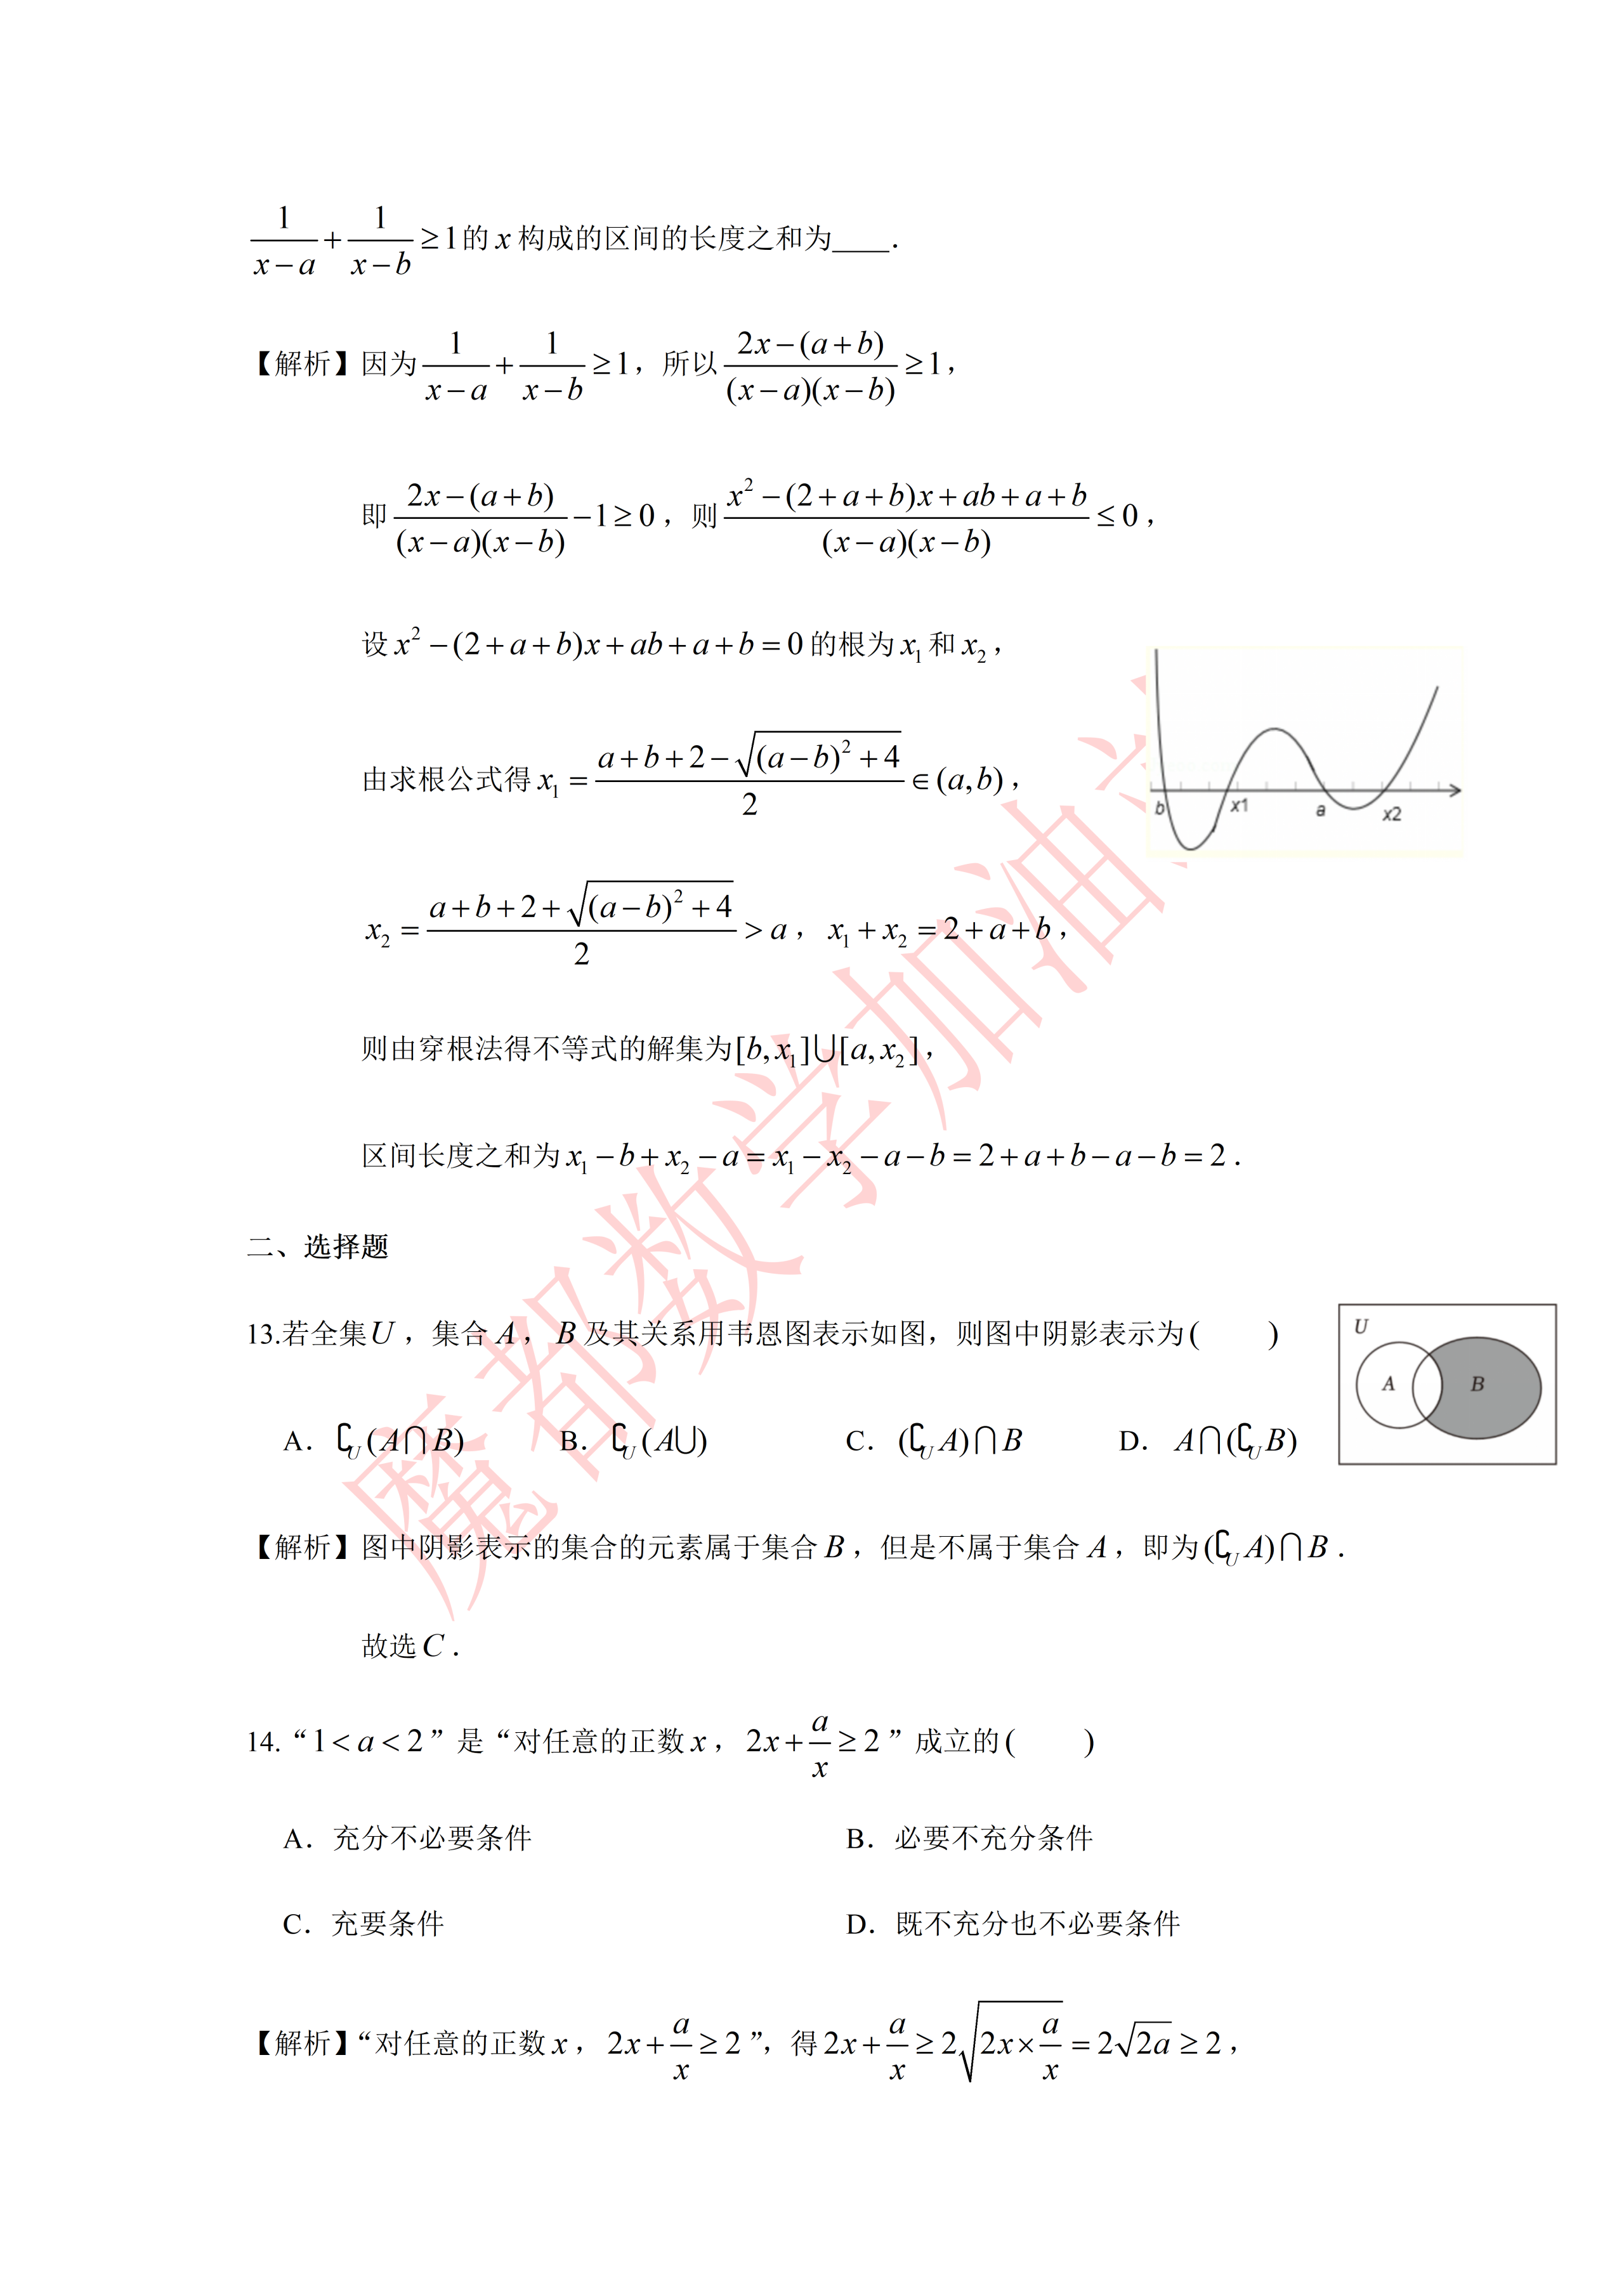
\includegraphics[width=.50\linewidth,trim=1786bp 2255bp 228bp 985bp,clip]{../原图/高一51_华师大二附中_国庆作业3/04.png}
\end{center}
\step{由求根公式得 $x_1=\dfrac{a+b+2-\sqrt{(a-b)^2+4}}{2}\in(a,b)$，}
\step{$x_2=\dfrac{a+b+2+\sqrt{(a-b)^2+4}}{2}>a$，$x_1+x_2=2+a+b$，}
\step{则由穿根法得不等式的解集为 $[b,x_1]\cup[a,x_2]$，}
% 原卷如此，照录未改（此处原卷作 $x_1-x_2$，按上一行 $x_1+x_2=2+a+b$ 当为 $x_1+x_2$）
\step{区间长度之和为 $x_1-b+x_2-a=x_1-x_2-a-b=2+a+b-a-b=2$.}
\solend

\fi

\end{enumerate}

\bigsec{二、选择题}

\begin{enumerate}
\setcounter{enumi}{12}

% 本题是“题干 + 图 + 选项”约 5.5cm 的一整块，图夹在题干与选项之间时 \keepwithprev 挡不住断点，
% 故按 高一30 第 13 题的成例在题前先量一次页高（守卫放在 \item 之前）。
\needvspace{6cm}
\item 若全集 $U$，集合 $A$、$B$ 及其关系用韦恩图表示如图，则图中阴影表示为\mbox{（\quad）}

\begin{center}
% 原卷该图印在题干与选项右侧（原图第 04 页），本稿移作居中排，直接裁取原图，不另存图片文件。
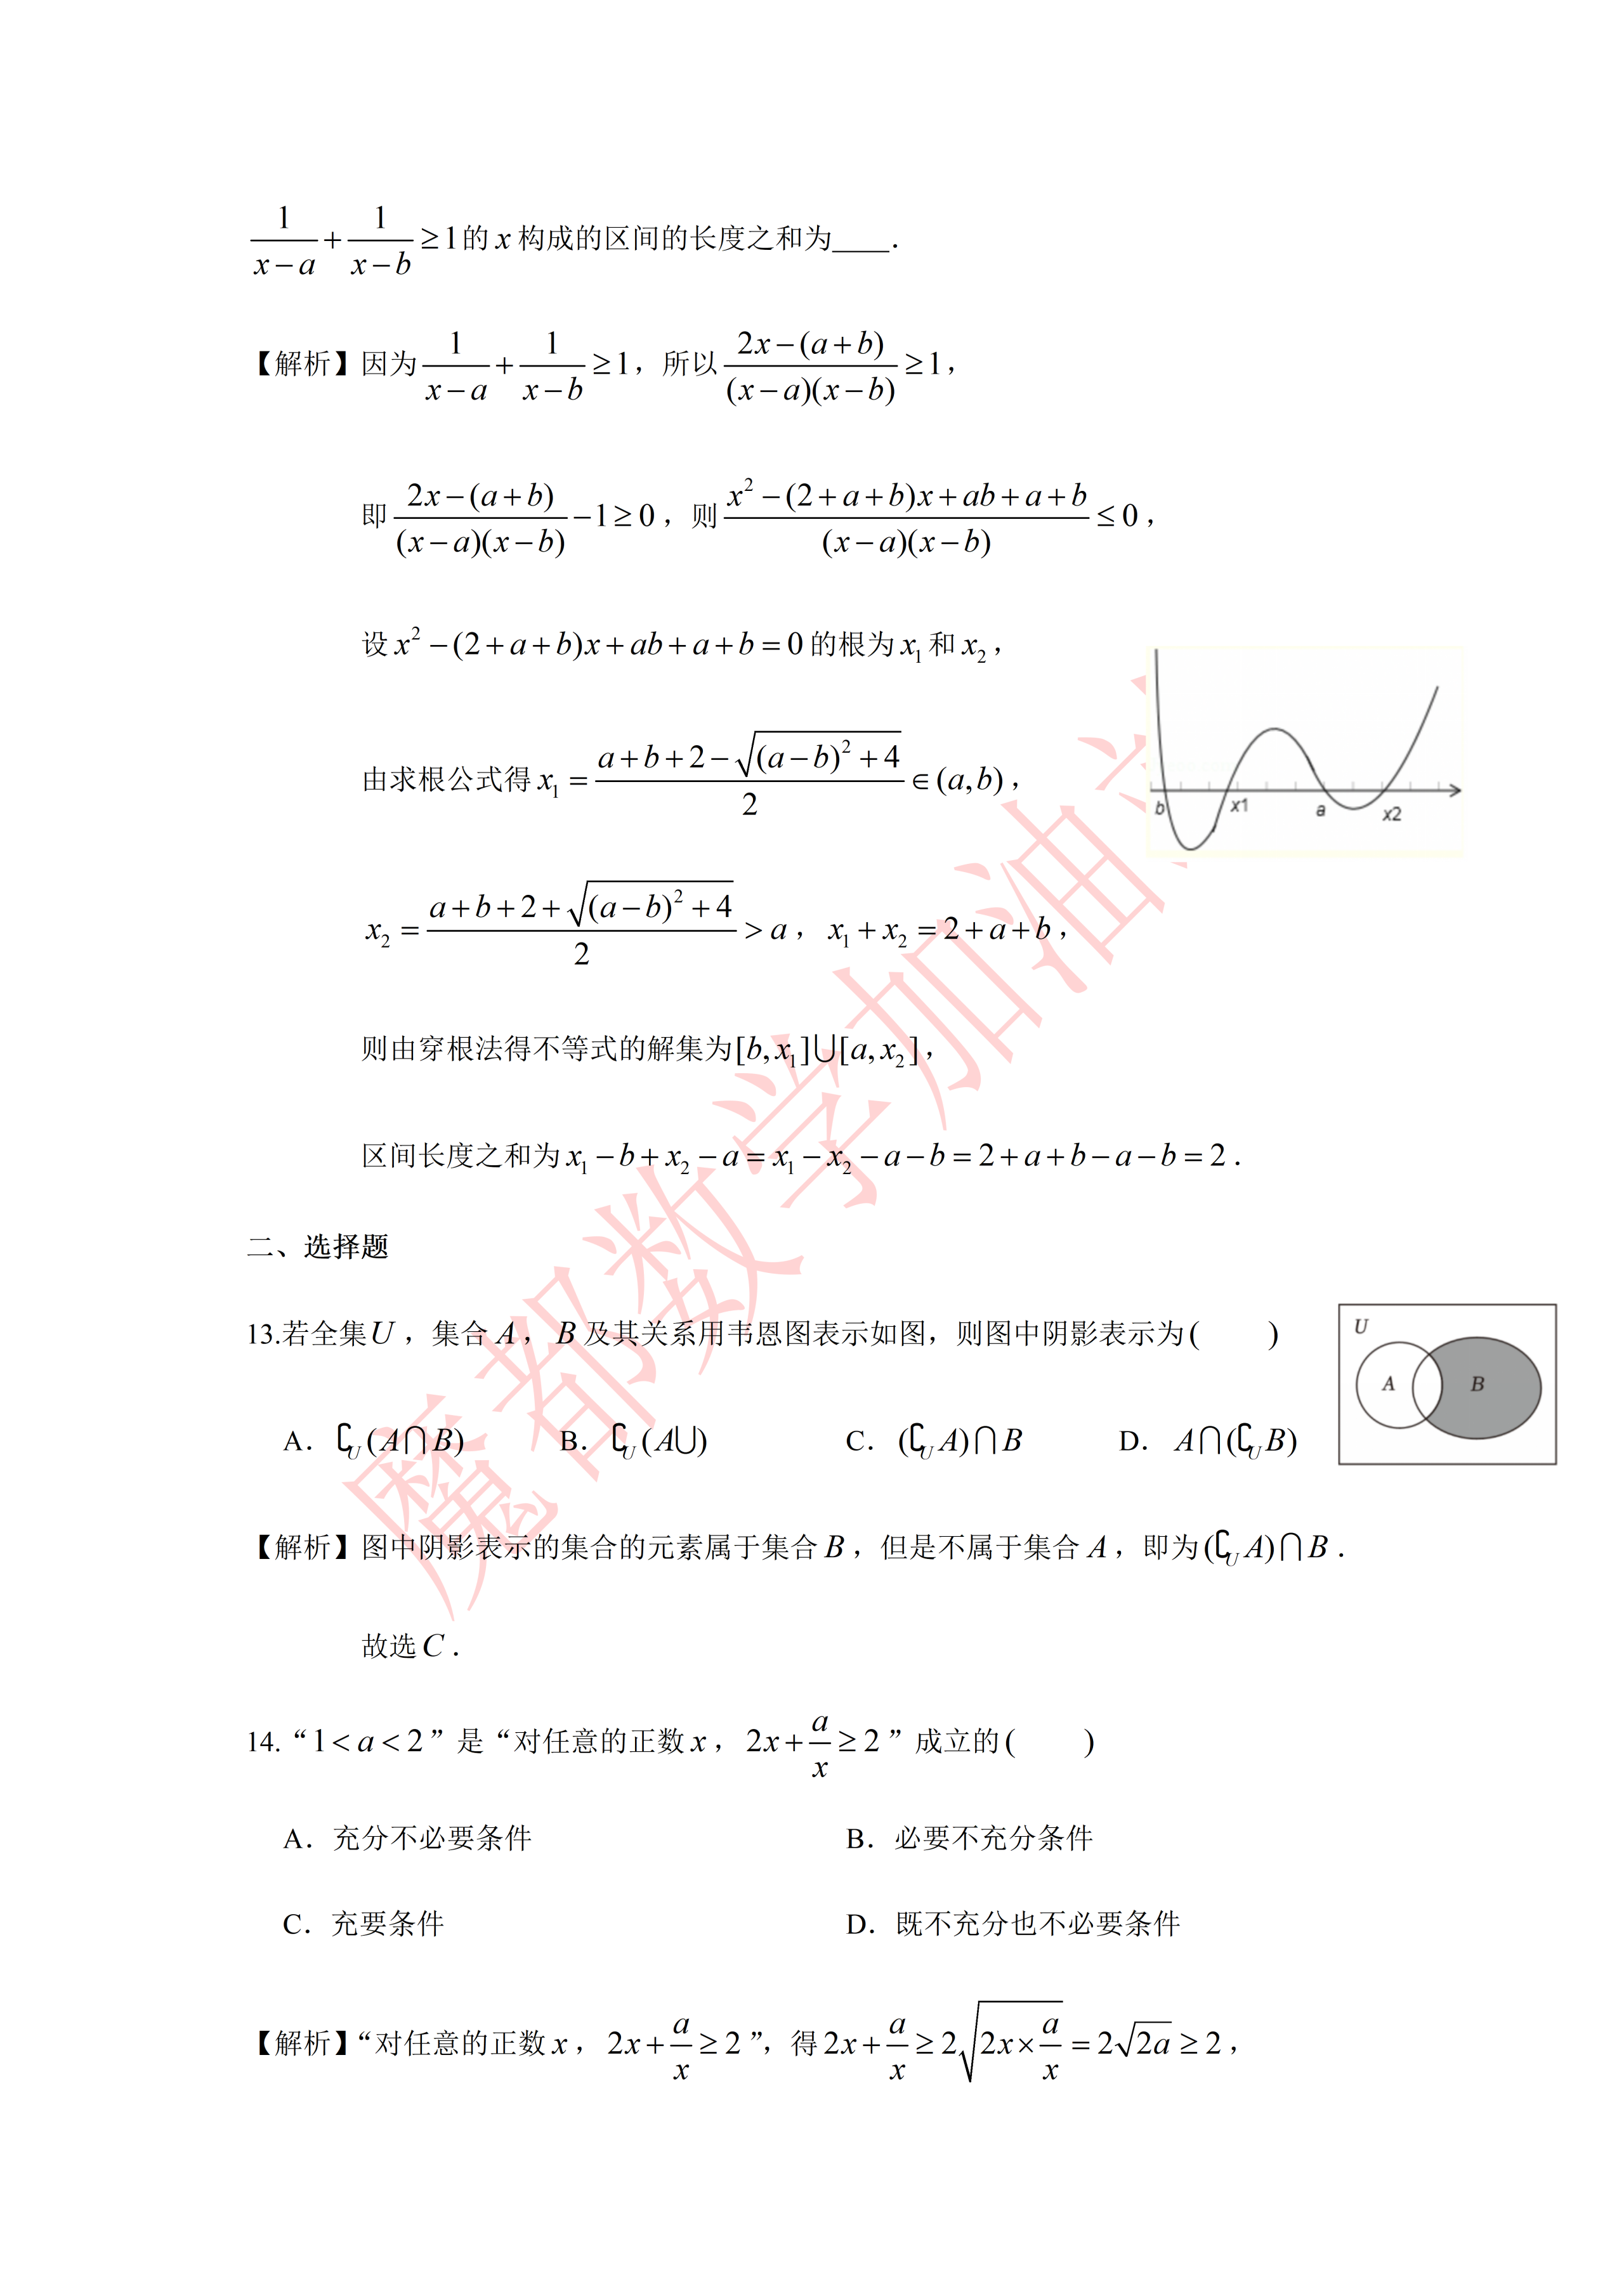
\includegraphics[width=.30\linewidth,trim=2105bp 1308bp 105bp 2050bp,clip]{../原图/高一51_华师大二附中_国庆作业3/04.png}
\end{center}

\keepwithprev
A. $\complement_U(A\cap B)$\qquad B. $\complement_U(A\cup B)$

C. $(\complement_U A)\cap B$\qquad D. $A\cap(\complement_U B)$

\ifanswer
\solbegin
\step{图中阴影表示的集合的元素属于集合 $B$，但是不属于集合 $A$，即为 $(\complement_U A)\cap B$.}
\step{故选 $C$.}
\solend

\fi

\item “$1<a<2$”是“对任意的正数 $x$，$2x+\dfrac ax\geqslant2$”成立的\mbox{（\quad）}

\keepwithprev
A. 充分不必要条件\qquad B. 必要不充分条件

C. 充要条件\qquad\qquad D. 既不充分也不必要条件

\ifanswer
\solbegin
\step{“对任意的正数 $x$，$2x+\dfrac ax\geqslant2$”，得 $2x+\dfrac ax\geqslant2\sqrt{2x\times\dfrac ax}=2\sqrt{2a}\geqslant2$，}
\step{所以 $\sqrt{2a}\geqslant1$，解得 $a\geqslant\dfrac12$，}
\step{若“$1<a<2$”得 $2x+\dfrac ax\geqslant2\sqrt{2x\times\dfrac ax}=2\sqrt{2a}>2\sqrt2>2$，}
\step{所以“$1<a<2$”$\Rightarrow$“对任意的正数 $x$，$2x+\dfrac ax\geqslant2$”，}
\step{所以“$1<a<2$”是“对任意的正数 $x$，$2x+\dfrac ax\geqslant2$”成立的充分不必要条件，}
\step{故选 $A$.}
\solend

\fi

\item 已知函数 $f(x)=2x-3$，$x\in(0,2)$，实数 $a$、$b$ 满足 $f(a)+f(b-1)=0$，则以下成立的有\mbox{（\quad）}

\keepwithprev
A. $a(b-1)$ 的最大值为 $\dfrac94$\qquad\qquad B. $b-\dfrac1a$ 的最大值为 $2$

C. $\dfrac1a+\dfrac1{4b}$ 的最小值为 $\dfrac9{16}$\qquad D. $-1<b-a<3$

\ifanswer
\solbegin
\step{因为函数 $f(x)=2x-3$，$x\in(0,2)$，实数 $a$、$b$ 满足 $f(a)+f(b-1)=0$，}
\step{所以 $2a-3+2(b-1)-3=0$，得 $a+b=4$，$a\in(0,2)$，$b\in(1,3)$，}
\step{所以 $a(b-1)=a(3-a)=-\left(a-\dfrac32\right)^2+\dfrac94$，$a\in(0,2)$，}
\step{所以 $0<a(b-1)\leqslant\dfrac94$，故选项 $A$ 正确；}
\step{$b-\dfrac1a=4-a-\dfrac1a=4-\left(a+\dfrac1a\right)\leqslant4-2=2$，}
\step{当且仅当 $a=1$，$b=3$ 时取等号，又 $b\in(1,3)$，故 $b-\dfrac1a<2$，故 $B$ 错误；}
\step{$\dfrac1a+\dfrac1{4b}=\dfrac14\left(\dfrac1a+\dfrac1{4b}\right)(a+b)=\dfrac14\left(1+\dfrac14+\dfrac ba+\dfrac a{4b}\right)=\dfrac5{16}+\dfrac14\left(\dfrac ba+\dfrac a{4b}\right)$}
\step{$\geqslant\dfrac5{16}+\dfrac14\cdot2\sqrt{\dfrac ba\cdot\dfrac a{4b}}=\dfrac9{16}$，当且仅当 $\dfrac ba=\dfrac a{4b}$，即 $a=2b=\dfrac83$ 时取等号，}
% 原卷如此，照录未改（“又 $a\in(0,2)$，”与下式之间原卷正文夹印“水印”二字）
\step{又 $a\in(0,2)$，水印 $\dfrac1a+\dfrac1{4b}<\dfrac9{16}$，故 $C$ 错误；}
\step{因为 $a\in(0,2)$，$b\in(1,3)$，所以 $-a\in(-2,0)$，所以 $b-a\in(-1,3)$，}
\step{故 $D$ 正确；}
\step{故选 $AD$.}
\solend

\fi

% 本题解析含图（“函数 f(x) 的图像如下”），图夹在解析行间，页末放不下会被拆开，
% 故在题前先量一次页高；上界取“题干 + 选项 + 图 + 首行解析”一块的高度。
\needvspace{6cm}
\item 设 $M_I$ 表示函数 $f(x)=|x^2-4x+2|$ 在闭区间 $I$ 上的最大值. 若正实数 $a$ 满足
$M_{[0,a]}\geqslant2M_{[a,2a]}$，则正实数 $a$ 的取值范围是\mbox{（\quad）}

\keepwithprev
A. $\left[2-\sqrt3,\dfrac12\right]$\qquad B. $[2-\sqrt3,1]$

C. $[2,2+\sqrt3]$\qquad\qquad D. $[2+\sqrt3,4]$

\ifanswer
\solbegin
\step{函数 $f(x)$ 的图像如下：}
\begin{center}
% 原卷该图印在解析行间（原图第 06 页），本稿直接裁取原图，不另存图片文件。
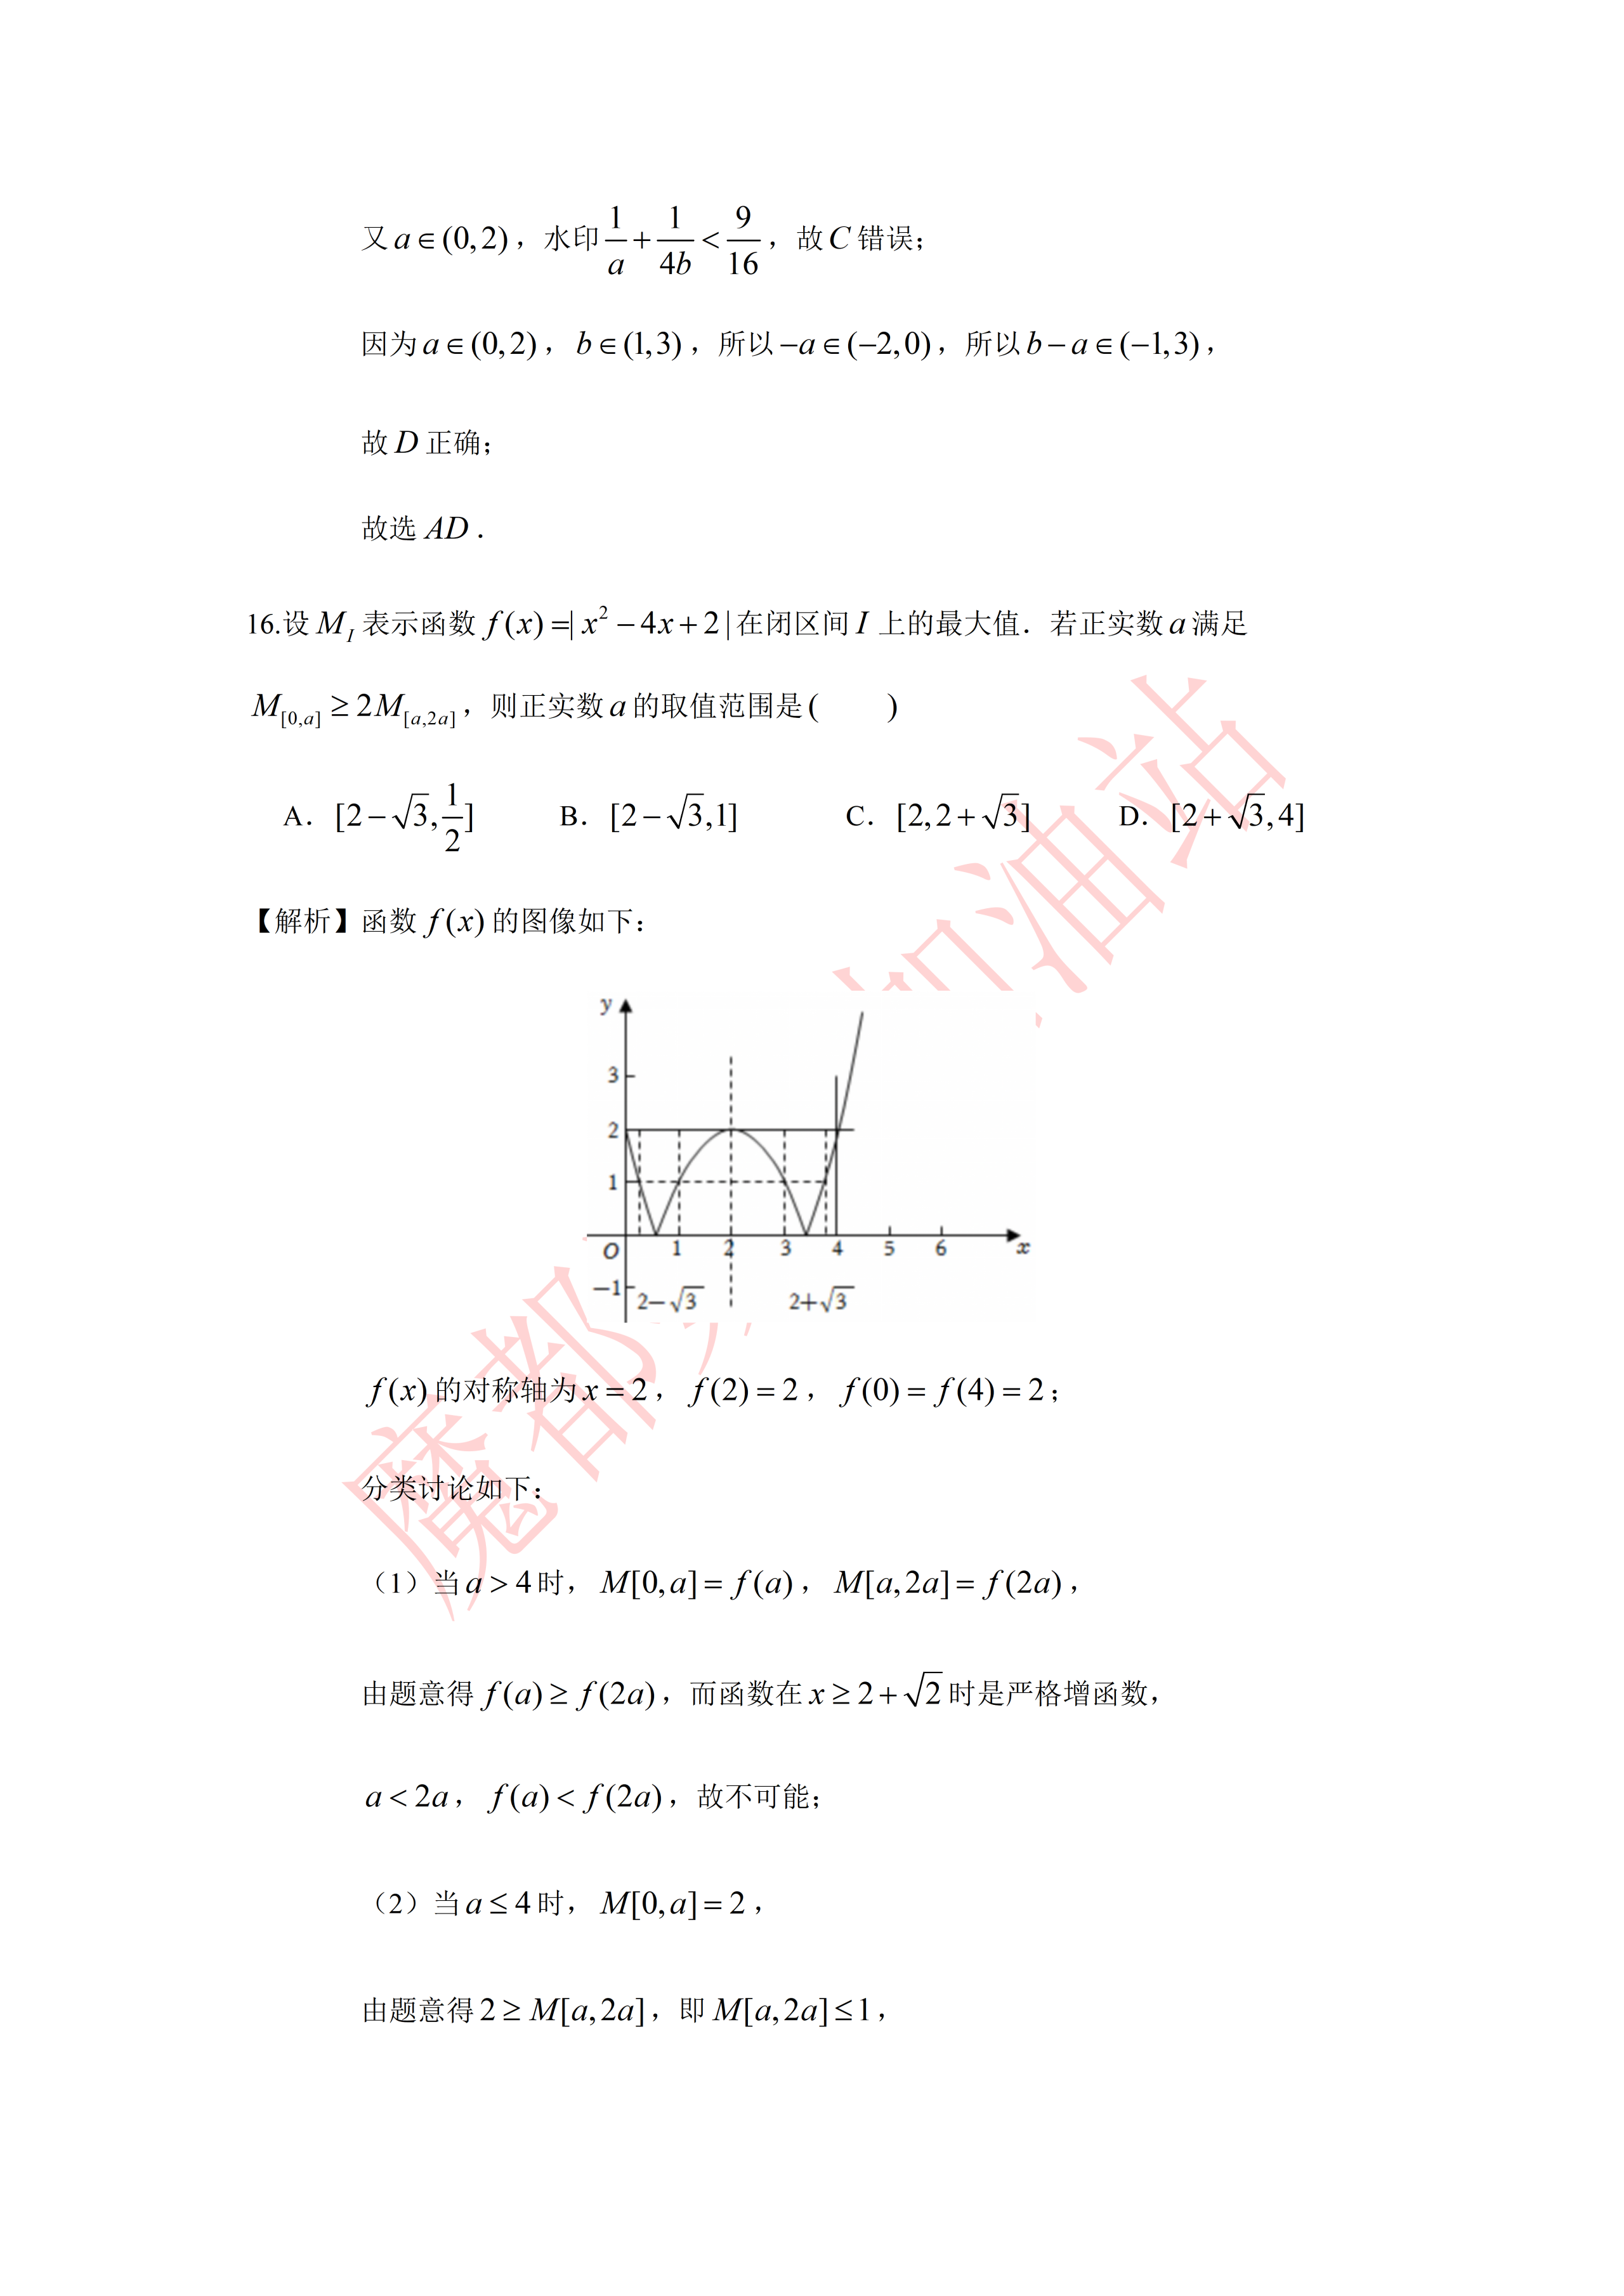
\includegraphics[width=.55\linewidth,trim=895bp 1535bp 915bp 1525bp,clip]{../原图/高一51_华师大二附中_国庆作业3/06.png}
\end{center}
\step{$f(x)$ 的对称轴为 $x=2$，$f(2)=2$，$f(0)=f(4)=2$；}
\step{分类讨论如下：}
\stepm{(1)}{当 $a>4$ 时，$M_{[0,a]}=f(a)$，$M_{[a,2a]}=f(2a)$，}
\step{由题意得 $f(a)\geqslant f(2a)$，而函数在 $x\geqslant2+\sqrt2$ 时是严格增函数，}
\step{$a<2a$，$f(a)<f(2a)$，故不可能；}
\stepm{(2)}{当 $a\leqslant4$ 时，$M_{[0,a]}=2$，}
\step{由题意得 $2\geqslant M_{[a,2a]}$，即 $M_{[a,2a]}\leqslant1$，}
\step{令 $f(x)=1$，解得 $x_1=2-\sqrt3$，$x_2=1$，$x_3=2+\sqrt3$，$x_4=3$，}
\step{则有 $a\geqslant2-\sqrt3$ 并且 $2a\leqslant1$，解得 $2-\sqrt3\leqslant a\leqslant\dfrac12$；}
\step{或者 $a\geqslant3$ 并且 $2a\leqslant2+\sqrt3$，无解；}
\step{故选 $A$.}
\solend

\fi

\end{enumerate}

\bigsec{三、解答题}

\begin{enumerate}
\setcounter{enumi}{16}

\item 已知 $M=\{x\mid2\leqslant x\leqslant5\}$，$N=\{x\mid a-1\leqslant x\leqslant2a+1\}$.
\begin{enumerate}[label=(\arabic*)]
\item 若 $M\subseteq N$，求实数 $a$ 的取值范围；
\item 若 $M\supseteq N$，求实数 $a$ 的取值范围.
\end{enumerate}

\ifanswer
\ans{（1）$[2,3]$；（2）$(-\infty,-2)$}
\fi

\ansspace[6]

\item 设集合 $A=\{x\mid|x+1|\leqslant3\}$，$B=\{x\mid0<x<3m\}$.
\begin{enumerate}[label=(\arabic*)]
\item 若 $A\cup B=A$，求实数 $m$ 的取值范围；
\item 设 $P=(\complement_R A)\cap B$，若 $\exists x\in\Z$ 且 $x\in P$，求实数 $m$ 的取值范围.
\end{enumerate}

\ifanswer
\solbegin
\stepm{(1)}{$A=\{x\mid|x+1|\leqslant3\}=\{x\mid-4\leqslant x\leqslant2\}$，且 $A\cup B=A$，所以 $B\subseteq A$.}
\step{若 $B=\varnothing$，此时 $0\geqslant3m$，解得 $m\leqslant0$；}
\step{若 $B\neq\varnothing$，此时 $0<3m$，且 $3m\leqslant2$，解得 $0<m\leqslant\dfrac23$；}
\step{则实数 $m$ 的取值范围是 $\left(-\infty,\dfrac23\right]$.}
\stepm{(2)}{因为 $\exists x\in\Z$ 且 $x\in P$，所以集合 $P$ 中至少存在一个整数.}
\step{$\complement_R A=\{x\mid x<-4\text{ 或 }x>2\}$，$B=\{x\mid0<x<3m\}$，}
\step{要使 $P=(\complement_R A)\cap B$ 中至少存在一个整数，则 $\begin{cases}3m>0\\3m>3\end{cases}$，解得 $m>1$，}
\step{则实数 $m$ 的取值范围是 $(1,+\infty)$.}
\solend

\fi

\ansspace[7]

\item 已知函数 $f(x)=x^2+(1-a)x-a(a\in\R)$.
\begin{enumerate}[label=(\arabic*)]
\item 解关于 $x$ 的不等式 $f(x)<0$；
\item 若 $\forall a\in[-1,1]$，$f(x)\geqslant0$ 恒成立，求实数 $x$ 的取值范围.
\end{enumerate}

\ifanswer
\solbegin
\stepm{(1)}{不等式 $x^2+(1-a)x-a<0$ 等价于 $(x-a)(x+1)<0$，}
\step{当 $a<-1$ 时，不等式的解集为 $(a,-1)$；}
\step{当 $a=-1$ 时，不等式的解集为 $\varnothing$；}
\step{当 $a>-1$ 时，不等式的解集为 $(-1,a)$.}
\stepm{(2)}{$x^2+(1-a)x-a=-a(x+1)+x^2+x$，}
\step{设 $g(a)=-a(x+1)+x^2+x$，$a\in[-1,1]$，}
\step{要使 $g(a)\geqslant0$ 在 $a\in[-1,1]$ 上恒成立，}
\step{只需 $\begin{cases}g(-1)\geqslant0\\g(1)\geqslant0\end{cases}$，即 $\begin{cases}x^2+2x+1\geqslant0\\x^2-1\geqslant0\end{cases}$，解得 $x\geqslant1$ 或 $x\leqslant-1$，}
\step{所以 $x$ 的取值范围为 $\{x\mid x\leqslant-1\text{ 或 }x\geqslant1\}$.}
\solend

\fi

\ansspace[7]

\item 若实数 $x$、$y$、$m$ 满足 $|x-m|>|y-m|$，则称 $x$ 比 $y$ 远离 $m$.
\begin{enumerate}[label=(\arabic*)]
\item 若 $2$ 比 $3x-4$ 远离 $1$，求 $x$ 的取值范围；
\item 设 $y=\dfrac{x+2}{x+1}$，其中 $x\in(0,\sqrt2)\cup(\sqrt2,+\infty)$，判断：$x$ 与 $y$ 哪一个更远离 $\sqrt2$？并说明理由.
\item 若 $x+y=2$，试问：$y$ 与 $x^2+y^2$ 哪一个更远离 $\dfrac12$？并说明理由.
\end{enumerate}

\ifanswer
\solbegin
\stepm{(1)}{由题意得 $|2-1|>|3x-4-1|$，所以 $|3x-5|<1$，解得 $\dfrac43<x<2$，}
\step{故 $x$ 的取值范围为 $\left(\dfrac43,2\right)$；}
\stepm{(2)}{$x$ 比 $y$ 更远离 $\sqrt2$，}
\step{理由如下：要证 $x$ 比 $y$ 更远离 $\sqrt2$，只要证 $|x-\sqrt2|>\left|\dfrac{x+2}{x+1}-\sqrt2\right|$，}
\step{即证 $|x-\sqrt2|>\left|\dfrac{(1-\sqrt2)(x-\sqrt2)}{x+1}\right|$，}
\step{因为 $x\in(0,\sqrt2)\cup(\sqrt2,+\infty)$，所以 $|x-\sqrt2|>0$，}
\step{所以只要证 $1>\dfrac{\sqrt2-1}{|x+1|}$，即证 $|x+1|>\sqrt2-1$，}
\step{因为 $x\in(0,\sqrt2)\cup(\sqrt2,+\infty)$，所以 $x+1\in(1,\sqrt2+1)\cup(\sqrt2+1,+\infty)$，}
\step{所以 $|x+1|>1>\sqrt2-1$，所以 $x$ 比 $y$ 更远离 $\sqrt2$；}
\stepm{(3)}{因为 $x^2+y^2\geqslant\dfrac{(x+y)^2}{2}=2$，当且仅当 $x=y=1$ 时等号成立，}
\step{所以 $\left|x^2+y^2-\dfrac12\right|=x^2+y^2-\dfrac12$，}
\step{从而 $\left|y-\dfrac12\right|-\left|x^2+y^2-\dfrac12\right|=\left|y-\dfrac12\right|-\left(x^2+y^2-\dfrac12\right)$，}
\step{①$y\geqslant\dfrac12$，$\left|y-\dfrac12\right|-\left|x^2+y^2-\dfrac12\right|=y-\dfrac12-\left(x^2+y^2-\dfrac12\right)=y-x^2-y^2$}
\step{$=y-(2-y)^2-y^2=-2y^2+5y-4=-2\left(y-\dfrac54\right)^2-\dfrac78<0$，}
\step{即 $\left|y-\dfrac12\right|<\left|x^2+y^2-\dfrac12\right|$；}
\step{②$y<\dfrac12$，}
\step{$\left|y-\dfrac12\right|-\left|x^2+y^2-\dfrac12\right|=\left(\dfrac12-y\right)-\left(x^2+y^2-\dfrac12\right)=-y-x^2-y^2+1$}
\step{$=-y-(2-y)^2-y^2+1=-2y^2+3y-3=-2\left(y-\dfrac34\right)^2-\dfrac{15}8<0$，}
\step{即 $\left|y-\dfrac12\right|<\left|x^2+y^2-\dfrac12\right|$；}
\step{综上，$\left|y-\dfrac12\right|<\left|x^2+y^2-\dfrac12\right|$，即 $x^2+y^2$ 比 $y$ 更远离 $\dfrac12$.}
\solend

\fi

\ansspace[9]

\item 对于非空有限整数集 $X$，$m\in\N^*$，定义 $X^m=\{x^m\mid x\in X\}$，对 $n\in\Z$，
$Y\oplus n=\{x+n\mid x\in Y\}$ 现有两个非空有限整数集 $A$、$B$，已知 $A\oplus1\subseteq B$ 且
$B^2\oplus(-4)\subseteq A$.
\begin{enumerate}[label=(\arabic*)]
\item 当 $A=\{-3,0\}$ 时求集合 $B$；
\item 证明：$A\subseteq\{-3,-2,0,1\}$；
\item 当 $A\oplus1=B$ 且 $B^2\oplus(-4)=A$ 时，任取 $a\in A$，$b\in B$ 构造函数
$f(x)=(x-a)(x-b)$ 问：当 $a$、$b$ 取何值时，$f(x)$ 的最小值最小？
\end{enumerate}

\ifanswer
\solbegin
\stepm{(1)}{因为 $A=\{-3,0\}$，$B^2\oplus(-4)\subseteq A$，}
\step{所以 $B^2\oplus(-4)$ 可能为 $\varnothing$、$\{-3\}$、$\{0\}$、$\{-3,0\}$，}
\step{当 $B^2\oplus(-4)=\varnothing$ 时 $B^2=\varnothing$，不满足非空，不合题意；}
\step{当 $B^2\oplus(-4)=\{-3\}$ 时 $B^2=\{1\}$，所以 $B=\{1,-1\}$、$\{1\}$、$\{-1\}$，}
\step{当 $B^2\oplus(-4)=\{0\}$ 时 $B^2=\{4\}$，所以 $B=\{2,-2\}$、$\{2\}$、$\{-2\}$，}
% 原卷如此，照录未改（此处作 $\{0,-3\}$，上一行同一集合作 $\{-3,0\}$）
\step{当 $B^2\oplus(-4)=\{0,-3\}$ 时 $B^2=\{4,1\}$，}
\step{所以 $B=\{1,2,-1,-2\}$、$\{2,-1,-2\}$、$\{2,1,-2\}$、$\{1,-1,-2\}$、$\{1,-1,2\}$、$\{1,2\}$、$\{-1,2\}$、$\{-1,-2\}$、$\{1,-2\}$，}
\step{又 $A\oplus1=\{-2,1\}\subseteq B$，得 $B$ 为 $\{1,-2\}$、$\{2,1,-2\}$、$\{1,-1,-2\}$、$\{1,2,-1,-2\}$.}
\stepm{(2)}{设 $x\in A$，因为 $A\oplus1\subseteq B$，所以 $x+1\in B$，}
\step{又 $B^2\oplus(-4)\subseteq A$，所以 $(x+1)^2-4\in A$，}
% 原卷如此，照录未改（此处及下文取 $x=2$ 处原卷均作 $(-4+1)^2-4=52-2a>0$）
\step{取 $x=-4$，则 $(-4+1)^2-4=52-2a>0$，$(5+1)^2-4=32\in A$，$\cdots$，}
\step{无限迭代，而 $A$ 为有限集，不合题意，舍去，即 $-4\notin A$；}
\step{取 $x=-3$，则 $(-3+1)^2-4=0\in A$，$(0+1)^2-4=-3\in A$，}
\step{得 $A$ 集合可为 $\{-3,0\}$；}
\step{取 $x=-2$，则 $(-2+1)^2-4=-3\in A$，$(-3+1)^2-4=0\in A$，}
\step{$(0+1)^2-4=-3\in A$，得 $A$ 集合可为 $\{-3,-2,0\}$；}
\step{取 $x=-1$，则 $(-1+1)^2-4=-4\in A$，又 $-4\notin A$，所以 $-1\notin A$，}
\step{取 $x=1$，则 $(1+1)^2-4=0\in A$，$(0+1)^2-4=-3\in A$，}
\step{$(-3+1)^2-4=0\in A$，得 $A$ 集合可为 $\{-3,0,1\}$，}
\step{取 $x=2$，则 $(2+1)^2-4=52-2a>0$，$(5+1)^2-4=32\in A$，$\cdots$，}
\step{无限迭代，而 $A$ 为有限集，不合题意，舍去，即 $2\notin A$，}
\step{同理当 $x<-4$ 或 $x>2$，且 $x\in\Z$ 时不符合 $A$ 为有限集，舍去；}
\step{故由上得 $A$ 集合可为 $\{-3,0\},\{-3,-2,0\},\{-3,0,1\},\{-3,-2,0,1\}$，}
\step{所以 $A\subseteq\{-3,-2,0,1\}$，}
\stepm{(3)}{当 $A\oplus1=B$ 且 $B^2\oplus(-4)=A$ 时，}
\step{设 $x\in B$，则 $x^2-4\in B^2\oplus(-4)=A$，}
% 原卷如此，照录未改（题设 $A=\{-3,0\}$，此处两个判别式取的是 $-2$ 与 $1$，均不属于 $A$）
\step{$x^2-4=-2$ 时 $x=\pm\sqrt2$，不为整数，不合题意；}
\step{$x^2-4=1$ 时 $x=\pm\sqrt5$，不为整数，不合题意；}
\step{所以 $A=\{-3,0\}$，又 $A\oplus1=B$，则 $B=\{-2,1\}$，}
\step{任取 $a\in A$，$b\in B$ 构造函数 $f(x)=(x-a)(x-b)$，}
\step{$f(x)=(x-a)(x-b)=x^2-(a+b)x+ab$}
\step{$=x^2-(a+b)x+\dfrac{(a+b)^2}{4}+ab-\dfrac{(a+b)^2}{4}$}
\step{$=\left[x-\dfrac{(a+b)}2\right]^2-\dfrac{(a-b)^2}{4}\geqslant-\dfrac{(a-b)^2}{4}$，所以 $f(x)_{min}=-\dfrac{(a-b)^2}{4}$，}
\step{又 $a\in A=\{-3,0\}$，$b\in B=\{-2,1\}$，所以 $a-b$ 的取值有 $-1,-4,2$，}
\step{所以 $f(x)_{min}=-\dfrac{(a-b)^2}{4}\geqslant-\dfrac{(-3-1)^2}{4}=-4$，}
\step{即当 $a=-3$，$b=1$ 时 $f(x)_{min}$ 的最小值为 $-4$.}
\solend

\fi

\ansspace*[12]

\end{enumerate}

\end{document}
"
%
% 原始材料：微信公众号“魔都数学加油站”文章，作者破晓，连载“27学年高一51”；
% 原文标题“27学年高一51——2026-2027年上海市华师大二附中高一上国庆作业3”；
% 原文链接：https://mp.weixin.qq.com/s/95SLMEmPUT30s4U7wjr5Og。
% 该页面用 JS 渲染，未见明确发布日期；页面内时间戳约为 2026-10-05 21:37，本稿以该时刻记可得日期。
% 正文为 12 张 PNG 页：第 01、02、03、05、07、08、11 页 4762×6735，
% 第 04、06、09、10、12 页 2560×3620。按页序逐页读取，12 页全为试卷正文页
% （卷首标题在第 1 页页顶，卷末解答题止于第 12 页），无封面页、目录页或单独的页脚页。
% 卷面标题照原卷印作“2026-2027 年华师大二附中高一上国庆作业 3”（公众号标题中的“上海市”
% 卷面标题行没有，本稿照卷面），年份区间按全稿惯例排 en dash。
%
% 篇幅与题号：原卷自第 3 题起编号（第 1、2 题不在本卷内）。填空题 3—12（10 题）、
% 选择题 13—16（4 题）、解答题 17—21（5 题），共 19 题。本稿沿用原节与原题号，
% 只改排为全稿统一的大节样式（原卷小节标题为“一、填空题”“二、选择题”“三、解答题”）。
% 正文为讲评版：填空题 3—12 与选择题 13—16 只印【解析】（选择题的结论“故选 X”印在解析内），
% 按全稿口径这类题不另提 \ans{}；解答题第 17 题只印【答案】，故只给 \ans{}；
% 第 18—21 题只印【解析】。
%
% 副标题：原卷未印副标题。本稿按“知识模块”口径标作“集合与常用逻辑用语、不等式”：
% 19 题中集合与常用逻辑用语 8 题（3、4、6、10、13、17、18、21），
% 不等式（含函数最值、绝对值不等式）11 题（5、7、8、9、11、12、14、15、16、19、20），
% 两类均远超三分之一，故并标。口径同 高一46_交附闵行_国庆作业3、高一48_华师大二附中_周末作业2。
%
% 与原卷的排版差异：
%   ① 原卷每题下直接印【答案】或【解析】，本稿按全稿惯例将答案与解析置于答案版；
%   ② 原卷未印副标题，本稿按“知识模块”口径补出；
%   ③ 原卷填空横线按全稿惯例排为 \blankline[4.4em]；
%   ④ 原卷 $R$、$N$、$Z$ 均排斜体，本稿按全稿惯例改用花体 $\R$、$\N$、$\Z$（同 高一48）；
%   ⑤ 原卷第 12 题解析配图、第 13 题题干韦恩图都印在正文右侧的浮动位置，第 16 题解析配图
%      印在解析行间；本稿三图一律居中排，均自原图对应页裁切（trim），不另存图片文件；
%   ⑥ 原卷解答题未留作答空白，本稿按全稿惯例加 \ansspace；
%   ⑦ 原卷第 15 题解析第 7、8 两个印刷行是一串连等式的折行，本稿按“一条 \step ＝ 一个印刷行”
%      的口径分成两条 \step。
%
% 原卷笔误/存疑（均照录未改，正文对应处另有 % 注）：
%   ① 第 12 题解析末行作“区间长度之和为 $x_1-b+x_2-a=x_1-x_2-a-b=2+a+b-a-b=2$”，
%      按上一行 $x_1+x_2=2+a+b$，此处应为 $x_1+x_2$；原卷作 $x_1-x_2$。
%   ② 第 15 题解析“又 $a\in(0,2)$，”与 $\dfrac1a+\dfrac1{4b}<\dfrac9{16}$ 之间，
%      原卷正文夹印“水印”二字（系制版遗留字样，非试卷内容）。
%   ③ 第 21 题第 (2) 问解析两处（取 $x=-4$、取 $x=2$）作“$=52-2a>0$”，
%      与题设 $(x+1)^2-4$ 的取值（按 $x=-4$ 应为 $5$）不符，当系原卷算式遗留。
%   ④ 第 21 题第 (1) 问解析先写 $B^2\oplus(-4)$ 可能为 $\{-3,0\}$，后文又作 $\{0,-3\}$，
%      同一集合两种写法。
%   ⑤ 第 21 题第 (3) 问解析：题设 $B^2\oplus(-4)=A$ 且 $A=\{-3,0\}$ 时，由 $x^2-4\in A$
%      应得 $x^2-4=-3$ 或 $0$；原卷讨论的却是 $x^2-4=-2$ 与 $x^2-4=1$（两值均不属于 $A$），
%      与题设不合。
%
% 插图：3 张，均自原图裁切（无 \begin{tikzpicture} 重排）：
%   · 第 13 题题干韦恩图（原图第 04 页，图在题干与选项右侧）
%   · 第 12 题解析配图（原图第 04 页，图在解析右侧）
%   · 第 16 题解析配图（原图第 06 页，图在解析中间）
%
\documentclass[a4paper,11pt]{article}
\usepackage{common}

\begin{document}

\examtitlest[3]{2026--2027 年华师大二附中高一上国庆作业 3}{集合与常用逻辑用语、不等式}

\bigsec{一、填空题}

\begin{enumerate}
\setcounter{enumi}{2}

\item 若 $\{x\mid x<1\text{ 或 }x>4\}\cup\{x\mid m<x<2m+3\}=R$，则实数 $m$ 的取值范围为\blankline[4.4em].

\ifanswer
\solbegin
\step{因为 $\{x\mid x<1\text{ 或 }x>4\}\cup\{x\mid m<x<2m+3\}=R$，}
\step{所以 $\begin{cases}m<1\\2m+3>4\end{cases}$，解得 $\dfrac12<m<1$，所以 $m$ 的取值范围为 $\left(\dfrac12,1\right)$.}
\solend

\fi

\item 若“$x\leqslant5$”是“$x<a$”的必要不充分条件，则 $a$ 的取值范围是\blankline[4.4em].

\ifanswer
\solbegin
\step{若“$x\leqslant5$”是“$x<a$”的必要不充分条件，则 $\{x\mid x<a\}\subset\{x\mid x\leqslant5\}$，}
\step{所以 $a\leqslant5$.}
\solend

\fi

\item 实数 $x$、$y$ 满足 $x^2+2xy+4y^2=1$，则 $x+2y$ 的取值范围是\blankline[4.4em].

\ifanswer
\solbegin
\step{因为 $x^2+2xy+4y^2=(x+2y)^2-2xy=1$，}
\step{所以 $(x+2y)^2-1=x\cdot(2y)\leqslant\left(\dfrac{x+2y}{2}\right)^2$，当且仅当 $x=2y$ 时取等号，}
\step{解得 $-\dfrac{2\sqrt3}{3}\leqslant x+2y\leqslant\dfrac{2\sqrt3}{3}$，故 $x+2y$ 的取值范围是 $\left[-\dfrac{2\sqrt3}{3},\dfrac{2\sqrt3}{3}\right]$.}
\solend

\fi

\item 若命题 $p$：“$\exists x\in\R$，$5x^2-3x+m=0$”为假命题，则实数 $m$ 的取值范围为\blankline[4.4em].

\ifanswer
\solbegin
\step{若命题 $p$：$\exists x\in\R$，$5x^2-3x+m=0$ 为假命题，}
\step{则 $5x^2-3x+m=0$ 没有实数根，故 $\Delta=9-20m<0$，解得 $m>\dfrac9{20}$.}
\solend

\fi

\item 若当 $3\leqslant m\leqslant5$ 时，$mx^2-mx+m-9<0$ 有解，则实数 $x$ 的取值范围是\blankline[4.4em].

\ifanswer
\solbegin
\step{当 $3\leqslant m\leqslant5$ 时，$mx^2-mx+m-9<0$ 有解，}
\step{即 $(x^2-x+1)m-9<0$ 在 $m\in[3,5]$ 上有解，}
\step{因为 $x^2-x+1>0$，所以一次函数 $g(m)=(x^2-x+1)m-9$ 严格增，}
\step{所以只需 $g(3)=3x^2-3x-6<0$ 即可，}
\step{即 $x^2-x-2<0$，$(x-2)(x+1)<0$，解得 $-1<x<2$，}
\step{所以实数 $x$ 的取值范围是 $(-1,2)$.}
\solend

\fi

\item 已知不等式 $\dfrac{x}{x^2+4}\leqslant a$ 对任意的 $x\in[1,3]$ 恒成立，则实数 $a$ 的范围为\blankline[4.4em].

\ifanswer
\solbegin
\step{因为 $x\in[1,3]$，所以 $\dfrac{x}{x^2+4}=\dfrac{1}{x+\dfrac4x}\leqslant\dfrac{1}{2\sqrt{x\times\dfrac4x}}=\dfrac14$，}
\step{当且仅当 $x=\dfrac4x$ 时，即 $x=2$ 时取等号，即 $\dfrac{x}{x^2+4}$ 在 $x\in[1,3]$ 的最大值为 $\dfrac14$，}
\step{又由不等式 $\dfrac{x}{x^2+4}\leqslant a$ 对任意的 $x\in[1,3]$ 恒成立，所以 $a\geqslant\dfrac14$，}
\step{即实数 $a$ 的范围为 $\left[\dfrac14,+\infty\right)$.}
\solend

\fi

\item 甲、乙两人解关于 $x$ 的不等式 $x^2+bx+c<0$，甲写错了 $b$，正确计算后得到的解为 $\{x\mid1<x<2\}$；
乙写错了 $c$，正确计算后得到的解为 $\{x\mid-4<x<1\}$. 那么不等式 $\dfrac{bx+c}{x-2}<0$ 的解为\blankline[4.4em].

\ifanswer
\solbegin
\step{由 $x^2+bx+c<0$ 的解为 $\{x\mid1<x<2\}$，}
\step{则 $1$ 和 $2$ 是方程 $x^2+bx+c=0$ 的两个根，}
\step{甲写错了 $b$，但 $c$ 是正确的，所以 $c=1\times2=2$；}
\step{由 $x^2+bx+c<0$ 的解为 $\{x\mid-4<x<1\}$，}
\step{则 $-4$ 和 $1$ 是方程 $x^2+bx+c=0$ 的两个根，}
\step{乙写错了 $c$，但 $b$ 是正确的，所以 $-b=-4+1=-3$，即 $b=3$.}
\step{由 $\dfrac{bx+c}{x-2}<0$，得 $\dfrac{3x+2}{x-2}<0$，即 $(3x+2)(x-2)<0$，解得 $-\dfrac23<x<2$.}
\step{不等式 $\dfrac{bx+c}{x-2}<0$ 的解为 $\left\{x\mid-\dfrac23<x<2\right\}$.}
\solend

\fi

\item 已知 $\dfrac{1}{x-2}\geqslant1$ 是 $|x-a|<2$ 的充分非必要条件，则实数 $a$ 的取值范围是\blankline[4.4em].

\ifanswer
\solbegin
\step{由 $\dfrac{1}{x-2}\geqslant1$ 得 $\dfrac{3-x}{x-2}\geqslant0$，解得 $2<x\leqslant3$，由 $|x-a|<2$ 得 $a-2<x<a+2$，}
\step{因为 $\dfrac{1}{x-2}\geqslant1$ 是 $|x-a|<2$ 的充分非必要条件，}
\step{所以 $\{x\mid2<x\leqslant3\}\subset\{x\mid a-2<x<a+2\}$，所以 $\begin{cases}a-2\leqslant2\\a+2>3\end{cases}$，解得 $1<a\leqslant4$，}
\step{即实数 $a$ 的取值范围是 $(1,4]$.}
\solend

\fi

\item 设 $a>0$，$b>0$，若不等式 $a(a+1)^2+b(b+1)^2\geqslant\lambda ab$ 恒成立，则实数 $\lambda$ 的最大值为\blankline[4.4em].

\ifanswer
\solbegin
\step{$a(a+1)^2+b(b+1)^2\geqslant\lambda ab\Leftrightarrow\lambda\leqslant\dfrac{a(a+1)^2+b(b+1)^2}{ab}=\dfrac{(a+1)^2}{b}+\dfrac{(b+1)^2}{a}$，}
\step{从而原问题转化为求 $\dfrac{(a+1)^2}{b}+\dfrac{(b+1)^2}{a}$ 的最小值.}
\step{因为 $\dfrac{(a+1)^2}{b}+\dfrac{(b+1)^2}{a}=\dfrac{b^2+2b+1}{a}+\dfrac{a^2+2a+1}{b}$}
\step{$=\left(\dfrac{b^2}{a}+\dfrac{a^2}{b}\right)+2\left(\dfrac ba+\dfrac ab\right)+\left(\dfrac1a+\dfrac1b\right)\geqslant2\sqrt{\dfrac{b^2}{a}\cdot\dfrac{a^2}{b}}+2\times2\sqrt{\dfrac ba\cdot\dfrac ab}+2\sqrt{\dfrac1a\cdot\dfrac1b}$}
\step{$=2\sqrt{ab}+4+\dfrac{2}{\sqrt{ab}}\geqslant2\sqrt{2\sqrt{ab}\cdot\dfrac{2}{\sqrt{ab}}}+4=8$，以上均当且仅当 $a=b$ 时取等号，}
\step{所以 $\lambda\leqslant8$，即实数 $\lambda$ 的最大值为 $8$.}
\solend

\fi

\item 定义区间 $(a,d)$、$[a,d)$、$(a,d]$、$[a,d]$ 的长度为 $d-a$（$d>a$），已知 $a>b$，则满足
$\dfrac{1}{x-a}+\dfrac{1}{x-b}\geqslant1$ 的 $x$ 构成的区间的长度之和为\blankline[4.4em].

\ifanswer
\solbegin
\step{因为 $\dfrac{1}{x-a}+\dfrac{1}{x-b}\geqslant1$，所以 $\dfrac{2x-(a+b)}{(x-a)(x-b)}\geqslant1$，}
\step{即 $\dfrac{2x-(a+b)}{(x-a)(x-b)}-1\geqslant0$，则 $\dfrac{x^2-(2+a+b)x+ab+a+b}{(x-a)(x-b)}\leqslant0$，}
\step{设 $x^2-(2+a+b)x+ab+a+b=0$ 的根为 $x_1$ 和 $x_2$，}
\begin{center}
% 原卷该图印在解析右侧（原图第 04 页），本稿移作居中排，直接裁取原图，不另存图片文件。
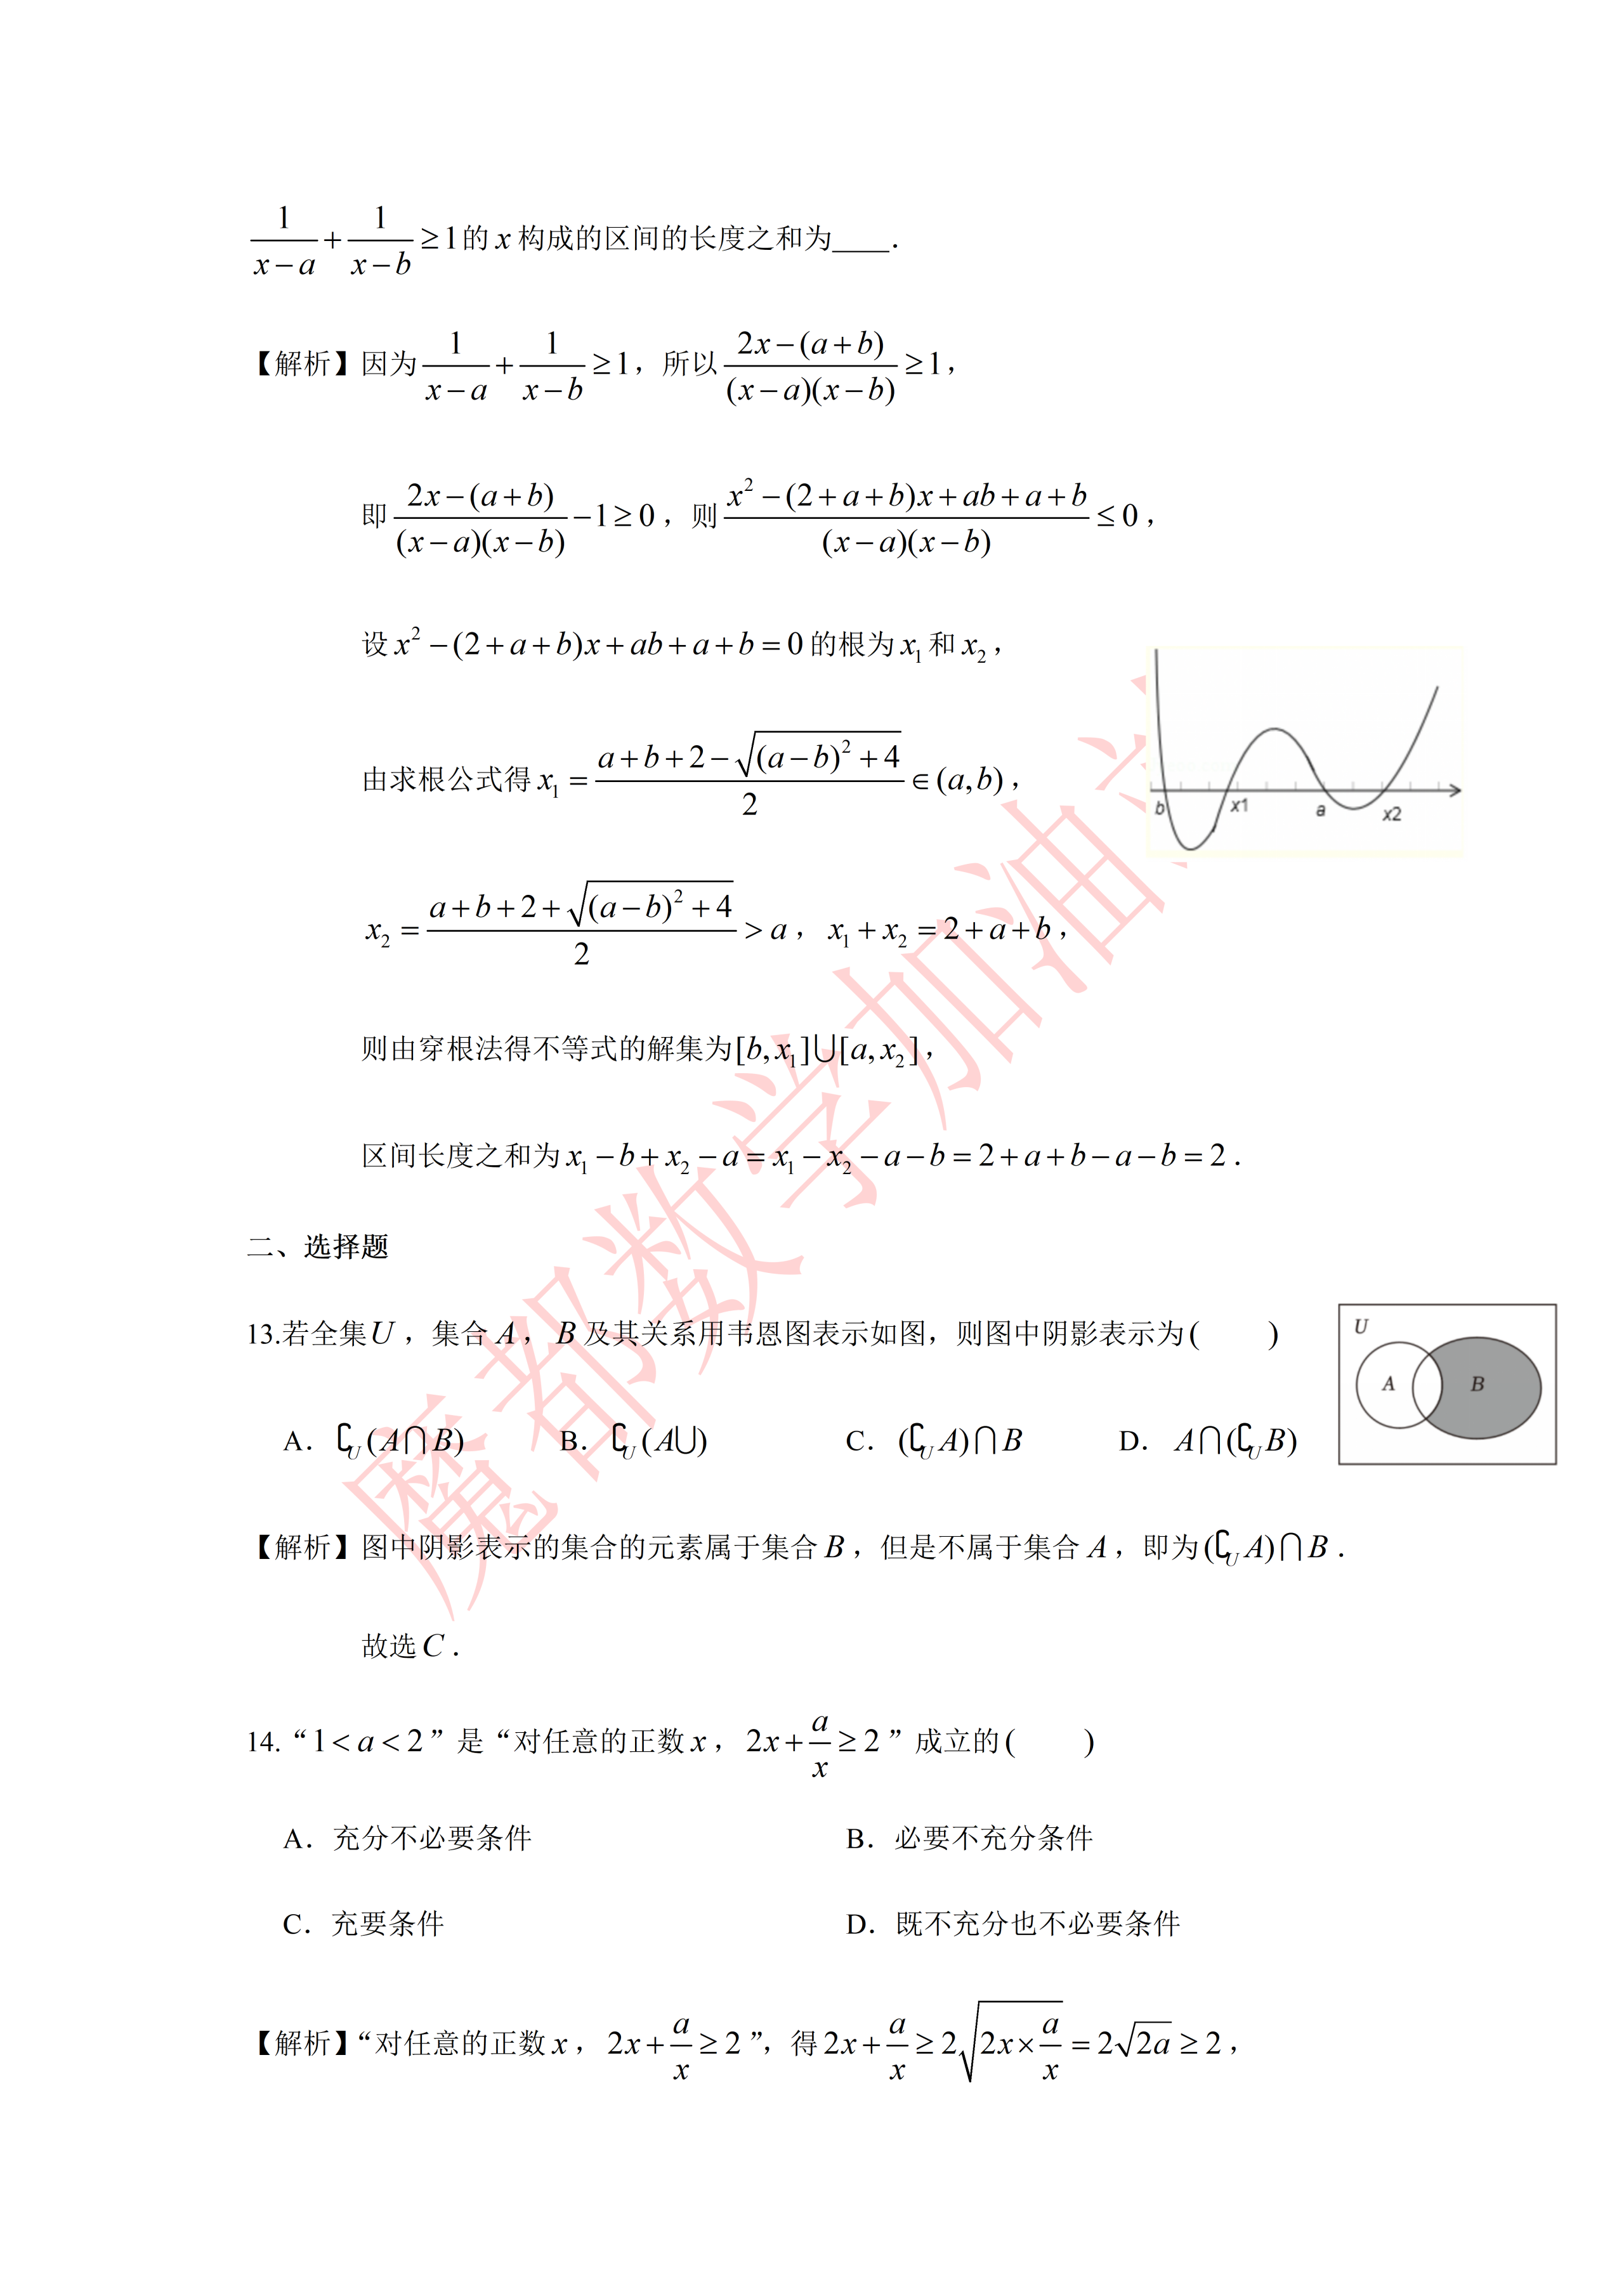
\includegraphics[width=.50\linewidth,trim=1786bp 2255bp 228bp 985bp,clip]{../原图/高一51_华师大二附中_国庆作业3/04.png}
\end{center}
\step{由求根公式得 $x_1=\dfrac{a+b+2-\sqrt{(a-b)^2+4}}{2}\in(a,b)$，}
\step{$x_2=\dfrac{a+b+2+\sqrt{(a-b)^2+4}}{2}>a$，$x_1+x_2=2+a+b$，}
\step{则由穿根法得不等式的解集为 $[b,x_1]\cup[a,x_2]$，}
% 原卷如此，照录未改（此处原卷作 $x_1-x_2$，按上一行 $x_1+x_2=2+a+b$ 当为 $x_1+x_2$）
\step{区间长度之和为 $x_1-b+x_2-a=x_1-x_2-a-b=2+a+b-a-b=2$.}
\solend

\fi

\end{enumerate}

\bigsec{二、选择题}

\begin{enumerate}
\setcounter{enumi}{12}

% 本题是“题干 + 图 + 选项”约 5.5cm 的一整块，图夹在题干与选项之间时 \keepwithprev 挡不住断点，
% 故按 高一30 第 13 题的成例在题前先量一次页高（守卫放在 \item 之前）。
\needvspace{6cm}
\item 若全集 $U$，集合 $A$、$B$ 及其关系用韦恩图表示如图，则图中阴影表示为\mbox{（\quad）}

\begin{center}
% 原卷该图印在题干与选项右侧（原图第 04 页），本稿移作居中排，直接裁取原图，不另存图片文件。
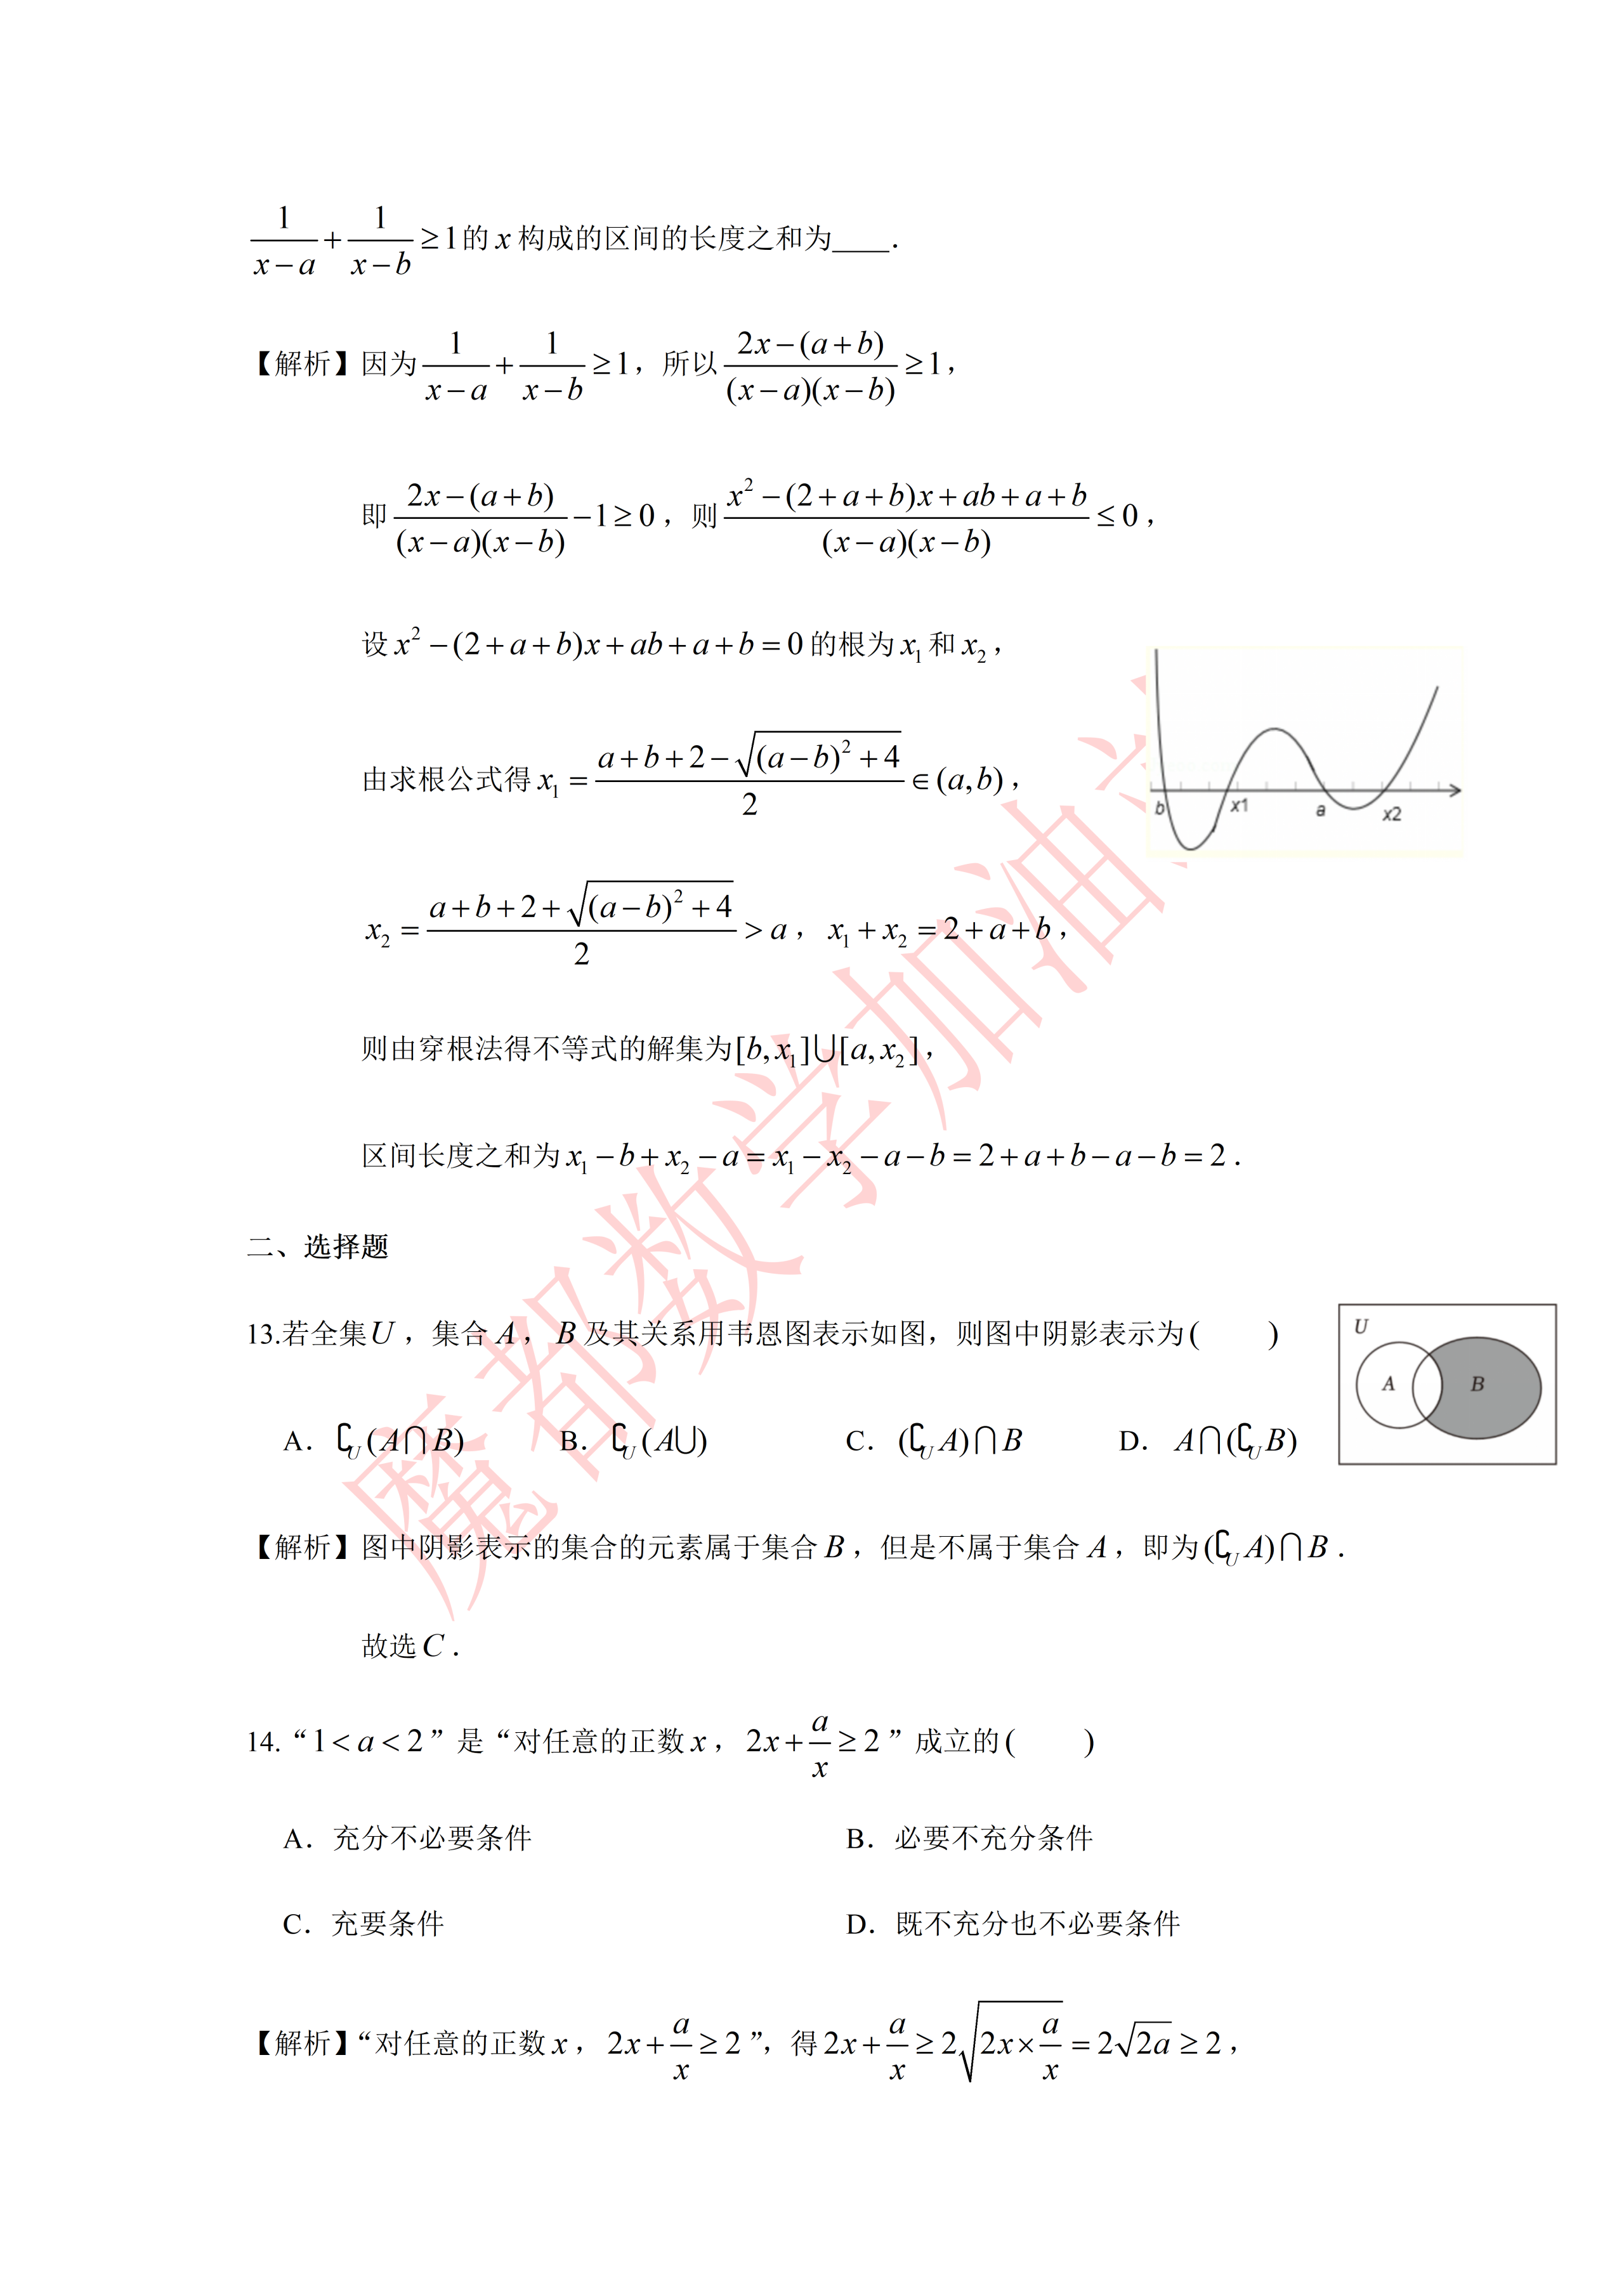
\includegraphics[width=.30\linewidth,trim=2105bp 1308bp 105bp 2050bp,clip]{../原图/高一51_华师大二附中_国庆作业3/04.png}
\end{center}

\keepwithprev
A. $\complement_U(A\cap B)$\qquad B. $\complement_U(A\cup B)$

C. $(\complement_U A)\cap B$\qquad D. $A\cap(\complement_U B)$

\ifanswer
\solbegin
\step{图中阴影表示的集合的元素属于集合 $B$，但是不属于集合 $A$，即为 $(\complement_U A)\cap B$.}
\step{故选 $C$.}
\solend

\fi

\item “$1<a<2$”是“对任意的正数 $x$，$2x+\dfrac ax\geqslant2$”成立的\mbox{（\quad）}

\keepwithprev
A. 充分不必要条件\qquad B. 必要不充分条件

C. 充要条件\qquad\qquad D. 既不充分也不必要条件

\ifanswer
\solbegin
\step{“对任意的正数 $x$，$2x+\dfrac ax\geqslant2$”，得 $2x+\dfrac ax\geqslant2\sqrt{2x\times\dfrac ax}=2\sqrt{2a}\geqslant2$，}
\step{所以 $\sqrt{2a}\geqslant1$，解得 $a\geqslant\dfrac12$，}
\step{若“$1<a<2$”得 $2x+\dfrac ax\geqslant2\sqrt{2x\times\dfrac ax}=2\sqrt{2a}>2\sqrt2>2$，}
\step{所以“$1<a<2$”$\Rightarrow$“对任意的正数 $x$，$2x+\dfrac ax\geqslant2$”，}
\step{所以“$1<a<2$”是“对任意的正数 $x$，$2x+\dfrac ax\geqslant2$”成立的充分不必要条件，}
\step{故选 $A$.}
\solend

\fi

\item 已知函数 $f(x)=2x-3$，$x\in(0,2)$，实数 $a$、$b$ 满足 $f(a)+f(b-1)=0$，则以下成立的有\mbox{（\quad）}

\keepwithprev
A. $a(b-1)$ 的最大值为 $\dfrac94$\qquad\qquad B. $b-\dfrac1a$ 的最大值为 $2$

C. $\dfrac1a+\dfrac1{4b}$ 的最小值为 $\dfrac9{16}$\qquad D. $-1<b-a<3$

\ifanswer
\solbegin
\step{因为函数 $f(x)=2x-3$，$x\in(0,2)$，实数 $a$、$b$ 满足 $f(a)+f(b-1)=0$，}
\step{所以 $2a-3+2(b-1)-3=0$，得 $a+b=4$，$a\in(0,2)$，$b\in(1,3)$，}
\step{所以 $a(b-1)=a(3-a)=-\left(a-\dfrac32\right)^2+\dfrac94$，$a\in(0,2)$，}
\step{所以 $0<a(b-1)\leqslant\dfrac94$，故选项 $A$ 正确；}
\step{$b-\dfrac1a=4-a-\dfrac1a=4-\left(a+\dfrac1a\right)\leqslant4-2=2$，}
\step{当且仅当 $a=1$，$b=3$ 时取等号，又 $b\in(1,3)$，故 $b-\dfrac1a<2$，故 $B$ 错误；}
\step{$\dfrac1a+\dfrac1{4b}=\dfrac14\left(\dfrac1a+\dfrac1{4b}\right)(a+b)=\dfrac14\left(1+\dfrac14+\dfrac ba+\dfrac a{4b}\right)=\dfrac5{16}+\dfrac14\left(\dfrac ba+\dfrac a{4b}\right)$}
\step{$\geqslant\dfrac5{16}+\dfrac14\cdot2\sqrt{\dfrac ba\cdot\dfrac a{4b}}=\dfrac9{16}$，当且仅当 $\dfrac ba=\dfrac a{4b}$，即 $a=2b=\dfrac83$ 时取等号，}
% 原卷如此，照录未改（“又 $a\in(0,2)$，”与下式之间原卷正文夹印“水印”二字）
\step{又 $a\in(0,2)$，水印 $\dfrac1a+\dfrac1{4b}<\dfrac9{16}$，故 $C$ 错误；}
\step{因为 $a\in(0,2)$，$b\in(1,3)$，所以 $-a\in(-2,0)$，所以 $b-a\in(-1,3)$，}
\step{故 $D$ 正确；}
\step{故选 $AD$.}
\solend

\fi

% 本题解析含图（“函数 f(x) 的图像如下”），图夹在解析行间，页末放不下会被拆开，
% 故在题前先量一次页高；上界取“题干 + 选项 + 图 + 首行解析”一块的高度。
\needvspace{6cm}
\item 设 $M_I$ 表示函数 $f(x)=|x^2-4x+2|$ 在闭区间 $I$ 上的最大值. 若正实数 $a$ 满足
$M_{[0,a]}\geqslant2M_{[a,2a]}$，则正实数 $a$ 的取值范围是\mbox{（\quad）}

\keepwithprev
A. $\left[2-\sqrt3,\dfrac12\right]$\qquad B. $[2-\sqrt3,1]$

C. $[2,2+\sqrt3]$\qquad\qquad D. $[2+\sqrt3,4]$

\ifanswer
\solbegin
\step{函数 $f(x)$ 的图像如下：}
\begin{center}
% 原卷该图印在解析行间（原图第 06 页），本稿直接裁取原图，不另存图片文件。
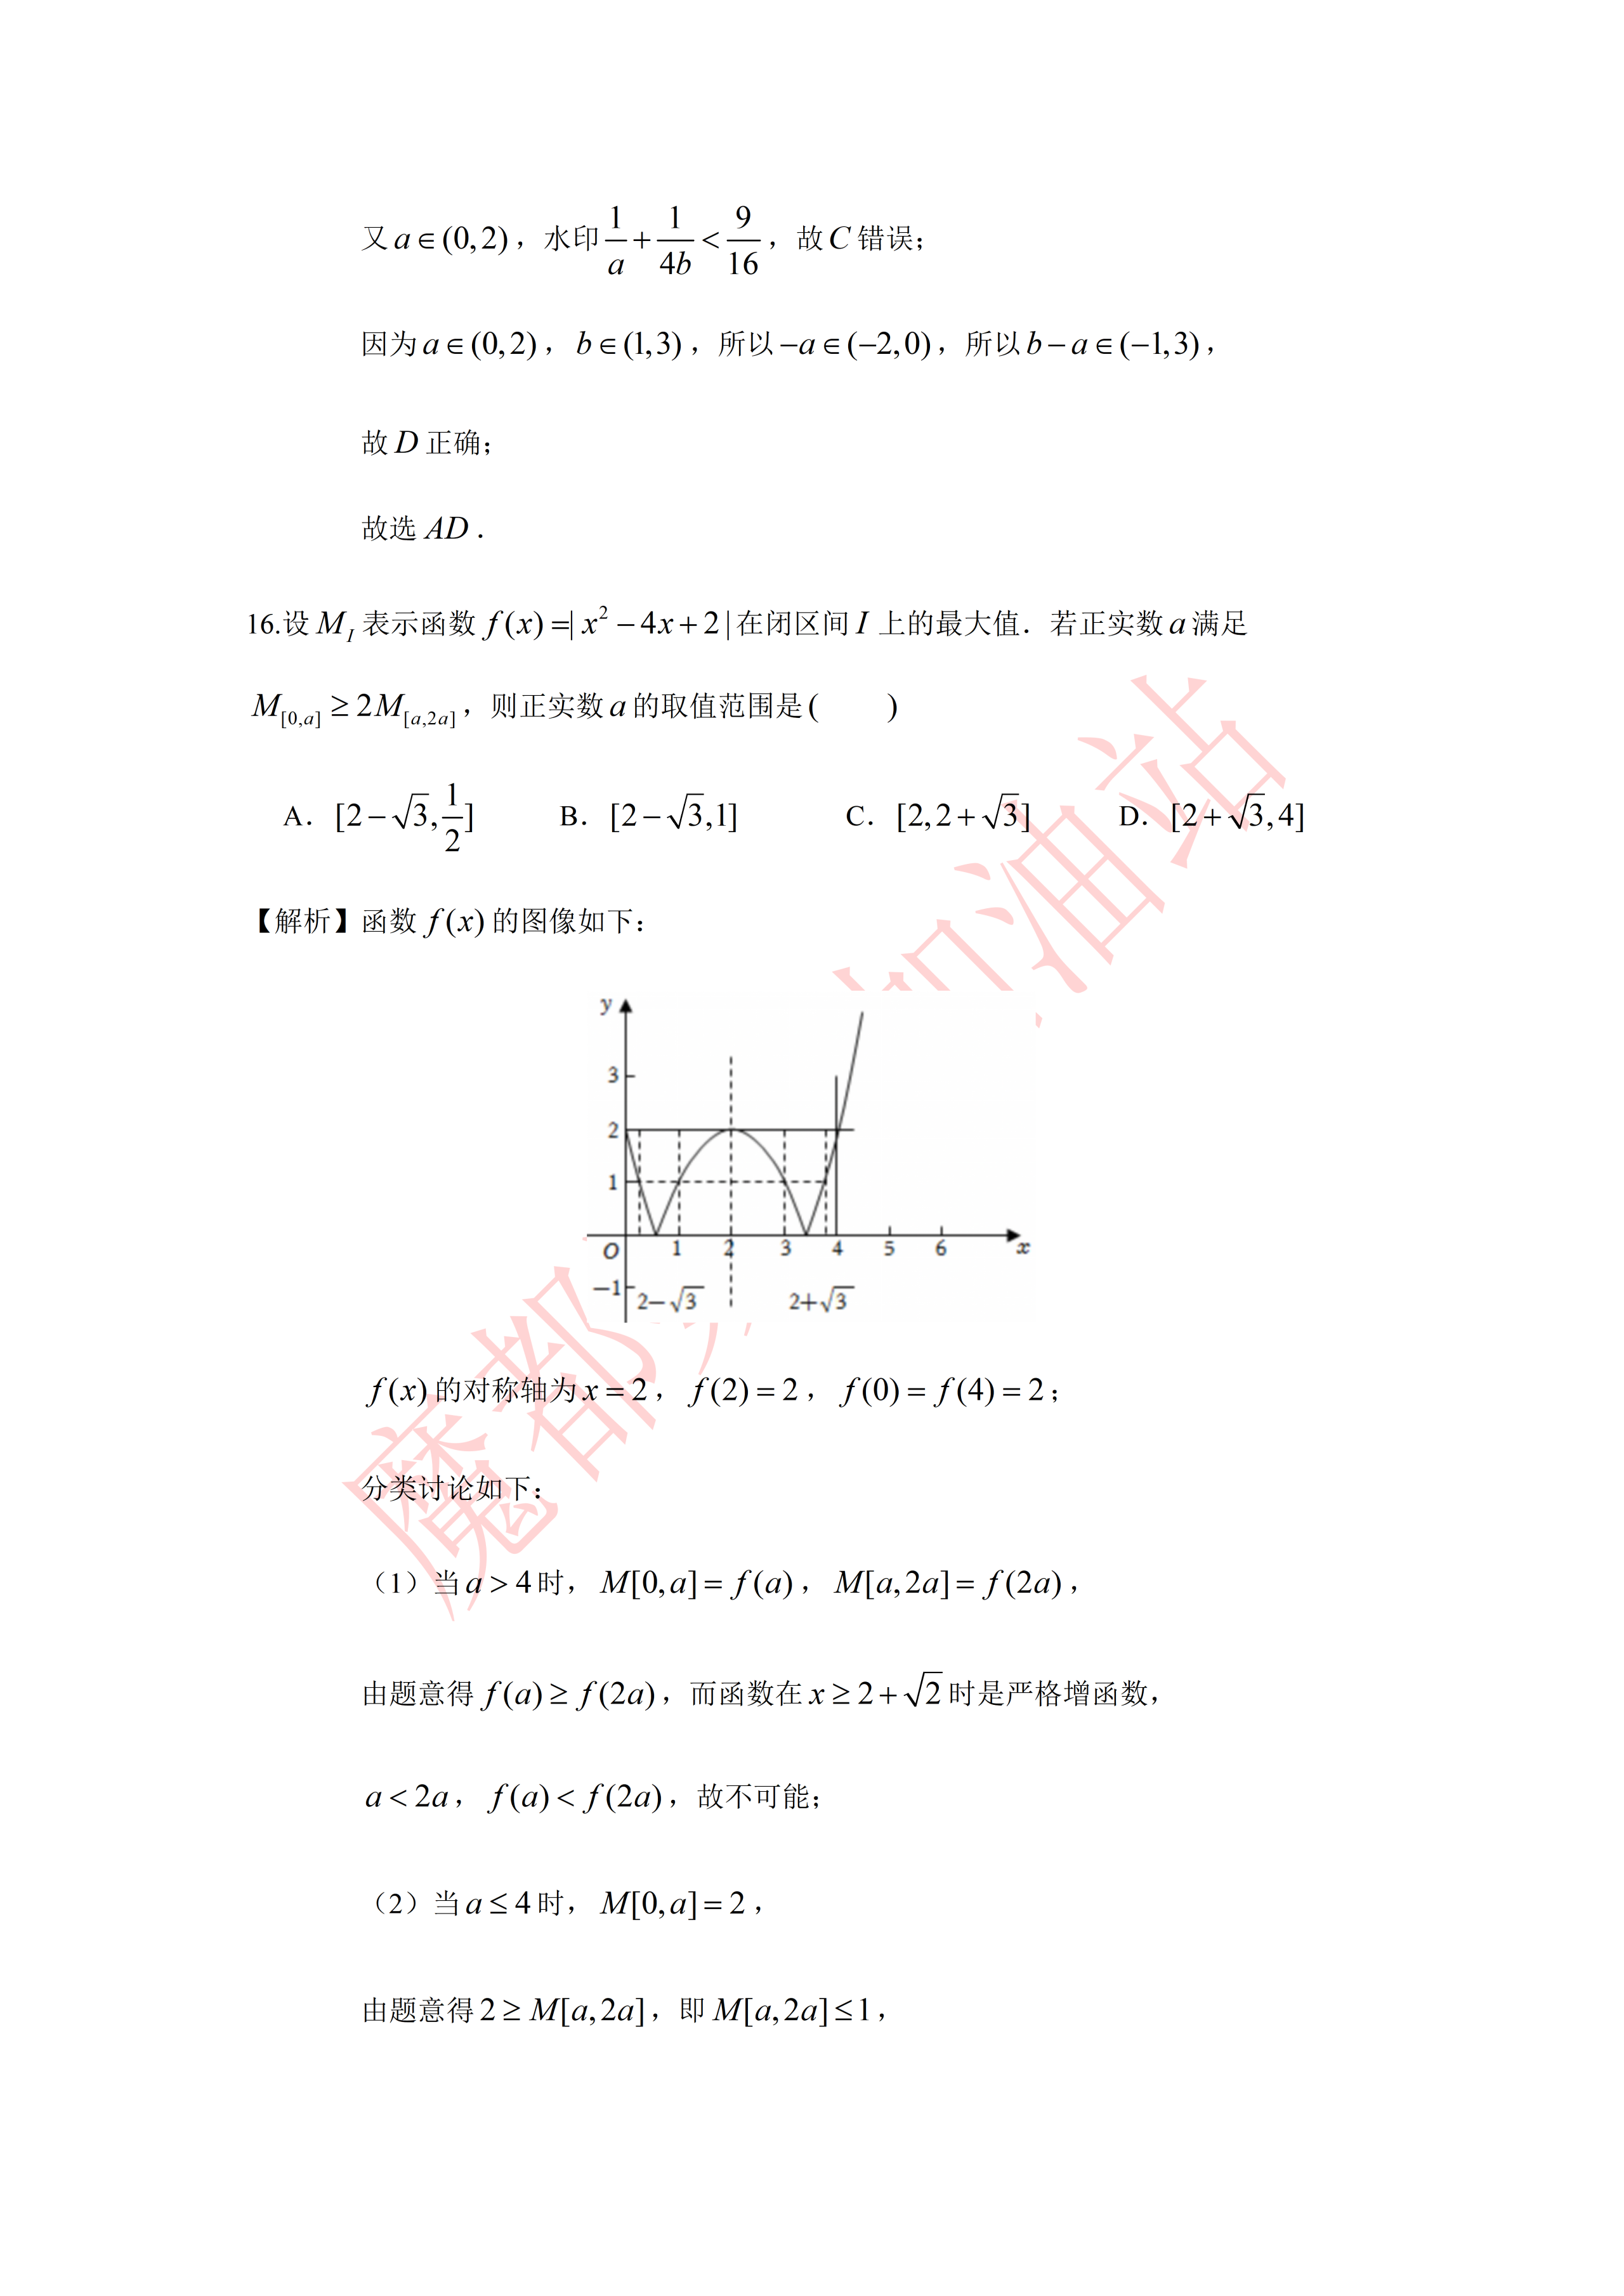
\includegraphics[width=.55\linewidth,trim=895bp 1535bp 915bp 1525bp,clip]{../原图/高一51_华师大二附中_国庆作业3/06.png}
\end{center}
\step{$f(x)$ 的对称轴为 $x=2$，$f(2)=2$，$f(0)=f(4)=2$；}
\step{分类讨论如下：}
\stepm{(1)}{当 $a>4$ 时，$M_{[0,a]}=f(a)$，$M_{[a,2a]}=f(2a)$，}
\step{由题意得 $f(a)\geqslant f(2a)$，而函数在 $x\geqslant2+\sqrt2$ 时是严格增函数，}
\step{$a<2a$，$f(a)<f(2a)$，故不可能；}
\stepm{(2)}{当 $a\leqslant4$ 时，$M_{[0,a]}=2$，}
\step{由题意得 $2\geqslant M_{[a,2a]}$，即 $M_{[a,2a]}\leqslant1$，}
\step{令 $f(x)=1$，解得 $x_1=2-\sqrt3$，$x_2=1$，$x_3=2+\sqrt3$，$x_4=3$，}
\step{则有 $a\geqslant2-\sqrt3$ 并且 $2a\leqslant1$，解得 $2-\sqrt3\leqslant a\leqslant\dfrac12$；}
\step{或者 $a\geqslant3$ 并且 $2a\leqslant2+\sqrt3$，无解；}
\step{故选 $A$.}
\solend

\fi

\end{enumerate}

\bigsec{三、解答题}

\begin{enumerate}
\setcounter{enumi}{16}

\item 已知 $M=\{x\mid2\leqslant x\leqslant5\}$，$N=\{x\mid a-1\leqslant x\leqslant2a+1\}$.
\begin{enumerate}[label=(\arabic*)]
\item 若 $M\subseteq N$，求实数 $a$ 的取值范围；
\item 若 $M\supseteq N$，求实数 $a$ 的取值范围.
\end{enumerate}

\ifanswer
\ans{（1）$[2,3]$；（2）$(-\infty,-2)$}
\fi

\ansspace[6]

\item 设集合 $A=\{x\mid|x+1|\leqslant3\}$，$B=\{x\mid0<x<3m\}$.
\begin{enumerate}[label=(\arabic*)]
\item 若 $A\cup B=A$，求实数 $m$ 的取值范围；
\item 设 $P=(\complement_R A)\cap B$，若 $\exists x\in\Z$ 且 $x\in P$，求实数 $m$ 的取值范围.
\end{enumerate}

\ifanswer
\solbegin
\stepm{(1)}{$A=\{x\mid|x+1|\leqslant3\}=\{x\mid-4\leqslant x\leqslant2\}$，且 $A\cup B=A$，所以 $B\subseteq A$.}
\step{若 $B=\varnothing$，此时 $0\geqslant3m$，解得 $m\leqslant0$；}
\step{若 $B\neq\varnothing$，此时 $0<3m$，且 $3m\leqslant2$，解得 $0<m\leqslant\dfrac23$；}
\step{则实数 $m$ 的取值范围是 $\left(-\infty,\dfrac23\right]$.}
\stepm{(2)}{因为 $\exists x\in\Z$ 且 $x\in P$，所以集合 $P$ 中至少存在一个整数.}
\step{$\complement_R A=\{x\mid x<-4\text{ 或 }x>2\}$，$B=\{x\mid0<x<3m\}$，}
\step{要使 $P=(\complement_R A)\cap B$ 中至少存在一个整数，则 $\begin{cases}3m>0\\3m>3\end{cases}$，解得 $m>1$，}
\step{则实数 $m$ 的取值范围是 $(1,+\infty)$.}
\solend

\fi

\ansspace[7]

\item 已知函数 $f(x)=x^2+(1-a)x-a(a\in\R)$.
\begin{enumerate}[label=(\arabic*)]
\item 解关于 $x$ 的不等式 $f(x)<0$；
\item 若 $\forall a\in[-1,1]$，$f(x)\geqslant0$ 恒成立，求实数 $x$ 的取值范围.
\end{enumerate}

\ifanswer
\solbegin
\stepm{(1)}{不等式 $x^2+(1-a)x-a<0$ 等价于 $(x-a)(x+1)<0$，}
\step{当 $a<-1$ 时，不等式的解集为 $(a,-1)$；}
\step{当 $a=-1$ 时，不等式的解集为 $\varnothing$；}
\step{当 $a>-1$ 时，不等式的解集为 $(-1,a)$.}
\stepm{(2)}{$x^2+(1-a)x-a=-a(x+1)+x^2+x$，}
\step{设 $g(a)=-a(x+1)+x^2+x$，$a\in[-1,1]$，}
\step{要使 $g(a)\geqslant0$ 在 $a\in[-1,1]$ 上恒成立，}
\step{只需 $\begin{cases}g(-1)\geqslant0\\g(1)\geqslant0\end{cases}$，即 $\begin{cases}x^2+2x+1\geqslant0\\x^2-1\geqslant0\end{cases}$，解得 $x\geqslant1$ 或 $x\leqslant-1$，}
\step{所以 $x$ 的取值范围为 $\{x\mid x\leqslant-1\text{ 或 }x\geqslant1\}$.}
\solend

\fi

\ansspace[7]

\item 若实数 $x$、$y$、$m$ 满足 $|x-m|>|y-m|$，则称 $x$ 比 $y$ 远离 $m$.
\begin{enumerate}[label=(\arabic*)]
\item 若 $2$ 比 $3x-4$ 远离 $1$，求 $x$ 的取值范围；
\item 设 $y=\dfrac{x+2}{x+1}$，其中 $x\in(0,\sqrt2)\cup(\sqrt2,+\infty)$，判断：$x$ 与 $y$ 哪一个更远离 $\sqrt2$？并说明理由.
\item 若 $x+y=2$，试问：$y$ 与 $x^2+y^2$ 哪一个更远离 $\dfrac12$？并说明理由.
\end{enumerate}

\ifanswer
\solbegin
\stepm{(1)}{由题意得 $|2-1|>|3x-4-1|$，所以 $|3x-5|<1$，解得 $\dfrac43<x<2$，}
\step{故 $x$ 的取值范围为 $\left(\dfrac43,2\right)$；}
\stepm{(2)}{$x$ 比 $y$ 更远离 $\sqrt2$，}
\step{理由如下：要证 $x$ 比 $y$ 更远离 $\sqrt2$，只要证 $|x-\sqrt2|>\left|\dfrac{x+2}{x+1}-\sqrt2\right|$，}
\step{即证 $|x-\sqrt2|>\left|\dfrac{(1-\sqrt2)(x-\sqrt2)}{x+1}\right|$，}
\step{因为 $x\in(0,\sqrt2)\cup(\sqrt2,+\infty)$，所以 $|x-\sqrt2|>0$，}
\step{所以只要证 $1>\dfrac{\sqrt2-1}{|x+1|}$，即证 $|x+1|>\sqrt2-1$，}
\step{因为 $x\in(0,\sqrt2)\cup(\sqrt2,+\infty)$，所以 $x+1\in(1,\sqrt2+1)\cup(\sqrt2+1,+\infty)$，}
\step{所以 $|x+1|>1>\sqrt2-1$，所以 $x$ 比 $y$ 更远离 $\sqrt2$；}
\stepm{(3)}{因为 $x^2+y^2\geqslant\dfrac{(x+y)^2}{2}=2$，当且仅当 $x=y=1$ 时等号成立，}
\step{所以 $\left|x^2+y^2-\dfrac12\right|=x^2+y^2-\dfrac12$，}
\step{从而 $\left|y-\dfrac12\right|-\left|x^2+y^2-\dfrac12\right|=\left|y-\dfrac12\right|-\left(x^2+y^2-\dfrac12\right)$，}
\step{①$y\geqslant\dfrac12$，$\left|y-\dfrac12\right|-\left|x^2+y^2-\dfrac12\right|=y-\dfrac12-\left(x^2+y^2-\dfrac12\right)=y-x^2-y^2$}
\step{$=y-(2-y)^2-y^2=-2y^2+5y-4=-2\left(y-\dfrac54\right)^2-\dfrac78<0$，}
\step{即 $\left|y-\dfrac12\right|<\left|x^2+y^2-\dfrac12\right|$；}
\step{②$y<\dfrac12$，}
\step{$\left|y-\dfrac12\right|-\left|x^2+y^2-\dfrac12\right|=\left(\dfrac12-y\right)-\left(x^2+y^2-\dfrac12\right)=-y-x^2-y^2+1$}
\step{$=-y-(2-y)^2-y^2+1=-2y^2+3y-3=-2\left(y-\dfrac34\right)^2-\dfrac{15}8<0$，}
\step{即 $\left|y-\dfrac12\right|<\left|x^2+y^2-\dfrac12\right|$；}
\step{综上，$\left|y-\dfrac12\right|<\left|x^2+y^2-\dfrac12\right|$，即 $x^2+y^2$ 比 $y$ 更远离 $\dfrac12$.}
\solend

\fi

\ansspace[9]

\item 对于非空有限整数集 $X$，$m\in\N^*$，定义 $X^m=\{x^m\mid x\in X\}$，对 $n\in\Z$，
$Y\oplus n=\{x+n\mid x\in Y\}$ 现有两个非空有限整数集 $A$、$B$，已知 $A\oplus1\subseteq B$ 且
$B^2\oplus(-4)\subseteq A$.
\begin{enumerate}[label=(\arabic*)]
\item 当 $A=\{-3,0\}$ 时求集合 $B$；
\item 证明：$A\subseteq\{-3,-2,0,1\}$；
\item 当 $A\oplus1=B$ 且 $B^2\oplus(-4)=A$ 时，任取 $a\in A$，$b\in B$ 构造函数
$f(x)=(x-a)(x-b)$ 问：当 $a$、$b$ 取何值时，$f(x)$ 的最小值最小？
\end{enumerate}

\ifanswer
\solbegin
\stepm{(1)}{因为 $A=\{-3,0\}$，$B^2\oplus(-4)\subseteq A$，}
\step{所以 $B^2\oplus(-4)$ 可能为 $\varnothing$、$\{-3\}$、$\{0\}$、$\{-3,0\}$，}
\step{当 $B^2\oplus(-4)=\varnothing$ 时 $B^2=\varnothing$，不满足非空，不合题意；}
\step{当 $B^2\oplus(-4)=\{-3\}$ 时 $B^2=\{1\}$，所以 $B=\{1,-1\}$、$\{1\}$、$\{-1\}$，}
\step{当 $B^2\oplus(-4)=\{0\}$ 时 $B^2=\{4\}$，所以 $B=\{2,-2\}$、$\{2\}$、$\{-2\}$，}
% 原卷如此，照录未改（此处作 $\{0,-3\}$，上一行同一集合作 $\{-3,0\}$）
\step{当 $B^2\oplus(-4)=\{0,-3\}$ 时 $B^2=\{4,1\}$，}
\step{所以 $B=\{1,2,-1,-2\}$、$\{2,-1,-2\}$、$\{2,1,-2\}$、$\{1,-1,-2\}$、$\{1,-1,2\}$、$\{1,2\}$、$\{-1,2\}$、$\{-1,-2\}$、$\{1,-2\}$，}
\step{又 $A\oplus1=\{-2,1\}\subseteq B$，得 $B$ 为 $\{1,-2\}$、$\{2,1,-2\}$、$\{1,-1,-2\}$、$\{1,2,-1,-2\}$.}
\stepm{(2)}{设 $x\in A$，因为 $A\oplus1\subseteq B$，所以 $x+1\in B$，}
\step{又 $B^2\oplus(-4)\subseteq A$，所以 $(x+1)^2-4\in A$，}
% 原卷如此，照录未改（此处及下文取 $x=2$ 处原卷均作 $(-4+1)^2-4=52-2a>0$）
\step{取 $x=-4$，则 $(-4+1)^2-4=52-2a>0$，$(5+1)^2-4=32\in A$，$\cdots$，}
\step{无限迭代，而 $A$ 为有限集，不合题意，舍去，即 $-4\notin A$；}
\step{取 $x=-3$，则 $(-3+1)^2-4=0\in A$，$(0+1)^2-4=-3\in A$，}
\step{得 $A$ 集合可为 $\{-3,0\}$；}
\step{取 $x=-2$，则 $(-2+1)^2-4=-3\in A$，$(-3+1)^2-4=0\in A$，}
\step{$(0+1)^2-4=-3\in A$，得 $A$ 集合可为 $\{-3,-2,0\}$；}
\step{取 $x=-1$，则 $(-1+1)^2-4=-4\in A$，又 $-4\notin A$，所以 $-1\notin A$，}
\step{取 $x=1$，则 $(1+1)^2-4=0\in A$，$(0+1)^2-4=-3\in A$，}
\step{$(-3+1)^2-4=0\in A$，得 $A$ 集合可为 $\{-3,0,1\}$，}
\step{取 $x=2$，则 $(2+1)^2-4=52-2a>0$，$(5+1)^2-4=32\in A$，$\cdots$，}
\step{无限迭代，而 $A$ 为有限集，不合题意，舍去，即 $2\notin A$，}
\step{同理当 $x<-4$ 或 $x>2$，且 $x\in\Z$ 时不符合 $A$ 为有限集，舍去；}
\step{故由上得 $A$ 集合可为 $\{-3,0\},\{-3,-2,0\},\{-3,0,1\},\{-3,-2,0,1\}$，}
\step{所以 $A\subseteq\{-3,-2,0,1\}$，}
\stepm{(3)}{当 $A\oplus1=B$ 且 $B^2\oplus(-4)=A$ 时，}
\step{设 $x\in B$，则 $x^2-4\in B^2\oplus(-4)=A$，}
% 原卷如此，照录未改（题设 $A=\{-3,0\}$，此处两个判别式取的是 $-2$ 与 $1$，均不属于 $A$）
\step{$x^2-4=-2$ 时 $x=\pm\sqrt2$，不为整数，不合题意；}
\step{$x^2-4=1$ 时 $x=\pm\sqrt5$，不为整数，不合题意；}
\step{所以 $A=\{-3,0\}$，又 $A\oplus1=B$，则 $B=\{-2,1\}$，}
\step{任取 $a\in A$，$b\in B$ 构造函数 $f(x)=(x-a)(x-b)$，}
\step{$f(x)=(x-a)(x-b)=x^2-(a+b)x+ab$}
\step{$=x^2-(a+b)x+\dfrac{(a+b)^2}{4}+ab-\dfrac{(a+b)^2}{4}$}
\step{$=\left[x-\dfrac{(a+b)}2\right]^2-\dfrac{(a-b)^2}{4}\geqslant-\dfrac{(a-b)^2}{4}$，所以 $f(x)_{min}=-\dfrac{(a-b)^2}{4}$，}
\step{又 $a\in A=\{-3,0\}$，$b\in B=\{-2,1\}$，所以 $a-b$ 的取值有 $-1,-4,2$，}
\step{所以 $f(x)_{min}=-\dfrac{(a-b)^2}{4}\geqslant-\dfrac{(-3-1)^2}{4}=-4$，}
\step{即当 $a=-3$，$b=1$ 时 $f(x)_{min}$ 的最小值为 $-4$.}
\solend

\fi

\ansspace*[12]

\end{enumerate}

\end{document}
"
% 紧凑版：xelatex "\def\iscompact{1}% 高一51_华师大二附中_国庆作业3.tex
%   —— 高一上数学“2026-2027 年华师大二附中高一上国庆作业 3”（讲评版）
% 试卷版：xelatex 高一51_华师大二附中_国庆作业3.tex
% 答案版：xelatex "\def\isanswer{1}% 高一51_华师大二附中_国庆作业3.tex
%   —— 高一上数学“2026-2027 年华师大二附中高一上国庆作业 3”（讲评版）
% 试卷版：xelatex 高一51_华师大二附中_国庆作业3.tex
% 答案版：xelatex "\def\isanswer{1}\input{高一51_华师大二附中_国庆作业3.tex}"
% 紧凑版：xelatex "\def\iscompact{1}\input{高一51_华师大二附中_国庆作业3.tex}"
%
% 原始材料：微信公众号“魔都数学加油站”文章，作者破晓，连载“27学年高一51”；
% 原文标题“27学年高一51——2026-2027年上海市华师大二附中高一上国庆作业3”；
% 原文链接：https://mp.weixin.qq.com/s/95SLMEmPUT30s4U7wjr5Og。
% 该页面用 JS 渲染，未见明确发布日期；页面内时间戳约为 2026-10-05 21:37，本稿以该时刻记可得日期。
% 正文为 12 张 PNG 页：第 01、02、03、05、07、08、11 页 4762×6735，
% 第 04、06、09、10、12 页 2560×3620。按页序逐页读取，12 页全为试卷正文页
% （卷首标题在第 1 页页顶，卷末解答题止于第 12 页），无封面页、目录页或单独的页脚页。
% 卷面标题照原卷印作“2026-2027 年华师大二附中高一上国庆作业 3”（公众号标题中的“上海市”
% 卷面标题行没有，本稿照卷面），年份区间按全稿惯例排 en dash。
%
% 篇幅与题号：原卷自第 3 题起编号（第 1、2 题不在本卷内）。填空题 3—12（10 题）、
% 选择题 13—16（4 题）、解答题 17—21（5 题），共 19 题。本稿沿用原节与原题号，
% 只改排为全稿统一的大节样式（原卷小节标题为“一、填空题”“二、选择题”“三、解答题”）。
% 正文为讲评版：填空题 3—12 与选择题 13—16 只印【解析】（选择题的结论“故选 X”印在解析内），
% 按全稿口径这类题不另提 \ans{}；解答题第 17 题只印【答案】，故只给 \ans{}；
% 第 18—21 题只印【解析】。
%
% 副标题：原卷未印副标题。本稿按“知识模块”口径标作“集合与常用逻辑用语、不等式”：
% 19 题中集合与常用逻辑用语 8 题（3、4、6、10、13、17、18、21），
% 不等式（含函数最值、绝对值不等式）11 题（5、7、8、9、11、12、14、15、16、19、20），
% 两类均远超三分之一，故并标。口径同 高一46_交附闵行_国庆作业3、高一48_华师大二附中_周末作业2。
%
% 与原卷的排版差异：
%   ① 原卷每题下直接印【答案】或【解析】，本稿按全稿惯例将答案与解析置于答案版；
%   ② 原卷未印副标题，本稿按“知识模块”口径补出；
%   ③ 原卷填空横线按全稿惯例排为 \blankline[4.4em]；
%   ④ 原卷 $R$、$N$、$Z$ 均排斜体，本稿按全稿惯例改用花体 $\R$、$\N$、$\Z$（同 高一48）；
%   ⑤ 原卷第 12 题解析配图、第 13 题题干韦恩图都印在正文右侧的浮动位置，第 16 题解析配图
%      印在解析行间；本稿三图一律居中排，均自原图对应页裁切（trim），不另存图片文件；
%   ⑥ 原卷解答题未留作答空白，本稿按全稿惯例加 \ansspace；
%   ⑦ 原卷第 15 题解析第 7、8 两个印刷行是一串连等式的折行，本稿按“一条 \step ＝ 一个印刷行”
%      的口径分成两条 \step。
%
% 原卷笔误/存疑（均照录未改，正文对应处另有 % 注）：
%   ① 第 12 题解析末行作“区间长度之和为 $x_1-b+x_2-a=x_1-x_2-a-b=2+a+b-a-b=2$”，
%      按上一行 $x_1+x_2=2+a+b$，此处应为 $x_1+x_2$；原卷作 $x_1-x_2$。
%   ② 第 15 题解析“又 $a\in(0,2)$，”与 $\dfrac1a+\dfrac1{4b}<\dfrac9{16}$ 之间，
%      原卷正文夹印“水印”二字（系制版遗留字样，非试卷内容）。
%   ③ 第 21 题第 (2) 问解析两处（取 $x=-4$、取 $x=2$）作“$=52-2a>0$”，
%      与题设 $(x+1)^2-4$ 的取值（按 $x=-4$ 应为 $5$）不符，当系原卷算式遗留。
%   ④ 第 21 题第 (1) 问解析先写 $B^2\oplus(-4)$ 可能为 $\{-3,0\}$，后文又作 $\{0,-3\}$，
%      同一集合两种写法。
%   ⑤ 第 21 题第 (3) 问解析：题设 $B^2\oplus(-4)=A$ 且 $A=\{-3,0\}$ 时，由 $x^2-4\in A$
%      应得 $x^2-4=-3$ 或 $0$；原卷讨论的却是 $x^2-4=-2$ 与 $x^2-4=1$（两值均不属于 $A$），
%      与题设不合。
%
% 插图：3 张，均自原图裁切（无 \begin{tikzpicture} 重排）：
%   · 第 13 题题干韦恩图（原图第 04 页，图在题干与选项右侧）
%   · 第 12 题解析配图（原图第 04 页，图在解析右侧）
%   · 第 16 题解析配图（原图第 06 页，图在解析中间）
%
\documentclass[a4paper,11pt]{article}
\usepackage{common}

\begin{document}

\examtitlest[3]{2026--2027 年华师大二附中高一上国庆作业 3}{集合与常用逻辑用语、不等式}

\bigsec{一、填空题}

\begin{enumerate}
\setcounter{enumi}{2}

\item 若 $\{x\mid x<1\text{ 或 }x>4\}\cup\{x\mid m<x<2m+3\}=R$，则实数 $m$ 的取值范围为\blankline[4.4em].

\ifanswer
\solbegin
\step{因为 $\{x\mid x<1\text{ 或 }x>4\}\cup\{x\mid m<x<2m+3\}=R$，}
\step{所以 $\begin{cases}m<1\\2m+3>4\end{cases}$，解得 $\dfrac12<m<1$，所以 $m$ 的取值范围为 $\left(\dfrac12,1\right)$.}
\solend

\fi

\item 若“$x\leqslant5$”是“$x<a$”的必要不充分条件，则 $a$ 的取值范围是\blankline[4.4em].

\ifanswer
\solbegin
\step{若“$x\leqslant5$”是“$x<a$”的必要不充分条件，则 $\{x\mid x<a\}\subset\{x\mid x\leqslant5\}$，}
\step{所以 $a\leqslant5$.}
\solend

\fi

\item 实数 $x$、$y$ 满足 $x^2+2xy+4y^2=1$，则 $x+2y$ 的取值范围是\blankline[4.4em].

\ifanswer
\solbegin
\step{因为 $x^2+2xy+4y^2=(x+2y)^2-2xy=1$，}
\step{所以 $(x+2y)^2-1=x\cdot(2y)\leqslant\left(\dfrac{x+2y}{2}\right)^2$，当且仅当 $x=2y$ 时取等号，}
\step{解得 $-\dfrac{2\sqrt3}{3}\leqslant x+2y\leqslant\dfrac{2\sqrt3}{3}$，故 $x+2y$ 的取值范围是 $\left[-\dfrac{2\sqrt3}{3},\dfrac{2\sqrt3}{3}\right]$.}
\solend

\fi

\item 若命题 $p$：“$\exists x\in\R$，$5x^2-3x+m=0$”为假命题，则实数 $m$ 的取值范围为\blankline[4.4em].

\ifanswer
\solbegin
\step{若命题 $p$：$\exists x\in\R$，$5x^2-3x+m=0$ 为假命题，}
\step{则 $5x^2-3x+m=0$ 没有实数根，故 $\Delta=9-20m<0$，解得 $m>\dfrac9{20}$.}
\solend

\fi

\item 若当 $3\leqslant m\leqslant5$ 时，$mx^2-mx+m-9<0$ 有解，则实数 $x$ 的取值范围是\blankline[4.4em].

\ifanswer
\solbegin
\step{当 $3\leqslant m\leqslant5$ 时，$mx^2-mx+m-9<0$ 有解，}
\step{即 $(x^2-x+1)m-9<0$ 在 $m\in[3,5]$ 上有解，}
\step{因为 $x^2-x+1>0$，所以一次函数 $g(m)=(x^2-x+1)m-9$ 严格增，}
\step{所以只需 $g(3)=3x^2-3x-6<0$ 即可，}
\step{即 $x^2-x-2<0$，$(x-2)(x+1)<0$，解得 $-1<x<2$，}
\step{所以实数 $x$ 的取值范围是 $(-1,2)$.}
\solend

\fi

\item 已知不等式 $\dfrac{x}{x^2+4}\leqslant a$ 对任意的 $x\in[1,3]$ 恒成立，则实数 $a$ 的范围为\blankline[4.4em].

\ifanswer
\solbegin
\step{因为 $x\in[1,3]$，所以 $\dfrac{x}{x^2+4}=\dfrac{1}{x+\dfrac4x}\leqslant\dfrac{1}{2\sqrt{x\times\dfrac4x}}=\dfrac14$，}
\step{当且仅当 $x=\dfrac4x$ 时，即 $x=2$ 时取等号，即 $\dfrac{x}{x^2+4}$ 在 $x\in[1,3]$ 的最大值为 $\dfrac14$，}
\step{又由不等式 $\dfrac{x}{x^2+4}\leqslant a$ 对任意的 $x\in[1,3]$ 恒成立，所以 $a\geqslant\dfrac14$，}
\step{即实数 $a$ 的范围为 $\left[\dfrac14,+\infty\right)$.}
\solend

\fi

\item 甲、乙两人解关于 $x$ 的不等式 $x^2+bx+c<0$，甲写错了 $b$，正确计算后得到的解为 $\{x\mid1<x<2\}$；
乙写错了 $c$，正确计算后得到的解为 $\{x\mid-4<x<1\}$. 那么不等式 $\dfrac{bx+c}{x-2}<0$ 的解为\blankline[4.4em].

\ifanswer
\solbegin
\step{由 $x^2+bx+c<0$ 的解为 $\{x\mid1<x<2\}$，}
\step{则 $1$ 和 $2$ 是方程 $x^2+bx+c=0$ 的两个根，}
\step{甲写错了 $b$，但 $c$ 是正确的，所以 $c=1\times2=2$；}
\step{由 $x^2+bx+c<0$ 的解为 $\{x\mid-4<x<1\}$，}
\step{则 $-4$ 和 $1$ 是方程 $x^2+bx+c=0$ 的两个根，}
\step{乙写错了 $c$，但 $b$ 是正确的，所以 $-b=-4+1=-3$，即 $b=3$.}
\step{由 $\dfrac{bx+c}{x-2}<0$，得 $\dfrac{3x+2}{x-2}<0$，即 $(3x+2)(x-2)<0$，解得 $-\dfrac23<x<2$.}
\step{不等式 $\dfrac{bx+c}{x-2}<0$ 的解为 $\left\{x\mid-\dfrac23<x<2\right\}$.}
\solend

\fi

\item 已知 $\dfrac{1}{x-2}\geqslant1$ 是 $|x-a|<2$ 的充分非必要条件，则实数 $a$ 的取值范围是\blankline[4.4em].

\ifanswer
\solbegin
\step{由 $\dfrac{1}{x-2}\geqslant1$ 得 $\dfrac{3-x}{x-2}\geqslant0$，解得 $2<x\leqslant3$，由 $|x-a|<2$ 得 $a-2<x<a+2$，}
\step{因为 $\dfrac{1}{x-2}\geqslant1$ 是 $|x-a|<2$ 的充分非必要条件，}
\step{所以 $\{x\mid2<x\leqslant3\}\subset\{x\mid a-2<x<a+2\}$，所以 $\begin{cases}a-2\leqslant2\\a+2>3\end{cases}$，解得 $1<a\leqslant4$，}
\step{即实数 $a$ 的取值范围是 $(1,4]$.}
\solend

\fi

\item 设 $a>0$，$b>0$，若不等式 $a(a+1)^2+b(b+1)^2\geqslant\lambda ab$ 恒成立，则实数 $\lambda$ 的最大值为\blankline[4.4em].

\ifanswer
\solbegin
\step{$a(a+1)^2+b(b+1)^2\geqslant\lambda ab\Leftrightarrow\lambda\leqslant\dfrac{a(a+1)^2+b(b+1)^2}{ab}=\dfrac{(a+1)^2}{b}+\dfrac{(b+1)^2}{a}$，}
\step{从而原问题转化为求 $\dfrac{(a+1)^2}{b}+\dfrac{(b+1)^2}{a}$ 的最小值.}
\step{因为 $\dfrac{(a+1)^2}{b}+\dfrac{(b+1)^2}{a}=\dfrac{b^2+2b+1}{a}+\dfrac{a^2+2a+1}{b}$}
\step{$=\left(\dfrac{b^2}{a}+\dfrac{a^2}{b}\right)+2\left(\dfrac ba+\dfrac ab\right)+\left(\dfrac1a+\dfrac1b\right)\geqslant2\sqrt{\dfrac{b^2}{a}\cdot\dfrac{a^2}{b}}+2\times2\sqrt{\dfrac ba\cdot\dfrac ab}+2\sqrt{\dfrac1a\cdot\dfrac1b}$}
\step{$=2\sqrt{ab}+4+\dfrac{2}{\sqrt{ab}}\geqslant2\sqrt{2\sqrt{ab}\cdot\dfrac{2}{\sqrt{ab}}}+4=8$，以上均当且仅当 $a=b$ 时取等号，}
\step{所以 $\lambda\leqslant8$，即实数 $\lambda$ 的最大值为 $8$.}
\solend

\fi

\item 定义区间 $(a,d)$、$[a,d)$、$(a,d]$、$[a,d]$ 的长度为 $d-a$（$d>a$），已知 $a>b$，则满足
$\dfrac{1}{x-a}+\dfrac{1}{x-b}\geqslant1$ 的 $x$ 构成的区间的长度之和为\blankline[4.4em].

\ifanswer
\solbegin
\step{因为 $\dfrac{1}{x-a}+\dfrac{1}{x-b}\geqslant1$，所以 $\dfrac{2x-(a+b)}{(x-a)(x-b)}\geqslant1$，}
\step{即 $\dfrac{2x-(a+b)}{(x-a)(x-b)}-1\geqslant0$，则 $\dfrac{x^2-(2+a+b)x+ab+a+b}{(x-a)(x-b)}\leqslant0$，}
\step{设 $x^2-(2+a+b)x+ab+a+b=0$ 的根为 $x_1$ 和 $x_2$，}
\begin{center}
% 原卷该图印在解析右侧（原图第 04 页），本稿移作居中排，直接裁取原图，不另存图片文件。
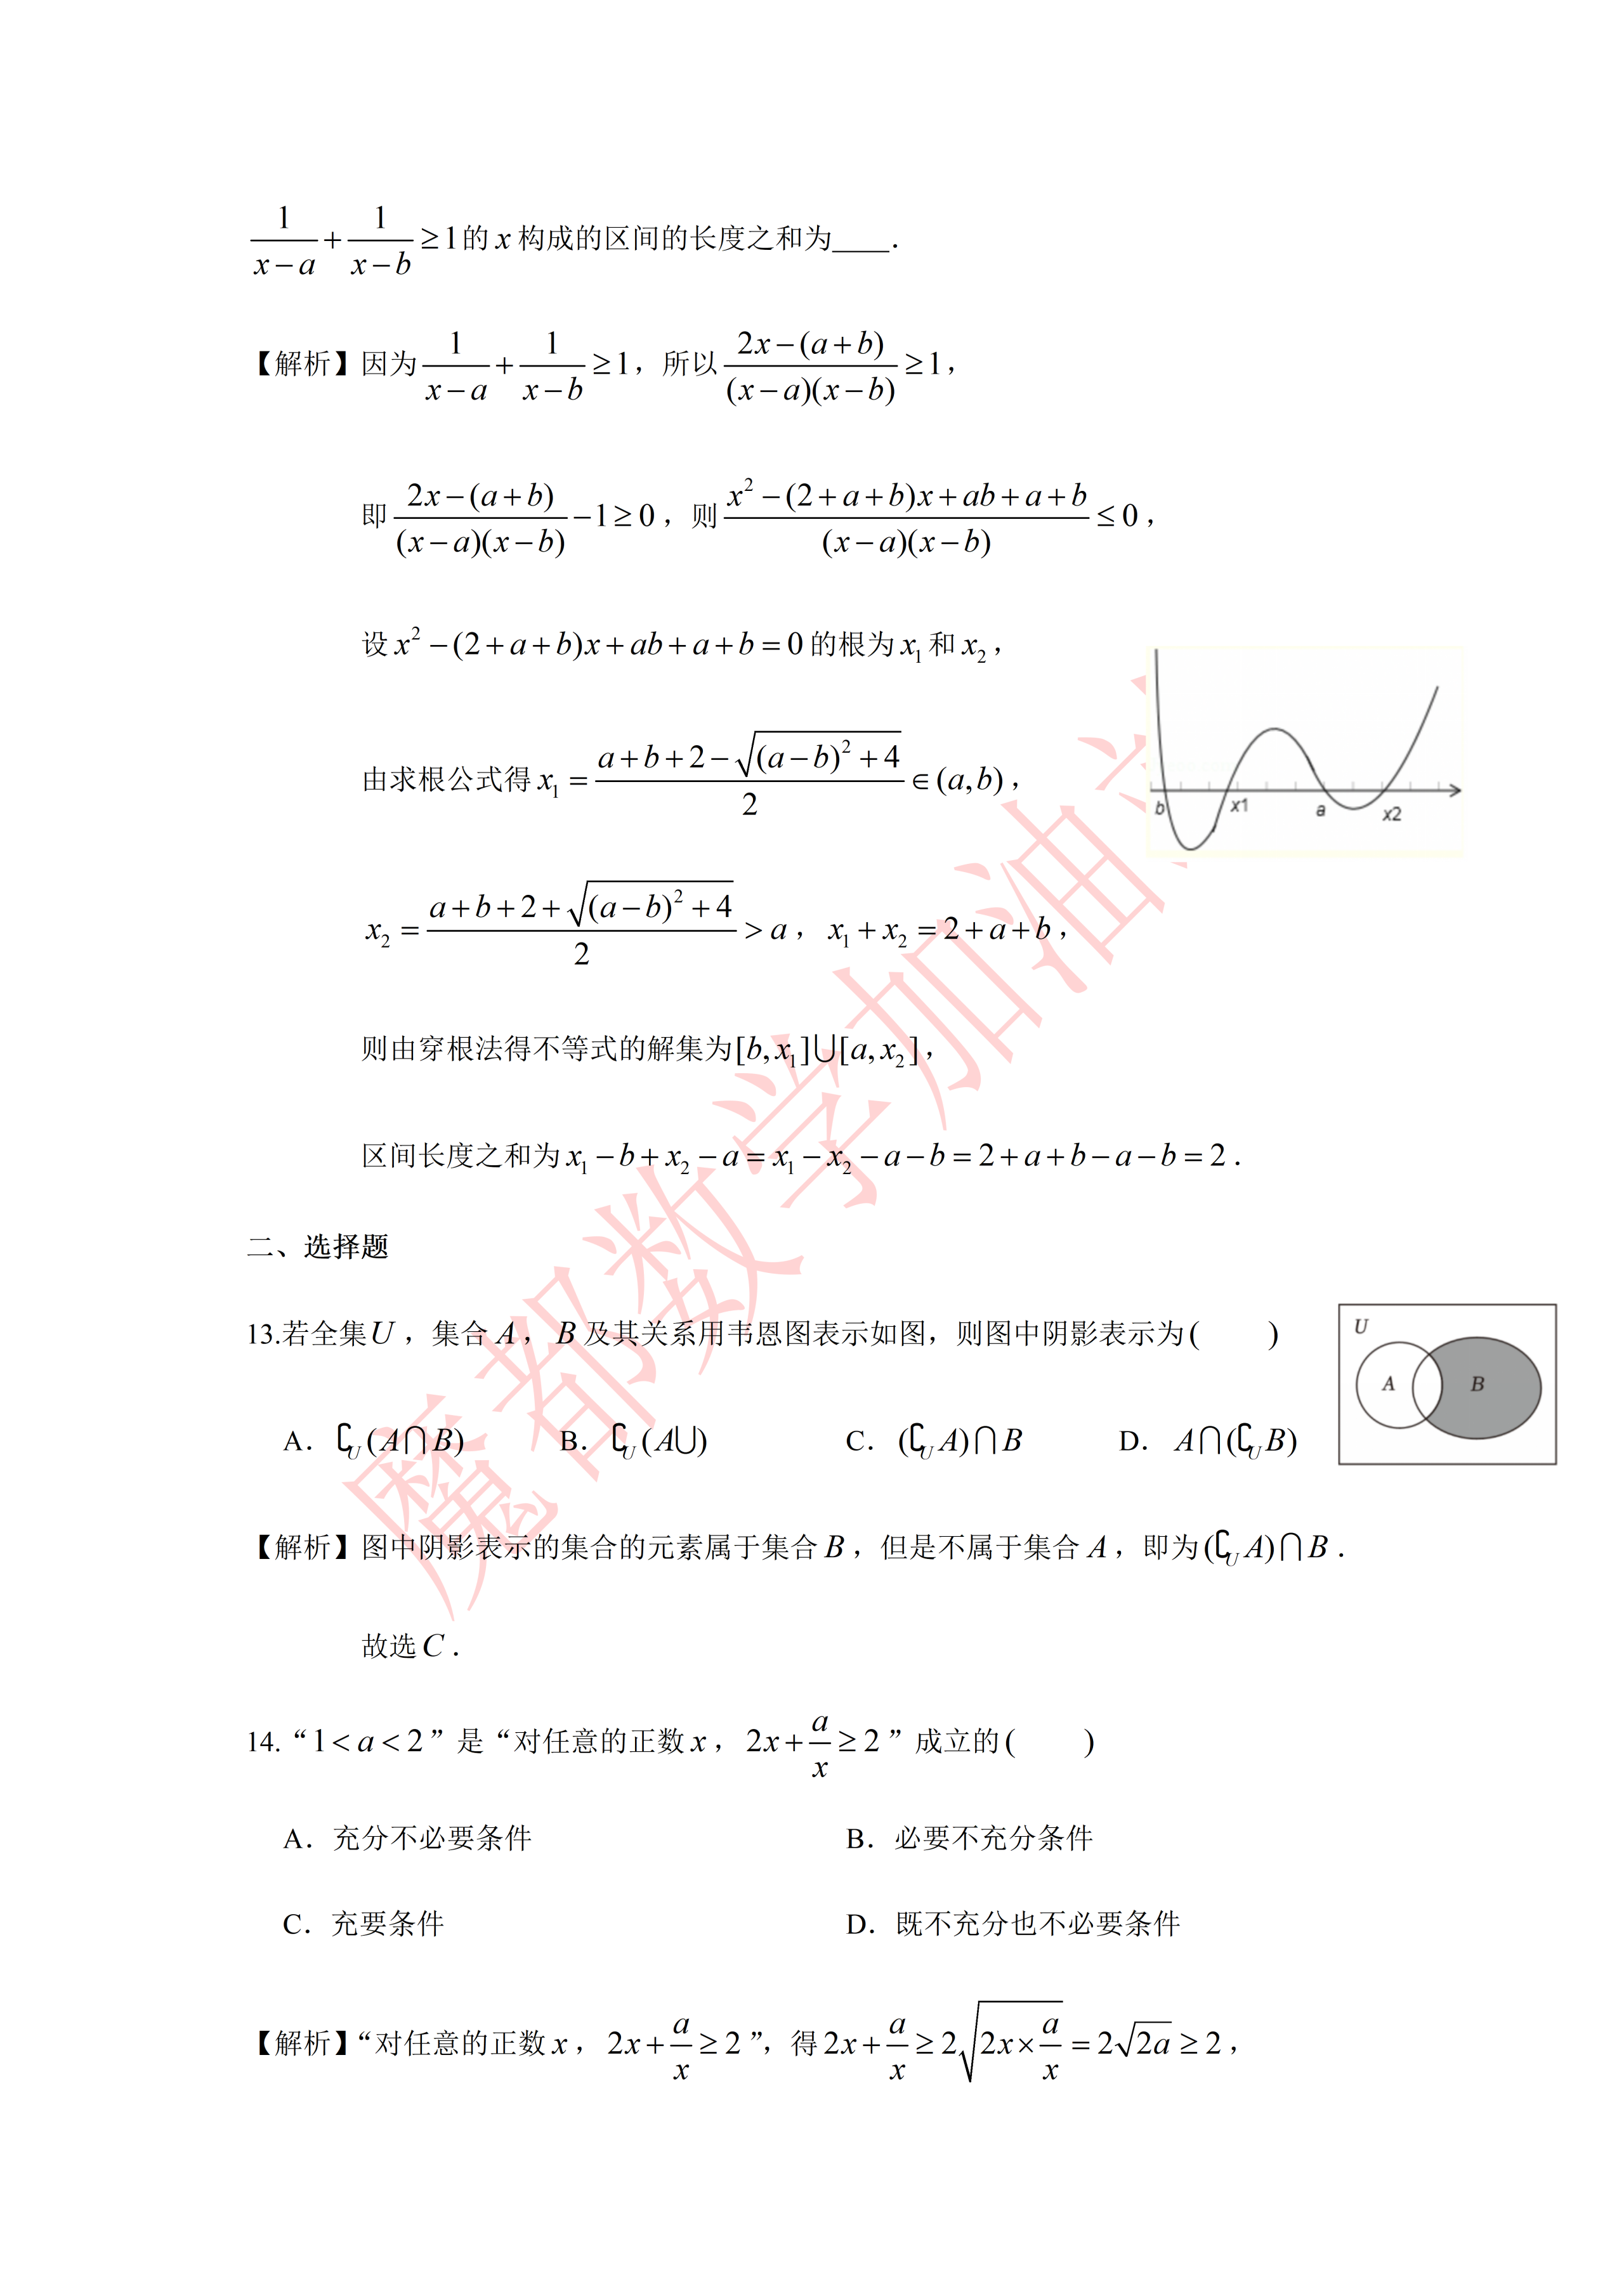
\includegraphics[width=.50\linewidth,trim=1786bp 2255bp 228bp 985bp,clip]{../原图/高一51_华师大二附中_国庆作业3/04.png}
\end{center}
\step{由求根公式得 $x_1=\dfrac{a+b+2-\sqrt{(a-b)^2+4}}{2}\in(a,b)$，}
\step{$x_2=\dfrac{a+b+2+\sqrt{(a-b)^2+4}}{2}>a$，$x_1+x_2=2+a+b$，}
\step{则由穿根法得不等式的解集为 $[b,x_1]\cup[a,x_2]$，}
% 原卷如此，照录未改（此处原卷作 $x_1-x_2$，按上一行 $x_1+x_2=2+a+b$ 当为 $x_1+x_2$）
\step{区间长度之和为 $x_1-b+x_2-a=x_1-x_2-a-b=2+a+b-a-b=2$.}
\solend

\fi

\end{enumerate}

\bigsec{二、选择题}

\begin{enumerate}
\setcounter{enumi}{12}

% 本题是“题干 + 图 + 选项”约 5.5cm 的一整块，图夹在题干与选项之间时 \keepwithprev 挡不住断点，
% 故按 高一30 第 13 题的成例在题前先量一次页高（守卫放在 \item 之前）。
\needvspace{6cm}
\item 若全集 $U$，集合 $A$、$B$ 及其关系用韦恩图表示如图，则图中阴影表示为\mbox{（\quad）}

\begin{center}
% 原卷该图印在题干与选项右侧（原图第 04 页），本稿移作居中排，直接裁取原图，不另存图片文件。
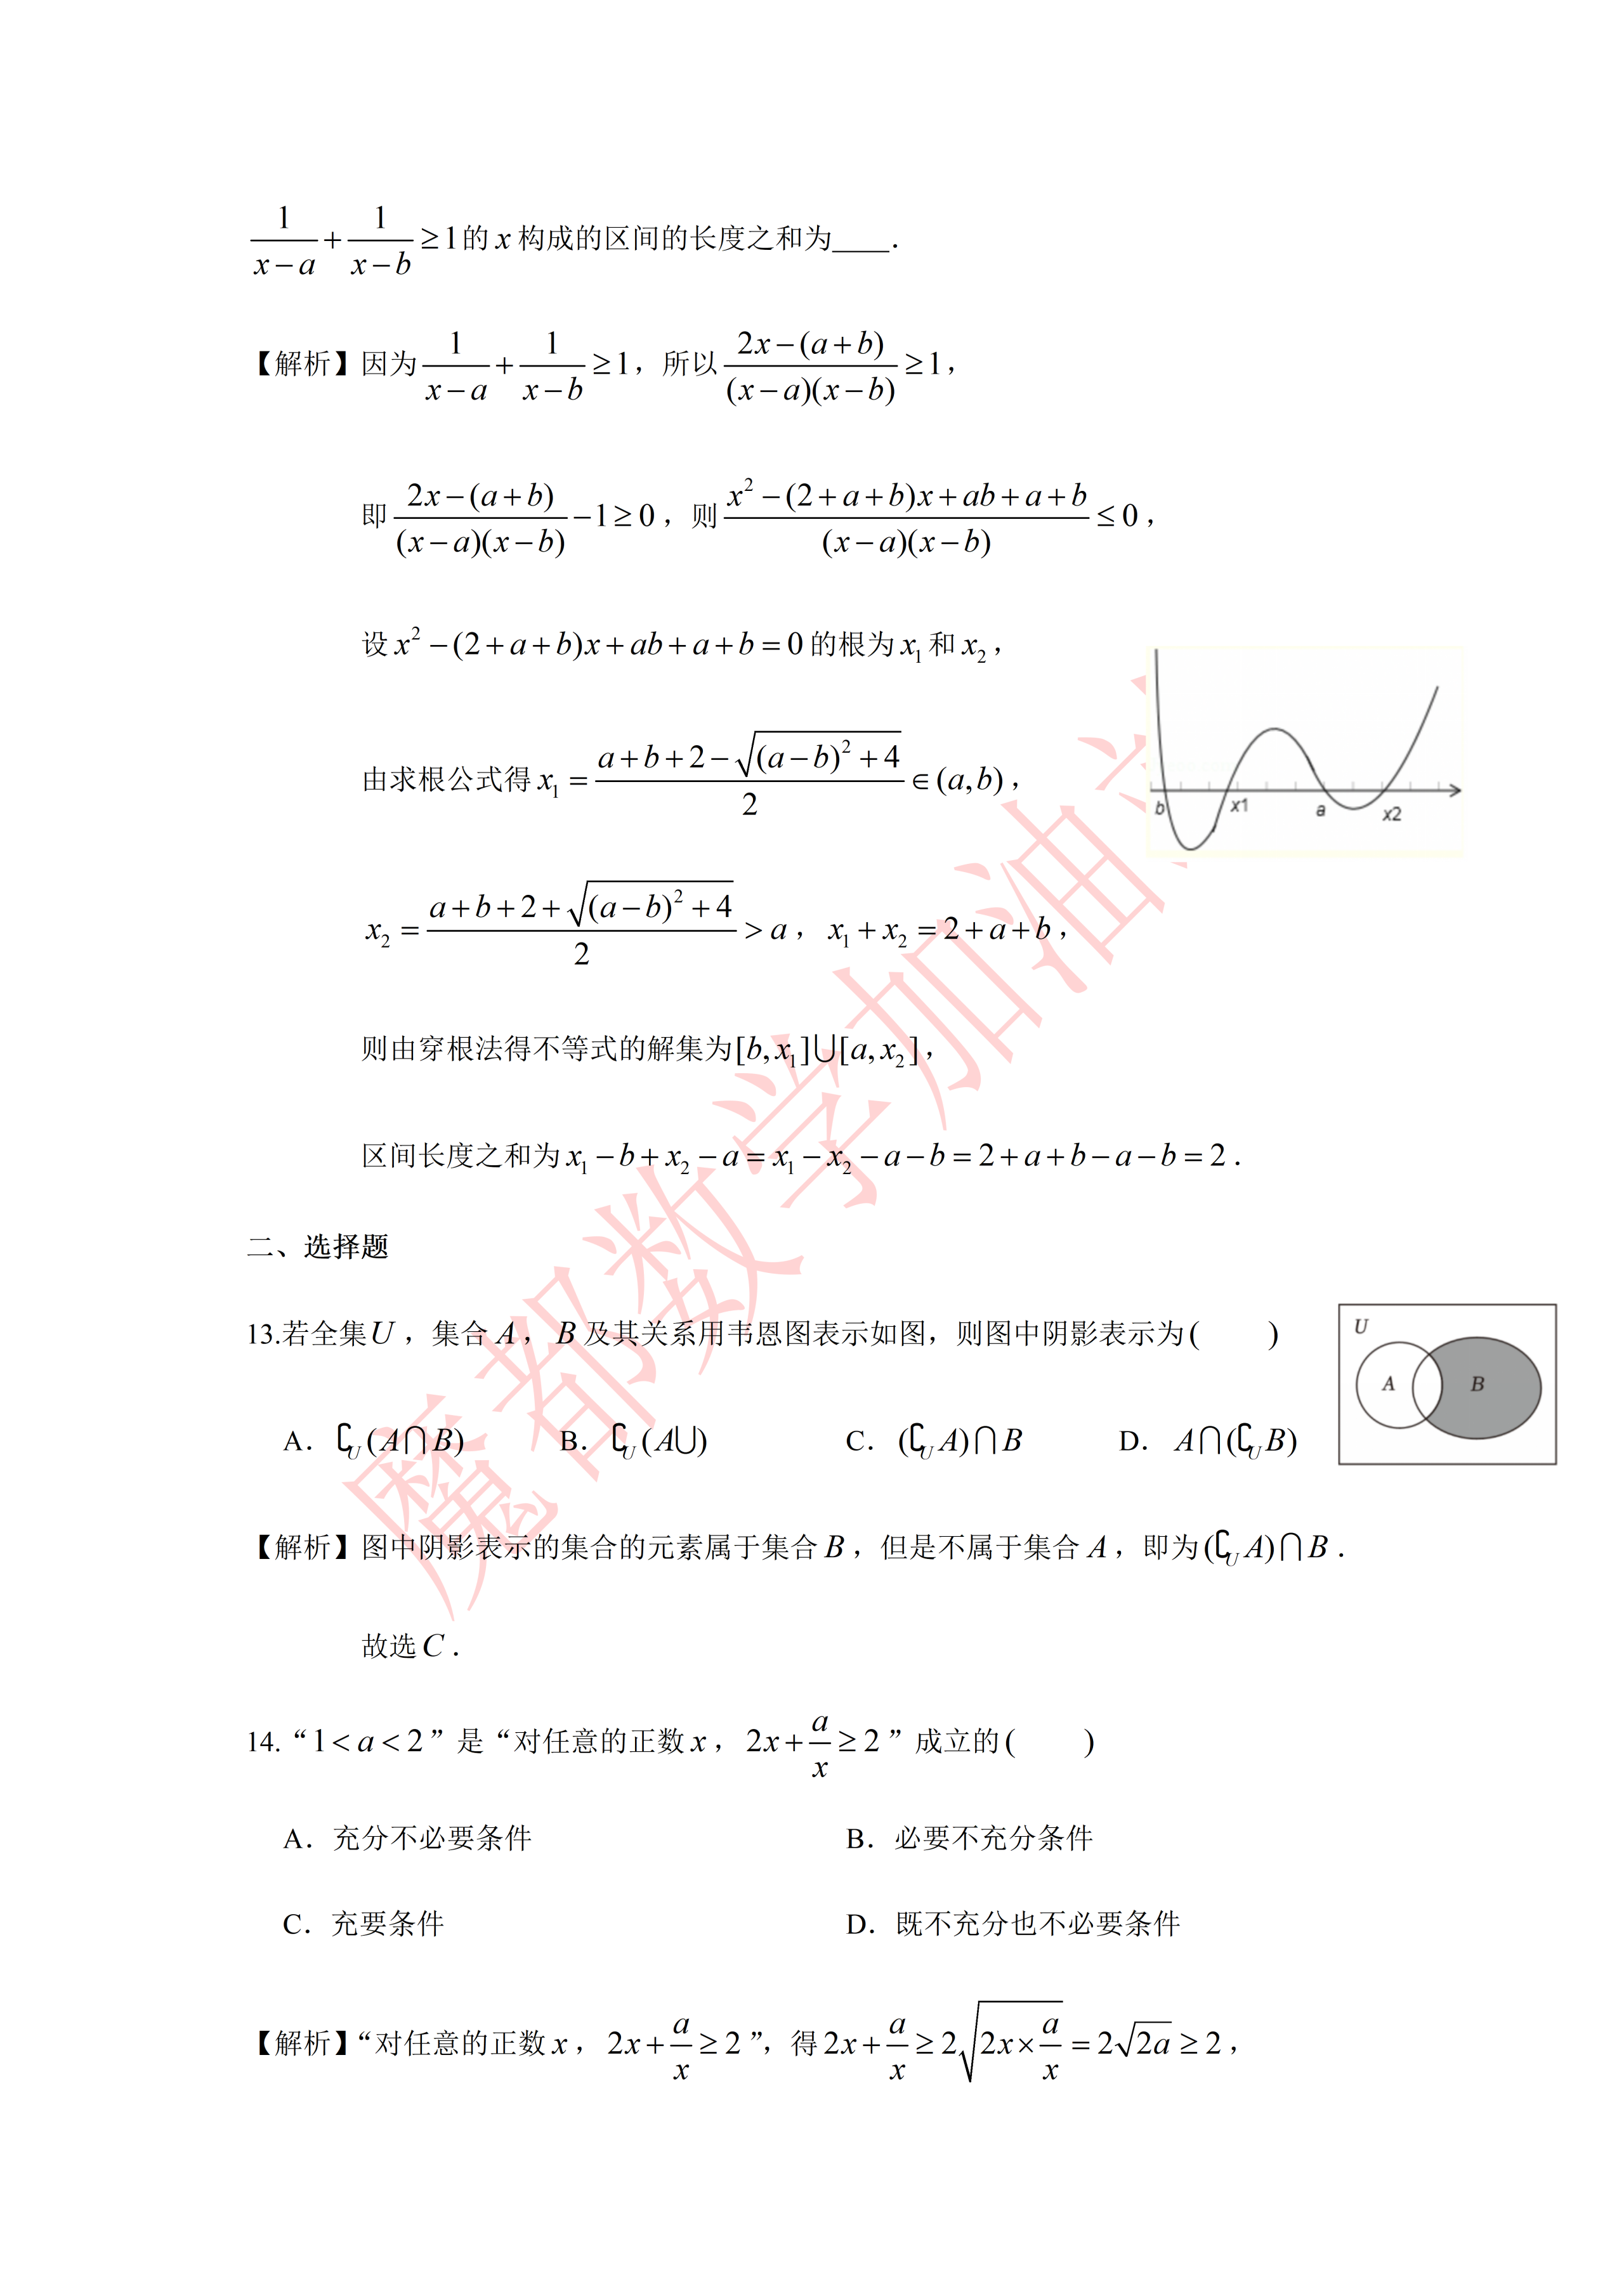
\includegraphics[width=.30\linewidth,trim=2105bp 1308bp 105bp 2050bp,clip]{../原图/高一51_华师大二附中_国庆作业3/04.png}
\end{center}

\keepwithprev
A. $\complement_U(A\cap B)$\qquad B. $\complement_U(A\cup B)$

C. $(\complement_U A)\cap B$\qquad D. $A\cap(\complement_U B)$

\ifanswer
\solbegin
\step{图中阴影表示的集合的元素属于集合 $B$，但是不属于集合 $A$，即为 $(\complement_U A)\cap B$.}
\step{故选 $C$.}
\solend

\fi

\item “$1<a<2$”是“对任意的正数 $x$，$2x+\dfrac ax\geqslant2$”成立的\mbox{（\quad）}

\keepwithprev
A. 充分不必要条件\qquad B. 必要不充分条件

C. 充要条件\qquad\qquad D. 既不充分也不必要条件

\ifanswer
\solbegin
\step{“对任意的正数 $x$，$2x+\dfrac ax\geqslant2$”，得 $2x+\dfrac ax\geqslant2\sqrt{2x\times\dfrac ax}=2\sqrt{2a}\geqslant2$，}
\step{所以 $\sqrt{2a}\geqslant1$，解得 $a\geqslant\dfrac12$，}
\step{若“$1<a<2$”得 $2x+\dfrac ax\geqslant2\sqrt{2x\times\dfrac ax}=2\sqrt{2a}>2\sqrt2>2$，}
\step{所以“$1<a<2$”$\Rightarrow$“对任意的正数 $x$，$2x+\dfrac ax\geqslant2$”，}
\step{所以“$1<a<2$”是“对任意的正数 $x$，$2x+\dfrac ax\geqslant2$”成立的充分不必要条件，}
\step{故选 $A$.}
\solend

\fi

\item 已知函数 $f(x)=2x-3$，$x\in(0,2)$，实数 $a$、$b$ 满足 $f(a)+f(b-1)=0$，则以下成立的有\mbox{（\quad）}

\keepwithprev
A. $a(b-1)$ 的最大值为 $\dfrac94$\qquad\qquad B. $b-\dfrac1a$ 的最大值为 $2$

C. $\dfrac1a+\dfrac1{4b}$ 的最小值为 $\dfrac9{16}$\qquad D. $-1<b-a<3$

\ifanswer
\solbegin
\step{因为函数 $f(x)=2x-3$，$x\in(0,2)$，实数 $a$、$b$ 满足 $f(a)+f(b-1)=0$，}
\step{所以 $2a-3+2(b-1)-3=0$，得 $a+b=4$，$a\in(0,2)$，$b\in(1,3)$，}
\step{所以 $a(b-1)=a(3-a)=-\left(a-\dfrac32\right)^2+\dfrac94$，$a\in(0,2)$，}
\step{所以 $0<a(b-1)\leqslant\dfrac94$，故选项 $A$ 正确；}
\step{$b-\dfrac1a=4-a-\dfrac1a=4-\left(a+\dfrac1a\right)\leqslant4-2=2$，}
\step{当且仅当 $a=1$，$b=3$ 时取等号，又 $b\in(1,3)$，故 $b-\dfrac1a<2$，故 $B$ 错误；}
\step{$\dfrac1a+\dfrac1{4b}=\dfrac14\left(\dfrac1a+\dfrac1{4b}\right)(a+b)=\dfrac14\left(1+\dfrac14+\dfrac ba+\dfrac a{4b}\right)=\dfrac5{16}+\dfrac14\left(\dfrac ba+\dfrac a{4b}\right)$}
\step{$\geqslant\dfrac5{16}+\dfrac14\cdot2\sqrt{\dfrac ba\cdot\dfrac a{4b}}=\dfrac9{16}$，当且仅当 $\dfrac ba=\dfrac a{4b}$，即 $a=2b=\dfrac83$ 时取等号，}
% 原卷如此，照录未改（“又 $a\in(0,2)$，”与下式之间原卷正文夹印“水印”二字）
\step{又 $a\in(0,2)$，水印 $\dfrac1a+\dfrac1{4b}<\dfrac9{16}$，故 $C$ 错误；}
\step{因为 $a\in(0,2)$，$b\in(1,3)$，所以 $-a\in(-2,0)$，所以 $b-a\in(-1,3)$，}
\step{故 $D$ 正确；}
\step{故选 $AD$.}
\solend

\fi

% 本题解析含图（“函数 f(x) 的图像如下”），图夹在解析行间，页末放不下会被拆开，
% 故在题前先量一次页高；上界取“题干 + 选项 + 图 + 首行解析”一块的高度。
\needvspace{6cm}
\item 设 $M_I$ 表示函数 $f(x)=|x^2-4x+2|$ 在闭区间 $I$ 上的最大值. 若正实数 $a$ 满足
$M_{[0,a]}\geqslant2M_{[a,2a]}$，则正实数 $a$ 的取值范围是\mbox{（\quad）}

\keepwithprev
A. $\left[2-\sqrt3,\dfrac12\right]$\qquad B. $[2-\sqrt3,1]$

C. $[2,2+\sqrt3]$\qquad\qquad D. $[2+\sqrt3,4]$

\ifanswer
\solbegin
\step{函数 $f(x)$ 的图像如下：}
\begin{center}
% 原卷该图印在解析行间（原图第 06 页），本稿直接裁取原图，不另存图片文件。
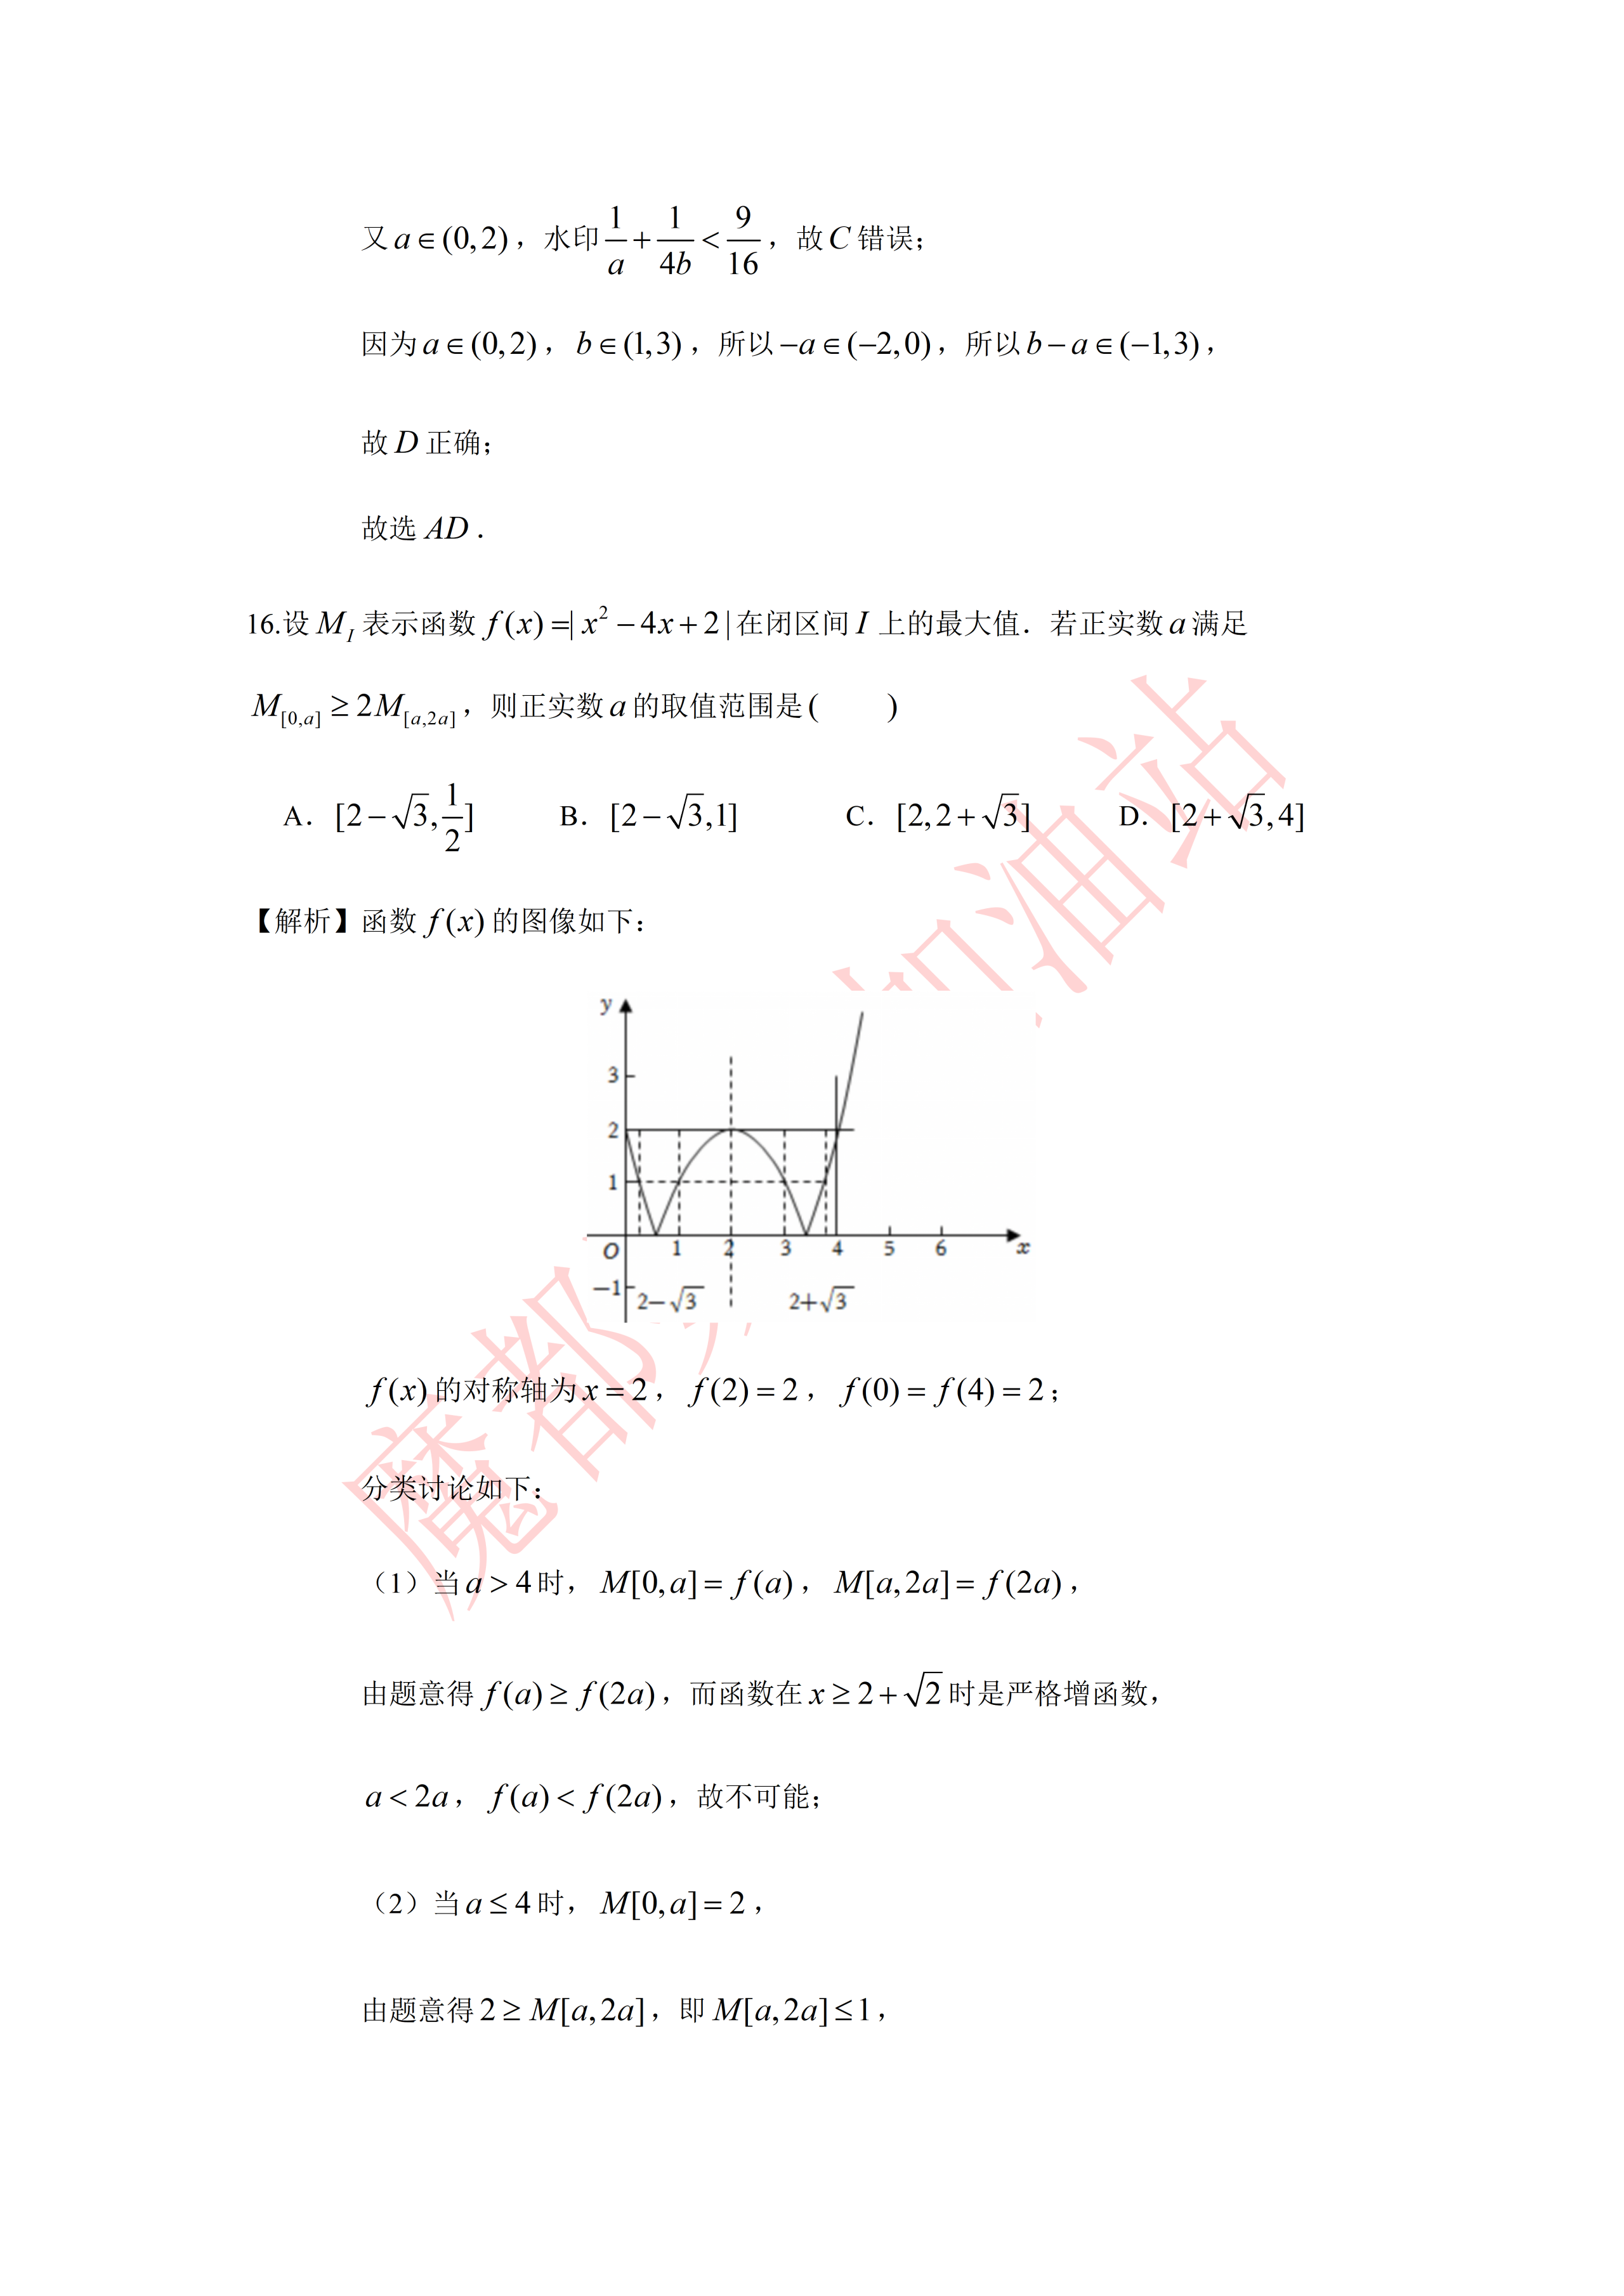
\includegraphics[width=.55\linewidth,trim=895bp 1535bp 915bp 1525bp,clip]{../原图/高一51_华师大二附中_国庆作业3/06.png}
\end{center}
\step{$f(x)$ 的对称轴为 $x=2$，$f(2)=2$，$f(0)=f(4)=2$；}
\step{分类讨论如下：}
\stepm{(1)}{当 $a>4$ 时，$M_{[0,a]}=f(a)$，$M_{[a,2a]}=f(2a)$，}
\step{由题意得 $f(a)\geqslant f(2a)$，而函数在 $x\geqslant2+\sqrt2$ 时是严格增函数，}
\step{$a<2a$，$f(a)<f(2a)$，故不可能；}
\stepm{(2)}{当 $a\leqslant4$ 时，$M_{[0,a]}=2$，}
\step{由题意得 $2\geqslant M_{[a,2a]}$，即 $M_{[a,2a]}\leqslant1$，}
\step{令 $f(x)=1$，解得 $x_1=2-\sqrt3$，$x_2=1$，$x_3=2+\sqrt3$，$x_4=3$，}
\step{则有 $a\geqslant2-\sqrt3$ 并且 $2a\leqslant1$，解得 $2-\sqrt3\leqslant a\leqslant\dfrac12$；}
\step{或者 $a\geqslant3$ 并且 $2a\leqslant2+\sqrt3$，无解；}
\step{故选 $A$.}
\solend

\fi

\end{enumerate}

\bigsec{三、解答题}

\begin{enumerate}
\setcounter{enumi}{16}

\item 已知 $M=\{x\mid2\leqslant x\leqslant5\}$，$N=\{x\mid a-1\leqslant x\leqslant2a+1\}$.
\begin{enumerate}[label=(\arabic*)]
\item 若 $M\subseteq N$，求实数 $a$ 的取值范围；
\item 若 $M\supseteq N$，求实数 $a$ 的取值范围.
\end{enumerate}

\ifanswer
\ans{（1）$[2,3]$；（2）$(-\infty,-2)$}
\fi

\ansspace[6]

\item 设集合 $A=\{x\mid|x+1|\leqslant3\}$，$B=\{x\mid0<x<3m\}$.
\begin{enumerate}[label=(\arabic*)]
\item 若 $A\cup B=A$，求实数 $m$ 的取值范围；
\item 设 $P=(\complement_R A)\cap B$，若 $\exists x\in\Z$ 且 $x\in P$，求实数 $m$ 的取值范围.
\end{enumerate}

\ifanswer
\solbegin
\stepm{(1)}{$A=\{x\mid|x+1|\leqslant3\}=\{x\mid-4\leqslant x\leqslant2\}$，且 $A\cup B=A$，所以 $B\subseteq A$.}
\step{若 $B=\varnothing$，此时 $0\geqslant3m$，解得 $m\leqslant0$；}
\step{若 $B\neq\varnothing$，此时 $0<3m$，且 $3m\leqslant2$，解得 $0<m\leqslant\dfrac23$；}
\step{则实数 $m$ 的取值范围是 $\left(-\infty,\dfrac23\right]$.}
\stepm{(2)}{因为 $\exists x\in\Z$ 且 $x\in P$，所以集合 $P$ 中至少存在一个整数.}
\step{$\complement_R A=\{x\mid x<-4\text{ 或 }x>2\}$，$B=\{x\mid0<x<3m\}$，}
\step{要使 $P=(\complement_R A)\cap B$ 中至少存在一个整数，则 $\begin{cases}3m>0\\3m>3\end{cases}$，解得 $m>1$，}
\step{则实数 $m$ 的取值范围是 $(1,+\infty)$.}
\solend

\fi

\ansspace[7]

\item 已知函数 $f(x)=x^2+(1-a)x-a(a\in\R)$.
\begin{enumerate}[label=(\arabic*)]
\item 解关于 $x$ 的不等式 $f(x)<0$；
\item 若 $\forall a\in[-1,1]$，$f(x)\geqslant0$ 恒成立，求实数 $x$ 的取值范围.
\end{enumerate}

\ifanswer
\solbegin
\stepm{(1)}{不等式 $x^2+(1-a)x-a<0$ 等价于 $(x-a)(x+1)<0$，}
\step{当 $a<-1$ 时，不等式的解集为 $(a,-1)$；}
\step{当 $a=-1$ 时，不等式的解集为 $\varnothing$；}
\step{当 $a>-1$ 时，不等式的解集为 $(-1,a)$.}
\stepm{(2)}{$x^2+(1-a)x-a=-a(x+1)+x^2+x$，}
\step{设 $g(a)=-a(x+1)+x^2+x$，$a\in[-1,1]$，}
\step{要使 $g(a)\geqslant0$ 在 $a\in[-1,1]$ 上恒成立，}
\step{只需 $\begin{cases}g(-1)\geqslant0\\g(1)\geqslant0\end{cases}$，即 $\begin{cases}x^2+2x+1\geqslant0\\x^2-1\geqslant0\end{cases}$，解得 $x\geqslant1$ 或 $x\leqslant-1$，}
\step{所以 $x$ 的取值范围为 $\{x\mid x\leqslant-1\text{ 或 }x\geqslant1\}$.}
\solend

\fi

\ansspace[7]

\item 若实数 $x$、$y$、$m$ 满足 $|x-m|>|y-m|$，则称 $x$ 比 $y$ 远离 $m$.
\begin{enumerate}[label=(\arabic*)]
\item 若 $2$ 比 $3x-4$ 远离 $1$，求 $x$ 的取值范围；
\item 设 $y=\dfrac{x+2}{x+1}$，其中 $x\in(0,\sqrt2)\cup(\sqrt2,+\infty)$，判断：$x$ 与 $y$ 哪一个更远离 $\sqrt2$？并说明理由.
\item 若 $x+y=2$，试问：$y$ 与 $x^2+y^2$ 哪一个更远离 $\dfrac12$？并说明理由.
\end{enumerate}

\ifanswer
\solbegin
\stepm{(1)}{由题意得 $|2-1|>|3x-4-1|$，所以 $|3x-5|<1$，解得 $\dfrac43<x<2$，}
\step{故 $x$ 的取值范围为 $\left(\dfrac43,2\right)$；}
\stepm{(2)}{$x$ 比 $y$ 更远离 $\sqrt2$，}
\step{理由如下：要证 $x$ 比 $y$ 更远离 $\sqrt2$，只要证 $|x-\sqrt2|>\left|\dfrac{x+2}{x+1}-\sqrt2\right|$，}
\step{即证 $|x-\sqrt2|>\left|\dfrac{(1-\sqrt2)(x-\sqrt2)}{x+1}\right|$，}
\step{因为 $x\in(0,\sqrt2)\cup(\sqrt2,+\infty)$，所以 $|x-\sqrt2|>0$，}
\step{所以只要证 $1>\dfrac{\sqrt2-1}{|x+1|}$，即证 $|x+1|>\sqrt2-1$，}
\step{因为 $x\in(0,\sqrt2)\cup(\sqrt2,+\infty)$，所以 $x+1\in(1,\sqrt2+1)\cup(\sqrt2+1,+\infty)$，}
\step{所以 $|x+1|>1>\sqrt2-1$，所以 $x$ 比 $y$ 更远离 $\sqrt2$；}
\stepm{(3)}{因为 $x^2+y^2\geqslant\dfrac{(x+y)^2}{2}=2$，当且仅当 $x=y=1$ 时等号成立，}
\step{所以 $\left|x^2+y^2-\dfrac12\right|=x^2+y^2-\dfrac12$，}
\step{从而 $\left|y-\dfrac12\right|-\left|x^2+y^2-\dfrac12\right|=\left|y-\dfrac12\right|-\left(x^2+y^2-\dfrac12\right)$，}
\step{①$y\geqslant\dfrac12$，$\left|y-\dfrac12\right|-\left|x^2+y^2-\dfrac12\right|=y-\dfrac12-\left(x^2+y^2-\dfrac12\right)=y-x^2-y^2$}
\step{$=y-(2-y)^2-y^2=-2y^2+5y-4=-2\left(y-\dfrac54\right)^2-\dfrac78<0$，}
\step{即 $\left|y-\dfrac12\right|<\left|x^2+y^2-\dfrac12\right|$；}
\step{②$y<\dfrac12$，}
\step{$\left|y-\dfrac12\right|-\left|x^2+y^2-\dfrac12\right|=\left(\dfrac12-y\right)-\left(x^2+y^2-\dfrac12\right)=-y-x^2-y^2+1$}
\step{$=-y-(2-y)^2-y^2+1=-2y^2+3y-3=-2\left(y-\dfrac34\right)^2-\dfrac{15}8<0$，}
\step{即 $\left|y-\dfrac12\right|<\left|x^2+y^2-\dfrac12\right|$；}
\step{综上，$\left|y-\dfrac12\right|<\left|x^2+y^2-\dfrac12\right|$，即 $x^2+y^2$ 比 $y$ 更远离 $\dfrac12$.}
\solend

\fi

\ansspace[9]

\item 对于非空有限整数集 $X$，$m\in\N^*$，定义 $X^m=\{x^m\mid x\in X\}$，对 $n\in\Z$，
$Y\oplus n=\{x+n\mid x\in Y\}$ 现有两个非空有限整数集 $A$、$B$，已知 $A\oplus1\subseteq B$ 且
$B^2\oplus(-4)\subseteq A$.
\begin{enumerate}[label=(\arabic*)]
\item 当 $A=\{-3,0\}$ 时求集合 $B$；
\item 证明：$A\subseteq\{-3,-2,0,1\}$；
\item 当 $A\oplus1=B$ 且 $B^2\oplus(-4)=A$ 时，任取 $a\in A$，$b\in B$ 构造函数
$f(x)=(x-a)(x-b)$ 问：当 $a$、$b$ 取何值时，$f(x)$ 的最小值最小？
\end{enumerate}

\ifanswer
\solbegin
\stepm{(1)}{因为 $A=\{-3,0\}$，$B^2\oplus(-4)\subseteq A$，}
\step{所以 $B^2\oplus(-4)$ 可能为 $\varnothing$、$\{-3\}$、$\{0\}$、$\{-3,0\}$，}
\step{当 $B^2\oplus(-4)=\varnothing$ 时 $B^2=\varnothing$，不满足非空，不合题意；}
\step{当 $B^2\oplus(-4)=\{-3\}$ 时 $B^2=\{1\}$，所以 $B=\{1,-1\}$、$\{1\}$、$\{-1\}$，}
\step{当 $B^2\oplus(-4)=\{0\}$ 时 $B^2=\{4\}$，所以 $B=\{2,-2\}$、$\{2\}$、$\{-2\}$，}
% 原卷如此，照录未改（此处作 $\{0,-3\}$，上一行同一集合作 $\{-3,0\}$）
\step{当 $B^2\oplus(-4)=\{0,-3\}$ 时 $B^2=\{4,1\}$，}
\step{所以 $B=\{1,2,-1,-2\}$、$\{2,-1,-2\}$、$\{2,1,-2\}$、$\{1,-1,-2\}$、$\{1,-1,2\}$、$\{1,2\}$、$\{-1,2\}$、$\{-1,-2\}$、$\{1,-2\}$，}
\step{又 $A\oplus1=\{-2,1\}\subseteq B$，得 $B$ 为 $\{1,-2\}$、$\{2,1,-2\}$、$\{1,-1,-2\}$、$\{1,2,-1,-2\}$.}
\stepm{(2)}{设 $x\in A$，因为 $A\oplus1\subseteq B$，所以 $x+1\in B$，}
\step{又 $B^2\oplus(-4)\subseteq A$，所以 $(x+1)^2-4\in A$，}
% 原卷如此，照录未改（此处及下文取 $x=2$ 处原卷均作 $(-4+1)^2-4=52-2a>0$）
\step{取 $x=-4$，则 $(-4+1)^2-4=52-2a>0$，$(5+1)^2-4=32\in A$，$\cdots$，}
\step{无限迭代，而 $A$ 为有限集，不合题意，舍去，即 $-4\notin A$；}
\step{取 $x=-3$，则 $(-3+1)^2-4=0\in A$，$(0+1)^2-4=-3\in A$，}
\step{得 $A$ 集合可为 $\{-3,0\}$；}
\step{取 $x=-2$，则 $(-2+1)^2-4=-3\in A$，$(-3+1)^2-4=0\in A$，}
\step{$(0+1)^2-4=-3\in A$，得 $A$ 集合可为 $\{-3,-2,0\}$；}
\step{取 $x=-1$，则 $(-1+1)^2-4=-4\in A$，又 $-4\notin A$，所以 $-1\notin A$，}
\step{取 $x=1$，则 $(1+1)^2-4=0\in A$，$(0+1)^2-4=-3\in A$，}
\step{$(-3+1)^2-4=0\in A$，得 $A$ 集合可为 $\{-3,0,1\}$，}
\step{取 $x=2$，则 $(2+1)^2-4=52-2a>0$，$(5+1)^2-4=32\in A$，$\cdots$，}
\step{无限迭代，而 $A$ 为有限集，不合题意，舍去，即 $2\notin A$，}
\step{同理当 $x<-4$ 或 $x>2$，且 $x\in\Z$ 时不符合 $A$ 为有限集，舍去；}
\step{故由上得 $A$ 集合可为 $\{-3,0\},\{-3,-2,0\},\{-3,0,1\},\{-3,-2,0,1\}$，}
\step{所以 $A\subseteq\{-3,-2,0,1\}$，}
\stepm{(3)}{当 $A\oplus1=B$ 且 $B^2\oplus(-4)=A$ 时，}
\step{设 $x\in B$，则 $x^2-4\in B^2\oplus(-4)=A$，}
% 原卷如此，照录未改（题设 $A=\{-3,0\}$，此处两个判别式取的是 $-2$ 与 $1$，均不属于 $A$）
\step{$x^2-4=-2$ 时 $x=\pm\sqrt2$，不为整数，不合题意；}
\step{$x^2-4=1$ 时 $x=\pm\sqrt5$，不为整数，不合题意；}
\step{所以 $A=\{-3,0\}$，又 $A\oplus1=B$，则 $B=\{-2,1\}$，}
\step{任取 $a\in A$，$b\in B$ 构造函数 $f(x)=(x-a)(x-b)$，}
\step{$f(x)=(x-a)(x-b)=x^2-(a+b)x+ab$}
\step{$=x^2-(a+b)x+\dfrac{(a+b)^2}{4}+ab-\dfrac{(a+b)^2}{4}$}
\step{$=\left[x-\dfrac{(a+b)}2\right]^2-\dfrac{(a-b)^2}{4}\geqslant-\dfrac{(a-b)^2}{4}$，所以 $f(x)_{min}=-\dfrac{(a-b)^2}{4}$，}
\step{又 $a\in A=\{-3,0\}$，$b\in B=\{-2,1\}$，所以 $a-b$ 的取值有 $-1,-4,2$，}
\step{所以 $f(x)_{min}=-\dfrac{(a-b)^2}{4}\geqslant-\dfrac{(-3-1)^2}{4}=-4$，}
\step{即当 $a=-3$，$b=1$ 时 $f(x)_{min}$ 的最小值为 $-4$.}
\solend

\fi

\ansspace*[12]

\end{enumerate}

\end{document}
"
% 紧凑版：xelatex "\def\iscompact{1}% 高一51_华师大二附中_国庆作业3.tex
%   —— 高一上数学“2026-2027 年华师大二附中高一上国庆作业 3”（讲评版）
% 试卷版：xelatex 高一51_华师大二附中_国庆作业3.tex
% 答案版：xelatex "\def\isanswer{1}\input{高一51_华师大二附中_国庆作业3.tex}"
% 紧凑版：xelatex "\def\iscompact{1}\input{高一51_华师大二附中_国庆作业3.tex}"
%
% 原始材料：微信公众号“魔都数学加油站”文章，作者破晓，连载“27学年高一51”；
% 原文标题“27学年高一51——2026-2027年上海市华师大二附中高一上国庆作业3”；
% 原文链接：https://mp.weixin.qq.com/s/95SLMEmPUT30s4U7wjr5Og。
% 该页面用 JS 渲染，未见明确发布日期；页面内时间戳约为 2026-10-05 21:37，本稿以该时刻记可得日期。
% 正文为 12 张 PNG 页：第 01、02、03、05、07、08、11 页 4762×6735，
% 第 04、06、09、10、12 页 2560×3620。按页序逐页读取，12 页全为试卷正文页
% （卷首标题在第 1 页页顶，卷末解答题止于第 12 页），无封面页、目录页或单独的页脚页。
% 卷面标题照原卷印作“2026-2027 年华师大二附中高一上国庆作业 3”（公众号标题中的“上海市”
% 卷面标题行没有，本稿照卷面），年份区间按全稿惯例排 en dash。
%
% 篇幅与题号：原卷自第 3 题起编号（第 1、2 题不在本卷内）。填空题 3—12（10 题）、
% 选择题 13—16（4 题）、解答题 17—21（5 题），共 19 题。本稿沿用原节与原题号，
% 只改排为全稿统一的大节样式（原卷小节标题为“一、填空题”“二、选择题”“三、解答题”）。
% 正文为讲评版：填空题 3—12 与选择题 13—16 只印【解析】（选择题的结论“故选 X”印在解析内），
% 按全稿口径这类题不另提 \ans{}；解答题第 17 题只印【答案】，故只给 \ans{}；
% 第 18—21 题只印【解析】。
%
% 副标题：原卷未印副标题。本稿按“知识模块”口径标作“集合与常用逻辑用语、不等式”：
% 19 题中集合与常用逻辑用语 8 题（3、4、6、10、13、17、18、21），
% 不等式（含函数最值、绝对值不等式）11 题（5、7、8、9、11、12、14、15、16、19、20），
% 两类均远超三分之一，故并标。口径同 高一46_交附闵行_国庆作业3、高一48_华师大二附中_周末作业2。
%
% 与原卷的排版差异：
%   ① 原卷每题下直接印【答案】或【解析】，本稿按全稿惯例将答案与解析置于答案版；
%   ② 原卷未印副标题，本稿按“知识模块”口径补出；
%   ③ 原卷填空横线按全稿惯例排为 \blankline[4.4em]；
%   ④ 原卷 $R$、$N$、$Z$ 均排斜体，本稿按全稿惯例改用花体 $\R$、$\N$、$\Z$（同 高一48）；
%   ⑤ 原卷第 12 题解析配图、第 13 题题干韦恩图都印在正文右侧的浮动位置，第 16 题解析配图
%      印在解析行间；本稿三图一律居中排，均自原图对应页裁切（trim），不另存图片文件；
%   ⑥ 原卷解答题未留作答空白，本稿按全稿惯例加 \ansspace；
%   ⑦ 原卷第 15 题解析第 7、8 两个印刷行是一串连等式的折行，本稿按“一条 \step ＝ 一个印刷行”
%      的口径分成两条 \step。
%
% 原卷笔误/存疑（均照录未改，正文对应处另有 % 注）：
%   ① 第 12 题解析末行作“区间长度之和为 $x_1-b+x_2-a=x_1-x_2-a-b=2+a+b-a-b=2$”，
%      按上一行 $x_1+x_2=2+a+b$，此处应为 $x_1+x_2$；原卷作 $x_1-x_2$。
%   ② 第 15 题解析“又 $a\in(0,2)$，”与 $\dfrac1a+\dfrac1{4b}<\dfrac9{16}$ 之间，
%      原卷正文夹印“水印”二字（系制版遗留字样，非试卷内容）。
%   ③ 第 21 题第 (2) 问解析两处（取 $x=-4$、取 $x=2$）作“$=52-2a>0$”，
%      与题设 $(x+1)^2-4$ 的取值（按 $x=-4$ 应为 $5$）不符，当系原卷算式遗留。
%   ④ 第 21 题第 (1) 问解析先写 $B^2\oplus(-4)$ 可能为 $\{-3,0\}$，后文又作 $\{0,-3\}$，
%      同一集合两种写法。
%   ⑤ 第 21 题第 (3) 问解析：题设 $B^2\oplus(-4)=A$ 且 $A=\{-3,0\}$ 时，由 $x^2-4\in A$
%      应得 $x^2-4=-3$ 或 $0$；原卷讨论的却是 $x^2-4=-2$ 与 $x^2-4=1$（两值均不属于 $A$），
%      与题设不合。
%
% 插图：3 张，均自原图裁切（无 \begin{tikzpicture} 重排）：
%   · 第 13 题题干韦恩图（原图第 04 页，图在题干与选项右侧）
%   · 第 12 题解析配图（原图第 04 页，图在解析右侧）
%   · 第 16 题解析配图（原图第 06 页，图在解析中间）
%
\documentclass[a4paper,11pt]{article}
\usepackage{common}

\begin{document}

\examtitlest[3]{2026--2027 年华师大二附中高一上国庆作业 3}{集合与常用逻辑用语、不等式}

\bigsec{一、填空题}

\begin{enumerate}
\setcounter{enumi}{2}

\item 若 $\{x\mid x<1\text{ 或 }x>4\}\cup\{x\mid m<x<2m+3\}=R$，则实数 $m$ 的取值范围为\blankline[4.4em].

\ifanswer
\solbegin
\step{因为 $\{x\mid x<1\text{ 或 }x>4\}\cup\{x\mid m<x<2m+3\}=R$，}
\step{所以 $\begin{cases}m<1\\2m+3>4\end{cases}$，解得 $\dfrac12<m<1$，所以 $m$ 的取值范围为 $\left(\dfrac12,1\right)$.}
\solend

\fi

\item 若“$x\leqslant5$”是“$x<a$”的必要不充分条件，则 $a$ 的取值范围是\blankline[4.4em].

\ifanswer
\solbegin
\step{若“$x\leqslant5$”是“$x<a$”的必要不充分条件，则 $\{x\mid x<a\}\subset\{x\mid x\leqslant5\}$，}
\step{所以 $a\leqslant5$.}
\solend

\fi

\item 实数 $x$、$y$ 满足 $x^2+2xy+4y^2=1$，则 $x+2y$ 的取值范围是\blankline[4.4em].

\ifanswer
\solbegin
\step{因为 $x^2+2xy+4y^2=(x+2y)^2-2xy=1$，}
\step{所以 $(x+2y)^2-1=x\cdot(2y)\leqslant\left(\dfrac{x+2y}{2}\right)^2$，当且仅当 $x=2y$ 时取等号，}
\step{解得 $-\dfrac{2\sqrt3}{3}\leqslant x+2y\leqslant\dfrac{2\sqrt3}{3}$，故 $x+2y$ 的取值范围是 $\left[-\dfrac{2\sqrt3}{3},\dfrac{2\sqrt3}{3}\right]$.}
\solend

\fi

\item 若命题 $p$：“$\exists x\in\R$，$5x^2-3x+m=0$”为假命题，则实数 $m$ 的取值范围为\blankline[4.4em].

\ifanswer
\solbegin
\step{若命题 $p$：$\exists x\in\R$，$5x^2-3x+m=0$ 为假命题，}
\step{则 $5x^2-3x+m=0$ 没有实数根，故 $\Delta=9-20m<0$，解得 $m>\dfrac9{20}$.}
\solend

\fi

\item 若当 $3\leqslant m\leqslant5$ 时，$mx^2-mx+m-9<0$ 有解，则实数 $x$ 的取值范围是\blankline[4.4em].

\ifanswer
\solbegin
\step{当 $3\leqslant m\leqslant5$ 时，$mx^2-mx+m-9<0$ 有解，}
\step{即 $(x^2-x+1)m-9<0$ 在 $m\in[3,5]$ 上有解，}
\step{因为 $x^2-x+1>0$，所以一次函数 $g(m)=(x^2-x+1)m-9$ 严格增，}
\step{所以只需 $g(3)=3x^2-3x-6<0$ 即可，}
\step{即 $x^2-x-2<0$，$(x-2)(x+1)<0$，解得 $-1<x<2$，}
\step{所以实数 $x$ 的取值范围是 $(-1,2)$.}
\solend

\fi

\item 已知不等式 $\dfrac{x}{x^2+4}\leqslant a$ 对任意的 $x\in[1,3]$ 恒成立，则实数 $a$ 的范围为\blankline[4.4em].

\ifanswer
\solbegin
\step{因为 $x\in[1,3]$，所以 $\dfrac{x}{x^2+4}=\dfrac{1}{x+\dfrac4x}\leqslant\dfrac{1}{2\sqrt{x\times\dfrac4x}}=\dfrac14$，}
\step{当且仅当 $x=\dfrac4x$ 时，即 $x=2$ 时取等号，即 $\dfrac{x}{x^2+4}$ 在 $x\in[1,3]$ 的最大值为 $\dfrac14$，}
\step{又由不等式 $\dfrac{x}{x^2+4}\leqslant a$ 对任意的 $x\in[1,3]$ 恒成立，所以 $a\geqslant\dfrac14$，}
\step{即实数 $a$ 的范围为 $\left[\dfrac14,+\infty\right)$.}
\solend

\fi

\item 甲、乙两人解关于 $x$ 的不等式 $x^2+bx+c<0$，甲写错了 $b$，正确计算后得到的解为 $\{x\mid1<x<2\}$；
乙写错了 $c$，正确计算后得到的解为 $\{x\mid-4<x<1\}$. 那么不等式 $\dfrac{bx+c}{x-2}<0$ 的解为\blankline[4.4em].

\ifanswer
\solbegin
\step{由 $x^2+bx+c<0$ 的解为 $\{x\mid1<x<2\}$，}
\step{则 $1$ 和 $2$ 是方程 $x^2+bx+c=0$ 的两个根，}
\step{甲写错了 $b$，但 $c$ 是正确的，所以 $c=1\times2=2$；}
\step{由 $x^2+bx+c<0$ 的解为 $\{x\mid-4<x<1\}$，}
\step{则 $-4$ 和 $1$ 是方程 $x^2+bx+c=0$ 的两个根，}
\step{乙写错了 $c$，但 $b$ 是正确的，所以 $-b=-4+1=-3$，即 $b=3$.}
\step{由 $\dfrac{bx+c}{x-2}<0$，得 $\dfrac{3x+2}{x-2}<0$，即 $(3x+2)(x-2)<0$，解得 $-\dfrac23<x<2$.}
\step{不等式 $\dfrac{bx+c}{x-2}<0$ 的解为 $\left\{x\mid-\dfrac23<x<2\right\}$.}
\solend

\fi

\item 已知 $\dfrac{1}{x-2}\geqslant1$ 是 $|x-a|<2$ 的充分非必要条件，则实数 $a$ 的取值范围是\blankline[4.4em].

\ifanswer
\solbegin
\step{由 $\dfrac{1}{x-2}\geqslant1$ 得 $\dfrac{3-x}{x-2}\geqslant0$，解得 $2<x\leqslant3$，由 $|x-a|<2$ 得 $a-2<x<a+2$，}
\step{因为 $\dfrac{1}{x-2}\geqslant1$ 是 $|x-a|<2$ 的充分非必要条件，}
\step{所以 $\{x\mid2<x\leqslant3\}\subset\{x\mid a-2<x<a+2\}$，所以 $\begin{cases}a-2\leqslant2\\a+2>3\end{cases}$，解得 $1<a\leqslant4$，}
\step{即实数 $a$ 的取值范围是 $(1,4]$.}
\solend

\fi

\item 设 $a>0$，$b>0$，若不等式 $a(a+1)^2+b(b+1)^2\geqslant\lambda ab$ 恒成立，则实数 $\lambda$ 的最大值为\blankline[4.4em].

\ifanswer
\solbegin
\step{$a(a+1)^2+b(b+1)^2\geqslant\lambda ab\Leftrightarrow\lambda\leqslant\dfrac{a(a+1)^2+b(b+1)^2}{ab}=\dfrac{(a+1)^2}{b}+\dfrac{(b+1)^2}{a}$，}
\step{从而原问题转化为求 $\dfrac{(a+1)^2}{b}+\dfrac{(b+1)^2}{a}$ 的最小值.}
\step{因为 $\dfrac{(a+1)^2}{b}+\dfrac{(b+1)^2}{a}=\dfrac{b^2+2b+1}{a}+\dfrac{a^2+2a+1}{b}$}
\step{$=\left(\dfrac{b^2}{a}+\dfrac{a^2}{b}\right)+2\left(\dfrac ba+\dfrac ab\right)+\left(\dfrac1a+\dfrac1b\right)\geqslant2\sqrt{\dfrac{b^2}{a}\cdot\dfrac{a^2}{b}}+2\times2\sqrt{\dfrac ba\cdot\dfrac ab}+2\sqrt{\dfrac1a\cdot\dfrac1b}$}
\step{$=2\sqrt{ab}+4+\dfrac{2}{\sqrt{ab}}\geqslant2\sqrt{2\sqrt{ab}\cdot\dfrac{2}{\sqrt{ab}}}+4=8$，以上均当且仅当 $a=b$ 时取等号，}
\step{所以 $\lambda\leqslant8$，即实数 $\lambda$ 的最大值为 $8$.}
\solend

\fi

\item 定义区间 $(a,d)$、$[a,d)$、$(a,d]$、$[a,d]$ 的长度为 $d-a$（$d>a$），已知 $a>b$，则满足
$\dfrac{1}{x-a}+\dfrac{1}{x-b}\geqslant1$ 的 $x$ 构成的区间的长度之和为\blankline[4.4em].

\ifanswer
\solbegin
\step{因为 $\dfrac{1}{x-a}+\dfrac{1}{x-b}\geqslant1$，所以 $\dfrac{2x-(a+b)}{(x-a)(x-b)}\geqslant1$，}
\step{即 $\dfrac{2x-(a+b)}{(x-a)(x-b)}-1\geqslant0$，则 $\dfrac{x^2-(2+a+b)x+ab+a+b}{(x-a)(x-b)}\leqslant0$，}
\step{设 $x^2-(2+a+b)x+ab+a+b=0$ 的根为 $x_1$ 和 $x_2$，}
\begin{center}
% 原卷该图印在解析右侧（原图第 04 页），本稿移作居中排，直接裁取原图，不另存图片文件。
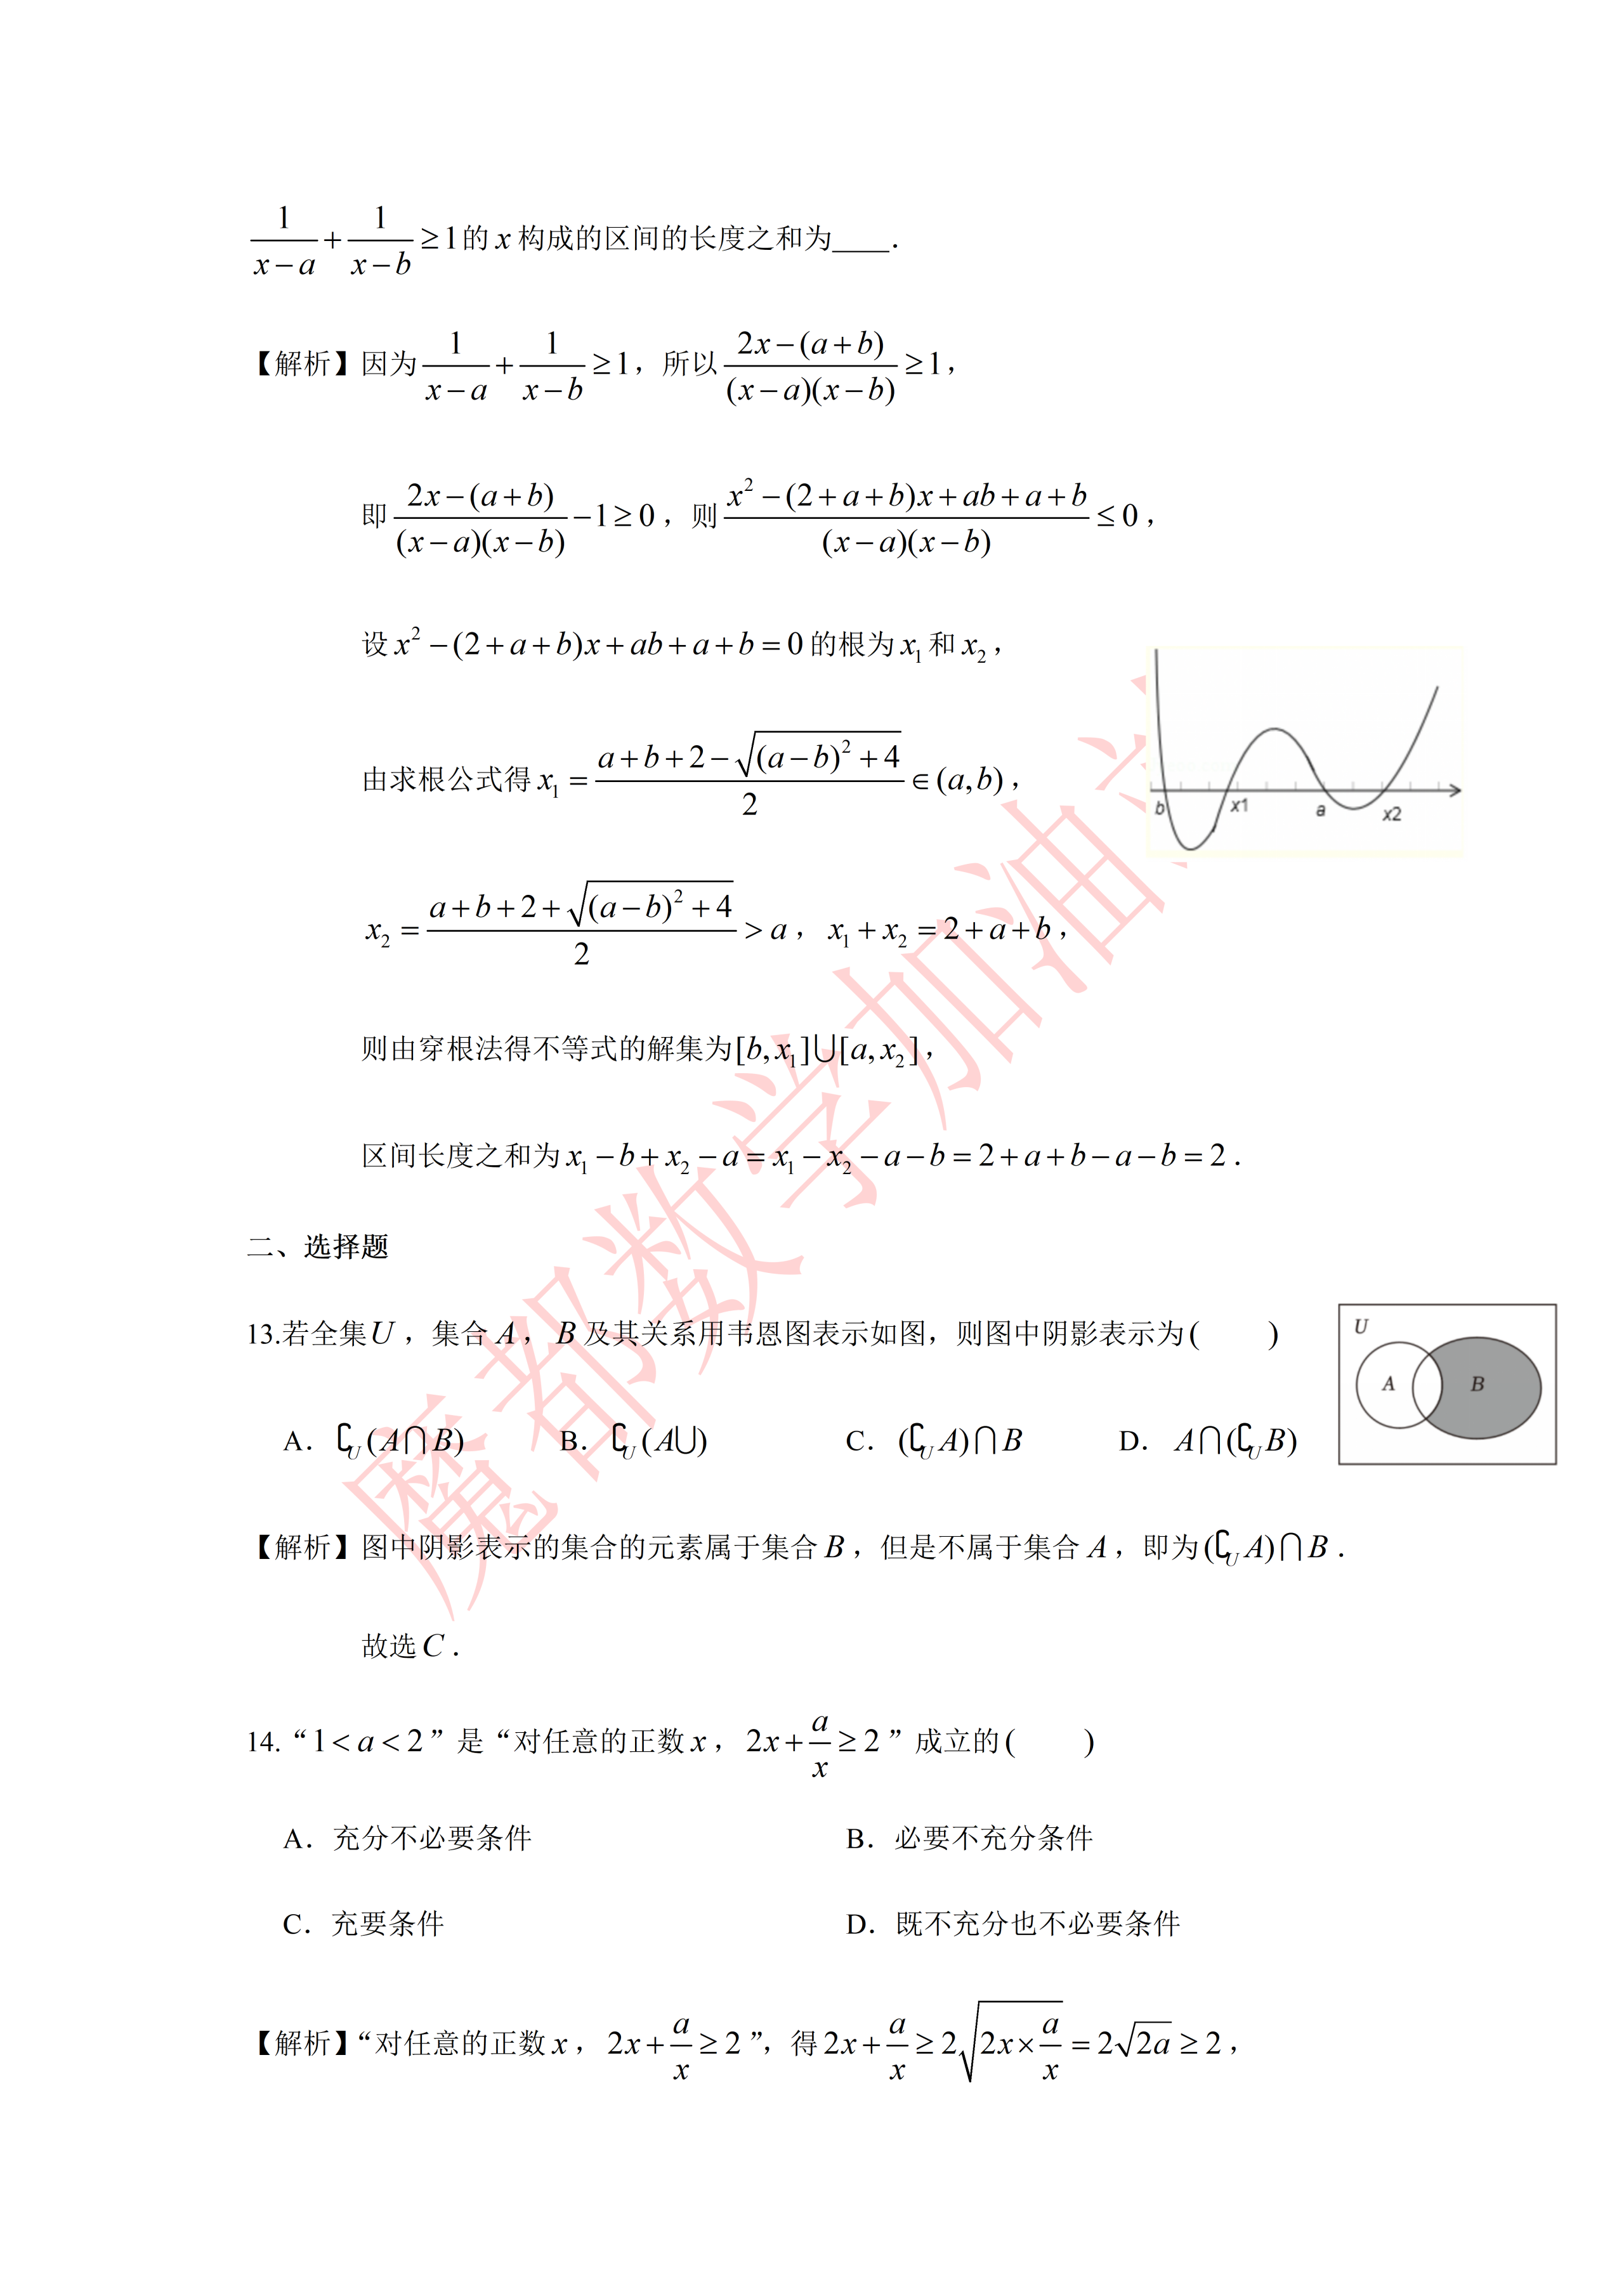
\includegraphics[width=.50\linewidth,trim=1786bp 2255bp 228bp 985bp,clip]{../原图/高一51_华师大二附中_国庆作业3/04.png}
\end{center}
\step{由求根公式得 $x_1=\dfrac{a+b+2-\sqrt{(a-b)^2+4}}{2}\in(a,b)$，}
\step{$x_2=\dfrac{a+b+2+\sqrt{(a-b)^2+4}}{2}>a$，$x_1+x_2=2+a+b$，}
\step{则由穿根法得不等式的解集为 $[b,x_1]\cup[a,x_2]$，}
% 原卷如此，照录未改（此处原卷作 $x_1-x_2$，按上一行 $x_1+x_2=2+a+b$ 当为 $x_1+x_2$）
\step{区间长度之和为 $x_1-b+x_2-a=x_1-x_2-a-b=2+a+b-a-b=2$.}
\solend

\fi

\end{enumerate}

\bigsec{二、选择题}

\begin{enumerate}
\setcounter{enumi}{12}

% 本题是“题干 + 图 + 选项”约 5.5cm 的一整块，图夹在题干与选项之间时 \keepwithprev 挡不住断点，
% 故按 高一30 第 13 题的成例在题前先量一次页高（守卫放在 \item 之前）。
\needvspace{6cm}
\item 若全集 $U$，集合 $A$、$B$ 及其关系用韦恩图表示如图，则图中阴影表示为\mbox{（\quad）}

\begin{center}
% 原卷该图印在题干与选项右侧（原图第 04 页），本稿移作居中排，直接裁取原图，不另存图片文件。
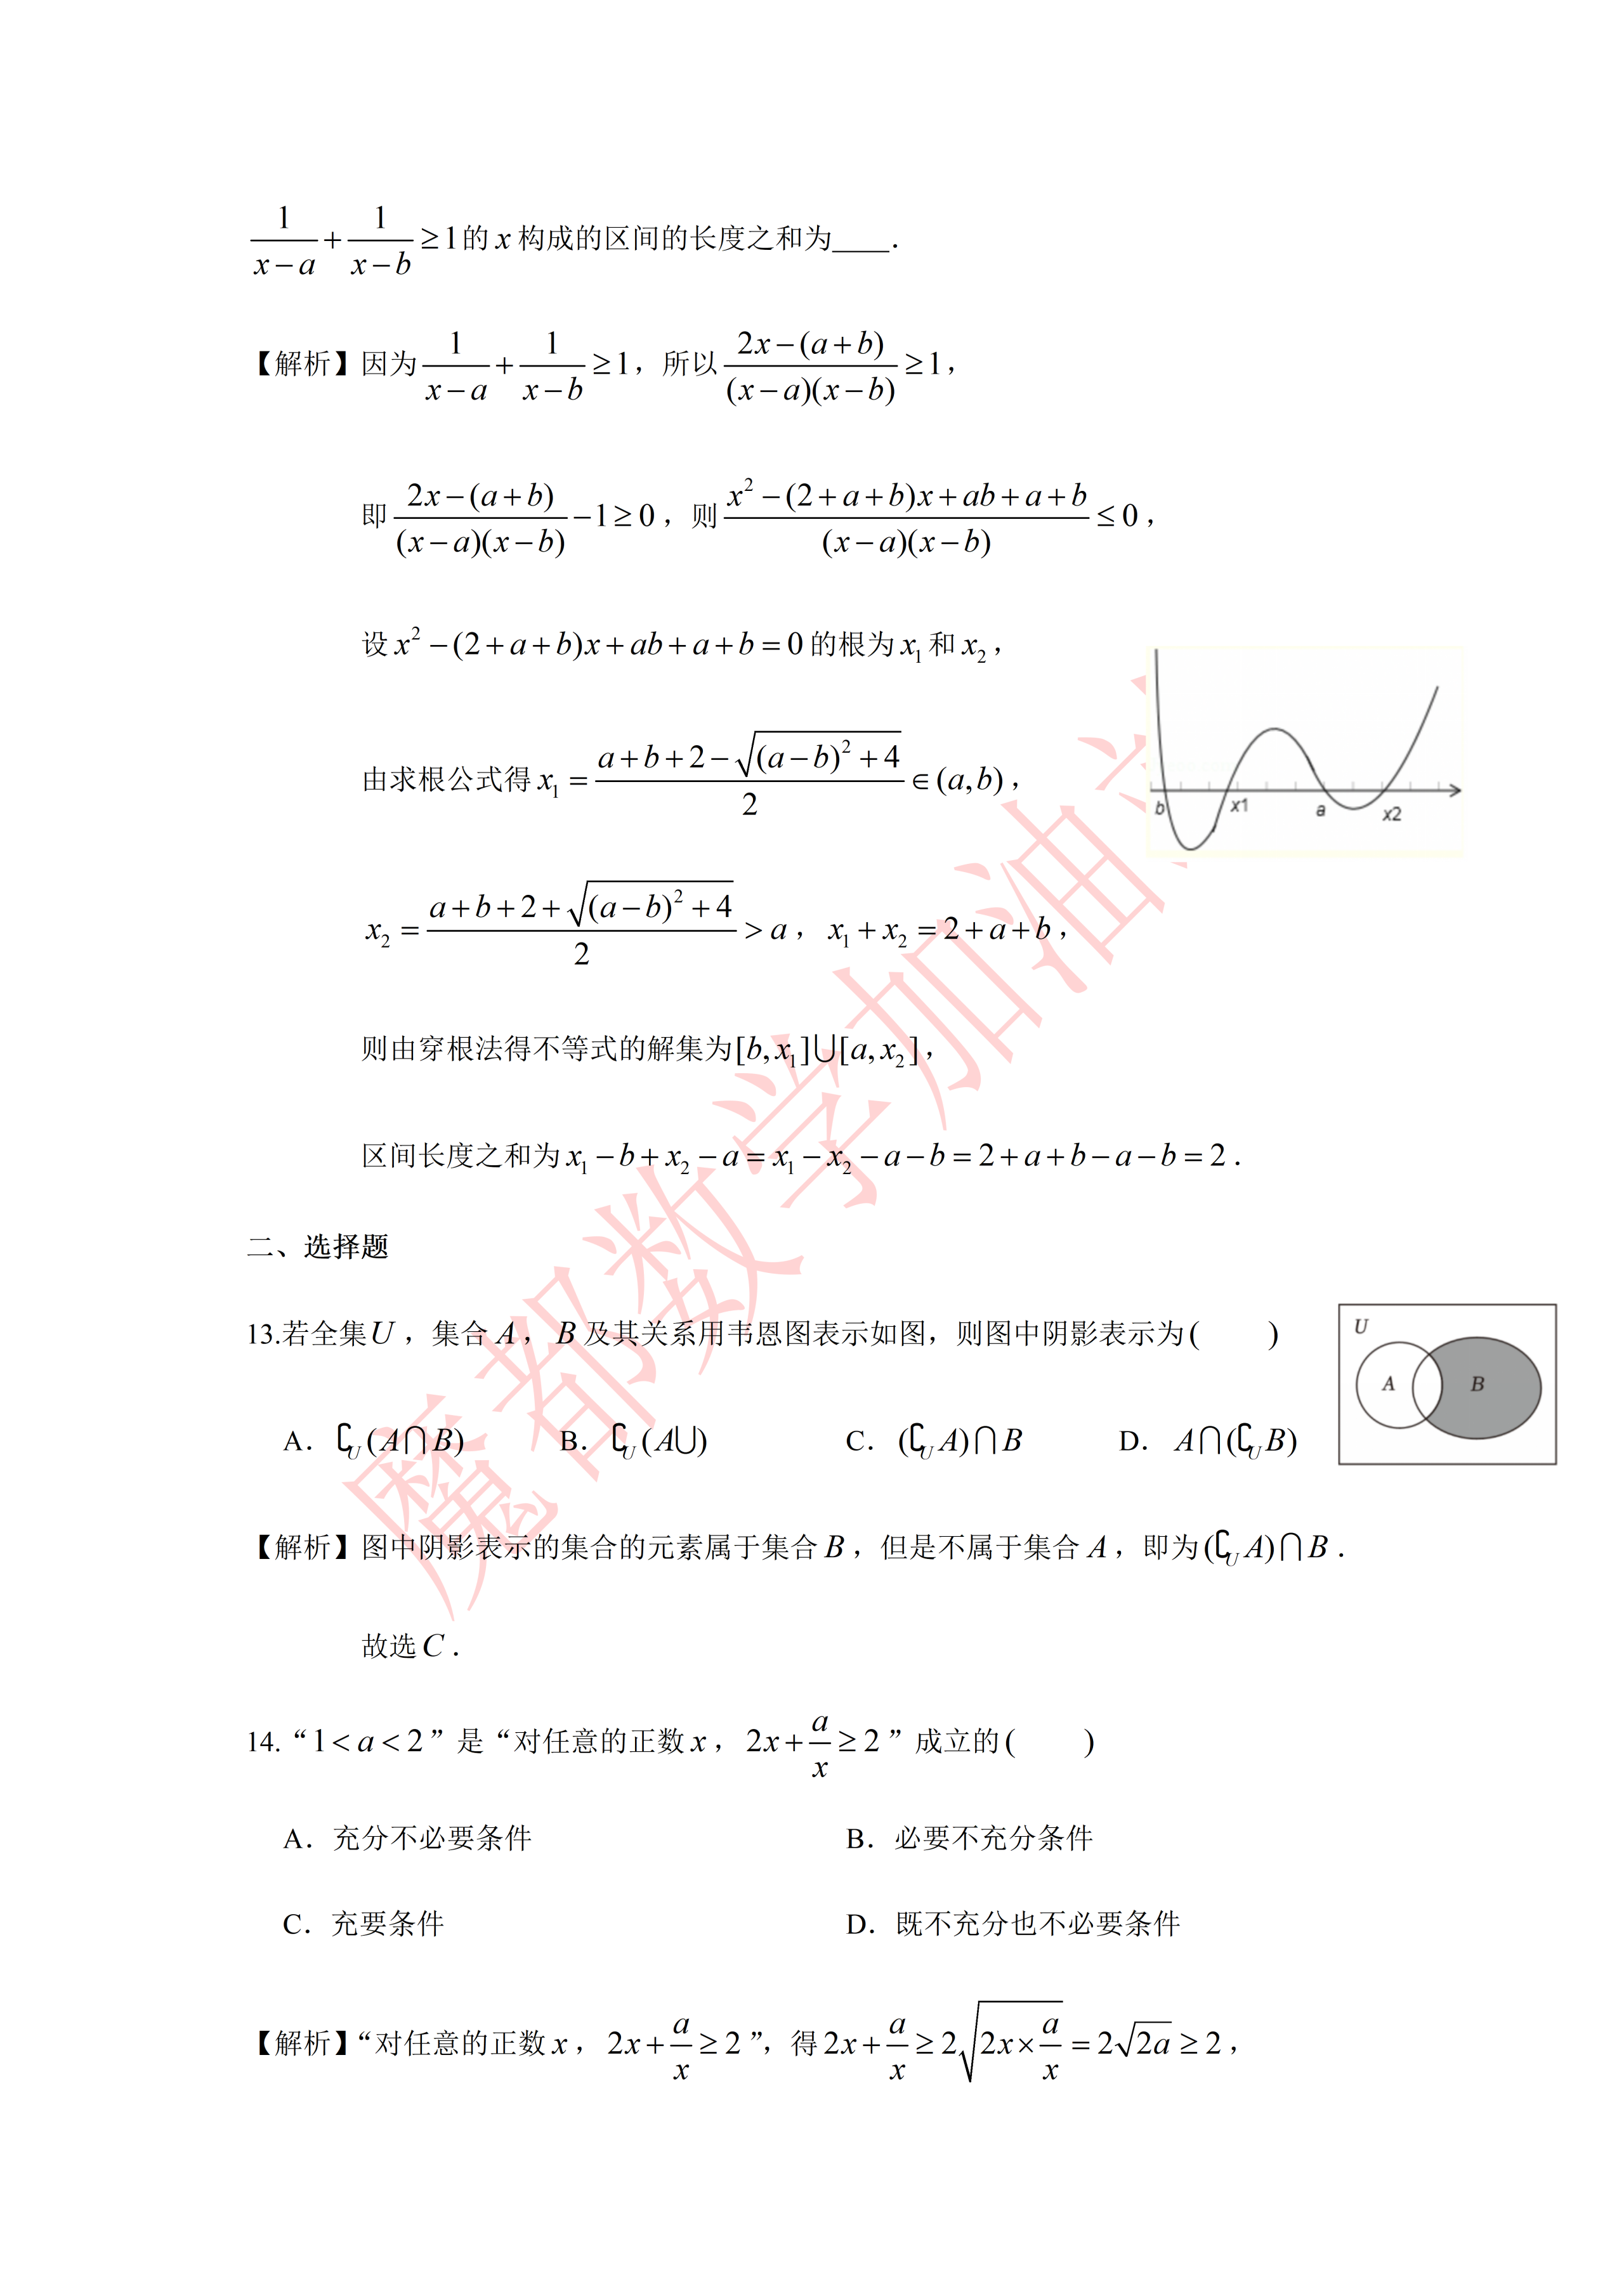
\includegraphics[width=.30\linewidth,trim=2105bp 1308bp 105bp 2050bp,clip]{../原图/高一51_华师大二附中_国庆作业3/04.png}
\end{center}

\keepwithprev
A. $\complement_U(A\cap B)$\qquad B. $\complement_U(A\cup B)$

C. $(\complement_U A)\cap B$\qquad D. $A\cap(\complement_U B)$

\ifanswer
\solbegin
\step{图中阴影表示的集合的元素属于集合 $B$，但是不属于集合 $A$，即为 $(\complement_U A)\cap B$.}
\step{故选 $C$.}
\solend

\fi

\item “$1<a<2$”是“对任意的正数 $x$，$2x+\dfrac ax\geqslant2$”成立的\mbox{（\quad）}

\keepwithprev
A. 充分不必要条件\qquad B. 必要不充分条件

C. 充要条件\qquad\qquad D. 既不充分也不必要条件

\ifanswer
\solbegin
\step{“对任意的正数 $x$，$2x+\dfrac ax\geqslant2$”，得 $2x+\dfrac ax\geqslant2\sqrt{2x\times\dfrac ax}=2\sqrt{2a}\geqslant2$，}
\step{所以 $\sqrt{2a}\geqslant1$，解得 $a\geqslant\dfrac12$，}
\step{若“$1<a<2$”得 $2x+\dfrac ax\geqslant2\sqrt{2x\times\dfrac ax}=2\sqrt{2a}>2\sqrt2>2$，}
\step{所以“$1<a<2$”$\Rightarrow$“对任意的正数 $x$，$2x+\dfrac ax\geqslant2$”，}
\step{所以“$1<a<2$”是“对任意的正数 $x$，$2x+\dfrac ax\geqslant2$”成立的充分不必要条件，}
\step{故选 $A$.}
\solend

\fi

\item 已知函数 $f(x)=2x-3$，$x\in(0,2)$，实数 $a$、$b$ 满足 $f(a)+f(b-1)=0$，则以下成立的有\mbox{（\quad）}

\keepwithprev
A. $a(b-1)$ 的最大值为 $\dfrac94$\qquad\qquad B. $b-\dfrac1a$ 的最大值为 $2$

C. $\dfrac1a+\dfrac1{4b}$ 的最小值为 $\dfrac9{16}$\qquad D. $-1<b-a<3$

\ifanswer
\solbegin
\step{因为函数 $f(x)=2x-3$，$x\in(0,2)$，实数 $a$、$b$ 满足 $f(a)+f(b-1)=0$，}
\step{所以 $2a-3+2(b-1)-3=0$，得 $a+b=4$，$a\in(0,2)$，$b\in(1,3)$，}
\step{所以 $a(b-1)=a(3-a)=-\left(a-\dfrac32\right)^2+\dfrac94$，$a\in(0,2)$，}
\step{所以 $0<a(b-1)\leqslant\dfrac94$，故选项 $A$ 正确；}
\step{$b-\dfrac1a=4-a-\dfrac1a=4-\left(a+\dfrac1a\right)\leqslant4-2=2$，}
\step{当且仅当 $a=1$，$b=3$ 时取等号，又 $b\in(1,3)$，故 $b-\dfrac1a<2$，故 $B$ 错误；}
\step{$\dfrac1a+\dfrac1{4b}=\dfrac14\left(\dfrac1a+\dfrac1{4b}\right)(a+b)=\dfrac14\left(1+\dfrac14+\dfrac ba+\dfrac a{4b}\right)=\dfrac5{16}+\dfrac14\left(\dfrac ba+\dfrac a{4b}\right)$}
\step{$\geqslant\dfrac5{16}+\dfrac14\cdot2\sqrt{\dfrac ba\cdot\dfrac a{4b}}=\dfrac9{16}$，当且仅当 $\dfrac ba=\dfrac a{4b}$，即 $a=2b=\dfrac83$ 时取等号，}
% 原卷如此，照录未改（“又 $a\in(0,2)$，”与下式之间原卷正文夹印“水印”二字）
\step{又 $a\in(0,2)$，水印 $\dfrac1a+\dfrac1{4b}<\dfrac9{16}$，故 $C$ 错误；}
\step{因为 $a\in(0,2)$，$b\in(1,3)$，所以 $-a\in(-2,0)$，所以 $b-a\in(-1,3)$，}
\step{故 $D$ 正确；}
\step{故选 $AD$.}
\solend

\fi

% 本题解析含图（“函数 f(x) 的图像如下”），图夹在解析行间，页末放不下会被拆开，
% 故在题前先量一次页高；上界取“题干 + 选项 + 图 + 首行解析”一块的高度。
\needvspace{6cm}
\item 设 $M_I$ 表示函数 $f(x)=|x^2-4x+2|$ 在闭区间 $I$ 上的最大值. 若正实数 $a$ 满足
$M_{[0,a]}\geqslant2M_{[a,2a]}$，则正实数 $a$ 的取值范围是\mbox{（\quad）}

\keepwithprev
A. $\left[2-\sqrt3,\dfrac12\right]$\qquad B. $[2-\sqrt3,1]$

C. $[2,2+\sqrt3]$\qquad\qquad D. $[2+\sqrt3,4]$

\ifanswer
\solbegin
\step{函数 $f(x)$ 的图像如下：}
\begin{center}
% 原卷该图印在解析行间（原图第 06 页），本稿直接裁取原图，不另存图片文件。
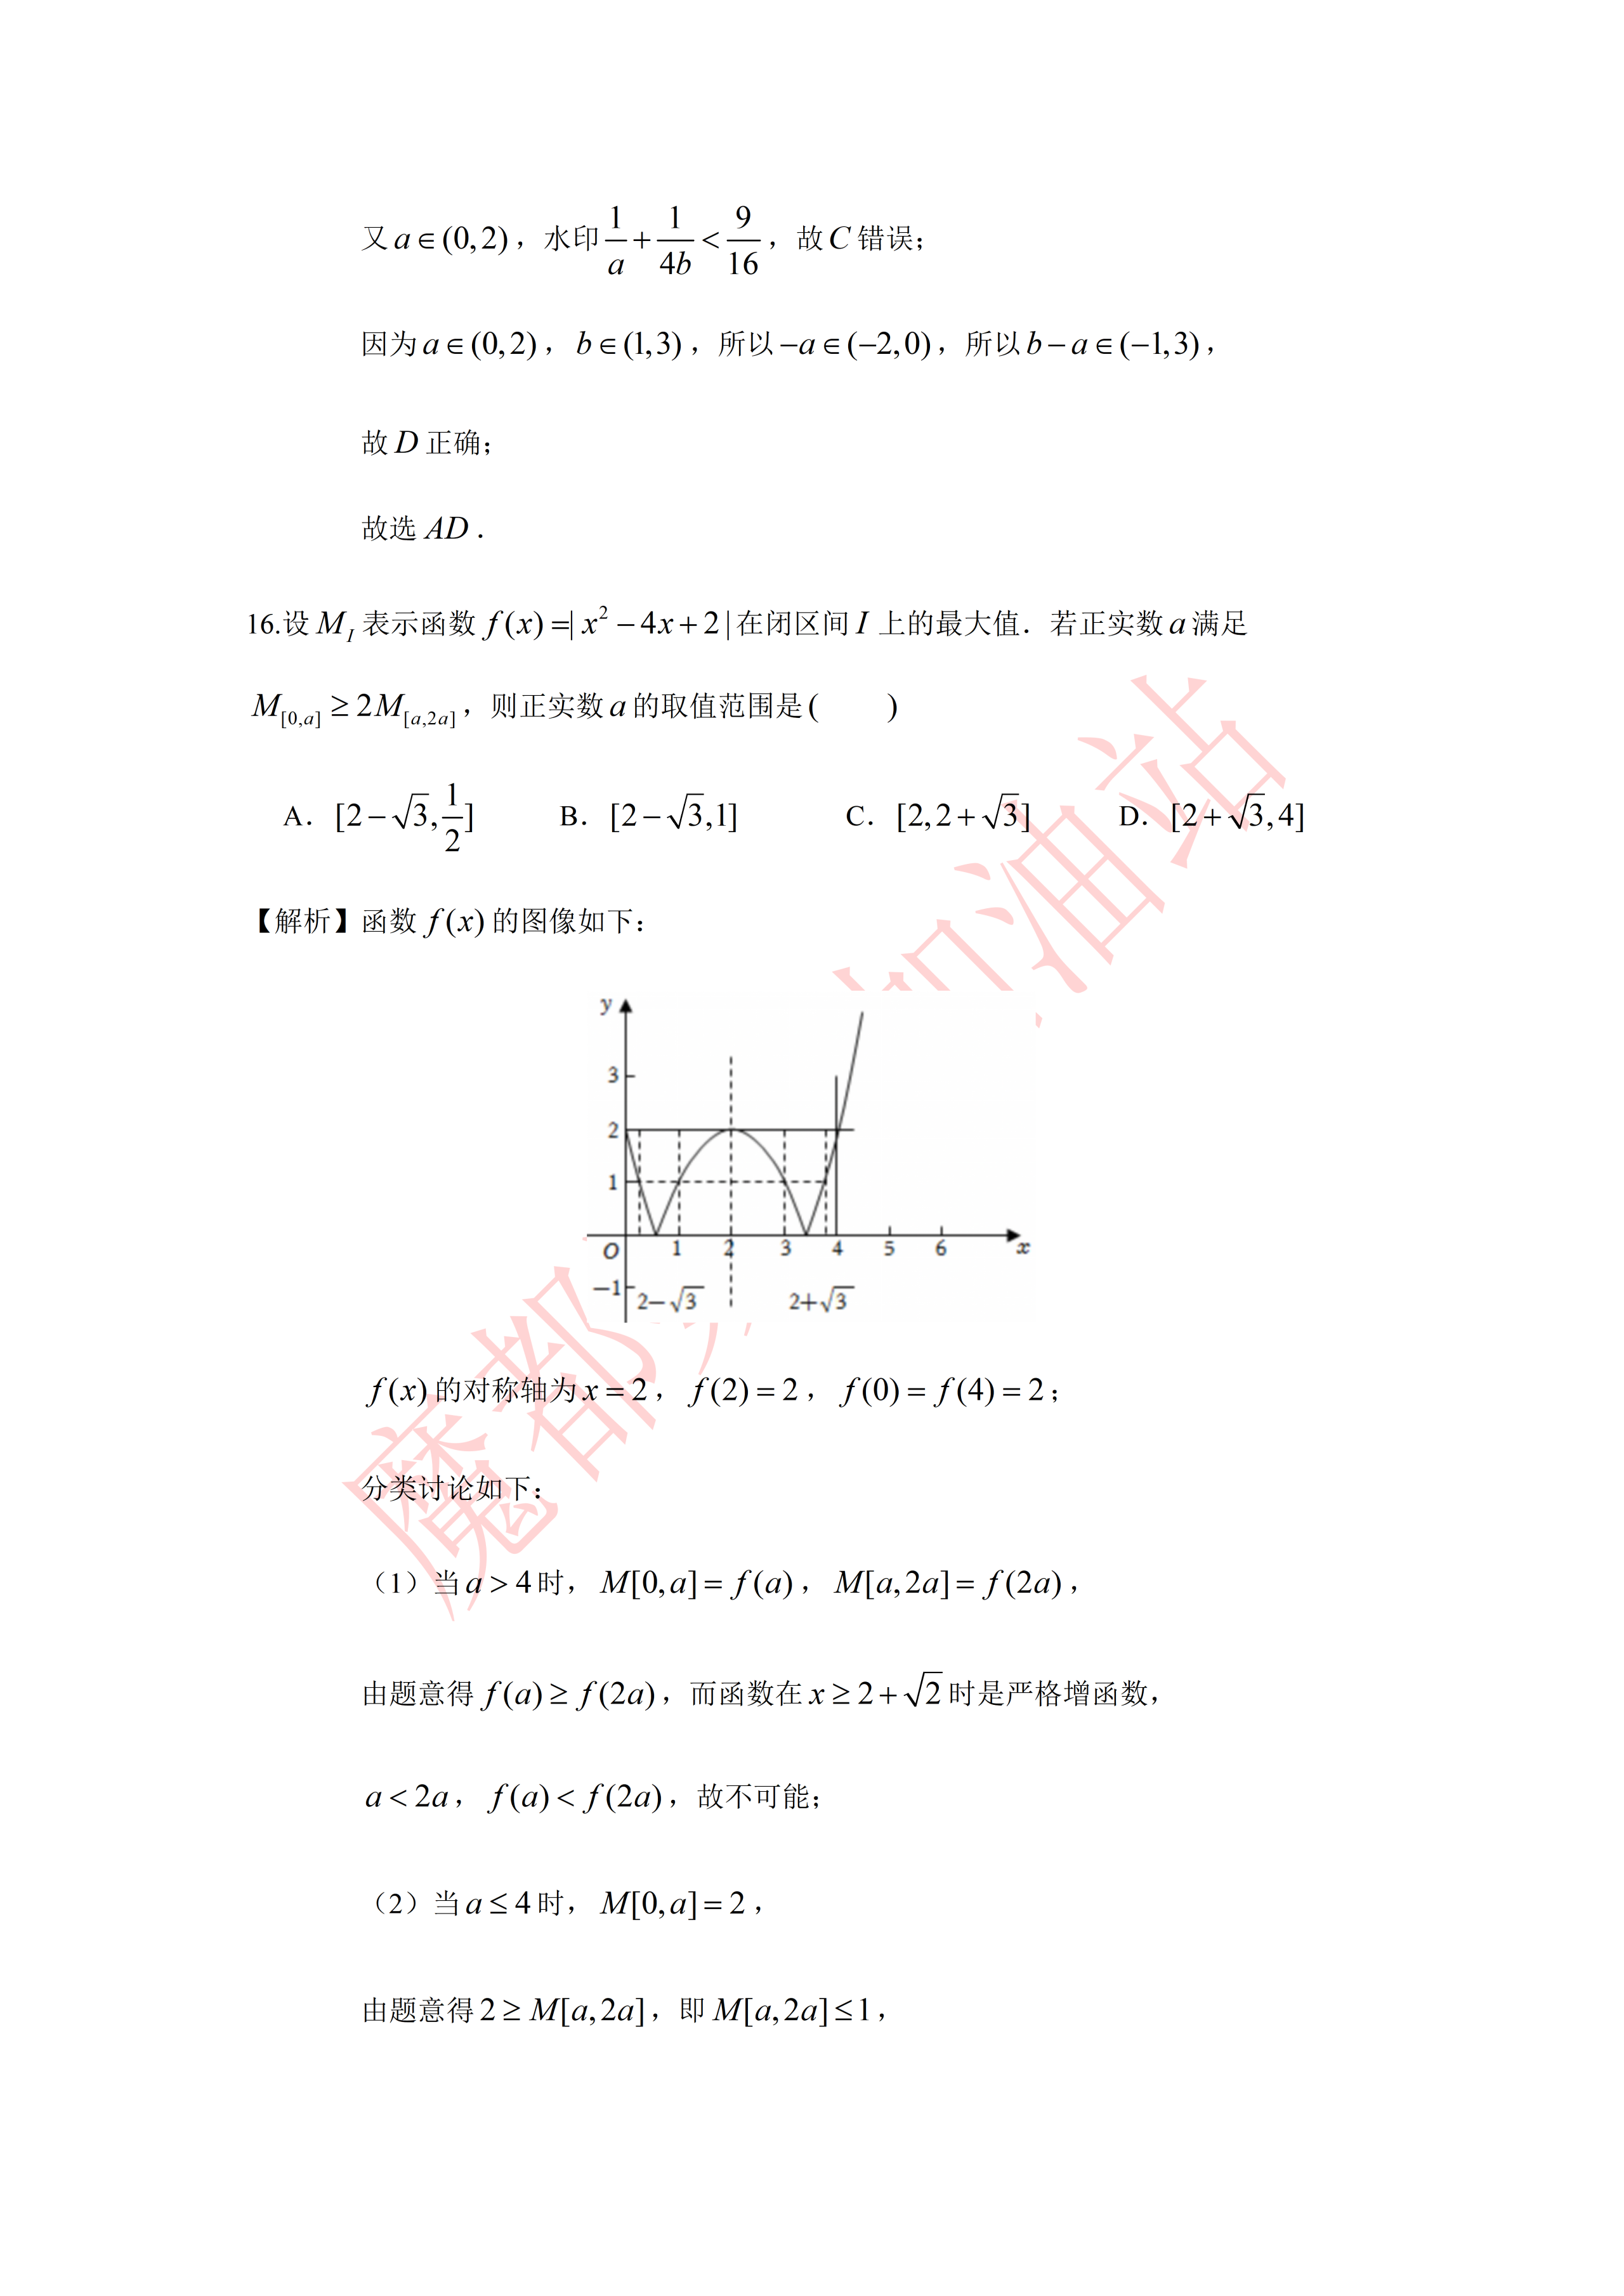
\includegraphics[width=.55\linewidth,trim=895bp 1535bp 915bp 1525bp,clip]{../原图/高一51_华师大二附中_国庆作业3/06.png}
\end{center}
\step{$f(x)$ 的对称轴为 $x=2$，$f(2)=2$，$f(0)=f(4)=2$；}
\step{分类讨论如下：}
\stepm{(1)}{当 $a>4$ 时，$M_{[0,a]}=f(a)$，$M_{[a,2a]}=f(2a)$，}
\step{由题意得 $f(a)\geqslant f(2a)$，而函数在 $x\geqslant2+\sqrt2$ 时是严格增函数，}
\step{$a<2a$，$f(a)<f(2a)$，故不可能；}
\stepm{(2)}{当 $a\leqslant4$ 时，$M_{[0,a]}=2$，}
\step{由题意得 $2\geqslant M_{[a,2a]}$，即 $M_{[a,2a]}\leqslant1$，}
\step{令 $f(x)=1$，解得 $x_1=2-\sqrt3$，$x_2=1$，$x_3=2+\sqrt3$，$x_4=3$，}
\step{则有 $a\geqslant2-\sqrt3$ 并且 $2a\leqslant1$，解得 $2-\sqrt3\leqslant a\leqslant\dfrac12$；}
\step{或者 $a\geqslant3$ 并且 $2a\leqslant2+\sqrt3$，无解；}
\step{故选 $A$.}
\solend

\fi

\end{enumerate}

\bigsec{三、解答题}

\begin{enumerate}
\setcounter{enumi}{16}

\item 已知 $M=\{x\mid2\leqslant x\leqslant5\}$，$N=\{x\mid a-1\leqslant x\leqslant2a+1\}$.
\begin{enumerate}[label=(\arabic*)]
\item 若 $M\subseteq N$，求实数 $a$ 的取值范围；
\item 若 $M\supseteq N$，求实数 $a$ 的取值范围.
\end{enumerate}

\ifanswer
\ans{（1）$[2,3]$；（2）$(-\infty,-2)$}
\fi

\ansspace[6]

\item 设集合 $A=\{x\mid|x+1|\leqslant3\}$，$B=\{x\mid0<x<3m\}$.
\begin{enumerate}[label=(\arabic*)]
\item 若 $A\cup B=A$，求实数 $m$ 的取值范围；
\item 设 $P=(\complement_R A)\cap B$，若 $\exists x\in\Z$ 且 $x\in P$，求实数 $m$ 的取值范围.
\end{enumerate}

\ifanswer
\solbegin
\stepm{(1)}{$A=\{x\mid|x+1|\leqslant3\}=\{x\mid-4\leqslant x\leqslant2\}$，且 $A\cup B=A$，所以 $B\subseteq A$.}
\step{若 $B=\varnothing$，此时 $0\geqslant3m$，解得 $m\leqslant0$；}
\step{若 $B\neq\varnothing$，此时 $0<3m$，且 $3m\leqslant2$，解得 $0<m\leqslant\dfrac23$；}
\step{则实数 $m$ 的取值范围是 $\left(-\infty,\dfrac23\right]$.}
\stepm{(2)}{因为 $\exists x\in\Z$ 且 $x\in P$，所以集合 $P$ 中至少存在一个整数.}
\step{$\complement_R A=\{x\mid x<-4\text{ 或 }x>2\}$，$B=\{x\mid0<x<3m\}$，}
\step{要使 $P=(\complement_R A)\cap B$ 中至少存在一个整数，则 $\begin{cases}3m>0\\3m>3\end{cases}$，解得 $m>1$，}
\step{则实数 $m$ 的取值范围是 $(1,+\infty)$.}
\solend

\fi

\ansspace[7]

\item 已知函数 $f(x)=x^2+(1-a)x-a(a\in\R)$.
\begin{enumerate}[label=(\arabic*)]
\item 解关于 $x$ 的不等式 $f(x)<0$；
\item 若 $\forall a\in[-1,1]$，$f(x)\geqslant0$ 恒成立，求实数 $x$ 的取值范围.
\end{enumerate}

\ifanswer
\solbegin
\stepm{(1)}{不等式 $x^2+(1-a)x-a<0$ 等价于 $(x-a)(x+1)<0$，}
\step{当 $a<-1$ 时，不等式的解集为 $(a,-1)$；}
\step{当 $a=-1$ 时，不等式的解集为 $\varnothing$；}
\step{当 $a>-1$ 时，不等式的解集为 $(-1,a)$.}
\stepm{(2)}{$x^2+(1-a)x-a=-a(x+1)+x^2+x$，}
\step{设 $g(a)=-a(x+1)+x^2+x$，$a\in[-1,1]$，}
\step{要使 $g(a)\geqslant0$ 在 $a\in[-1,1]$ 上恒成立，}
\step{只需 $\begin{cases}g(-1)\geqslant0\\g(1)\geqslant0\end{cases}$，即 $\begin{cases}x^2+2x+1\geqslant0\\x^2-1\geqslant0\end{cases}$，解得 $x\geqslant1$ 或 $x\leqslant-1$，}
\step{所以 $x$ 的取值范围为 $\{x\mid x\leqslant-1\text{ 或 }x\geqslant1\}$.}
\solend

\fi

\ansspace[7]

\item 若实数 $x$、$y$、$m$ 满足 $|x-m|>|y-m|$，则称 $x$ 比 $y$ 远离 $m$.
\begin{enumerate}[label=(\arabic*)]
\item 若 $2$ 比 $3x-4$ 远离 $1$，求 $x$ 的取值范围；
\item 设 $y=\dfrac{x+2}{x+1}$，其中 $x\in(0,\sqrt2)\cup(\sqrt2,+\infty)$，判断：$x$ 与 $y$ 哪一个更远离 $\sqrt2$？并说明理由.
\item 若 $x+y=2$，试问：$y$ 与 $x^2+y^2$ 哪一个更远离 $\dfrac12$？并说明理由.
\end{enumerate}

\ifanswer
\solbegin
\stepm{(1)}{由题意得 $|2-1|>|3x-4-1|$，所以 $|3x-5|<1$，解得 $\dfrac43<x<2$，}
\step{故 $x$ 的取值范围为 $\left(\dfrac43,2\right)$；}
\stepm{(2)}{$x$ 比 $y$ 更远离 $\sqrt2$，}
\step{理由如下：要证 $x$ 比 $y$ 更远离 $\sqrt2$，只要证 $|x-\sqrt2|>\left|\dfrac{x+2}{x+1}-\sqrt2\right|$，}
\step{即证 $|x-\sqrt2|>\left|\dfrac{(1-\sqrt2)(x-\sqrt2)}{x+1}\right|$，}
\step{因为 $x\in(0,\sqrt2)\cup(\sqrt2,+\infty)$，所以 $|x-\sqrt2|>0$，}
\step{所以只要证 $1>\dfrac{\sqrt2-1}{|x+1|}$，即证 $|x+1|>\sqrt2-1$，}
\step{因为 $x\in(0,\sqrt2)\cup(\sqrt2,+\infty)$，所以 $x+1\in(1,\sqrt2+1)\cup(\sqrt2+1,+\infty)$，}
\step{所以 $|x+1|>1>\sqrt2-1$，所以 $x$ 比 $y$ 更远离 $\sqrt2$；}
\stepm{(3)}{因为 $x^2+y^2\geqslant\dfrac{(x+y)^2}{2}=2$，当且仅当 $x=y=1$ 时等号成立，}
\step{所以 $\left|x^2+y^2-\dfrac12\right|=x^2+y^2-\dfrac12$，}
\step{从而 $\left|y-\dfrac12\right|-\left|x^2+y^2-\dfrac12\right|=\left|y-\dfrac12\right|-\left(x^2+y^2-\dfrac12\right)$，}
\step{①$y\geqslant\dfrac12$，$\left|y-\dfrac12\right|-\left|x^2+y^2-\dfrac12\right|=y-\dfrac12-\left(x^2+y^2-\dfrac12\right)=y-x^2-y^2$}
\step{$=y-(2-y)^2-y^2=-2y^2+5y-4=-2\left(y-\dfrac54\right)^2-\dfrac78<0$，}
\step{即 $\left|y-\dfrac12\right|<\left|x^2+y^2-\dfrac12\right|$；}
\step{②$y<\dfrac12$，}
\step{$\left|y-\dfrac12\right|-\left|x^2+y^2-\dfrac12\right|=\left(\dfrac12-y\right)-\left(x^2+y^2-\dfrac12\right)=-y-x^2-y^2+1$}
\step{$=-y-(2-y)^2-y^2+1=-2y^2+3y-3=-2\left(y-\dfrac34\right)^2-\dfrac{15}8<0$，}
\step{即 $\left|y-\dfrac12\right|<\left|x^2+y^2-\dfrac12\right|$；}
\step{综上，$\left|y-\dfrac12\right|<\left|x^2+y^2-\dfrac12\right|$，即 $x^2+y^2$ 比 $y$ 更远离 $\dfrac12$.}
\solend

\fi

\ansspace[9]

\item 对于非空有限整数集 $X$，$m\in\N^*$，定义 $X^m=\{x^m\mid x\in X\}$，对 $n\in\Z$，
$Y\oplus n=\{x+n\mid x\in Y\}$ 现有两个非空有限整数集 $A$、$B$，已知 $A\oplus1\subseteq B$ 且
$B^2\oplus(-4)\subseteq A$.
\begin{enumerate}[label=(\arabic*)]
\item 当 $A=\{-3,0\}$ 时求集合 $B$；
\item 证明：$A\subseteq\{-3,-2,0,1\}$；
\item 当 $A\oplus1=B$ 且 $B^2\oplus(-4)=A$ 时，任取 $a\in A$，$b\in B$ 构造函数
$f(x)=(x-a)(x-b)$ 问：当 $a$、$b$ 取何值时，$f(x)$ 的最小值最小？
\end{enumerate}

\ifanswer
\solbegin
\stepm{(1)}{因为 $A=\{-3,0\}$，$B^2\oplus(-4)\subseteq A$，}
\step{所以 $B^2\oplus(-4)$ 可能为 $\varnothing$、$\{-3\}$、$\{0\}$、$\{-3,0\}$，}
\step{当 $B^2\oplus(-4)=\varnothing$ 时 $B^2=\varnothing$，不满足非空，不合题意；}
\step{当 $B^2\oplus(-4)=\{-3\}$ 时 $B^2=\{1\}$，所以 $B=\{1,-1\}$、$\{1\}$、$\{-1\}$，}
\step{当 $B^2\oplus(-4)=\{0\}$ 时 $B^2=\{4\}$，所以 $B=\{2,-2\}$、$\{2\}$、$\{-2\}$，}
% 原卷如此，照录未改（此处作 $\{0,-3\}$，上一行同一集合作 $\{-3,0\}$）
\step{当 $B^2\oplus(-4)=\{0,-3\}$ 时 $B^2=\{4,1\}$，}
\step{所以 $B=\{1,2,-1,-2\}$、$\{2,-1,-2\}$、$\{2,1,-2\}$、$\{1,-1,-2\}$、$\{1,-1,2\}$、$\{1,2\}$、$\{-1,2\}$、$\{-1,-2\}$、$\{1,-2\}$，}
\step{又 $A\oplus1=\{-2,1\}\subseteq B$，得 $B$ 为 $\{1,-2\}$、$\{2,1,-2\}$、$\{1,-1,-2\}$、$\{1,2,-1,-2\}$.}
\stepm{(2)}{设 $x\in A$，因为 $A\oplus1\subseteq B$，所以 $x+1\in B$，}
\step{又 $B^2\oplus(-4)\subseteq A$，所以 $(x+1)^2-4\in A$，}
% 原卷如此，照录未改（此处及下文取 $x=2$ 处原卷均作 $(-4+1)^2-4=52-2a>0$）
\step{取 $x=-4$，则 $(-4+1)^2-4=52-2a>0$，$(5+1)^2-4=32\in A$，$\cdots$，}
\step{无限迭代，而 $A$ 为有限集，不合题意，舍去，即 $-4\notin A$；}
\step{取 $x=-3$，则 $(-3+1)^2-4=0\in A$，$(0+1)^2-4=-3\in A$，}
\step{得 $A$ 集合可为 $\{-3,0\}$；}
\step{取 $x=-2$，则 $(-2+1)^2-4=-3\in A$，$(-3+1)^2-4=0\in A$，}
\step{$(0+1)^2-4=-3\in A$，得 $A$ 集合可为 $\{-3,-2,0\}$；}
\step{取 $x=-1$，则 $(-1+1)^2-4=-4\in A$，又 $-4\notin A$，所以 $-1\notin A$，}
\step{取 $x=1$，则 $(1+1)^2-4=0\in A$，$(0+1)^2-4=-3\in A$，}
\step{$(-3+1)^2-4=0\in A$，得 $A$ 集合可为 $\{-3,0,1\}$，}
\step{取 $x=2$，则 $(2+1)^2-4=52-2a>0$，$(5+1)^2-4=32\in A$，$\cdots$，}
\step{无限迭代，而 $A$ 为有限集，不合题意，舍去，即 $2\notin A$，}
\step{同理当 $x<-4$ 或 $x>2$，且 $x\in\Z$ 时不符合 $A$ 为有限集，舍去；}
\step{故由上得 $A$ 集合可为 $\{-3,0\},\{-3,-2,0\},\{-3,0,1\},\{-3,-2,0,1\}$，}
\step{所以 $A\subseteq\{-3,-2,0,1\}$，}
\stepm{(3)}{当 $A\oplus1=B$ 且 $B^2\oplus(-4)=A$ 时，}
\step{设 $x\in B$，则 $x^2-4\in B^2\oplus(-4)=A$，}
% 原卷如此，照录未改（题设 $A=\{-3,0\}$，此处两个判别式取的是 $-2$ 与 $1$，均不属于 $A$）
\step{$x^2-4=-2$ 时 $x=\pm\sqrt2$，不为整数，不合题意；}
\step{$x^2-4=1$ 时 $x=\pm\sqrt5$，不为整数，不合题意；}
\step{所以 $A=\{-3,0\}$，又 $A\oplus1=B$，则 $B=\{-2,1\}$，}
\step{任取 $a\in A$，$b\in B$ 构造函数 $f(x)=(x-a)(x-b)$，}
\step{$f(x)=(x-a)(x-b)=x^2-(a+b)x+ab$}
\step{$=x^2-(a+b)x+\dfrac{(a+b)^2}{4}+ab-\dfrac{(a+b)^2}{4}$}
\step{$=\left[x-\dfrac{(a+b)}2\right]^2-\dfrac{(a-b)^2}{4}\geqslant-\dfrac{(a-b)^2}{4}$，所以 $f(x)_{min}=-\dfrac{(a-b)^2}{4}$，}
\step{又 $a\in A=\{-3,0\}$，$b\in B=\{-2,1\}$，所以 $a-b$ 的取值有 $-1,-4,2$，}
\step{所以 $f(x)_{min}=-\dfrac{(a-b)^2}{4}\geqslant-\dfrac{(-3-1)^2}{4}=-4$，}
\step{即当 $a=-3$，$b=1$ 时 $f(x)_{min}$ 的最小值为 $-4$.}
\solend

\fi

\ansspace*[12]

\end{enumerate}

\end{document}
"
%
% 原始材料：微信公众号“魔都数学加油站”文章，作者破晓，连载“27学年高一51”；
% 原文标题“27学年高一51——2026-2027年上海市华师大二附中高一上国庆作业3”；
% 原文链接：https://mp.weixin.qq.com/s/95SLMEmPUT30s4U7wjr5Og。
% 该页面用 JS 渲染，未见明确发布日期；页面内时间戳约为 2026-10-05 21:37，本稿以该时刻记可得日期。
% 正文为 12 张 PNG 页：第 01、02、03、05、07、08、11 页 4762×6735，
% 第 04、06、09、10、12 页 2560×3620。按页序逐页读取，12 页全为试卷正文页
% （卷首标题在第 1 页页顶，卷末解答题止于第 12 页），无封面页、目录页或单独的页脚页。
% 卷面标题照原卷印作“2026-2027 年华师大二附中高一上国庆作业 3”（公众号标题中的“上海市”
% 卷面标题行没有，本稿照卷面），年份区间按全稿惯例排 en dash。
%
% 篇幅与题号：原卷自第 3 题起编号（第 1、2 题不在本卷内）。填空题 3—12（10 题）、
% 选择题 13—16（4 题）、解答题 17—21（5 题），共 19 题。本稿沿用原节与原题号，
% 只改排为全稿统一的大节样式（原卷小节标题为“一、填空题”“二、选择题”“三、解答题”）。
% 正文为讲评版：填空题 3—12 与选择题 13—16 只印【解析】（选择题的结论“故选 X”印在解析内），
% 按全稿口径这类题不另提 \ans{}；解答题第 17 题只印【答案】，故只给 \ans{}；
% 第 18—21 题只印【解析】。
%
% 副标题：原卷未印副标题。本稿按“知识模块”口径标作“集合与常用逻辑用语、不等式”：
% 19 题中集合与常用逻辑用语 8 题（3、4、6、10、13、17、18、21），
% 不等式（含函数最值、绝对值不等式）11 题（5、7、8、9、11、12、14、15、16、19、20），
% 两类均远超三分之一，故并标。口径同 高一46_交附闵行_国庆作业3、高一48_华师大二附中_周末作业2。
%
% 与原卷的排版差异：
%   ① 原卷每题下直接印【答案】或【解析】，本稿按全稿惯例将答案与解析置于答案版；
%   ② 原卷未印副标题，本稿按“知识模块”口径补出；
%   ③ 原卷填空横线按全稿惯例排为 \blankline[4.4em]；
%   ④ 原卷 $R$、$N$、$Z$ 均排斜体，本稿按全稿惯例改用花体 $\R$、$\N$、$\Z$（同 高一48）；
%   ⑤ 原卷第 12 题解析配图、第 13 题题干韦恩图都印在正文右侧的浮动位置，第 16 题解析配图
%      印在解析行间；本稿三图一律居中排，均自原图对应页裁切（trim），不另存图片文件；
%   ⑥ 原卷解答题未留作答空白，本稿按全稿惯例加 \ansspace；
%   ⑦ 原卷第 15 题解析第 7、8 两个印刷行是一串连等式的折行，本稿按“一条 \step ＝ 一个印刷行”
%      的口径分成两条 \step。
%
% 原卷笔误/存疑（均照录未改，正文对应处另有 % 注）：
%   ① 第 12 题解析末行作“区间长度之和为 $x_1-b+x_2-a=x_1-x_2-a-b=2+a+b-a-b=2$”，
%      按上一行 $x_1+x_2=2+a+b$，此处应为 $x_1+x_2$；原卷作 $x_1-x_2$。
%   ② 第 15 题解析“又 $a\in(0,2)$，”与 $\dfrac1a+\dfrac1{4b}<\dfrac9{16}$ 之间，
%      原卷正文夹印“水印”二字（系制版遗留字样，非试卷内容）。
%   ③ 第 21 题第 (2) 问解析两处（取 $x=-4$、取 $x=2$）作“$=52-2a>0$”，
%      与题设 $(x+1)^2-4$ 的取值（按 $x=-4$ 应为 $5$）不符，当系原卷算式遗留。
%   ④ 第 21 题第 (1) 问解析先写 $B^2\oplus(-4)$ 可能为 $\{-3,0\}$，后文又作 $\{0,-3\}$，
%      同一集合两种写法。
%   ⑤ 第 21 题第 (3) 问解析：题设 $B^2\oplus(-4)=A$ 且 $A=\{-3,0\}$ 时，由 $x^2-4\in A$
%      应得 $x^2-4=-3$ 或 $0$；原卷讨论的却是 $x^2-4=-2$ 与 $x^2-4=1$（两值均不属于 $A$），
%      与题设不合。
%
% 插图：3 张，均自原图裁切（无 \begin{tikzpicture} 重排）：
%   · 第 13 题题干韦恩图（原图第 04 页，图在题干与选项右侧）
%   · 第 12 题解析配图（原图第 04 页，图在解析右侧）
%   · 第 16 题解析配图（原图第 06 页，图在解析中间）
%
\documentclass[a4paper,11pt]{article}
\usepackage{common}

\begin{document}

\examtitlest[3]{2026--2027 年华师大二附中高一上国庆作业 3}{集合与常用逻辑用语、不等式}

\bigsec{一、填空题}

\begin{enumerate}
\setcounter{enumi}{2}

\item 若 $\{x\mid x<1\text{ 或 }x>4\}\cup\{x\mid m<x<2m+3\}=R$，则实数 $m$ 的取值范围为\blankline[4.4em].

\ifanswer
\solbegin
\step{因为 $\{x\mid x<1\text{ 或 }x>4\}\cup\{x\mid m<x<2m+3\}=R$，}
\step{所以 $\begin{cases}m<1\\2m+3>4\end{cases}$，解得 $\dfrac12<m<1$，所以 $m$ 的取值范围为 $\left(\dfrac12,1\right)$.}
\solend

\fi

\item 若“$x\leqslant5$”是“$x<a$”的必要不充分条件，则 $a$ 的取值范围是\blankline[4.4em].

\ifanswer
\solbegin
\step{若“$x\leqslant5$”是“$x<a$”的必要不充分条件，则 $\{x\mid x<a\}\subset\{x\mid x\leqslant5\}$，}
\step{所以 $a\leqslant5$.}
\solend

\fi

\item 实数 $x$、$y$ 满足 $x^2+2xy+4y^2=1$，则 $x+2y$ 的取值范围是\blankline[4.4em].

\ifanswer
\solbegin
\step{因为 $x^2+2xy+4y^2=(x+2y)^2-2xy=1$，}
\step{所以 $(x+2y)^2-1=x\cdot(2y)\leqslant\left(\dfrac{x+2y}{2}\right)^2$，当且仅当 $x=2y$ 时取等号，}
\step{解得 $-\dfrac{2\sqrt3}{3}\leqslant x+2y\leqslant\dfrac{2\sqrt3}{3}$，故 $x+2y$ 的取值范围是 $\left[-\dfrac{2\sqrt3}{3},\dfrac{2\sqrt3}{3}\right]$.}
\solend

\fi

\item 若命题 $p$：“$\exists x\in\R$，$5x^2-3x+m=0$”为假命题，则实数 $m$ 的取值范围为\blankline[4.4em].

\ifanswer
\solbegin
\step{若命题 $p$：$\exists x\in\R$，$5x^2-3x+m=0$ 为假命题，}
\step{则 $5x^2-3x+m=0$ 没有实数根，故 $\Delta=9-20m<0$，解得 $m>\dfrac9{20}$.}
\solend

\fi

\item 若当 $3\leqslant m\leqslant5$ 时，$mx^2-mx+m-9<0$ 有解，则实数 $x$ 的取值范围是\blankline[4.4em].

\ifanswer
\solbegin
\step{当 $3\leqslant m\leqslant5$ 时，$mx^2-mx+m-9<0$ 有解，}
\step{即 $(x^2-x+1)m-9<0$ 在 $m\in[3,5]$ 上有解，}
\step{因为 $x^2-x+1>0$，所以一次函数 $g(m)=(x^2-x+1)m-9$ 严格增，}
\step{所以只需 $g(3)=3x^2-3x-6<0$ 即可，}
\step{即 $x^2-x-2<0$，$(x-2)(x+1)<0$，解得 $-1<x<2$，}
\step{所以实数 $x$ 的取值范围是 $(-1,2)$.}
\solend

\fi

\item 已知不等式 $\dfrac{x}{x^2+4}\leqslant a$ 对任意的 $x\in[1,3]$ 恒成立，则实数 $a$ 的范围为\blankline[4.4em].

\ifanswer
\solbegin
\step{因为 $x\in[1,3]$，所以 $\dfrac{x}{x^2+4}=\dfrac{1}{x+\dfrac4x}\leqslant\dfrac{1}{2\sqrt{x\times\dfrac4x}}=\dfrac14$，}
\step{当且仅当 $x=\dfrac4x$ 时，即 $x=2$ 时取等号，即 $\dfrac{x}{x^2+4}$ 在 $x\in[1,3]$ 的最大值为 $\dfrac14$，}
\step{又由不等式 $\dfrac{x}{x^2+4}\leqslant a$ 对任意的 $x\in[1,3]$ 恒成立，所以 $a\geqslant\dfrac14$，}
\step{即实数 $a$ 的范围为 $\left[\dfrac14,+\infty\right)$.}
\solend

\fi

\item 甲、乙两人解关于 $x$ 的不等式 $x^2+bx+c<0$，甲写错了 $b$，正确计算后得到的解为 $\{x\mid1<x<2\}$；
乙写错了 $c$，正确计算后得到的解为 $\{x\mid-4<x<1\}$. 那么不等式 $\dfrac{bx+c}{x-2}<0$ 的解为\blankline[4.4em].

\ifanswer
\solbegin
\step{由 $x^2+bx+c<0$ 的解为 $\{x\mid1<x<2\}$，}
\step{则 $1$ 和 $2$ 是方程 $x^2+bx+c=0$ 的两个根，}
\step{甲写错了 $b$，但 $c$ 是正确的，所以 $c=1\times2=2$；}
\step{由 $x^2+bx+c<0$ 的解为 $\{x\mid-4<x<1\}$，}
\step{则 $-4$ 和 $1$ 是方程 $x^2+bx+c=0$ 的两个根，}
\step{乙写错了 $c$，但 $b$ 是正确的，所以 $-b=-4+1=-3$，即 $b=3$.}
\step{由 $\dfrac{bx+c}{x-2}<0$，得 $\dfrac{3x+2}{x-2}<0$，即 $(3x+2)(x-2)<0$，解得 $-\dfrac23<x<2$.}
\step{不等式 $\dfrac{bx+c}{x-2}<0$ 的解为 $\left\{x\mid-\dfrac23<x<2\right\}$.}
\solend

\fi

\item 已知 $\dfrac{1}{x-2}\geqslant1$ 是 $|x-a|<2$ 的充分非必要条件，则实数 $a$ 的取值范围是\blankline[4.4em].

\ifanswer
\solbegin
\step{由 $\dfrac{1}{x-2}\geqslant1$ 得 $\dfrac{3-x}{x-2}\geqslant0$，解得 $2<x\leqslant3$，由 $|x-a|<2$ 得 $a-2<x<a+2$，}
\step{因为 $\dfrac{1}{x-2}\geqslant1$ 是 $|x-a|<2$ 的充分非必要条件，}
\step{所以 $\{x\mid2<x\leqslant3\}\subset\{x\mid a-2<x<a+2\}$，所以 $\begin{cases}a-2\leqslant2\\a+2>3\end{cases}$，解得 $1<a\leqslant4$，}
\step{即实数 $a$ 的取值范围是 $(1,4]$.}
\solend

\fi

\item 设 $a>0$，$b>0$，若不等式 $a(a+1)^2+b(b+1)^2\geqslant\lambda ab$ 恒成立，则实数 $\lambda$ 的最大值为\blankline[4.4em].

\ifanswer
\solbegin
\step{$a(a+1)^2+b(b+1)^2\geqslant\lambda ab\Leftrightarrow\lambda\leqslant\dfrac{a(a+1)^2+b(b+1)^2}{ab}=\dfrac{(a+1)^2}{b}+\dfrac{(b+1)^2}{a}$，}
\step{从而原问题转化为求 $\dfrac{(a+1)^2}{b}+\dfrac{(b+1)^2}{a}$ 的最小值.}
\step{因为 $\dfrac{(a+1)^2}{b}+\dfrac{(b+1)^2}{a}=\dfrac{b^2+2b+1}{a}+\dfrac{a^2+2a+1}{b}$}
\step{$=\left(\dfrac{b^2}{a}+\dfrac{a^2}{b}\right)+2\left(\dfrac ba+\dfrac ab\right)+\left(\dfrac1a+\dfrac1b\right)\geqslant2\sqrt{\dfrac{b^2}{a}\cdot\dfrac{a^2}{b}}+2\times2\sqrt{\dfrac ba\cdot\dfrac ab}+2\sqrt{\dfrac1a\cdot\dfrac1b}$}
\step{$=2\sqrt{ab}+4+\dfrac{2}{\sqrt{ab}}\geqslant2\sqrt{2\sqrt{ab}\cdot\dfrac{2}{\sqrt{ab}}}+4=8$，以上均当且仅当 $a=b$ 时取等号，}
\step{所以 $\lambda\leqslant8$，即实数 $\lambda$ 的最大值为 $8$.}
\solend

\fi

\item 定义区间 $(a,d)$、$[a,d)$、$(a,d]$、$[a,d]$ 的长度为 $d-a$（$d>a$），已知 $a>b$，则满足
$\dfrac{1}{x-a}+\dfrac{1}{x-b}\geqslant1$ 的 $x$ 构成的区间的长度之和为\blankline[4.4em].

\ifanswer
\solbegin
\step{因为 $\dfrac{1}{x-a}+\dfrac{1}{x-b}\geqslant1$，所以 $\dfrac{2x-(a+b)}{(x-a)(x-b)}\geqslant1$，}
\step{即 $\dfrac{2x-(a+b)}{(x-a)(x-b)}-1\geqslant0$，则 $\dfrac{x^2-(2+a+b)x+ab+a+b}{(x-a)(x-b)}\leqslant0$，}
\step{设 $x^2-(2+a+b)x+ab+a+b=0$ 的根为 $x_1$ 和 $x_2$，}
\begin{center}
% 原卷该图印在解析右侧（原图第 04 页），本稿移作居中排，直接裁取原图，不另存图片文件。
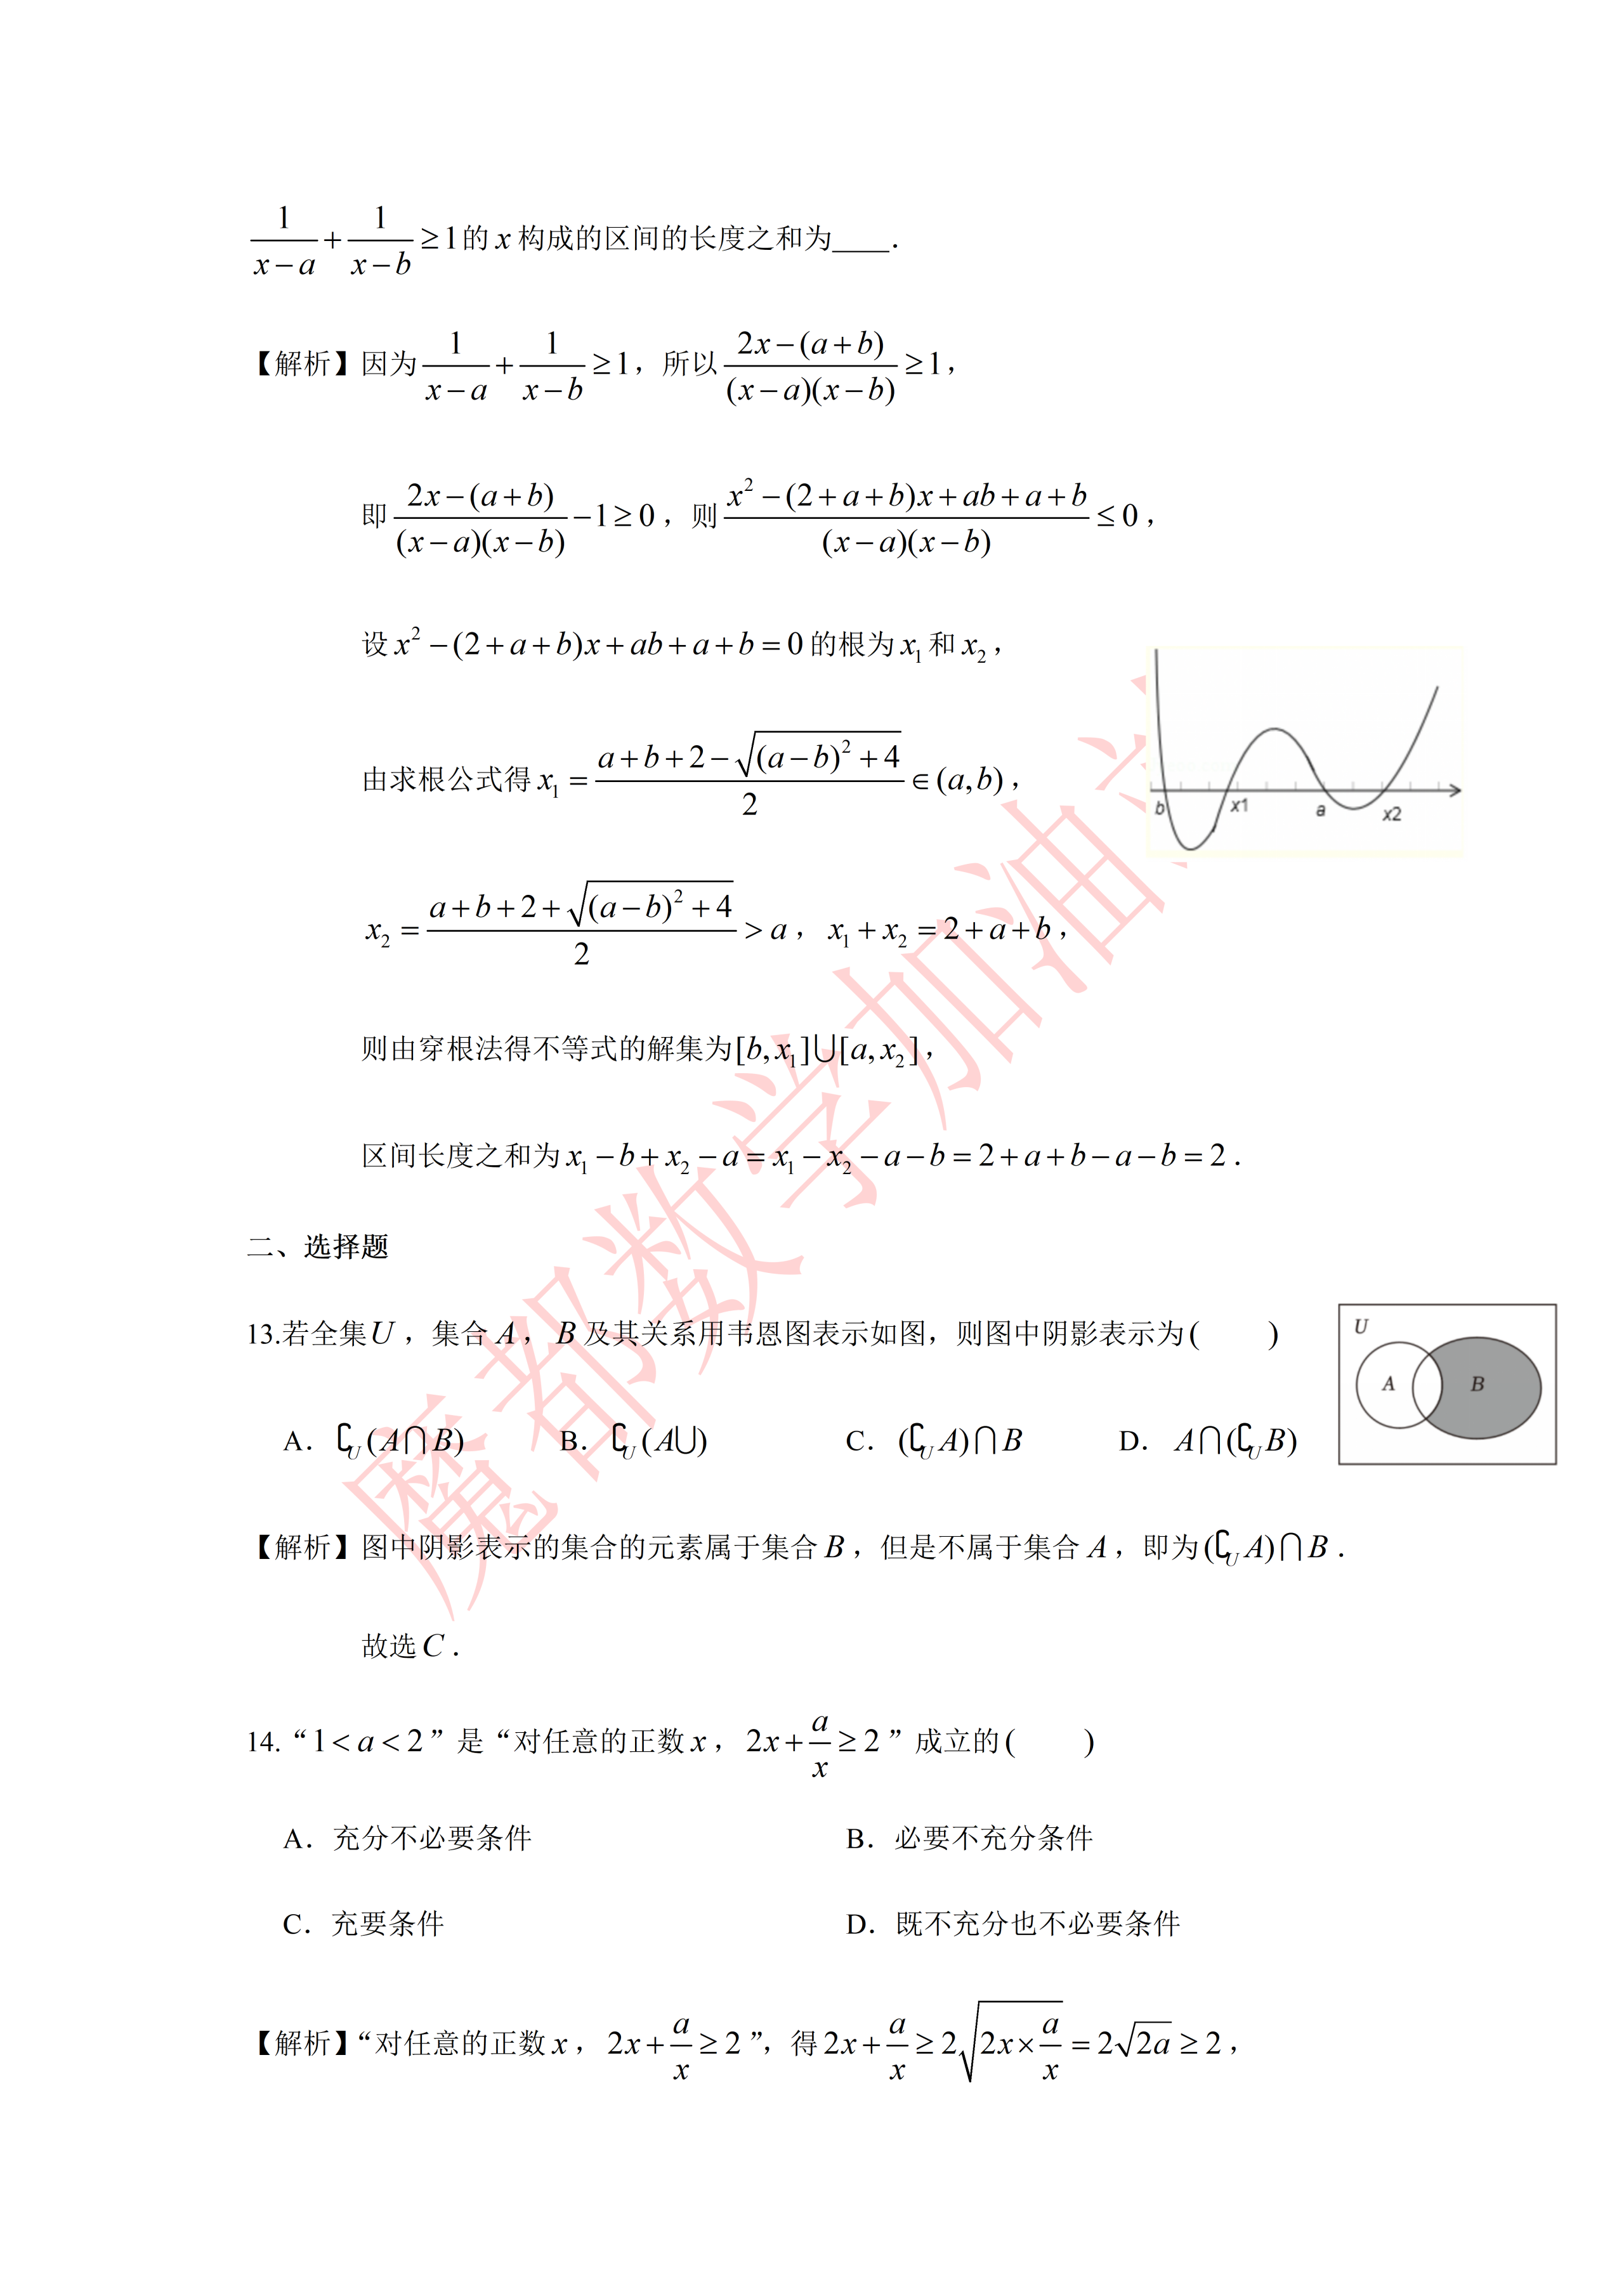
\includegraphics[width=.50\linewidth,trim=1786bp 2255bp 228bp 985bp,clip]{../原图/高一51_华师大二附中_国庆作业3/04.png}
\end{center}
\step{由求根公式得 $x_1=\dfrac{a+b+2-\sqrt{(a-b)^2+4}}{2}\in(a,b)$，}
\step{$x_2=\dfrac{a+b+2+\sqrt{(a-b)^2+4}}{2}>a$，$x_1+x_2=2+a+b$，}
\step{则由穿根法得不等式的解集为 $[b,x_1]\cup[a,x_2]$，}
% 原卷如此，照录未改（此处原卷作 $x_1-x_2$，按上一行 $x_1+x_2=2+a+b$ 当为 $x_1+x_2$）
\step{区间长度之和为 $x_1-b+x_2-a=x_1-x_2-a-b=2+a+b-a-b=2$.}
\solend

\fi

\end{enumerate}

\bigsec{二、选择题}

\begin{enumerate}
\setcounter{enumi}{12}

% 本题是“题干 + 图 + 选项”约 5.5cm 的一整块，图夹在题干与选项之间时 \keepwithprev 挡不住断点，
% 故按 高一30 第 13 题的成例在题前先量一次页高（守卫放在 \item 之前）。
\needvspace{6cm}
\item 若全集 $U$，集合 $A$、$B$ 及其关系用韦恩图表示如图，则图中阴影表示为\mbox{（\quad）}

\begin{center}
% 原卷该图印在题干与选项右侧（原图第 04 页），本稿移作居中排，直接裁取原图，不另存图片文件。
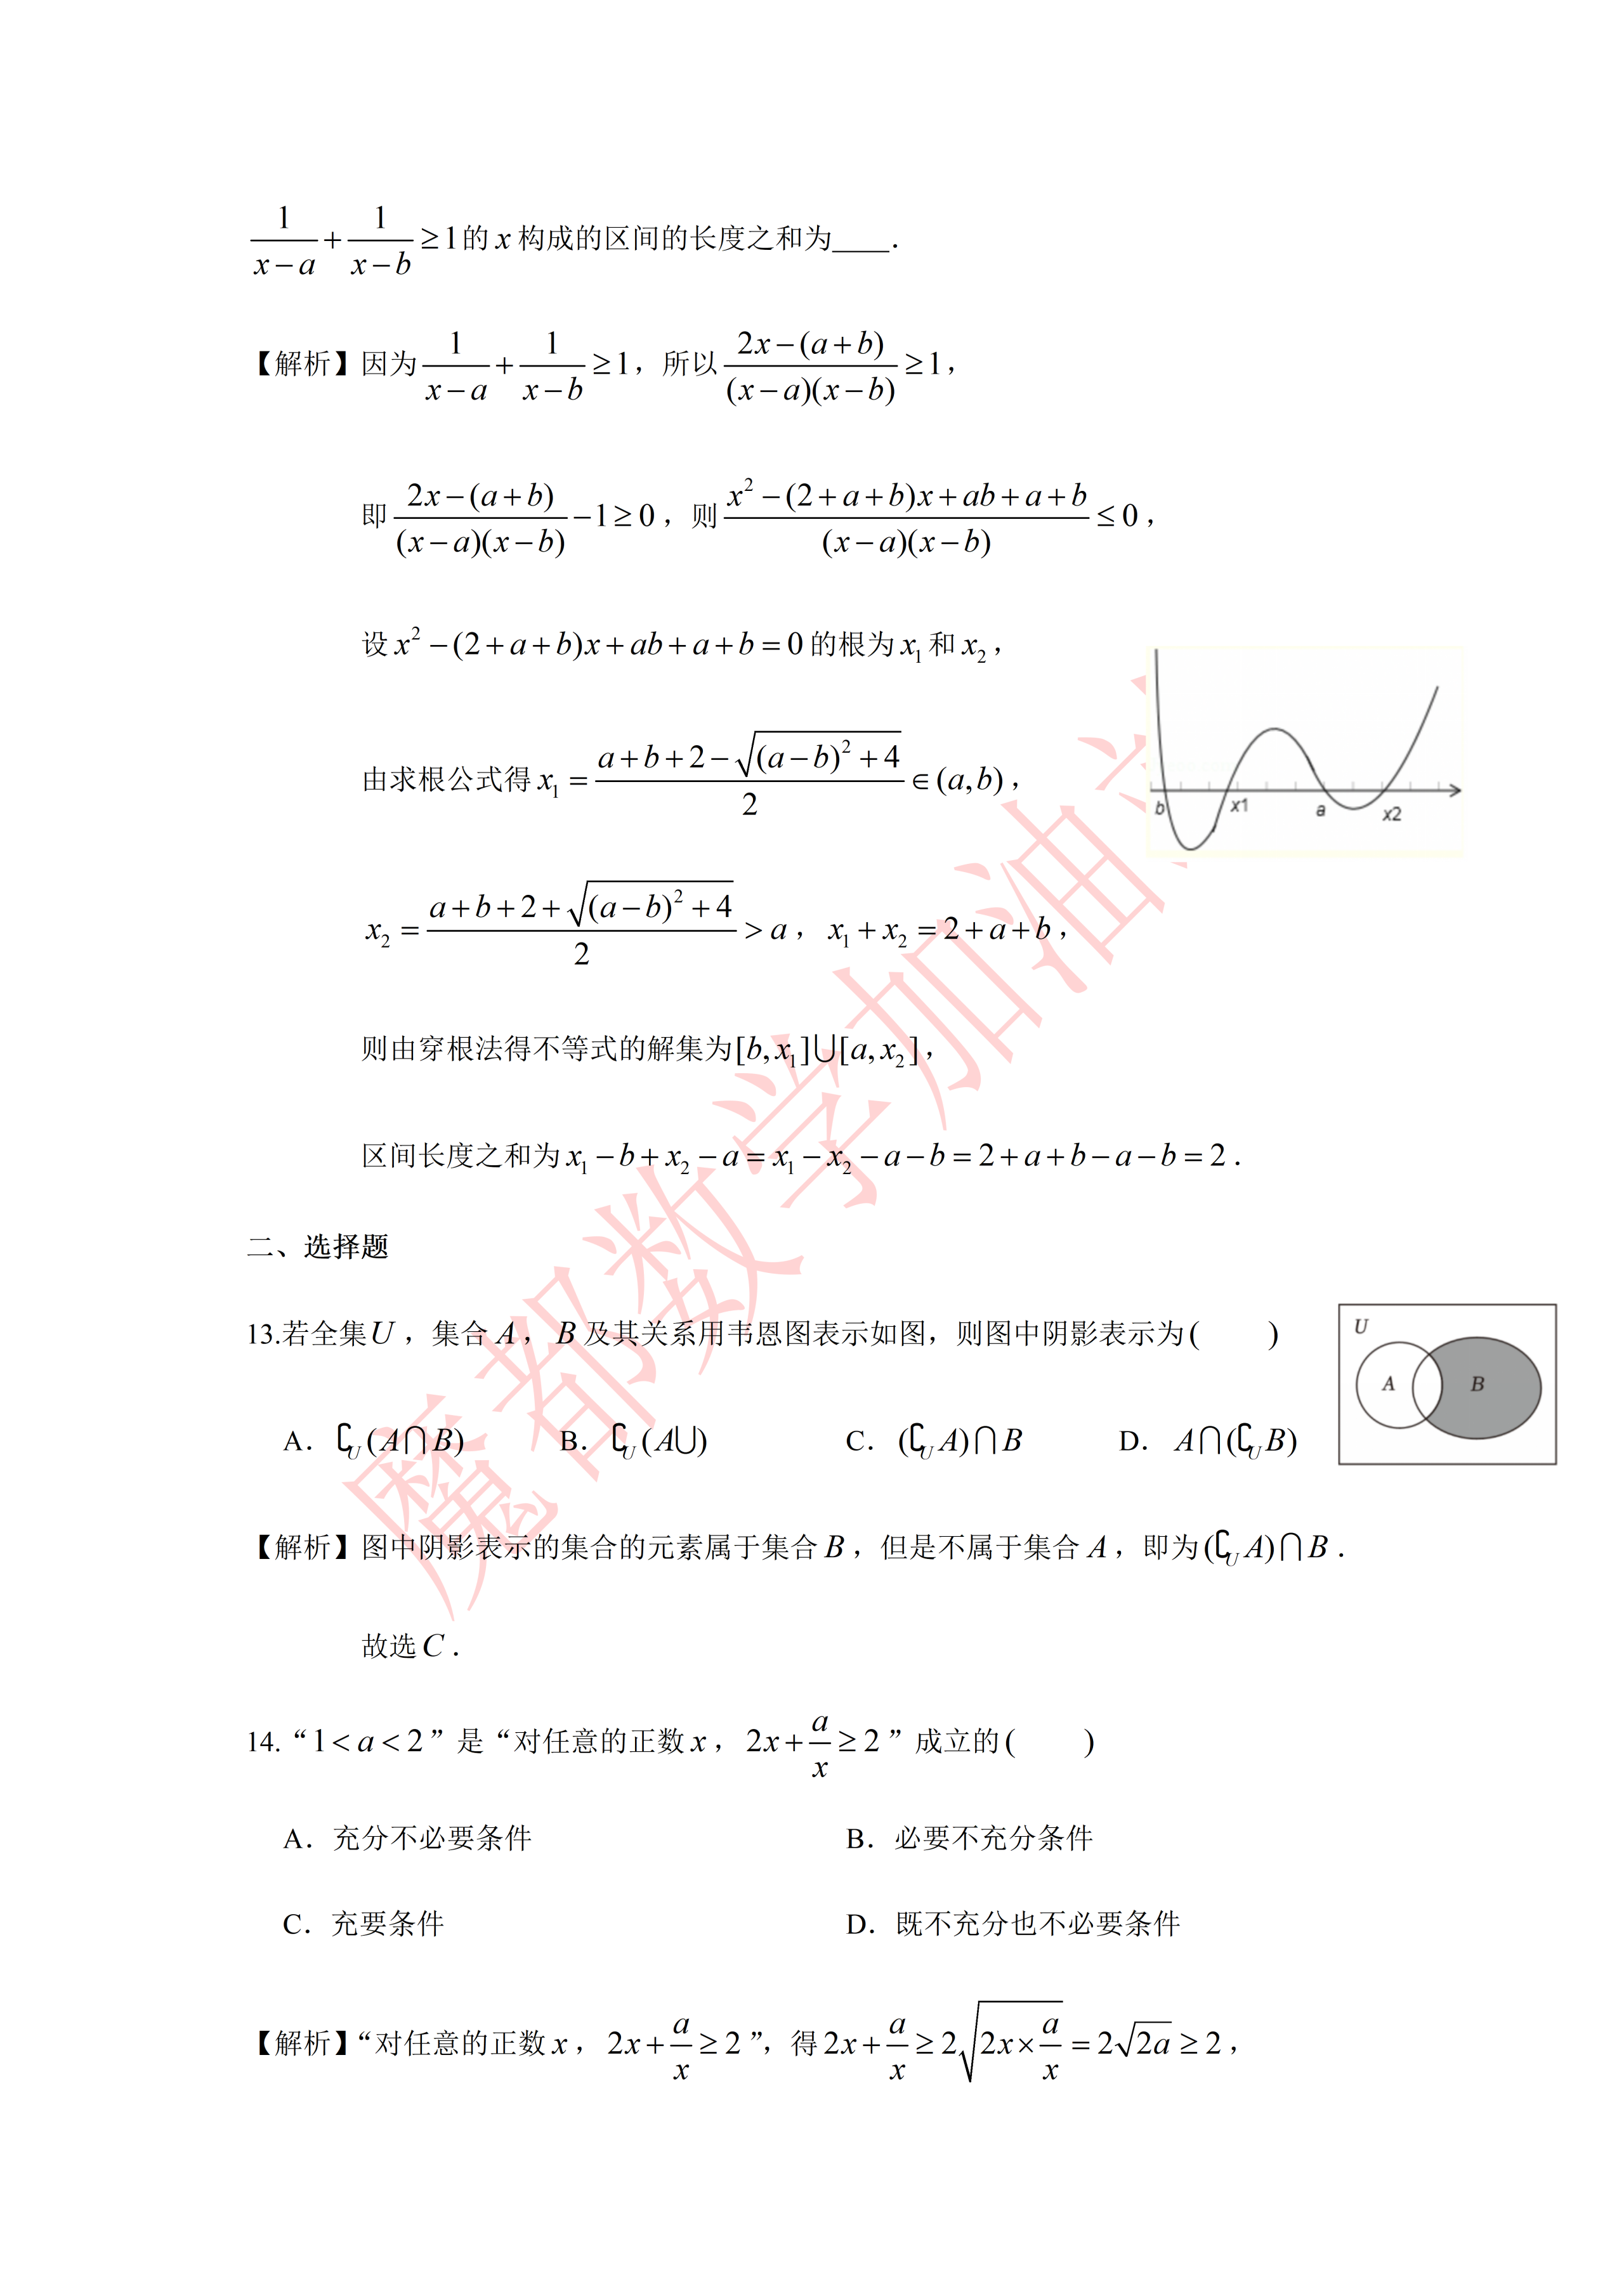
\includegraphics[width=.30\linewidth,trim=2105bp 1308bp 105bp 2050bp,clip]{../原图/高一51_华师大二附中_国庆作业3/04.png}
\end{center}

\keepwithprev
A. $\complement_U(A\cap B)$\qquad B. $\complement_U(A\cup B)$

C. $(\complement_U A)\cap B$\qquad D. $A\cap(\complement_U B)$

\ifanswer
\solbegin
\step{图中阴影表示的集合的元素属于集合 $B$，但是不属于集合 $A$，即为 $(\complement_U A)\cap B$.}
\step{故选 $C$.}
\solend

\fi

\item “$1<a<2$”是“对任意的正数 $x$，$2x+\dfrac ax\geqslant2$”成立的\mbox{（\quad）}

\keepwithprev
A. 充分不必要条件\qquad B. 必要不充分条件

C. 充要条件\qquad\qquad D. 既不充分也不必要条件

\ifanswer
\solbegin
\step{“对任意的正数 $x$，$2x+\dfrac ax\geqslant2$”，得 $2x+\dfrac ax\geqslant2\sqrt{2x\times\dfrac ax}=2\sqrt{2a}\geqslant2$，}
\step{所以 $\sqrt{2a}\geqslant1$，解得 $a\geqslant\dfrac12$，}
\step{若“$1<a<2$”得 $2x+\dfrac ax\geqslant2\sqrt{2x\times\dfrac ax}=2\sqrt{2a}>2\sqrt2>2$，}
\step{所以“$1<a<2$”$\Rightarrow$“对任意的正数 $x$，$2x+\dfrac ax\geqslant2$”，}
\step{所以“$1<a<2$”是“对任意的正数 $x$，$2x+\dfrac ax\geqslant2$”成立的充分不必要条件，}
\step{故选 $A$.}
\solend

\fi

\item 已知函数 $f(x)=2x-3$，$x\in(0,2)$，实数 $a$、$b$ 满足 $f(a)+f(b-1)=0$，则以下成立的有\mbox{（\quad）}

\keepwithprev
A. $a(b-1)$ 的最大值为 $\dfrac94$\qquad\qquad B. $b-\dfrac1a$ 的最大值为 $2$

C. $\dfrac1a+\dfrac1{4b}$ 的最小值为 $\dfrac9{16}$\qquad D. $-1<b-a<3$

\ifanswer
\solbegin
\step{因为函数 $f(x)=2x-3$，$x\in(0,2)$，实数 $a$、$b$ 满足 $f(a)+f(b-1)=0$，}
\step{所以 $2a-3+2(b-1)-3=0$，得 $a+b=4$，$a\in(0,2)$，$b\in(1,3)$，}
\step{所以 $a(b-1)=a(3-a)=-\left(a-\dfrac32\right)^2+\dfrac94$，$a\in(0,2)$，}
\step{所以 $0<a(b-1)\leqslant\dfrac94$，故选项 $A$ 正确；}
\step{$b-\dfrac1a=4-a-\dfrac1a=4-\left(a+\dfrac1a\right)\leqslant4-2=2$，}
\step{当且仅当 $a=1$，$b=3$ 时取等号，又 $b\in(1,3)$，故 $b-\dfrac1a<2$，故 $B$ 错误；}
\step{$\dfrac1a+\dfrac1{4b}=\dfrac14\left(\dfrac1a+\dfrac1{4b}\right)(a+b)=\dfrac14\left(1+\dfrac14+\dfrac ba+\dfrac a{4b}\right)=\dfrac5{16}+\dfrac14\left(\dfrac ba+\dfrac a{4b}\right)$}
\step{$\geqslant\dfrac5{16}+\dfrac14\cdot2\sqrt{\dfrac ba\cdot\dfrac a{4b}}=\dfrac9{16}$，当且仅当 $\dfrac ba=\dfrac a{4b}$，即 $a=2b=\dfrac83$ 时取等号，}
% 原卷如此，照录未改（“又 $a\in(0,2)$，”与下式之间原卷正文夹印“水印”二字）
\step{又 $a\in(0,2)$，水印 $\dfrac1a+\dfrac1{4b}<\dfrac9{16}$，故 $C$ 错误；}
\step{因为 $a\in(0,2)$，$b\in(1,3)$，所以 $-a\in(-2,0)$，所以 $b-a\in(-1,3)$，}
\step{故 $D$ 正确；}
\step{故选 $AD$.}
\solend

\fi

% 本题解析含图（“函数 f(x) 的图像如下”），图夹在解析行间，页末放不下会被拆开，
% 故在题前先量一次页高；上界取“题干 + 选项 + 图 + 首行解析”一块的高度。
\needvspace{6cm}
\item 设 $M_I$ 表示函数 $f(x)=|x^2-4x+2|$ 在闭区间 $I$ 上的最大值. 若正实数 $a$ 满足
$M_{[0,a]}\geqslant2M_{[a,2a]}$，则正实数 $a$ 的取值范围是\mbox{（\quad）}

\keepwithprev
A. $\left[2-\sqrt3,\dfrac12\right]$\qquad B. $[2-\sqrt3,1]$

C. $[2,2+\sqrt3]$\qquad\qquad D. $[2+\sqrt3,4]$

\ifanswer
\solbegin
\step{函数 $f(x)$ 的图像如下：}
\begin{center}
% 原卷该图印在解析行间（原图第 06 页），本稿直接裁取原图，不另存图片文件。
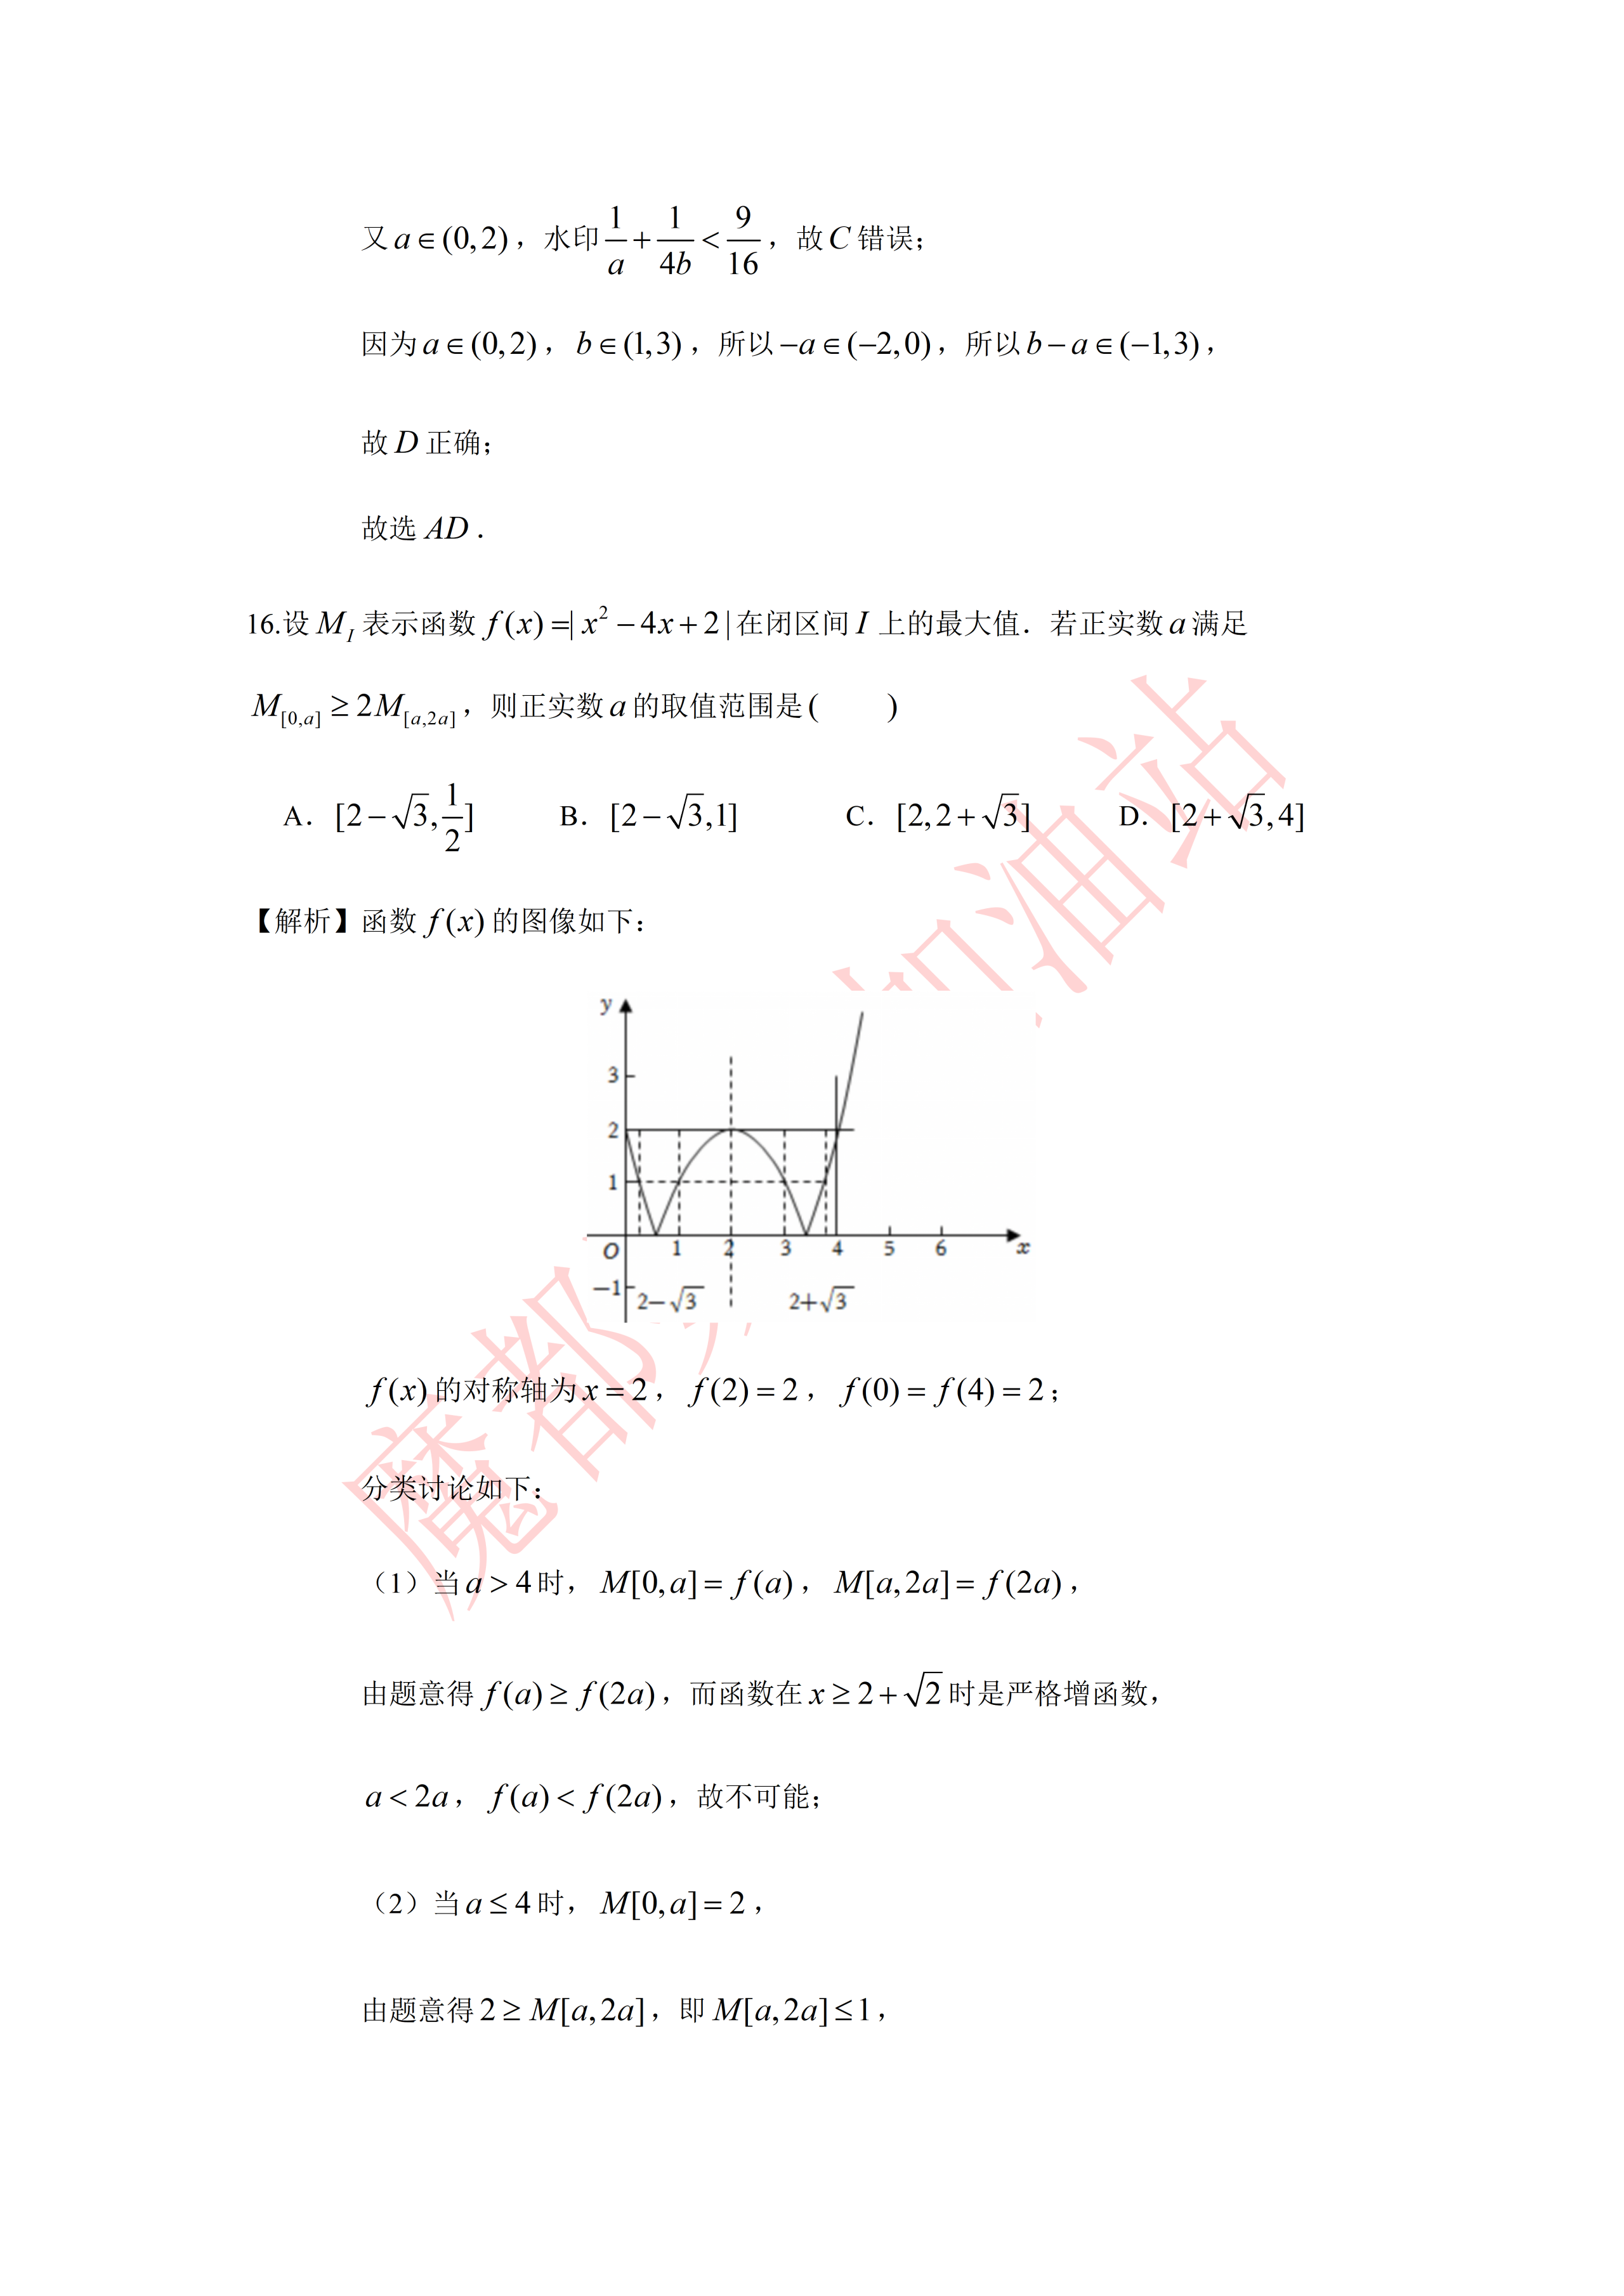
\includegraphics[width=.55\linewidth,trim=895bp 1535bp 915bp 1525bp,clip]{../原图/高一51_华师大二附中_国庆作业3/06.png}
\end{center}
\step{$f(x)$ 的对称轴为 $x=2$，$f(2)=2$，$f(0)=f(4)=2$；}
\step{分类讨论如下：}
\stepm{(1)}{当 $a>4$ 时，$M_{[0,a]}=f(a)$，$M_{[a,2a]}=f(2a)$，}
\step{由题意得 $f(a)\geqslant f(2a)$，而函数在 $x\geqslant2+\sqrt2$ 时是严格增函数，}
\step{$a<2a$，$f(a)<f(2a)$，故不可能；}
\stepm{(2)}{当 $a\leqslant4$ 时，$M_{[0,a]}=2$，}
\step{由题意得 $2\geqslant M_{[a,2a]}$，即 $M_{[a,2a]}\leqslant1$，}
\step{令 $f(x)=1$，解得 $x_1=2-\sqrt3$，$x_2=1$，$x_3=2+\sqrt3$，$x_4=3$，}
\step{则有 $a\geqslant2-\sqrt3$ 并且 $2a\leqslant1$，解得 $2-\sqrt3\leqslant a\leqslant\dfrac12$；}
\step{或者 $a\geqslant3$ 并且 $2a\leqslant2+\sqrt3$，无解；}
\step{故选 $A$.}
\solend

\fi

\end{enumerate}

\bigsec{三、解答题}

\begin{enumerate}
\setcounter{enumi}{16}

\item 已知 $M=\{x\mid2\leqslant x\leqslant5\}$，$N=\{x\mid a-1\leqslant x\leqslant2a+1\}$.
\begin{enumerate}[label=(\arabic*)]
\item 若 $M\subseteq N$，求实数 $a$ 的取值范围；
\item 若 $M\supseteq N$，求实数 $a$ 的取值范围.
\end{enumerate}

\ifanswer
\ans{（1）$[2,3]$；（2）$(-\infty,-2)$}
\fi

\ansspace[6]

\item 设集合 $A=\{x\mid|x+1|\leqslant3\}$，$B=\{x\mid0<x<3m\}$.
\begin{enumerate}[label=(\arabic*)]
\item 若 $A\cup B=A$，求实数 $m$ 的取值范围；
\item 设 $P=(\complement_R A)\cap B$，若 $\exists x\in\Z$ 且 $x\in P$，求实数 $m$ 的取值范围.
\end{enumerate}

\ifanswer
\solbegin
\stepm{(1)}{$A=\{x\mid|x+1|\leqslant3\}=\{x\mid-4\leqslant x\leqslant2\}$，且 $A\cup B=A$，所以 $B\subseteq A$.}
\step{若 $B=\varnothing$，此时 $0\geqslant3m$，解得 $m\leqslant0$；}
\step{若 $B\neq\varnothing$，此时 $0<3m$，且 $3m\leqslant2$，解得 $0<m\leqslant\dfrac23$；}
\step{则实数 $m$ 的取值范围是 $\left(-\infty,\dfrac23\right]$.}
\stepm{(2)}{因为 $\exists x\in\Z$ 且 $x\in P$，所以集合 $P$ 中至少存在一个整数.}
\step{$\complement_R A=\{x\mid x<-4\text{ 或 }x>2\}$，$B=\{x\mid0<x<3m\}$，}
\step{要使 $P=(\complement_R A)\cap B$ 中至少存在一个整数，则 $\begin{cases}3m>0\\3m>3\end{cases}$，解得 $m>1$，}
\step{则实数 $m$ 的取值范围是 $(1,+\infty)$.}
\solend

\fi

\ansspace[7]

\item 已知函数 $f(x)=x^2+(1-a)x-a(a\in\R)$.
\begin{enumerate}[label=(\arabic*)]
\item 解关于 $x$ 的不等式 $f(x)<0$；
\item 若 $\forall a\in[-1,1]$，$f(x)\geqslant0$ 恒成立，求实数 $x$ 的取值范围.
\end{enumerate}

\ifanswer
\solbegin
\stepm{(1)}{不等式 $x^2+(1-a)x-a<0$ 等价于 $(x-a)(x+1)<0$，}
\step{当 $a<-1$ 时，不等式的解集为 $(a,-1)$；}
\step{当 $a=-1$ 时，不等式的解集为 $\varnothing$；}
\step{当 $a>-1$ 时，不等式的解集为 $(-1,a)$.}
\stepm{(2)}{$x^2+(1-a)x-a=-a(x+1)+x^2+x$，}
\step{设 $g(a)=-a(x+1)+x^2+x$，$a\in[-1,1]$，}
\step{要使 $g(a)\geqslant0$ 在 $a\in[-1,1]$ 上恒成立，}
\step{只需 $\begin{cases}g(-1)\geqslant0\\g(1)\geqslant0\end{cases}$，即 $\begin{cases}x^2+2x+1\geqslant0\\x^2-1\geqslant0\end{cases}$，解得 $x\geqslant1$ 或 $x\leqslant-1$，}
\step{所以 $x$ 的取值范围为 $\{x\mid x\leqslant-1\text{ 或 }x\geqslant1\}$.}
\solend

\fi

\ansspace[7]

\item 若实数 $x$、$y$、$m$ 满足 $|x-m|>|y-m|$，则称 $x$ 比 $y$ 远离 $m$.
\begin{enumerate}[label=(\arabic*)]
\item 若 $2$ 比 $3x-4$ 远离 $1$，求 $x$ 的取值范围；
\item 设 $y=\dfrac{x+2}{x+1}$，其中 $x\in(0,\sqrt2)\cup(\sqrt2,+\infty)$，判断：$x$ 与 $y$ 哪一个更远离 $\sqrt2$？并说明理由.
\item 若 $x+y=2$，试问：$y$ 与 $x^2+y^2$ 哪一个更远离 $\dfrac12$？并说明理由.
\end{enumerate}

\ifanswer
\solbegin
\stepm{(1)}{由题意得 $|2-1|>|3x-4-1|$，所以 $|3x-5|<1$，解得 $\dfrac43<x<2$，}
\step{故 $x$ 的取值范围为 $\left(\dfrac43,2\right)$；}
\stepm{(2)}{$x$ 比 $y$ 更远离 $\sqrt2$，}
\step{理由如下：要证 $x$ 比 $y$ 更远离 $\sqrt2$，只要证 $|x-\sqrt2|>\left|\dfrac{x+2}{x+1}-\sqrt2\right|$，}
\step{即证 $|x-\sqrt2|>\left|\dfrac{(1-\sqrt2)(x-\sqrt2)}{x+1}\right|$，}
\step{因为 $x\in(0,\sqrt2)\cup(\sqrt2,+\infty)$，所以 $|x-\sqrt2|>0$，}
\step{所以只要证 $1>\dfrac{\sqrt2-1}{|x+1|}$，即证 $|x+1|>\sqrt2-1$，}
\step{因为 $x\in(0,\sqrt2)\cup(\sqrt2,+\infty)$，所以 $x+1\in(1,\sqrt2+1)\cup(\sqrt2+1,+\infty)$，}
\step{所以 $|x+1|>1>\sqrt2-1$，所以 $x$ 比 $y$ 更远离 $\sqrt2$；}
\stepm{(3)}{因为 $x^2+y^2\geqslant\dfrac{(x+y)^2}{2}=2$，当且仅当 $x=y=1$ 时等号成立，}
\step{所以 $\left|x^2+y^2-\dfrac12\right|=x^2+y^2-\dfrac12$，}
\step{从而 $\left|y-\dfrac12\right|-\left|x^2+y^2-\dfrac12\right|=\left|y-\dfrac12\right|-\left(x^2+y^2-\dfrac12\right)$，}
\step{①$y\geqslant\dfrac12$，$\left|y-\dfrac12\right|-\left|x^2+y^2-\dfrac12\right|=y-\dfrac12-\left(x^2+y^2-\dfrac12\right)=y-x^2-y^2$}
\step{$=y-(2-y)^2-y^2=-2y^2+5y-4=-2\left(y-\dfrac54\right)^2-\dfrac78<0$，}
\step{即 $\left|y-\dfrac12\right|<\left|x^2+y^2-\dfrac12\right|$；}
\step{②$y<\dfrac12$，}
\step{$\left|y-\dfrac12\right|-\left|x^2+y^2-\dfrac12\right|=\left(\dfrac12-y\right)-\left(x^2+y^2-\dfrac12\right)=-y-x^2-y^2+1$}
\step{$=-y-(2-y)^2-y^2+1=-2y^2+3y-3=-2\left(y-\dfrac34\right)^2-\dfrac{15}8<0$，}
\step{即 $\left|y-\dfrac12\right|<\left|x^2+y^2-\dfrac12\right|$；}
\step{综上，$\left|y-\dfrac12\right|<\left|x^2+y^2-\dfrac12\right|$，即 $x^2+y^2$ 比 $y$ 更远离 $\dfrac12$.}
\solend

\fi

\ansspace[9]

\item 对于非空有限整数集 $X$，$m\in\N^*$，定义 $X^m=\{x^m\mid x\in X\}$，对 $n\in\Z$，
$Y\oplus n=\{x+n\mid x\in Y\}$ 现有两个非空有限整数集 $A$、$B$，已知 $A\oplus1\subseteq B$ 且
$B^2\oplus(-4)\subseteq A$.
\begin{enumerate}[label=(\arabic*)]
\item 当 $A=\{-3,0\}$ 时求集合 $B$；
\item 证明：$A\subseteq\{-3,-2,0,1\}$；
\item 当 $A\oplus1=B$ 且 $B^2\oplus(-4)=A$ 时，任取 $a\in A$，$b\in B$ 构造函数
$f(x)=(x-a)(x-b)$ 问：当 $a$、$b$ 取何值时，$f(x)$ 的最小值最小？
\end{enumerate}

\ifanswer
\solbegin
\stepm{(1)}{因为 $A=\{-3,0\}$，$B^2\oplus(-4)\subseteq A$，}
\step{所以 $B^2\oplus(-4)$ 可能为 $\varnothing$、$\{-3\}$、$\{0\}$、$\{-3,0\}$，}
\step{当 $B^2\oplus(-4)=\varnothing$ 时 $B^2=\varnothing$，不满足非空，不合题意；}
\step{当 $B^2\oplus(-4)=\{-3\}$ 时 $B^2=\{1\}$，所以 $B=\{1,-1\}$、$\{1\}$、$\{-1\}$，}
\step{当 $B^2\oplus(-4)=\{0\}$ 时 $B^2=\{4\}$，所以 $B=\{2,-2\}$、$\{2\}$、$\{-2\}$，}
% 原卷如此，照录未改（此处作 $\{0,-3\}$，上一行同一集合作 $\{-3,0\}$）
\step{当 $B^2\oplus(-4)=\{0,-3\}$ 时 $B^2=\{4,1\}$，}
\step{所以 $B=\{1,2,-1,-2\}$、$\{2,-1,-2\}$、$\{2,1,-2\}$、$\{1,-1,-2\}$、$\{1,-1,2\}$、$\{1,2\}$、$\{-1,2\}$、$\{-1,-2\}$、$\{1,-2\}$，}
\step{又 $A\oplus1=\{-2,1\}\subseteq B$，得 $B$ 为 $\{1,-2\}$、$\{2,1,-2\}$、$\{1,-1,-2\}$、$\{1,2,-1,-2\}$.}
\stepm{(2)}{设 $x\in A$，因为 $A\oplus1\subseteq B$，所以 $x+1\in B$，}
\step{又 $B^2\oplus(-4)\subseteq A$，所以 $(x+1)^2-4\in A$，}
% 原卷如此，照录未改（此处及下文取 $x=2$ 处原卷均作 $(-4+1)^2-4=52-2a>0$）
\step{取 $x=-4$，则 $(-4+1)^2-4=52-2a>0$，$(5+1)^2-4=32\in A$，$\cdots$，}
\step{无限迭代，而 $A$ 为有限集，不合题意，舍去，即 $-4\notin A$；}
\step{取 $x=-3$，则 $(-3+1)^2-4=0\in A$，$(0+1)^2-4=-3\in A$，}
\step{得 $A$ 集合可为 $\{-3,0\}$；}
\step{取 $x=-2$，则 $(-2+1)^2-4=-3\in A$，$(-3+1)^2-4=0\in A$，}
\step{$(0+1)^2-4=-3\in A$，得 $A$ 集合可为 $\{-3,-2,0\}$；}
\step{取 $x=-1$，则 $(-1+1)^2-4=-4\in A$，又 $-4\notin A$，所以 $-1\notin A$，}
\step{取 $x=1$，则 $(1+1)^2-4=0\in A$，$(0+1)^2-4=-3\in A$，}
\step{$(-3+1)^2-4=0\in A$，得 $A$ 集合可为 $\{-3,0,1\}$，}
\step{取 $x=2$，则 $(2+1)^2-4=52-2a>0$，$(5+1)^2-4=32\in A$，$\cdots$，}
\step{无限迭代，而 $A$ 为有限集，不合题意，舍去，即 $2\notin A$，}
\step{同理当 $x<-4$ 或 $x>2$，且 $x\in\Z$ 时不符合 $A$ 为有限集，舍去；}
\step{故由上得 $A$ 集合可为 $\{-3,0\},\{-3,-2,0\},\{-3,0,1\},\{-3,-2,0,1\}$，}
\step{所以 $A\subseteq\{-3,-2,0,1\}$，}
\stepm{(3)}{当 $A\oplus1=B$ 且 $B^2\oplus(-4)=A$ 时，}
\step{设 $x\in B$，则 $x^2-4\in B^2\oplus(-4)=A$，}
% 原卷如此，照录未改（题设 $A=\{-3,0\}$，此处两个判别式取的是 $-2$ 与 $1$，均不属于 $A$）
\step{$x^2-4=-2$ 时 $x=\pm\sqrt2$，不为整数，不合题意；}
\step{$x^2-4=1$ 时 $x=\pm\sqrt5$，不为整数，不合题意；}
\step{所以 $A=\{-3,0\}$，又 $A\oplus1=B$，则 $B=\{-2,1\}$，}
\step{任取 $a\in A$，$b\in B$ 构造函数 $f(x)=(x-a)(x-b)$，}
\step{$f(x)=(x-a)(x-b)=x^2-(a+b)x+ab$}
\step{$=x^2-(a+b)x+\dfrac{(a+b)^2}{4}+ab-\dfrac{(a+b)^2}{4}$}
\step{$=\left[x-\dfrac{(a+b)}2\right]^2-\dfrac{(a-b)^2}{4}\geqslant-\dfrac{(a-b)^2}{4}$，所以 $f(x)_{min}=-\dfrac{(a-b)^2}{4}$，}
\step{又 $a\in A=\{-3,0\}$，$b\in B=\{-2,1\}$，所以 $a-b$ 的取值有 $-1,-4,2$，}
\step{所以 $f(x)_{min}=-\dfrac{(a-b)^2}{4}\geqslant-\dfrac{(-3-1)^2}{4}=-4$，}
\step{即当 $a=-3$，$b=1$ 时 $f(x)_{min}$ 的最小值为 $-4$.}
\solend

\fi

\ansspace*[12]

\end{enumerate}

\end{document}
"
%
% 原始材料：微信公众号“魔都数学加油站”文章，作者破晓，连载“27学年高一51”；
% 原文标题“27学年高一51——2026-2027年上海市华师大二附中高一上国庆作业3”；
% 原文链接：https://mp.weixin.qq.com/s/95SLMEmPUT30s4U7wjr5Og。
% 该页面用 JS 渲染，未见明确发布日期；页面内时间戳约为 2026-10-05 21:37，本稿以该时刻记可得日期。
% 正文为 12 张 PNG 页：第 01、02、03、05、07、08、11 页 4762×6735，
% 第 04、06、09、10、12 页 2560×3620。按页序逐页读取，12 页全为试卷正文页
% （卷首标题在第 1 页页顶，卷末解答题止于第 12 页），无封面页、目录页或单独的页脚页。
% 卷面标题照原卷印作“2026-2027 年华师大二附中高一上国庆作业 3”（公众号标题中的“上海市”
% 卷面标题行没有，本稿照卷面），年份区间按全稿惯例排 en dash。
%
% 篇幅与题号：原卷自第 3 题起编号（第 1、2 题不在本卷内）。填空题 3—12（10 题）、
% 选择题 13—16（4 题）、解答题 17—21（5 题），共 19 题。本稿沿用原节与原题号，
% 只改排为全稿统一的大节样式（原卷小节标题为“一、填空题”“二、选择题”“三、解答题”）。
% 正文为讲评版：填空题 3—12 与选择题 13—16 只印【解析】（选择题的结论“故选 X”印在解析内），
% 按全稿口径这类题不另提 \ans{}；解答题第 17 题只印【答案】，故只给 \ans{}；
% 第 18—21 题只印【解析】。
%
% 副标题：原卷未印副标题。本稿按“知识模块”口径标作“集合与常用逻辑用语、不等式”：
% 19 题中集合与常用逻辑用语 8 题（3、4、6、10、13、17、18、21），
% 不等式（含函数最值、绝对值不等式）11 题（5、7、8、9、11、12、14、15、16、19、20），
% 两类均远超三分之一，故并标。口径同 高一46_交附闵行_国庆作业3、高一48_华师大二附中_周末作业2。
%
% 与原卷的排版差异：
%   ① 原卷每题下直接印【答案】或【解析】，本稿按全稿惯例将答案与解析置于答案版；
%   ② 原卷未印副标题，本稿按“知识模块”口径补出；
%   ③ 原卷填空横线按全稿惯例排为 \blankline[4.4em]；
%   ④ 原卷 $R$、$N$、$Z$ 均排斜体，本稿按全稿惯例改用花体 $\R$、$\N$、$\Z$（同 高一48）；
%   ⑤ 原卷第 12 题解析配图、第 13 题题干韦恩图都印在正文右侧的浮动位置，第 16 题解析配图
%      印在解析行间；本稿三图一律居中排，均自原图对应页裁切（trim），不另存图片文件；
%   ⑥ 原卷解答题未留作答空白，本稿按全稿惯例加 \ansspace；
%   ⑦ 原卷第 15 题解析第 7、8 两个印刷行是一串连等式的折行，本稿按“一条 \step ＝ 一个印刷行”
%      的口径分成两条 \step。
%
% 原卷笔误/存疑（均照录未改，正文对应处另有 % 注）：
%   ① 第 12 题解析末行作“区间长度之和为 $x_1-b+x_2-a=x_1-x_2-a-b=2+a+b-a-b=2$”，
%      按上一行 $x_1+x_2=2+a+b$，此处应为 $x_1+x_2$；原卷作 $x_1-x_2$。
%   ② 第 15 题解析“又 $a\in(0,2)$，”与 $\dfrac1a+\dfrac1{4b}<\dfrac9{16}$ 之间，
%      原卷正文夹印“水印”二字（系制版遗留字样，非试卷内容）。
%   ③ 第 21 题第 (2) 问解析两处（取 $x=-4$、取 $x=2$）作“$=52-2a>0$”，
%      与题设 $(x+1)^2-4$ 的取值（按 $x=-4$ 应为 $5$）不符，当系原卷算式遗留。
%   ④ 第 21 题第 (1) 问解析先写 $B^2\oplus(-4)$ 可能为 $\{-3,0\}$，后文又作 $\{0,-3\}$，
%      同一集合两种写法。
%   ⑤ 第 21 题第 (3) 问解析：题设 $B^2\oplus(-4)=A$ 且 $A=\{-3,0\}$ 时，由 $x^2-4\in A$
%      应得 $x^2-4=-3$ 或 $0$；原卷讨论的却是 $x^2-4=-2$ 与 $x^2-4=1$（两值均不属于 $A$），
%      与题设不合。
%
% 插图：3 张，均自原图裁切（无 \begin{tikzpicture} 重排）：
%   · 第 13 题题干韦恩图（原图第 04 页，图在题干与选项右侧）
%   · 第 12 题解析配图（原图第 04 页，图在解析右侧）
%   · 第 16 题解析配图（原图第 06 页，图在解析中间）
%
\documentclass[a4paper,11pt]{article}
\usepackage{common}

\begin{document}

\examtitlest[3]{2026--2027 年华师大二附中高一上国庆作业 3}{集合与常用逻辑用语、不等式}

\bigsec{一、填空题}

\begin{enumerate}
\setcounter{enumi}{2}

\item 若 $\{x\mid x<1\text{ 或 }x>4\}\cup\{x\mid m<x<2m+3\}=R$，则实数 $m$ 的取值范围为\blankline[4.4em].

\ifanswer
\solbegin
\step{因为 $\{x\mid x<1\text{ 或 }x>4\}\cup\{x\mid m<x<2m+3\}=R$，}
\step{所以 $\begin{cases}m<1\\2m+3>4\end{cases}$，解得 $\dfrac12<m<1$，所以 $m$ 的取值范围为 $\left(\dfrac12,1\right)$.}
\solend

\fi

\item 若“$x\leqslant5$”是“$x<a$”的必要不充分条件，则 $a$ 的取值范围是\blankline[4.4em].

\ifanswer
\solbegin
\step{若“$x\leqslant5$”是“$x<a$”的必要不充分条件，则 $\{x\mid x<a\}\subset\{x\mid x\leqslant5\}$，}
\step{所以 $a\leqslant5$.}
\solend

\fi

\item 实数 $x$、$y$ 满足 $x^2+2xy+4y^2=1$，则 $x+2y$ 的取值范围是\blankline[4.4em].

\ifanswer
\solbegin
\step{因为 $x^2+2xy+4y^2=(x+2y)^2-2xy=1$，}
\step{所以 $(x+2y)^2-1=x\cdot(2y)\leqslant\left(\dfrac{x+2y}{2}\right)^2$，当且仅当 $x=2y$ 时取等号，}
\step{解得 $-\dfrac{2\sqrt3}{3}\leqslant x+2y\leqslant\dfrac{2\sqrt3}{3}$，故 $x+2y$ 的取值范围是 $\left[-\dfrac{2\sqrt3}{3},\dfrac{2\sqrt3}{3}\right]$.}
\solend

\fi

\item 若命题 $p$：“$\exists x\in\R$，$5x^2-3x+m=0$”为假命题，则实数 $m$ 的取值范围为\blankline[4.4em].

\ifanswer
\solbegin
\step{若命题 $p$：$\exists x\in\R$，$5x^2-3x+m=0$ 为假命题，}
\step{则 $5x^2-3x+m=0$ 没有实数根，故 $\Delta=9-20m<0$，解得 $m>\dfrac9{20}$.}
\solend

\fi

\item 若当 $3\leqslant m\leqslant5$ 时，$mx^2-mx+m-9<0$ 有解，则实数 $x$ 的取值范围是\blankline[4.4em].

\ifanswer
\solbegin
\step{当 $3\leqslant m\leqslant5$ 时，$mx^2-mx+m-9<0$ 有解，}
\step{即 $(x^2-x+1)m-9<0$ 在 $m\in[3,5]$ 上有解，}
\step{因为 $x^2-x+1>0$，所以一次函数 $g(m)=(x^2-x+1)m-9$ 严格增，}
\step{所以只需 $g(3)=3x^2-3x-6<0$ 即可，}
\step{即 $x^2-x-2<0$，$(x-2)(x+1)<0$，解得 $-1<x<2$，}
\step{所以实数 $x$ 的取值范围是 $(-1,2)$.}
\solend

\fi

\item 已知不等式 $\dfrac{x}{x^2+4}\leqslant a$ 对任意的 $x\in[1,3]$ 恒成立，则实数 $a$ 的范围为\blankline[4.4em].

\ifanswer
\solbegin
\step{因为 $x\in[1,3]$，所以 $\dfrac{x}{x^2+4}=\dfrac{1}{x+\dfrac4x}\leqslant\dfrac{1}{2\sqrt{x\times\dfrac4x}}=\dfrac14$，}
\step{当且仅当 $x=\dfrac4x$ 时，即 $x=2$ 时取等号，即 $\dfrac{x}{x^2+4}$ 在 $x\in[1,3]$ 的最大值为 $\dfrac14$，}
\step{又由不等式 $\dfrac{x}{x^2+4}\leqslant a$ 对任意的 $x\in[1,3]$ 恒成立，所以 $a\geqslant\dfrac14$，}
\step{即实数 $a$ 的范围为 $\left[\dfrac14,+\infty\right)$.}
\solend

\fi

\item 甲、乙两人解关于 $x$ 的不等式 $x^2+bx+c<0$，甲写错了 $b$，正确计算后得到的解为 $\{x\mid1<x<2\}$；
乙写错了 $c$，正确计算后得到的解为 $\{x\mid-4<x<1\}$. 那么不等式 $\dfrac{bx+c}{x-2}<0$ 的解为\blankline[4.4em].

\ifanswer
\solbegin
\step{由 $x^2+bx+c<0$ 的解为 $\{x\mid1<x<2\}$，}
\step{则 $1$ 和 $2$ 是方程 $x^2+bx+c=0$ 的两个根，}
\step{甲写错了 $b$，但 $c$ 是正确的，所以 $c=1\times2=2$；}
\step{由 $x^2+bx+c<0$ 的解为 $\{x\mid-4<x<1\}$，}
\step{则 $-4$ 和 $1$ 是方程 $x^2+bx+c=0$ 的两个根，}
\step{乙写错了 $c$，但 $b$ 是正确的，所以 $-b=-4+1=-3$，即 $b=3$.}
\step{由 $\dfrac{bx+c}{x-2}<0$，得 $\dfrac{3x+2}{x-2}<0$，即 $(3x+2)(x-2)<0$，解得 $-\dfrac23<x<2$.}
\step{不等式 $\dfrac{bx+c}{x-2}<0$ 的解为 $\left\{x\mid-\dfrac23<x<2\right\}$.}
\solend

\fi

\item 已知 $\dfrac{1}{x-2}\geqslant1$ 是 $|x-a|<2$ 的充分非必要条件，则实数 $a$ 的取值范围是\blankline[4.4em].

\ifanswer
\solbegin
\step{由 $\dfrac{1}{x-2}\geqslant1$ 得 $\dfrac{3-x}{x-2}\geqslant0$，解得 $2<x\leqslant3$，由 $|x-a|<2$ 得 $a-2<x<a+2$，}
\step{因为 $\dfrac{1}{x-2}\geqslant1$ 是 $|x-a|<2$ 的充分非必要条件，}
\step{所以 $\{x\mid2<x\leqslant3\}\subset\{x\mid a-2<x<a+2\}$，所以 $\begin{cases}a-2\leqslant2\\a+2>3\end{cases}$，解得 $1<a\leqslant4$，}
\step{即实数 $a$ 的取值范围是 $(1,4]$.}
\solend

\fi

\item 设 $a>0$，$b>0$，若不等式 $a(a+1)^2+b(b+1)^2\geqslant\lambda ab$ 恒成立，则实数 $\lambda$ 的最大值为\blankline[4.4em].

\ifanswer
\solbegin
\step{$a(a+1)^2+b(b+1)^2\geqslant\lambda ab\Leftrightarrow\lambda\leqslant\dfrac{a(a+1)^2+b(b+1)^2}{ab}=\dfrac{(a+1)^2}{b}+\dfrac{(b+1)^2}{a}$，}
\step{从而原问题转化为求 $\dfrac{(a+1)^2}{b}+\dfrac{(b+1)^2}{a}$ 的最小值.}
\step{因为 $\dfrac{(a+1)^2}{b}+\dfrac{(b+1)^2}{a}=\dfrac{b^2+2b+1}{a}+\dfrac{a^2+2a+1}{b}$}
\step{$=\left(\dfrac{b^2}{a}+\dfrac{a^2}{b}\right)+2\left(\dfrac ba+\dfrac ab\right)+\left(\dfrac1a+\dfrac1b\right)\geqslant2\sqrt{\dfrac{b^2}{a}\cdot\dfrac{a^2}{b}}+2\times2\sqrt{\dfrac ba\cdot\dfrac ab}+2\sqrt{\dfrac1a\cdot\dfrac1b}$}
\step{$=2\sqrt{ab}+4+\dfrac{2}{\sqrt{ab}}\geqslant2\sqrt{2\sqrt{ab}\cdot\dfrac{2}{\sqrt{ab}}}+4=8$，以上均当且仅当 $a=b$ 时取等号，}
\step{所以 $\lambda\leqslant8$，即实数 $\lambda$ 的最大值为 $8$.}
\solend

\fi

\item 定义区间 $(a,d)$、$[a,d)$、$(a,d]$、$[a,d]$ 的长度为 $d-a$（$d>a$），已知 $a>b$，则满足
$\dfrac{1}{x-a}+\dfrac{1}{x-b}\geqslant1$ 的 $x$ 构成的区间的长度之和为\blankline[4.4em].

\ifanswer
\solbegin
\step{因为 $\dfrac{1}{x-a}+\dfrac{1}{x-b}\geqslant1$，所以 $\dfrac{2x-(a+b)}{(x-a)(x-b)}\geqslant1$，}
\step{即 $\dfrac{2x-(a+b)}{(x-a)(x-b)}-1\geqslant0$，则 $\dfrac{x^2-(2+a+b)x+ab+a+b}{(x-a)(x-b)}\leqslant0$，}
\step{设 $x^2-(2+a+b)x+ab+a+b=0$ 的根为 $x_1$ 和 $x_2$，}
\begin{center}
% 原卷该图印在解析右侧（原图第 04 页），本稿移作居中排，直接裁取原图，不另存图片文件。
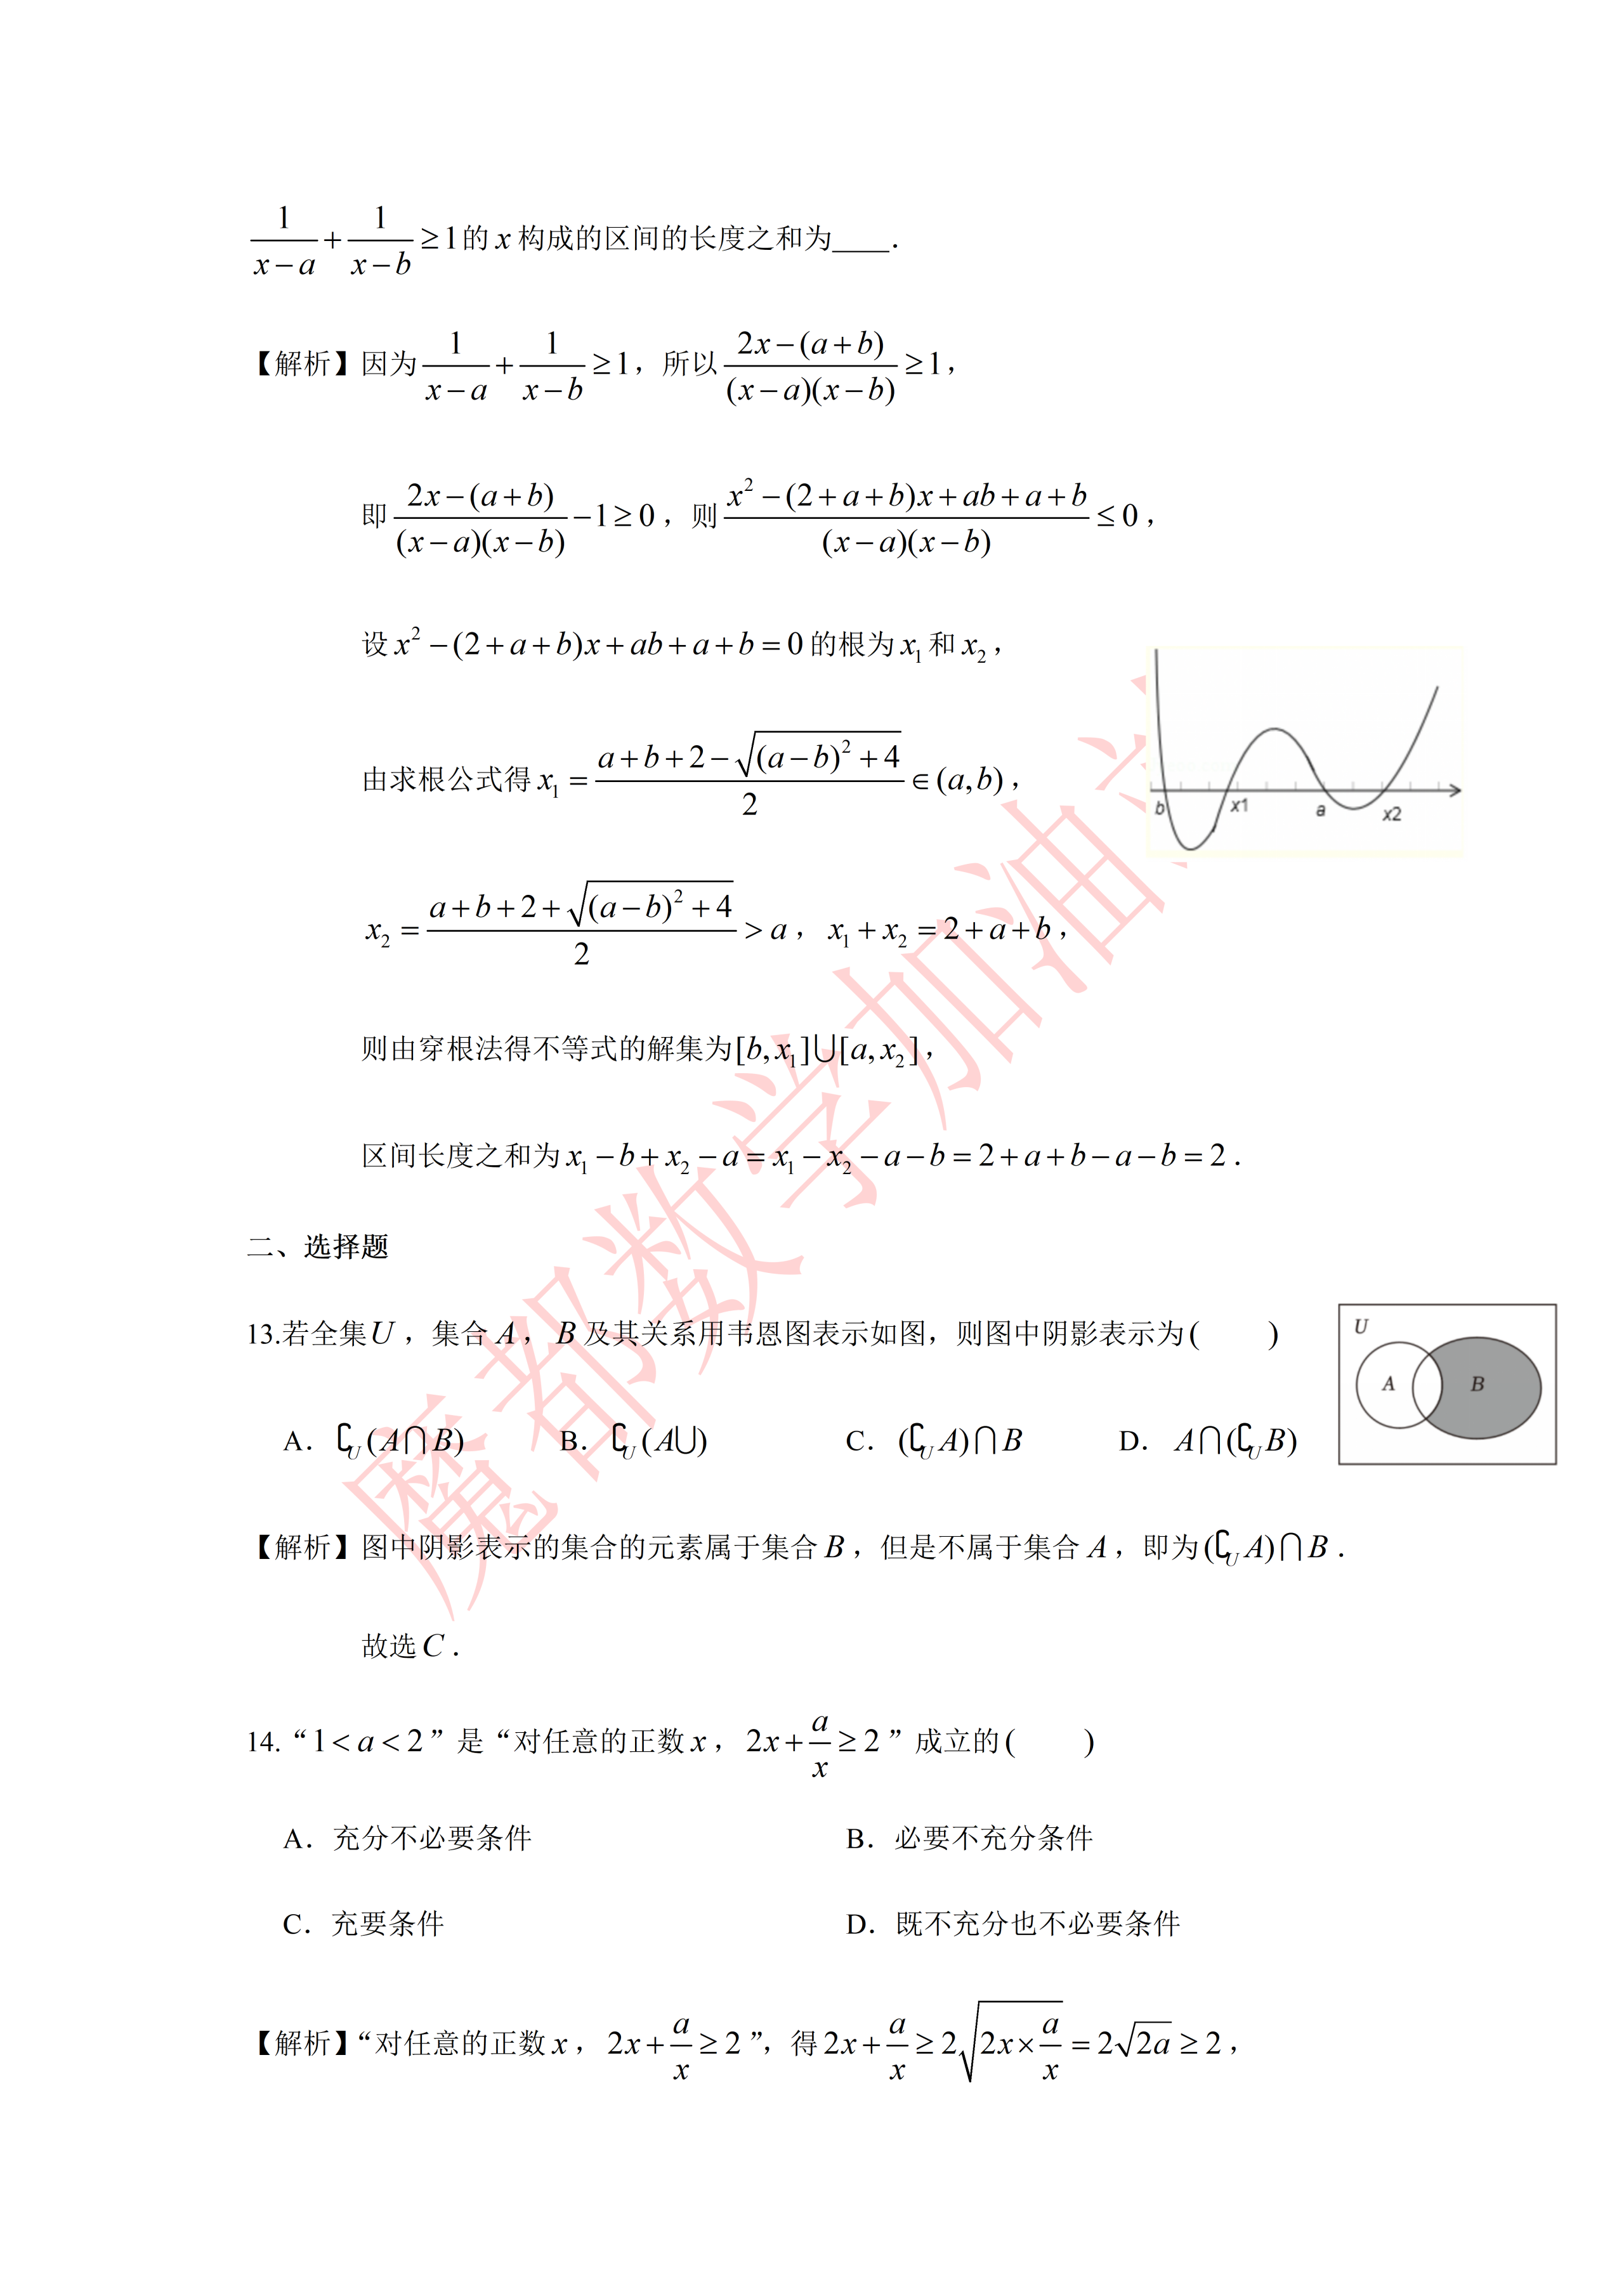
\includegraphics[width=.50\linewidth,trim=1786bp 2255bp 228bp 985bp,clip]{../原图/高一51_华师大二附中_国庆作业3/04.png}
\end{center}
\step{由求根公式得 $x_1=\dfrac{a+b+2-\sqrt{(a-b)^2+4}}{2}\in(a,b)$，}
\step{$x_2=\dfrac{a+b+2+\sqrt{(a-b)^2+4}}{2}>a$，$x_1+x_2=2+a+b$，}
\step{则由穿根法得不等式的解集为 $[b,x_1]\cup[a,x_2]$，}
% 原卷如此，照录未改（此处原卷作 $x_1-x_2$，按上一行 $x_1+x_2=2+a+b$ 当为 $x_1+x_2$）
\step{区间长度之和为 $x_1-b+x_2-a=x_1-x_2-a-b=2+a+b-a-b=2$.}
\solend

\fi

\end{enumerate}

\bigsec{二、选择题}

\begin{enumerate}
\setcounter{enumi}{12}

% 本题是“题干 + 图 + 选项”约 5.5cm 的一整块，图夹在题干与选项之间时 \keepwithprev 挡不住断点，
% 故按 高一30 第 13 题的成例在题前先量一次页高（守卫放在 \item 之前）。
\needvspace{6cm}
\item 若全集 $U$，集合 $A$、$B$ 及其关系用韦恩图表示如图，则图中阴影表示为\mbox{（\quad）}

\begin{center}
% 原卷该图印在题干与选项右侧（原图第 04 页），本稿移作居中排，直接裁取原图，不另存图片文件。
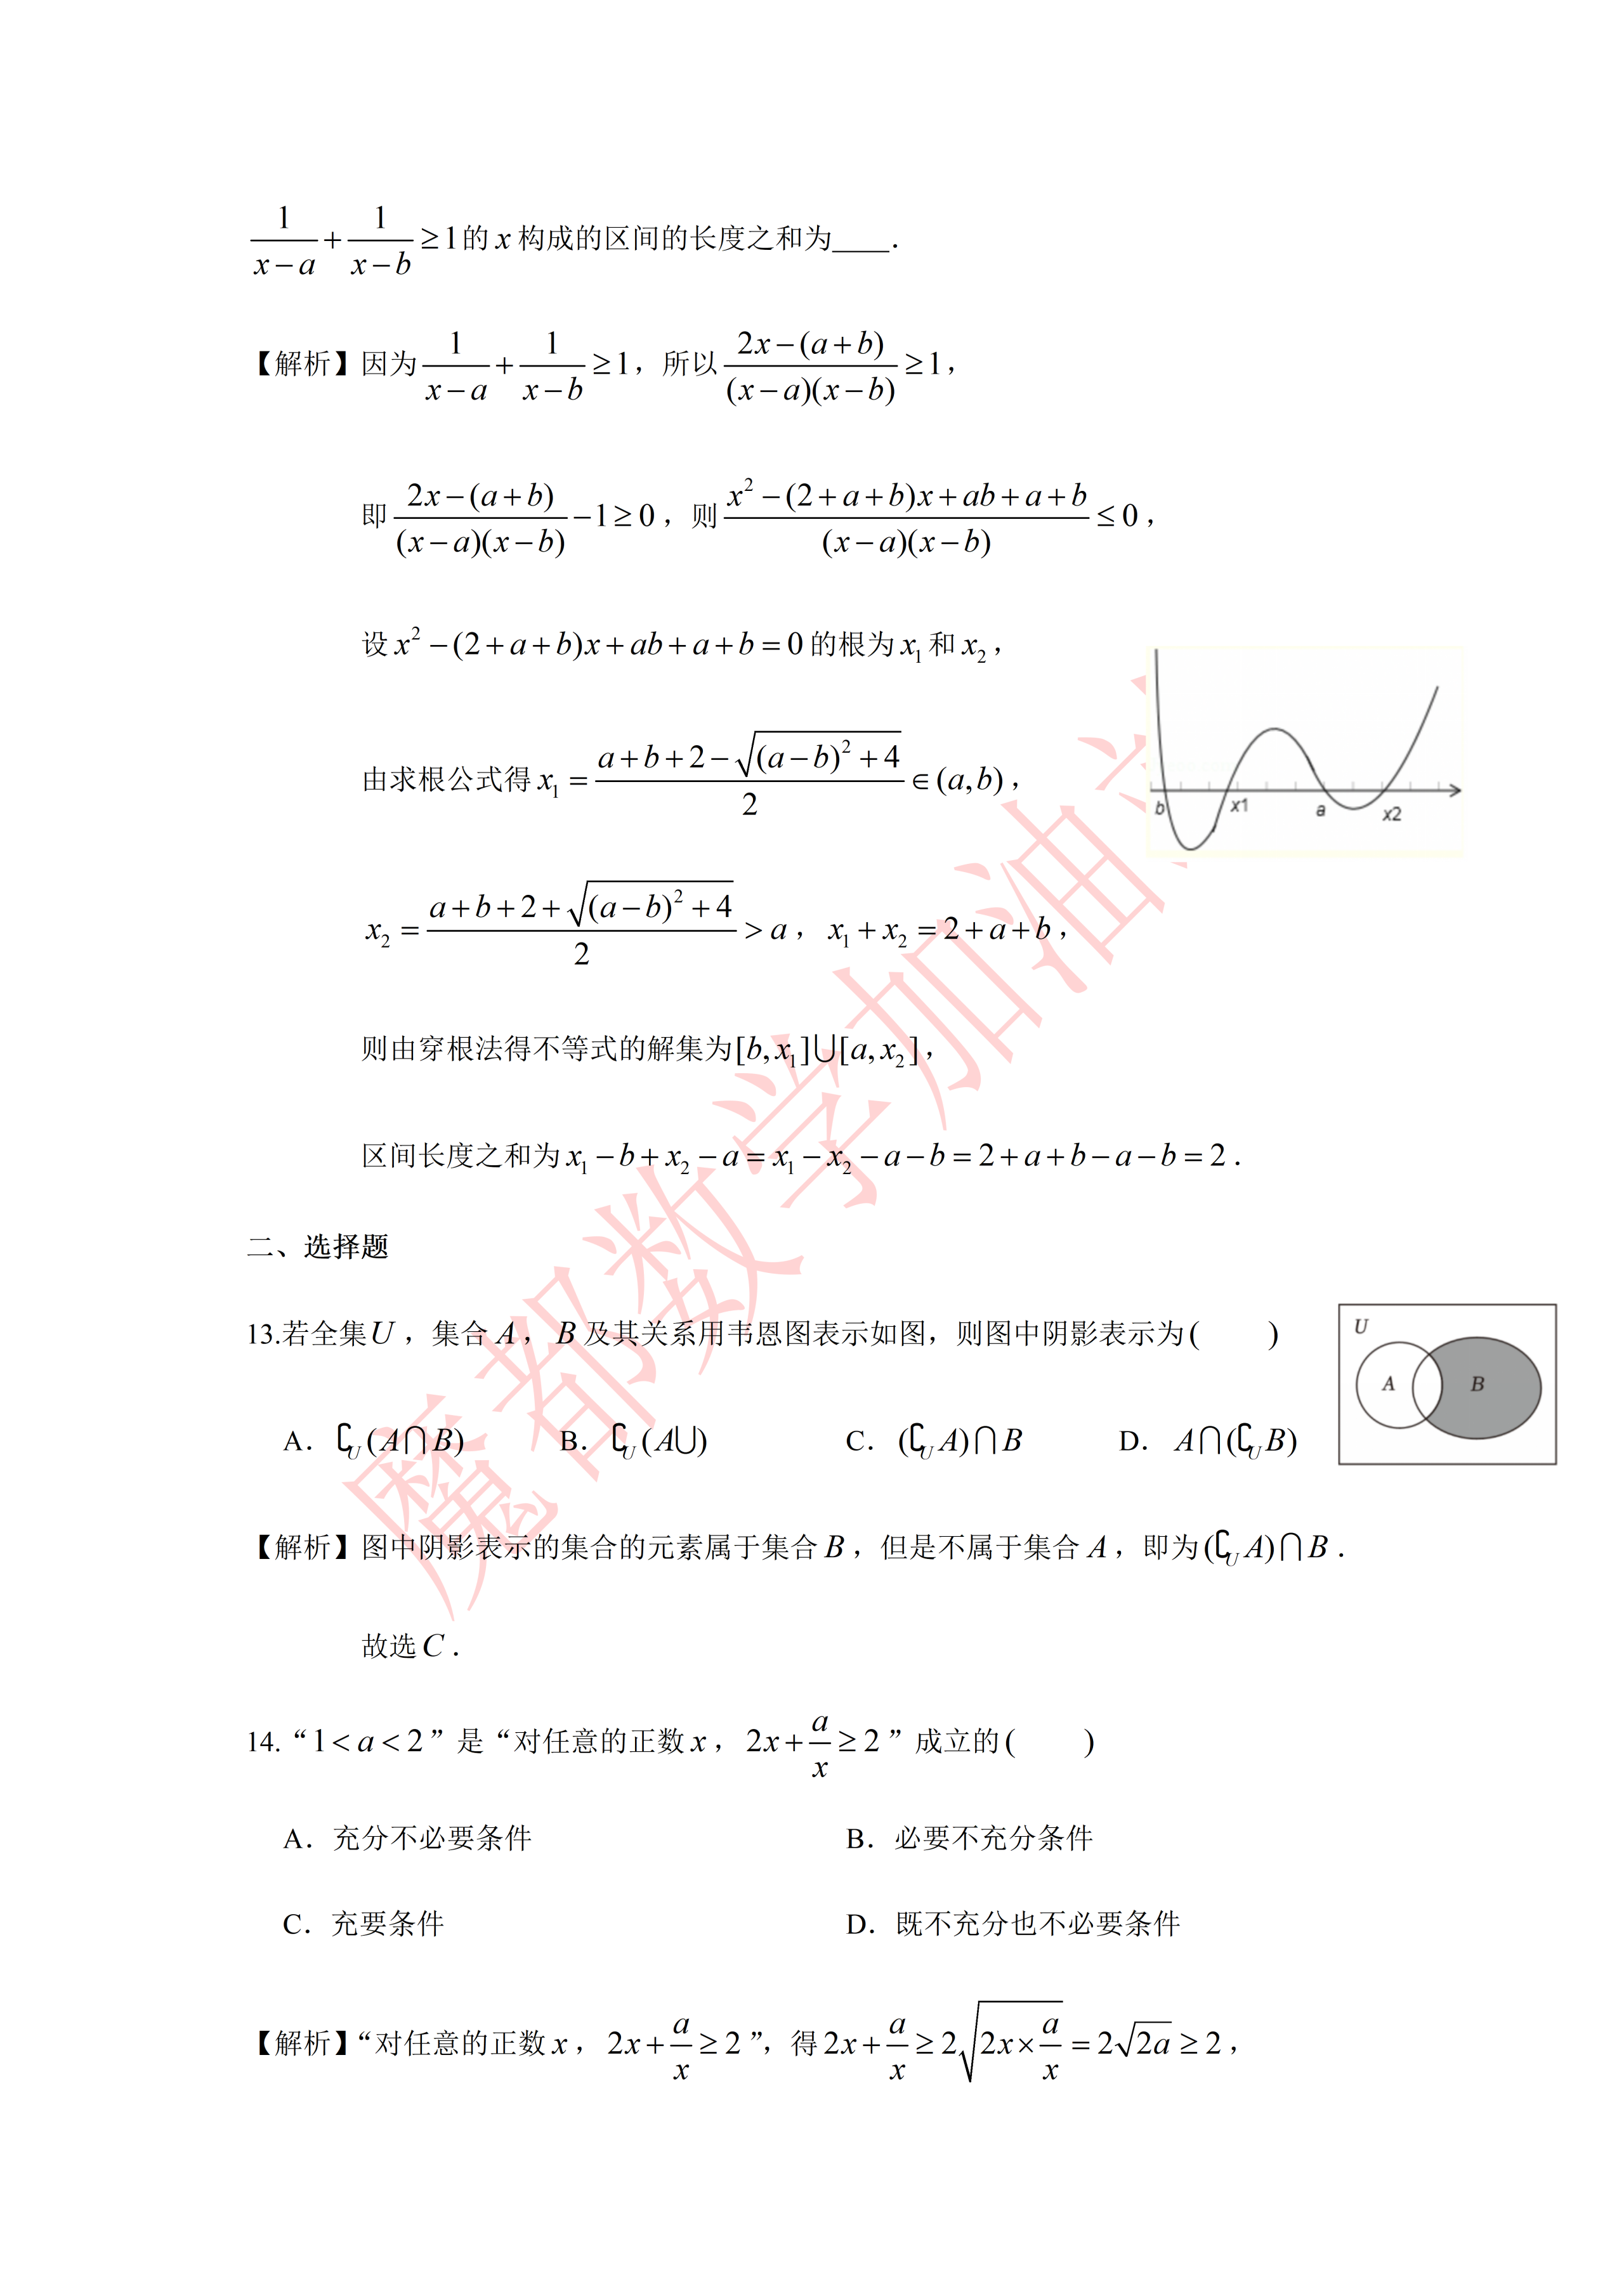
\includegraphics[width=.30\linewidth,trim=2105bp 1308bp 105bp 2050bp,clip]{../原图/高一51_华师大二附中_国庆作业3/04.png}
\end{center}

\keepwithprev
A. $\complement_U(A\cap B)$\qquad B. $\complement_U(A\cup B)$

C. $(\complement_U A)\cap B$\qquad D. $A\cap(\complement_U B)$

\ifanswer
\solbegin
\step{图中阴影表示的集合的元素属于集合 $B$，但是不属于集合 $A$，即为 $(\complement_U A)\cap B$.}
\step{故选 $C$.}
\solend

\fi

\item “$1<a<2$”是“对任意的正数 $x$，$2x+\dfrac ax\geqslant2$”成立的\mbox{（\quad）}

\keepwithprev
A. 充分不必要条件\qquad B. 必要不充分条件

C. 充要条件\qquad\qquad D. 既不充分也不必要条件

\ifanswer
\solbegin
\step{“对任意的正数 $x$，$2x+\dfrac ax\geqslant2$”，得 $2x+\dfrac ax\geqslant2\sqrt{2x\times\dfrac ax}=2\sqrt{2a}\geqslant2$，}
\step{所以 $\sqrt{2a}\geqslant1$，解得 $a\geqslant\dfrac12$，}
\step{若“$1<a<2$”得 $2x+\dfrac ax\geqslant2\sqrt{2x\times\dfrac ax}=2\sqrt{2a}>2\sqrt2>2$，}
\step{所以“$1<a<2$”$\Rightarrow$“对任意的正数 $x$，$2x+\dfrac ax\geqslant2$”，}
\step{所以“$1<a<2$”是“对任意的正数 $x$，$2x+\dfrac ax\geqslant2$”成立的充分不必要条件，}
\step{故选 $A$.}
\solend

\fi

\item 已知函数 $f(x)=2x-3$，$x\in(0,2)$，实数 $a$、$b$ 满足 $f(a)+f(b-1)=0$，则以下成立的有\mbox{（\quad）}

\keepwithprev
A. $a(b-1)$ 的最大值为 $\dfrac94$\qquad\qquad B. $b-\dfrac1a$ 的最大值为 $2$

C. $\dfrac1a+\dfrac1{4b}$ 的最小值为 $\dfrac9{16}$\qquad D. $-1<b-a<3$

\ifanswer
\solbegin
\step{因为函数 $f(x)=2x-3$，$x\in(0,2)$，实数 $a$、$b$ 满足 $f(a)+f(b-1)=0$，}
\step{所以 $2a-3+2(b-1)-3=0$，得 $a+b=4$，$a\in(0,2)$，$b\in(1,3)$，}
\step{所以 $a(b-1)=a(3-a)=-\left(a-\dfrac32\right)^2+\dfrac94$，$a\in(0,2)$，}
\step{所以 $0<a(b-1)\leqslant\dfrac94$，故选项 $A$ 正确；}
\step{$b-\dfrac1a=4-a-\dfrac1a=4-\left(a+\dfrac1a\right)\leqslant4-2=2$，}
\step{当且仅当 $a=1$，$b=3$ 时取等号，又 $b\in(1,3)$，故 $b-\dfrac1a<2$，故 $B$ 错误；}
\step{$\dfrac1a+\dfrac1{4b}=\dfrac14\left(\dfrac1a+\dfrac1{4b}\right)(a+b)=\dfrac14\left(1+\dfrac14+\dfrac ba+\dfrac a{4b}\right)=\dfrac5{16}+\dfrac14\left(\dfrac ba+\dfrac a{4b}\right)$}
\step{$\geqslant\dfrac5{16}+\dfrac14\cdot2\sqrt{\dfrac ba\cdot\dfrac a{4b}}=\dfrac9{16}$，当且仅当 $\dfrac ba=\dfrac a{4b}$，即 $a=2b=\dfrac83$ 时取等号，}
% 原卷如此，照录未改（“又 $a\in(0,2)$，”与下式之间原卷正文夹印“水印”二字）
\step{又 $a\in(0,2)$，水印 $\dfrac1a+\dfrac1{4b}<\dfrac9{16}$，故 $C$ 错误；}
\step{因为 $a\in(0,2)$，$b\in(1,3)$，所以 $-a\in(-2,0)$，所以 $b-a\in(-1,3)$，}
\step{故 $D$ 正确；}
\step{故选 $AD$.}
\solend

\fi

% 本题解析含图（“函数 f(x) 的图像如下”），图夹在解析行间，页末放不下会被拆开，
% 故在题前先量一次页高；上界取“题干 + 选项 + 图 + 首行解析”一块的高度。
\needvspace{6cm}
\item 设 $M_I$ 表示函数 $f(x)=|x^2-4x+2|$ 在闭区间 $I$ 上的最大值. 若正实数 $a$ 满足
$M_{[0,a]}\geqslant2M_{[a,2a]}$，则正实数 $a$ 的取值范围是\mbox{（\quad）}

\keepwithprev
A. $\left[2-\sqrt3,\dfrac12\right]$\qquad B. $[2-\sqrt3,1]$

C. $[2,2+\sqrt3]$\qquad\qquad D. $[2+\sqrt3,4]$

\ifanswer
\solbegin
\step{函数 $f(x)$ 的图像如下：}
\begin{center}
% 原卷该图印在解析行间（原图第 06 页），本稿直接裁取原图，不另存图片文件。
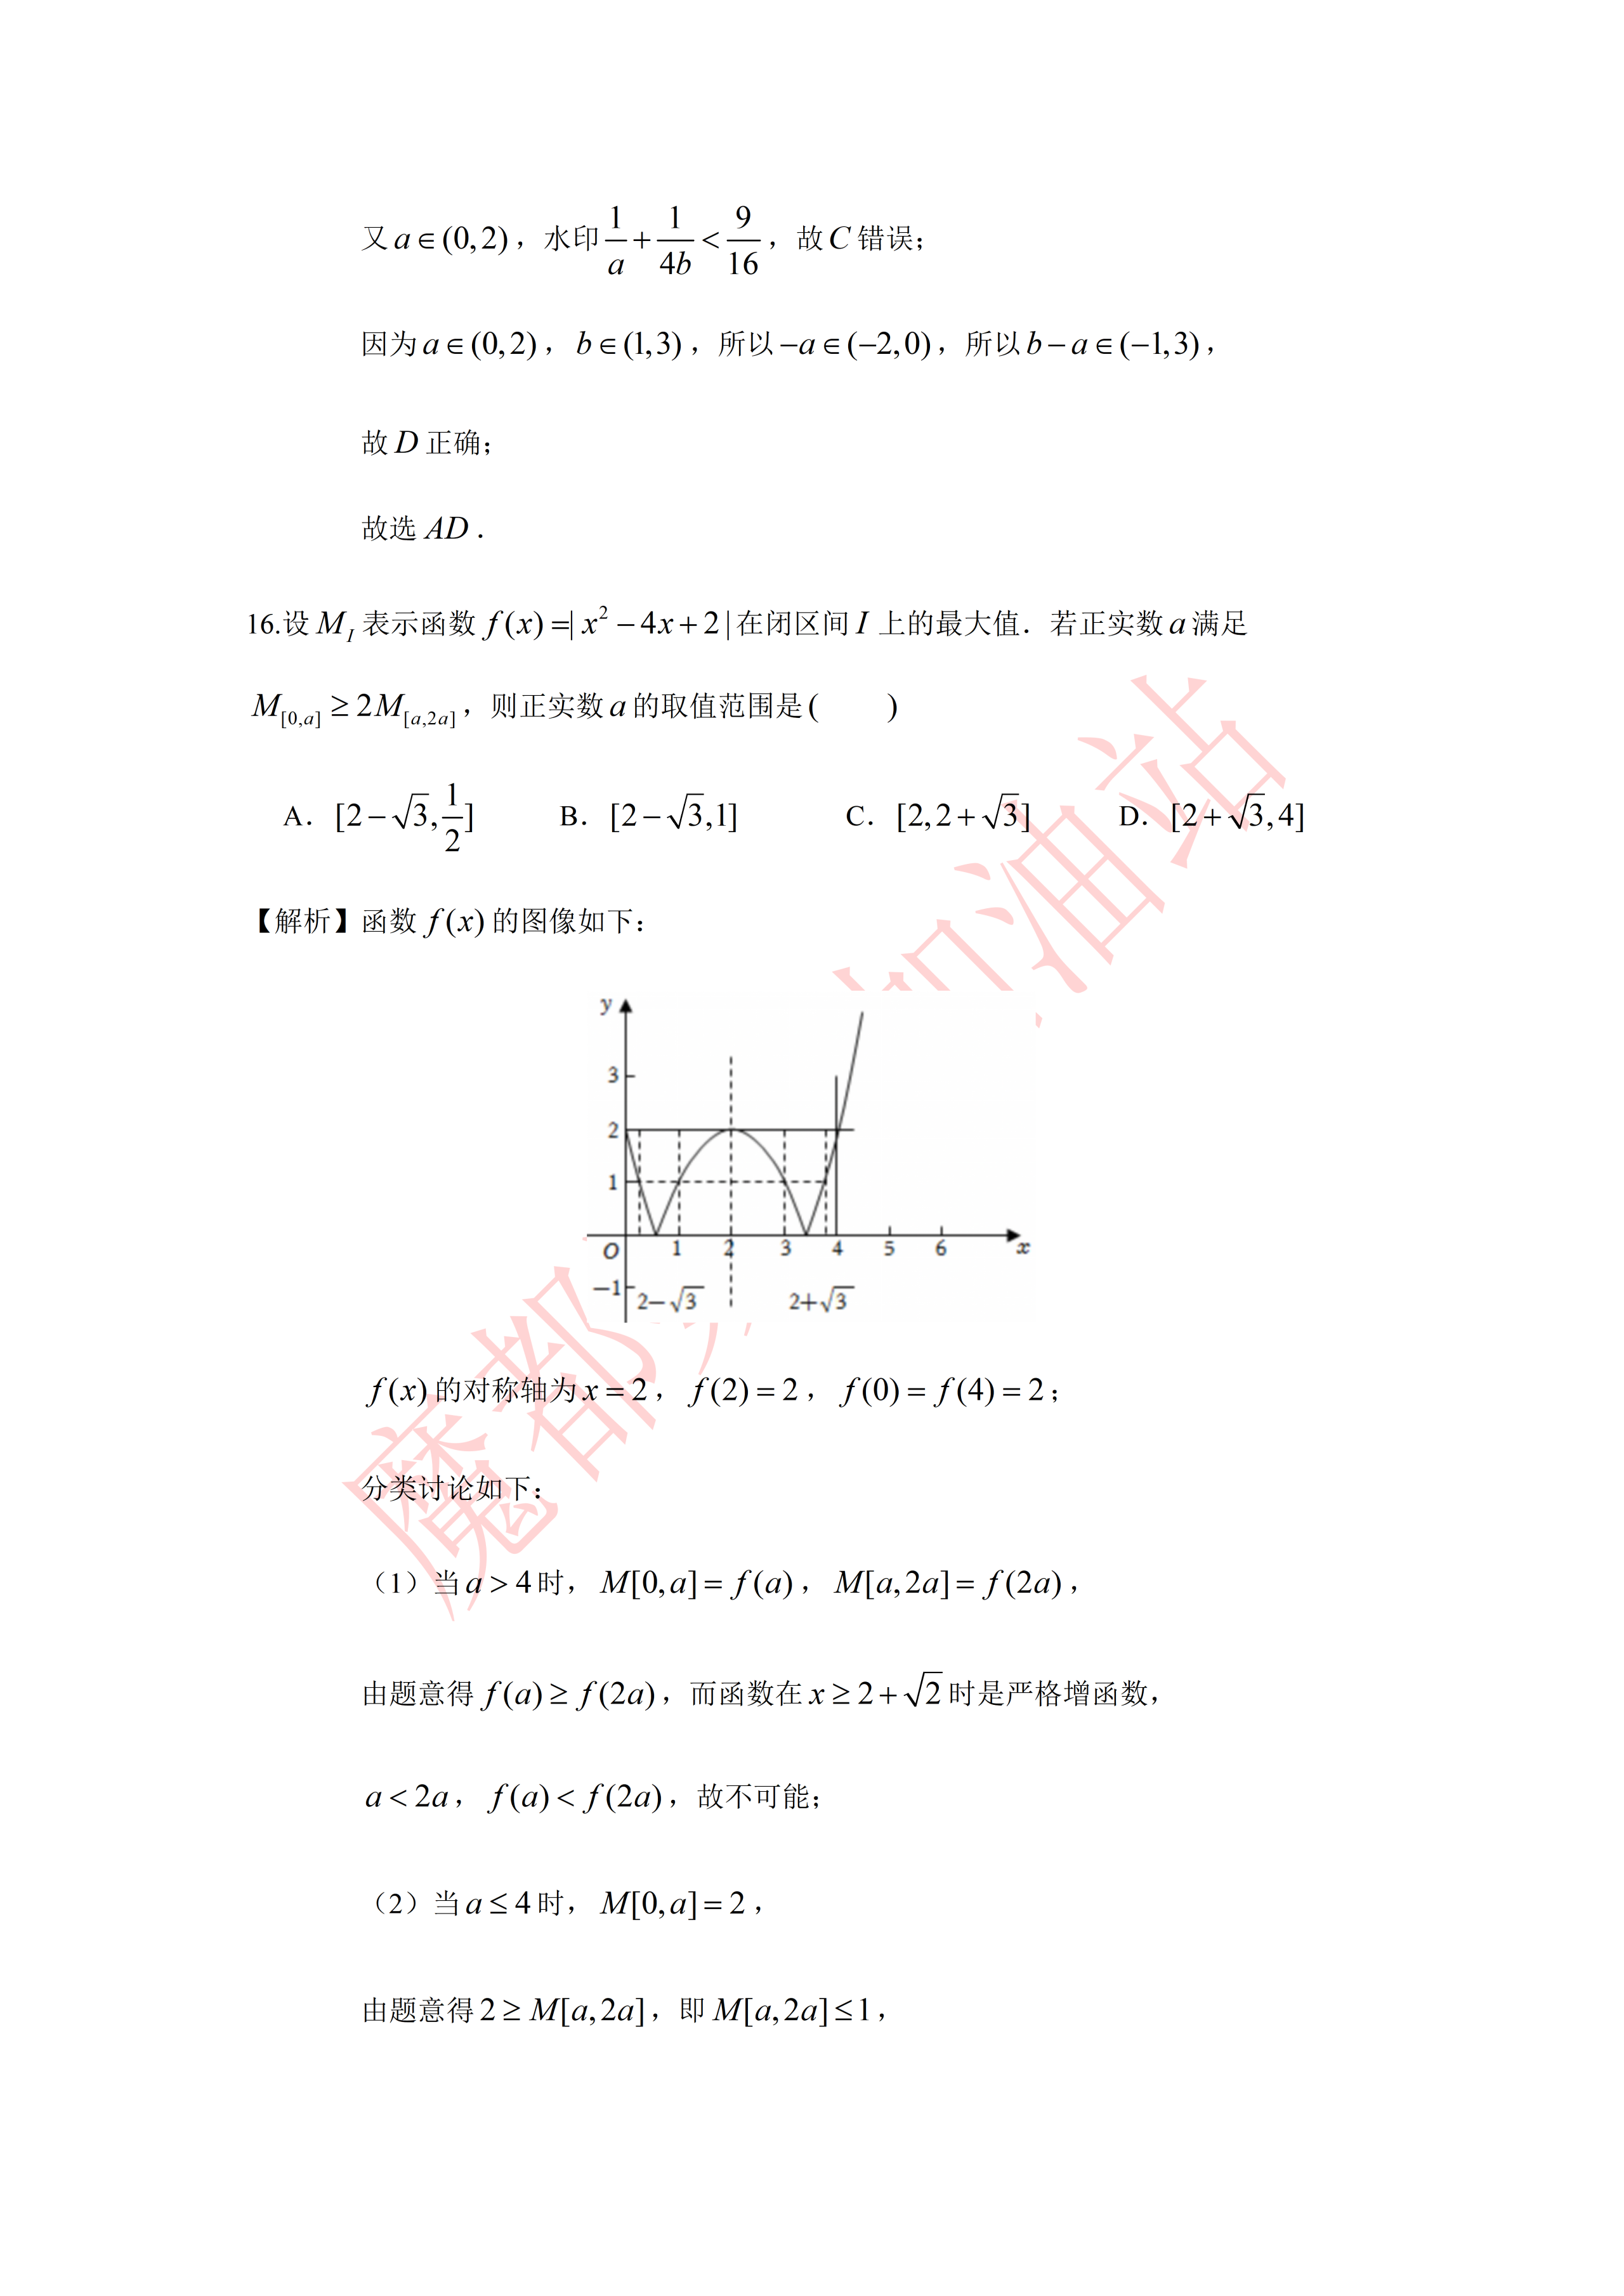
\includegraphics[width=.55\linewidth,trim=895bp 1535bp 915bp 1525bp,clip]{../原图/高一51_华师大二附中_国庆作业3/06.png}
\end{center}
\step{$f(x)$ 的对称轴为 $x=2$，$f(2)=2$，$f(0)=f(4)=2$；}
\step{分类讨论如下：}
\stepm{(1)}{当 $a>4$ 时，$M_{[0,a]}=f(a)$，$M_{[a,2a]}=f(2a)$，}
\step{由题意得 $f(a)\geqslant f(2a)$，而函数在 $x\geqslant2+\sqrt2$ 时是严格增函数，}
\step{$a<2a$，$f(a)<f(2a)$，故不可能；}
\stepm{(2)}{当 $a\leqslant4$ 时，$M_{[0,a]}=2$，}
\step{由题意得 $2\geqslant M_{[a,2a]}$，即 $M_{[a,2a]}\leqslant1$，}
\step{令 $f(x)=1$，解得 $x_1=2-\sqrt3$，$x_2=1$，$x_3=2+\sqrt3$，$x_4=3$，}
\step{则有 $a\geqslant2-\sqrt3$ 并且 $2a\leqslant1$，解得 $2-\sqrt3\leqslant a\leqslant\dfrac12$；}
\step{或者 $a\geqslant3$ 并且 $2a\leqslant2+\sqrt3$，无解；}
\step{故选 $A$.}
\solend

\fi

\end{enumerate}

\bigsec{三、解答题}

\begin{enumerate}
\setcounter{enumi}{16}

\item 已知 $M=\{x\mid2\leqslant x\leqslant5\}$，$N=\{x\mid a-1\leqslant x\leqslant2a+1\}$.
\begin{enumerate}[label=(\arabic*)]
\item 若 $M\subseteq N$，求实数 $a$ 的取值范围；
\item 若 $M\supseteq N$，求实数 $a$ 的取值范围.
\end{enumerate}

\ifanswer
\ans{（1）$[2,3]$；（2）$(-\infty,-2)$}
\fi

\ansspace[6]

\item 设集合 $A=\{x\mid|x+1|\leqslant3\}$，$B=\{x\mid0<x<3m\}$.
\begin{enumerate}[label=(\arabic*)]
\item 若 $A\cup B=A$，求实数 $m$ 的取值范围；
\item 设 $P=(\complement_R A)\cap B$，若 $\exists x\in\Z$ 且 $x\in P$，求实数 $m$ 的取值范围.
\end{enumerate}

\ifanswer
\solbegin
\stepm{(1)}{$A=\{x\mid|x+1|\leqslant3\}=\{x\mid-4\leqslant x\leqslant2\}$，且 $A\cup B=A$，所以 $B\subseteq A$.}
\step{若 $B=\varnothing$，此时 $0\geqslant3m$，解得 $m\leqslant0$；}
\step{若 $B\neq\varnothing$，此时 $0<3m$，且 $3m\leqslant2$，解得 $0<m\leqslant\dfrac23$；}
\step{则实数 $m$ 的取值范围是 $\left(-\infty,\dfrac23\right]$.}
\stepm{(2)}{因为 $\exists x\in\Z$ 且 $x\in P$，所以集合 $P$ 中至少存在一个整数.}
\step{$\complement_R A=\{x\mid x<-4\text{ 或 }x>2\}$，$B=\{x\mid0<x<3m\}$，}
\step{要使 $P=(\complement_R A)\cap B$ 中至少存在一个整数，则 $\begin{cases}3m>0\\3m>3\end{cases}$，解得 $m>1$，}
\step{则实数 $m$ 的取值范围是 $(1,+\infty)$.}
\solend

\fi

\ansspace[7]

\item 已知函数 $f(x)=x^2+(1-a)x-a(a\in\R)$.
\begin{enumerate}[label=(\arabic*)]
\item 解关于 $x$ 的不等式 $f(x)<0$；
\item 若 $\forall a\in[-1,1]$，$f(x)\geqslant0$ 恒成立，求实数 $x$ 的取值范围.
\end{enumerate}

\ifanswer
\solbegin
\stepm{(1)}{不等式 $x^2+(1-a)x-a<0$ 等价于 $(x-a)(x+1)<0$，}
\step{当 $a<-1$ 时，不等式的解集为 $(a,-1)$；}
\step{当 $a=-1$ 时，不等式的解集为 $\varnothing$；}
\step{当 $a>-1$ 时，不等式的解集为 $(-1,a)$.}
\stepm{(2)}{$x^2+(1-a)x-a=-a(x+1)+x^2+x$，}
\step{设 $g(a)=-a(x+1)+x^2+x$，$a\in[-1,1]$，}
\step{要使 $g(a)\geqslant0$ 在 $a\in[-1,1]$ 上恒成立，}
\step{只需 $\begin{cases}g(-1)\geqslant0\\g(1)\geqslant0\end{cases}$，即 $\begin{cases}x^2+2x+1\geqslant0\\x^2-1\geqslant0\end{cases}$，解得 $x\geqslant1$ 或 $x\leqslant-1$，}
\step{所以 $x$ 的取值范围为 $\{x\mid x\leqslant-1\text{ 或 }x\geqslant1\}$.}
\solend

\fi

\ansspace[7]

\item 若实数 $x$、$y$、$m$ 满足 $|x-m|>|y-m|$，则称 $x$ 比 $y$ 远离 $m$.
\begin{enumerate}[label=(\arabic*)]
\item 若 $2$ 比 $3x-4$ 远离 $1$，求 $x$ 的取值范围；
\item 设 $y=\dfrac{x+2}{x+1}$，其中 $x\in(0,\sqrt2)\cup(\sqrt2,+\infty)$，判断：$x$ 与 $y$ 哪一个更远离 $\sqrt2$？并说明理由.
\item 若 $x+y=2$，试问：$y$ 与 $x^2+y^2$ 哪一个更远离 $\dfrac12$？并说明理由.
\end{enumerate}

\ifanswer
\solbegin
\stepm{(1)}{由题意得 $|2-1|>|3x-4-1|$，所以 $|3x-5|<1$，解得 $\dfrac43<x<2$，}
\step{故 $x$ 的取值范围为 $\left(\dfrac43,2\right)$；}
\stepm{(2)}{$x$ 比 $y$ 更远离 $\sqrt2$，}
\step{理由如下：要证 $x$ 比 $y$ 更远离 $\sqrt2$，只要证 $|x-\sqrt2|>\left|\dfrac{x+2}{x+1}-\sqrt2\right|$，}
\step{即证 $|x-\sqrt2|>\left|\dfrac{(1-\sqrt2)(x-\sqrt2)}{x+1}\right|$，}
\step{因为 $x\in(0,\sqrt2)\cup(\sqrt2,+\infty)$，所以 $|x-\sqrt2|>0$，}
\step{所以只要证 $1>\dfrac{\sqrt2-1}{|x+1|}$，即证 $|x+1|>\sqrt2-1$，}
\step{因为 $x\in(0,\sqrt2)\cup(\sqrt2,+\infty)$，所以 $x+1\in(1,\sqrt2+1)\cup(\sqrt2+1,+\infty)$，}
\step{所以 $|x+1|>1>\sqrt2-1$，所以 $x$ 比 $y$ 更远离 $\sqrt2$；}
\stepm{(3)}{因为 $x^2+y^2\geqslant\dfrac{(x+y)^2}{2}=2$，当且仅当 $x=y=1$ 时等号成立，}
\step{所以 $\left|x^2+y^2-\dfrac12\right|=x^2+y^2-\dfrac12$，}
\step{从而 $\left|y-\dfrac12\right|-\left|x^2+y^2-\dfrac12\right|=\left|y-\dfrac12\right|-\left(x^2+y^2-\dfrac12\right)$，}
\step{①$y\geqslant\dfrac12$，$\left|y-\dfrac12\right|-\left|x^2+y^2-\dfrac12\right|=y-\dfrac12-\left(x^2+y^2-\dfrac12\right)=y-x^2-y^2$}
\step{$=y-(2-y)^2-y^2=-2y^2+5y-4=-2\left(y-\dfrac54\right)^2-\dfrac78<0$，}
\step{即 $\left|y-\dfrac12\right|<\left|x^2+y^2-\dfrac12\right|$；}
\step{②$y<\dfrac12$，}
\step{$\left|y-\dfrac12\right|-\left|x^2+y^2-\dfrac12\right|=\left(\dfrac12-y\right)-\left(x^2+y^2-\dfrac12\right)=-y-x^2-y^2+1$}
\step{$=-y-(2-y)^2-y^2+1=-2y^2+3y-3=-2\left(y-\dfrac34\right)^2-\dfrac{15}8<0$，}
\step{即 $\left|y-\dfrac12\right|<\left|x^2+y^2-\dfrac12\right|$；}
\step{综上，$\left|y-\dfrac12\right|<\left|x^2+y^2-\dfrac12\right|$，即 $x^2+y^2$ 比 $y$ 更远离 $\dfrac12$.}
\solend

\fi

\ansspace[9]

\item 对于非空有限整数集 $X$，$m\in\N^*$，定义 $X^m=\{x^m\mid x\in X\}$，对 $n\in\Z$，
$Y\oplus n=\{x+n\mid x\in Y\}$ 现有两个非空有限整数集 $A$、$B$，已知 $A\oplus1\subseteq B$ 且
$B^2\oplus(-4)\subseteq A$.
\begin{enumerate}[label=(\arabic*)]
\item 当 $A=\{-3,0\}$ 时求集合 $B$；
\item 证明：$A\subseteq\{-3,-2,0,1\}$；
\item 当 $A\oplus1=B$ 且 $B^2\oplus(-4)=A$ 时，任取 $a\in A$，$b\in B$ 构造函数
$f(x)=(x-a)(x-b)$ 问：当 $a$、$b$ 取何值时，$f(x)$ 的最小值最小？
\end{enumerate}

\ifanswer
\solbegin
\stepm{(1)}{因为 $A=\{-3,0\}$，$B^2\oplus(-4)\subseteq A$，}
\step{所以 $B^2\oplus(-4)$ 可能为 $\varnothing$、$\{-3\}$、$\{0\}$、$\{-3,0\}$，}
\step{当 $B^2\oplus(-4)=\varnothing$ 时 $B^2=\varnothing$，不满足非空，不合题意；}
\step{当 $B^2\oplus(-4)=\{-3\}$ 时 $B^2=\{1\}$，所以 $B=\{1,-1\}$、$\{1\}$、$\{-1\}$，}
\step{当 $B^2\oplus(-4)=\{0\}$ 时 $B^2=\{4\}$，所以 $B=\{2,-2\}$、$\{2\}$、$\{-2\}$，}
% 原卷如此，照录未改（此处作 $\{0,-3\}$，上一行同一集合作 $\{-3,0\}$）
\step{当 $B^2\oplus(-4)=\{0,-3\}$ 时 $B^2=\{4,1\}$，}
\step{所以 $B=\{1,2,-1,-2\}$、$\{2,-1,-2\}$、$\{2,1,-2\}$、$\{1,-1,-2\}$、$\{1,-1,2\}$、$\{1,2\}$、$\{-1,2\}$、$\{-1,-2\}$、$\{1,-2\}$，}
\step{又 $A\oplus1=\{-2,1\}\subseteq B$，得 $B$ 为 $\{1,-2\}$、$\{2,1,-2\}$、$\{1,-1,-2\}$、$\{1,2,-1,-2\}$.}
\stepm{(2)}{设 $x\in A$，因为 $A\oplus1\subseteq B$，所以 $x+1\in B$，}
\step{又 $B^2\oplus(-4)\subseteq A$，所以 $(x+1)^2-4\in A$，}
% 原卷如此，照录未改（此处及下文取 $x=2$ 处原卷均作 $(-4+1)^2-4=52-2a>0$）
\step{取 $x=-4$，则 $(-4+1)^2-4=52-2a>0$，$(5+1)^2-4=32\in A$，$\cdots$，}
\step{无限迭代，而 $A$ 为有限集，不合题意，舍去，即 $-4\notin A$；}
\step{取 $x=-3$，则 $(-3+1)^2-4=0\in A$，$(0+1)^2-4=-3\in A$，}
\step{得 $A$ 集合可为 $\{-3,0\}$；}
\step{取 $x=-2$，则 $(-2+1)^2-4=-3\in A$，$(-3+1)^2-4=0\in A$，}
\step{$(0+1)^2-4=-3\in A$，得 $A$ 集合可为 $\{-3,-2,0\}$；}
\step{取 $x=-1$，则 $(-1+1)^2-4=-4\in A$，又 $-4\notin A$，所以 $-1\notin A$，}
\step{取 $x=1$，则 $(1+1)^2-4=0\in A$，$(0+1)^2-4=-3\in A$，}
\step{$(-3+1)^2-4=0\in A$，得 $A$ 集合可为 $\{-3,0,1\}$，}
\step{取 $x=2$，则 $(2+1)^2-4=52-2a>0$，$(5+1)^2-4=32\in A$，$\cdots$，}
\step{无限迭代，而 $A$ 为有限集，不合题意，舍去，即 $2\notin A$，}
\step{同理当 $x<-4$ 或 $x>2$，且 $x\in\Z$ 时不符合 $A$ 为有限集，舍去；}
\step{故由上得 $A$ 集合可为 $\{-3,0\},\{-3,-2,0\},\{-3,0,1\},\{-3,-2,0,1\}$，}
\step{所以 $A\subseteq\{-3,-2,0,1\}$，}
\stepm{(3)}{当 $A\oplus1=B$ 且 $B^2\oplus(-4)=A$ 时，}
\step{设 $x\in B$，则 $x^2-4\in B^2\oplus(-4)=A$，}
% 原卷如此，照录未改（题设 $A=\{-3,0\}$，此处两个判别式取的是 $-2$ 与 $1$，均不属于 $A$）
\step{$x^2-4=-2$ 时 $x=\pm\sqrt2$，不为整数，不合题意；}
\step{$x^2-4=1$ 时 $x=\pm\sqrt5$，不为整数，不合题意；}
\step{所以 $A=\{-3,0\}$，又 $A\oplus1=B$，则 $B=\{-2,1\}$，}
\step{任取 $a\in A$，$b\in B$ 构造函数 $f(x)=(x-a)(x-b)$，}
\step{$f(x)=(x-a)(x-b)=x^2-(a+b)x+ab$}
\step{$=x^2-(a+b)x+\dfrac{(a+b)^2}{4}+ab-\dfrac{(a+b)^2}{4}$}
\step{$=\left[x-\dfrac{(a+b)}2\right]^2-\dfrac{(a-b)^2}{4}\geqslant-\dfrac{(a-b)^2}{4}$，所以 $f(x)_{min}=-\dfrac{(a-b)^2}{4}$，}
\step{又 $a\in A=\{-3,0\}$，$b\in B=\{-2,1\}$，所以 $a-b$ 的取值有 $-1,-4,2$，}
\step{所以 $f(x)_{min}=-\dfrac{(a-b)^2}{4}\geqslant-\dfrac{(-3-1)^2}{4}=-4$，}
\step{即当 $a=-3$，$b=1$ 时 $f(x)_{min}$ 的最小值为 $-4$.}
\solend

\fi

\ansspace*[12]

\end{enumerate}

\end{document}
"
% 紧凑版：xelatex "\def\iscompact{1}% 高一51_华师大二附中_国庆作业3.tex
%   —— 高一上数学“2026-2027 年华师大二附中高一上国庆作业 3”（讲评版）
% 试卷版：xelatex 高一51_华师大二附中_国庆作业3.tex
% 答案版：xelatex "\def\isanswer{1}% 高一51_华师大二附中_国庆作业3.tex
%   —— 高一上数学“2026-2027 年华师大二附中高一上国庆作业 3”（讲评版）
% 试卷版：xelatex 高一51_华师大二附中_国庆作业3.tex
% 答案版：xelatex "\def\isanswer{1}% 高一51_华师大二附中_国庆作业3.tex
%   —— 高一上数学“2026-2027 年华师大二附中高一上国庆作业 3”（讲评版）
% 试卷版：xelatex 高一51_华师大二附中_国庆作业3.tex
% 答案版：xelatex "\def\isanswer{1}\input{高一51_华师大二附中_国庆作业3.tex}"
% 紧凑版：xelatex "\def\iscompact{1}\input{高一51_华师大二附中_国庆作业3.tex}"
%
% 原始材料：微信公众号“魔都数学加油站”文章，作者破晓，连载“27学年高一51”；
% 原文标题“27学年高一51——2026-2027年上海市华师大二附中高一上国庆作业3”；
% 原文链接：https://mp.weixin.qq.com/s/95SLMEmPUT30s4U7wjr5Og。
% 该页面用 JS 渲染，未见明确发布日期；页面内时间戳约为 2026-10-05 21:37，本稿以该时刻记可得日期。
% 正文为 12 张 PNG 页：第 01、02、03、05、07、08、11 页 4762×6735，
% 第 04、06、09、10、12 页 2560×3620。按页序逐页读取，12 页全为试卷正文页
% （卷首标题在第 1 页页顶，卷末解答题止于第 12 页），无封面页、目录页或单独的页脚页。
% 卷面标题照原卷印作“2026-2027 年华师大二附中高一上国庆作业 3”（公众号标题中的“上海市”
% 卷面标题行没有，本稿照卷面），年份区间按全稿惯例排 en dash。
%
% 篇幅与题号：原卷自第 3 题起编号（第 1、2 题不在本卷内）。填空题 3—12（10 题）、
% 选择题 13—16（4 题）、解答题 17—21（5 题），共 19 题。本稿沿用原节与原题号，
% 只改排为全稿统一的大节样式（原卷小节标题为“一、填空题”“二、选择题”“三、解答题”）。
% 正文为讲评版：填空题 3—12 与选择题 13—16 只印【解析】（选择题的结论“故选 X”印在解析内），
% 按全稿口径这类题不另提 \ans{}；解答题第 17 题只印【答案】，故只给 \ans{}；
% 第 18—21 题只印【解析】。
%
% 副标题：原卷未印副标题。本稿按“知识模块”口径标作“集合与常用逻辑用语、不等式”：
% 19 题中集合与常用逻辑用语 8 题（3、4、6、10、13、17、18、21），
% 不等式（含函数最值、绝对值不等式）11 题（5、7、8、9、11、12、14、15、16、19、20），
% 两类均远超三分之一，故并标。口径同 高一46_交附闵行_国庆作业3、高一48_华师大二附中_周末作业2。
%
% 与原卷的排版差异：
%   ① 原卷每题下直接印【答案】或【解析】，本稿按全稿惯例将答案与解析置于答案版；
%   ② 原卷未印副标题，本稿按“知识模块”口径补出；
%   ③ 原卷填空横线按全稿惯例排为 \blankline[4.4em]；
%   ④ 原卷 $R$、$N$、$Z$ 均排斜体，本稿按全稿惯例改用花体 $\R$、$\N$、$\Z$（同 高一48）；
%   ⑤ 原卷第 12 题解析配图、第 13 题题干韦恩图都印在正文右侧的浮动位置，第 16 题解析配图
%      印在解析行间；本稿三图一律居中排，均自原图对应页裁切（trim），不另存图片文件；
%   ⑥ 原卷解答题未留作答空白，本稿按全稿惯例加 \ansspace；
%   ⑦ 原卷第 15 题解析第 7、8 两个印刷行是一串连等式的折行，本稿按“一条 \step ＝ 一个印刷行”
%      的口径分成两条 \step。
%
% 原卷笔误/存疑（均照录未改，正文对应处另有 % 注）：
%   ① 第 12 题解析末行作“区间长度之和为 $x_1-b+x_2-a=x_1-x_2-a-b=2+a+b-a-b=2$”，
%      按上一行 $x_1+x_2=2+a+b$，此处应为 $x_1+x_2$；原卷作 $x_1-x_2$。
%   ② 第 15 题解析“又 $a\in(0,2)$，”与 $\dfrac1a+\dfrac1{4b}<\dfrac9{16}$ 之间，
%      原卷正文夹印“水印”二字（系制版遗留字样，非试卷内容）。
%   ③ 第 21 题第 (2) 问解析两处（取 $x=-4$、取 $x=2$）作“$=52-2a>0$”，
%      与题设 $(x+1)^2-4$ 的取值（按 $x=-4$ 应为 $5$）不符，当系原卷算式遗留。
%   ④ 第 21 题第 (1) 问解析先写 $B^2\oplus(-4)$ 可能为 $\{-3,0\}$，后文又作 $\{0,-3\}$，
%      同一集合两种写法。
%   ⑤ 第 21 题第 (3) 问解析：题设 $B^2\oplus(-4)=A$ 且 $A=\{-3,0\}$ 时，由 $x^2-4\in A$
%      应得 $x^2-4=-3$ 或 $0$；原卷讨论的却是 $x^2-4=-2$ 与 $x^2-4=1$（两值均不属于 $A$），
%      与题设不合。
%
% 插图：3 张，均自原图裁切（无 \begin{tikzpicture} 重排）：
%   · 第 13 题题干韦恩图（原图第 04 页，图在题干与选项右侧）
%   · 第 12 题解析配图（原图第 04 页，图在解析右侧）
%   · 第 16 题解析配图（原图第 06 页，图在解析中间）
%
\documentclass[a4paper,11pt]{article}
\usepackage{common}

\begin{document}

\examtitlest[3]{2026--2027 年华师大二附中高一上国庆作业 3}{集合与常用逻辑用语、不等式}

\bigsec{一、填空题}

\begin{enumerate}
\setcounter{enumi}{2}

\item 若 $\{x\mid x<1\text{ 或 }x>4\}\cup\{x\mid m<x<2m+3\}=R$，则实数 $m$ 的取值范围为\blankline[4.4em].

\ifanswer
\solbegin
\step{因为 $\{x\mid x<1\text{ 或 }x>4\}\cup\{x\mid m<x<2m+3\}=R$，}
\step{所以 $\begin{cases}m<1\\2m+3>4\end{cases}$，解得 $\dfrac12<m<1$，所以 $m$ 的取值范围为 $\left(\dfrac12,1\right)$.}
\solend

\fi

\item 若“$x\leqslant5$”是“$x<a$”的必要不充分条件，则 $a$ 的取值范围是\blankline[4.4em].

\ifanswer
\solbegin
\step{若“$x\leqslant5$”是“$x<a$”的必要不充分条件，则 $\{x\mid x<a\}\subset\{x\mid x\leqslant5\}$，}
\step{所以 $a\leqslant5$.}
\solend

\fi

\item 实数 $x$、$y$ 满足 $x^2+2xy+4y^2=1$，则 $x+2y$ 的取值范围是\blankline[4.4em].

\ifanswer
\solbegin
\step{因为 $x^2+2xy+4y^2=(x+2y)^2-2xy=1$，}
\step{所以 $(x+2y)^2-1=x\cdot(2y)\leqslant\left(\dfrac{x+2y}{2}\right)^2$，当且仅当 $x=2y$ 时取等号，}
\step{解得 $-\dfrac{2\sqrt3}{3}\leqslant x+2y\leqslant\dfrac{2\sqrt3}{3}$，故 $x+2y$ 的取值范围是 $\left[-\dfrac{2\sqrt3}{3},\dfrac{2\sqrt3}{3}\right]$.}
\solend

\fi

\item 若命题 $p$：“$\exists x\in\R$，$5x^2-3x+m=0$”为假命题，则实数 $m$ 的取值范围为\blankline[4.4em].

\ifanswer
\solbegin
\step{若命题 $p$：$\exists x\in\R$，$5x^2-3x+m=0$ 为假命题，}
\step{则 $5x^2-3x+m=0$ 没有实数根，故 $\Delta=9-20m<0$，解得 $m>\dfrac9{20}$.}
\solend

\fi

\item 若当 $3\leqslant m\leqslant5$ 时，$mx^2-mx+m-9<0$ 有解，则实数 $x$ 的取值范围是\blankline[4.4em].

\ifanswer
\solbegin
\step{当 $3\leqslant m\leqslant5$ 时，$mx^2-mx+m-9<0$ 有解，}
\step{即 $(x^2-x+1)m-9<0$ 在 $m\in[3,5]$ 上有解，}
\step{因为 $x^2-x+1>0$，所以一次函数 $g(m)=(x^2-x+1)m-9$ 严格增，}
\step{所以只需 $g(3)=3x^2-3x-6<0$ 即可，}
\step{即 $x^2-x-2<0$，$(x-2)(x+1)<0$，解得 $-1<x<2$，}
\step{所以实数 $x$ 的取值范围是 $(-1,2)$.}
\solend

\fi

\item 已知不等式 $\dfrac{x}{x^2+4}\leqslant a$ 对任意的 $x\in[1,3]$ 恒成立，则实数 $a$ 的范围为\blankline[4.4em].

\ifanswer
\solbegin
\step{因为 $x\in[1,3]$，所以 $\dfrac{x}{x^2+4}=\dfrac{1}{x+\dfrac4x}\leqslant\dfrac{1}{2\sqrt{x\times\dfrac4x}}=\dfrac14$，}
\step{当且仅当 $x=\dfrac4x$ 时，即 $x=2$ 时取等号，即 $\dfrac{x}{x^2+4}$ 在 $x\in[1,3]$ 的最大值为 $\dfrac14$，}
\step{又由不等式 $\dfrac{x}{x^2+4}\leqslant a$ 对任意的 $x\in[1,3]$ 恒成立，所以 $a\geqslant\dfrac14$，}
\step{即实数 $a$ 的范围为 $\left[\dfrac14,+\infty\right)$.}
\solend

\fi

\item 甲、乙两人解关于 $x$ 的不等式 $x^2+bx+c<0$，甲写错了 $b$，正确计算后得到的解为 $\{x\mid1<x<2\}$；
乙写错了 $c$，正确计算后得到的解为 $\{x\mid-4<x<1\}$. 那么不等式 $\dfrac{bx+c}{x-2}<0$ 的解为\blankline[4.4em].

\ifanswer
\solbegin
\step{由 $x^2+bx+c<0$ 的解为 $\{x\mid1<x<2\}$，}
\step{则 $1$ 和 $2$ 是方程 $x^2+bx+c=0$ 的两个根，}
\step{甲写错了 $b$，但 $c$ 是正确的，所以 $c=1\times2=2$；}
\step{由 $x^2+bx+c<0$ 的解为 $\{x\mid-4<x<1\}$，}
\step{则 $-4$ 和 $1$ 是方程 $x^2+bx+c=0$ 的两个根，}
\step{乙写错了 $c$，但 $b$ 是正确的，所以 $-b=-4+1=-3$，即 $b=3$.}
\step{由 $\dfrac{bx+c}{x-2}<0$，得 $\dfrac{3x+2}{x-2}<0$，即 $(3x+2)(x-2)<0$，解得 $-\dfrac23<x<2$.}
\step{不等式 $\dfrac{bx+c}{x-2}<0$ 的解为 $\left\{x\mid-\dfrac23<x<2\right\}$.}
\solend

\fi

\item 已知 $\dfrac{1}{x-2}\geqslant1$ 是 $|x-a|<2$ 的充分非必要条件，则实数 $a$ 的取值范围是\blankline[4.4em].

\ifanswer
\solbegin
\step{由 $\dfrac{1}{x-2}\geqslant1$ 得 $\dfrac{3-x}{x-2}\geqslant0$，解得 $2<x\leqslant3$，由 $|x-a|<2$ 得 $a-2<x<a+2$，}
\step{因为 $\dfrac{1}{x-2}\geqslant1$ 是 $|x-a|<2$ 的充分非必要条件，}
\step{所以 $\{x\mid2<x\leqslant3\}\subset\{x\mid a-2<x<a+2\}$，所以 $\begin{cases}a-2\leqslant2\\a+2>3\end{cases}$，解得 $1<a\leqslant4$，}
\step{即实数 $a$ 的取值范围是 $(1,4]$.}
\solend

\fi

\item 设 $a>0$，$b>0$，若不等式 $a(a+1)^2+b(b+1)^2\geqslant\lambda ab$ 恒成立，则实数 $\lambda$ 的最大值为\blankline[4.4em].

\ifanswer
\solbegin
\step{$a(a+1)^2+b(b+1)^2\geqslant\lambda ab\Leftrightarrow\lambda\leqslant\dfrac{a(a+1)^2+b(b+1)^2}{ab}=\dfrac{(a+1)^2}{b}+\dfrac{(b+1)^2}{a}$，}
\step{从而原问题转化为求 $\dfrac{(a+1)^2}{b}+\dfrac{(b+1)^2}{a}$ 的最小值.}
\step{因为 $\dfrac{(a+1)^2}{b}+\dfrac{(b+1)^2}{a}=\dfrac{b^2+2b+1}{a}+\dfrac{a^2+2a+1}{b}$}
\step{$=\left(\dfrac{b^2}{a}+\dfrac{a^2}{b}\right)+2\left(\dfrac ba+\dfrac ab\right)+\left(\dfrac1a+\dfrac1b\right)\geqslant2\sqrt{\dfrac{b^2}{a}\cdot\dfrac{a^2}{b}}+2\times2\sqrt{\dfrac ba\cdot\dfrac ab}+2\sqrt{\dfrac1a\cdot\dfrac1b}$}
\step{$=2\sqrt{ab}+4+\dfrac{2}{\sqrt{ab}}\geqslant2\sqrt{2\sqrt{ab}\cdot\dfrac{2}{\sqrt{ab}}}+4=8$，以上均当且仅当 $a=b$ 时取等号，}
\step{所以 $\lambda\leqslant8$，即实数 $\lambda$ 的最大值为 $8$.}
\solend

\fi

\item 定义区间 $(a,d)$、$[a,d)$、$(a,d]$、$[a,d]$ 的长度为 $d-a$（$d>a$），已知 $a>b$，则满足
$\dfrac{1}{x-a}+\dfrac{1}{x-b}\geqslant1$ 的 $x$ 构成的区间的长度之和为\blankline[4.4em].

\ifanswer
\solbegin
\step{因为 $\dfrac{1}{x-a}+\dfrac{1}{x-b}\geqslant1$，所以 $\dfrac{2x-(a+b)}{(x-a)(x-b)}\geqslant1$，}
\step{即 $\dfrac{2x-(a+b)}{(x-a)(x-b)}-1\geqslant0$，则 $\dfrac{x^2-(2+a+b)x+ab+a+b}{(x-a)(x-b)}\leqslant0$，}
\step{设 $x^2-(2+a+b)x+ab+a+b=0$ 的根为 $x_1$ 和 $x_2$，}
\begin{center}
% 原卷该图印在解析右侧（原图第 04 页），本稿移作居中排，直接裁取原图，不另存图片文件。
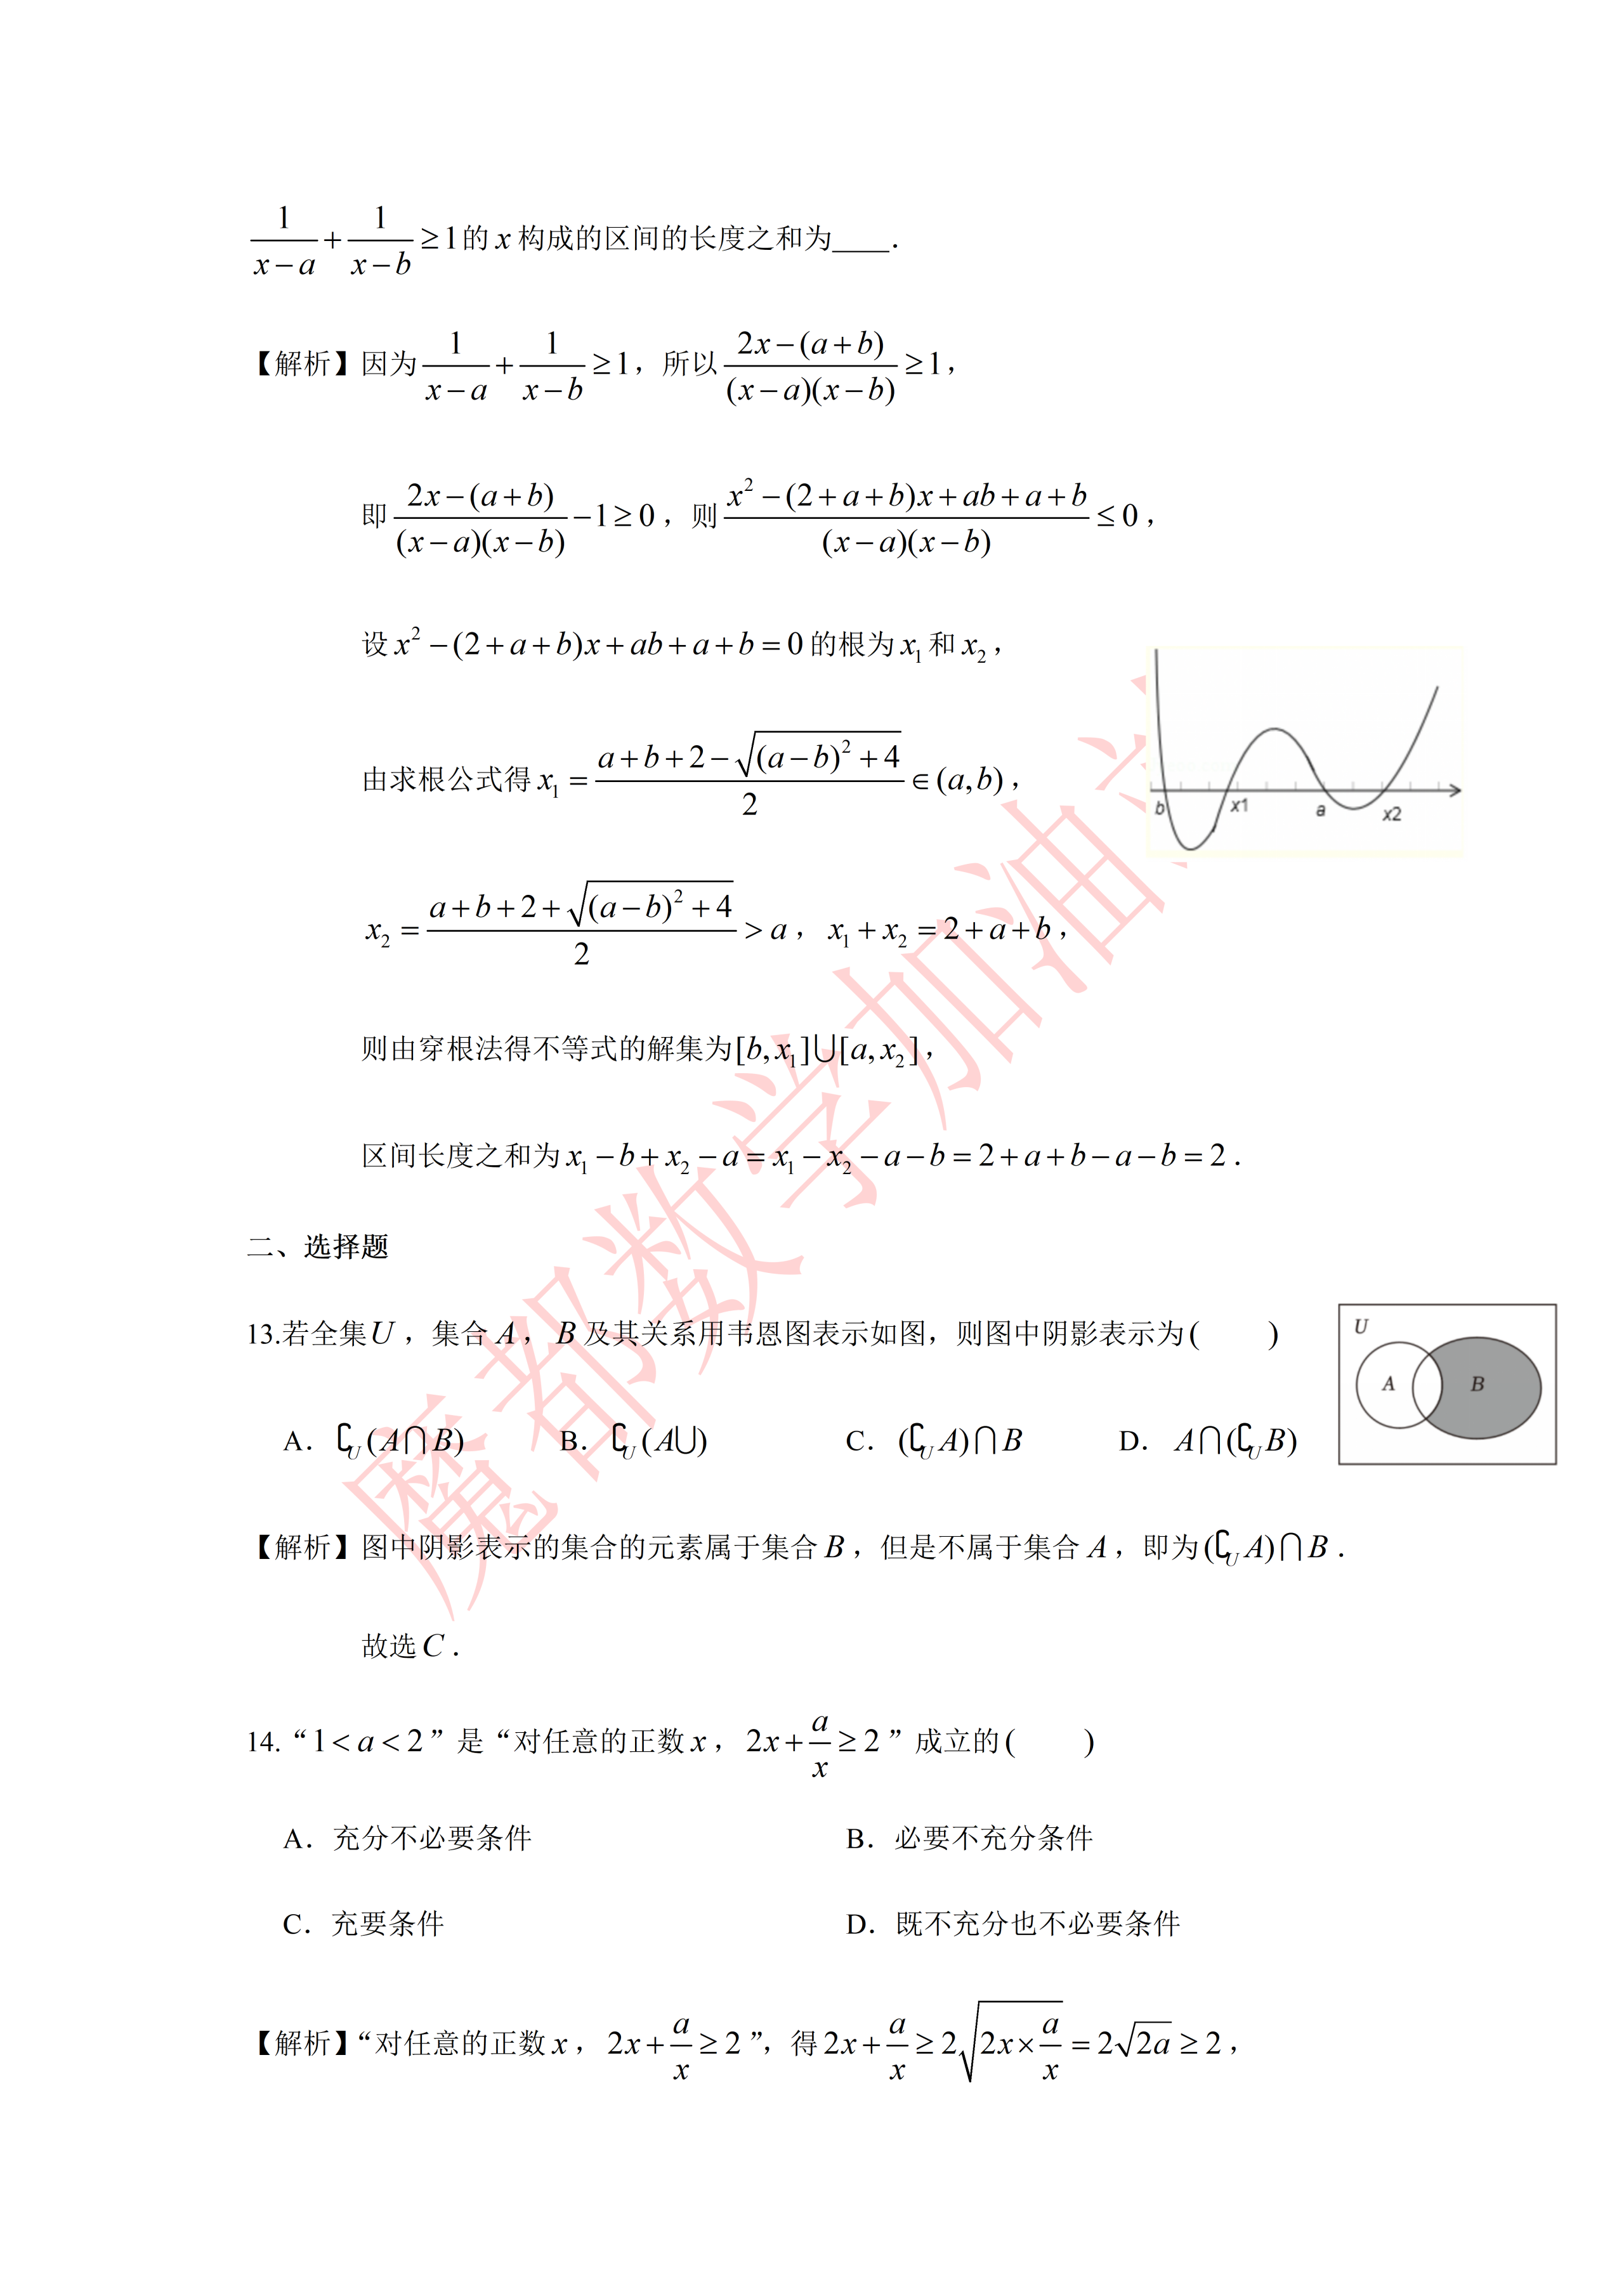
\includegraphics[width=.50\linewidth,trim=1786bp 2255bp 228bp 985bp,clip]{../原图/高一51_华师大二附中_国庆作业3/04.png}
\end{center}
\step{由求根公式得 $x_1=\dfrac{a+b+2-\sqrt{(a-b)^2+4}}{2}\in(a,b)$，}
\step{$x_2=\dfrac{a+b+2+\sqrt{(a-b)^2+4}}{2}>a$，$x_1+x_2=2+a+b$，}
\step{则由穿根法得不等式的解集为 $[b,x_1]\cup[a,x_2]$，}
% 原卷如此，照录未改（此处原卷作 $x_1-x_2$，按上一行 $x_1+x_2=2+a+b$ 当为 $x_1+x_2$）
\step{区间长度之和为 $x_1-b+x_2-a=x_1-x_2-a-b=2+a+b-a-b=2$.}
\solend

\fi

\end{enumerate}

\bigsec{二、选择题}

\begin{enumerate}
\setcounter{enumi}{12}

% 本题是“题干 + 图 + 选项”约 5.5cm 的一整块，图夹在题干与选项之间时 \keepwithprev 挡不住断点，
% 故按 高一30 第 13 题的成例在题前先量一次页高（守卫放在 \item 之前）。
\needvspace{6cm}
\item 若全集 $U$，集合 $A$、$B$ 及其关系用韦恩图表示如图，则图中阴影表示为\mbox{（\quad）}

\begin{center}
% 原卷该图印在题干与选项右侧（原图第 04 页），本稿移作居中排，直接裁取原图，不另存图片文件。
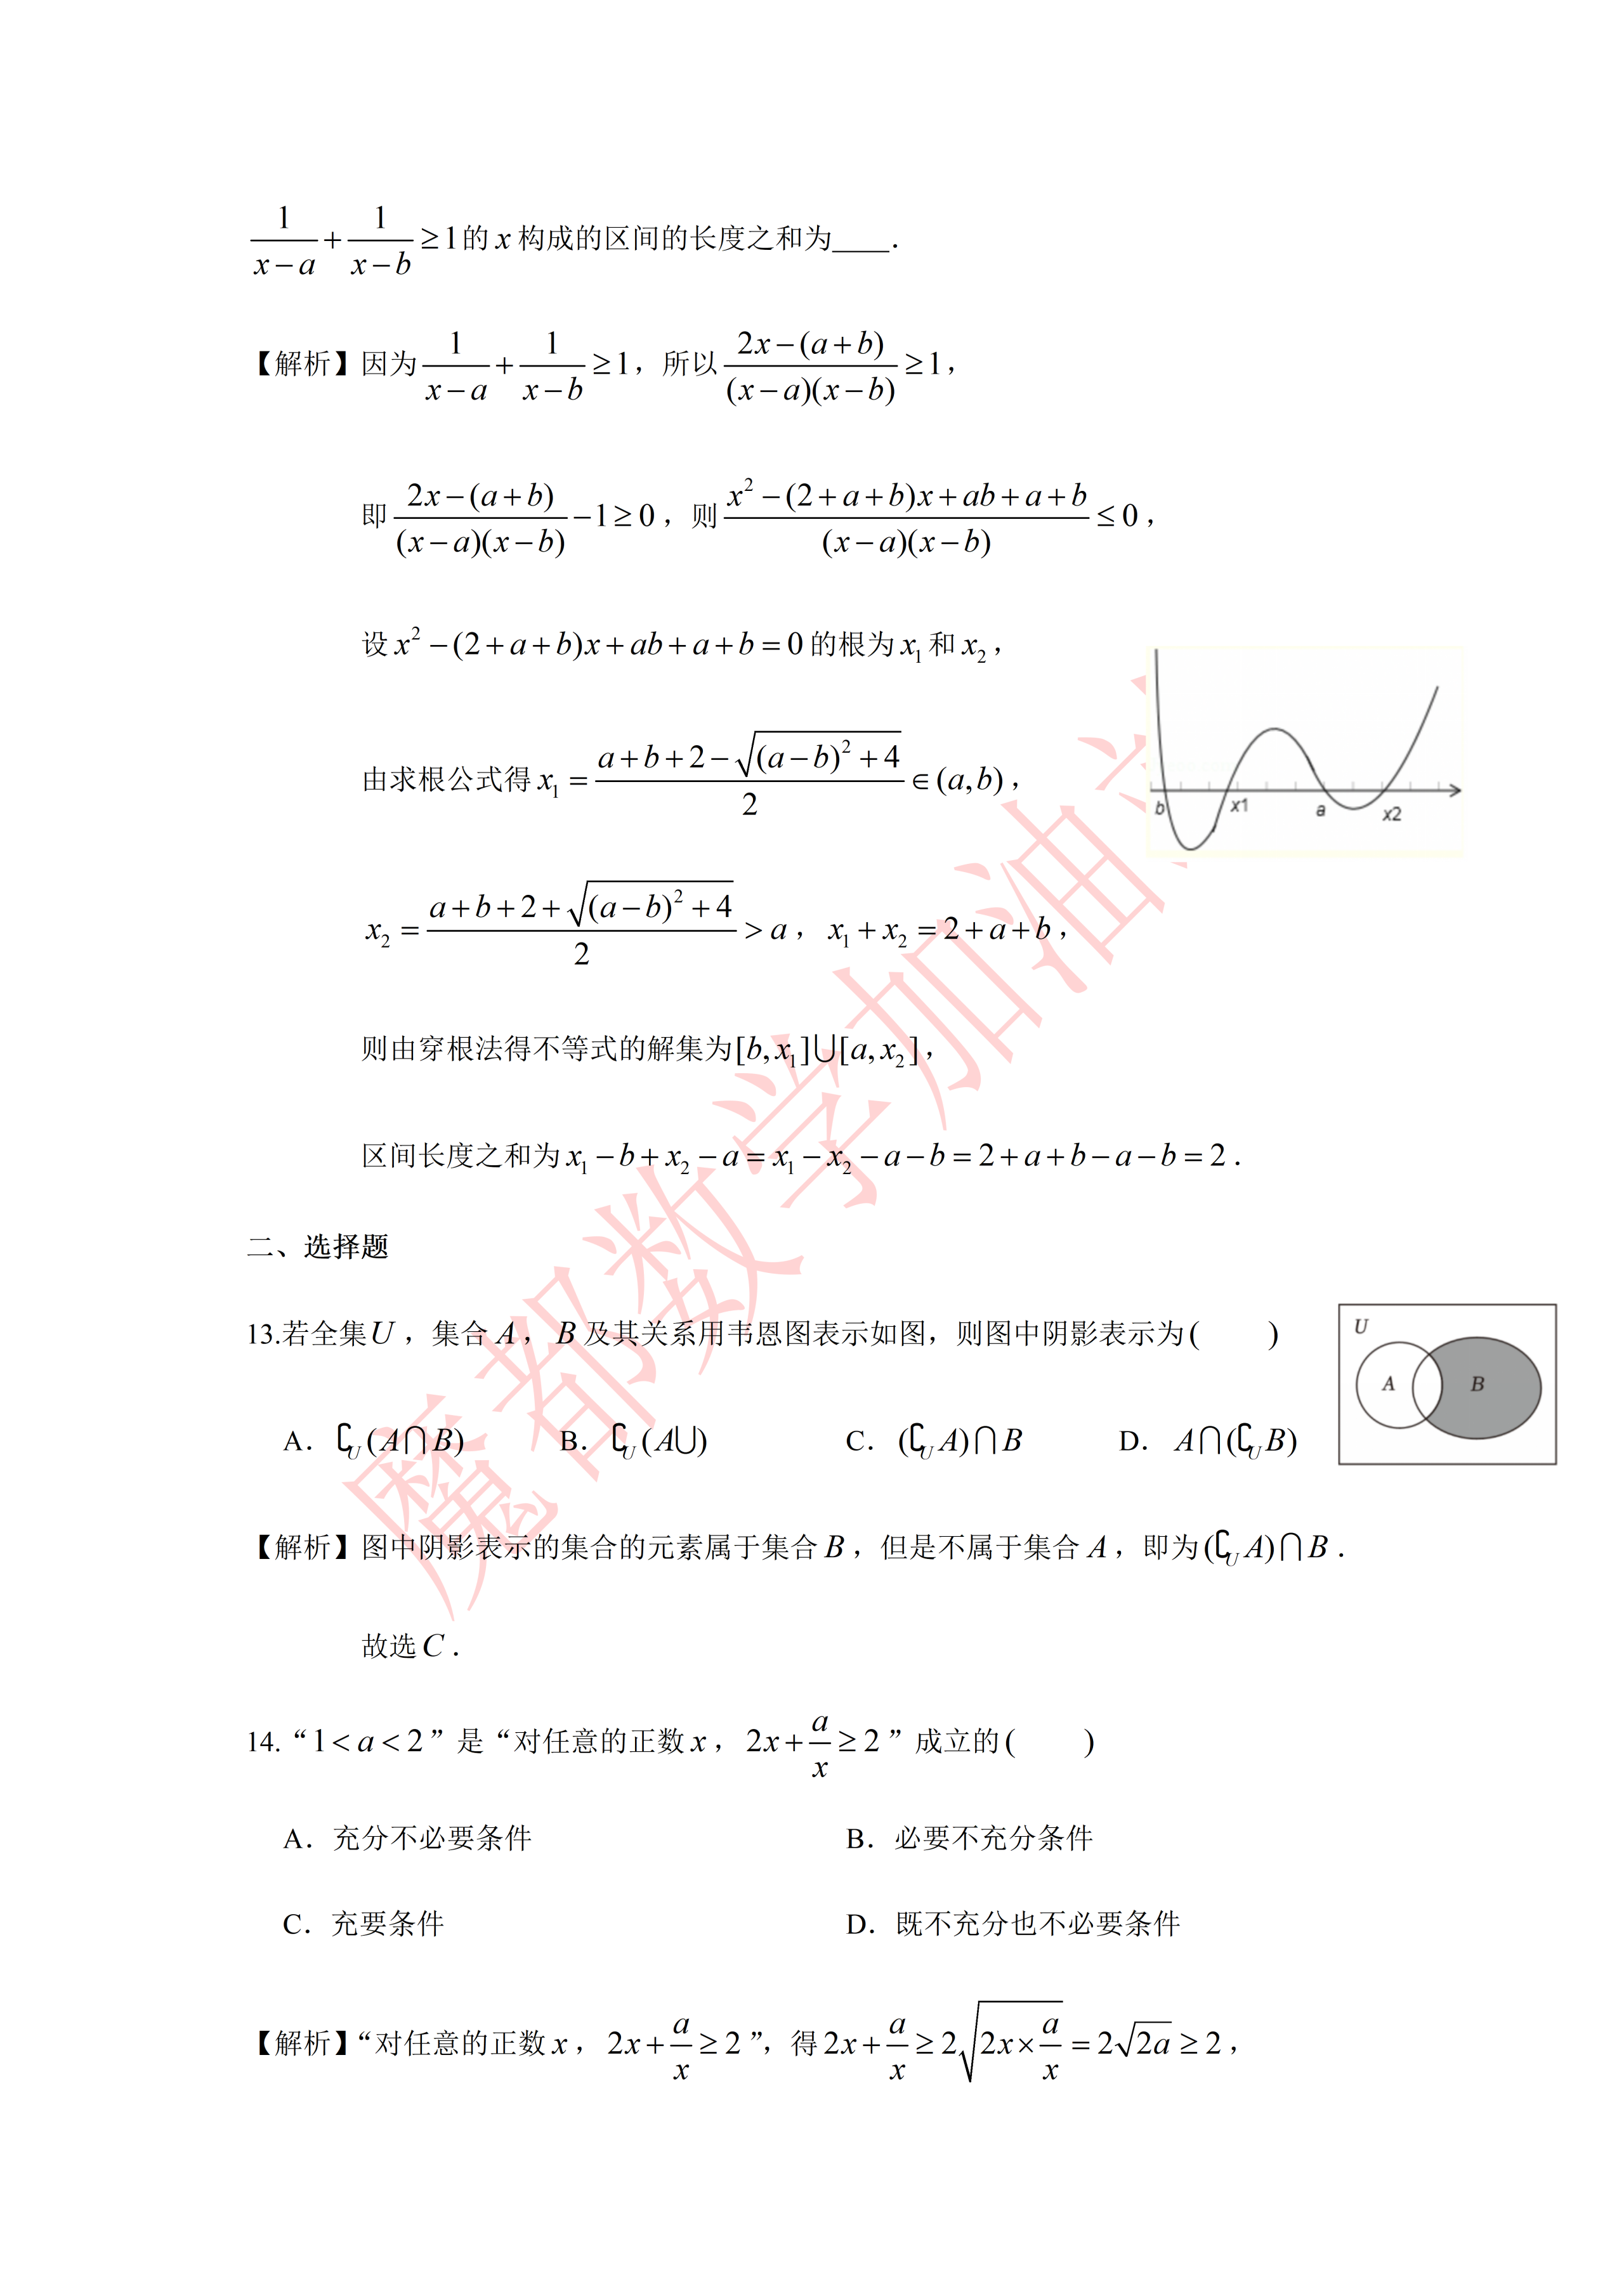
\includegraphics[width=.30\linewidth,trim=2105bp 1308bp 105bp 2050bp,clip]{../原图/高一51_华师大二附中_国庆作业3/04.png}
\end{center}

\keepwithprev
A. $\complement_U(A\cap B)$\qquad B. $\complement_U(A\cup B)$

C. $(\complement_U A)\cap B$\qquad D. $A\cap(\complement_U B)$

\ifanswer
\solbegin
\step{图中阴影表示的集合的元素属于集合 $B$，但是不属于集合 $A$，即为 $(\complement_U A)\cap B$.}
\step{故选 $C$.}
\solend

\fi

\item “$1<a<2$”是“对任意的正数 $x$，$2x+\dfrac ax\geqslant2$”成立的\mbox{（\quad）}

\keepwithprev
A. 充分不必要条件\qquad B. 必要不充分条件

C. 充要条件\qquad\qquad D. 既不充分也不必要条件

\ifanswer
\solbegin
\step{“对任意的正数 $x$，$2x+\dfrac ax\geqslant2$”，得 $2x+\dfrac ax\geqslant2\sqrt{2x\times\dfrac ax}=2\sqrt{2a}\geqslant2$，}
\step{所以 $\sqrt{2a}\geqslant1$，解得 $a\geqslant\dfrac12$，}
\step{若“$1<a<2$”得 $2x+\dfrac ax\geqslant2\sqrt{2x\times\dfrac ax}=2\sqrt{2a}>2\sqrt2>2$，}
\step{所以“$1<a<2$”$\Rightarrow$“对任意的正数 $x$，$2x+\dfrac ax\geqslant2$”，}
\step{所以“$1<a<2$”是“对任意的正数 $x$，$2x+\dfrac ax\geqslant2$”成立的充分不必要条件，}
\step{故选 $A$.}
\solend

\fi

\item 已知函数 $f(x)=2x-3$，$x\in(0,2)$，实数 $a$、$b$ 满足 $f(a)+f(b-1)=0$，则以下成立的有\mbox{（\quad）}

\keepwithprev
A. $a(b-1)$ 的最大值为 $\dfrac94$\qquad\qquad B. $b-\dfrac1a$ 的最大值为 $2$

C. $\dfrac1a+\dfrac1{4b}$ 的最小值为 $\dfrac9{16}$\qquad D. $-1<b-a<3$

\ifanswer
\solbegin
\step{因为函数 $f(x)=2x-3$，$x\in(0,2)$，实数 $a$、$b$ 满足 $f(a)+f(b-1)=0$，}
\step{所以 $2a-3+2(b-1)-3=0$，得 $a+b=4$，$a\in(0,2)$，$b\in(1,3)$，}
\step{所以 $a(b-1)=a(3-a)=-\left(a-\dfrac32\right)^2+\dfrac94$，$a\in(0,2)$，}
\step{所以 $0<a(b-1)\leqslant\dfrac94$，故选项 $A$ 正确；}
\step{$b-\dfrac1a=4-a-\dfrac1a=4-\left(a+\dfrac1a\right)\leqslant4-2=2$，}
\step{当且仅当 $a=1$，$b=3$ 时取等号，又 $b\in(1,3)$，故 $b-\dfrac1a<2$，故 $B$ 错误；}
\step{$\dfrac1a+\dfrac1{4b}=\dfrac14\left(\dfrac1a+\dfrac1{4b}\right)(a+b)=\dfrac14\left(1+\dfrac14+\dfrac ba+\dfrac a{4b}\right)=\dfrac5{16}+\dfrac14\left(\dfrac ba+\dfrac a{4b}\right)$}
\step{$\geqslant\dfrac5{16}+\dfrac14\cdot2\sqrt{\dfrac ba\cdot\dfrac a{4b}}=\dfrac9{16}$，当且仅当 $\dfrac ba=\dfrac a{4b}$，即 $a=2b=\dfrac83$ 时取等号，}
% 原卷如此，照录未改（“又 $a\in(0,2)$，”与下式之间原卷正文夹印“水印”二字）
\step{又 $a\in(0,2)$，水印 $\dfrac1a+\dfrac1{4b}<\dfrac9{16}$，故 $C$ 错误；}
\step{因为 $a\in(0,2)$，$b\in(1,3)$，所以 $-a\in(-2,0)$，所以 $b-a\in(-1,3)$，}
\step{故 $D$ 正确；}
\step{故选 $AD$.}
\solend

\fi

% 本题解析含图（“函数 f(x) 的图像如下”），图夹在解析行间，页末放不下会被拆开，
% 故在题前先量一次页高；上界取“题干 + 选项 + 图 + 首行解析”一块的高度。
\needvspace{6cm}
\item 设 $M_I$ 表示函数 $f(x)=|x^2-4x+2|$ 在闭区间 $I$ 上的最大值. 若正实数 $a$ 满足
$M_{[0,a]}\geqslant2M_{[a,2a]}$，则正实数 $a$ 的取值范围是\mbox{（\quad）}

\keepwithprev
A. $\left[2-\sqrt3,\dfrac12\right]$\qquad B. $[2-\sqrt3,1]$

C. $[2,2+\sqrt3]$\qquad\qquad D. $[2+\sqrt3,4]$

\ifanswer
\solbegin
\step{函数 $f(x)$ 的图像如下：}
\begin{center}
% 原卷该图印在解析行间（原图第 06 页），本稿直接裁取原图，不另存图片文件。
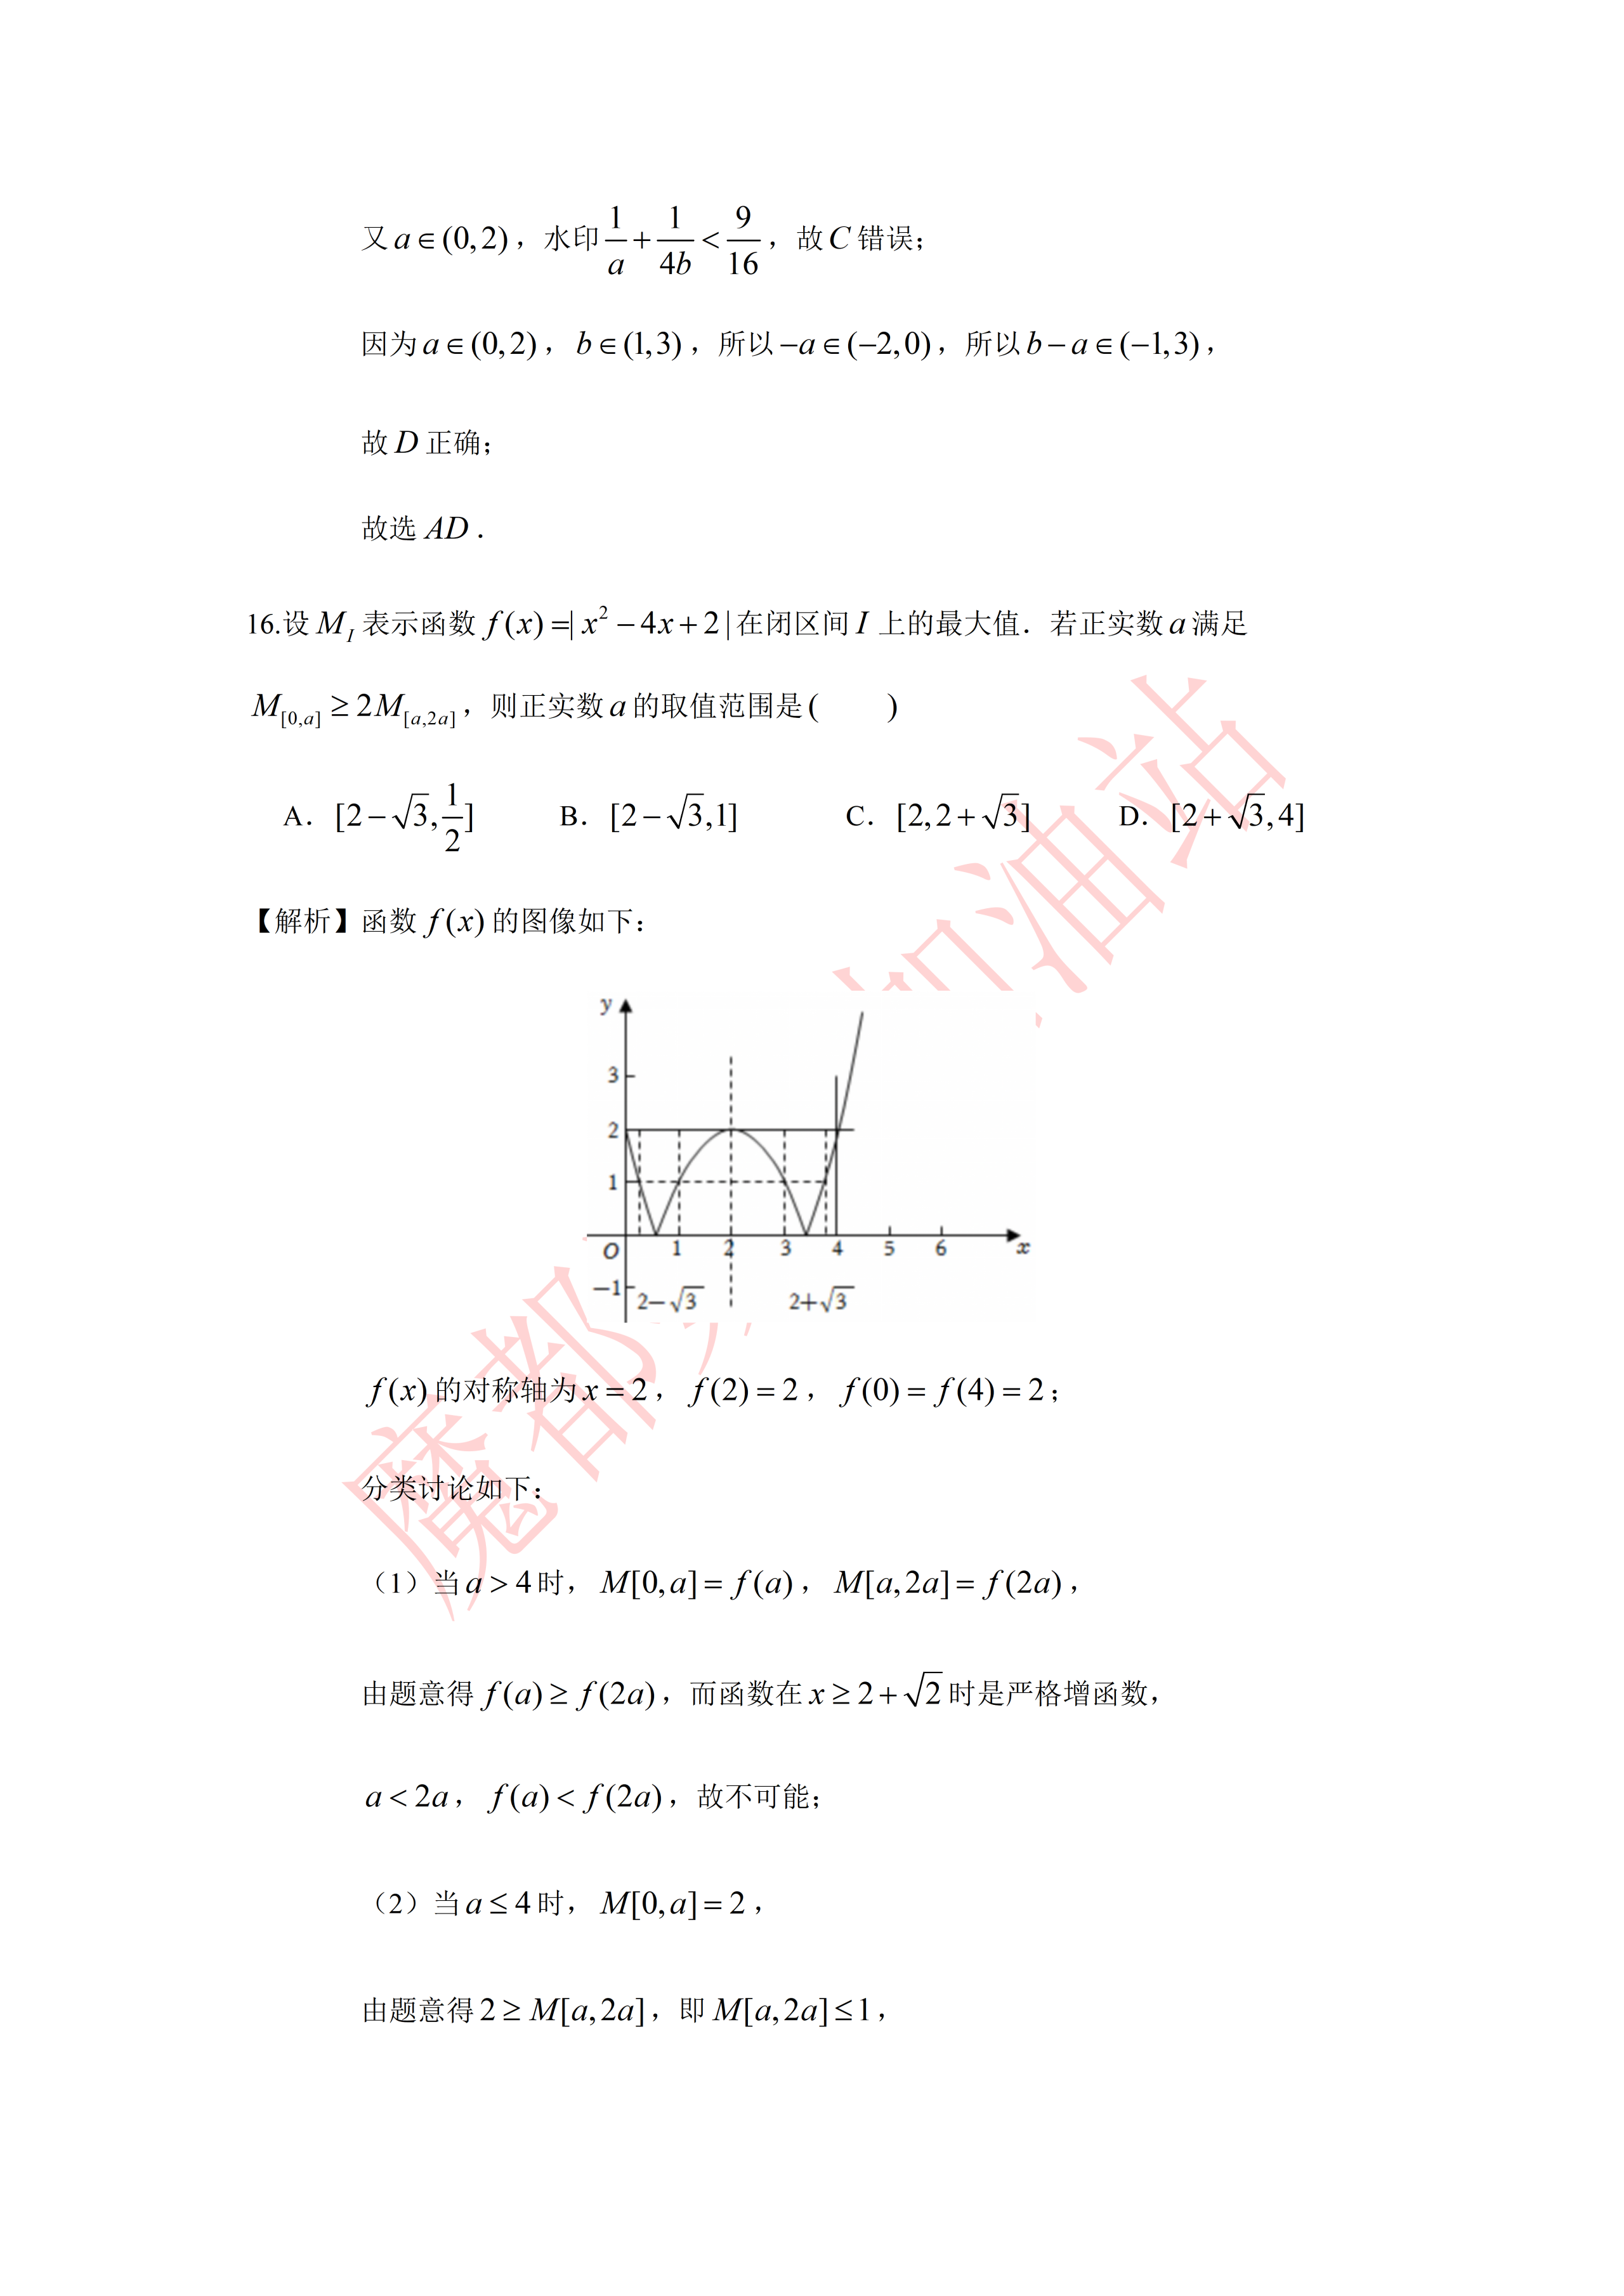
\includegraphics[width=.55\linewidth,trim=895bp 1535bp 915bp 1525bp,clip]{../原图/高一51_华师大二附中_国庆作业3/06.png}
\end{center}
\step{$f(x)$ 的对称轴为 $x=2$，$f(2)=2$，$f(0)=f(4)=2$；}
\step{分类讨论如下：}
\stepm{(1)}{当 $a>4$ 时，$M_{[0,a]}=f(a)$，$M_{[a,2a]}=f(2a)$，}
\step{由题意得 $f(a)\geqslant f(2a)$，而函数在 $x\geqslant2+\sqrt2$ 时是严格增函数，}
\step{$a<2a$，$f(a)<f(2a)$，故不可能；}
\stepm{(2)}{当 $a\leqslant4$ 时，$M_{[0,a]}=2$，}
\step{由题意得 $2\geqslant M_{[a,2a]}$，即 $M_{[a,2a]}\leqslant1$，}
\step{令 $f(x)=1$，解得 $x_1=2-\sqrt3$，$x_2=1$，$x_3=2+\sqrt3$，$x_4=3$，}
\step{则有 $a\geqslant2-\sqrt3$ 并且 $2a\leqslant1$，解得 $2-\sqrt3\leqslant a\leqslant\dfrac12$；}
\step{或者 $a\geqslant3$ 并且 $2a\leqslant2+\sqrt3$，无解；}
\step{故选 $A$.}
\solend

\fi

\end{enumerate}

\bigsec{三、解答题}

\begin{enumerate}
\setcounter{enumi}{16}

\item 已知 $M=\{x\mid2\leqslant x\leqslant5\}$，$N=\{x\mid a-1\leqslant x\leqslant2a+1\}$.
\begin{enumerate}[label=(\arabic*)]
\item 若 $M\subseteq N$，求实数 $a$ 的取值范围；
\item 若 $M\supseteq N$，求实数 $a$ 的取值范围.
\end{enumerate}

\ifanswer
\ans{（1）$[2,3]$；（2）$(-\infty,-2)$}
\fi

\ansspace[6]

\item 设集合 $A=\{x\mid|x+1|\leqslant3\}$，$B=\{x\mid0<x<3m\}$.
\begin{enumerate}[label=(\arabic*)]
\item 若 $A\cup B=A$，求实数 $m$ 的取值范围；
\item 设 $P=(\complement_R A)\cap B$，若 $\exists x\in\Z$ 且 $x\in P$，求实数 $m$ 的取值范围.
\end{enumerate}

\ifanswer
\solbegin
\stepm{(1)}{$A=\{x\mid|x+1|\leqslant3\}=\{x\mid-4\leqslant x\leqslant2\}$，且 $A\cup B=A$，所以 $B\subseteq A$.}
\step{若 $B=\varnothing$，此时 $0\geqslant3m$，解得 $m\leqslant0$；}
\step{若 $B\neq\varnothing$，此时 $0<3m$，且 $3m\leqslant2$，解得 $0<m\leqslant\dfrac23$；}
\step{则实数 $m$ 的取值范围是 $\left(-\infty,\dfrac23\right]$.}
\stepm{(2)}{因为 $\exists x\in\Z$ 且 $x\in P$，所以集合 $P$ 中至少存在一个整数.}
\step{$\complement_R A=\{x\mid x<-4\text{ 或 }x>2\}$，$B=\{x\mid0<x<3m\}$，}
\step{要使 $P=(\complement_R A)\cap B$ 中至少存在一个整数，则 $\begin{cases}3m>0\\3m>3\end{cases}$，解得 $m>1$，}
\step{则实数 $m$ 的取值范围是 $(1,+\infty)$.}
\solend

\fi

\ansspace[7]

\item 已知函数 $f(x)=x^2+(1-a)x-a(a\in\R)$.
\begin{enumerate}[label=(\arabic*)]
\item 解关于 $x$ 的不等式 $f(x)<0$；
\item 若 $\forall a\in[-1,1]$，$f(x)\geqslant0$ 恒成立，求实数 $x$ 的取值范围.
\end{enumerate}

\ifanswer
\solbegin
\stepm{(1)}{不等式 $x^2+(1-a)x-a<0$ 等价于 $(x-a)(x+1)<0$，}
\step{当 $a<-1$ 时，不等式的解集为 $(a,-1)$；}
\step{当 $a=-1$ 时，不等式的解集为 $\varnothing$；}
\step{当 $a>-1$ 时，不等式的解集为 $(-1,a)$.}
\stepm{(2)}{$x^2+(1-a)x-a=-a(x+1)+x^2+x$，}
\step{设 $g(a)=-a(x+1)+x^2+x$，$a\in[-1,1]$，}
\step{要使 $g(a)\geqslant0$ 在 $a\in[-1,1]$ 上恒成立，}
\step{只需 $\begin{cases}g(-1)\geqslant0\\g(1)\geqslant0\end{cases}$，即 $\begin{cases}x^2+2x+1\geqslant0\\x^2-1\geqslant0\end{cases}$，解得 $x\geqslant1$ 或 $x\leqslant-1$，}
\step{所以 $x$ 的取值范围为 $\{x\mid x\leqslant-1\text{ 或 }x\geqslant1\}$.}
\solend

\fi

\ansspace[7]

\item 若实数 $x$、$y$、$m$ 满足 $|x-m|>|y-m|$，则称 $x$ 比 $y$ 远离 $m$.
\begin{enumerate}[label=(\arabic*)]
\item 若 $2$ 比 $3x-4$ 远离 $1$，求 $x$ 的取值范围；
\item 设 $y=\dfrac{x+2}{x+1}$，其中 $x\in(0,\sqrt2)\cup(\sqrt2,+\infty)$，判断：$x$ 与 $y$ 哪一个更远离 $\sqrt2$？并说明理由.
\item 若 $x+y=2$，试问：$y$ 与 $x^2+y^2$ 哪一个更远离 $\dfrac12$？并说明理由.
\end{enumerate}

\ifanswer
\solbegin
\stepm{(1)}{由题意得 $|2-1|>|3x-4-1|$，所以 $|3x-5|<1$，解得 $\dfrac43<x<2$，}
\step{故 $x$ 的取值范围为 $\left(\dfrac43,2\right)$；}
\stepm{(2)}{$x$ 比 $y$ 更远离 $\sqrt2$，}
\step{理由如下：要证 $x$ 比 $y$ 更远离 $\sqrt2$，只要证 $|x-\sqrt2|>\left|\dfrac{x+2}{x+1}-\sqrt2\right|$，}
\step{即证 $|x-\sqrt2|>\left|\dfrac{(1-\sqrt2)(x-\sqrt2)}{x+1}\right|$，}
\step{因为 $x\in(0,\sqrt2)\cup(\sqrt2,+\infty)$，所以 $|x-\sqrt2|>0$，}
\step{所以只要证 $1>\dfrac{\sqrt2-1}{|x+1|}$，即证 $|x+1|>\sqrt2-1$，}
\step{因为 $x\in(0,\sqrt2)\cup(\sqrt2,+\infty)$，所以 $x+1\in(1,\sqrt2+1)\cup(\sqrt2+1,+\infty)$，}
\step{所以 $|x+1|>1>\sqrt2-1$，所以 $x$ 比 $y$ 更远离 $\sqrt2$；}
\stepm{(3)}{因为 $x^2+y^2\geqslant\dfrac{(x+y)^2}{2}=2$，当且仅当 $x=y=1$ 时等号成立，}
\step{所以 $\left|x^2+y^2-\dfrac12\right|=x^2+y^2-\dfrac12$，}
\step{从而 $\left|y-\dfrac12\right|-\left|x^2+y^2-\dfrac12\right|=\left|y-\dfrac12\right|-\left(x^2+y^2-\dfrac12\right)$，}
\step{①$y\geqslant\dfrac12$，$\left|y-\dfrac12\right|-\left|x^2+y^2-\dfrac12\right|=y-\dfrac12-\left(x^2+y^2-\dfrac12\right)=y-x^2-y^2$}
\step{$=y-(2-y)^2-y^2=-2y^2+5y-4=-2\left(y-\dfrac54\right)^2-\dfrac78<0$，}
\step{即 $\left|y-\dfrac12\right|<\left|x^2+y^2-\dfrac12\right|$；}
\step{②$y<\dfrac12$，}
\step{$\left|y-\dfrac12\right|-\left|x^2+y^2-\dfrac12\right|=\left(\dfrac12-y\right)-\left(x^2+y^2-\dfrac12\right)=-y-x^2-y^2+1$}
\step{$=-y-(2-y)^2-y^2+1=-2y^2+3y-3=-2\left(y-\dfrac34\right)^2-\dfrac{15}8<0$，}
\step{即 $\left|y-\dfrac12\right|<\left|x^2+y^2-\dfrac12\right|$；}
\step{综上，$\left|y-\dfrac12\right|<\left|x^2+y^2-\dfrac12\right|$，即 $x^2+y^2$ 比 $y$ 更远离 $\dfrac12$.}
\solend

\fi

\ansspace[9]

\item 对于非空有限整数集 $X$，$m\in\N^*$，定义 $X^m=\{x^m\mid x\in X\}$，对 $n\in\Z$，
$Y\oplus n=\{x+n\mid x\in Y\}$ 现有两个非空有限整数集 $A$、$B$，已知 $A\oplus1\subseteq B$ 且
$B^2\oplus(-4)\subseteq A$.
\begin{enumerate}[label=(\arabic*)]
\item 当 $A=\{-3,0\}$ 时求集合 $B$；
\item 证明：$A\subseteq\{-3,-2,0,1\}$；
\item 当 $A\oplus1=B$ 且 $B^2\oplus(-4)=A$ 时，任取 $a\in A$，$b\in B$ 构造函数
$f(x)=(x-a)(x-b)$ 问：当 $a$、$b$ 取何值时，$f(x)$ 的最小值最小？
\end{enumerate}

\ifanswer
\solbegin
\stepm{(1)}{因为 $A=\{-3,0\}$，$B^2\oplus(-4)\subseteq A$，}
\step{所以 $B^2\oplus(-4)$ 可能为 $\varnothing$、$\{-3\}$、$\{0\}$、$\{-3,0\}$，}
\step{当 $B^2\oplus(-4)=\varnothing$ 时 $B^2=\varnothing$，不满足非空，不合题意；}
\step{当 $B^2\oplus(-4)=\{-3\}$ 时 $B^2=\{1\}$，所以 $B=\{1,-1\}$、$\{1\}$、$\{-1\}$，}
\step{当 $B^2\oplus(-4)=\{0\}$ 时 $B^2=\{4\}$，所以 $B=\{2,-2\}$、$\{2\}$、$\{-2\}$，}
% 原卷如此，照录未改（此处作 $\{0,-3\}$，上一行同一集合作 $\{-3,0\}$）
\step{当 $B^2\oplus(-4)=\{0,-3\}$ 时 $B^2=\{4,1\}$，}
\step{所以 $B=\{1,2,-1,-2\}$、$\{2,-1,-2\}$、$\{2,1,-2\}$、$\{1,-1,-2\}$、$\{1,-1,2\}$、$\{1,2\}$、$\{-1,2\}$、$\{-1,-2\}$、$\{1,-2\}$，}
\step{又 $A\oplus1=\{-2,1\}\subseteq B$，得 $B$ 为 $\{1,-2\}$、$\{2,1,-2\}$、$\{1,-1,-2\}$、$\{1,2,-1,-2\}$.}
\stepm{(2)}{设 $x\in A$，因为 $A\oplus1\subseteq B$，所以 $x+1\in B$，}
\step{又 $B^2\oplus(-4)\subseteq A$，所以 $(x+1)^2-4\in A$，}
% 原卷如此，照录未改（此处及下文取 $x=2$ 处原卷均作 $(-4+1)^2-4=52-2a>0$）
\step{取 $x=-4$，则 $(-4+1)^2-4=52-2a>0$，$(5+1)^2-4=32\in A$，$\cdots$，}
\step{无限迭代，而 $A$ 为有限集，不合题意，舍去，即 $-4\notin A$；}
\step{取 $x=-3$，则 $(-3+1)^2-4=0\in A$，$(0+1)^2-4=-3\in A$，}
\step{得 $A$ 集合可为 $\{-3,0\}$；}
\step{取 $x=-2$，则 $(-2+1)^2-4=-3\in A$，$(-3+1)^2-4=0\in A$，}
\step{$(0+1)^2-4=-3\in A$，得 $A$ 集合可为 $\{-3,-2,0\}$；}
\step{取 $x=-1$，则 $(-1+1)^2-4=-4\in A$，又 $-4\notin A$，所以 $-1\notin A$，}
\step{取 $x=1$，则 $(1+1)^2-4=0\in A$，$(0+1)^2-4=-3\in A$，}
\step{$(-3+1)^2-4=0\in A$，得 $A$ 集合可为 $\{-3,0,1\}$，}
\step{取 $x=2$，则 $(2+1)^2-4=52-2a>0$，$(5+1)^2-4=32\in A$，$\cdots$，}
\step{无限迭代，而 $A$ 为有限集，不合题意，舍去，即 $2\notin A$，}
\step{同理当 $x<-4$ 或 $x>2$，且 $x\in\Z$ 时不符合 $A$ 为有限集，舍去；}
\step{故由上得 $A$ 集合可为 $\{-3,0\},\{-3,-2,0\},\{-3,0,1\},\{-3,-2,0,1\}$，}
\step{所以 $A\subseteq\{-3,-2,0,1\}$，}
\stepm{(3)}{当 $A\oplus1=B$ 且 $B^2\oplus(-4)=A$ 时，}
\step{设 $x\in B$，则 $x^2-4\in B^2\oplus(-4)=A$，}
% 原卷如此，照录未改（题设 $A=\{-3,0\}$，此处两个判别式取的是 $-2$ 与 $1$，均不属于 $A$）
\step{$x^2-4=-2$ 时 $x=\pm\sqrt2$，不为整数，不合题意；}
\step{$x^2-4=1$ 时 $x=\pm\sqrt5$，不为整数，不合题意；}
\step{所以 $A=\{-3,0\}$，又 $A\oplus1=B$，则 $B=\{-2,1\}$，}
\step{任取 $a\in A$，$b\in B$ 构造函数 $f(x)=(x-a)(x-b)$，}
\step{$f(x)=(x-a)(x-b)=x^2-(a+b)x+ab$}
\step{$=x^2-(a+b)x+\dfrac{(a+b)^2}{4}+ab-\dfrac{(a+b)^2}{4}$}
\step{$=\left[x-\dfrac{(a+b)}2\right]^2-\dfrac{(a-b)^2}{4}\geqslant-\dfrac{(a-b)^2}{4}$，所以 $f(x)_{min}=-\dfrac{(a-b)^2}{4}$，}
\step{又 $a\in A=\{-3,0\}$，$b\in B=\{-2,1\}$，所以 $a-b$ 的取值有 $-1,-4,2$，}
\step{所以 $f(x)_{min}=-\dfrac{(a-b)^2}{4}\geqslant-\dfrac{(-3-1)^2}{4}=-4$，}
\step{即当 $a=-3$，$b=1$ 时 $f(x)_{min}$ 的最小值为 $-4$.}
\solend

\fi

\ansspace*[12]

\end{enumerate}

\end{document}
"
% 紧凑版：xelatex "\def\iscompact{1}% 高一51_华师大二附中_国庆作业3.tex
%   —— 高一上数学“2026-2027 年华师大二附中高一上国庆作业 3”（讲评版）
% 试卷版：xelatex 高一51_华师大二附中_国庆作业3.tex
% 答案版：xelatex "\def\isanswer{1}\input{高一51_华师大二附中_国庆作业3.tex}"
% 紧凑版：xelatex "\def\iscompact{1}\input{高一51_华师大二附中_国庆作业3.tex}"
%
% 原始材料：微信公众号“魔都数学加油站”文章，作者破晓，连载“27学年高一51”；
% 原文标题“27学年高一51——2026-2027年上海市华师大二附中高一上国庆作业3”；
% 原文链接：https://mp.weixin.qq.com/s/95SLMEmPUT30s4U7wjr5Og。
% 该页面用 JS 渲染，未见明确发布日期；页面内时间戳约为 2026-10-05 21:37，本稿以该时刻记可得日期。
% 正文为 12 张 PNG 页：第 01、02、03、05、07、08、11 页 4762×6735，
% 第 04、06、09、10、12 页 2560×3620。按页序逐页读取，12 页全为试卷正文页
% （卷首标题在第 1 页页顶，卷末解答题止于第 12 页），无封面页、目录页或单独的页脚页。
% 卷面标题照原卷印作“2026-2027 年华师大二附中高一上国庆作业 3”（公众号标题中的“上海市”
% 卷面标题行没有，本稿照卷面），年份区间按全稿惯例排 en dash。
%
% 篇幅与题号：原卷自第 3 题起编号（第 1、2 题不在本卷内）。填空题 3—12（10 题）、
% 选择题 13—16（4 题）、解答题 17—21（5 题），共 19 题。本稿沿用原节与原题号，
% 只改排为全稿统一的大节样式（原卷小节标题为“一、填空题”“二、选择题”“三、解答题”）。
% 正文为讲评版：填空题 3—12 与选择题 13—16 只印【解析】（选择题的结论“故选 X”印在解析内），
% 按全稿口径这类题不另提 \ans{}；解答题第 17 题只印【答案】，故只给 \ans{}；
% 第 18—21 题只印【解析】。
%
% 副标题：原卷未印副标题。本稿按“知识模块”口径标作“集合与常用逻辑用语、不等式”：
% 19 题中集合与常用逻辑用语 8 题（3、4、6、10、13、17、18、21），
% 不等式（含函数最值、绝对值不等式）11 题（5、7、8、9、11、12、14、15、16、19、20），
% 两类均远超三分之一，故并标。口径同 高一46_交附闵行_国庆作业3、高一48_华师大二附中_周末作业2。
%
% 与原卷的排版差异：
%   ① 原卷每题下直接印【答案】或【解析】，本稿按全稿惯例将答案与解析置于答案版；
%   ② 原卷未印副标题，本稿按“知识模块”口径补出；
%   ③ 原卷填空横线按全稿惯例排为 \blankline[4.4em]；
%   ④ 原卷 $R$、$N$、$Z$ 均排斜体，本稿按全稿惯例改用花体 $\R$、$\N$、$\Z$（同 高一48）；
%   ⑤ 原卷第 12 题解析配图、第 13 题题干韦恩图都印在正文右侧的浮动位置，第 16 题解析配图
%      印在解析行间；本稿三图一律居中排，均自原图对应页裁切（trim），不另存图片文件；
%   ⑥ 原卷解答题未留作答空白，本稿按全稿惯例加 \ansspace；
%   ⑦ 原卷第 15 题解析第 7、8 两个印刷行是一串连等式的折行，本稿按“一条 \step ＝ 一个印刷行”
%      的口径分成两条 \step。
%
% 原卷笔误/存疑（均照录未改，正文对应处另有 % 注）：
%   ① 第 12 题解析末行作“区间长度之和为 $x_1-b+x_2-a=x_1-x_2-a-b=2+a+b-a-b=2$”，
%      按上一行 $x_1+x_2=2+a+b$，此处应为 $x_1+x_2$；原卷作 $x_1-x_2$。
%   ② 第 15 题解析“又 $a\in(0,2)$，”与 $\dfrac1a+\dfrac1{4b}<\dfrac9{16}$ 之间，
%      原卷正文夹印“水印”二字（系制版遗留字样，非试卷内容）。
%   ③ 第 21 题第 (2) 问解析两处（取 $x=-4$、取 $x=2$）作“$=52-2a>0$”，
%      与题设 $(x+1)^2-4$ 的取值（按 $x=-4$ 应为 $5$）不符，当系原卷算式遗留。
%   ④ 第 21 题第 (1) 问解析先写 $B^2\oplus(-4)$ 可能为 $\{-3,0\}$，后文又作 $\{0,-3\}$，
%      同一集合两种写法。
%   ⑤ 第 21 题第 (3) 问解析：题设 $B^2\oplus(-4)=A$ 且 $A=\{-3,0\}$ 时，由 $x^2-4\in A$
%      应得 $x^2-4=-3$ 或 $0$；原卷讨论的却是 $x^2-4=-2$ 与 $x^2-4=1$（两值均不属于 $A$），
%      与题设不合。
%
% 插图：3 张，均自原图裁切（无 \begin{tikzpicture} 重排）：
%   · 第 13 题题干韦恩图（原图第 04 页，图在题干与选项右侧）
%   · 第 12 题解析配图（原图第 04 页，图在解析右侧）
%   · 第 16 题解析配图（原图第 06 页，图在解析中间）
%
\documentclass[a4paper,11pt]{article}
\usepackage{common}

\begin{document}

\examtitlest[3]{2026--2027 年华师大二附中高一上国庆作业 3}{集合与常用逻辑用语、不等式}

\bigsec{一、填空题}

\begin{enumerate}
\setcounter{enumi}{2}

\item 若 $\{x\mid x<1\text{ 或 }x>4\}\cup\{x\mid m<x<2m+3\}=R$，则实数 $m$ 的取值范围为\blankline[4.4em].

\ifanswer
\solbegin
\step{因为 $\{x\mid x<1\text{ 或 }x>4\}\cup\{x\mid m<x<2m+3\}=R$，}
\step{所以 $\begin{cases}m<1\\2m+3>4\end{cases}$，解得 $\dfrac12<m<1$，所以 $m$ 的取值范围为 $\left(\dfrac12,1\right)$.}
\solend

\fi

\item 若“$x\leqslant5$”是“$x<a$”的必要不充分条件，则 $a$ 的取值范围是\blankline[4.4em].

\ifanswer
\solbegin
\step{若“$x\leqslant5$”是“$x<a$”的必要不充分条件，则 $\{x\mid x<a\}\subset\{x\mid x\leqslant5\}$，}
\step{所以 $a\leqslant5$.}
\solend

\fi

\item 实数 $x$、$y$ 满足 $x^2+2xy+4y^2=1$，则 $x+2y$ 的取值范围是\blankline[4.4em].

\ifanswer
\solbegin
\step{因为 $x^2+2xy+4y^2=(x+2y)^2-2xy=1$，}
\step{所以 $(x+2y)^2-1=x\cdot(2y)\leqslant\left(\dfrac{x+2y}{2}\right)^2$，当且仅当 $x=2y$ 时取等号，}
\step{解得 $-\dfrac{2\sqrt3}{3}\leqslant x+2y\leqslant\dfrac{2\sqrt3}{3}$，故 $x+2y$ 的取值范围是 $\left[-\dfrac{2\sqrt3}{3},\dfrac{2\sqrt3}{3}\right]$.}
\solend

\fi

\item 若命题 $p$：“$\exists x\in\R$，$5x^2-3x+m=0$”为假命题，则实数 $m$ 的取值范围为\blankline[4.4em].

\ifanswer
\solbegin
\step{若命题 $p$：$\exists x\in\R$，$5x^2-3x+m=0$ 为假命题，}
\step{则 $5x^2-3x+m=0$ 没有实数根，故 $\Delta=9-20m<0$，解得 $m>\dfrac9{20}$.}
\solend

\fi

\item 若当 $3\leqslant m\leqslant5$ 时，$mx^2-mx+m-9<0$ 有解，则实数 $x$ 的取值范围是\blankline[4.4em].

\ifanswer
\solbegin
\step{当 $3\leqslant m\leqslant5$ 时，$mx^2-mx+m-9<0$ 有解，}
\step{即 $(x^2-x+1)m-9<0$ 在 $m\in[3,5]$ 上有解，}
\step{因为 $x^2-x+1>0$，所以一次函数 $g(m)=(x^2-x+1)m-9$ 严格增，}
\step{所以只需 $g(3)=3x^2-3x-6<0$ 即可，}
\step{即 $x^2-x-2<0$，$(x-2)(x+1)<0$，解得 $-1<x<2$，}
\step{所以实数 $x$ 的取值范围是 $(-1,2)$.}
\solend

\fi

\item 已知不等式 $\dfrac{x}{x^2+4}\leqslant a$ 对任意的 $x\in[1,3]$ 恒成立，则实数 $a$ 的范围为\blankline[4.4em].

\ifanswer
\solbegin
\step{因为 $x\in[1,3]$，所以 $\dfrac{x}{x^2+4}=\dfrac{1}{x+\dfrac4x}\leqslant\dfrac{1}{2\sqrt{x\times\dfrac4x}}=\dfrac14$，}
\step{当且仅当 $x=\dfrac4x$ 时，即 $x=2$ 时取等号，即 $\dfrac{x}{x^2+4}$ 在 $x\in[1,3]$ 的最大值为 $\dfrac14$，}
\step{又由不等式 $\dfrac{x}{x^2+4}\leqslant a$ 对任意的 $x\in[1,3]$ 恒成立，所以 $a\geqslant\dfrac14$，}
\step{即实数 $a$ 的范围为 $\left[\dfrac14,+\infty\right)$.}
\solend

\fi

\item 甲、乙两人解关于 $x$ 的不等式 $x^2+bx+c<0$，甲写错了 $b$，正确计算后得到的解为 $\{x\mid1<x<2\}$；
乙写错了 $c$，正确计算后得到的解为 $\{x\mid-4<x<1\}$. 那么不等式 $\dfrac{bx+c}{x-2}<0$ 的解为\blankline[4.4em].

\ifanswer
\solbegin
\step{由 $x^2+bx+c<0$ 的解为 $\{x\mid1<x<2\}$，}
\step{则 $1$ 和 $2$ 是方程 $x^2+bx+c=0$ 的两个根，}
\step{甲写错了 $b$，但 $c$ 是正确的，所以 $c=1\times2=2$；}
\step{由 $x^2+bx+c<0$ 的解为 $\{x\mid-4<x<1\}$，}
\step{则 $-4$ 和 $1$ 是方程 $x^2+bx+c=0$ 的两个根，}
\step{乙写错了 $c$，但 $b$ 是正确的，所以 $-b=-4+1=-3$，即 $b=3$.}
\step{由 $\dfrac{bx+c}{x-2}<0$，得 $\dfrac{3x+2}{x-2}<0$，即 $(3x+2)(x-2)<0$，解得 $-\dfrac23<x<2$.}
\step{不等式 $\dfrac{bx+c}{x-2}<0$ 的解为 $\left\{x\mid-\dfrac23<x<2\right\}$.}
\solend

\fi

\item 已知 $\dfrac{1}{x-2}\geqslant1$ 是 $|x-a|<2$ 的充分非必要条件，则实数 $a$ 的取值范围是\blankline[4.4em].

\ifanswer
\solbegin
\step{由 $\dfrac{1}{x-2}\geqslant1$ 得 $\dfrac{3-x}{x-2}\geqslant0$，解得 $2<x\leqslant3$，由 $|x-a|<2$ 得 $a-2<x<a+2$，}
\step{因为 $\dfrac{1}{x-2}\geqslant1$ 是 $|x-a|<2$ 的充分非必要条件，}
\step{所以 $\{x\mid2<x\leqslant3\}\subset\{x\mid a-2<x<a+2\}$，所以 $\begin{cases}a-2\leqslant2\\a+2>3\end{cases}$，解得 $1<a\leqslant4$，}
\step{即实数 $a$ 的取值范围是 $(1,4]$.}
\solend

\fi

\item 设 $a>0$，$b>0$，若不等式 $a(a+1)^2+b(b+1)^2\geqslant\lambda ab$ 恒成立，则实数 $\lambda$ 的最大值为\blankline[4.4em].

\ifanswer
\solbegin
\step{$a(a+1)^2+b(b+1)^2\geqslant\lambda ab\Leftrightarrow\lambda\leqslant\dfrac{a(a+1)^2+b(b+1)^2}{ab}=\dfrac{(a+1)^2}{b}+\dfrac{(b+1)^2}{a}$，}
\step{从而原问题转化为求 $\dfrac{(a+1)^2}{b}+\dfrac{(b+1)^2}{a}$ 的最小值.}
\step{因为 $\dfrac{(a+1)^2}{b}+\dfrac{(b+1)^2}{a}=\dfrac{b^2+2b+1}{a}+\dfrac{a^2+2a+1}{b}$}
\step{$=\left(\dfrac{b^2}{a}+\dfrac{a^2}{b}\right)+2\left(\dfrac ba+\dfrac ab\right)+\left(\dfrac1a+\dfrac1b\right)\geqslant2\sqrt{\dfrac{b^2}{a}\cdot\dfrac{a^2}{b}}+2\times2\sqrt{\dfrac ba\cdot\dfrac ab}+2\sqrt{\dfrac1a\cdot\dfrac1b}$}
\step{$=2\sqrt{ab}+4+\dfrac{2}{\sqrt{ab}}\geqslant2\sqrt{2\sqrt{ab}\cdot\dfrac{2}{\sqrt{ab}}}+4=8$，以上均当且仅当 $a=b$ 时取等号，}
\step{所以 $\lambda\leqslant8$，即实数 $\lambda$ 的最大值为 $8$.}
\solend

\fi

\item 定义区间 $(a,d)$、$[a,d)$、$(a,d]$、$[a,d]$ 的长度为 $d-a$（$d>a$），已知 $a>b$，则满足
$\dfrac{1}{x-a}+\dfrac{1}{x-b}\geqslant1$ 的 $x$ 构成的区间的长度之和为\blankline[4.4em].

\ifanswer
\solbegin
\step{因为 $\dfrac{1}{x-a}+\dfrac{1}{x-b}\geqslant1$，所以 $\dfrac{2x-(a+b)}{(x-a)(x-b)}\geqslant1$，}
\step{即 $\dfrac{2x-(a+b)}{(x-a)(x-b)}-1\geqslant0$，则 $\dfrac{x^2-(2+a+b)x+ab+a+b}{(x-a)(x-b)}\leqslant0$，}
\step{设 $x^2-(2+a+b)x+ab+a+b=0$ 的根为 $x_1$ 和 $x_2$，}
\begin{center}
% 原卷该图印在解析右侧（原图第 04 页），本稿移作居中排，直接裁取原图，不另存图片文件。
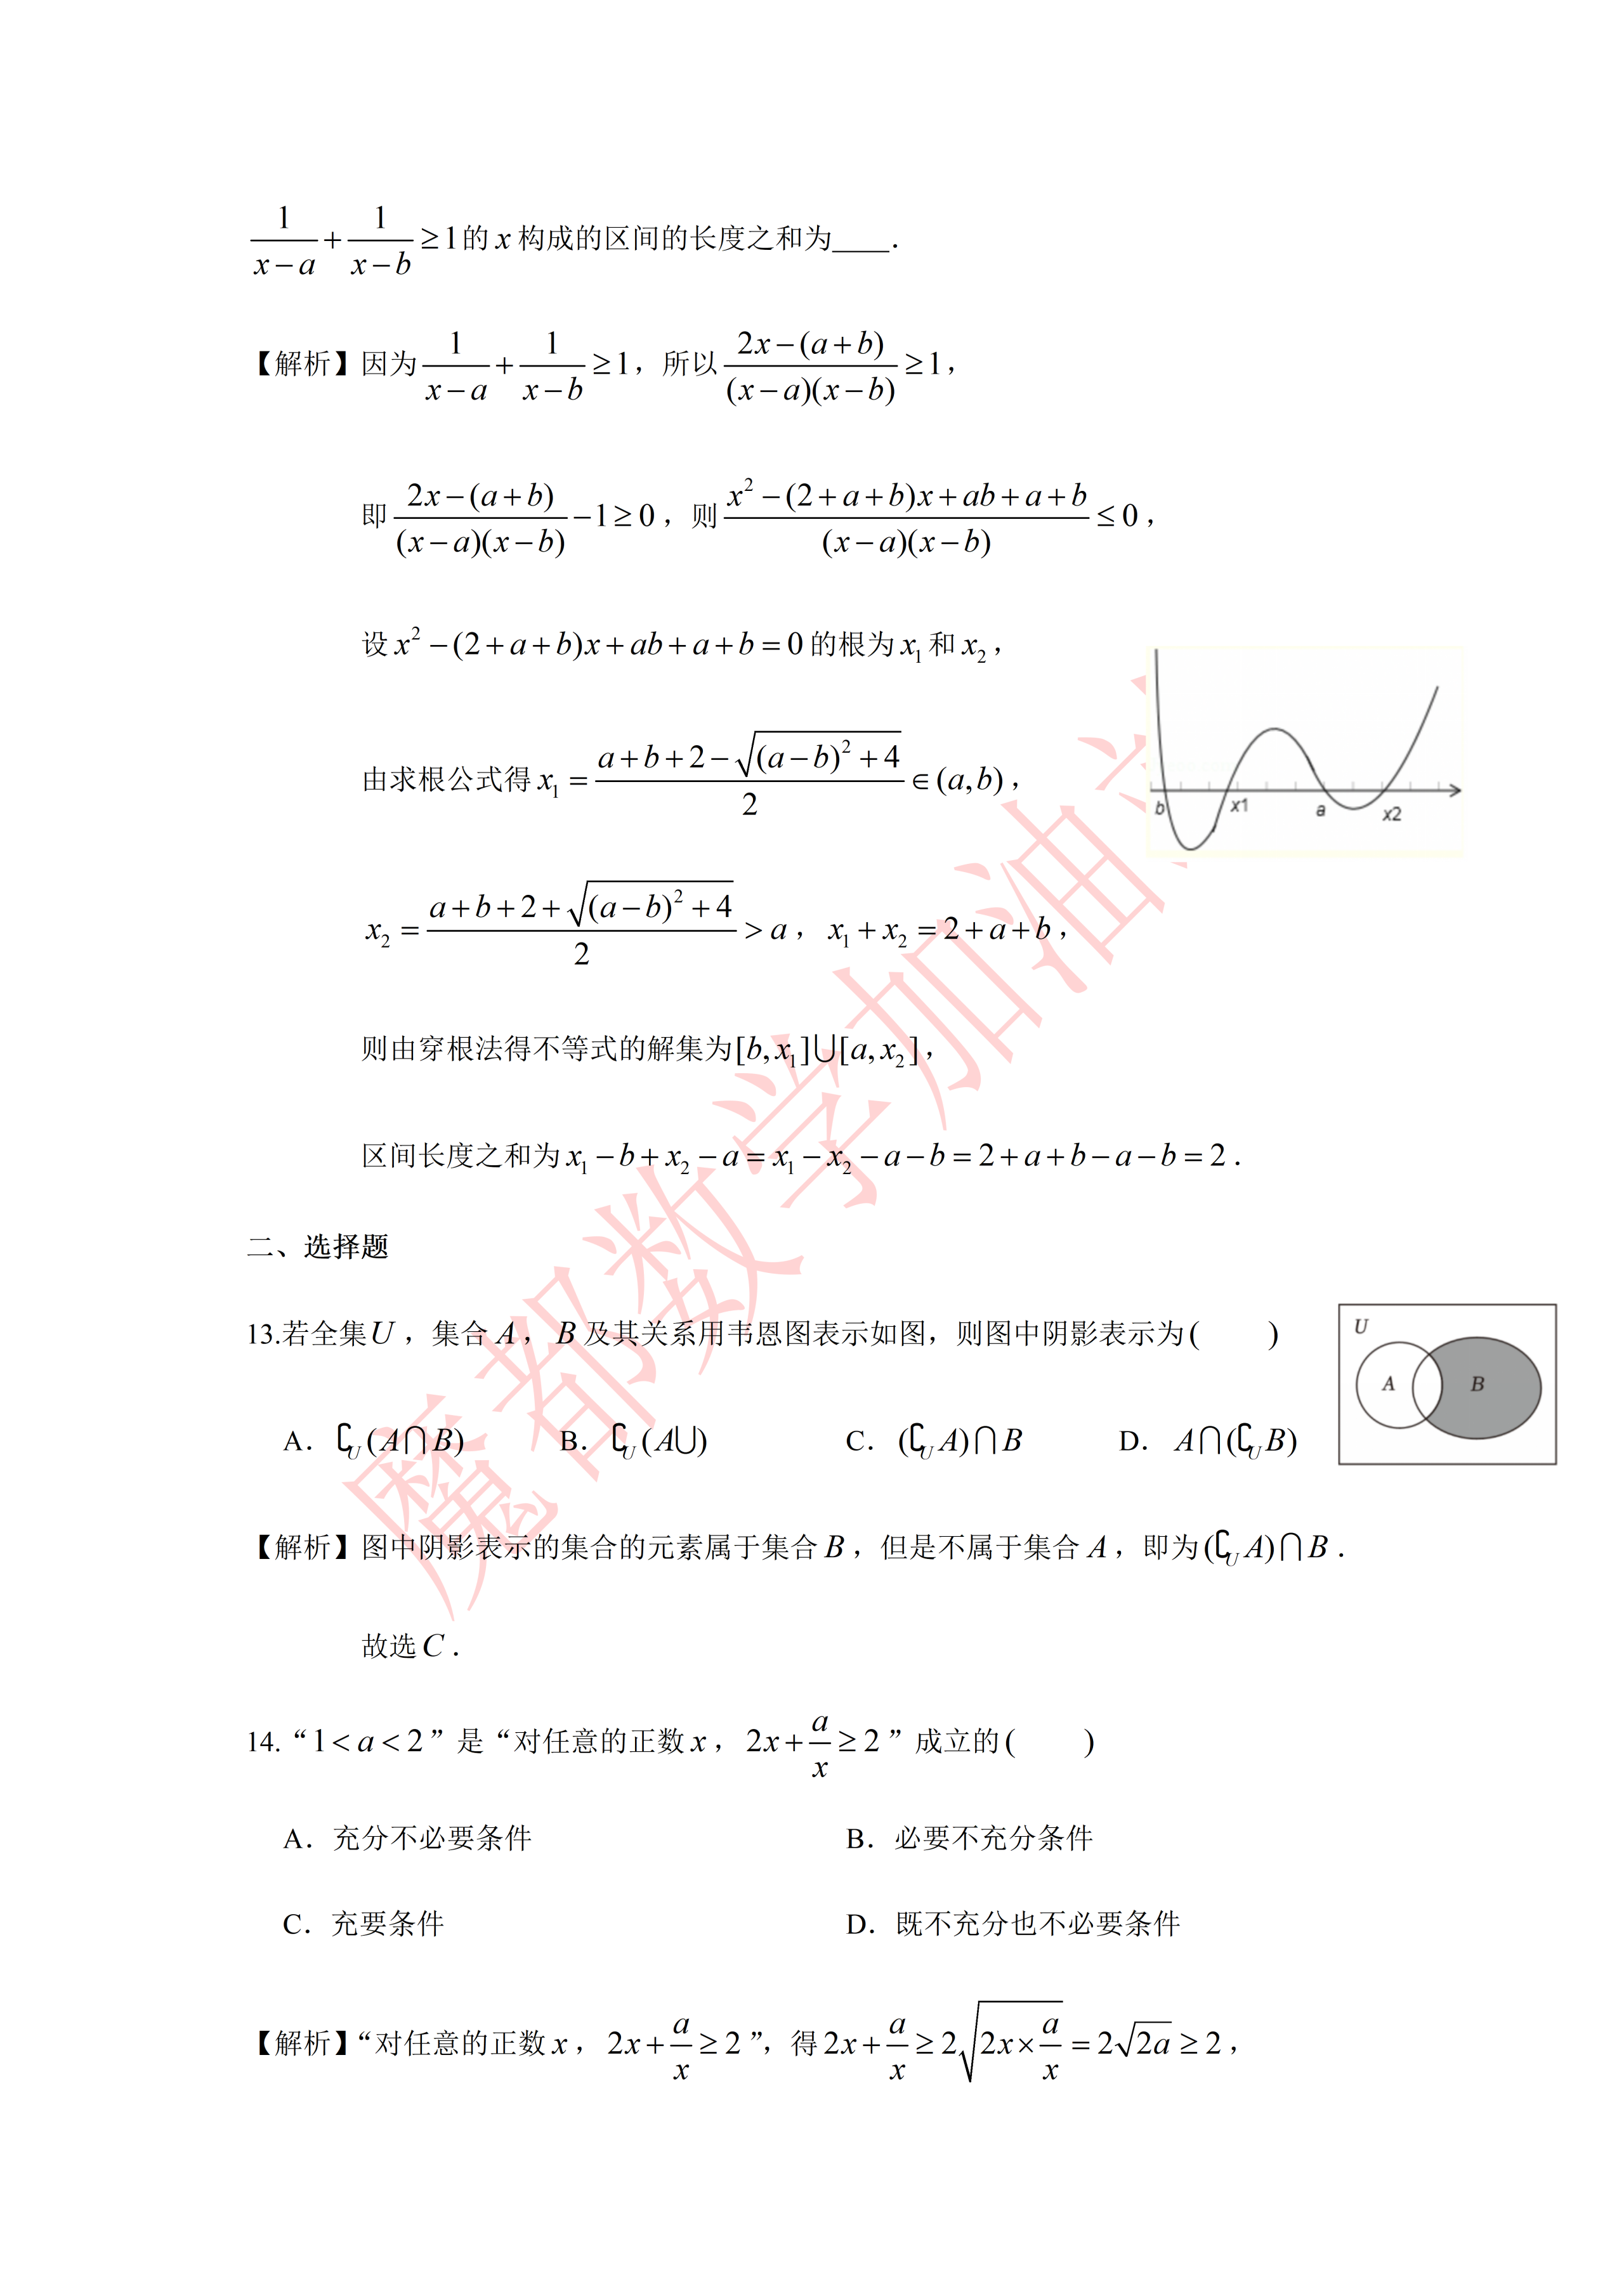
\includegraphics[width=.50\linewidth,trim=1786bp 2255bp 228bp 985bp,clip]{../原图/高一51_华师大二附中_国庆作业3/04.png}
\end{center}
\step{由求根公式得 $x_1=\dfrac{a+b+2-\sqrt{(a-b)^2+4}}{2}\in(a,b)$，}
\step{$x_2=\dfrac{a+b+2+\sqrt{(a-b)^2+4}}{2}>a$，$x_1+x_2=2+a+b$，}
\step{则由穿根法得不等式的解集为 $[b,x_1]\cup[a,x_2]$，}
% 原卷如此，照录未改（此处原卷作 $x_1-x_2$，按上一行 $x_1+x_2=2+a+b$ 当为 $x_1+x_2$）
\step{区间长度之和为 $x_1-b+x_2-a=x_1-x_2-a-b=2+a+b-a-b=2$.}
\solend

\fi

\end{enumerate}

\bigsec{二、选择题}

\begin{enumerate}
\setcounter{enumi}{12}

% 本题是“题干 + 图 + 选项”约 5.5cm 的一整块，图夹在题干与选项之间时 \keepwithprev 挡不住断点，
% 故按 高一30 第 13 题的成例在题前先量一次页高（守卫放在 \item 之前）。
\needvspace{6cm}
\item 若全集 $U$，集合 $A$、$B$ 及其关系用韦恩图表示如图，则图中阴影表示为\mbox{（\quad）}

\begin{center}
% 原卷该图印在题干与选项右侧（原图第 04 页），本稿移作居中排，直接裁取原图，不另存图片文件。
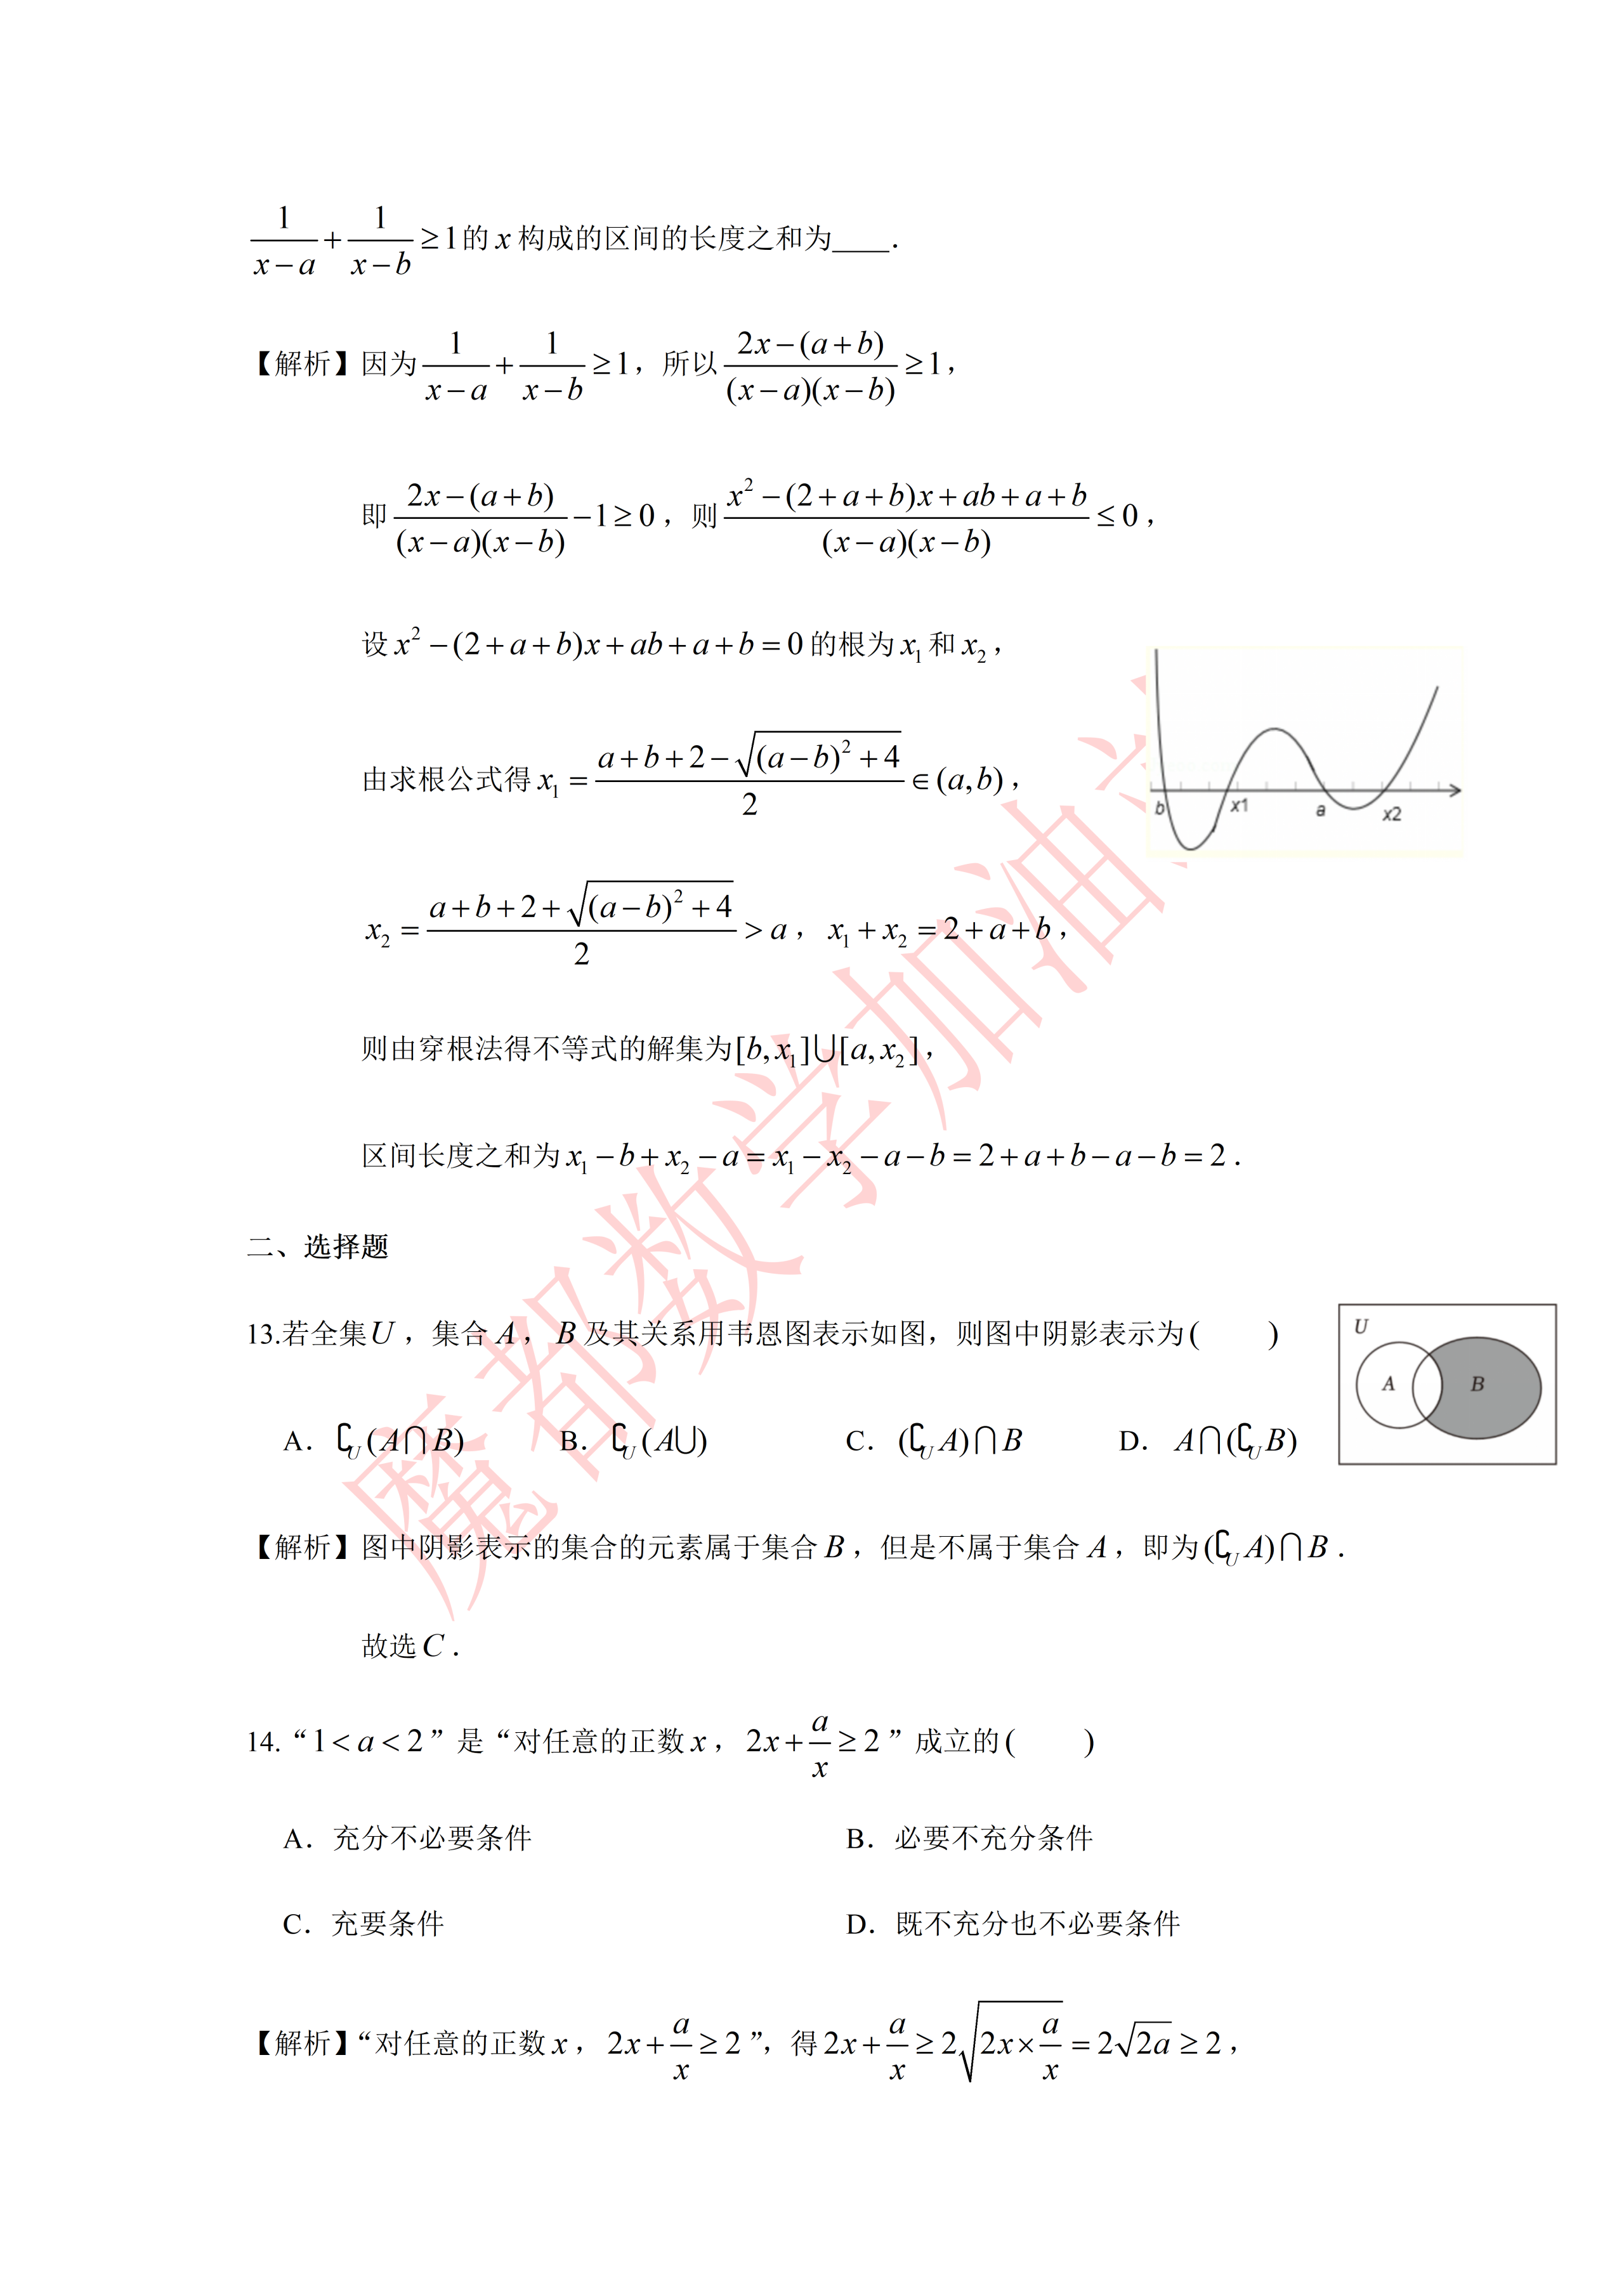
\includegraphics[width=.30\linewidth,trim=2105bp 1308bp 105bp 2050bp,clip]{../原图/高一51_华师大二附中_国庆作业3/04.png}
\end{center}

\keepwithprev
A. $\complement_U(A\cap B)$\qquad B. $\complement_U(A\cup B)$

C. $(\complement_U A)\cap B$\qquad D. $A\cap(\complement_U B)$

\ifanswer
\solbegin
\step{图中阴影表示的集合的元素属于集合 $B$，但是不属于集合 $A$，即为 $(\complement_U A)\cap B$.}
\step{故选 $C$.}
\solend

\fi

\item “$1<a<2$”是“对任意的正数 $x$，$2x+\dfrac ax\geqslant2$”成立的\mbox{（\quad）}

\keepwithprev
A. 充分不必要条件\qquad B. 必要不充分条件

C. 充要条件\qquad\qquad D. 既不充分也不必要条件

\ifanswer
\solbegin
\step{“对任意的正数 $x$，$2x+\dfrac ax\geqslant2$”，得 $2x+\dfrac ax\geqslant2\sqrt{2x\times\dfrac ax}=2\sqrt{2a}\geqslant2$，}
\step{所以 $\sqrt{2a}\geqslant1$，解得 $a\geqslant\dfrac12$，}
\step{若“$1<a<2$”得 $2x+\dfrac ax\geqslant2\sqrt{2x\times\dfrac ax}=2\sqrt{2a}>2\sqrt2>2$，}
\step{所以“$1<a<2$”$\Rightarrow$“对任意的正数 $x$，$2x+\dfrac ax\geqslant2$”，}
\step{所以“$1<a<2$”是“对任意的正数 $x$，$2x+\dfrac ax\geqslant2$”成立的充分不必要条件，}
\step{故选 $A$.}
\solend

\fi

\item 已知函数 $f(x)=2x-3$，$x\in(0,2)$，实数 $a$、$b$ 满足 $f(a)+f(b-1)=0$，则以下成立的有\mbox{（\quad）}

\keepwithprev
A. $a(b-1)$ 的最大值为 $\dfrac94$\qquad\qquad B. $b-\dfrac1a$ 的最大值为 $2$

C. $\dfrac1a+\dfrac1{4b}$ 的最小值为 $\dfrac9{16}$\qquad D. $-1<b-a<3$

\ifanswer
\solbegin
\step{因为函数 $f(x)=2x-3$，$x\in(0,2)$，实数 $a$、$b$ 满足 $f(a)+f(b-1)=0$，}
\step{所以 $2a-3+2(b-1)-3=0$，得 $a+b=4$，$a\in(0,2)$，$b\in(1,3)$，}
\step{所以 $a(b-1)=a(3-a)=-\left(a-\dfrac32\right)^2+\dfrac94$，$a\in(0,2)$，}
\step{所以 $0<a(b-1)\leqslant\dfrac94$，故选项 $A$ 正确；}
\step{$b-\dfrac1a=4-a-\dfrac1a=4-\left(a+\dfrac1a\right)\leqslant4-2=2$，}
\step{当且仅当 $a=1$，$b=3$ 时取等号，又 $b\in(1,3)$，故 $b-\dfrac1a<2$，故 $B$ 错误；}
\step{$\dfrac1a+\dfrac1{4b}=\dfrac14\left(\dfrac1a+\dfrac1{4b}\right)(a+b)=\dfrac14\left(1+\dfrac14+\dfrac ba+\dfrac a{4b}\right)=\dfrac5{16}+\dfrac14\left(\dfrac ba+\dfrac a{4b}\right)$}
\step{$\geqslant\dfrac5{16}+\dfrac14\cdot2\sqrt{\dfrac ba\cdot\dfrac a{4b}}=\dfrac9{16}$，当且仅当 $\dfrac ba=\dfrac a{4b}$，即 $a=2b=\dfrac83$ 时取等号，}
% 原卷如此，照录未改（“又 $a\in(0,2)$，”与下式之间原卷正文夹印“水印”二字）
\step{又 $a\in(0,2)$，水印 $\dfrac1a+\dfrac1{4b}<\dfrac9{16}$，故 $C$ 错误；}
\step{因为 $a\in(0,2)$，$b\in(1,3)$，所以 $-a\in(-2,0)$，所以 $b-a\in(-1,3)$，}
\step{故 $D$ 正确；}
\step{故选 $AD$.}
\solend

\fi

% 本题解析含图（“函数 f(x) 的图像如下”），图夹在解析行间，页末放不下会被拆开，
% 故在题前先量一次页高；上界取“题干 + 选项 + 图 + 首行解析”一块的高度。
\needvspace{6cm}
\item 设 $M_I$ 表示函数 $f(x)=|x^2-4x+2|$ 在闭区间 $I$ 上的最大值. 若正实数 $a$ 满足
$M_{[0,a]}\geqslant2M_{[a,2a]}$，则正实数 $a$ 的取值范围是\mbox{（\quad）}

\keepwithprev
A. $\left[2-\sqrt3,\dfrac12\right]$\qquad B. $[2-\sqrt3,1]$

C. $[2,2+\sqrt3]$\qquad\qquad D. $[2+\sqrt3,4]$

\ifanswer
\solbegin
\step{函数 $f(x)$ 的图像如下：}
\begin{center}
% 原卷该图印在解析行间（原图第 06 页），本稿直接裁取原图，不另存图片文件。
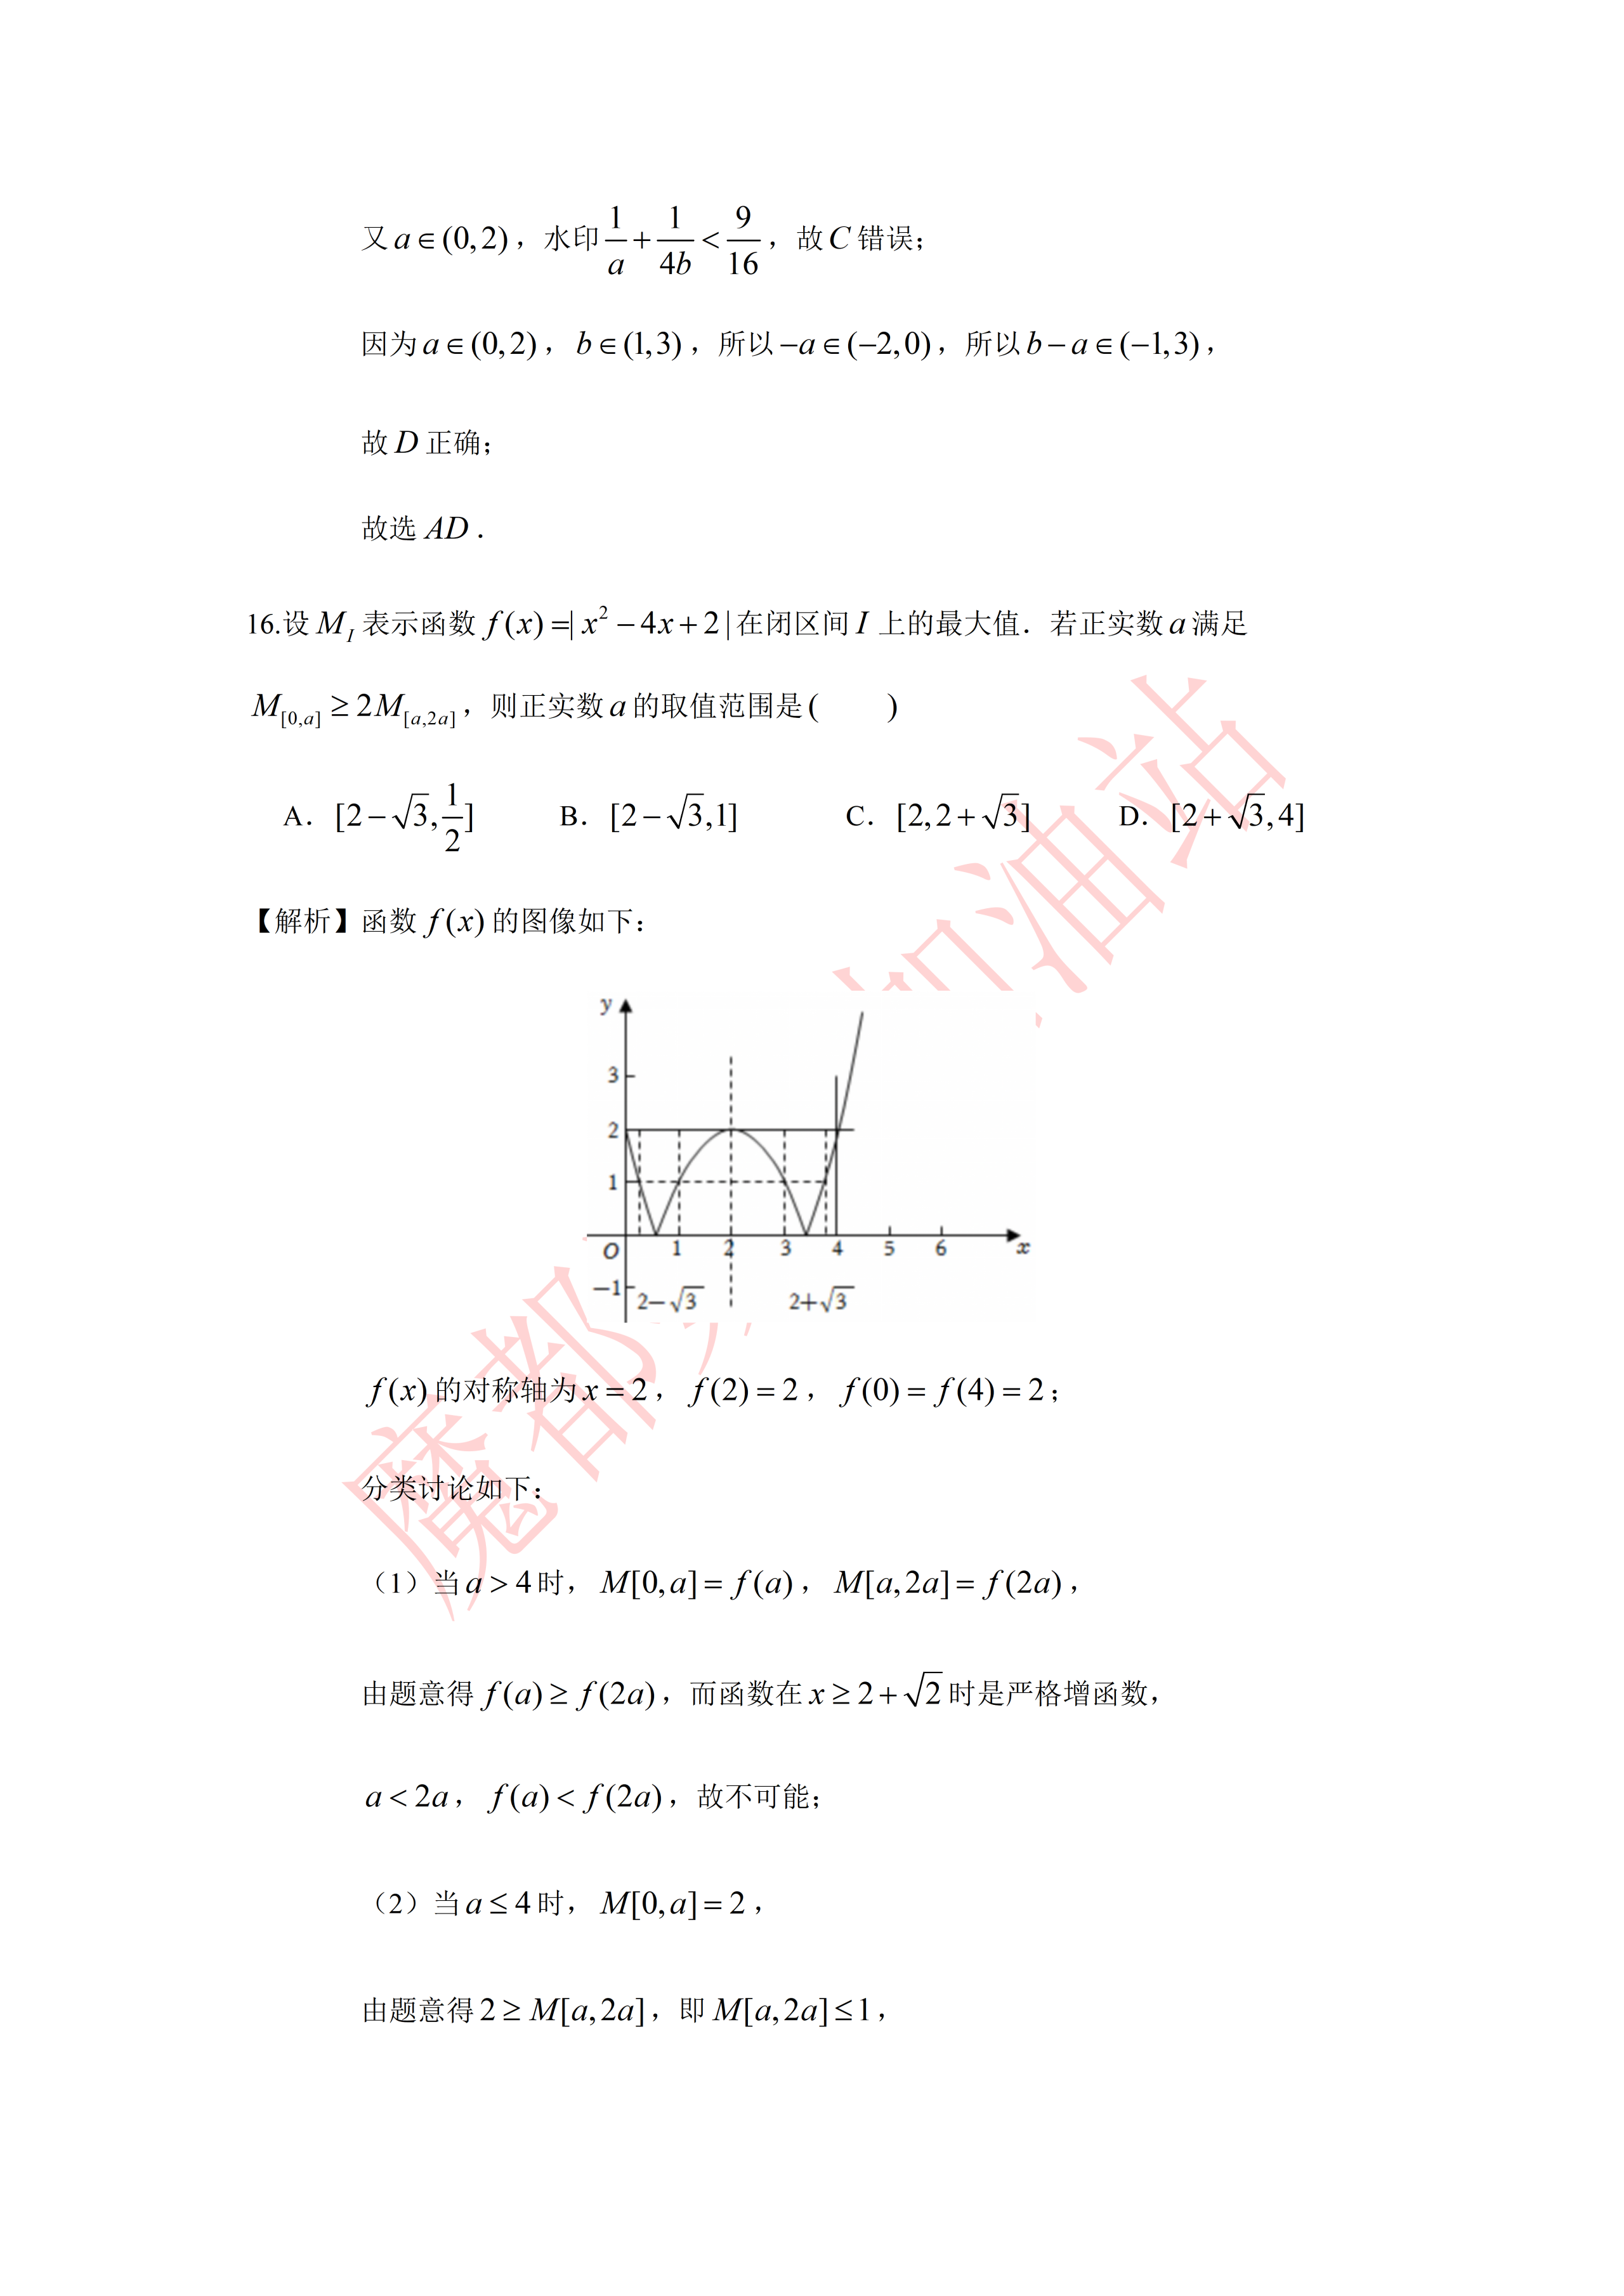
\includegraphics[width=.55\linewidth,trim=895bp 1535bp 915bp 1525bp,clip]{../原图/高一51_华师大二附中_国庆作业3/06.png}
\end{center}
\step{$f(x)$ 的对称轴为 $x=2$，$f(2)=2$，$f(0)=f(4)=2$；}
\step{分类讨论如下：}
\stepm{(1)}{当 $a>4$ 时，$M_{[0,a]}=f(a)$，$M_{[a,2a]}=f(2a)$，}
\step{由题意得 $f(a)\geqslant f(2a)$，而函数在 $x\geqslant2+\sqrt2$ 时是严格增函数，}
\step{$a<2a$，$f(a)<f(2a)$，故不可能；}
\stepm{(2)}{当 $a\leqslant4$ 时，$M_{[0,a]}=2$，}
\step{由题意得 $2\geqslant M_{[a,2a]}$，即 $M_{[a,2a]}\leqslant1$，}
\step{令 $f(x)=1$，解得 $x_1=2-\sqrt3$，$x_2=1$，$x_3=2+\sqrt3$，$x_4=3$，}
\step{则有 $a\geqslant2-\sqrt3$ 并且 $2a\leqslant1$，解得 $2-\sqrt3\leqslant a\leqslant\dfrac12$；}
\step{或者 $a\geqslant3$ 并且 $2a\leqslant2+\sqrt3$，无解；}
\step{故选 $A$.}
\solend

\fi

\end{enumerate}

\bigsec{三、解答题}

\begin{enumerate}
\setcounter{enumi}{16}

\item 已知 $M=\{x\mid2\leqslant x\leqslant5\}$，$N=\{x\mid a-1\leqslant x\leqslant2a+1\}$.
\begin{enumerate}[label=(\arabic*)]
\item 若 $M\subseteq N$，求实数 $a$ 的取值范围；
\item 若 $M\supseteq N$，求实数 $a$ 的取值范围.
\end{enumerate}

\ifanswer
\ans{（1）$[2,3]$；（2）$(-\infty,-2)$}
\fi

\ansspace[6]

\item 设集合 $A=\{x\mid|x+1|\leqslant3\}$，$B=\{x\mid0<x<3m\}$.
\begin{enumerate}[label=(\arabic*)]
\item 若 $A\cup B=A$，求实数 $m$ 的取值范围；
\item 设 $P=(\complement_R A)\cap B$，若 $\exists x\in\Z$ 且 $x\in P$，求实数 $m$ 的取值范围.
\end{enumerate}

\ifanswer
\solbegin
\stepm{(1)}{$A=\{x\mid|x+1|\leqslant3\}=\{x\mid-4\leqslant x\leqslant2\}$，且 $A\cup B=A$，所以 $B\subseteq A$.}
\step{若 $B=\varnothing$，此时 $0\geqslant3m$，解得 $m\leqslant0$；}
\step{若 $B\neq\varnothing$，此时 $0<3m$，且 $3m\leqslant2$，解得 $0<m\leqslant\dfrac23$；}
\step{则实数 $m$ 的取值范围是 $\left(-\infty,\dfrac23\right]$.}
\stepm{(2)}{因为 $\exists x\in\Z$ 且 $x\in P$，所以集合 $P$ 中至少存在一个整数.}
\step{$\complement_R A=\{x\mid x<-4\text{ 或 }x>2\}$，$B=\{x\mid0<x<3m\}$，}
\step{要使 $P=(\complement_R A)\cap B$ 中至少存在一个整数，则 $\begin{cases}3m>0\\3m>3\end{cases}$，解得 $m>1$，}
\step{则实数 $m$ 的取值范围是 $(1,+\infty)$.}
\solend

\fi

\ansspace[7]

\item 已知函数 $f(x)=x^2+(1-a)x-a(a\in\R)$.
\begin{enumerate}[label=(\arabic*)]
\item 解关于 $x$ 的不等式 $f(x)<0$；
\item 若 $\forall a\in[-1,1]$，$f(x)\geqslant0$ 恒成立，求实数 $x$ 的取值范围.
\end{enumerate}

\ifanswer
\solbegin
\stepm{(1)}{不等式 $x^2+(1-a)x-a<0$ 等价于 $(x-a)(x+1)<0$，}
\step{当 $a<-1$ 时，不等式的解集为 $(a,-1)$；}
\step{当 $a=-1$ 时，不等式的解集为 $\varnothing$；}
\step{当 $a>-1$ 时，不等式的解集为 $(-1,a)$.}
\stepm{(2)}{$x^2+(1-a)x-a=-a(x+1)+x^2+x$，}
\step{设 $g(a)=-a(x+1)+x^2+x$，$a\in[-1,1]$，}
\step{要使 $g(a)\geqslant0$ 在 $a\in[-1,1]$ 上恒成立，}
\step{只需 $\begin{cases}g(-1)\geqslant0\\g(1)\geqslant0\end{cases}$，即 $\begin{cases}x^2+2x+1\geqslant0\\x^2-1\geqslant0\end{cases}$，解得 $x\geqslant1$ 或 $x\leqslant-1$，}
\step{所以 $x$ 的取值范围为 $\{x\mid x\leqslant-1\text{ 或 }x\geqslant1\}$.}
\solend

\fi

\ansspace[7]

\item 若实数 $x$、$y$、$m$ 满足 $|x-m|>|y-m|$，则称 $x$ 比 $y$ 远离 $m$.
\begin{enumerate}[label=(\arabic*)]
\item 若 $2$ 比 $3x-4$ 远离 $1$，求 $x$ 的取值范围；
\item 设 $y=\dfrac{x+2}{x+1}$，其中 $x\in(0,\sqrt2)\cup(\sqrt2,+\infty)$，判断：$x$ 与 $y$ 哪一个更远离 $\sqrt2$？并说明理由.
\item 若 $x+y=2$，试问：$y$ 与 $x^2+y^2$ 哪一个更远离 $\dfrac12$？并说明理由.
\end{enumerate}

\ifanswer
\solbegin
\stepm{(1)}{由题意得 $|2-1|>|3x-4-1|$，所以 $|3x-5|<1$，解得 $\dfrac43<x<2$，}
\step{故 $x$ 的取值范围为 $\left(\dfrac43,2\right)$；}
\stepm{(2)}{$x$ 比 $y$ 更远离 $\sqrt2$，}
\step{理由如下：要证 $x$ 比 $y$ 更远离 $\sqrt2$，只要证 $|x-\sqrt2|>\left|\dfrac{x+2}{x+1}-\sqrt2\right|$，}
\step{即证 $|x-\sqrt2|>\left|\dfrac{(1-\sqrt2)(x-\sqrt2)}{x+1}\right|$，}
\step{因为 $x\in(0,\sqrt2)\cup(\sqrt2,+\infty)$，所以 $|x-\sqrt2|>0$，}
\step{所以只要证 $1>\dfrac{\sqrt2-1}{|x+1|}$，即证 $|x+1|>\sqrt2-1$，}
\step{因为 $x\in(0,\sqrt2)\cup(\sqrt2,+\infty)$，所以 $x+1\in(1,\sqrt2+1)\cup(\sqrt2+1,+\infty)$，}
\step{所以 $|x+1|>1>\sqrt2-1$，所以 $x$ 比 $y$ 更远离 $\sqrt2$；}
\stepm{(3)}{因为 $x^2+y^2\geqslant\dfrac{(x+y)^2}{2}=2$，当且仅当 $x=y=1$ 时等号成立，}
\step{所以 $\left|x^2+y^2-\dfrac12\right|=x^2+y^2-\dfrac12$，}
\step{从而 $\left|y-\dfrac12\right|-\left|x^2+y^2-\dfrac12\right|=\left|y-\dfrac12\right|-\left(x^2+y^2-\dfrac12\right)$，}
\step{①$y\geqslant\dfrac12$，$\left|y-\dfrac12\right|-\left|x^2+y^2-\dfrac12\right|=y-\dfrac12-\left(x^2+y^2-\dfrac12\right)=y-x^2-y^2$}
\step{$=y-(2-y)^2-y^2=-2y^2+5y-4=-2\left(y-\dfrac54\right)^2-\dfrac78<0$，}
\step{即 $\left|y-\dfrac12\right|<\left|x^2+y^2-\dfrac12\right|$；}
\step{②$y<\dfrac12$，}
\step{$\left|y-\dfrac12\right|-\left|x^2+y^2-\dfrac12\right|=\left(\dfrac12-y\right)-\left(x^2+y^2-\dfrac12\right)=-y-x^2-y^2+1$}
\step{$=-y-(2-y)^2-y^2+1=-2y^2+3y-3=-2\left(y-\dfrac34\right)^2-\dfrac{15}8<0$，}
\step{即 $\left|y-\dfrac12\right|<\left|x^2+y^2-\dfrac12\right|$；}
\step{综上，$\left|y-\dfrac12\right|<\left|x^2+y^2-\dfrac12\right|$，即 $x^2+y^2$ 比 $y$ 更远离 $\dfrac12$.}
\solend

\fi

\ansspace[9]

\item 对于非空有限整数集 $X$，$m\in\N^*$，定义 $X^m=\{x^m\mid x\in X\}$，对 $n\in\Z$，
$Y\oplus n=\{x+n\mid x\in Y\}$ 现有两个非空有限整数集 $A$、$B$，已知 $A\oplus1\subseteq B$ 且
$B^2\oplus(-4)\subseteq A$.
\begin{enumerate}[label=(\arabic*)]
\item 当 $A=\{-3,0\}$ 时求集合 $B$；
\item 证明：$A\subseteq\{-3,-2,0,1\}$；
\item 当 $A\oplus1=B$ 且 $B^2\oplus(-4)=A$ 时，任取 $a\in A$，$b\in B$ 构造函数
$f(x)=(x-a)(x-b)$ 问：当 $a$、$b$ 取何值时，$f(x)$ 的最小值最小？
\end{enumerate}

\ifanswer
\solbegin
\stepm{(1)}{因为 $A=\{-3,0\}$，$B^2\oplus(-4)\subseteq A$，}
\step{所以 $B^2\oplus(-4)$ 可能为 $\varnothing$、$\{-3\}$、$\{0\}$、$\{-3,0\}$，}
\step{当 $B^2\oplus(-4)=\varnothing$ 时 $B^2=\varnothing$，不满足非空，不合题意；}
\step{当 $B^2\oplus(-4)=\{-3\}$ 时 $B^2=\{1\}$，所以 $B=\{1,-1\}$、$\{1\}$、$\{-1\}$，}
\step{当 $B^2\oplus(-4)=\{0\}$ 时 $B^2=\{4\}$，所以 $B=\{2,-2\}$、$\{2\}$、$\{-2\}$，}
% 原卷如此，照录未改（此处作 $\{0,-3\}$，上一行同一集合作 $\{-3,0\}$）
\step{当 $B^2\oplus(-4)=\{0,-3\}$ 时 $B^2=\{4,1\}$，}
\step{所以 $B=\{1,2,-1,-2\}$、$\{2,-1,-2\}$、$\{2,1,-2\}$、$\{1,-1,-2\}$、$\{1,-1,2\}$、$\{1,2\}$、$\{-1,2\}$、$\{-1,-2\}$、$\{1,-2\}$，}
\step{又 $A\oplus1=\{-2,1\}\subseteq B$，得 $B$ 为 $\{1,-2\}$、$\{2,1,-2\}$、$\{1,-1,-2\}$、$\{1,2,-1,-2\}$.}
\stepm{(2)}{设 $x\in A$，因为 $A\oplus1\subseteq B$，所以 $x+1\in B$，}
\step{又 $B^2\oplus(-4)\subseteq A$，所以 $(x+1)^2-4\in A$，}
% 原卷如此，照录未改（此处及下文取 $x=2$ 处原卷均作 $(-4+1)^2-4=52-2a>0$）
\step{取 $x=-4$，则 $(-4+1)^2-4=52-2a>0$，$(5+1)^2-4=32\in A$，$\cdots$，}
\step{无限迭代，而 $A$ 为有限集，不合题意，舍去，即 $-4\notin A$；}
\step{取 $x=-3$，则 $(-3+1)^2-4=0\in A$，$(0+1)^2-4=-3\in A$，}
\step{得 $A$ 集合可为 $\{-3,0\}$；}
\step{取 $x=-2$，则 $(-2+1)^2-4=-3\in A$，$(-3+1)^2-4=0\in A$，}
\step{$(0+1)^2-4=-3\in A$，得 $A$ 集合可为 $\{-3,-2,0\}$；}
\step{取 $x=-1$，则 $(-1+1)^2-4=-4\in A$，又 $-4\notin A$，所以 $-1\notin A$，}
\step{取 $x=1$，则 $(1+1)^2-4=0\in A$，$(0+1)^2-4=-3\in A$，}
\step{$(-3+1)^2-4=0\in A$，得 $A$ 集合可为 $\{-3,0,1\}$，}
\step{取 $x=2$，则 $(2+1)^2-4=52-2a>0$，$(5+1)^2-4=32\in A$，$\cdots$，}
\step{无限迭代，而 $A$ 为有限集，不合题意，舍去，即 $2\notin A$，}
\step{同理当 $x<-4$ 或 $x>2$，且 $x\in\Z$ 时不符合 $A$ 为有限集，舍去；}
\step{故由上得 $A$ 集合可为 $\{-3,0\},\{-3,-2,0\},\{-3,0,1\},\{-3,-2,0,1\}$，}
\step{所以 $A\subseteq\{-3,-2,0,1\}$，}
\stepm{(3)}{当 $A\oplus1=B$ 且 $B^2\oplus(-4)=A$ 时，}
\step{设 $x\in B$，则 $x^2-4\in B^2\oplus(-4)=A$，}
% 原卷如此，照录未改（题设 $A=\{-3,0\}$，此处两个判别式取的是 $-2$ 与 $1$，均不属于 $A$）
\step{$x^2-4=-2$ 时 $x=\pm\sqrt2$，不为整数，不合题意；}
\step{$x^2-4=1$ 时 $x=\pm\sqrt5$，不为整数，不合题意；}
\step{所以 $A=\{-3,0\}$，又 $A\oplus1=B$，则 $B=\{-2,1\}$，}
\step{任取 $a\in A$，$b\in B$ 构造函数 $f(x)=(x-a)(x-b)$，}
\step{$f(x)=(x-a)(x-b)=x^2-(a+b)x+ab$}
\step{$=x^2-(a+b)x+\dfrac{(a+b)^2}{4}+ab-\dfrac{(a+b)^2}{4}$}
\step{$=\left[x-\dfrac{(a+b)}2\right]^2-\dfrac{(a-b)^2}{4}\geqslant-\dfrac{(a-b)^2}{4}$，所以 $f(x)_{min}=-\dfrac{(a-b)^2}{4}$，}
\step{又 $a\in A=\{-3,0\}$，$b\in B=\{-2,1\}$，所以 $a-b$ 的取值有 $-1,-4,2$，}
\step{所以 $f(x)_{min}=-\dfrac{(a-b)^2}{4}\geqslant-\dfrac{(-3-1)^2}{4}=-4$，}
\step{即当 $a=-3$，$b=1$ 时 $f(x)_{min}$ 的最小值为 $-4$.}
\solend

\fi

\ansspace*[12]

\end{enumerate}

\end{document}
"
%
% 原始材料：微信公众号“魔都数学加油站”文章，作者破晓，连载“27学年高一51”；
% 原文标题“27学年高一51——2026-2027年上海市华师大二附中高一上国庆作业3”；
% 原文链接：https://mp.weixin.qq.com/s/95SLMEmPUT30s4U7wjr5Og。
% 该页面用 JS 渲染，未见明确发布日期；页面内时间戳约为 2026-10-05 21:37，本稿以该时刻记可得日期。
% 正文为 12 张 PNG 页：第 01、02、03、05、07、08、11 页 4762×6735，
% 第 04、06、09、10、12 页 2560×3620。按页序逐页读取，12 页全为试卷正文页
% （卷首标题在第 1 页页顶，卷末解答题止于第 12 页），无封面页、目录页或单独的页脚页。
% 卷面标题照原卷印作“2026-2027 年华师大二附中高一上国庆作业 3”（公众号标题中的“上海市”
% 卷面标题行没有，本稿照卷面），年份区间按全稿惯例排 en dash。
%
% 篇幅与题号：原卷自第 3 题起编号（第 1、2 题不在本卷内）。填空题 3—12（10 题）、
% 选择题 13—16（4 题）、解答题 17—21（5 题），共 19 题。本稿沿用原节与原题号，
% 只改排为全稿统一的大节样式（原卷小节标题为“一、填空题”“二、选择题”“三、解答题”）。
% 正文为讲评版：填空题 3—12 与选择题 13—16 只印【解析】（选择题的结论“故选 X”印在解析内），
% 按全稿口径这类题不另提 \ans{}；解答题第 17 题只印【答案】，故只给 \ans{}；
% 第 18—21 题只印【解析】。
%
% 副标题：原卷未印副标题。本稿按“知识模块”口径标作“集合与常用逻辑用语、不等式”：
% 19 题中集合与常用逻辑用语 8 题（3、4、6、10、13、17、18、21），
% 不等式（含函数最值、绝对值不等式）11 题（5、7、8、9、11、12、14、15、16、19、20），
% 两类均远超三分之一，故并标。口径同 高一46_交附闵行_国庆作业3、高一48_华师大二附中_周末作业2。
%
% 与原卷的排版差异：
%   ① 原卷每题下直接印【答案】或【解析】，本稿按全稿惯例将答案与解析置于答案版；
%   ② 原卷未印副标题，本稿按“知识模块”口径补出；
%   ③ 原卷填空横线按全稿惯例排为 \blankline[4.4em]；
%   ④ 原卷 $R$、$N$、$Z$ 均排斜体，本稿按全稿惯例改用花体 $\R$、$\N$、$\Z$（同 高一48）；
%   ⑤ 原卷第 12 题解析配图、第 13 题题干韦恩图都印在正文右侧的浮动位置，第 16 题解析配图
%      印在解析行间；本稿三图一律居中排，均自原图对应页裁切（trim），不另存图片文件；
%   ⑥ 原卷解答题未留作答空白，本稿按全稿惯例加 \ansspace；
%   ⑦ 原卷第 15 题解析第 7、8 两个印刷行是一串连等式的折行，本稿按“一条 \step ＝ 一个印刷行”
%      的口径分成两条 \step。
%
% 原卷笔误/存疑（均照录未改，正文对应处另有 % 注）：
%   ① 第 12 题解析末行作“区间长度之和为 $x_1-b+x_2-a=x_1-x_2-a-b=2+a+b-a-b=2$”，
%      按上一行 $x_1+x_2=2+a+b$，此处应为 $x_1+x_2$；原卷作 $x_1-x_2$。
%   ② 第 15 题解析“又 $a\in(0,2)$，”与 $\dfrac1a+\dfrac1{4b}<\dfrac9{16}$ 之间，
%      原卷正文夹印“水印”二字（系制版遗留字样，非试卷内容）。
%   ③ 第 21 题第 (2) 问解析两处（取 $x=-4$、取 $x=2$）作“$=52-2a>0$”，
%      与题设 $(x+1)^2-4$ 的取值（按 $x=-4$ 应为 $5$）不符，当系原卷算式遗留。
%   ④ 第 21 题第 (1) 问解析先写 $B^2\oplus(-4)$ 可能为 $\{-3,0\}$，后文又作 $\{0,-3\}$，
%      同一集合两种写法。
%   ⑤ 第 21 题第 (3) 问解析：题设 $B^2\oplus(-4)=A$ 且 $A=\{-3,0\}$ 时，由 $x^2-4\in A$
%      应得 $x^2-4=-3$ 或 $0$；原卷讨论的却是 $x^2-4=-2$ 与 $x^2-4=1$（两值均不属于 $A$），
%      与题设不合。
%
% 插图：3 张，均自原图裁切（无 \begin{tikzpicture} 重排）：
%   · 第 13 题题干韦恩图（原图第 04 页，图在题干与选项右侧）
%   · 第 12 题解析配图（原图第 04 页，图在解析右侧）
%   · 第 16 题解析配图（原图第 06 页，图在解析中间）
%
\documentclass[a4paper,11pt]{article}
\usepackage{common}

\begin{document}

\examtitlest[3]{2026--2027 年华师大二附中高一上国庆作业 3}{集合与常用逻辑用语、不等式}

\bigsec{一、填空题}

\begin{enumerate}
\setcounter{enumi}{2}

\item 若 $\{x\mid x<1\text{ 或 }x>4\}\cup\{x\mid m<x<2m+3\}=R$，则实数 $m$ 的取值范围为\blankline[4.4em].

\ifanswer
\solbegin
\step{因为 $\{x\mid x<1\text{ 或 }x>4\}\cup\{x\mid m<x<2m+3\}=R$，}
\step{所以 $\begin{cases}m<1\\2m+3>4\end{cases}$，解得 $\dfrac12<m<1$，所以 $m$ 的取值范围为 $\left(\dfrac12,1\right)$.}
\solend

\fi

\item 若“$x\leqslant5$”是“$x<a$”的必要不充分条件，则 $a$ 的取值范围是\blankline[4.4em].

\ifanswer
\solbegin
\step{若“$x\leqslant5$”是“$x<a$”的必要不充分条件，则 $\{x\mid x<a\}\subset\{x\mid x\leqslant5\}$，}
\step{所以 $a\leqslant5$.}
\solend

\fi

\item 实数 $x$、$y$ 满足 $x^2+2xy+4y^2=1$，则 $x+2y$ 的取值范围是\blankline[4.4em].

\ifanswer
\solbegin
\step{因为 $x^2+2xy+4y^2=(x+2y)^2-2xy=1$，}
\step{所以 $(x+2y)^2-1=x\cdot(2y)\leqslant\left(\dfrac{x+2y}{2}\right)^2$，当且仅当 $x=2y$ 时取等号，}
\step{解得 $-\dfrac{2\sqrt3}{3}\leqslant x+2y\leqslant\dfrac{2\sqrt3}{3}$，故 $x+2y$ 的取值范围是 $\left[-\dfrac{2\sqrt3}{3},\dfrac{2\sqrt3}{3}\right]$.}
\solend

\fi

\item 若命题 $p$：“$\exists x\in\R$，$5x^2-3x+m=0$”为假命题，则实数 $m$ 的取值范围为\blankline[4.4em].

\ifanswer
\solbegin
\step{若命题 $p$：$\exists x\in\R$，$5x^2-3x+m=0$ 为假命题，}
\step{则 $5x^2-3x+m=0$ 没有实数根，故 $\Delta=9-20m<0$，解得 $m>\dfrac9{20}$.}
\solend

\fi

\item 若当 $3\leqslant m\leqslant5$ 时，$mx^2-mx+m-9<0$ 有解，则实数 $x$ 的取值范围是\blankline[4.4em].

\ifanswer
\solbegin
\step{当 $3\leqslant m\leqslant5$ 时，$mx^2-mx+m-9<0$ 有解，}
\step{即 $(x^2-x+1)m-9<0$ 在 $m\in[3,5]$ 上有解，}
\step{因为 $x^2-x+1>0$，所以一次函数 $g(m)=(x^2-x+1)m-9$ 严格增，}
\step{所以只需 $g(3)=3x^2-3x-6<0$ 即可，}
\step{即 $x^2-x-2<0$，$(x-2)(x+1)<0$，解得 $-1<x<2$，}
\step{所以实数 $x$ 的取值范围是 $(-1,2)$.}
\solend

\fi

\item 已知不等式 $\dfrac{x}{x^2+4}\leqslant a$ 对任意的 $x\in[1,3]$ 恒成立，则实数 $a$ 的范围为\blankline[4.4em].

\ifanswer
\solbegin
\step{因为 $x\in[1,3]$，所以 $\dfrac{x}{x^2+4}=\dfrac{1}{x+\dfrac4x}\leqslant\dfrac{1}{2\sqrt{x\times\dfrac4x}}=\dfrac14$，}
\step{当且仅当 $x=\dfrac4x$ 时，即 $x=2$ 时取等号，即 $\dfrac{x}{x^2+4}$ 在 $x\in[1,3]$ 的最大值为 $\dfrac14$，}
\step{又由不等式 $\dfrac{x}{x^2+4}\leqslant a$ 对任意的 $x\in[1,3]$ 恒成立，所以 $a\geqslant\dfrac14$，}
\step{即实数 $a$ 的范围为 $\left[\dfrac14,+\infty\right)$.}
\solend

\fi

\item 甲、乙两人解关于 $x$ 的不等式 $x^2+bx+c<0$，甲写错了 $b$，正确计算后得到的解为 $\{x\mid1<x<2\}$；
乙写错了 $c$，正确计算后得到的解为 $\{x\mid-4<x<1\}$. 那么不等式 $\dfrac{bx+c}{x-2}<0$ 的解为\blankline[4.4em].

\ifanswer
\solbegin
\step{由 $x^2+bx+c<0$ 的解为 $\{x\mid1<x<2\}$，}
\step{则 $1$ 和 $2$ 是方程 $x^2+bx+c=0$ 的两个根，}
\step{甲写错了 $b$，但 $c$ 是正确的，所以 $c=1\times2=2$；}
\step{由 $x^2+bx+c<0$ 的解为 $\{x\mid-4<x<1\}$，}
\step{则 $-4$ 和 $1$ 是方程 $x^2+bx+c=0$ 的两个根，}
\step{乙写错了 $c$，但 $b$ 是正确的，所以 $-b=-4+1=-3$，即 $b=3$.}
\step{由 $\dfrac{bx+c}{x-2}<0$，得 $\dfrac{3x+2}{x-2}<0$，即 $(3x+2)(x-2)<0$，解得 $-\dfrac23<x<2$.}
\step{不等式 $\dfrac{bx+c}{x-2}<0$ 的解为 $\left\{x\mid-\dfrac23<x<2\right\}$.}
\solend

\fi

\item 已知 $\dfrac{1}{x-2}\geqslant1$ 是 $|x-a|<2$ 的充分非必要条件，则实数 $a$ 的取值范围是\blankline[4.4em].

\ifanswer
\solbegin
\step{由 $\dfrac{1}{x-2}\geqslant1$ 得 $\dfrac{3-x}{x-2}\geqslant0$，解得 $2<x\leqslant3$，由 $|x-a|<2$ 得 $a-2<x<a+2$，}
\step{因为 $\dfrac{1}{x-2}\geqslant1$ 是 $|x-a|<2$ 的充分非必要条件，}
\step{所以 $\{x\mid2<x\leqslant3\}\subset\{x\mid a-2<x<a+2\}$，所以 $\begin{cases}a-2\leqslant2\\a+2>3\end{cases}$，解得 $1<a\leqslant4$，}
\step{即实数 $a$ 的取值范围是 $(1,4]$.}
\solend

\fi

\item 设 $a>0$，$b>0$，若不等式 $a(a+1)^2+b(b+1)^2\geqslant\lambda ab$ 恒成立，则实数 $\lambda$ 的最大值为\blankline[4.4em].

\ifanswer
\solbegin
\step{$a(a+1)^2+b(b+1)^2\geqslant\lambda ab\Leftrightarrow\lambda\leqslant\dfrac{a(a+1)^2+b(b+1)^2}{ab}=\dfrac{(a+1)^2}{b}+\dfrac{(b+1)^2}{a}$，}
\step{从而原问题转化为求 $\dfrac{(a+1)^2}{b}+\dfrac{(b+1)^2}{a}$ 的最小值.}
\step{因为 $\dfrac{(a+1)^2}{b}+\dfrac{(b+1)^2}{a}=\dfrac{b^2+2b+1}{a}+\dfrac{a^2+2a+1}{b}$}
\step{$=\left(\dfrac{b^2}{a}+\dfrac{a^2}{b}\right)+2\left(\dfrac ba+\dfrac ab\right)+\left(\dfrac1a+\dfrac1b\right)\geqslant2\sqrt{\dfrac{b^2}{a}\cdot\dfrac{a^2}{b}}+2\times2\sqrt{\dfrac ba\cdot\dfrac ab}+2\sqrt{\dfrac1a\cdot\dfrac1b}$}
\step{$=2\sqrt{ab}+4+\dfrac{2}{\sqrt{ab}}\geqslant2\sqrt{2\sqrt{ab}\cdot\dfrac{2}{\sqrt{ab}}}+4=8$，以上均当且仅当 $a=b$ 时取等号，}
\step{所以 $\lambda\leqslant8$，即实数 $\lambda$ 的最大值为 $8$.}
\solend

\fi

\item 定义区间 $(a,d)$、$[a,d)$、$(a,d]$、$[a,d]$ 的长度为 $d-a$（$d>a$），已知 $a>b$，则满足
$\dfrac{1}{x-a}+\dfrac{1}{x-b}\geqslant1$ 的 $x$ 构成的区间的长度之和为\blankline[4.4em].

\ifanswer
\solbegin
\step{因为 $\dfrac{1}{x-a}+\dfrac{1}{x-b}\geqslant1$，所以 $\dfrac{2x-(a+b)}{(x-a)(x-b)}\geqslant1$，}
\step{即 $\dfrac{2x-(a+b)}{(x-a)(x-b)}-1\geqslant0$，则 $\dfrac{x^2-(2+a+b)x+ab+a+b}{(x-a)(x-b)}\leqslant0$，}
\step{设 $x^2-(2+a+b)x+ab+a+b=0$ 的根为 $x_1$ 和 $x_2$，}
\begin{center}
% 原卷该图印在解析右侧（原图第 04 页），本稿移作居中排，直接裁取原图，不另存图片文件。
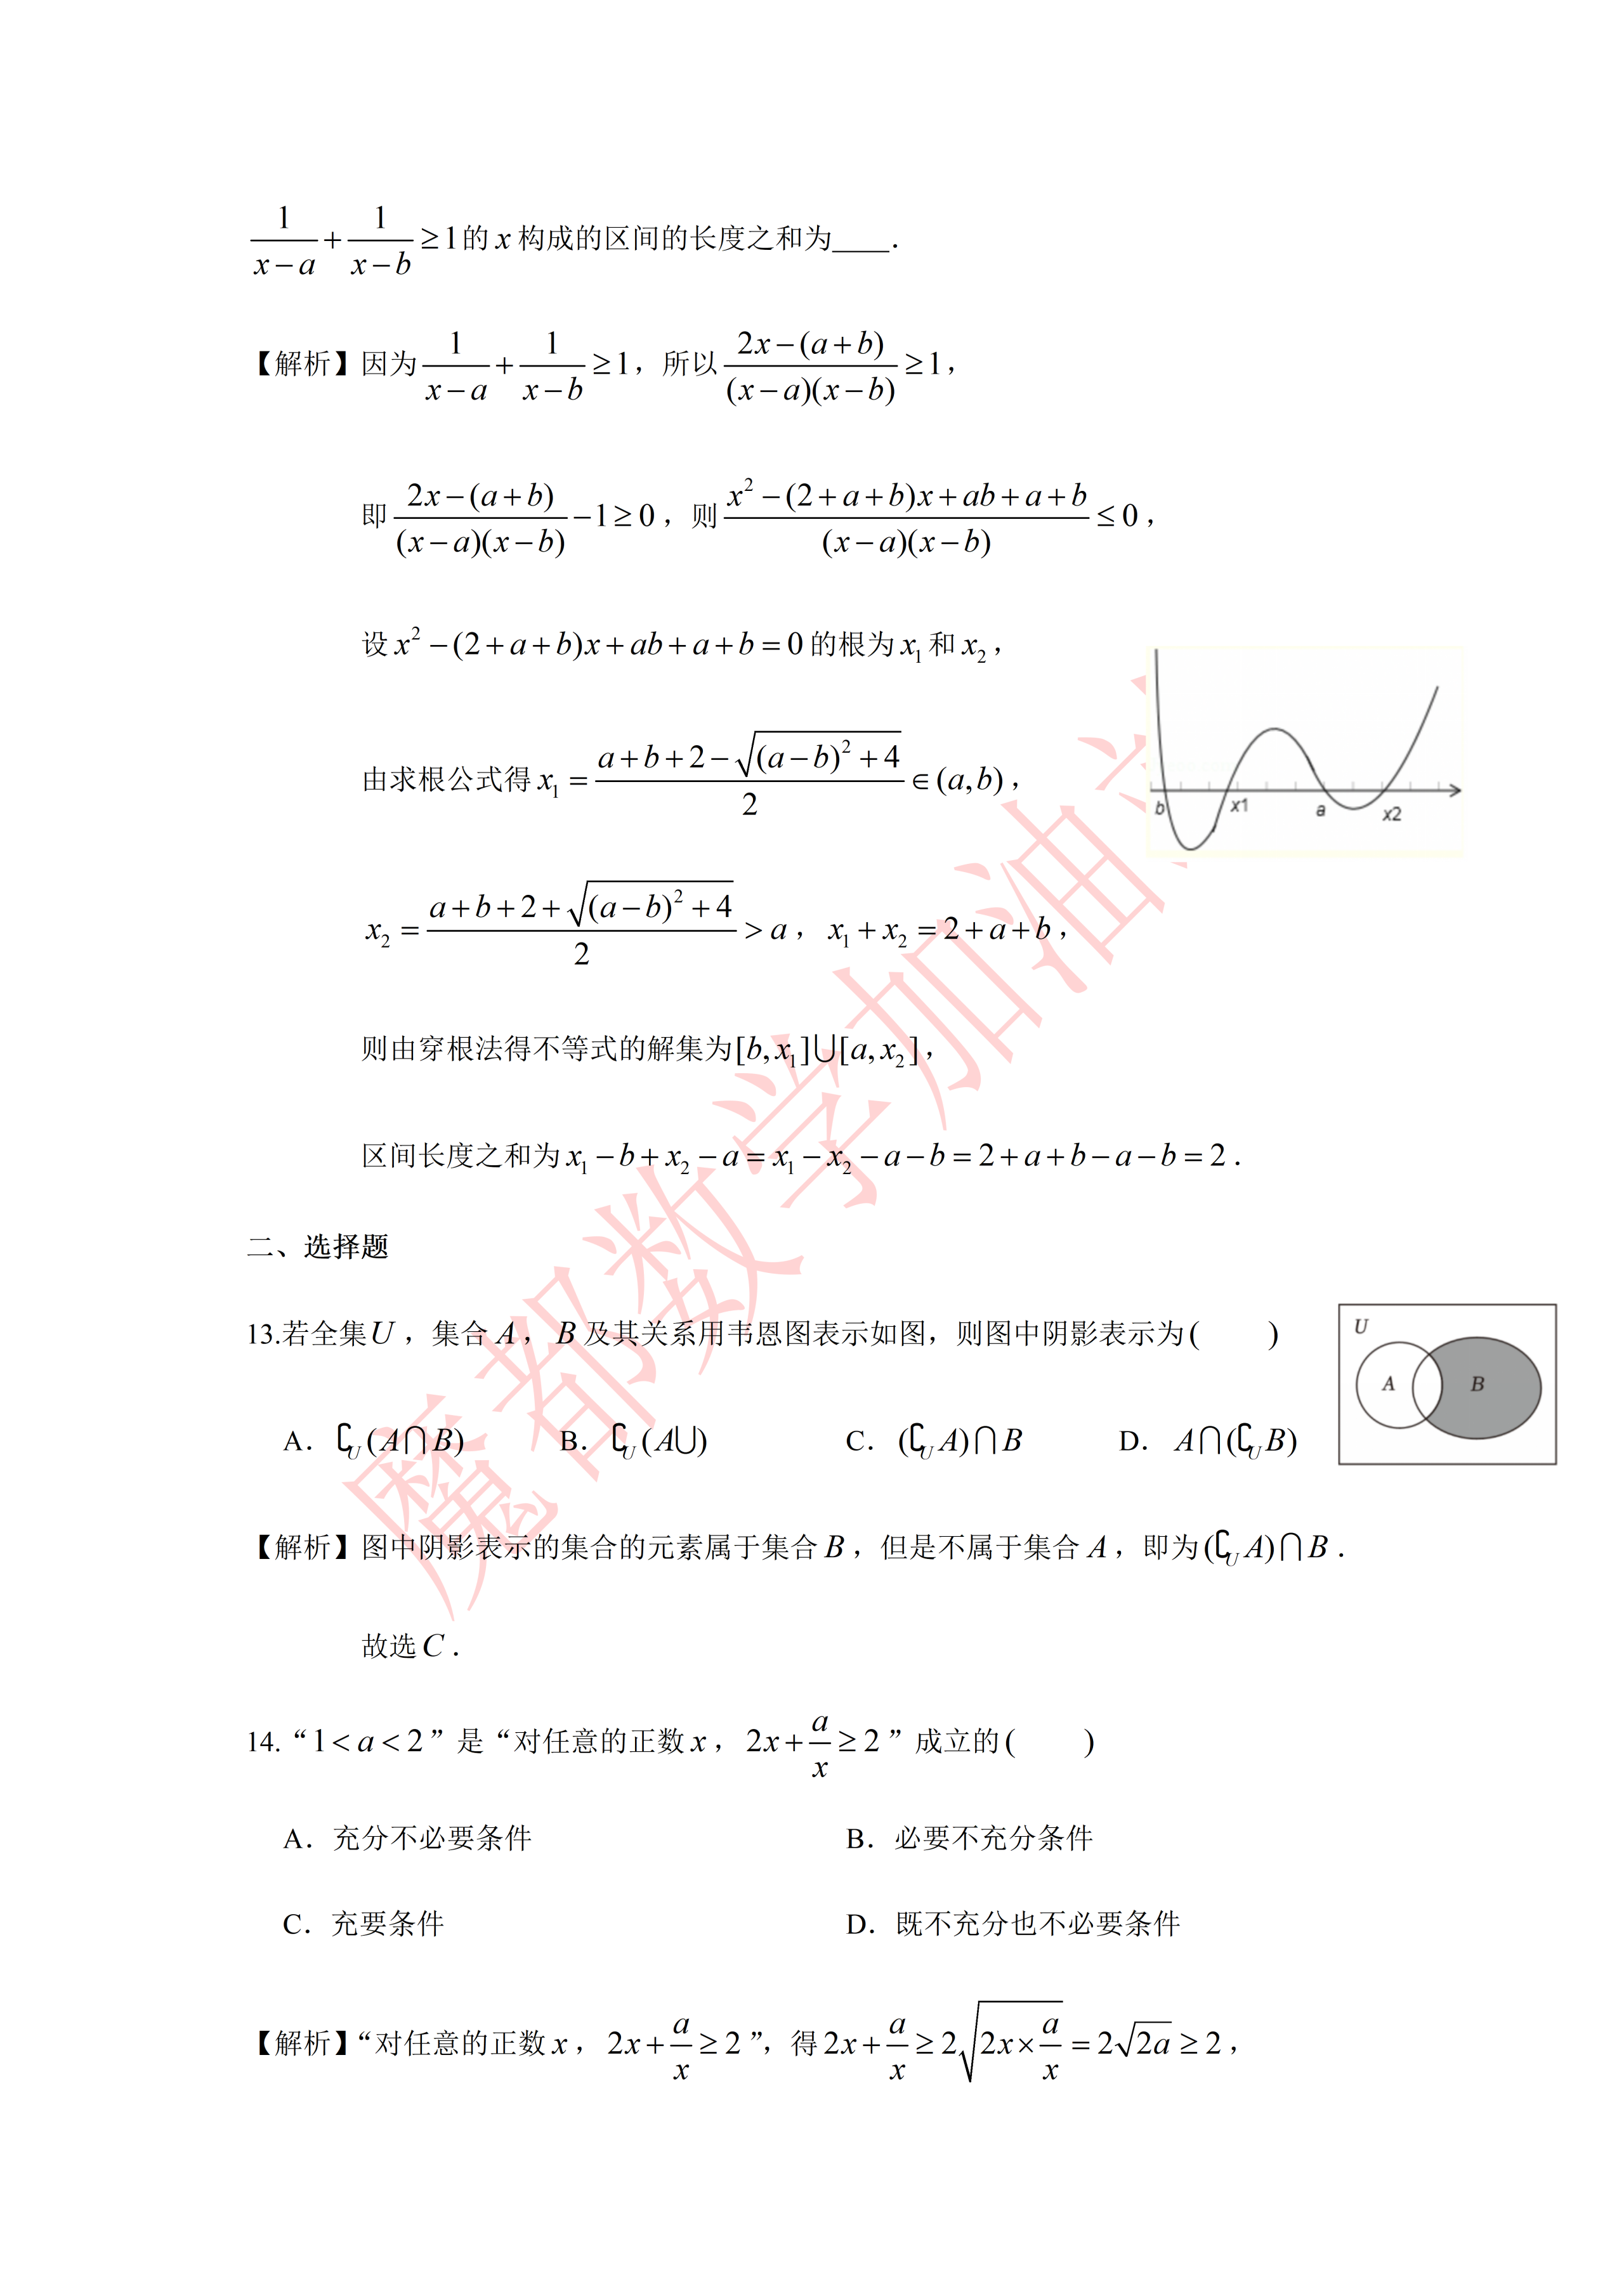
\includegraphics[width=.50\linewidth,trim=1786bp 2255bp 228bp 985bp,clip]{../原图/高一51_华师大二附中_国庆作业3/04.png}
\end{center}
\step{由求根公式得 $x_1=\dfrac{a+b+2-\sqrt{(a-b)^2+4}}{2}\in(a,b)$，}
\step{$x_2=\dfrac{a+b+2+\sqrt{(a-b)^2+4}}{2}>a$，$x_1+x_2=2+a+b$，}
\step{则由穿根法得不等式的解集为 $[b,x_1]\cup[a,x_2]$，}
% 原卷如此，照录未改（此处原卷作 $x_1-x_2$，按上一行 $x_1+x_2=2+a+b$ 当为 $x_1+x_2$）
\step{区间长度之和为 $x_1-b+x_2-a=x_1-x_2-a-b=2+a+b-a-b=2$.}
\solend

\fi

\end{enumerate}

\bigsec{二、选择题}

\begin{enumerate}
\setcounter{enumi}{12}

% 本题是“题干 + 图 + 选项”约 5.5cm 的一整块，图夹在题干与选项之间时 \keepwithprev 挡不住断点，
% 故按 高一30 第 13 题的成例在题前先量一次页高（守卫放在 \item 之前）。
\needvspace{6cm}
\item 若全集 $U$，集合 $A$、$B$ 及其关系用韦恩图表示如图，则图中阴影表示为\mbox{（\quad）}

\begin{center}
% 原卷该图印在题干与选项右侧（原图第 04 页），本稿移作居中排，直接裁取原图，不另存图片文件。
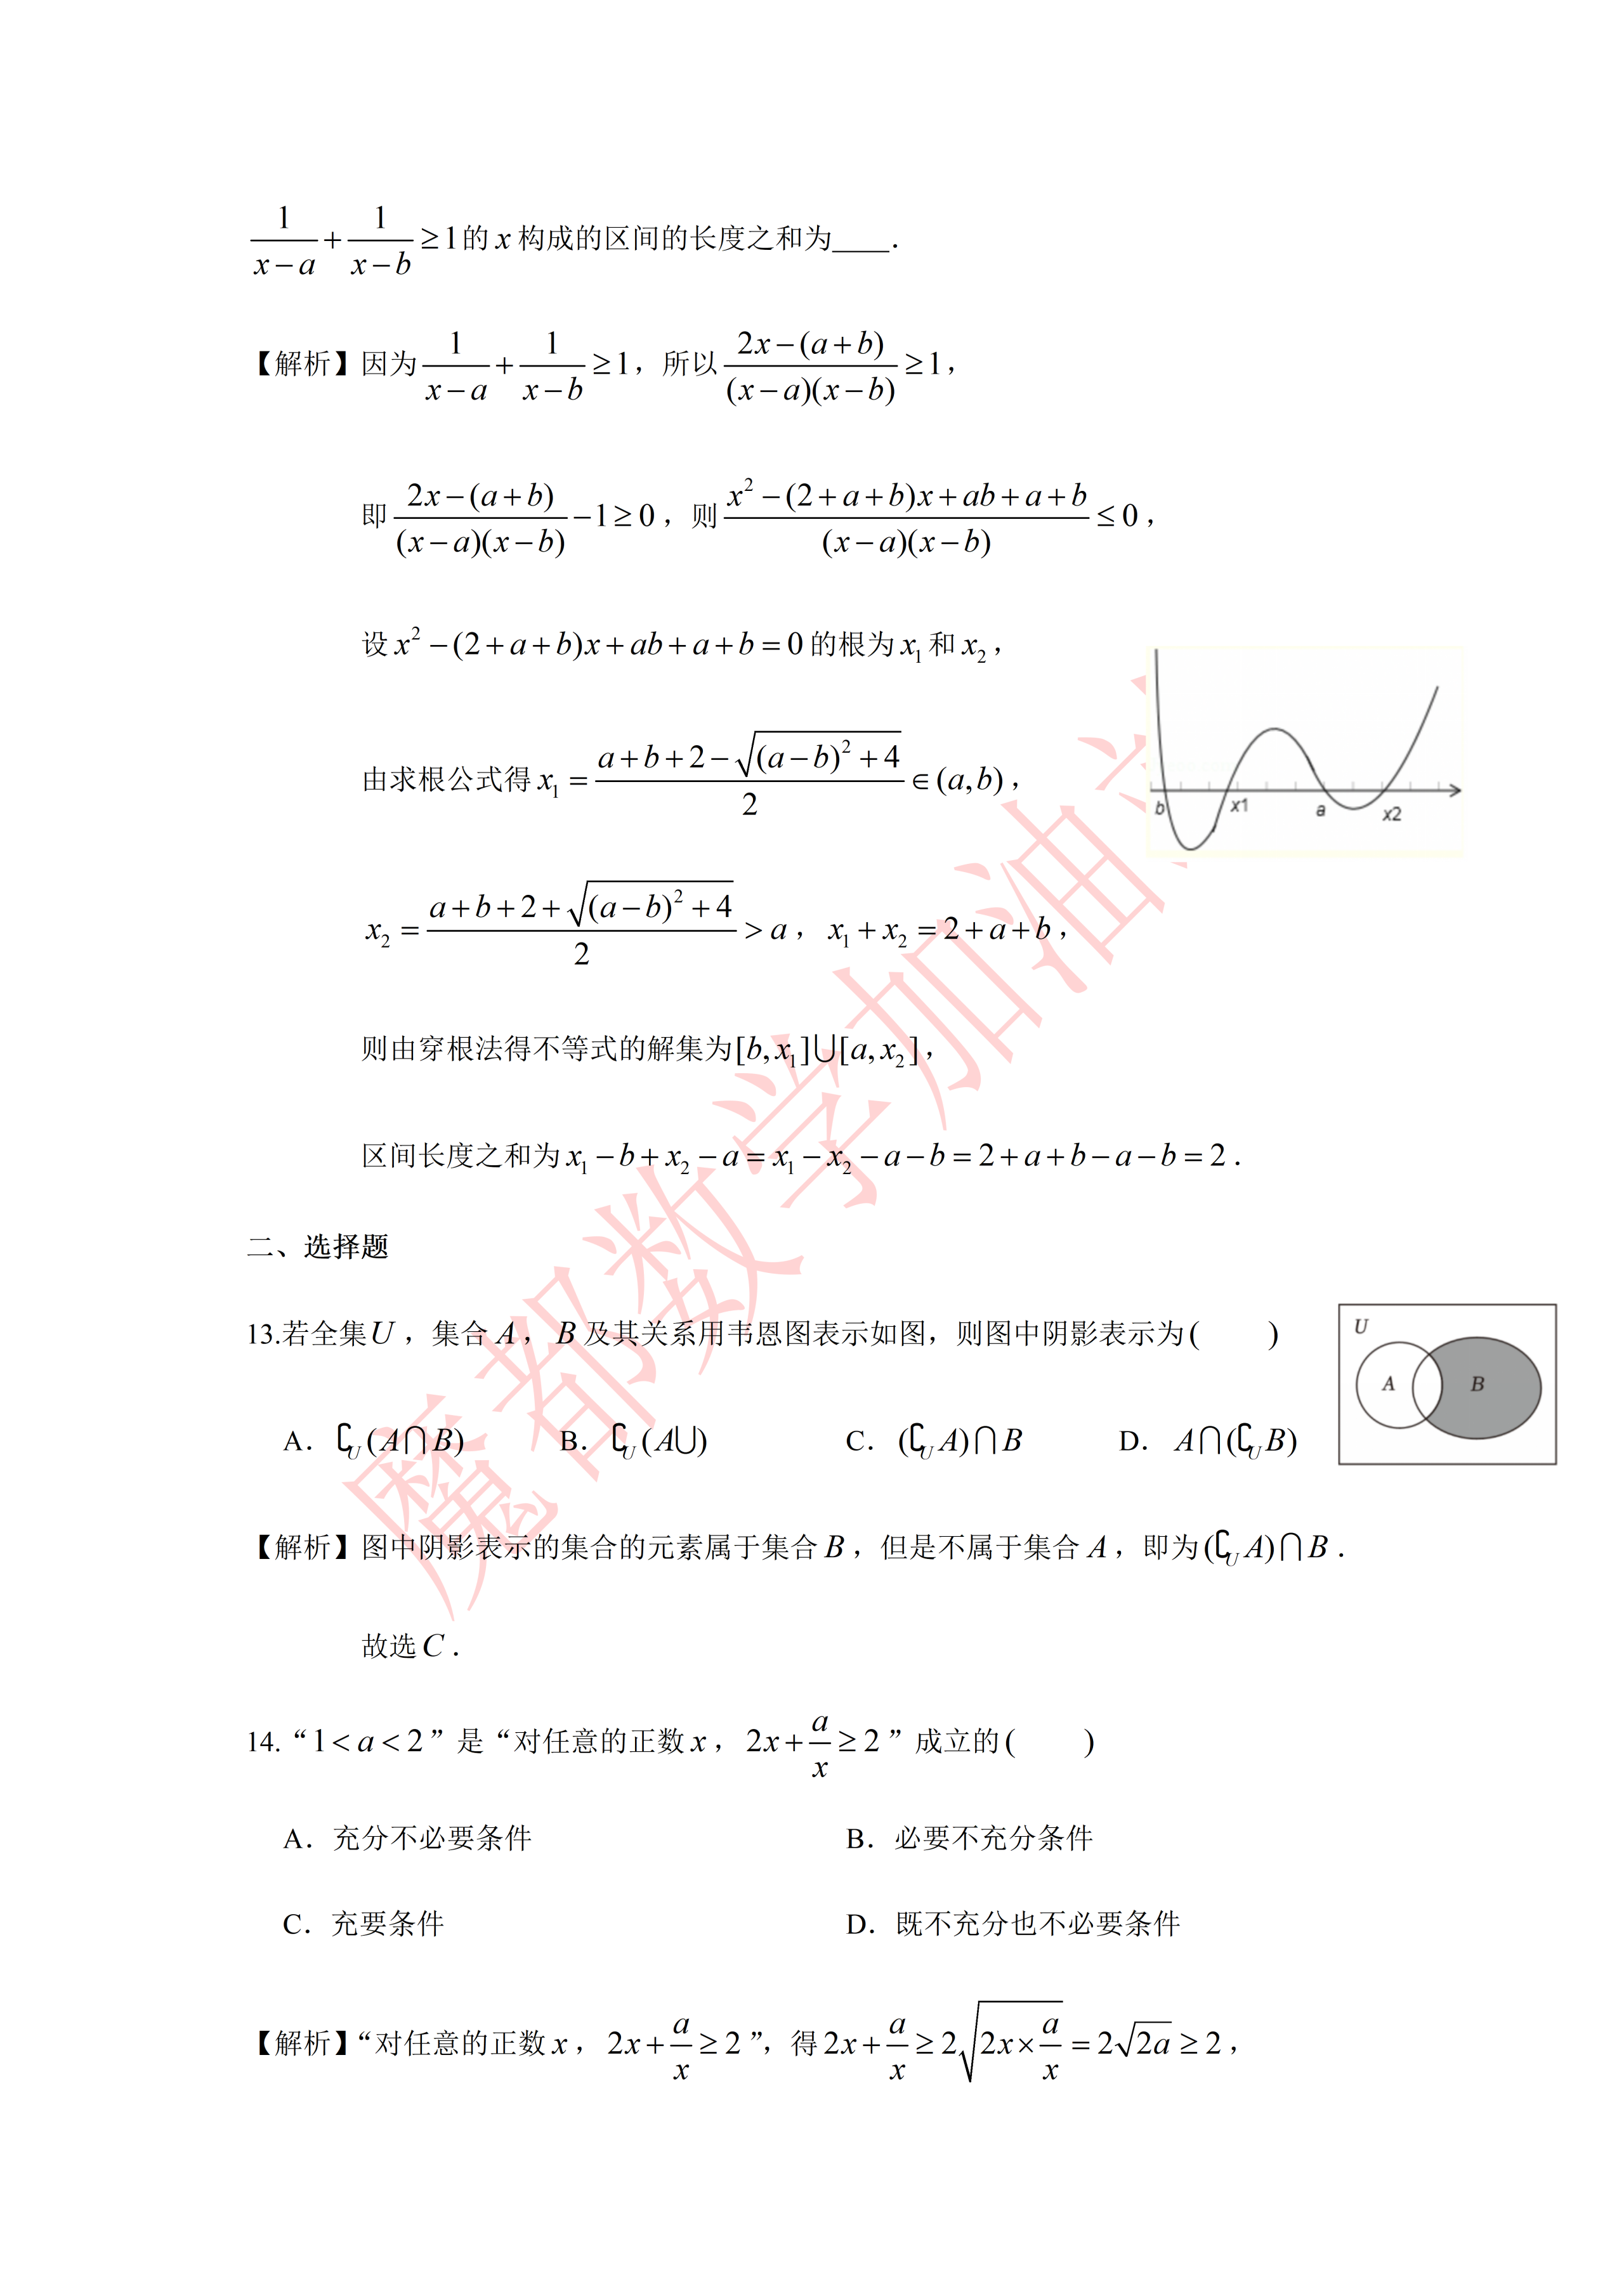
\includegraphics[width=.30\linewidth,trim=2105bp 1308bp 105bp 2050bp,clip]{../原图/高一51_华师大二附中_国庆作业3/04.png}
\end{center}

\keepwithprev
A. $\complement_U(A\cap B)$\qquad B. $\complement_U(A\cup B)$

C. $(\complement_U A)\cap B$\qquad D. $A\cap(\complement_U B)$

\ifanswer
\solbegin
\step{图中阴影表示的集合的元素属于集合 $B$，但是不属于集合 $A$，即为 $(\complement_U A)\cap B$.}
\step{故选 $C$.}
\solend

\fi

\item “$1<a<2$”是“对任意的正数 $x$，$2x+\dfrac ax\geqslant2$”成立的\mbox{（\quad）}

\keepwithprev
A. 充分不必要条件\qquad B. 必要不充分条件

C. 充要条件\qquad\qquad D. 既不充分也不必要条件

\ifanswer
\solbegin
\step{“对任意的正数 $x$，$2x+\dfrac ax\geqslant2$”，得 $2x+\dfrac ax\geqslant2\sqrt{2x\times\dfrac ax}=2\sqrt{2a}\geqslant2$，}
\step{所以 $\sqrt{2a}\geqslant1$，解得 $a\geqslant\dfrac12$，}
\step{若“$1<a<2$”得 $2x+\dfrac ax\geqslant2\sqrt{2x\times\dfrac ax}=2\sqrt{2a}>2\sqrt2>2$，}
\step{所以“$1<a<2$”$\Rightarrow$“对任意的正数 $x$，$2x+\dfrac ax\geqslant2$”，}
\step{所以“$1<a<2$”是“对任意的正数 $x$，$2x+\dfrac ax\geqslant2$”成立的充分不必要条件，}
\step{故选 $A$.}
\solend

\fi

\item 已知函数 $f(x)=2x-3$，$x\in(0,2)$，实数 $a$、$b$ 满足 $f(a)+f(b-1)=0$，则以下成立的有\mbox{（\quad）}

\keepwithprev
A. $a(b-1)$ 的最大值为 $\dfrac94$\qquad\qquad B. $b-\dfrac1a$ 的最大值为 $2$

C. $\dfrac1a+\dfrac1{4b}$ 的最小值为 $\dfrac9{16}$\qquad D. $-1<b-a<3$

\ifanswer
\solbegin
\step{因为函数 $f(x)=2x-3$，$x\in(0,2)$，实数 $a$、$b$ 满足 $f(a)+f(b-1)=0$，}
\step{所以 $2a-3+2(b-1)-3=0$，得 $a+b=4$，$a\in(0,2)$，$b\in(1,3)$，}
\step{所以 $a(b-1)=a(3-a)=-\left(a-\dfrac32\right)^2+\dfrac94$，$a\in(0,2)$，}
\step{所以 $0<a(b-1)\leqslant\dfrac94$，故选项 $A$ 正确；}
\step{$b-\dfrac1a=4-a-\dfrac1a=4-\left(a+\dfrac1a\right)\leqslant4-2=2$，}
\step{当且仅当 $a=1$，$b=3$ 时取等号，又 $b\in(1,3)$，故 $b-\dfrac1a<2$，故 $B$ 错误；}
\step{$\dfrac1a+\dfrac1{4b}=\dfrac14\left(\dfrac1a+\dfrac1{4b}\right)(a+b)=\dfrac14\left(1+\dfrac14+\dfrac ba+\dfrac a{4b}\right)=\dfrac5{16}+\dfrac14\left(\dfrac ba+\dfrac a{4b}\right)$}
\step{$\geqslant\dfrac5{16}+\dfrac14\cdot2\sqrt{\dfrac ba\cdot\dfrac a{4b}}=\dfrac9{16}$，当且仅当 $\dfrac ba=\dfrac a{4b}$，即 $a=2b=\dfrac83$ 时取等号，}
% 原卷如此，照录未改（“又 $a\in(0,2)$，”与下式之间原卷正文夹印“水印”二字）
\step{又 $a\in(0,2)$，水印 $\dfrac1a+\dfrac1{4b}<\dfrac9{16}$，故 $C$ 错误；}
\step{因为 $a\in(0,2)$，$b\in(1,3)$，所以 $-a\in(-2,0)$，所以 $b-a\in(-1,3)$，}
\step{故 $D$ 正确；}
\step{故选 $AD$.}
\solend

\fi

% 本题解析含图（“函数 f(x) 的图像如下”），图夹在解析行间，页末放不下会被拆开，
% 故在题前先量一次页高；上界取“题干 + 选项 + 图 + 首行解析”一块的高度。
\needvspace{6cm}
\item 设 $M_I$ 表示函数 $f(x)=|x^2-4x+2|$ 在闭区间 $I$ 上的最大值. 若正实数 $a$ 满足
$M_{[0,a]}\geqslant2M_{[a,2a]}$，则正实数 $a$ 的取值范围是\mbox{（\quad）}

\keepwithprev
A. $\left[2-\sqrt3,\dfrac12\right]$\qquad B. $[2-\sqrt3,1]$

C. $[2,2+\sqrt3]$\qquad\qquad D. $[2+\sqrt3,4]$

\ifanswer
\solbegin
\step{函数 $f(x)$ 的图像如下：}
\begin{center}
% 原卷该图印在解析行间（原图第 06 页），本稿直接裁取原图，不另存图片文件。
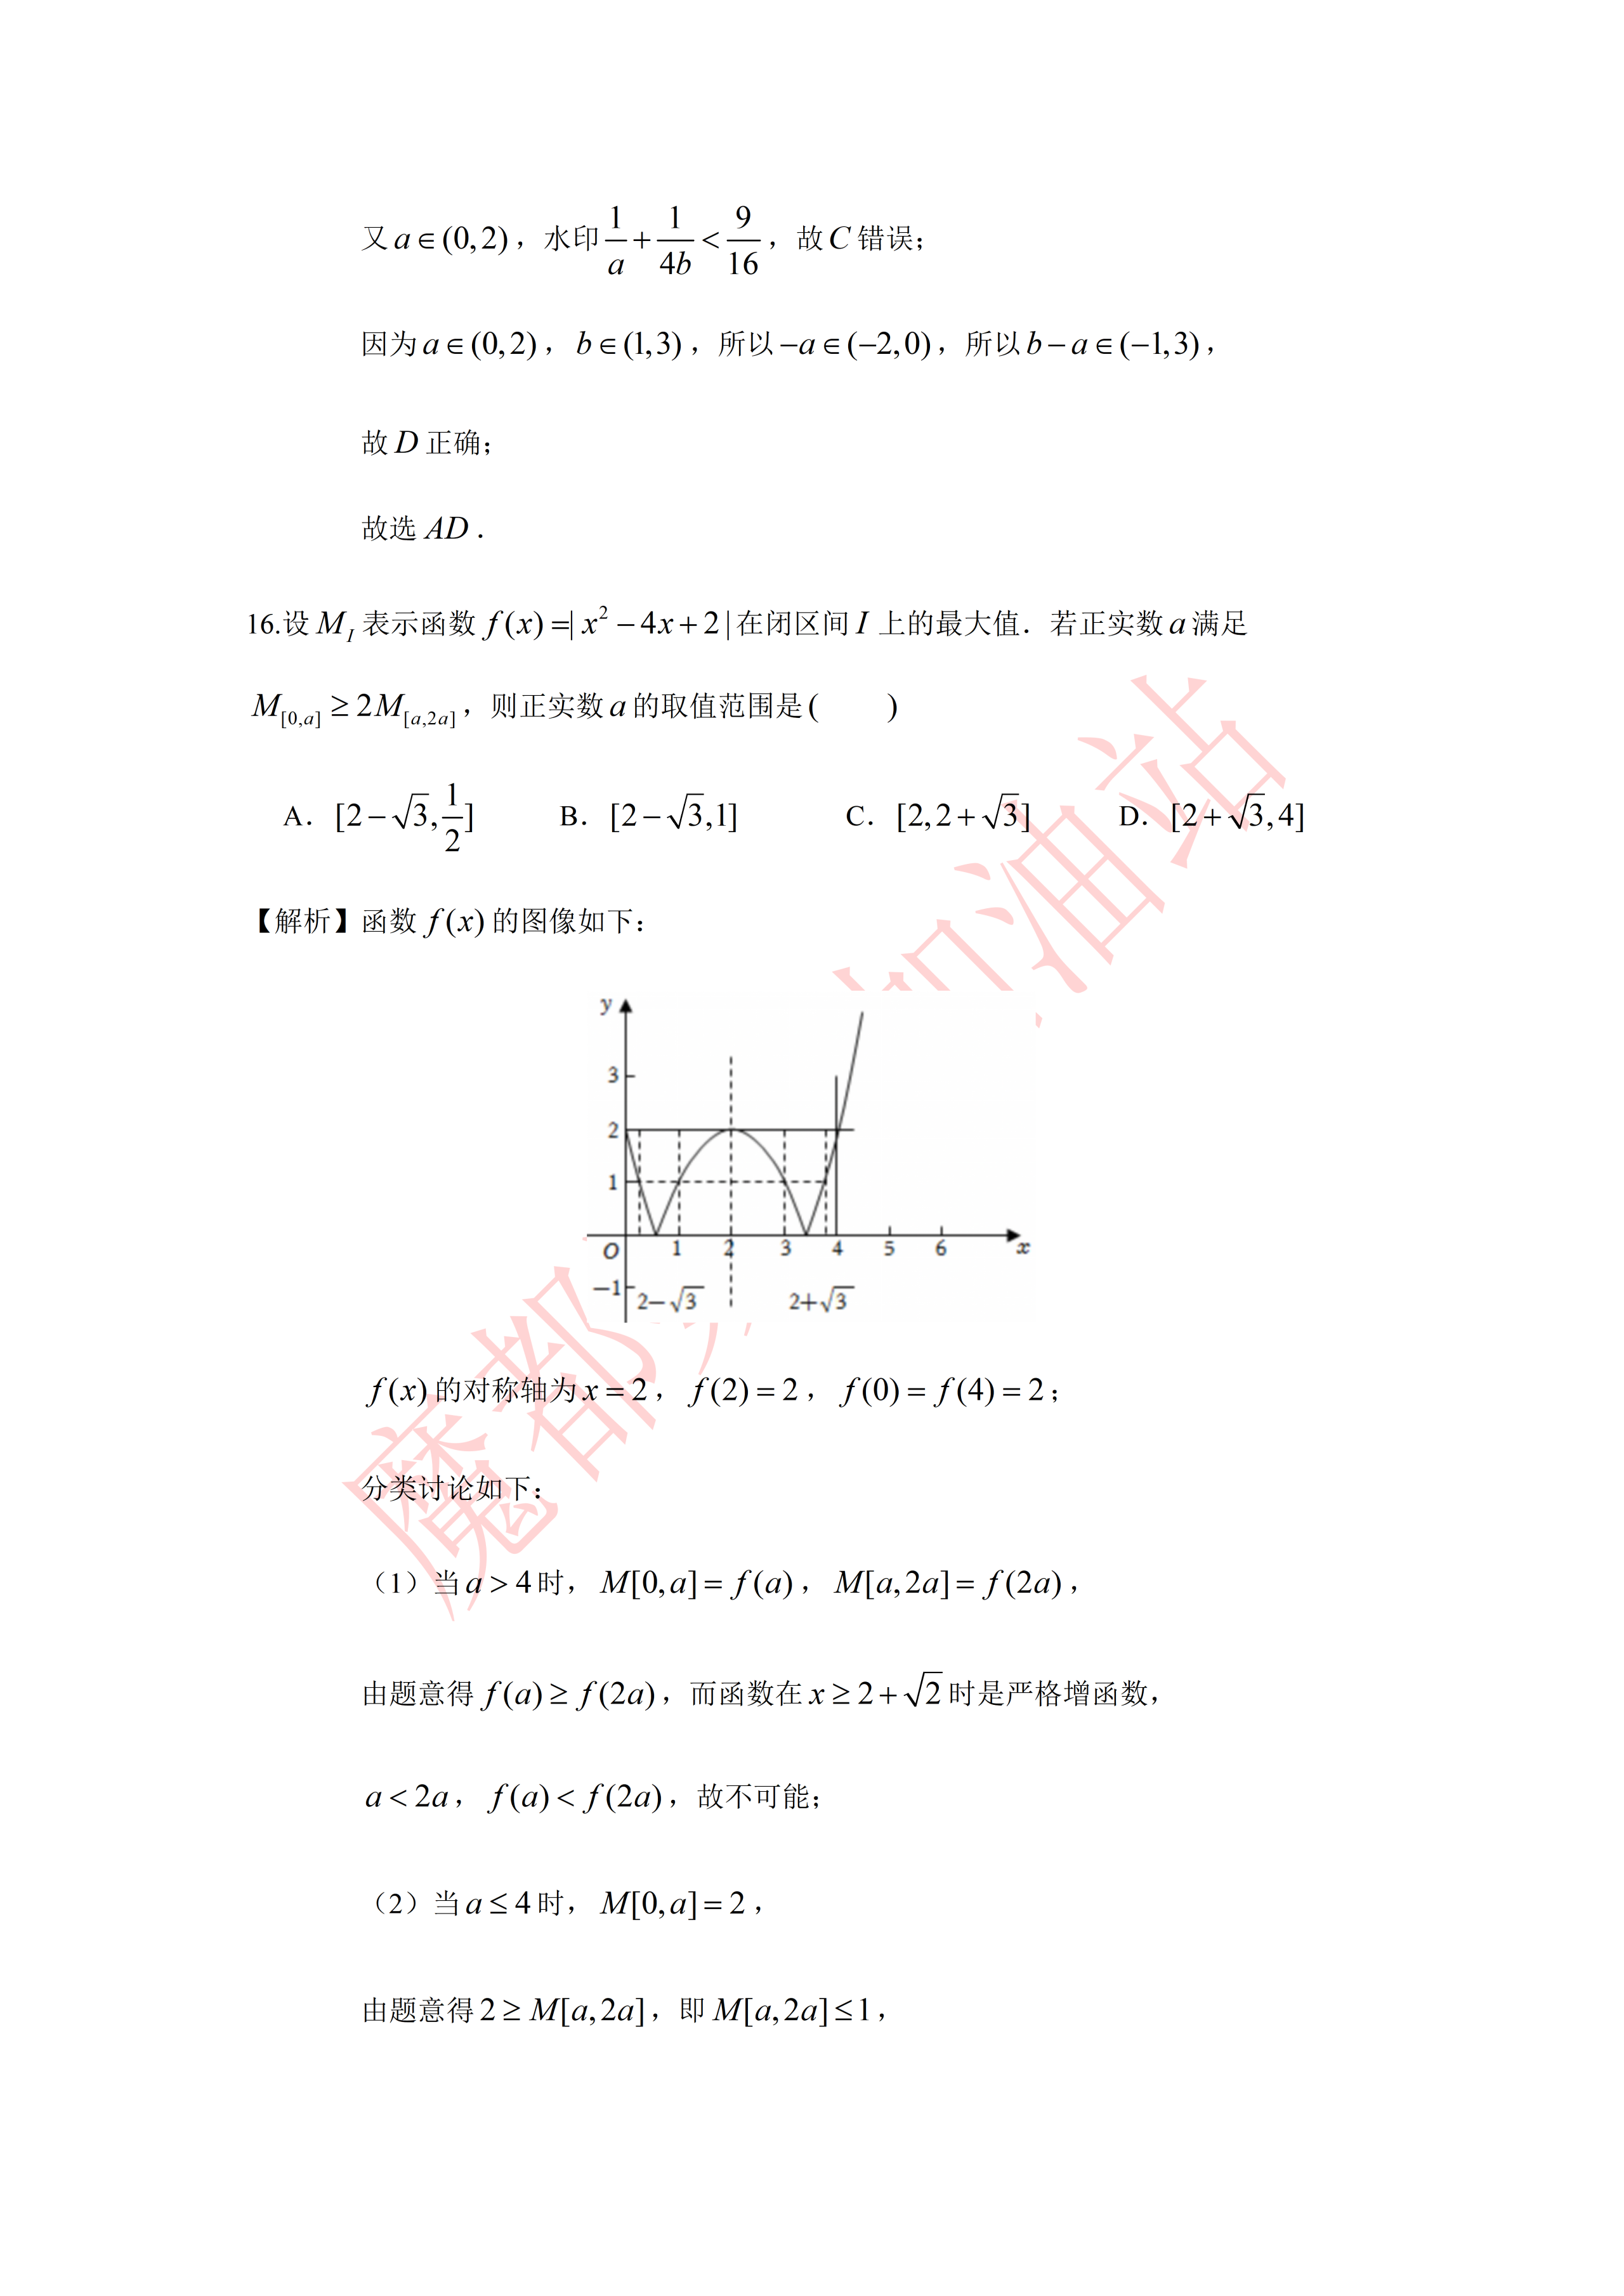
\includegraphics[width=.55\linewidth,trim=895bp 1535bp 915bp 1525bp,clip]{../原图/高一51_华师大二附中_国庆作业3/06.png}
\end{center}
\step{$f(x)$ 的对称轴为 $x=2$，$f(2)=2$，$f(0)=f(4)=2$；}
\step{分类讨论如下：}
\stepm{(1)}{当 $a>4$ 时，$M_{[0,a]}=f(a)$，$M_{[a,2a]}=f(2a)$，}
\step{由题意得 $f(a)\geqslant f(2a)$，而函数在 $x\geqslant2+\sqrt2$ 时是严格增函数，}
\step{$a<2a$，$f(a)<f(2a)$，故不可能；}
\stepm{(2)}{当 $a\leqslant4$ 时，$M_{[0,a]}=2$，}
\step{由题意得 $2\geqslant M_{[a,2a]}$，即 $M_{[a,2a]}\leqslant1$，}
\step{令 $f(x)=1$，解得 $x_1=2-\sqrt3$，$x_2=1$，$x_3=2+\sqrt3$，$x_4=3$，}
\step{则有 $a\geqslant2-\sqrt3$ 并且 $2a\leqslant1$，解得 $2-\sqrt3\leqslant a\leqslant\dfrac12$；}
\step{或者 $a\geqslant3$ 并且 $2a\leqslant2+\sqrt3$，无解；}
\step{故选 $A$.}
\solend

\fi

\end{enumerate}

\bigsec{三、解答题}

\begin{enumerate}
\setcounter{enumi}{16}

\item 已知 $M=\{x\mid2\leqslant x\leqslant5\}$，$N=\{x\mid a-1\leqslant x\leqslant2a+1\}$.
\begin{enumerate}[label=(\arabic*)]
\item 若 $M\subseteq N$，求实数 $a$ 的取值范围；
\item 若 $M\supseteq N$，求实数 $a$ 的取值范围.
\end{enumerate}

\ifanswer
\ans{（1）$[2,3]$；（2）$(-\infty,-2)$}
\fi

\ansspace[6]

\item 设集合 $A=\{x\mid|x+1|\leqslant3\}$，$B=\{x\mid0<x<3m\}$.
\begin{enumerate}[label=(\arabic*)]
\item 若 $A\cup B=A$，求实数 $m$ 的取值范围；
\item 设 $P=(\complement_R A)\cap B$，若 $\exists x\in\Z$ 且 $x\in P$，求实数 $m$ 的取值范围.
\end{enumerate}

\ifanswer
\solbegin
\stepm{(1)}{$A=\{x\mid|x+1|\leqslant3\}=\{x\mid-4\leqslant x\leqslant2\}$，且 $A\cup B=A$，所以 $B\subseteq A$.}
\step{若 $B=\varnothing$，此时 $0\geqslant3m$，解得 $m\leqslant0$；}
\step{若 $B\neq\varnothing$，此时 $0<3m$，且 $3m\leqslant2$，解得 $0<m\leqslant\dfrac23$；}
\step{则实数 $m$ 的取值范围是 $\left(-\infty,\dfrac23\right]$.}
\stepm{(2)}{因为 $\exists x\in\Z$ 且 $x\in P$，所以集合 $P$ 中至少存在一个整数.}
\step{$\complement_R A=\{x\mid x<-4\text{ 或 }x>2\}$，$B=\{x\mid0<x<3m\}$，}
\step{要使 $P=(\complement_R A)\cap B$ 中至少存在一个整数，则 $\begin{cases}3m>0\\3m>3\end{cases}$，解得 $m>1$，}
\step{则实数 $m$ 的取值范围是 $(1,+\infty)$.}
\solend

\fi

\ansspace[7]

\item 已知函数 $f(x)=x^2+(1-a)x-a(a\in\R)$.
\begin{enumerate}[label=(\arabic*)]
\item 解关于 $x$ 的不等式 $f(x)<0$；
\item 若 $\forall a\in[-1,1]$，$f(x)\geqslant0$ 恒成立，求实数 $x$ 的取值范围.
\end{enumerate}

\ifanswer
\solbegin
\stepm{(1)}{不等式 $x^2+(1-a)x-a<0$ 等价于 $(x-a)(x+1)<0$，}
\step{当 $a<-1$ 时，不等式的解集为 $(a,-1)$；}
\step{当 $a=-1$ 时，不等式的解集为 $\varnothing$；}
\step{当 $a>-1$ 时，不等式的解集为 $(-1,a)$.}
\stepm{(2)}{$x^2+(1-a)x-a=-a(x+1)+x^2+x$，}
\step{设 $g(a)=-a(x+1)+x^2+x$，$a\in[-1,1]$，}
\step{要使 $g(a)\geqslant0$ 在 $a\in[-1,1]$ 上恒成立，}
\step{只需 $\begin{cases}g(-1)\geqslant0\\g(1)\geqslant0\end{cases}$，即 $\begin{cases}x^2+2x+1\geqslant0\\x^2-1\geqslant0\end{cases}$，解得 $x\geqslant1$ 或 $x\leqslant-1$，}
\step{所以 $x$ 的取值范围为 $\{x\mid x\leqslant-1\text{ 或 }x\geqslant1\}$.}
\solend

\fi

\ansspace[7]

\item 若实数 $x$、$y$、$m$ 满足 $|x-m|>|y-m|$，则称 $x$ 比 $y$ 远离 $m$.
\begin{enumerate}[label=(\arabic*)]
\item 若 $2$ 比 $3x-4$ 远离 $1$，求 $x$ 的取值范围；
\item 设 $y=\dfrac{x+2}{x+1}$，其中 $x\in(0,\sqrt2)\cup(\sqrt2,+\infty)$，判断：$x$ 与 $y$ 哪一个更远离 $\sqrt2$？并说明理由.
\item 若 $x+y=2$，试问：$y$ 与 $x^2+y^2$ 哪一个更远离 $\dfrac12$？并说明理由.
\end{enumerate}

\ifanswer
\solbegin
\stepm{(1)}{由题意得 $|2-1|>|3x-4-1|$，所以 $|3x-5|<1$，解得 $\dfrac43<x<2$，}
\step{故 $x$ 的取值范围为 $\left(\dfrac43,2\right)$；}
\stepm{(2)}{$x$ 比 $y$ 更远离 $\sqrt2$，}
\step{理由如下：要证 $x$ 比 $y$ 更远离 $\sqrt2$，只要证 $|x-\sqrt2|>\left|\dfrac{x+2}{x+1}-\sqrt2\right|$，}
\step{即证 $|x-\sqrt2|>\left|\dfrac{(1-\sqrt2)(x-\sqrt2)}{x+1}\right|$，}
\step{因为 $x\in(0,\sqrt2)\cup(\sqrt2,+\infty)$，所以 $|x-\sqrt2|>0$，}
\step{所以只要证 $1>\dfrac{\sqrt2-1}{|x+1|}$，即证 $|x+1|>\sqrt2-1$，}
\step{因为 $x\in(0,\sqrt2)\cup(\sqrt2,+\infty)$，所以 $x+1\in(1,\sqrt2+1)\cup(\sqrt2+1,+\infty)$，}
\step{所以 $|x+1|>1>\sqrt2-1$，所以 $x$ 比 $y$ 更远离 $\sqrt2$；}
\stepm{(3)}{因为 $x^2+y^2\geqslant\dfrac{(x+y)^2}{2}=2$，当且仅当 $x=y=1$ 时等号成立，}
\step{所以 $\left|x^2+y^2-\dfrac12\right|=x^2+y^2-\dfrac12$，}
\step{从而 $\left|y-\dfrac12\right|-\left|x^2+y^2-\dfrac12\right|=\left|y-\dfrac12\right|-\left(x^2+y^2-\dfrac12\right)$，}
\step{①$y\geqslant\dfrac12$，$\left|y-\dfrac12\right|-\left|x^2+y^2-\dfrac12\right|=y-\dfrac12-\left(x^2+y^2-\dfrac12\right)=y-x^2-y^2$}
\step{$=y-(2-y)^2-y^2=-2y^2+5y-4=-2\left(y-\dfrac54\right)^2-\dfrac78<0$，}
\step{即 $\left|y-\dfrac12\right|<\left|x^2+y^2-\dfrac12\right|$；}
\step{②$y<\dfrac12$，}
\step{$\left|y-\dfrac12\right|-\left|x^2+y^2-\dfrac12\right|=\left(\dfrac12-y\right)-\left(x^2+y^2-\dfrac12\right)=-y-x^2-y^2+1$}
\step{$=-y-(2-y)^2-y^2+1=-2y^2+3y-3=-2\left(y-\dfrac34\right)^2-\dfrac{15}8<0$，}
\step{即 $\left|y-\dfrac12\right|<\left|x^2+y^2-\dfrac12\right|$；}
\step{综上，$\left|y-\dfrac12\right|<\left|x^2+y^2-\dfrac12\right|$，即 $x^2+y^2$ 比 $y$ 更远离 $\dfrac12$.}
\solend

\fi

\ansspace[9]

\item 对于非空有限整数集 $X$，$m\in\N^*$，定义 $X^m=\{x^m\mid x\in X\}$，对 $n\in\Z$，
$Y\oplus n=\{x+n\mid x\in Y\}$ 现有两个非空有限整数集 $A$、$B$，已知 $A\oplus1\subseteq B$ 且
$B^2\oplus(-4)\subseteq A$.
\begin{enumerate}[label=(\arabic*)]
\item 当 $A=\{-3,0\}$ 时求集合 $B$；
\item 证明：$A\subseteq\{-3,-2,0,1\}$；
\item 当 $A\oplus1=B$ 且 $B^2\oplus(-4)=A$ 时，任取 $a\in A$，$b\in B$ 构造函数
$f(x)=(x-a)(x-b)$ 问：当 $a$、$b$ 取何值时，$f(x)$ 的最小值最小？
\end{enumerate}

\ifanswer
\solbegin
\stepm{(1)}{因为 $A=\{-3,0\}$，$B^2\oplus(-4)\subseteq A$，}
\step{所以 $B^2\oplus(-4)$ 可能为 $\varnothing$、$\{-3\}$、$\{0\}$、$\{-3,0\}$，}
\step{当 $B^2\oplus(-4)=\varnothing$ 时 $B^2=\varnothing$，不满足非空，不合题意；}
\step{当 $B^2\oplus(-4)=\{-3\}$ 时 $B^2=\{1\}$，所以 $B=\{1,-1\}$、$\{1\}$、$\{-1\}$，}
\step{当 $B^2\oplus(-4)=\{0\}$ 时 $B^2=\{4\}$，所以 $B=\{2,-2\}$、$\{2\}$、$\{-2\}$，}
% 原卷如此，照录未改（此处作 $\{0,-3\}$，上一行同一集合作 $\{-3,0\}$）
\step{当 $B^2\oplus(-4)=\{0,-3\}$ 时 $B^2=\{4,1\}$，}
\step{所以 $B=\{1,2,-1,-2\}$、$\{2,-1,-2\}$、$\{2,1,-2\}$、$\{1,-1,-2\}$、$\{1,-1,2\}$、$\{1,2\}$、$\{-1,2\}$、$\{-1,-2\}$、$\{1,-2\}$，}
\step{又 $A\oplus1=\{-2,1\}\subseteq B$，得 $B$ 为 $\{1,-2\}$、$\{2,1,-2\}$、$\{1,-1,-2\}$、$\{1,2,-1,-2\}$.}
\stepm{(2)}{设 $x\in A$，因为 $A\oplus1\subseteq B$，所以 $x+1\in B$，}
\step{又 $B^2\oplus(-4)\subseteq A$，所以 $(x+1)^2-4\in A$，}
% 原卷如此，照录未改（此处及下文取 $x=2$ 处原卷均作 $(-4+1)^2-4=52-2a>0$）
\step{取 $x=-4$，则 $(-4+1)^2-4=52-2a>0$，$(5+1)^2-4=32\in A$，$\cdots$，}
\step{无限迭代，而 $A$ 为有限集，不合题意，舍去，即 $-4\notin A$；}
\step{取 $x=-3$，则 $(-3+1)^2-4=0\in A$，$(0+1)^2-4=-3\in A$，}
\step{得 $A$ 集合可为 $\{-3,0\}$；}
\step{取 $x=-2$，则 $(-2+1)^2-4=-3\in A$，$(-3+1)^2-4=0\in A$，}
\step{$(0+1)^2-4=-3\in A$，得 $A$ 集合可为 $\{-3,-2,0\}$；}
\step{取 $x=-1$，则 $(-1+1)^2-4=-4\in A$，又 $-4\notin A$，所以 $-1\notin A$，}
\step{取 $x=1$，则 $(1+1)^2-4=0\in A$，$(0+1)^2-4=-3\in A$，}
\step{$(-3+1)^2-4=0\in A$，得 $A$ 集合可为 $\{-3,0,1\}$，}
\step{取 $x=2$，则 $(2+1)^2-4=52-2a>0$，$(5+1)^2-4=32\in A$，$\cdots$，}
\step{无限迭代，而 $A$ 为有限集，不合题意，舍去，即 $2\notin A$，}
\step{同理当 $x<-4$ 或 $x>2$，且 $x\in\Z$ 时不符合 $A$ 为有限集，舍去；}
\step{故由上得 $A$ 集合可为 $\{-3,0\},\{-3,-2,0\},\{-3,0,1\},\{-3,-2,0,1\}$，}
\step{所以 $A\subseteq\{-3,-2,0,1\}$，}
\stepm{(3)}{当 $A\oplus1=B$ 且 $B^2\oplus(-4)=A$ 时，}
\step{设 $x\in B$，则 $x^2-4\in B^2\oplus(-4)=A$，}
% 原卷如此，照录未改（题设 $A=\{-3,0\}$，此处两个判别式取的是 $-2$ 与 $1$，均不属于 $A$）
\step{$x^2-4=-2$ 时 $x=\pm\sqrt2$，不为整数，不合题意；}
\step{$x^2-4=1$ 时 $x=\pm\sqrt5$，不为整数，不合题意；}
\step{所以 $A=\{-3,0\}$，又 $A\oplus1=B$，则 $B=\{-2,1\}$，}
\step{任取 $a\in A$，$b\in B$ 构造函数 $f(x)=(x-a)(x-b)$，}
\step{$f(x)=(x-a)(x-b)=x^2-(a+b)x+ab$}
\step{$=x^2-(a+b)x+\dfrac{(a+b)^2}{4}+ab-\dfrac{(a+b)^2}{4}$}
\step{$=\left[x-\dfrac{(a+b)}2\right]^2-\dfrac{(a-b)^2}{4}\geqslant-\dfrac{(a-b)^2}{4}$，所以 $f(x)_{min}=-\dfrac{(a-b)^2}{4}$，}
\step{又 $a\in A=\{-3,0\}$，$b\in B=\{-2,1\}$，所以 $a-b$ 的取值有 $-1,-4,2$，}
\step{所以 $f(x)_{min}=-\dfrac{(a-b)^2}{4}\geqslant-\dfrac{(-3-1)^2}{4}=-4$，}
\step{即当 $a=-3$，$b=1$ 时 $f(x)_{min}$ 的最小值为 $-4$.}
\solend

\fi

\ansspace*[12]

\end{enumerate}

\end{document}
"
% 紧凑版：xelatex "\def\iscompact{1}% 高一51_华师大二附中_国庆作业3.tex
%   —— 高一上数学“2026-2027 年华师大二附中高一上国庆作业 3”（讲评版）
% 试卷版：xelatex 高一51_华师大二附中_国庆作业3.tex
% 答案版：xelatex "\def\isanswer{1}% 高一51_华师大二附中_国庆作业3.tex
%   —— 高一上数学“2026-2027 年华师大二附中高一上国庆作业 3”（讲评版）
% 试卷版：xelatex 高一51_华师大二附中_国庆作业3.tex
% 答案版：xelatex "\def\isanswer{1}\input{高一51_华师大二附中_国庆作业3.tex}"
% 紧凑版：xelatex "\def\iscompact{1}\input{高一51_华师大二附中_国庆作业3.tex}"
%
% 原始材料：微信公众号“魔都数学加油站”文章，作者破晓，连载“27学年高一51”；
% 原文标题“27学年高一51——2026-2027年上海市华师大二附中高一上国庆作业3”；
% 原文链接：https://mp.weixin.qq.com/s/95SLMEmPUT30s4U7wjr5Og。
% 该页面用 JS 渲染，未见明确发布日期；页面内时间戳约为 2026-10-05 21:37，本稿以该时刻记可得日期。
% 正文为 12 张 PNG 页：第 01、02、03、05、07、08、11 页 4762×6735，
% 第 04、06、09、10、12 页 2560×3620。按页序逐页读取，12 页全为试卷正文页
% （卷首标题在第 1 页页顶，卷末解答题止于第 12 页），无封面页、目录页或单独的页脚页。
% 卷面标题照原卷印作“2026-2027 年华师大二附中高一上国庆作业 3”（公众号标题中的“上海市”
% 卷面标题行没有，本稿照卷面），年份区间按全稿惯例排 en dash。
%
% 篇幅与题号：原卷自第 3 题起编号（第 1、2 题不在本卷内）。填空题 3—12（10 题）、
% 选择题 13—16（4 题）、解答题 17—21（5 题），共 19 题。本稿沿用原节与原题号，
% 只改排为全稿统一的大节样式（原卷小节标题为“一、填空题”“二、选择题”“三、解答题”）。
% 正文为讲评版：填空题 3—12 与选择题 13—16 只印【解析】（选择题的结论“故选 X”印在解析内），
% 按全稿口径这类题不另提 \ans{}；解答题第 17 题只印【答案】，故只给 \ans{}；
% 第 18—21 题只印【解析】。
%
% 副标题：原卷未印副标题。本稿按“知识模块”口径标作“集合与常用逻辑用语、不等式”：
% 19 题中集合与常用逻辑用语 8 题（3、4、6、10、13、17、18、21），
% 不等式（含函数最值、绝对值不等式）11 题（5、7、8、9、11、12、14、15、16、19、20），
% 两类均远超三分之一，故并标。口径同 高一46_交附闵行_国庆作业3、高一48_华师大二附中_周末作业2。
%
% 与原卷的排版差异：
%   ① 原卷每题下直接印【答案】或【解析】，本稿按全稿惯例将答案与解析置于答案版；
%   ② 原卷未印副标题，本稿按“知识模块”口径补出；
%   ③ 原卷填空横线按全稿惯例排为 \blankline[4.4em]；
%   ④ 原卷 $R$、$N$、$Z$ 均排斜体，本稿按全稿惯例改用花体 $\R$、$\N$、$\Z$（同 高一48）；
%   ⑤ 原卷第 12 题解析配图、第 13 题题干韦恩图都印在正文右侧的浮动位置，第 16 题解析配图
%      印在解析行间；本稿三图一律居中排，均自原图对应页裁切（trim），不另存图片文件；
%   ⑥ 原卷解答题未留作答空白，本稿按全稿惯例加 \ansspace；
%   ⑦ 原卷第 15 题解析第 7、8 两个印刷行是一串连等式的折行，本稿按“一条 \step ＝ 一个印刷行”
%      的口径分成两条 \step。
%
% 原卷笔误/存疑（均照录未改，正文对应处另有 % 注）：
%   ① 第 12 题解析末行作“区间长度之和为 $x_1-b+x_2-a=x_1-x_2-a-b=2+a+b-a-b=2$”，
%      按上一行 $x_1+x_2=2+a+b$，此处应为 $x_1+x_2$；原卷作 $x_1-x_2$。
%   ② 第 15 题解析“又 $a\in(0,2)$，”与 $\dfrac1a+\dfrac1{4b}<\dfrac9{16}$ 之间，
%      原卷正文夹印“水印”二字（系制版遗留字样，非试卷内容）。
%   ③ 第 21 题第 (2) 问解析两处（取 $x=-4$、取 $x=2$）作“$=52-2a>0$”，
%      与题设 $(x+1)^2-4$ 的取值（按 $x=-4$ 应为 $5$）不符，当系原卷算式遗留。
%   ④ 第 21 题第 (1) 问解析先写 $B^2\oplus(-4)$ 可能为 $\{-3,0\}$，后文又作 $\{0,-3\}$，
%      同一集合两种写法。
%   ⑤ 第 21 题第 (3) 问解析：题设 $B^2\oplus(-4)=A$ 且 $A=\{-3,0\}$ 时，由 $x^2-4\in A$
%      应得 $x^2-4=-3$ 或 $0$；原卷讨论的却是 $x^2-4=-2$ 与 $x^2-4=1$（两值均不属于 $A$），
%      与题设不合。
%
% 插图：3 张，均自原图裁切（无 \begin{tikzpicture} 重排）：
%   · 第 13 题题干韦恩图（原图第 04 页，图在题干与选项右侧）
%   · 第 12 题解析配图（原图第 04 页，图在解析右侧）
%   · 第 16 题解析配图（原图第 06 页，图在解析中间）
%
\documentclass[a4paper,11pt]{article}
\usepackage{common}

\begin{document}

\examtitlest[3]{2026--2027 年华师大二附中高一上国庆作业 3}{集合与常用逻辑用语、不等式}

\bigsec{一、填空题}

\begin{enumerate}
\setcounter{enumi}{2}

\item 若 $\{x\mid x<1\text{ 或 }x>4\}\cup\{x\mid m<x<2m+3\}=R$，则实数 $m$ 的取值范围为\blankline[4.4em].

\ifanswer
\solbegin
\step{因为 $\{x\mid x<1\text{ 或 }x>4\}\cup\{x\mid m<x<2m+3\}=R$，}
\step{所以 $\begin{cases}m<1\\2m+3>4\end{cases}$，解得 $\dfrac12<m<1$，所以 $m$ 的取值范围为 $\left(\dfrac12,1\right)$.}
\solend

\fi

\item 若“$x\leqslant5$”是“$x<a$”的必要不充分条件，则 $a$ 的取值范围是\blankline[4.4em].

\ifanswer
\solbegin
\step{若“$x\leqslant5$”是“$x<a$”的必要不充分条件，则 $\{x\mid x<a\}\subset\{x\mid x\leqslant5\}$，}
\step{所以 $a\leqslant5$.}
\solend

\fi

\item 实数 $x$、$y$ 满足 $x^2+2xy+4y^2=1$，则 $x+2y$ 的取值范围是\blankline[4.4em].

\ifanswer
\solbegin
\step{因为 $x^2+2xy+4y^2=(x+2y)^2-2xy=1$，}
\step{所以 $(x+2y)^2-1=x\cdot(2y)\leqslant\left(\dfrac{x+2y}{2}\right)^2$，当且仅当 $x=2y$ 时取等号，}
\step{解得 $-\dfrac{2\sqrt3}{3}\leqslant x+2y\leqslant\dfrac{2\sqrt3}{3}$，故 $x+2y$ 的取值范围是 $\left[-\dfrac{2\sqrt3}{3},\dfrac{2\sqrt3}{3}\right]$.}
\solend

\fi

\item 若命题 $p$：“$\exists x\in\R$，$5x^2-3x+m=0$”为假命题，则实数 $m$ 的取值范围为\blankline[4.4em].

\ifanswer
\solbegin
\step{若命题 $p$：$\exists x\in\R$，$5x^2-3x+m=0$ 为假命题，}
\step{则 $5x^2-3x+m=0$ 没有实数根，故 $\Delta=9-20m<0$，解得 $m>\dfrac9{20}$.}
\solend

\fi

\item 若当 $3\leqslant m\leqslant5$ 时，$mx^2-mx+m-9<0$ 有解，则实数 $x$ 的取值范围是\blankline[4.4em].

\ifanswer
\solbegin
\step{当 $3\leqslant m\leqslant5$ 时，$mx^2-mx+m-9<0$ 有解，}
\step{即 $(x^2-x+1)m-9<0$ 在 $m\in[3,5]$ 上有解，}
\step{因为 $x^2-x+1>0$，所以一次函数 $g(m)=(x^2-x+1)m-9$ 严格增，}
\step{所以只需 $g(3)=3x^2-3x-6<0$ 即可，}
\step{即 $x^2-x-2<0$，$(x-2)(x+1)<0$，解得 $-1<x<2$，}
\step{所以实数 $x$ 的取值范围是 $(-1,2)$.}
\solend

\fi

\item 已知不等式 $\dfrac{x}{x^2+4}\leqslant a$ 对任意的 $x\in[1,3]$ 恒成立，则实数 $a$ 的范围为\blankline[4.4em].

\ifanswer
\solbegin
\step{因为 $x\in[1,3]$，所以 $\dfrac{x}{x^2+4}=\dfrac{1}{x+\dfrac4x}\leqslant\dfrac{1}{2\sqrt{x\times\dfrac4x}}=\dfrac14$，}
\step{当且仅当 $x=\dfrac4x$ 时，即 $x=2$ 时取等号，即 $\dfrac{x}{x^2+4}$ 在 $x\in[1,3]$ 的最大值为 $\dfrac14$，}
\step{又由不等式 $\dfrac{x}{x^2+4}\leqslant a$ 对任意的 $x\in[1,3]$ 恒成立，所以 $a\geqslant\dfrac14$，}
\step{即实数 $a$ 的范围为 $\left[\dfrac14,+\infty\right)$.}
\solend

\fi

\item 甲、乙两人解关于 $x$ 的不等式 $x^2+bx+c<0$，甲写错了 $b$，正确计算后得到的解为 $\{x\mid1<x<2\}$；
乙写错了 $c$，正确计算后得到的解为 $\{x\mid-4<x<1\}$. 那么不等式 $\dfrac{bx+c}{x-2}<0$ 的解为\blankline[4.4em].

\ifanswer
\solbegin
\step{由 $x^2+bx+c<0$ 的解为 $\{x\mid1<x<2\}$，}
\step{则 $1$ 和 $2$ 是方程 $x^2+bx+c=0$ 的两个根，}
\step{甲写错了 $b$，但 $c$ 是正确的，所以 $c=1\times2=2$；}
\step{由 $x^2+bx+c<0$ 的解为 $\{x\mid-4<x<1\}$，}
\step{则 $-4$ 和 $1$ 是方程 $x^2+bx+c=0$ 的两个根，}
\step{乙写错了 $c$，但 $b$ 是正确的，所以 $-b=-4+1=-3$，即 $b=3$.}
\step{由 $\dfrac{bx+c}{x-2}<0$，得 $\dfrac{3x+2}{x-2}<0$，即 $(3x+2)(x-2)<0$，解得 $-\dfrac23<x<2$.}
\step{不等式 $\dfrac{bx+c}{x-2}<0$ 的解为 $\left\{x\mid-\dfrac23<x<2\right\}$.}
\solend

\fi

\item 已知 $\dfrac{1}{x-2}\geqslant1$ 是 $|x-a|<2$ 的充分非必要条件，则实数 $a$ 的取值范围是\blankline[4.4em].

\ifanswer
\solbegin
\step{由 $\dfrac{1}{x-2}\geqslant1$ 得 $\dfrac{3-x}{x-2}\geqslant0$，解得 $2<x\leqslant3$，由 $|x-a|<2$ 得 $a-2<x<a+2$，}
\step{因为 $\dfrac{1}{x-2}\geqslant1$ 是 $|x-a|<2$ 的充分非必要条件，}
\step{所以 $\{x\mid2<x\leqslant3\}\subset\{x\mid a-2<x<a+2\}$，所以 $\begin{cases}a-2\leqslant2\\a+2>3\end{cases}$，解得 $1<a\leqslant4$，}
\step{即实数 $a$ 的取值范围是 $(1,4]$.}
\solend

\fi

\item 设 $a>0$，$b>0$，若不等式 $a(a+1)^2+b(b+1)^2\geqslant\lambda ab$ 恒成立，则实数 $\lambda$ 的最大值为\blankline[4.4em].

\ifanswer
\solbegin
\step{$a(a+1)^2+b(b+1)^2\geqslant\lambda ab\Leftrightarrow\lambda\leqslant\dfrac{a(a+1)^2+b(b+1)^2}{ab}=\dfrac{(a+1)^2}{b}+\dfrac{(b+1)^2}{a}$，}
\step{从而原问题转化为求 $\dfrac{(a+1)^2}{b}+\dfrac{(b+1)^2}{a}$ 的最小值.}
\step{因为 $\dfrac{(a+1)^2}{b}+\dfrac{(b+1)^2}{a}=\dfrac{b^2+2b+1}{a}+\dfrac{a^2+2a+1}{b}$}
\step{$=\left(\dfrac{b^2}{a}+\dfrac{a^2}{b}\right)+2\left(\dfrac ba+\dfrac ab\right)+\left(\dfrac1a+\dfrac1b\right)\geqslant2\sqrt{\dfrac{b^2}{a}\cdot\dfrac{a^2}{b}}+2\times2\sqrt{\dfrac ba\cdot\dfrac ab}+2\sqrt{\dfrac1a\cdot\dfrac1b}$}
\step{$=2\sqrt{ab}+4+\dfrac{2}{\sqrt{ab}}\geqslant2\sqrt{2\sqrt{ab}\cdot\dfrac{2}{\sqrt{ab}}}+4=8$，以上均当且仅当 $a=b$ 时取等号，}
\step{所以 $\lambda\leqslant8$，即实数 $\lambda$ 的最大值为 $8$.}
\solend

\fi

\item 定义区间 $(a,d)$、$[a,d)$、$(a,d]$、$[a,d]$ 的长度为 $d-a$（$d>a$），已知 $a>b$，则满足
$\dfrac{1}{x-a}+\dfrac{1}{x-b}\geqslant1$ 的 $x$ 构成的区间的长度之和为\blankline[4.4em].

\ifanswer
\solbegin
\step{因为 $\dfrac{1}{x-a}+\dfrac{1}{x-b}\geqslant1$，所以 $\dfrac{2x-(a+b)}{(x-a)(x-b)}\geqslant1$，}
\step{即 $\dfrac{2x-(a+b)}{(x-a)(x-b)}-1\geqslant0$，则 $\dfrac{x^2-(2+a+b)x+ab+a+b}{(x-a)(x-b)}\leqslant0$，}
\step{设 $x^2-(2+a+b)x+ab+a+b=0$ 的根为 $x_1$ 和 $x_2$，}
\begin{center}
% 原卷该图印在解析右侧（原图第 04 页），本稿移作居中排，直接裁取原图，不另存图片文件。
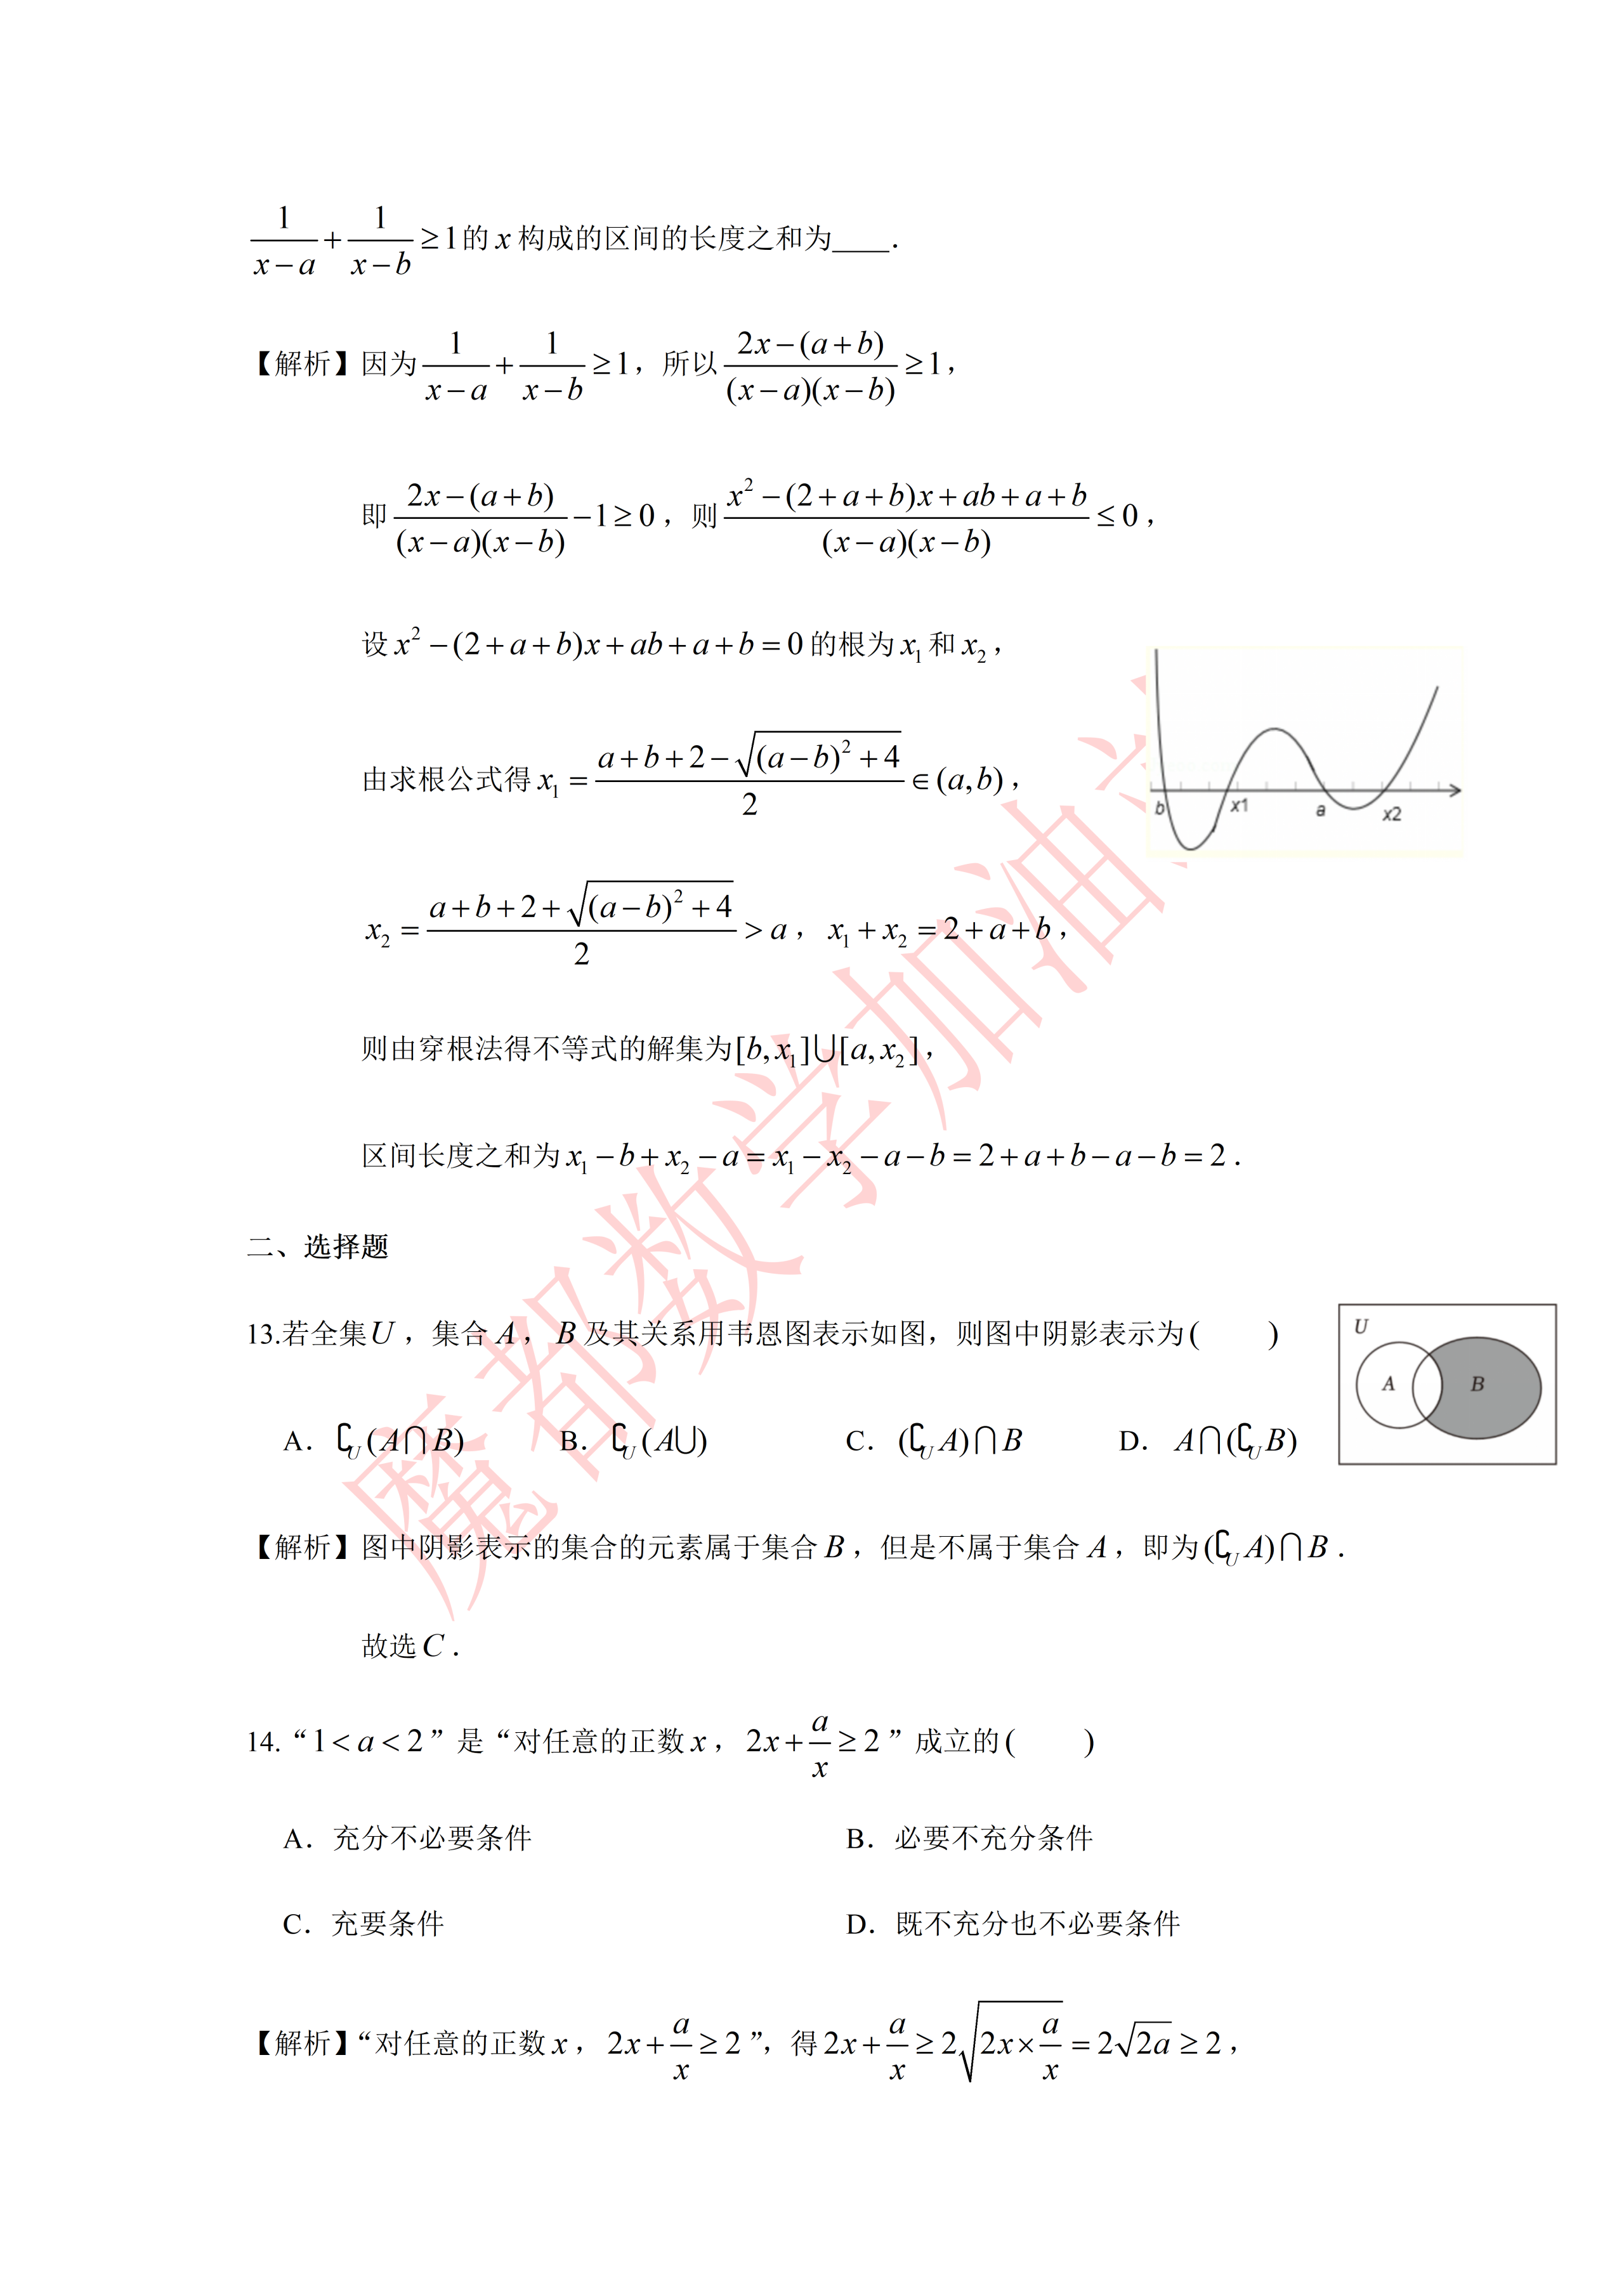
\includegraphics[width=.50\linewidth,trim=1786bp 2255bp 228bp 985bp,clip]{../原图/高一51_华师大二附中_国庆作业3/04.png}
\end{center}
\step{由求根公式得 $x_1=\dfrac{a+b+2-\sqrt{(a-b)^2+4}}{2}\in(a,b)$，}
\step{$x_2=\dfrac{a+b+2+\sqrt{(a-b)^2+4}}{2}>a$，$x_1+x_2=2+a+b$，}
\step{则由穿根法得不等式的解集为 $[b,x_1]\cup[a,x_2]$，}
% 原卷如此，照录未改（此处原卷作 $x_1-x_2$，按上一行 $x_1+x_2=2+a+b$ 当为 $x_1+x_2$）
\step{区间长度之和为 $x_1-b+x_2-a=x_1-x_2-a-b=2+a+b-a-b=2$.}
\solend

\fi

\end{enumerate}

\bigsec{二、选择题}

\begin{enumerate}
\setcounter{enumi}{12}

% 本题是“题干 + 图 + 选项”约 5.5cm 的一整块，图夹在题干与选项之间时 \keepwithprev 挡不住断点，
% 故按 高一30 第 13 题的成例在题前先量一次页高（守卫放在 \item 之前）。
\needvspace{6cm}
\item 若全集 $U$，集合 $A$、$B$ 及其关系用韦恩图表示如图，则图中阴影表示为\mbox{（\quad）}

\begin{center}
% 原卷该图印在题干与选项右侧（原图第 04 页），本稿移作居中排，直接裁取原图，不另存图片文件。
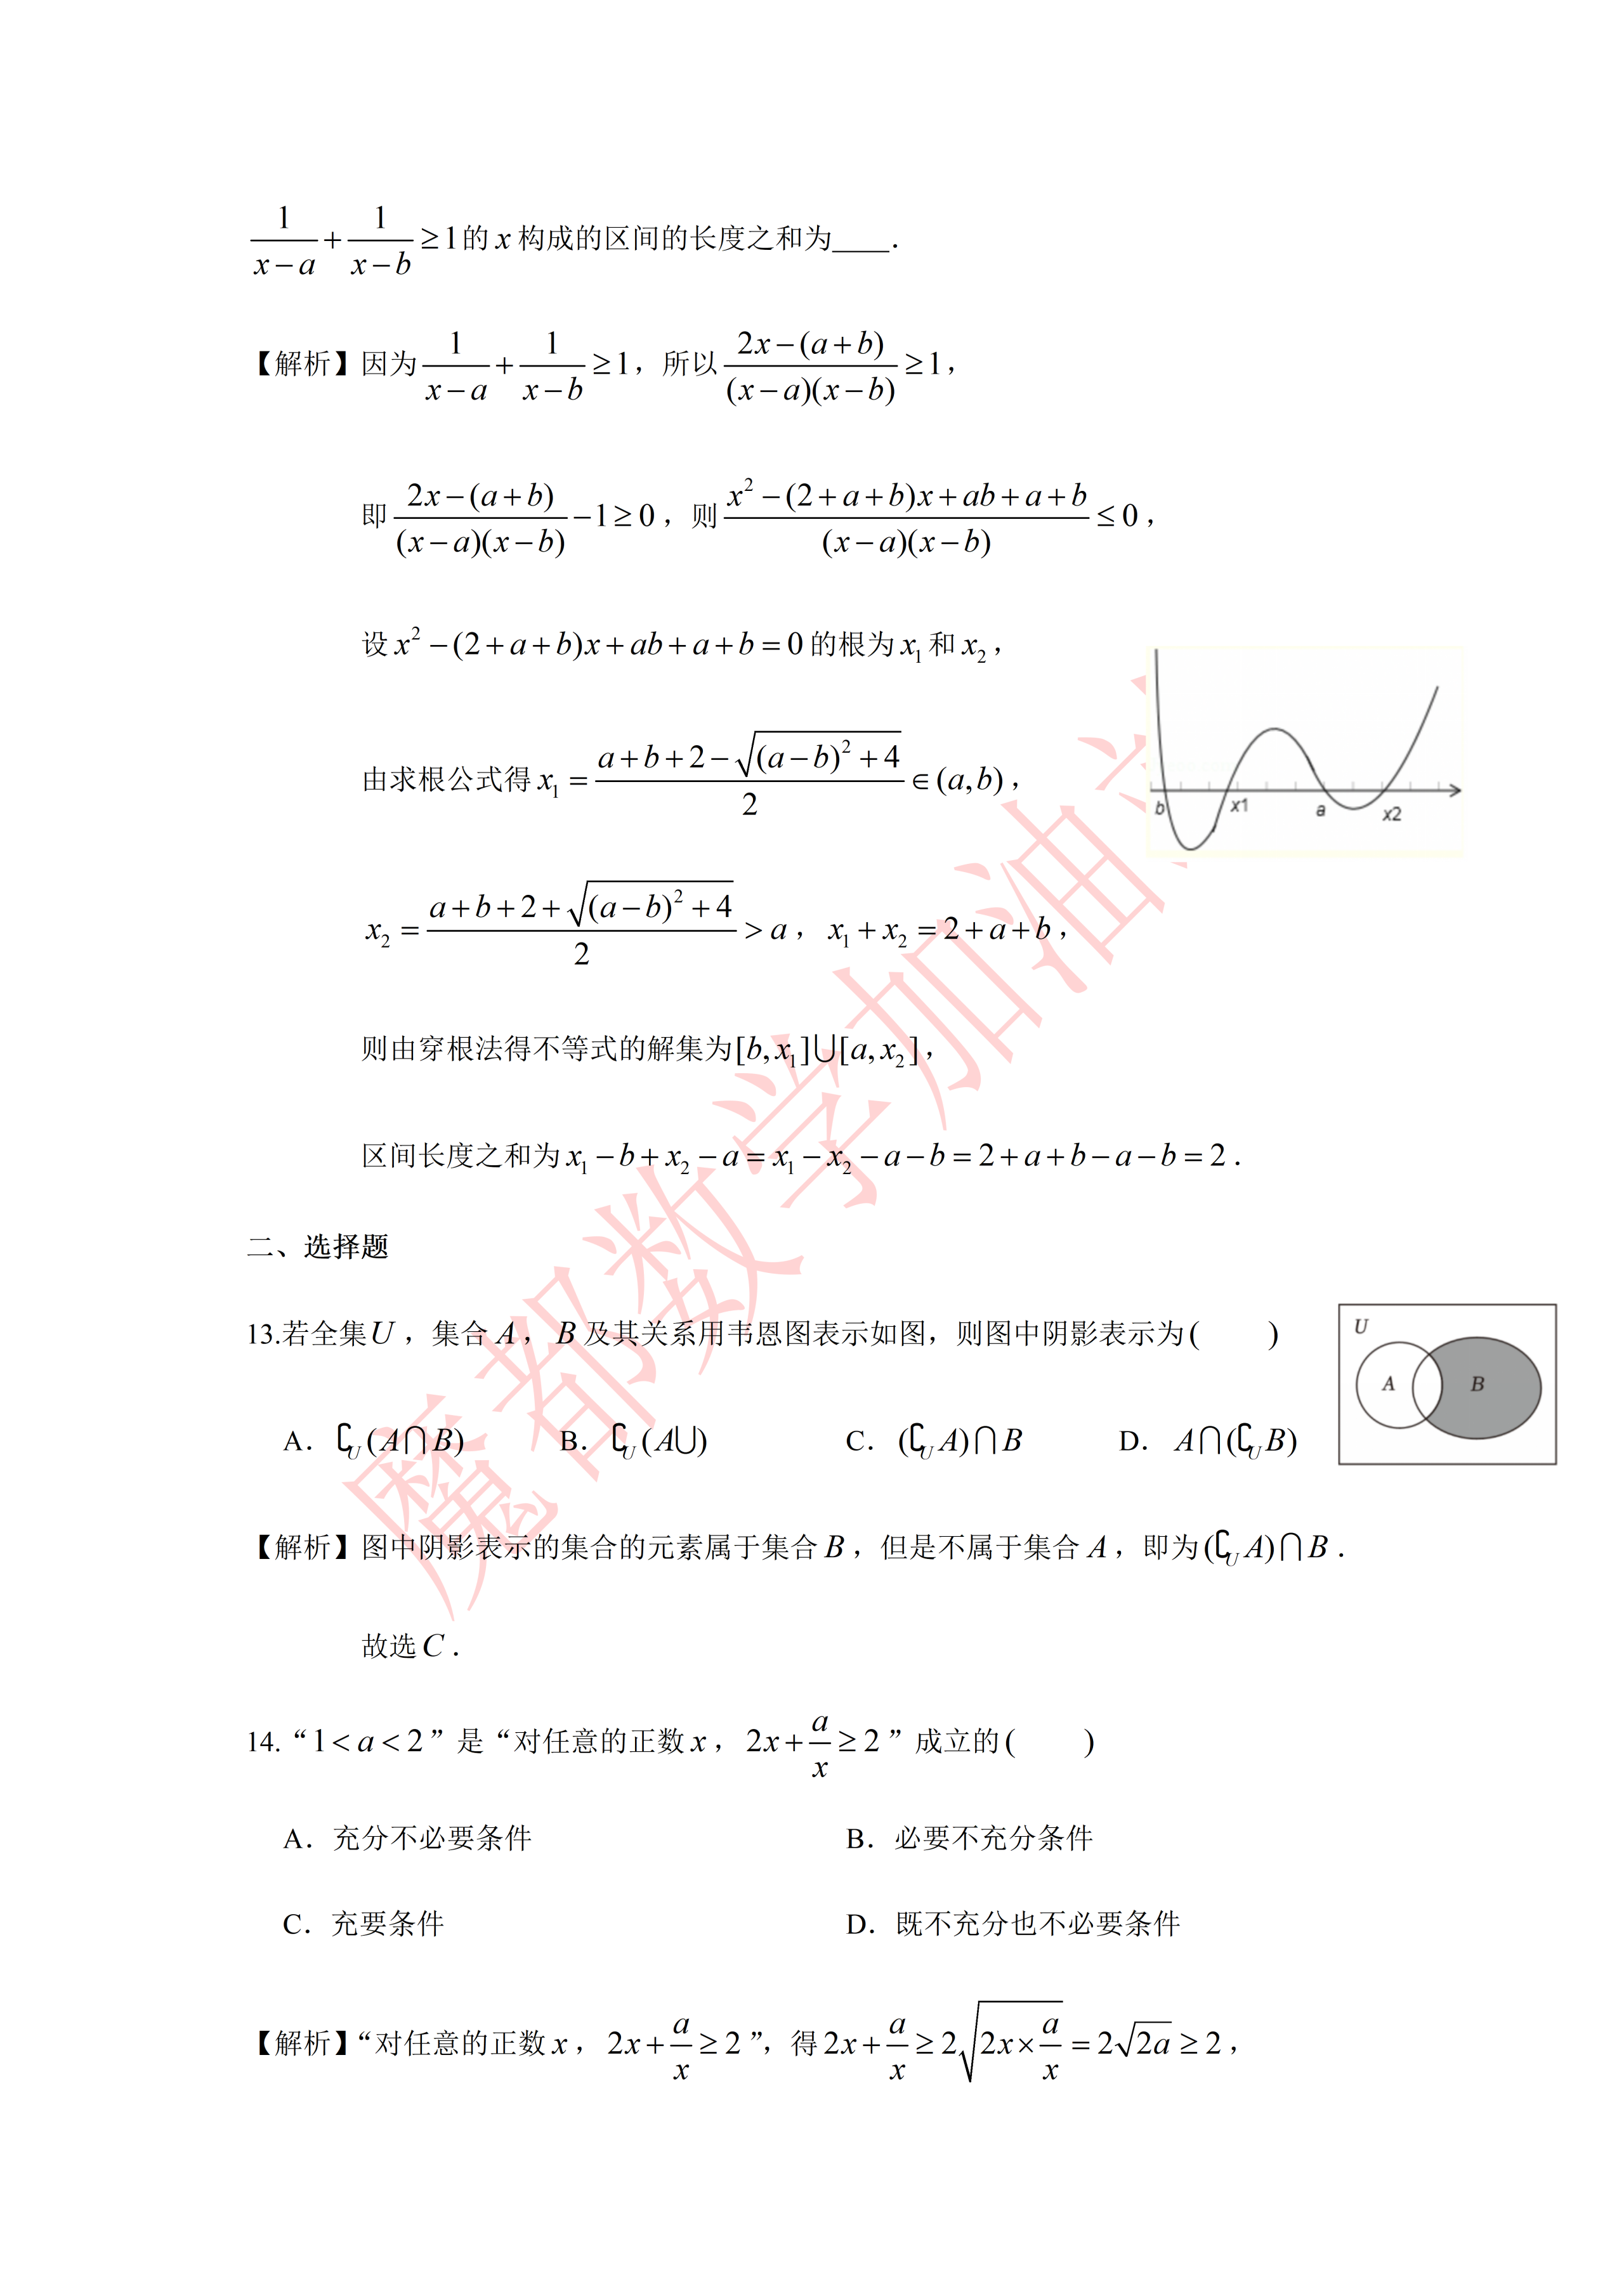
\includegraphics[width=.30\linewidth,trim=2105bp 1308bp 105bp 2050bp,clip]{../原图/高一51_华师大二附中_国庆作业3/04.png}
\end{center}

\keepwithprev
A. $\complement_U(A\cap B)$\qquad B. $\complement_U(A\cup B)$

C. $(\complement_U A)\cap B$\qquad D. $A\cap(\complement_U B)$

\ifanswer
\solbegin
\step{图中阴影表示的集合的元素属于集合 $B$，但是不属于集合 $A$，即为 $(\complement_U A)\cap B$.}
\step{故选 $C$.}
\solend

\fi

\item “$1<a<2$”是“对任意的正数 $x$，$2x+\dfrac ax\geqslant2$”成立的\mbox{（\quad）}

\keepwithprev
A. 充分不必要条件\qquad B. 必要不充分条件

C. 充要条件\qquad\qquad D. 既不充分也不必要条件

\ifanswer
\solbegin
\step{“对任意的正数 $x$，$2x+\dfrac ax\geqslant2$”，得 $2x+\dfrac ax\geqslant2\sqrt{2x\times\dfrac ax}=2\sqrt{2a}\geqslant2$，}
\step{所以 $\sqrt{2a}\geqslant1$，解得 $a\geqslant\dfrac12$，}
\step{若“$1<a<2$”得 $2x+\dfrac ax\geqslant2\sqrt{2x\times\dfrac ax}=2\sqrt{2a}>2\sqrt2>2$，}
\step{所以“$1<a<2$”$\Rightarrow$“对任意的正数 $x$，$2x+\dfrac ax\geqslant2$”，}
\step{所以“$1<a<2$”是“对任意的正数 $x$，$2x+\dfrac ax\geqslant2$”成立的充分不必要条件，}
\step{故选 $A$.}
\solend

\fi

\item 已知函数 $f(x)=2x-3$，$x\in(0,2)$，实数 $a$、$b$ 满足 $f(a)+f(b-1)=0$，则以下成立的有\mbox{（\quad）}

\keepwithprev
A. $a(b-1)$ 的最大值为 $\dfrac94$\qquad\qquad B. $b-\dfrac1a$ 的最大值为 $2$

C. $\dfrac1a+\dfrac1{4b}$ 的最小值为 $\dfrac9{16}$\qquad D. $-1<b-a<3$

\ifanswer
\solbegin
\step{因为函数 $f(x)=2x-3$，$x\in(0,2)$，实数 $a$、$b$ 满足 $f(a)+f(b-1)=0$，}
\step{所以 $2a-3+2(b-1)-3=0$，得 $a+b=4$，$a\in(0,2)$，$b\in(1,3)$，}
\step{所以 $a(b-1)=a(3-a)=-\left(a-\dfrac32\right)^2+\dfrac94$，$a\in(0,2)$，}
\step{所以 $0<a(b-1)\leqslant\dfrac94$，故选项 $A$ 正确；}
\step{$b-\dfrac1a=4-a-\dfrac1a=4-\left(a+\dfrac1a\right)\leqslant4-2=2$，}
\step{当且仅当 $a=1$，$b=3$ 时取等号，又 $b\in(1,3)$，故 $b-\dfrac1a<2$，故 $B$ 错误；}
\step{$\dfrac1a+\dfrac1{4b}=\dfrac14\left(\dfrac1a+\dfrac1{4b}\right)(a+b)=\dfrac14\left(1+\dfrac14+\dfrac ba+\dfrac a{4b}\right)=\dfrac5{16}+\dfrac14\left(\dfrac ba+\dfrac a{4b}\right)$}
\step{$\geqslant\dfrac5{16}+\dfrac14\cdot2\sqrt{\dfrac ba\cdot\dfrac a{4b}}=\dfrac9{16}$，当且仅当 $\dfrac ba=\dfrac a{4b}$，即 $a=2b=\dfrac83$ 时取等号，}
% 原卷如此，照录未改（“又 $a\in(0,2)$，”与下式之间原卷正文夹印“水印”二字）
\step{又 $a\in(0,2)$，水印 $\dfrac1a+\dfrac1{4b}<\dfrac9{16}$，故 $C$ 错误；}
\step{因为 $a\in(0,2)$，$b\in(1,3)$，所以 $-a\in(-2,0)$，所以 $b-a\in(-1,3)$，}
\step{故 $D$ 正确；}
\step{故选 $AD$.}
\solend

\fi

% 本题解析含图（“函数 f(x) 的图像如下”），图夹在解析行间，页末放不下会被拆开，
% 故在题前先量一次页高；上界取“题干 + 选项 + 图 + 首行解析”一块的高度。
\needvspace{6cm}
\item 设 $M_I$ 表示函数 $f(x)=|x^2-4x+2|$ 在闭区间 $I$ 上的最大值. 若正实数 $a$ 满足
$M_{[0,a]}\geqslant2M_{[a,2a]}$，则正实数 $a$ 的取值范围是\mbox{（\quad）}

\keepwithprev
A. $\left[2-\sqrt3,\dfrac12\right]$\qquad B. $[2-\sqrt3,1]$

C. $[2,2+\sqrt3]$\qquad\qquad D. $[2+\sqrt3,4]$

\ifanswer
\solbegin
\step{函数 $f(x)$ 的图像如下：}
\begin{center}
% 原卷该图印在解析行间（原图第 06 页），本稿直接裁取原图，不另存图片文件。
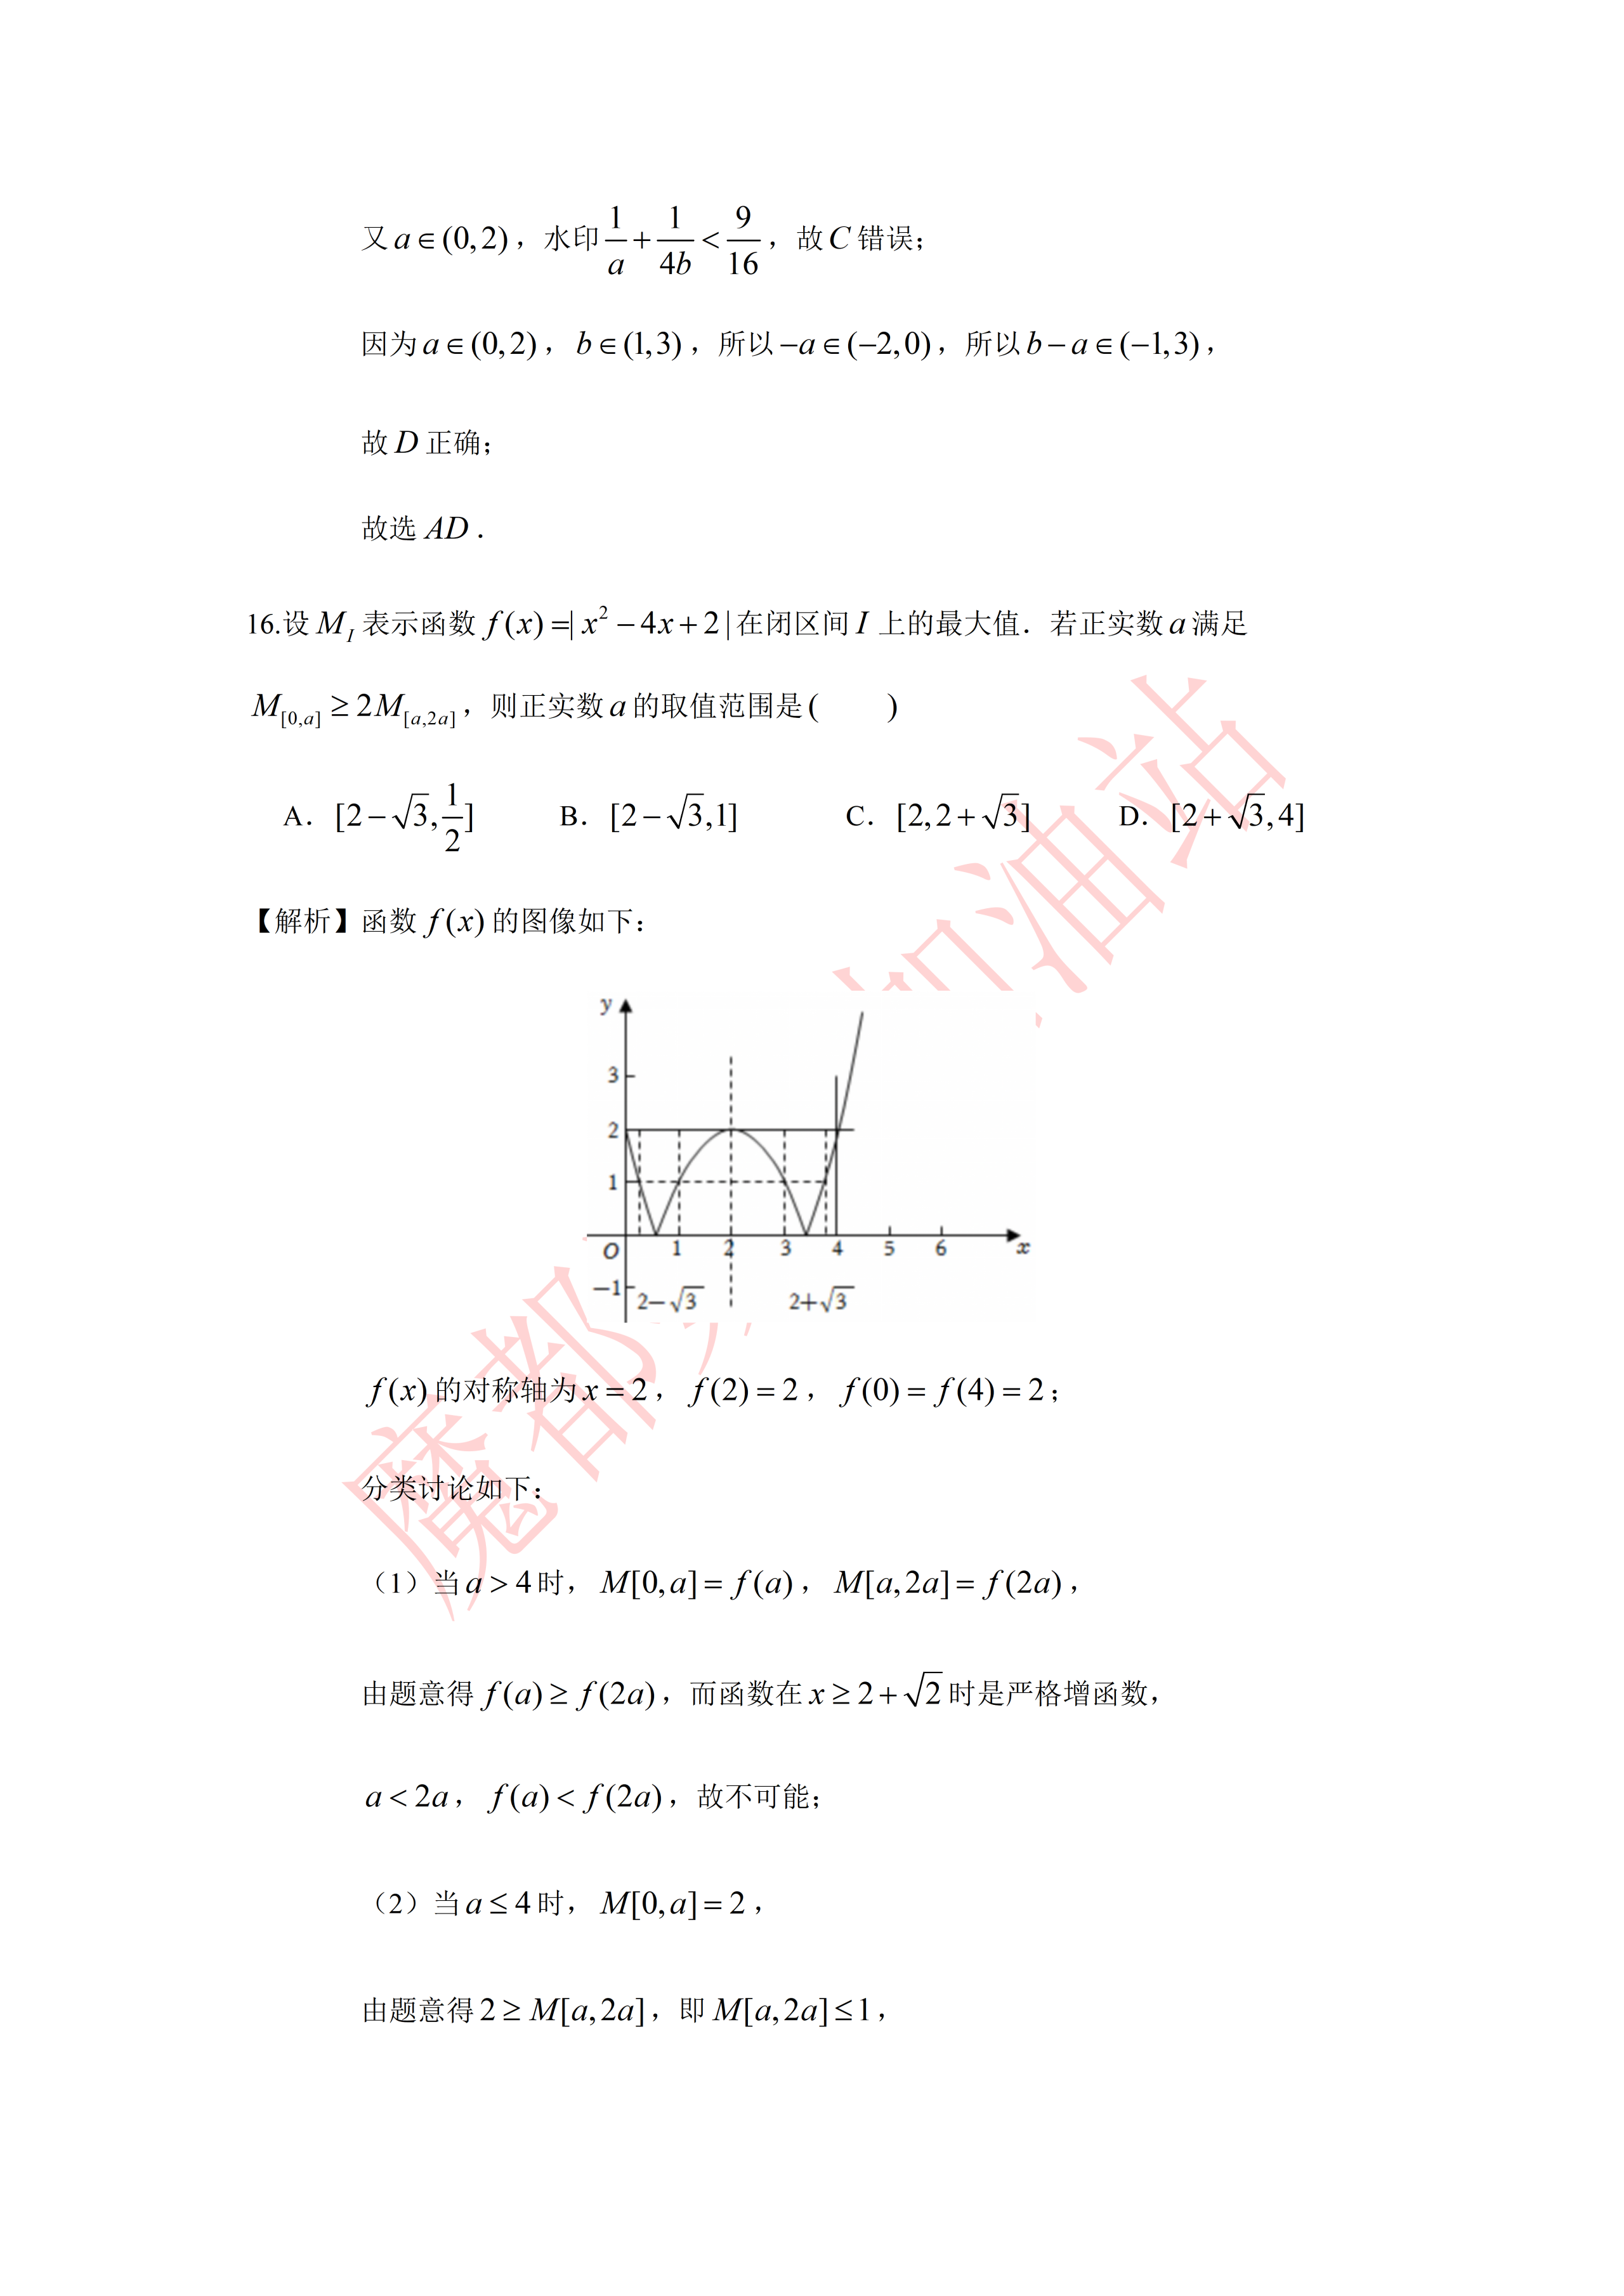
\includegraphics[width=.55\linewidth,trim=895bp 1535bp 915bp 1525bp,clip]{../原图/高一51_华师大二附中_国庆作业3/06.png}
\end{center}
\step{$f(x)$ 的对称轴为 $x=2$，$f(2)=2$，$f(0)=f(4)=2$；}
\step{分类讨论如下：}
\stepm{(1)}{当 $a>4$ 时，$M_{[0,a]}=f(a)$，$M_{[a,2a]}=f(2a)$，}
\step{由题意得 $f(a)\geqslant f(2a)$，而函数在 $x\geqslant2+\sqrt2$ 时是严格增函数，}
\step{$a<2a$，$f(a)<f(2a)$，故不可能；}
\stepm{(2)}{当 $a\leqslant4$ 时，$M_{[0,a]}=2$，}
\step{由题意得 $2\geqslant M_{[a,2a]}$，即 $M_{[a,2a]}\leqslant1$，}
\step{令 $f(x)=1$，解得 $x_1=2-\sqrt3$，$x_2=1$，$x_3=2+\sqrt3$，$x_4=3$，}
\step{则有 $a\geqslant2-\sqrt3$ 并且 $2a\leqslant1$，解得 $2-\sqrt3\leqslant a\leqslant\dfrac12$；}
\step{或者 $a\geqslant3$ 并且 $2a\leqslant2+\sqrt3$，无解；}
\step{故选 $A$.}
\solend

\fi

\end{enumerate}

\bigsec{三、解答题}

\begin{enumerate}
\setcounter{enumi}{16}

\item 已知 $M=\{x\mid2\leqslant x\leqslant5\}$，$N=\{x\mid a-1\leqslant x\leqslant2a+1\}$.
\begin{enumerate}[label=(\arabic*)]
\item 若 $M\subseteq N$，求实数 $a$ 的取值范围；
\item 若 $M\supseteq N$，求实数 $a$ 的取值范围.
\end{enumerate}

\ifanswer
\ans{（1）$[2,3]$；（2）$(-\infty,-2)$}
\fi

\ansspace[6]

\item 设集合 $A=\{x\mid|x+1|\leqslant3\}$，$B=\{x\mid0<x<3m\}$.
\begin{enumerate}[label=(\arabic*)]
\item 若 $A\cup B=A$，求实数 $m$ 的取值范围；
\item 设 $P=(\complement_R A)\cap B$，若 $\exists x\in\Z$ 且 $x\in P$，求实数 $m$ 的取值范围.
\end{enumerate}

\ifanswer
\solbegin
\stepm{(1)}{$A=\{x\mid|x+1|\leqslant3\}=\{x\mid-4\leqslant x\leqslant2\}$，且 $A\cup B=A$，所以 $B\subseteq A$.}
\step{若 $B=\varnothing$，此时 $0\geqslant3m$，解得 $m\leqslant0$；}
\step{若 $B\neq\varnothing$，此时 $0<3m$，且 $3m\leqslant2$，解得 $0<m\leqslant\dfrac23$；}
\step{则实数 $m$ 的取值范围是 $\left(-\infty,\dfrac23\right]$.}
\stepm{(2)}{因为 $\exists x\in\Z$ 且 $x\in P$，所以集合 $P$ 中至少存在一个整数.}
\step{$\complement_R A=\{x\mid x<-4\text{ 或 }x>2\}$，$B=\{x\mid0<x<3m\}$，}
\step{要使 $P=(\complement_R A)\cap B$ 中至少存在一个整数，则 $\begin{cases}3m>0\\3m>3\end{cases}$，解得 $m>1$，}
\step{则实数 $m$ 的取值范围是 $(1,+\infty)$.}
\solend

\fi

\ansspace[7]

\item 已知函数 $f(x)=x^2+(1-a)x-a(a\in\R)$.
\begin{enumerate}[label=(\arabic*)]
\item 解关于 $x$ 的不等式 $f(x)<0$；
\item 若 $\forall a\in[-1,1]$，$f(x)\geqslant0$ 恒成立，求实数 $x$ 的取值范围.
\end{enumerate}

\ifanswer
\solbegin
\stepm{(1)}{不等式 $x^2+(1-a)x-a<0$ 等价于 $(x-a)(x+1)<0$，}
\step{当 $a<-1$ 时，不等式的解集为 $(a,-1)$；}
\step{当 $a=-1$ 时，不等式的解集为 $\varnothing$；}
\step{当 $a>-1$ 时，不等式的解集为 $(-1,a)$.}
\stepm{(2)}{$x^2+(1-a)x-a=-a(x+1)+x^2+x$，}
\step{设 $g(a)=-a(x+1)+x^2+x$，$a\in[-1,1]$，}
\step{要使 $g(a)\geqslant0$ 在 $a\in[-1,1]$ 上恒成立，}
\step{只需 $\begin{cases}g(-1)\geqslant0\\g(1)\geqslant0\end{cases}$，即 $\begin{cases}x^2+2x+1\geqslant0\\x^2-1\geqslant0\end{cases}$，解得 $x\geqslant1$ 或 $x\leqslant-1$，}
\step{所以 $x$ 的取值范围为 $\{x\mid x\leqslant-1\text{ 或 }x\geqslant1\}$.}
\solend

\fi

\ansspace[7]

\item 若实数 $x$、$y$、$m$ 满足 $|x-m|>|y-m|$，则称 $x$ 比 $y$ 远离 $m$.
\begin{enumerate}[label=(\arabic*)]
\item 若 $2$ 比 $3x-4$ 远离 $1$，求 $x$ 的取值范围；
\item 设 $y=\dfrac{x+2}{x+1}$，其中 $x\in(0,\sqrt2)\cup(\sqrt2,+\infty)$，判断：$x$ 与 $y$ 哪一个更远离 $\sqrt2$？并说明理由.
\item 若 $x+y=2$，试问：$y$ 与 $x^2+y^2$ 哪一个更远离 $\dfrac12$？并说明理由.
\end{enumerate}

\ifanswer
\solbegin
\stepm{(1)}{由题意得 $|2-1|>|3x-4-1|$，所以 $|3x-5|<1$，解得 $\dfrac43<x<2$，}
\step{故 $x$ 的取值范围为 $\left(\dfrac43,2\right)$；}
\stepm{(2)}{$x$ 比 $y$ 更远离 $\sqrt2$，}
\step{理由如下：要证 $x$ 比 $y$ 更远离 $\sqrt2$，只要证 $|x-\sqrt2|>\left|\dfrac{x+2}{x+1}-\sqrt2\right|$，}
\step{即证 $|x-\sqrt2|>\left|\dfrac{(1-\sqrt2)(x-\sqrt2)}{x+1}\right|$，}
\step{因为 $x\in(0,\sqrt2)\cup(\sqrt2,+\infty)$，所以 $|x-\sqrt2|>0$，}
\step{所以只要证 $1>\dfrac{\sqrt2-1}{|x+1|}$，即证 $|x+1|>\sqrt2-1$，}
\step{因为 $x\in(0,\sqrt2)\cup(\sqrt2,+\infty)$，所以 $x+1\in(1,\sqrt2+1)\cup(\sqrt2+1,+\infty)$，}
\step{所以 $|x+1|>1>\sqrt2-1$，所以 $x$ 比 $y$ 更远离 $\sqrt2$；}
\stepm{(3)}{因为 $x^2+y^2\geqslant\dfrac{(x+y)^2}{2}=2$，当且仅当 $x=y=1$ 时等号成立，}
\step{所以 $\left|x^2+y^2-\dfrac12\right|=x^2+y^2-\dfrac12$，}
\step{从而 $\left|y-\dfrac12\right|-\left|x^2+y^2-\dfrac12\right|=\left|y-\dfrac12\right|-\left(x^2+y^2-\dfrac12\right)$，}
\step{①$y\geqslant\dfrac12$，$\left|y-\dfrac12\right|-\left|x^2+y^2-\dfrac12\right|=y-\dfrac12-\left(x^2+y^2-\dfrac12\right)=y-x^2-y^2$}
\step{$=y-(2-y)^2-y^2=-2y^2+5y-4=-2\left(y-\dfrac54\right)^2-\dfrac78<0$，}
\step{即 $\left|y-\dfrac12\right|<\left|x^2+y^2-\dfrac12\right|$；}
\step{②$y<\dfrac12$，}
\step{$\left|y-\dfrac12\right|-\left|x^2+y^2-\dfrac12\right|=\left(\dfrac12-y\right)-\left(x^2+y^2-\dfrac12\right)=-y-x^2-y^2+1$}
\step{$=-y-(2-y)^2-y^2+1=-2y^2+3y-3=-2\left(y-\dfrac34\right)^2-\dfrac{15}8<0$，}
\step{即 $\left|y-\dfrac12\right|<\left|x^2+y^2-\dfrac12\right|$；}
\step{综上，$\left|y-\dfrac12\right|<\left|x^2+y^2-\dfrac12\right|$，即 $x^2+y^2$ 比 $y$ 更远离 $\dfrac12$.}
\solend

\fi

\ansspace[9]

\item 对于非空有限整数集 $X$，$m\in\N^*$，定义 $X^m=\{x^m\mid x\in X\}$，对 $n\in\Z$，
$Y\oplus n=\{x+n\mid x\in Y\}$ 现有两个非空有限整数集 $A$、$B$，已知 $A\oplus1\subseteq B$ 且
$B^2\oplus(-4)\subseteq A$.
\begin{enumerate}[label=(\arabic*)]
\item 当 $A=\{-3,0\}$ 时求集合 $B$；
\item 证明：$A\subseteq\{-3,-2,0,1\}$；
\item 当 $A\oplus1=B$ 且 $B^2\oplus(-4)=A$ 时，任取 $a\in A$，$b\in B$ 构造函数
$f(x)=(x-a)(x-b)$ 问：当 $a$、$b$ 取何值时，$f(x)$ 的最小值最小？
\end{enumerate}

\ifanswer
\solbegin
\stepm{(1)}{因为 $A=\{-3,0\}$，$B^2\oplus(-4)\subseteq A$，}
\step{所以 $B^2\oplus(-4)$ 可能为 $\varnothing$、$\{-3\}$、$\{0\}$、$\{-3,0\}$，}
\step{当 $B^2\oplus(-4)=\varnothing$ 时 $B^2=\varnothing$，不满足非空，不合题意；}
\step{当 $B^2\oplus(-4)=\{-3\}$ 时 $B^2=\{1\}$，所以 $B=\{1,-1\}$、$\{1\}$、$\{-1\}$，}
\step{当 $B^2\oplus(-4)=\{0\}$ 时 $B^2=\{4\}$，所以 $B=\{2,-2\}$、$\{2\}$、$\{-2\}$，}
% 原卷如此，照录未改（此处作 $\{0,-3\}$，上一行同一集合作 $\{-3,0\}$）
\step{当 $B^2\oplus(-4)=\{0,-3\}$ 时 $B^2=\{4,1\}$，}
\step{所以 $B=\{1,2,-1,-2\}$、$\{2,-1,-2\}$、$\{2,1,-2\}$、$\{1,-1,-2\}$、$\{1,-1,2\}$、$\{1,2\}$、$\{-1,2\}$、$\{-1,-2\}$、$\{1,-2\}$，}
\step{又 $A\oplus1=\{-2,1\}\subseteq B$，得 $B$ 为 $\{1,-2\}$、$\{2,1,-2\}$、$\{1,-1,-2\}$、$\{1,2,-1,-2\}$.}
\stepm{(2)}{设 $x\in A$，因为 $A\oplus1\subseteq B$，所以 $x+1\in B$，}
\step{又 $B^2\oplus(-4)\subseteq A$，所以 $(x+1)^2-4\in A$，}
% 原卷如此，照录未改（此处及下文取 $x=2$ 处原卷均作 $(-4+1)^2-4=52-2a>0$）
\step{取 $x=-4$，则 $(-4+1)^2-4=52-2a>0$，$(5+1)^2-4=32\in A$，$\cdots$，}
\step{无限迭代，而 $A$ 为有限集，不合题意，舍去，即 $-4\notin A$；}
\step{取 $x=-3$，则 $(-3+1)^2-4=0\in A$，$(0+1)^2-4=-3\in A$，}
\step{得 $A$ 集合可为 $\{-3,0\}$；}
\step{取 $x=-2$，则 $(-2+1)^2-4=-3\in A$，$(-3+1)^2-4=0\in A$，}
\step{$(0+1)^2-4=-3\in A$，得 $A$ 集合可为 $\{-3,-2,0\}$；}
\step{取 $x=-1$，则 $(-1+1)^2-4=-4\in A$，又 $-4\notin A$，所以 $-1\notin A$，}
\step{取 $x=1$，则 $(1+1)^2-4=0\in A$，$(0+1)^2-4=-3\in A$，}
\step{$(-3+1)^2-4=0\in A$，得 $A$ 集合可为 $\{-3,0,1\}$，}
\step{取 $x=2$，则 $(2+1)^2-4=52-2a>0$，$(5+1)^2-4=32\in A$，$\cdots$，}
\step{无限迭代，而 $A$ 为有限集，不合题意，舍去，即 $2\notin A$，}
\step{同理当 $x<-4$ 或 $x>2$，且 $x\in\Z$ 时不符合 $A$ 为有限集，舍去；}
\step{故由上得 $A$ 集合可为 $\{-3,0\},\{-3,-2,0\},\{-3,0,1\},\{-3,-2,0,1\}$，}
\step{所以 $A\subseteq\{-3,-2,0,1\}$，}
\stepm{(3)}{当 $A\oplus1=B$ 且 $B^2\oplus(-4)=A$ 时，}
\step{设 $x\in B$，则 $x^2-4\in B^2\oplus(-4)=A$，}
% 原卷如此，照录未改（题设 $A=\{-3,0\}$，此处两个判别式取的是 $-2$ 与 $1$，均不属于 $A$）
\step{$x^2-4=-2$ 时 $x=\pm\sqrt2$，不为整数，不合题意；}
\step{$x^2-4=1$ 时 $x=\pm\sqrt5$，不为整数，不合题意；}
\step{所以 $A=\{-3,0\}$，又 $A\oplus1=B$，则 $B=\{-2,1\}$，}
\step{任取 $a\in A$，$b\in B$ 构造函数 $f(x)=(x-a)(x-b)$，}
\step{$f(x)=(x-a)(x-b)=x^2-(a+b)x+ab$}
\step{$=x^2-(a+b)x+\dfrac{(a+b)^2}{4}+ab-\dfrac{(a+b)^2}{4}$}
\step{$=\left[x-\dfrac{(a+b)}2\right]^2-\dfrac{(a-b)^2}{4}\geqslant-\dfrac{(a-b)^2}{4}$，所以 $f(x)_{min}=-\dfrac{(a-b)^2}{4}$，}
\step{又 $a\in A=\{-3,0\}$，$b\in B=\{-2,1\}$，所以 $a-b$ 的取值有 $-1,-4,2$，}
\step{所以 $f(x)_{min}=-\dfrac{(a-b)^2}{4}\geqslant-\dfrac{(-3-1)^2}{4}=-4$，}
\step{即当 $a=-3$，$b=1$ 时 $f(x)_{min}$ 的最小值为 $-4$.}
\solend

\fi

\ansspace*[12]

\end{enumerate}

\end{document}
"
% 紧凑版：xelatex "\def\iscompact{1}% 高一51_华师大二附中_国庆作业3.tex
%   —— 高一上数学“2026-2027 年华师大二附中高一上国庆作业 3”（讲评版）
% 试卷版：xelatex 高一51_华师大二附中_国庆作业3.tex
% 答案版：xelatex "\def\isanswer{1}\input{高一51_华师大二附中_国庆作业3.tex}"
% 紧凑版：xelatex "\def\iscompact{1}\input{高一51_华师大二附中_国庆作业3.tex}"
%
% 原始材料：微信公众号“魔都数学加油站”文章，作者破晓，连载“27学年高一51”；
% 原文标题“27学年高一51——2026-2027年上海市华师大二附中高一上国庆作业3”；
% 原文链接：https://mp.weixin.qq.com/s/95SLMEmPUT30s4U7wjr5Og。
% 该页面用 JS 渲染，未见明确发布日期；页面内时间戳约为 2026-10-05 21:37，本稿以该时刻记可得日期。
% 正文为 12 张 PNG 页：第 01、02、03、05、07、08、11 页 4762×6735，
% 第 04、06、09、10、12 页 2560×3620。按页序逐页读取，12 页全为试卷正文页
% （卷首标题在第 1 页页顶，卷末解答题止于第 12 页），无封面页、目录页或单独的页脚页。
% 卷面标题照原卷印作“2026-2027 年华师大二附中高一上国庆作业 3”（公众号标题中的“上海市”
% 卷面标题行没有，本稿照卷面），年份区间按全稿惯例排 en dash。
%
% 篇幅与题号：原卷自第 3 题起编号（第 1、2 题不在本卷内）。填空题 3—12（10 题）、
% 选择题 13—16（4 题）、解答题 17—21（5 题），共 19 题。本稿沿用原节与原题号，
% 只改排为全稿统一的大节样式（原卷小节标题为“一、填空题”“二、选择题”“三、解答题”）。
% 正文为讲评版：填空题 3—12 与选择题 13—16 只印【解析】（选择题的结论“故选 X”印在解析内），
% 按全稿口径这类题不另提 \ans{}；解答题第 17 题只印【答案】，故只给 \ans{}；
% 第 18—21 题只印【解析】。
%
% 副标题：原卷未印副标题。本稿按“知识模块”口径标作“集合与常用逻辑用语、不等式”：
% 19 题中集合与常用逻辑用语 8 题（3、4、6、10、13、17、18、21），
% 不等式（含函数最值、绝对值不等式）11 题（5、7、8、9、11、12、14、15、16、19、20），
% 两类均远超三分之一，故并标。口径同 高一46_交附闵行_国庆作业3、高一48_华师大二附中_周末作业2。
%
% 与原卷的排版差异：
%   ① 原卷每题下直接印【答案】或【解析】，本稿按全稿惯例将答案与解析置于答案版；
%   ② 原卷未印副标题，本稿按“知识模块”口径补出；
%   ③ 原卷填空横线按全稿惯例排为 \blankline[4.4em]；
%   ④ 原卷 $R$、$N$、$Z$ 均排斜体，本稿按全稿惯例改用花体 $\R$、$\N$、$\Z$（同 高一48）；
%   ⑤ 原卷第 12 题解析配图、第 13 题题干韦恩图都印在正文右侧的浮动位置，第 16 题解析配图
%      印在解析行间；本稿三图一律居中排，均自原图对应页裁切（trim），不另存图片文件；
%   ⑥ 原卷解答题未留作答空白，本稿按全稿惯例加 \ansspace；
%   ⑦ 原卷第 15 题解析第 7、8 两个印刷行是一串连等式的折行，本稿按“一条 \step ＝ 一个印刷行”
%      的口径分成两条 \step。
%
% 原卷笔误/存疑（均照录未改，正文对应处另有 % 注）：
%   ① 第 12 题解析末行作“区间长度之和为 $x_1-b+x_2-a=x_1-x_2-a-b=2+a+b-a-b=2$”，
%      按上一行 $x_1+x_2=2+a+b$，此处应为 $x_1+x_2$；原卷作 $x_1-x_2$。
%   ② 第 15 题解析“又 $a\in(0,2)$，”与 $\dfrac1a+\dfrac1{4b}<\dfrac9{16}$ 之间，
%      原卷正文夹印“水印”二字（系制版遗留字样，非试卷内容）。
%   ③ 第 21 题第 (2) 问解析两处（取 $x=-4$、取 $x=2$）作“$=52-2a>0$”，
%      与题设 $(x+1)^2-4$ 的取值（按 $x=-4$ 应为 $5$）不符，当系原卷算式遗留。
%   ④ 第 21 题第 (1) 问解析先写 $B^2\oplus(-4)$ 可能为 $\{-3,0\}$，后文又作 $\{0,-3\}$，
%      同一集合两种写法。
%   ⑤ 第 21 题第 (3) 问解析：题设 $B^2\oplus(-4)=A$ 且 $A=\{-3,0\}$ 时，由 $x^2-4\in A$
%      应得 $x^2-4=-3$ 或 $0$；原卷讨论的却是 $x^2-4=-2$ 与 $x^2-4=1$（两值均不属于 $A$），
%      与题设不合。
%
% 插图：3 张，均自原图裁切（无 \begin{tikzpicture} 重排）：
%   · 第 13 题题干韦恩图（原图第 04 页，图在题干与选项右侧）
%   · 第 12 题解析配图（原图第 04 页，图在解析右侧）
%   · 第 16 题解析配图（原图第 06 页，图在解析中间）
%
\documentclass[a4paper,11pt]{article}
\usepackage{common}

\begin{document}

\examtitlest[3]{2026--2027 年华师大二附中高一上国庆作业 3}{集合与常用逻辑用语、不等式}

\bigsec{一、填空题}

\begin{enumerate}
\setcounter{enumi}{2}

\item 若 $\{x\mid x<1\text{ 或 }x>4\}\cup\{x\mid m<x<2m+3\}=R$，则实数 $m$ 的取值范围为\blankline[4.4em].

\ifanswer
\solbegin
\step{因为 $\{x\mid x<1\text{ 或 }x>4\}\cup\{x\mid m<x<2m+3\}=R$，}
\step{所以 $\begin{cases}m<1\\2m+3>4\end{cases}$，解得 $\dfrac12<m<1$，所以 $m$ 的取值范围为 $\left(\dfrac12,1\right)$.}
\solend

\fi

\item 若“$x\leqslant5$”是“$x<a$”的必要不充分条件，则 $a$ 的取值范围是\blankline[4.4em].

\ifanswer
\solbegin
\step{若“$x\leqslant5$”是“$x<a$”的必要不充分条件，则 $\{x\mid x<a\}\subset\{x\mid x\leqslant5\}$，}
\step{所以 $a\leqslant5$.}
\solend

\fi

\item 实数 $x$、$y$ 满足 $x^2+2xy+4y^2=1$，则 $x+2y$ 的取值范围是\blankline[4.4em].

\ifanswer
\solbegin
\step{因为 $x^2+2xy+4y^2=(x+2y)^2-2xy=1$，}
\step{所以 $(x+2y)^2-1=x\cdot(2y)\leqslant\left(\dfrac{x+2y}{2}\right)^2$，当且仅当 $x=2y$ 时取等号，}
\step{解得 $-\dfrac{2\sqrt3}{3}\leqslant x+2y\leqslant\dfrac{2\sqrt3}{3}$，故 $x+2y$ 的取值范围是 $\left[-\dfrac{2\sqrt3}{3},\dfrac{2\sqrt3}{3}\right]$.}
\solend

\fi

\item 若命题 $p$：“$\exists x\in\R$，$5x^2-3x+m=0$”为假命题，则实数 $m$ 的取值范围为\blankline[4.4em].

\ifanswer
\solbegin
\step{若命题 $p$：$\exists x\in\R$，$5x^2-3x+m=0$ 为假命题，}
\step{则 $5x^2-3x+m=0$ 没有实数根，故 $\Delta=9-20m<0$，解得 $m>\dfrac9{20}$.}
\solend

\fi

\item 若当 $3\leqslant m\leqslant5$ 时，$mx^2-mx+m-9<0$ 有解，则实数 $x$ 的取值范围是\blankline[4.4em].

\ifanswer
\solbegin
\step{当 $3\leqslant m\leqslant5$ 时，$mx^2-mx+m-9<0$ 有解，}
\step{即 $(x^2-x+1)m-9<0$ 在 $m\in[3,5]$ 上有解，}
\step{因为 $x^2-x+1>0$，所以一次函数 $g(m)=(x^2-x+1)m-9$ 严格增，}
\step{所以只需 $g(3)=3x^2-3x-6<0$ 即可，}
\step{即 $x^2-x-2<0$，$(x-2)(x+1)<0$，解得 $-1<x<2$，}
\step{所以实数 $x$ 的取值范围是 $(-1,2)$.}
\solend

\fi

\item 已知不等式 $\dfrac{x}{x^2+4}\leqslant a$ 对任意的 $x\in[1,3]$ 恒成立，则实数 $a$ 的范围为\blankline[4.4em].

\ifanswer
\solbegin
\step{因为 $x\in[1,3]$，所以 $\dfrac{x}{x^2+4}=\dfrac{1}{x+\dfrac4x}\leqslant\dfrac{1}{2\sqrt{x\times\dfrac4x}}=\dfrac14$，}
\step{当且仅当 $x=\dfrac4x$ 时，即 $x=2$ 时取等号，即 $\dfrac{x}{x^2+4}$ 在 $x\in[1,3]$ 的最大值为 $\dfrac14$，}
\step{又由不等式 $\dfrac{x}{x^2+4}\leqslant a$ 对任意的 $x\in[1,3]$ 恒成立，所以 $a\geqslant\dfrac14$，}
\step{即实数 $a$ 的范围为 $\left[\dfrac14,+\infty\right)$.}
\solend

\fi

\item 甲、乙两人解关于 $x$ 的不等式 $x^2+bx+c<0$，甲写错了 $b$，正确计算后得到的解为 $\{x\mid1<x<2\}$；
乙写错了 $c$，正确计算后得到的解为 $\{x\mid-4<x<1\}$. 那么不等式 $\dfrac{bx+c}{x-2}<0$ 的解为\blankline[4.4em].

\ifanswer
\solbegin
\step{由 $x^2+bx+c<0$ 的解为 $\{x\mid1<x<2\}$，}
\step{则 $1$ 和 $2$ 是方程 $x^2+bx+c=0$ 的两个根，}
\step{甲写错了 $b$，但 $c$ 是正确的，所以 $c=1\times2=2$；}
\step{由 $x^2+bx+c<0$ 的解为 $\{x\mid-4<x<1\}$，}
\step{则 $-4$ 和 $1$ 是方程 $x^2+bx+c=0$ 的两个根，}
\step{乙写错了 $c$，但 $b$ 是正确的，所以 $-b=-4+1=-3$，即 $b=3$.}
\step{由 $\dfrac{bx+c}{x-2}<0$，得 $\dfrac{3x+2}{x-2}<0$，即 $(3x+2)(x-2)<0$，解得 $-\dfrac23<x<2$.}
\step{不等式 $\dfrac{bx+c}{x-2}<0$ 的解为 $\left\{x\mid-\dfrac23<x<2\right\}$.}
\solend

\fi

\item 已知 $\dfrac{1}{x-2}\geqslant1$ 是 $|x-a|<2$ 的充分非必要条件，则实数 $a$ 的取值范围是\blankline[4.4em].

\ifanswer
\solbegin
\step{由 $\dfrac{1}{x-2}\geqslant1$ 得 $\dfrac{3-x}{x-2}\geqslant0$，解得 $2<x\leqslant3$，由 $|x-a|<2$ 得 $a-2<x<a+2$，}
\step{因为 $\dfrac{1}{x-2}\geqslant1$ 是 $|x-a|<2$ 的充分非必要条件，}
\step{所以 $\{x\mid2<x\leqslant3\}\subset\{x\mid a-2<x<a+2\}$，所以 $\begin{cases}a-2\leqslant2\\a+2>3\end{cases}$，解得 $1<a\leqslant4$，}
\step{即实数 $a$ 的取值范围是 $(1,4]$.}
\solend

\fi

\item 设 $a>0$，$b>0$，若不等式 $a(a+1)^2+b(b+1)^2\geqslant\lambda ab$ 恒成立，则实数 $\lambda$ 的最大值为\blankline[4.4em].

\ifanswer
\solbegin
\step{$a(a+1)^2+b(b+1)^2\geqslant\lambda ab\Leftrightarrow\lambda\leqslant\dfrac{a(a+1)^2+b(b+1)^2}{ab}=\dfrac{(a+1)^2}{b}+\dfrac{(b+1)^2}{a}$，}
\step{从而原问题转化为求 $\dfrac{(a+1)^2}{b}+\dfrac{(b+1)^2}{a}$ 的最小值.}
\step{因为 $\dfrac{(a+1)^2}{b}+\dfrac{(b+1)^2}{a}=\dfrac{b^2+2b+1}{a}+\dfrac{a^2+2a+1}{b}$}
\step{$=\left(\dfrac{b^2}{a}+\dfrac{a^2}{b}\right)+2\left(\dfrac ba+\dfrac ab\right)+\left(\dfrac1a+\dfrac1b\right)\geqslant2\sqrt{\dfrac{b^2}{a}\cdot\dfrac{a^2}{b}}+2\times2\sqrt{\dfrac ba\cdot\dfrac ab}+2\sqrt{\dfrac1a\cdot\dfrac1b}$}
\step{$=2\sqrt{ab}+4+\dfrac{2}{\sqrt{ab}}\geqslant2\sqrt{2\sqrt{ab}\cdot\dfrac{2}{\sqrt{ab}}}+4=8$，以上均当且仅当 $a=b$ 时取等号，}
\step{所以 $\lambda\leqslant8$，即实数 $\lambda$ 的最大值为 $8$.}
\solend

\fi

\item 定义区间 $(a,d)$、$[a,d)$、$(a,d]$、$[a,d]$ 的长度为 $d-a$（$d>a$），已知 $a>b$，则满足
$\dfrac{1}{x-a}+\dfrac{1}{x-b}\geqslant1$ 的 $x$ 构成的区间的长度之和为\blankline[4.4em].

\ifanswer
\solbegin
\step{因为 $\dfrac{1}{x-a}+\dfrac{1}{x-b}\geqslant1$，所以 $\dfrac{2x-(a+b)}{(x-a)(x-b)}\geqslant1$，}
\step{即 $\dfrac{2x-(a+b)}{(x-a)(x-b)}-1\geqslant0$，则 $\dfrac{x^2-(2+a+b)x+ab+a+b}{(x-a)(x-b)}\leqslant0$，}
\step{设 $x^2-(2+a+b)x+ab+a+b=0$ 的根为 $x_1$ 和 $x_2$，}
\begin{center}
% 原卷该图印在解析右侧（原图第 04 页），本稿移作居中排，直接裁取原图，不另存图片文件。
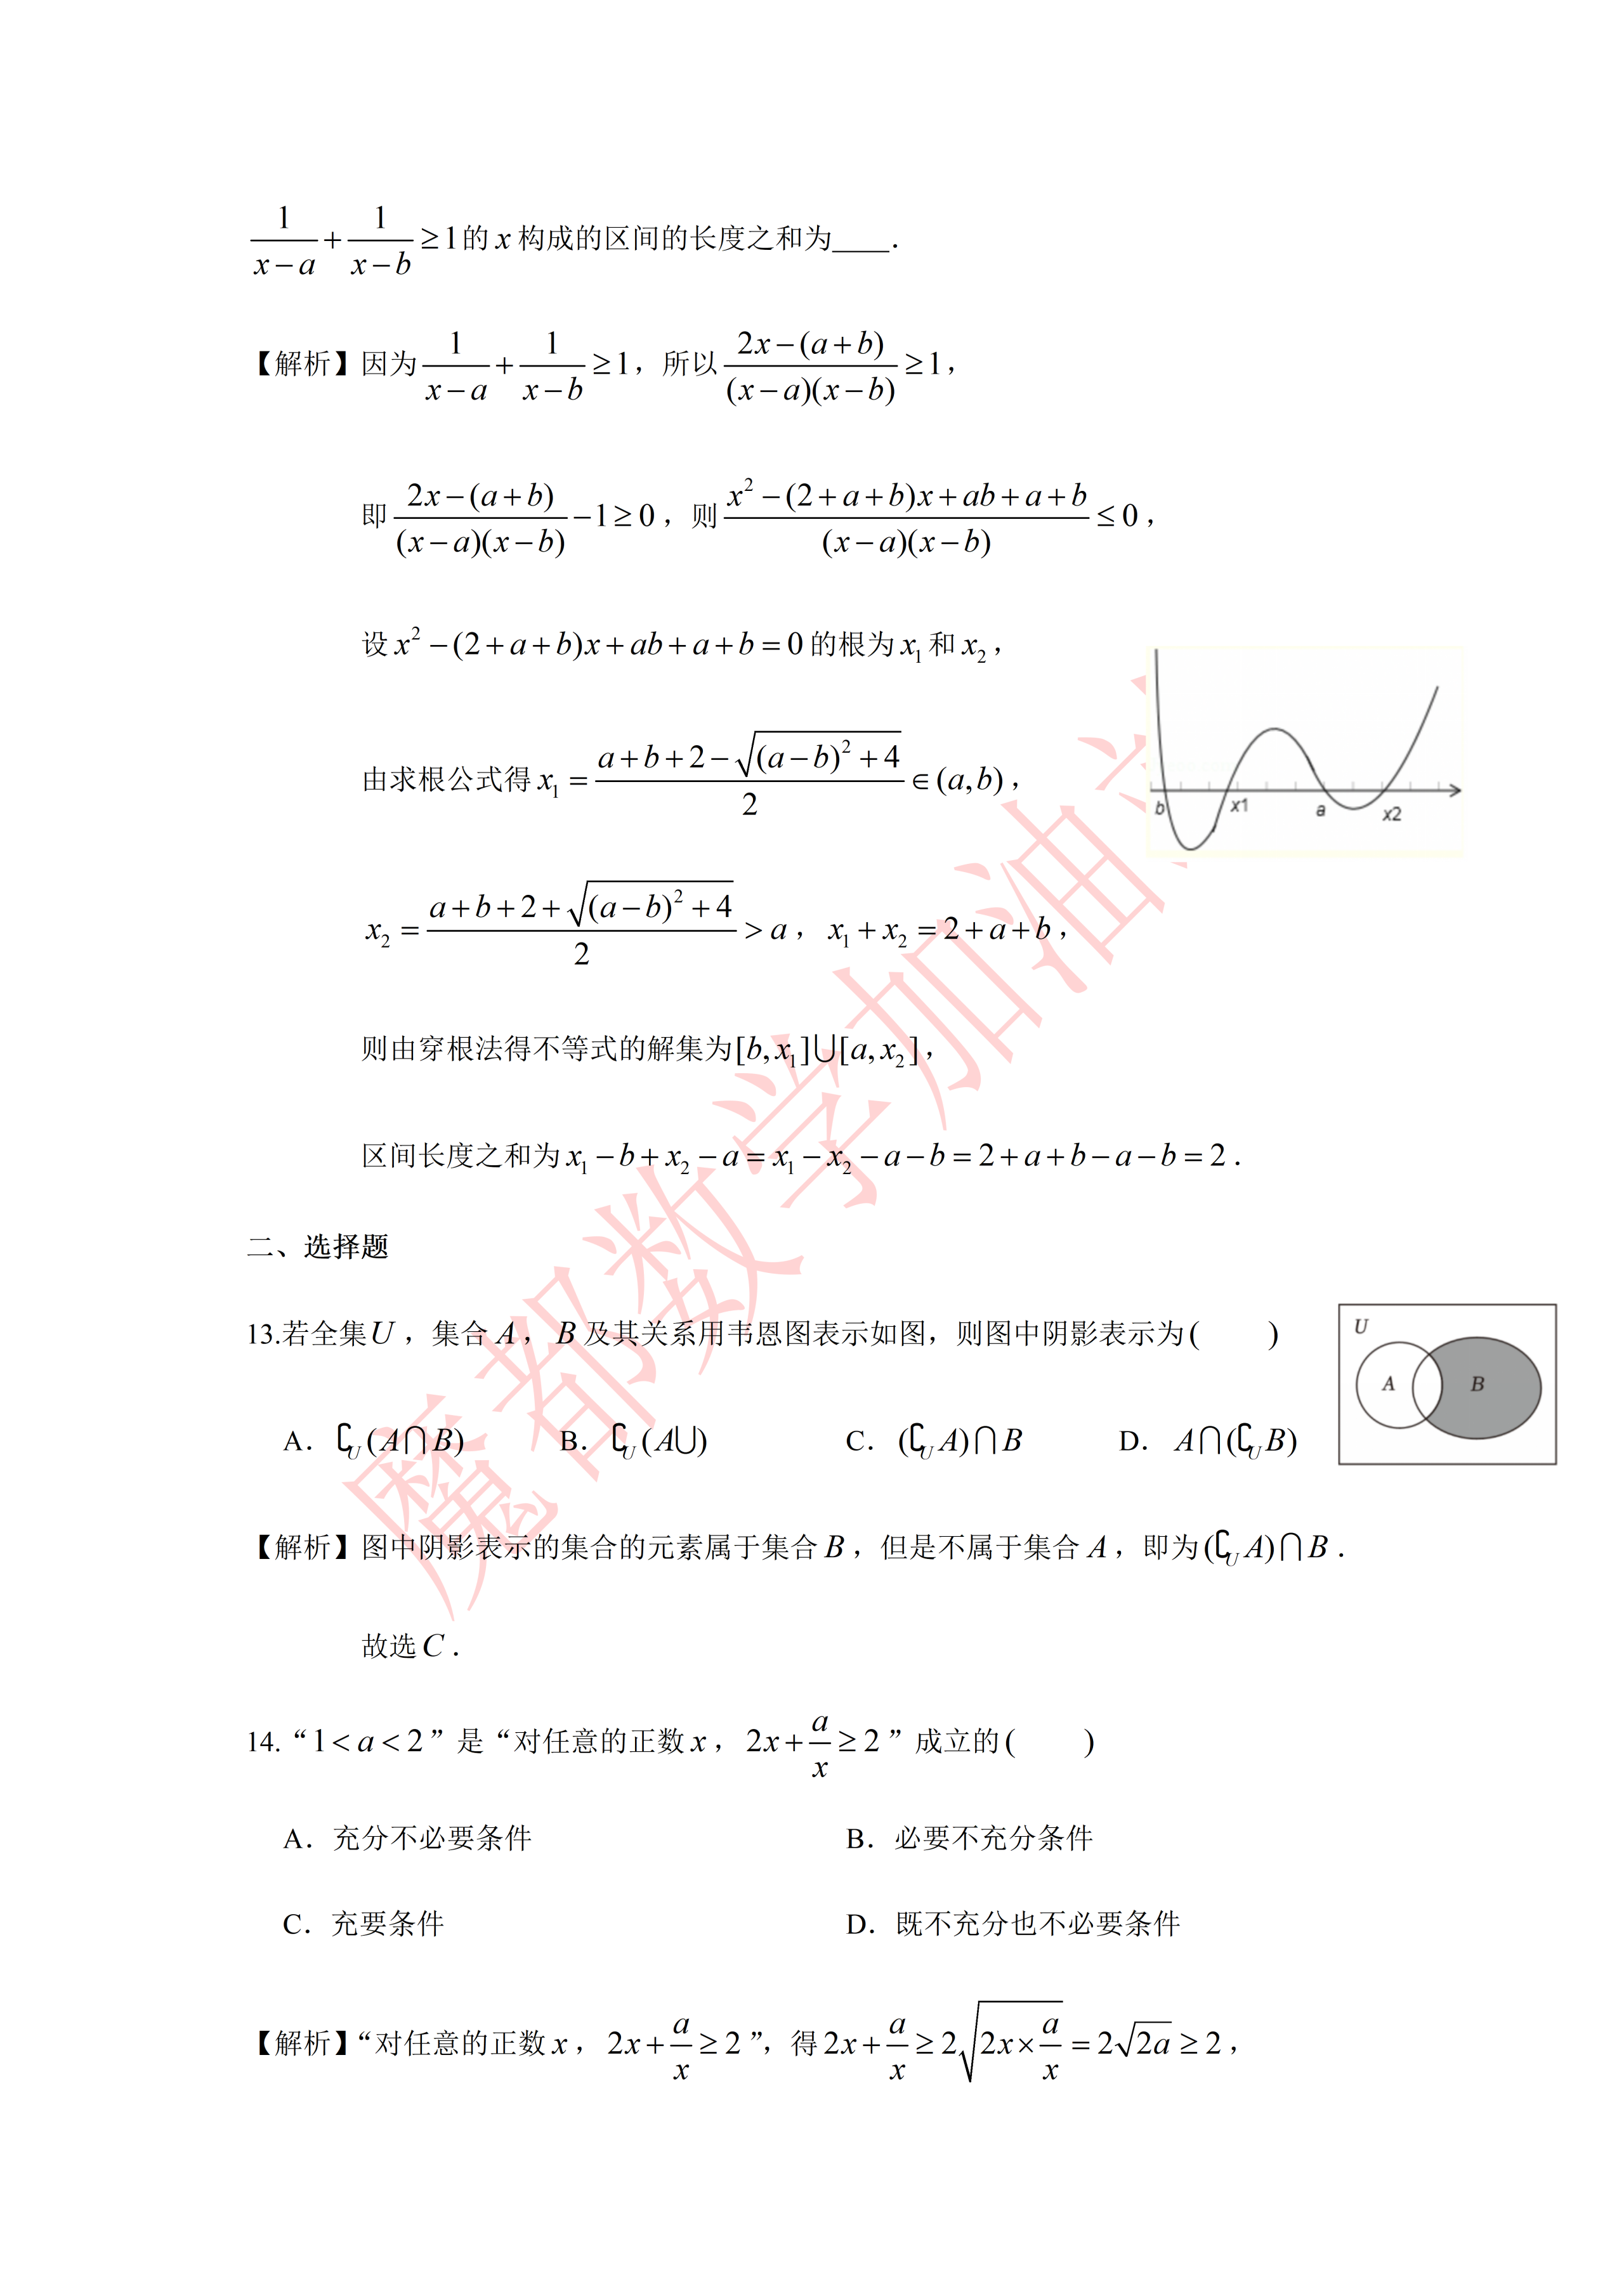
\includegraphics[width=.50\linewidth,trim=1786bp 2255bp 228bp 985bp,clip]{../原图/高一51_华师大二附中_国庆作业3/04.png}
\end{center}
\step{由求根公式得 $x_1=\dfrac{a+b+2-\sqrt{(a-b)^2+4}}{2}\in(a,b)$，}
\step{$x_2=\dfrac{a+b+2+\sqrt{(a-b)^2+4}}{2}>a$，$x_1+x_2=2+a+b$，}
\step{则由穿根法得不等式的解集为 $[b,x_1]\cup[a,x_2]$，}
% 原卷如此，照录未改（此处原卷作 $x_1-x_2$，按上一行 $x_1+x_2=2+a+b$ 当为 $x_1+x_2$）
\step{区间长度之和为 $x_1-b+x_2-a=x_1-x_2-a-b=2+a+b-a-b=2$.}
\solend

\fi

\end{enumerate}

\bigsec{二、选择题}

\begin{enumerate}
\setcounter{enumi}{12}

% 本题是“题干 + 图 + 选项”约 5.5cm 的一整块，图夹在题干与选项之间时 \keepwithprev 挡不住断点，
% 故按 高一30 第 13 题的成例在题前先量一次页高（守卫放在 \item 之前）。
\needvspace{6cm}
\item 若全集 $U$，集合 $A$、$B$ 及其关系用韦恩图表示如图，则图中阴影表示为\mbox{（\quad）}

\begin{center}
% 原卷该图印在题干与选项右侧（原图第 04 页），本稿移作居中排，直接裁取原图，不另存图片文件。
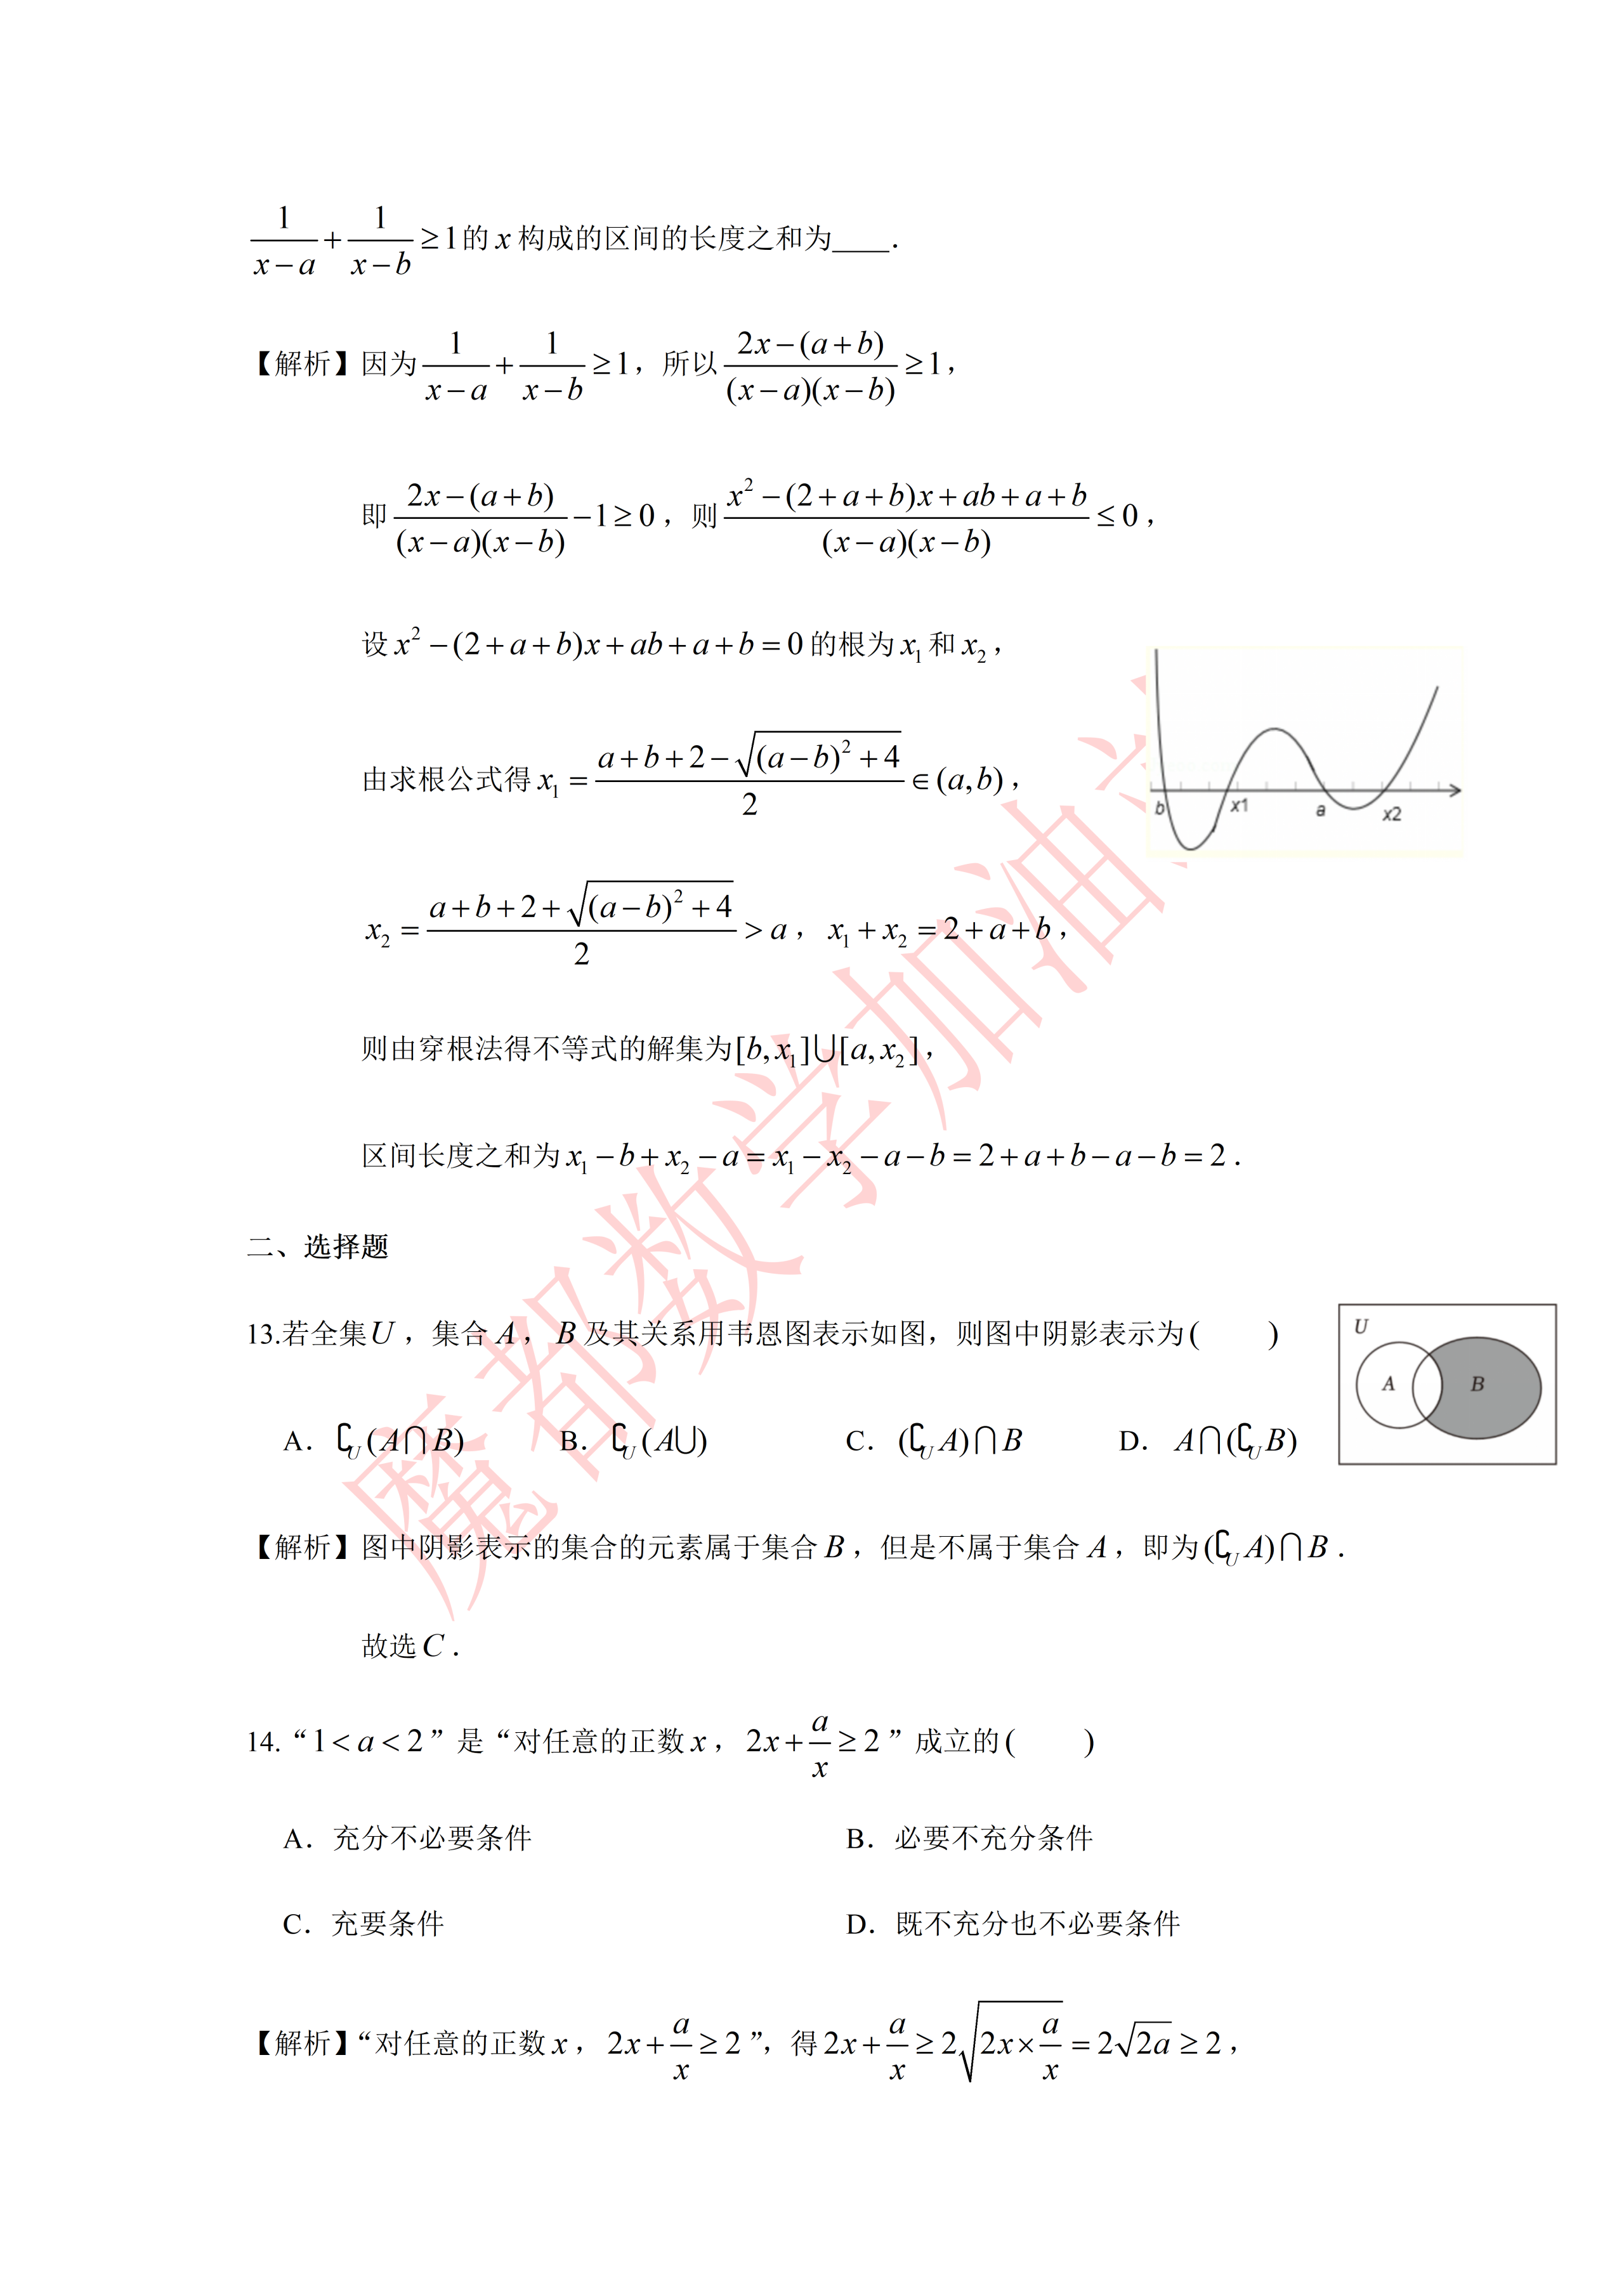
\includegraphics[width=.30\linewidth,trim=2105bp 1308bp 105bp 2050bp,clip]{../原图/高一51_华师大二附中_国庆作业3/04.png}
\end{center}

\keepwithprev
A. $\complement_U(A\cap B)$\qquad B. $\complement_U(A\cup B)$

C. $(\complement_U A)\cap B$\qquad D. $A\cap(\complement_U B)$

\ifanswer
\solbegin
\step{图中阴影表示的集合的元素属于集合 $B$，但是不属于集合 $A$，即为 $(\complement_U A)\cap B$.}
\step{故选 $C$.}
\solend

\fi

\item “$1<a<2$”是“对任意的正数 $x$，$2x+\dfrac ax\geqslant2$”成立的\mbox{（\quad）}

\keepwithprev
A. 充分不必要条件\qquad B. 必要不充分条件

C. 充要条件\qquad\qquad D. 既不充分也不必要条件

\ifanswer
\solbegin
\step{“对任意的正数 $x$，$2x+\dfrac ax\geqslant2$”，得 $2x+\dfrac ax\geqslant2\sqrt{2x\times\dfrac ax}=2\sqrt{2a}\geqslant2$，}
\step{所以 $\sqrt{2a}\geqslant1$，解得 $a\geqslant\dfrac12$，}
\step{若“$1<a<2$”得 $2x+\dfrac ax\geqslant2\sqrt{2x\times\dfrac ax}=2\sqrt{2a}>2\sqrt2>2$，}
\step{所以“$1<a<2$”$\Rightarrow$“对任意的正数 $x$，$2x+\dfrac ax\geqslant2$”，}
\step{所以“$1<a<2$”是“对任意的正数 $x$，$2x+\dfrac ax\geqslant2$”成立的充分不必要条件，}
\step{故选 $A$.}
\solend

\fi

\item 已知函数 $f(x)=2x-3$，$x\in(0,2)$，实数 $a$、$b$ 满足 $f(a)+f(b-1)=0$，则以下成立的有\mbox{（\quad）}

\keepwithprev
A. $a(b-1)$ 的最大值为 $\dfrac94$\qquad\qquad B. $b-\dfrac1a$ 的最大值为 $2$

C. $\dfrac1a+\dfrac1{4b}$ 的最小值为 $\dfrac9{16}$\qquad D. $-1<b-a<3$

\ifanswer
\solbegin
\step{因为函数 $f(x)=2x-3$，$x\in(0,2)$，实数 $a$、$b$ 满足 $f(a)+f(b-1)=0$，}
\step{所以 $2a-3+2(b-1)-3=0$，得 $a+b=4$，$a\in(0,2)$，$b\in(1,3)$，}
\step{所以 $a(b-1)=a(3-a)=-\left(a-\dfrac32\right)^2+\dfrac94$，$a\in(0,2)$，}
\step{所以 $0<a(b-1)\leqslant\dfrac94$，故选项 $A$ 正确；}
\step{$b-\dfrac1a=4-a-\dfrac1a=4-\left(a+\dfrac1a\right)\leqslant4-2=2$，}
\step{当且仅当 $a=1$，$b=3$ 时取等号，又 $b\in(1,3)$，故 $b-\dfrac1a<2$，故 $B$ 错误；}
\step{$\dfrac1a+\dfrac1{4b}=\dfrac14\left(\dfrac1a+\dfrac1{4b}\right)(a+b)=\dfrac14\left(1+\dfrac14+\dfrac ba+\dfrac a{4b}\right)=\dfrac5{16}+\dfrac14\left(\dfrac ba+\dfrac a{4b}\right)$}
\step{$\geqslant\dfrac5{16}+\dfrac14\cdot2\sqrt{\dfrac ba\cdot\dfrac a{4b}}=\dfrac9{16}$，当且仅当 $\dfrac ba=\dfrac a{4b}$，即 $a=2b=\dfrac83$ 时取等号，}
% 原卷如此，照录未改（“又 $a\in(0,2)$，”与下式之间原卷正文夹印“水印”二字）
\step{又 $a\in(0,2)$，水印 $\dfrac1a+\dfrac1{4b}<\dfrac9{16}$，故 $C$ 错误；}
\step{因为 $a\in(0,2)$，$b\in(1,3)$，所以 $-a\in(-2,0)$，所以 $b-a\in(-1,3)$，}
\step{故 $D$ 正确；}
\step{故选 $AD$.}
\solend

\fi

% 本题解析含图（“函数 f(x) 的图像如下”），图夹在解析行间，页末放不下会被拆开，
% 故在题前先量一次页高；上界取“题干 + 选项 + 图 + 首行解析”一块的高度。
\needvspace{6cm}
\item 设 $M_I$ 表示函数 $f(x)=|x^2-4x+2|$ 在闭区间 $I$ 上的最大值. 若正实数 $a$ 满足
$M_{[0,a]}\geqslant2M_{[a,2a]}$，则正实数 $a$ 的取值范围是\mbox{（\quad）}

\keepwithprev
A. $\left[2-\sqrt3,\dfrac12\right]$\qquad B. $[2-\sqrt3,1]$

C. $[2,2+\sqrt3]$\qquad\qquad D. $[2+\sqrt3,4]$

\ifanswer
\solbegin
\step{函数 $f(x)$ 的图像如下：}
\begin{center}
% 原卷该图印在解析行间（原图第 06 页），本稿直接裁取原图，不另存图片文件。
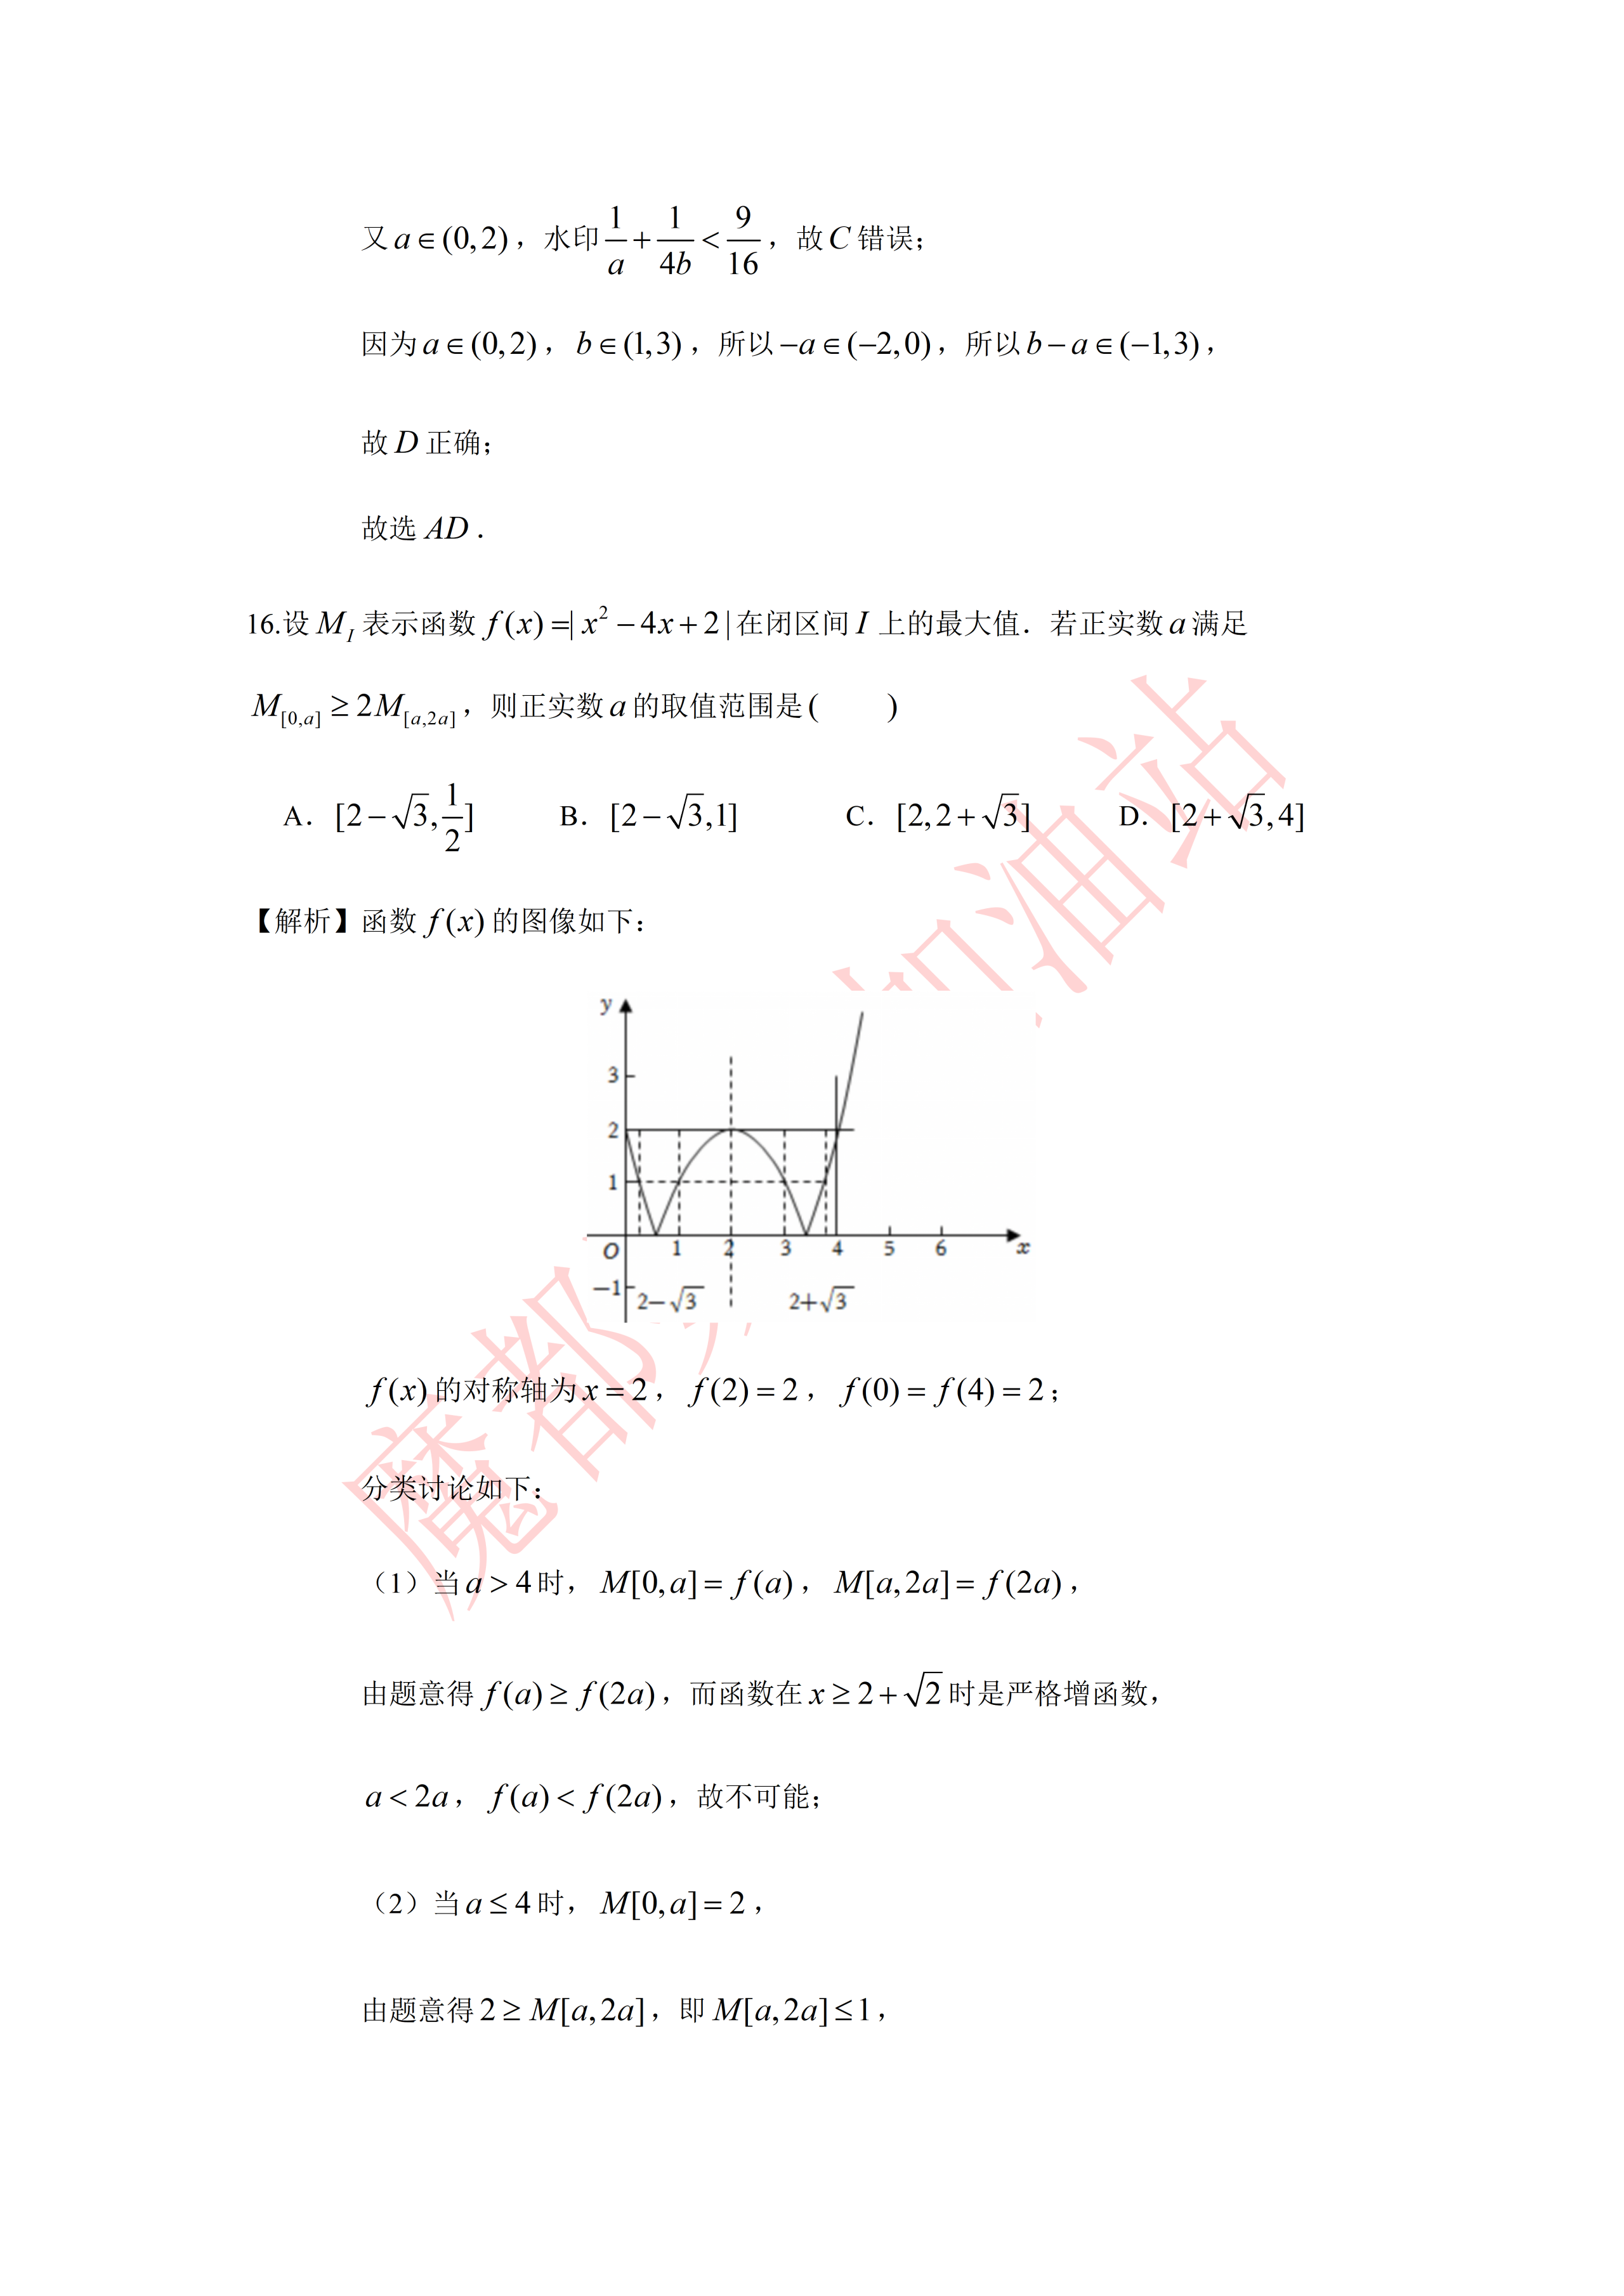
\includegraphics[width=.55\linewidth,trim=895bp 1535bp 915bp 1525bp,clip]{../原图/高一51_华师大二附中_国庆作业3/06.png}
\end{center}
\step{$f(x)$ 的对称轴为 $x=2$，$f(2)=2$，$f(0)=f(4)=2$；}
\step{分类讨论如下：}
\stepm{(1)}{当 $a>4$ 时，$M_{[0,a]}=f(a)$，$M_{[a,2a]}=f(2a)$，}
\step{由题意得 $f(a)\geqslant f(2a)$，而函数在 $x\geqslant2+\sqrt2$ 时是严格增函数，}
\step{$a<2a$，$f(a)<f(2a)$，故不可能；}
\stepm{(2)}{当 $a\leqslant4$ 时，$M_{[0,a]}=2$，}
\step{由题意得 $2\geqslant M_{[a,2a]}$，即 $M_{[a,2a]}\leqslant1$，}
\step{令 $f(x)=1$，解得 $x_1=2-\sqrt3$，$x_2=1$，$x_3=2+\sqrt3$，$x_4=3$，}
\step{则有 $a\geqslant2-\sqrt3$ 并且 $2a\leqslant1$，解得 $2-\sqrt3\leqslant a\leqslant\dfrac12$；}
\step{或者 $a\geqslant3$ 并且 $2a\leqslant2+\sqrt3$，无解；}
\step{故选 $A$.}
\solend

\fi

\end{enumerate}

\bigsec{三、解答题}

\begin{enumerate}
\setcounter{enumi}{16}

\item 已知 $M=\{x\mid2\leqslant x\leqslant5\}$，$N=\{x\mid a-1\leqslant x\leqslant2a+1\}$.
\begin{enumerate}[label=(\arabic*)]
\item 若 $M\subseteq N$，求实数 $a$ 的取值范围；
\item 若 $M\supseteq N$，求实数 $a$ 的取值范围.
\end{enumerate}

\ifanswer
\ans{（1）$[2,3]$；（2）$(-\infty,-2)$}
\fi

\ansspace[6]

\item 设集合 $A=\{x\mid|x+1|\leqslant3\}$，$B=\{x\mid0<x<3m\}$.
\begin{enumerate}[label=(\arabic*)]
\item 若 $A\cup B=A$，求实数 $m$ 的取值范围；
\item 设 $P=(\complement_R A)\cap B$，若 $\exists x\in\Z$ 且 $x\in P$，求实数 $m$ 的取值范围.
\end{enumerate}

\ifanswer
\solbegin
\stepm{(1)}{$A=\{x\mid|x+1|\leqslant3\}=\{x\mid-4\leqslant x\leqslant2\}$，且 $A\cup B=A$，所以 $B\subseteq A$.}
\step{若 $B=\varnothing$，此时 $0\geqslant3m$，解得 $m\leqslant0$；}
\step{若 $B\neq\varnothing$，此时 $0<3m$，且 $3m\leqslant2$，解得 $0<m\leqslant\dfrac23$；}
\step{则实数 $m$ 的取值范围是 $\left(-\infty,\dfrac23\right]$.}
\stepm{(2)}{因为 $\exists x\in\Z$ 且 $x\in P$，所以集合 $P$ 中至少存在一个整数.}
\step{$\complement_R A=\{x\mid x<-4\text{ 或 }x>2\}$，$B=\{x\mid0<x<3m\}$，}
\step{要使 $P=(\complement_R A)\cap B$ 中至少存在一个整数，则 $\begin{cases}3m>0\\3m>3\end{cases}$，解得 $m>1$，}
\step{则实数 $m$ 的取值范围是 $(1,+\infty)$.}
\solend

\fi

\ansspace[7]

\item 已知函数 $f(x)=x^2+(1-a)x-a(a\in\R)$.
\begin{enumerate}[label=(\arabic*)]
\item 解关于 $x$ 的不等式 $f(x)<0$；
\item 若 $\forall a\in[-1,1]$，$f(x)\geqslant0$ 恒成立，求实数 $x$ 的取值范围.
\end{enumerate}

\ifanswer
\solbegin
\stepm{(1)}{不等式 $x^2+(1-a)x-a<0$ 等价于 $(x-a)(x+1)<0$，}
\step{当 $a<-1$ 时，不等式的解集为 $(a,-1)$；}
\step{当 $a=-1$ 时，不等式的解集为 $\varnothing$；}
\step{当 $a>-1$ 时，不等式的解集为 $(-1,a)$.}
\stepm{(2)}{$x^2+(1-a)x-a=-a(x+1)+x^2+x$，}
\step{设 $g(a)=-a(x+1)+x^2+x$，$a\in[-1,1]$，}
\step{要使 $g(a)\geqslant0$ 在 $a\in[-1,1]$ 上恒成立，}
\step{只需 $\begin{cases}g(-1)\geqslant0\\g(1)\geqslant0\end{cases}$，即 $\begin{cases}x^2+2x+1\geqslant0\\x^2-1\geqslant0\end{cases}$，解得 $x\geqslant1$ 或 $x\leqslant-1$，}
\step{所以 $x$ 的取值范围为 $\{x\mid x\leqslant-1\text{ 或 }x\geqslant1\}$.}
\solend

\fi

\ansspace[7]

\item 若实数 $x$、$y$、$m$ 满足 $|x-m|>|y-m|$，则称 $x$ 比 $y$ 远离 $m$.
\begin{enumerate}[label=(\arabic*)]
\item 若 $2$ 比 $3x-4$ 远离 $1$，求 $x$ 的取值范围；
\item 设 $y=\dfrac{x+2}{x+1}$，其中 $x\in(0,\sqrt2)\cup(\sqrt2,+\infty)$，判断：$x$ 与 $y$ 哪一个更远离 $\sqrt2$？并说明理由.
\item 若 $x+y=2$，试问：$y$ 与 $x^2+y^2$ 哪一个更远离 $\dfrac12$？并说明理由.
\end{enumerate}

\ifanswer
\solbegin
\stepm{(1)}{由题意得 $|2-1|>|3x-4-1|$，所以 $|3x-5|<1$，解得 $\dfrac43<x<2$，}
\step{故 $x$ 的取值范围为 $\left(\dfrac43,2\right)$；}
\stepm{(2)}{$x$ 比 $y$ 更远离 $\sqrt2$，}
\step{理由如下：要证 $x$ 比 $y$ 更远离 $\sqrt2$，只要证 $|x-\sqrt2|>\left|\dfrac{x+2}{x+1}-\sqrt2\right|$，}
\step{即证 $|x-\sqrt2|>\left|\dfrac{(1-\sqrt2)(x-\sqrt2)}{x+1}\right|$，}
\step{因为 $x\in(0,\sqrt2)\cup(\sqrt2,+\infty)$，所以 $|x-\sqrt2|>0$，}
\step{所以只要证 $1>\dfrac{\sqrt2-1}{|x+1|}$，即证 $|x+1|>\sqrt2-1$，}
\step{因为 $x\in(0,\sqrt2)\cup(\sqrt2,+\infty)$，所以 $x+1\in(1,\sqrt2+1)\cup(\sqrt2+1,+\infty)$，}
\step{所以 $|x+1|>1>\sqrt2-1$，所以 $x$ 比 $y$ 更远离 $\sqrt2$；}
\stepm{(3)}{因为 $x^2+y^2\geqslant\dfrac{(x+y)^2}{2}=2$，当且仅当 $x=y=1$ 时等号成立，}
\step{所以 $\left|x^2+y^2-\dfrac12\right|=x^2+y^2-\dfrac12$，}
\step{从而 $\left|y-\dfrac12\right|-\left|x^2+y^2-\dfrac12\right|=\left|y-\dfrac12\right|-\left(x^2+y^2-\dfrac12\right)$，}
\step{①$y\geqslant\dfrac12$，$\left|y-\dfrac12\right|-\left|x^2+y^2-\dfrac12\right|=y-\dfrac12-\left(x^2+y^2-\dfrac12\right)=y-x^2-y^2$}
\step{$=y-(2-y)^2-y^2=-2y^2+5y-4=-2\left(y-\dfrac54\right)^2-\dfrac78<0$，}
\step{即 $\left|y-\dfrac12\right|<\left|x^2+y^2-\dfrac12\right|$；}
\step{②$y<\dfrac12$，}
\step{$\left|y-\dfrac12\right|-\left|x^2+y^2-\dfrac12\right|=\left(\dfrac12-y\right)-\left(x^2+y^2-\dfrac12\right)=-y-x^2-y^2+1$}
\step{$=-y-(2-y)^2-y^2+1=-2y^2+3y-3=-2\left(y-\dfrac34\right)^2-\dfrac{15}8<0$，}
\step{即 $\left|y-\dfrac12\right|<\left|x^2+y^2-\dfrac12\right|$；}
\step{综上，$\left|y-\dfrac12\right|<\left|x^2+y^2-\dfrac12\right|$，即 $x^2+y^2$ 比 $y$ 更远离 $\dfrac12$.}
\solend

\fi

\ansspace[9]

\item 对于非空有限整数集 $X$，$m\in\N^*$，定义 $X^m=\{x^m\mid x\in X\}$，对 $n\in\Z$，
$Y\oplus n=\{x+n\mid x\in Y\}$ 现有两个非空有限整数集 $A$、$B$，已知 $A\oplus1\subseteq B$ 且
$B^2\oplus(-4)\subseteq A$.
\begin{enumerate}[label=(\arabic*)]
\item 当 $A=\{-3,0\}$ 时求集合 $B$；
\item 证明：$A\subseteq\{-3,-2,0,1\}$；
\item 当 $A\oplus1=B$ 且 $B^2\oplus(-4)=A$ 时，任取 $a\in A$，$b\in B$ 构造函数
$f(x)=(x-a)(x-b)$ 问：当 $a$、$b$ 取何值时，$f(x)$ 的最小值最小？
\end{enumerate}

\ifanswer
\solbegin
\stepm{(1)}{因为 $A=\{-3,0\}$，$B^2\oplus(-4)\subseteq A$，}
\step{所以 $B^2\oplus(-4)$ 可能为 $\varnothing$、$\{-3\}$、$\{0\}$、$\{-3,0\}$，}
\step{当 $B^2\oplus(-4)=\varnothing$ 时 $B^2=\varnothing$，不满足非空，不合题意；}
\step{当 $B^2\oplus(-4)=\{-3\}$ 时 $B^2=\{1\}$，所以 $B=\{1,-1\}$、$\{1\}$、$\{-1\}$，}
\step{当 $B^2\oplus(-4)=\{0\}$ 时 $B^2=\{4\}$，所以 $B=\{2,-2\}$、$\{2\}$、$\{-2\}$，}
% 原卷如此，照录未改（此处作 $\{0,-3\}$，上一行同一集合作 $\{-3,0\}$）
\step{当 $B^2\oplus(-4)=\{0,-3\}$ 时 $B^2=\{4,1\}$，}
\step{所以 $B=\{1,2,-1,-2\}$、$\{2,-1,-2\}$、$\{2,1,-2\}$、$\{1,-1,-2\}$、$\{1,-1,2\}$、$\{1,2\}$、$\{-1,2\}$、$\{-1,-2\}$、$\{1,-2\}$，}
\step{又 $A\oplus1=\{-2,1\}\subseteq B$，得 $B$ 为 $\{1,-2\}$、$\{2,1,-2\}$、$\{1,-1,-2\}$、$\{1,2,-1,-2\}$.}
\stepm{(2)}{设 $x\in A$，因为 $A\oplus1\subseteq B$，所以 $x+1\in B$，}
\step{又 $B^2\oplus(-4)\subseteq A$，所以 $(x+1)^2-4\in A$，}
% 原卷如此，照录未改（此处及下文取 $x=2$ 处原卷均作 $(-4+1)^2-4=52-2a>0$）
\step{取 $x=-4$，则 $(-4+1)^2-4=52-2a>0$，$(5+1)^2-4=32\in A$，$\cdots$，}
\step{无限迭代，而 $A$ 为有限集，不合题意，舍去，即 $-4\notin A$；}
\step{取 $x=-3$，则 $(-3+1)^2-4=0\in A$，$(0+1)^2-4=-3\in A$，}
\step{得 $A$ 集合可为 $\{-3,0\}$；}
\step{取 $x=-2$，则 $(-2+1)^2-4=-3\in A$，$(-3+1)^2-4=0\in A$，}
\step{$(0+1)^2-4=-3\in A$，得 $A$ 集合可为 $\{-3,-2,0\}$；}
\step{取 $x=-1$，则 $(-1+1)^2-4=-4\in A$，又 $-4\notin A$，所以 $-1\notin A$，}
\step{取 $x=1$，则 $(1+1)^2-4=0\in A$，$(0+1)^2-4=-3\in A$，}
\step{$(-3+1)^2-4=0\in A$，得 $A$ 集合可为 $\{-3,0,1\}$，}
\step{取 $x=2$，则 $(2+1)^2-4=52-2a>0$，$(5+1)^2-4=32\in A$，$\cdots$，}
\step{无限迭代，而 $A$ 为有限集，不合题意，舍去，即 $2\notin A$，}
\step{同理当 $x<-4$ 或 $x>2$，且 $x\in\Z$ 时不符合 $A$ 为有限集，舍去；}
\step{故由上得 $A$ 集合可为 $\{-3,0\},\{-3,-2,0\},\{-3,0,1\},\{-3,-2,0,1\}$，}
\step{所以 $A\subseteq\{-3,-2,0,1\}$，}
\stepm{(3)}{当 $A\oplus1=B$ 且 $B^2\oplus(-4)=A$ 时，}
\step{设 $x\in B$，则 $x^2-4\in B^2\oplus(-4)=A$，}
% 原卷如此，照录未改（题设 $A=\{-3,0\}$，此处两个判别式取的是 $-2$ 与 $1$，均不属于 $A$）
\step{$x^2-4=-2$ 时 $x=\pm\sqrt2$，不为整数，不合题意；}
\step{$x^2-4=1$ 时 $x=\pm\sqrt5$，不为整数，不合题意；}
\step{所以 $A=\{-3,0\}$，又 $A\oplus1=B$，则 $B=\{-2,1\}$，}
\step{任取 $a\in A$，$b\in B$ 构造函数 $f(x)=(x-a)(x-b)$，}
\step{$f(x)=(x-a)(x-b)=x^2-(a+b)x+ab$}
\step{$=x^2-(a+b)x+\dfrac{(a+b)^2}{4}+ab-\dfrac{(a+b)^2}{4}$}
\step{$=\left[x-\dfrac{(a+b)}2\right]^2-\dfrac{(a-b)^2}{4}\geqslant-\dfrac{(a-b)^2}{4}$，所以 $f(x)_{min}=-\dfrac{(a-b)^2}{4}$，}
\step{又 $a\in A=\{-3,0\}$，$b\in B=\{-2,1\}$，所以 $a-b$ 的取值有 $-1,-4,2$，}
\step{所以 $f(x)_{min}=-\dfrac{(a-b)^2}{4}\geqslant-\dfrac{(-3-1)^2}{4}=-4$，}
\step{即当 $a=-3$，$b=1$ 时 $f(x)_{min}$ 的最小值为 $-4$.}
\solend

\fi

\ansspace*[12]

\end{enumerate}

\end{document}
"
%
% 原始材料：微信公众号“魔都数学加油站”文章，作者破晓，连载“27学年高一51”；
% 原文标题“27学年高一51——2026-2027年上海市华师大二附中高一上国庆作业3”；
% 原文链接：https://mp.weixin.qq.com/s/95SLMEmPUT30s4U7wjr5Og。
% 该页面用 JS 渲染，未见明确发布日期；页面内时间戳约为 2026-10-05 21:37，本稿以该时刻记可得日期。
% 正文为 12 张 PNG 页：第 01、02、03、05、07、08、11 页 4762×6735，
% 第 04、06、09、10、12 页 2560×3620。按页序逐页读取，12 页全为试卷正文页
% （卷首标题在第 1 页页顶，卷末解答题止于第 12 页），无封面页、目录页或单独的页脚页。
% 卷面标题照原卷印作“2026-2027 年华师大二附中高一上国庆作业 3”（公众号标题中的“上海市”
% 卷面标题行没有，本稿照卷面），年份区间按全稿惯例排 en dash。
%
% 篇幅与题号：原卷自第 3 题起编号（第 1、2 题不在本卷内）。填空题 3—12（10 题）、
% 选择题 13—16（4 题）、解答题 17—21（5 题），共 19 题。本稿沿用原节与原题号，
% 只改排为全稿统一的大节样式（原卷小节标题为“一、填空题”“二、选择题”“三、解答题”）。
% 正文为讲评版：填空题 3—12 与选择题 13—16 只印【解析】（选择题的结论“故选 X”印在解析内），
% 按全稿口径这类题不另提 \ans{}；解答题第 17 题只印【答案】，故只给 \ans{}；
% 第 18—21 题只印【解析】。
%
% 副标题：原卷未印副标题。本稿按“知识模块”口径标作“集合与常用逻辑用语、不等式”：
% 19 题中集合与常用逻辑用语 8 题（3、4、6、10、13、17、18、21），
% 不等式（含函数最值、绝对值不等式）11 题（5、7、8、9、11、12、14、15、16、19、20），
% 两类均远超三分之一，故并标。口径同 高一46_交附闵行_国庆作业3、高一48_华师大二附中_周末作业2。
%
% 与原卷的排版差异：
%   ① 原卷每题下直接印【答案】或【解析】，本稿按全稿惯例将答案与解析置于答案版；
%   ② 原卷未印副标题，本稿按“知识模块”口径补出；
%   ③ 原卷填空横线按全稿惯例排为 \blankline[4.4em]；
%   ④ 原卷 $R$、$N$、$Z$ 均排斜体，本稿按全稿惯例改用花体 $\R$、$\N$、$\Z$（同 高一48）；
%   ⑤ 原卷第 12 题解析配图、第 13 题题干韦恩图都印在正文右侧的浮动位置，第 16 题解析配图
%      印在解析行间；本稿三图一律居中排，均自原图对应页裁切（trim），不另存图片文件；
%   ⑥ 原卷解答题未留作答空白，本稿按全稿惯例加 \ansspace；
%   ⑦ 原卷第 15 题解析第 7、8 两个印刷行是一串连等式的折行，本稿按“一条 \step ＝ 一个印刷行”
%      的口径分成两条 \step。
%
% 原卷笔误/存疑（均照录未改，正文对应处另有 % 注）：
%   ① 第 12 题解析末行作“区间长度之和为 $x_1-b+x_2-a=x_1-x_2-a-b=2+a+b-a-b=2$”，
%      按上一行 $x_1+x_2=2+a+b$，此处应为 $x_1+x_2$；原卷作 $x_1-x_2$。
%   ② 第 15 题解析“又 $a\in(0,2)$，”与 $\dfrac1a+\dfrac1{4b}<\dfrac9{16}$ 之间，
%      原卷正文夹印“水印”二字（系制版遗留字样，非试卷内容）。
%   ③ 第 21 题第 (2) 问解析两处（取 $x=-4$、取 $x=2$）作“$=52-2a>0$”，
%      与题设 $(x+1)^2-4$ 的取值（按 $x=-4$ 应为 $5$）不符，当系原卷算式遗留。
%   ④ 第 21 题第 (1) 问解析先写 $B^2\oplus(-4)$ 可能为 $\{-3,0\}$，后文又作 $\{0,-3\}$，
%      同一集合两种写法。
%   ⑤ 第 21 题第 (3) 问解析：题设 $B^2\oplus(-4)=A$ 且 $A=\{-3,0\}$ 时，由 $x^2-4\in A$
%      应得 $x^2-4=-3$ 或 $0$；原卷讨论的却是 $x^2-4=-2$ 与 $x^2-4=1$（两值均不属于 $A$），
%      与题设不合。
%
% 插图：3 张，均自原图裁切（无 \begin{tikzpicture} 重排）：
%   · 第 13 题题干韦恩图（原图第 04 页，图在题干与选项右侧）
%   · 第 12 题解析配图（原图第 04 页，图在解析右侧）
%   · 第 16 题解析配图（原图第 06 页，图在解析中间）
%
\documentclass[a4paper,11pt]{article}
\usepackage{common}

\begin{document}

\examtitlest[3]{2026--2027 年华师大二附中高一上国庆作业 3}{集合与常用逻辑用语、不等式}

\bigsec{一、填空题}

\begin{enumerate}
\setcounter{enumi}{2}

\item 若 $\{x\mid x<1\text{ 或 }x>4\}\cup\{x\mid m<x<2m+3\}=R$，则实数 $m$ 的取值范围为\blankline[4.4em].

\ifanswer
\solbegin
\step{因为 $\{x\mid x<1\text{ 或 }x>4\}\cup\{x\mid m<x<2m+3\}=R$，}
\step{所以 $\begin{cases}m<1\\2m+3>4\end{cases}$，解得 $\dfrac12<m<1$，所以 $m$ 的取值范围为 $\left(\dfrac12,1\right)$.}
\solend

\fi

\item 若“$x\leqslant5$”是“$x<a$”的必要不充分条件，则 $a$ 的取值范围是\blankline[4.4em].

\ifanswer
\solbegin
\step{若“$x\leqslant5$”是“$x<a$”的必要不充分条件，则 $\{x\mid x<a\}\subset\{x\mid x\leqslant5\}$，}
\step{所以 $a\leqslant5$.}
\solend

\fi

\item 实数 $x$、$y$ 满足 $x^2+2xy+4y^2=1$，则 $x+2y$ 的取值范围是\blankline[4.4em].

\ifanswer
\solbegin
\step{因为 $x^2+2xy+4y^2=(x+2y)^2-2xy=1$，}
\step{所以 $(x+2y)^2-1=x\cdot(2y)\leqslant\left(\dfrac{x+2y}{2}\right)^2$，当且仅当 $x=2y$ 时取等号，}
\step{解得 $-\dfrac{2\sqrt3}{3}\leqslant x+2y\leqslant\dfrac{2\sqrt3}{3}$，故 $x+2y$ 的取值范围是 $\left[-\dfrac{2\sqrt3}{3},\dfrac{2\sqrt3}{3}\right]$.}
\solend

\fi

\item 若命题 $p$：“$\exists x\in\R$，$5x^2-3x+m=0$”为假命题，则实数 $m$ 的取值范围为\blankline[4.4em].

\ifanswer
\solbegin
\step{若命题 $p$：$\exists x\in\R$，$5x^2-3x+m=0$ 为假命题，}
\step{则 $5x^2-3x+m=0$ 没有实数根，故 $\Delta=9-20m<0$，解得 $m>\dfrac9{20}$.}
\solend

\fi

\item 若当 $3\leqslant m\leqslant5$ 时，$mx^2-mx+m-9<0$ 有解，则实数 $x$ 的取值范围是\blankline[4.4em].

\ifanswer
\solbegin
\step{当 $3\leqslant m\leqslant5$ 时，$mx^2-mx+m-9<0$ 有解，}
\step{即 $(x^2-x+1)m-9<0$ 在 $m\in[3,5]$ 上有解，}
\step{因为 $x^2-x+1>0$，所以一次函数 $g(m)=(x^2-x+1)m-9$ 严格增，}
\step{所以只需 $g(3)=3x^2-3x-6<0$ 即可，}
\step{即 $x^2-x-2<0$，$(x-2)(x+1)<0$，解得 $-1<x<2$，}
\step{所以实数 $x$ 的取值范围是 $(-1,2)$.}
\solend

\fi

\item 已知不等式 $\dfrac{x}{x^2+4}\leqslant a$ 对任意的 $x\in[1,3]$ 恒成立，则实数 $a$ 的范围为\blankline[4.4em].

\ifanswer
\solbegin
\step{因为 $x\in[1,3]$，所以 $\dfrac{x}{x^2+4}=\dfrac{1}{x+\dfrac4x}\leqslant\dfrac{1}{2\sqrt{x\times\dfrac4x}}=\dfrac14$，}
\step{当且仅当 $x=\dfrac4x$ 时，即 $x=2$ 时取等号，即 $\dfrac{x}{x^2+4}$ 在 $x\in[1,3]$ 的最大值为 $\dfrac14$，}
\step{又由不等式 $\dfrac{x}{x^2+4}\leqslant a$ 对任意的 $x\in[1,3]$ 恒成立，所以 $a\geqslant\dfrac14$，}
\step{即实数 $a$ 的范围为 $\left[\dfrac14,+\infty\right)$.}
\solend

\fi

\item 甲、乙两人解关于 $x$ 的不等式 $x^2+bx+c<0$，甲写错了 $b$，正确计算后得到的解为 $\{x\mid1<x<2\}$；
乙写错了 $c$，正确计算后得到的解为 $\{x\mid-4<x<1\}$. 那么不等式 $\dfrac{bx+c}{x-2}<0$ 的解为\blankline[4.4em].

\ifanswer
\solbegin
\step{由 $x^2+bx+c<0$ 的解为 $\{x\mid1<x<2\}$，}
\step{则 $1$ 和 $2$ 是方程 $x^2+bx+c=0$ 的两个根，}
\step{甲写错了 $b$，但 $c$ 是正确的，所以 $c=1\times2=2$；}
\step{由 $x^2+bx+c<0$ 的解为 $\{x\mid-4<x<1\}$，}
\step{则 $-4$ 和 $1$ 是方程 $x^2+bx+c=0$ 的两个根，}
\step{乙写错了 $c$，但 $b$ 是正确的，所以 $-b=-4+1=-3$，即 $b=3$.}
\step{由 $\dfrac{bx+c}{x-2}<0$，得 $\dfrac{3x+2}{x-2}<0$，即 $(3x+2)(x-2)<0$，解得 $-\dfrac23<x<2$.}
\step{不等式 $\dfrac{bx+c}{x-2}<0$ 的解为 $\left\{x\mid-\dfrac23<x<2\right\}$.}
\solend

\fi

\item 已知 $\dfrac{1}{x-2}\geqslant1$ 是 $|x-a|<2$ 的充分非必要条件，则实数 $a$ 的取值范围是\blankline[4.4em].

\ifanswer
\solbegin
\step{由 $\dfrac{1}{x-2}\geqslant1$ 得 $\dfrac{3-x}{x-2}\geqslant0$，解得 $2<x\leqslant3$，由 $|x-a|<2$ 得 $a-2<x<a+2$，}
\step{因为 $\dfrac{1}{x-2}\geqslant1$ 是 $|x-a|<2$ 的充分非必要条件，}
\step{所以 $\{x\mid2<x\leqslant3\}\subset\{x\mid a-2<x<a+2\}$，所以 $\begin{cases}a-2\leqslant2\\a+2>3\end{cases}$，解得 $1<a\leqslant4$，}
\step{即实数 $a$ 的取值范围是 $(1,4]$.}
\solend

\fi

\item 设 $a>0$，$b>0$，若不等式 $a(a+1)^2+b(b+1)^2\geqslant\lambda ab$ 恒成立，则实数 $\lambda$ 的最大值为\blankline[4.4em].

\ifanswer
\solbegin
\step{$a(a+1)^2+b(b+1)^2\geqslant\lambda ab\Leftrightarrow\lambda\leqslant\dfrac{a(a+1)^2+b(b+1)^2}{ab}=\dfrac{(a+1)^2}{b}+\dfrac{(b+1)^2}{a}$，}
\step{从而原问题转化为求 $\dfrac{(a+1)^2}{b}+\dfrac{(b+1)^2}{a}$ 的最小值.}
\step{因为 $\dfrac{(a+1)^2}{b}+\dfrac{(b+1)^2}{a}=\dfrac{b^2+2b+1}{a}+\dfrac{a^2+2a+1}{b}$}
\step{$=\left(\dfrac{b^2}{a}+\dfrac{a^2}{b}\right)+2\left(\dfrac ba+\dfrac ab\right)+\left(\dfrac1a+\dfrac1b\right)\geqslant2\sqrt{\dfrac{b^2}{a}\cdot\dfrac{a^2}{b}}+2\times2\sqrt{\dfrac ba\cdot\dfrac ab}+2\sqrt{\dfrac1a\cdot\dfrac1b}$}
\step{$=2\sqrt{ab}+4+\dfrac{2}{\sqrt{ab}}\geqslant2\sqrt{2\sqrt{ab}\cdot\dfrac{2}{\sqrt{ab}}}+4=8$，以上均当且仅当 $a=b$ 时取等号，}
\step{所以 $\lambda\leqslant8$，即实数 $\lambda$ 的最大值为 $8$.}
\solend

\fi

\item 定义区间 $(a,d)$、$[a,d)$、$(a,d]$、$[a,d]$ 的长度为 $d-a$（$d>a$），已知 $a>b$，则满足
$\dfrac{1}{x-a}+\dfrac{1}{x-b}\geqslant1$ 的 $x$ 构成的区间的长度之和为\blankline[4.4em].

\ifanswer
\solbegin
\step{因为 $\dfrac{1}{x-a}+\dfrac{1}{x-b}\geqslant1$，所以 $\dfrac{2x-(a+b)}{(x-a)(x-b)}\geqslant1$，}
\step{即 $\dfrac{2x-(a+b)}{(x-a)(x-b)}-1\geqslant0$，则 $\dfrac{x^2-(2+a+b)x+ab+a+b}{(x-a)(x-b)}\leqslant0$，}
\step{设 $x^2-(2+a+b)x+ab+a+b=0$ 的根为 $x_1$ 和 $x_2$，}
\begin{center}
% 原卷该图印在解析右侧（原图第 04 页），本稿移作居中排，直接裁取原图，不另存图片文件。
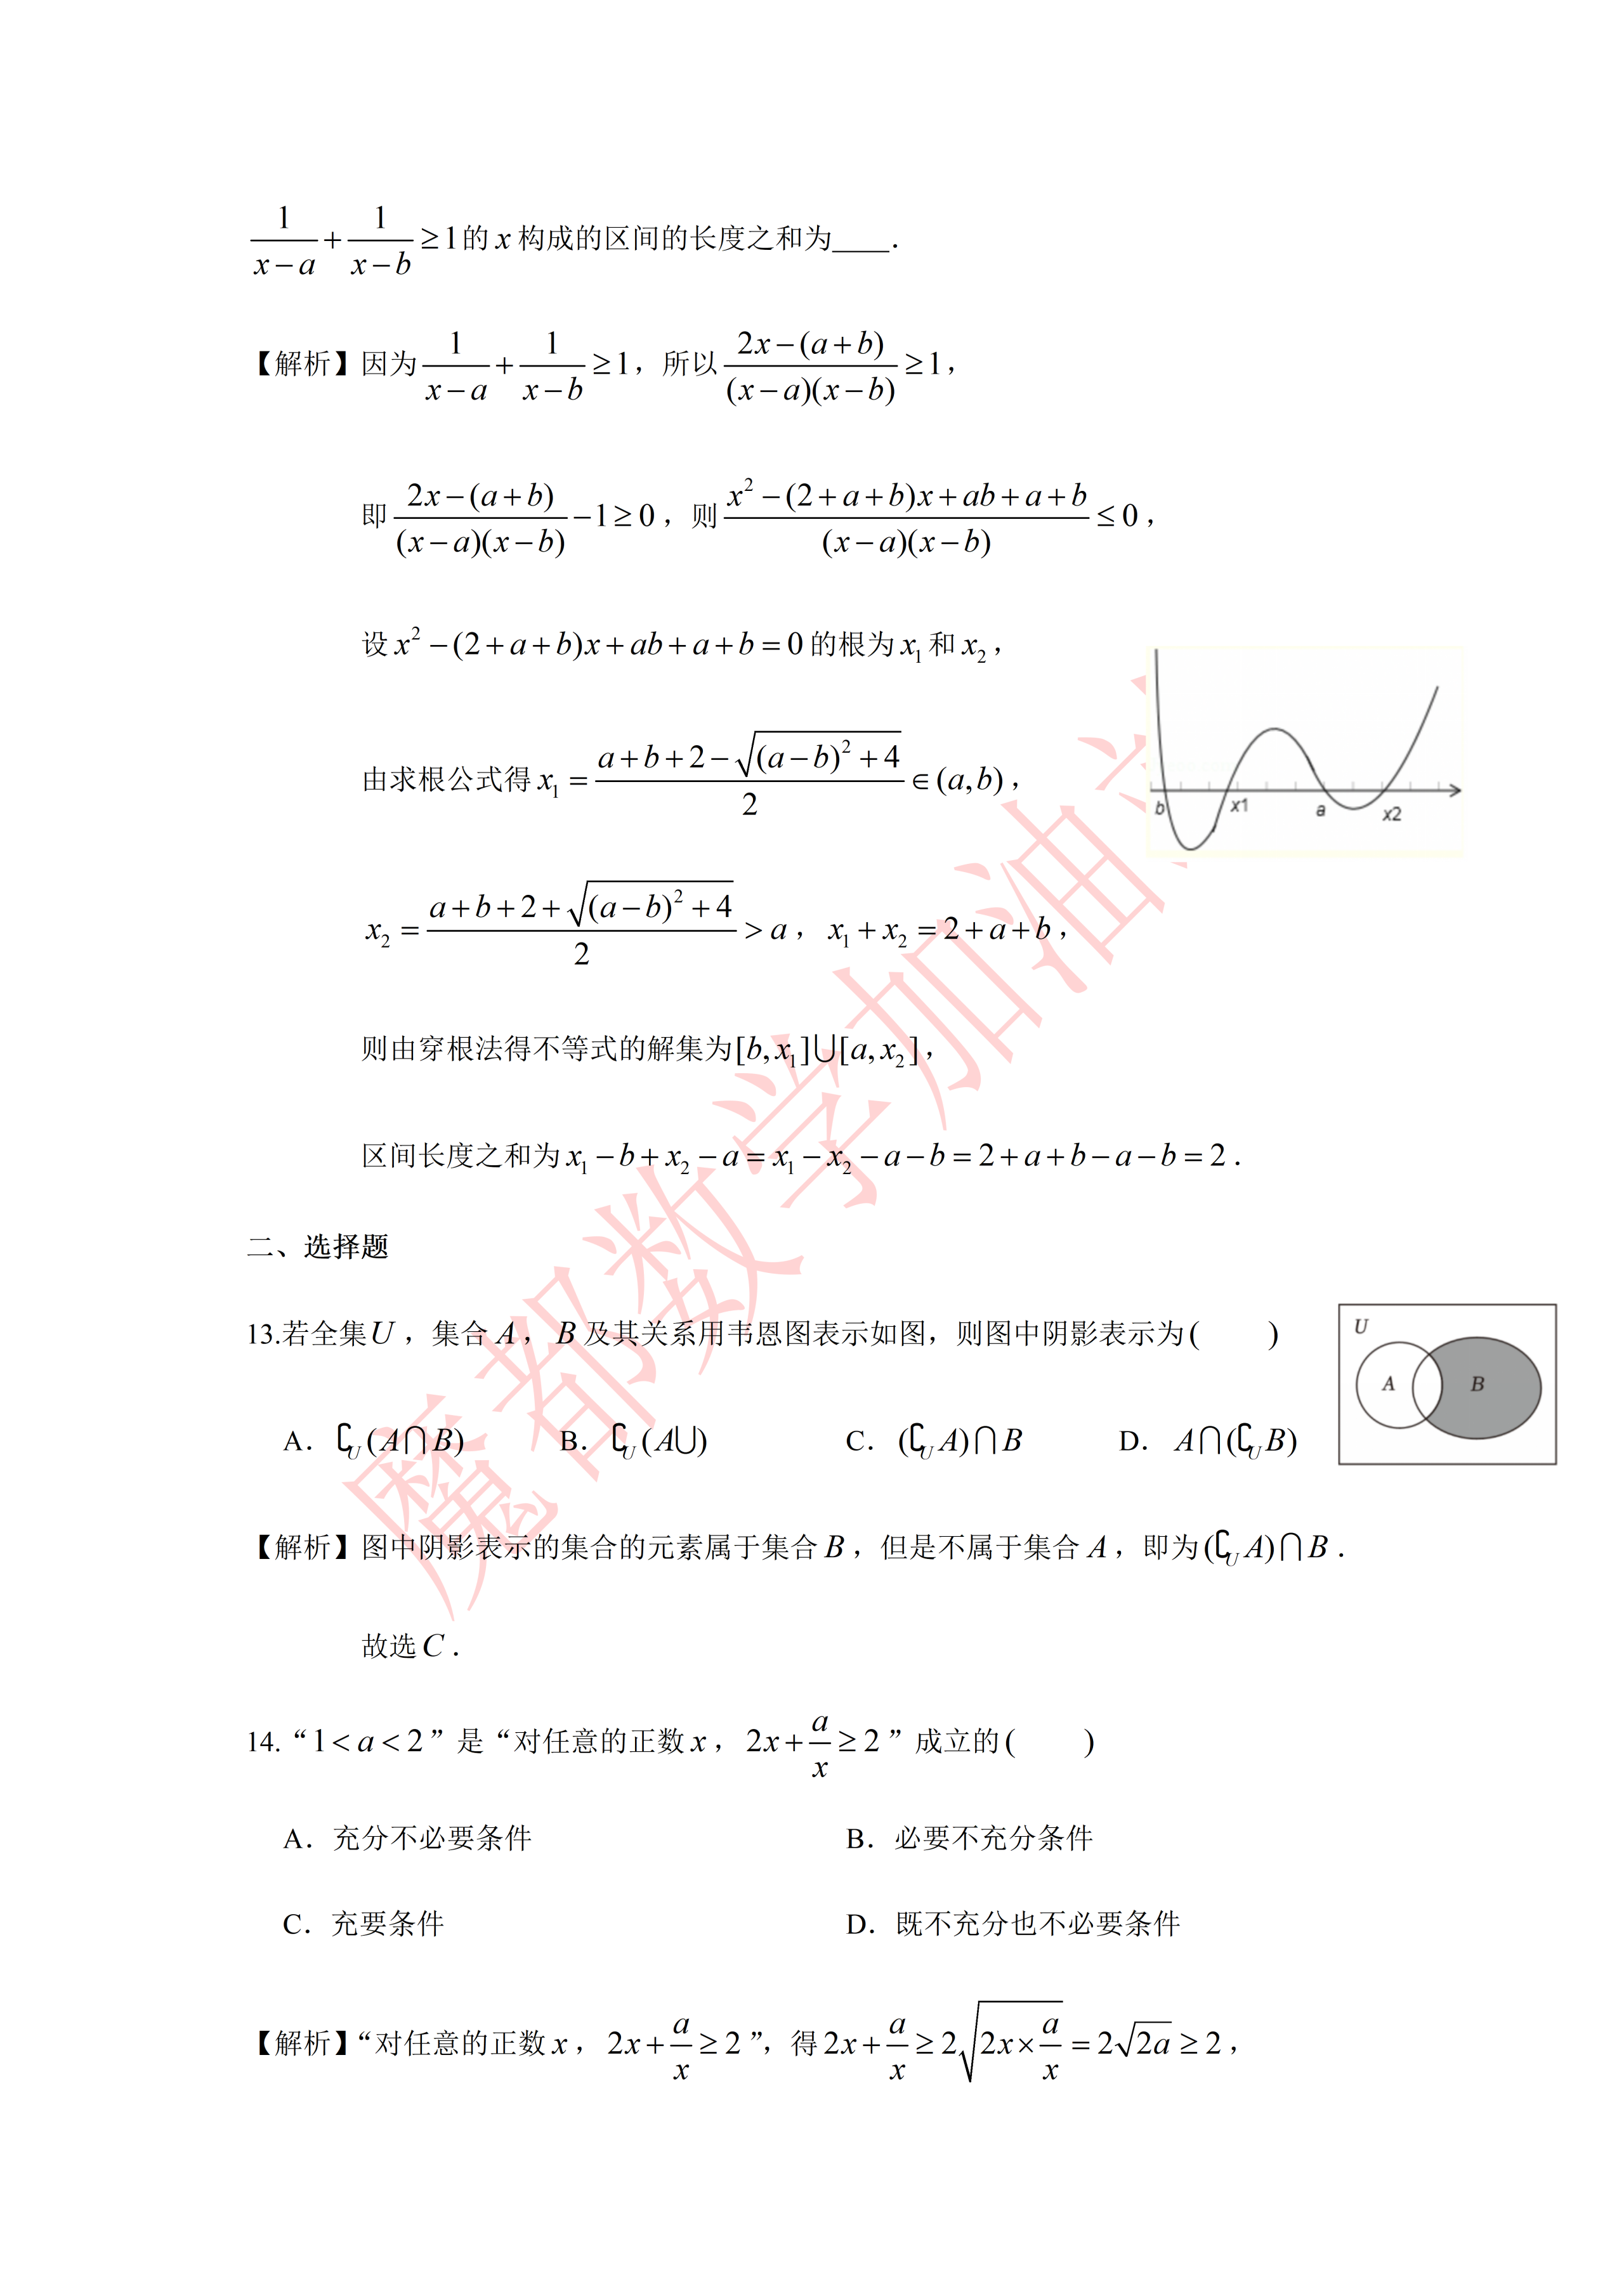
\includegraphics[width=.50\linewidth,trim=1786bp 2255bp 228bp 985bp,clip]{../原图/高一51_华师大二附中_国庆作业3/04.png}
\end{center}
\step{由求根公式得 $x_1=\dfrac{a+b+2-\sqrt{(a-b)^2+4}}{2}\in(a,b)$，}
\step{$x_2=\dfrac{a+b+2+\sqrt{(a-b)^2+4}}{2}>a$，$x_1+x_2=2+a+b$，}
\step{则由穿根法得不等式的解集为 $[b,x_1]\cup[a,x_2]$，}
% 原卷如此，照录未改（此处原卷作 $x_1-x_2$，按上一行 $x_1+x_2=2+a+b$ 当为 $x_1+x_2$）
\step{区间长度之和为 $x_1-b+x_2-a=x_1-x_2-a-b=2+a+b-a-b=2$.}
\solend

\fi

\end{enumerate}

\bigsec{二、选择题}

\begin{enumerate}
\setcounter{enumi}{12}

% 本题是“题干 + 图 + 选项”约 5.5cm 的一整块，图夹在题干与选项之间时 \keepwithprev 挡不住断点，
% 故按 高一30 第 13 题的成例在题前先量一次页高（守卫放在 \item 之前）。
\needvspace{6cm}
\item 若全集 $U$，集合 $A$、$B$ 及其关系用韦恩图表示如图，则图中阴影表示为\mbox{（\quad）}

\begin{center}
% 原卷该图印在题干与选项右侧（原图第 04 页），本稿移作居中排，直接裁取原图，不另存图片文件。
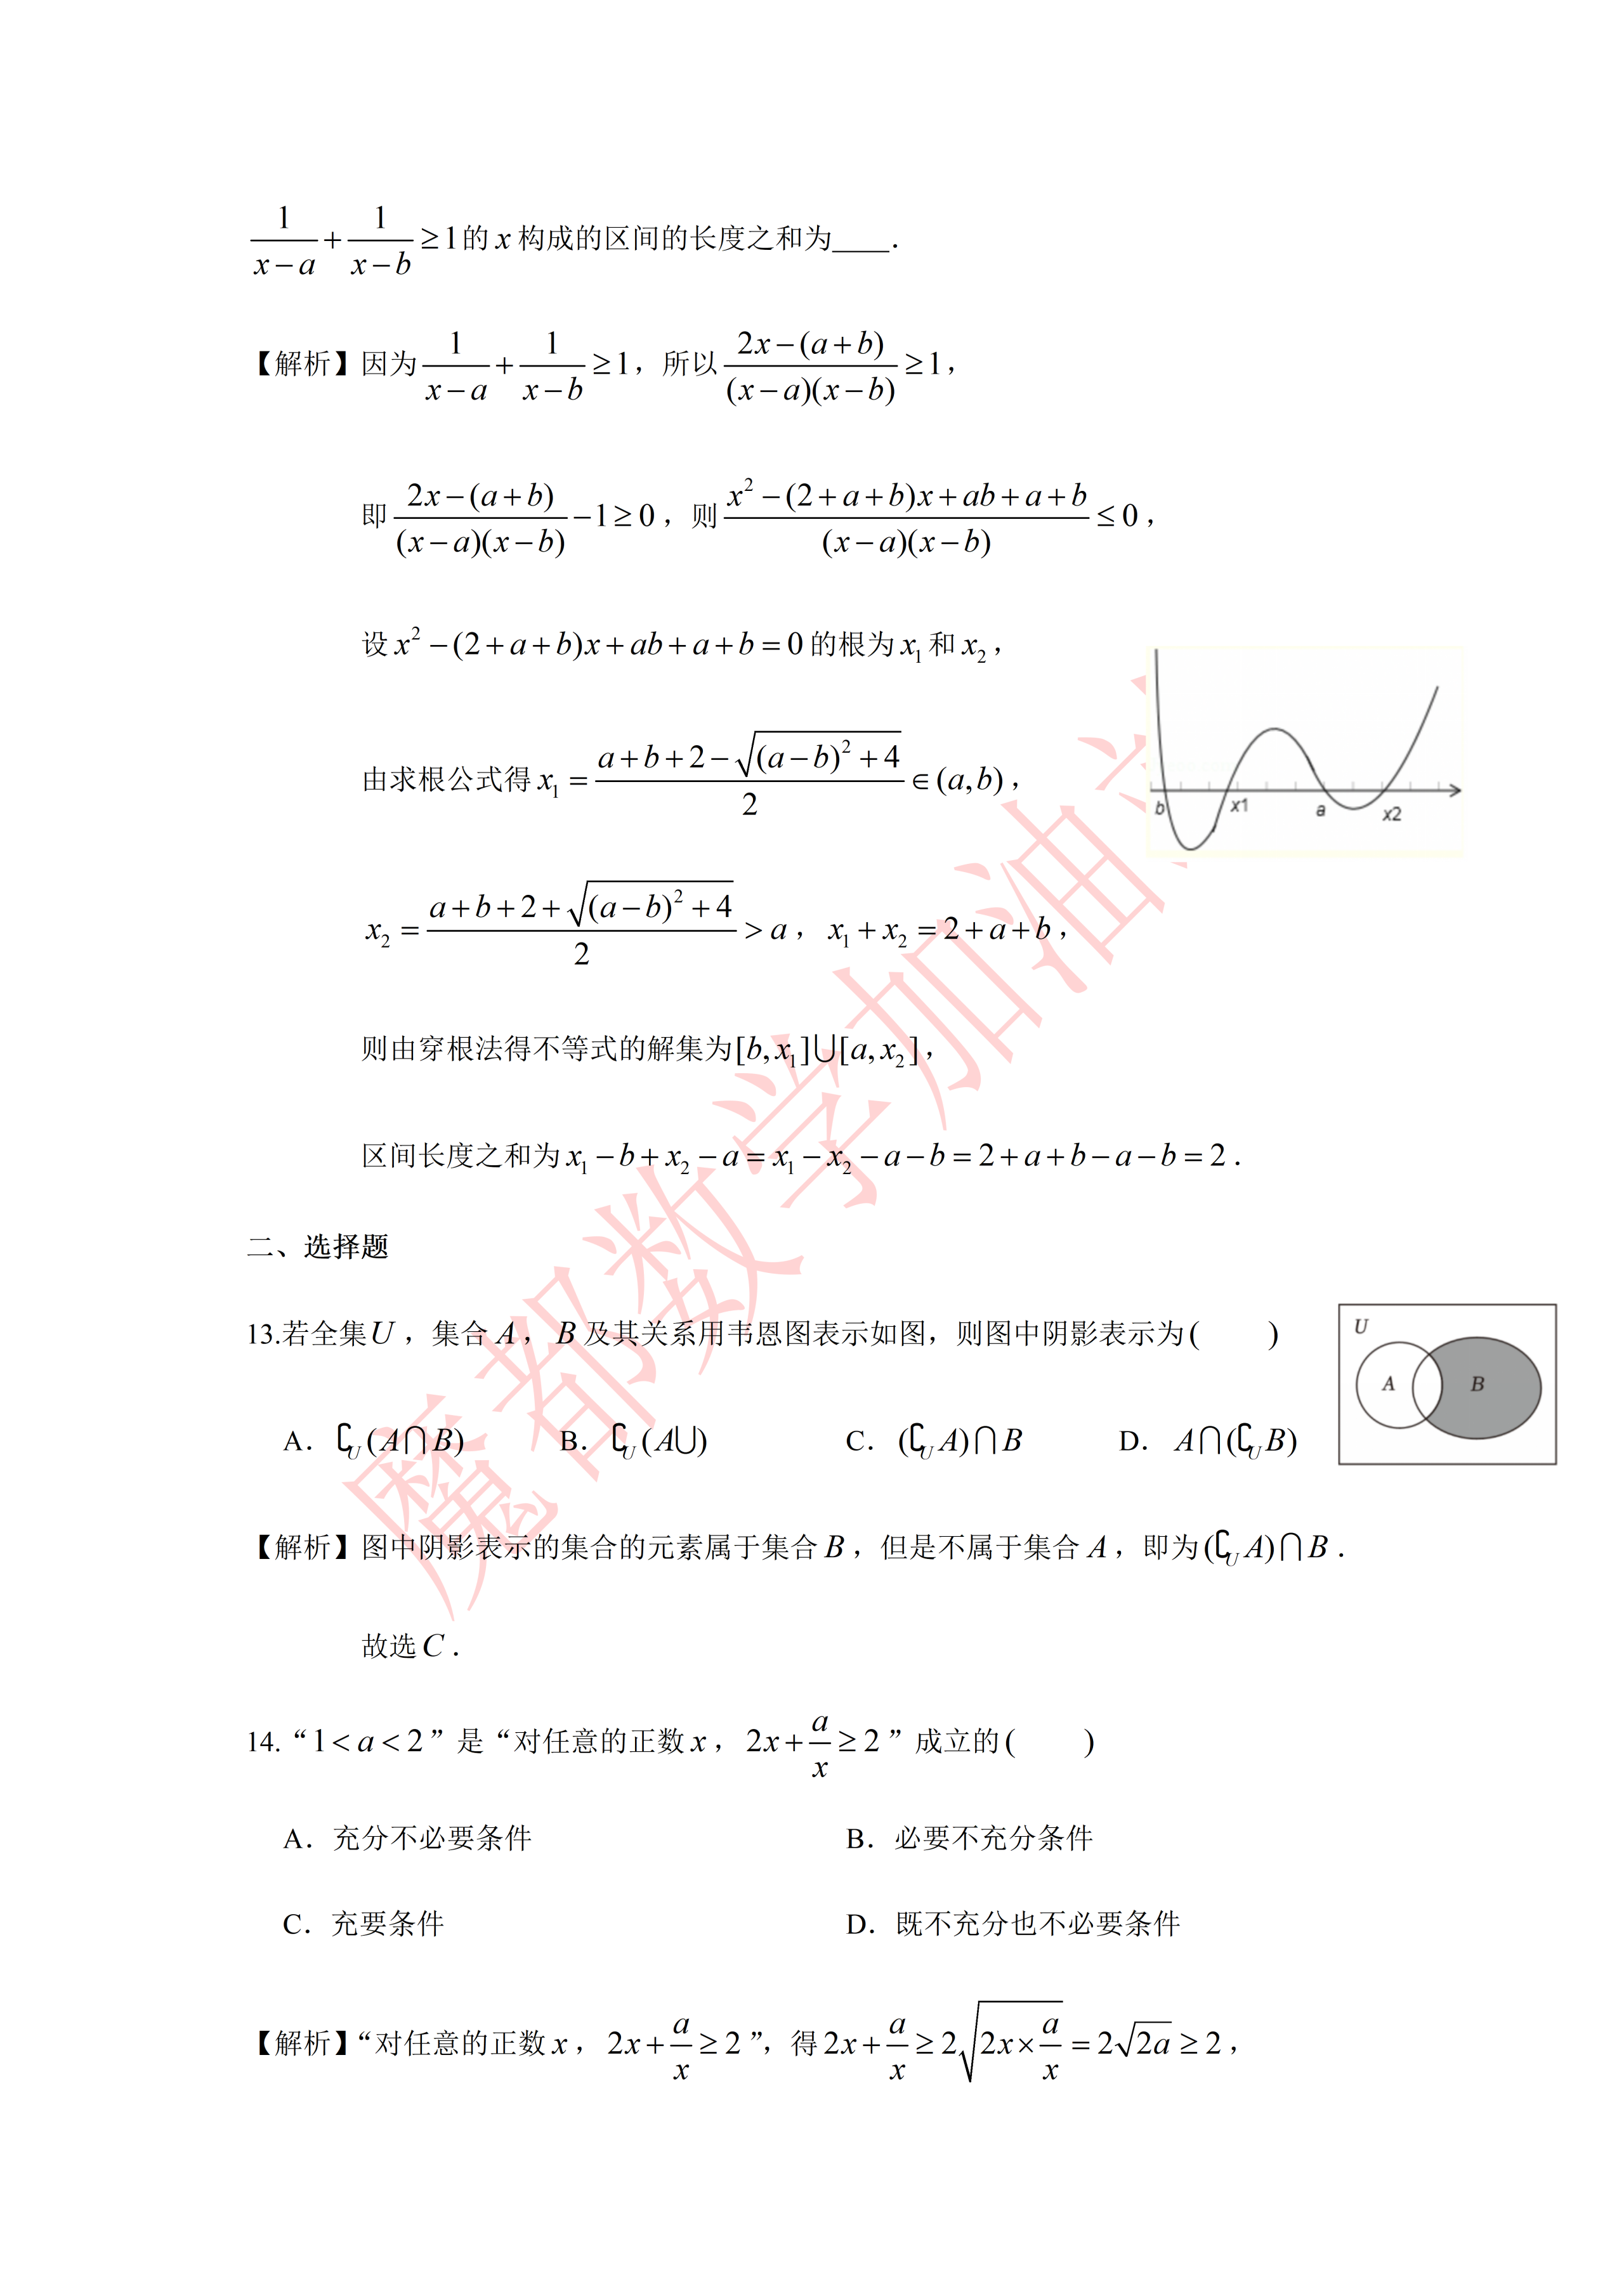
\includegraphics[width=.30\linewidth,trim=2105bp 1308bp 105bp 2050bp,clip]{../原图/高一51_华师大二附中_国庆作业3/04.png}
\end{center}

\keepwithprev
A. $\complement_U(A\cap B)$\qquad B. $\complement_U(A\cup B)$

C. $(\complement_U A)\cap B$\qquad D. $A\cap(\complement_U B)$

\ifanswer
\solbegin
\step{图中阴影表示的集合的元素属于集合 $B$，但是不属于集合 $A$，即为 $(\complement_U A)\cap B$.}
\step{故选 $C$.}
\solend

\fi

\item “$1<a<2$”是“对任意的正数 $x$，$2x+\dfrac ax\geqslant2$”成立的\mbox{（\quad）}

\keepwithprev
A. 充分不必要条件\qquad B. 必要不充分条件

C. 充要条件\qquad\qquad D. 既不充分也不必要条件

\ifanswer
\solbegin
\step{“对任意的正数 $x$，$2x+\dfrac ax\geqslant2$”，得 $2x+\dfrac ax\geqslant2\sqrt{2x\times\dfrac ax}=2\sqrt{2a}\geqslant2$，}
\step{所以 $\sqrt{2a}\geqslant1$，解得 $a\geqslant\dfrac12$，}
\step{若“$1<a<2$”得 $2x+\dfrac ax\geqslant2\sqrt{2x\times\dfrac ax}=2\sqrt{2a}>2\sqrt2>2$，}
\step{所以“$1<a<2$”$\Rightarrow$“对任意的正数 $x$，$2x+\dfrac ax\geqslant2$”，}
\step{所以“$1<a<2$”是“对任意的正数 $x$，$2x+\dfrac ax\geqslant2$”成立的充分不必要条件，}
\step{故选 $A$.}
\solend

\fi

\item 已知函数 $f(x)=2x-3$，$x\in(0,2)$，实数 $a$、$b$ 满足 $f(a)+f(b-1)=0$，则以下成立的有\mbox{（\quad）}

\keepwithprev
A. $a(b-1)$ 的最大值为 $\dfrac94$\qquad\qquad B. $b-\dfrac1a$ 的最大值为 $2$

C. $\dfrac1a+\dfrac1{4b}$ 的最小值为 $\dfrac9{16}$\qquad D. $-1<b-a<3$

\ifanswer
\solbegin
\step{因为函数 $f(x)=2x-3$，$x\in(0,2)$，实数 $a$、$b$ 满足 $f(a)+f(b-1)=0$，}
\step{所以 $2a-3+2(b-1)-3=0$，得 $a+b=4$，$a\in(0,2)$，$b\in(1,3)$，}
\step{所以 $a(b-1)=a(3-a)=-\left(a-\dfrac32\right)^2+\dfrac94$，$a\in(0,2)$，}
\step{所以 $0<a(b-1)\leqslant\dfrac94$，故选项 $A$ 正确；}
\step{$b-\dfrac1a=4-a-\dfrac1a=4-\left(a+\dfrac1a\right)\leqslant4-2=2$，}
\step{当且仅当 $a=1$，$b=3$ 时取等号，又 $b\in(1,3)$，故 $b-\dfrac1a<2$，故 $B$ 错误；}
\step{$\dfrac1a+\dfrac1{4b}=\dfrac14\left(\dfrac1a+\dfrac1{4b}\right)(a+b)=\dfrac14\left(1+\dfrac14+\dfrac ba+\dfrac a{4b}\right)=\dfrac5{16}+\dfrac14\left(\dfrac ba+\dfrac a{4b}\right)$}
\step{$\geqslant\dfrac5{16}+\dfrac14\cdot2\sqrt{\dfrac ba\cdot\dfrac a{4b}}=\dfrac9{16}$，当且仅当 $\dfrac ba=\dfrac a{4b}$，即 $a=2b=\dfrac83$ 时取等号，}
% 原卷如此，照录未改（“又 $a\in(0,2)$，”与下式之间原卷正文夹印“水印”二字）
\step{又 $a\in(0,2)$，水印 $\dfrac1a+\dfrac1{4b}<\dfrac9{16}$，故 $C$ 错误；}
\step{因为 $a\in(0,2)$，$b\in(1,3)$，所以 $-a\in(-2,0)$，所以 $b-a\in(-1,3)$，}
\step{故 $D$ 正确；}
\step{故选 $AD$.}
\solend

\fi

% 本题解析含图（“函数 f(x) 的图像如下”），图夹在解析行间，页末放不下会被拆开，
% 故在题前先量一次页高；上界取“题干 + 选项 + 图 + 首行解析”一块的高度。
\needvspace{6cm}
\item 设 $M_I$ 表示函数 $f(x)=|x^2-4x+2|$ 在闭区间 $I$ 上的最大值. 若正实数 $a$ 满足
$M_{[0,a]}\geqslant2M_{[a,2a]}$，则正实数 $a$ 的取值范围是\mbox{（\quad）}

\keepwithprev
A. $\left[2-\sqrt3,\dfrac12\right]$\qquad B. $[2-\sqrt3,1]$

C. $[2,2+\sqrt3]$\qquad\qquad D. $[2+\sqrt3,4]$

\ifanswer
\solbegin
\step{函数 $f(x)$ 的图像如下：}
\begin{center}
% 原卷该图印在解析行间（原图第 06 页），本稿直接裁取原图，不另存图片文件。
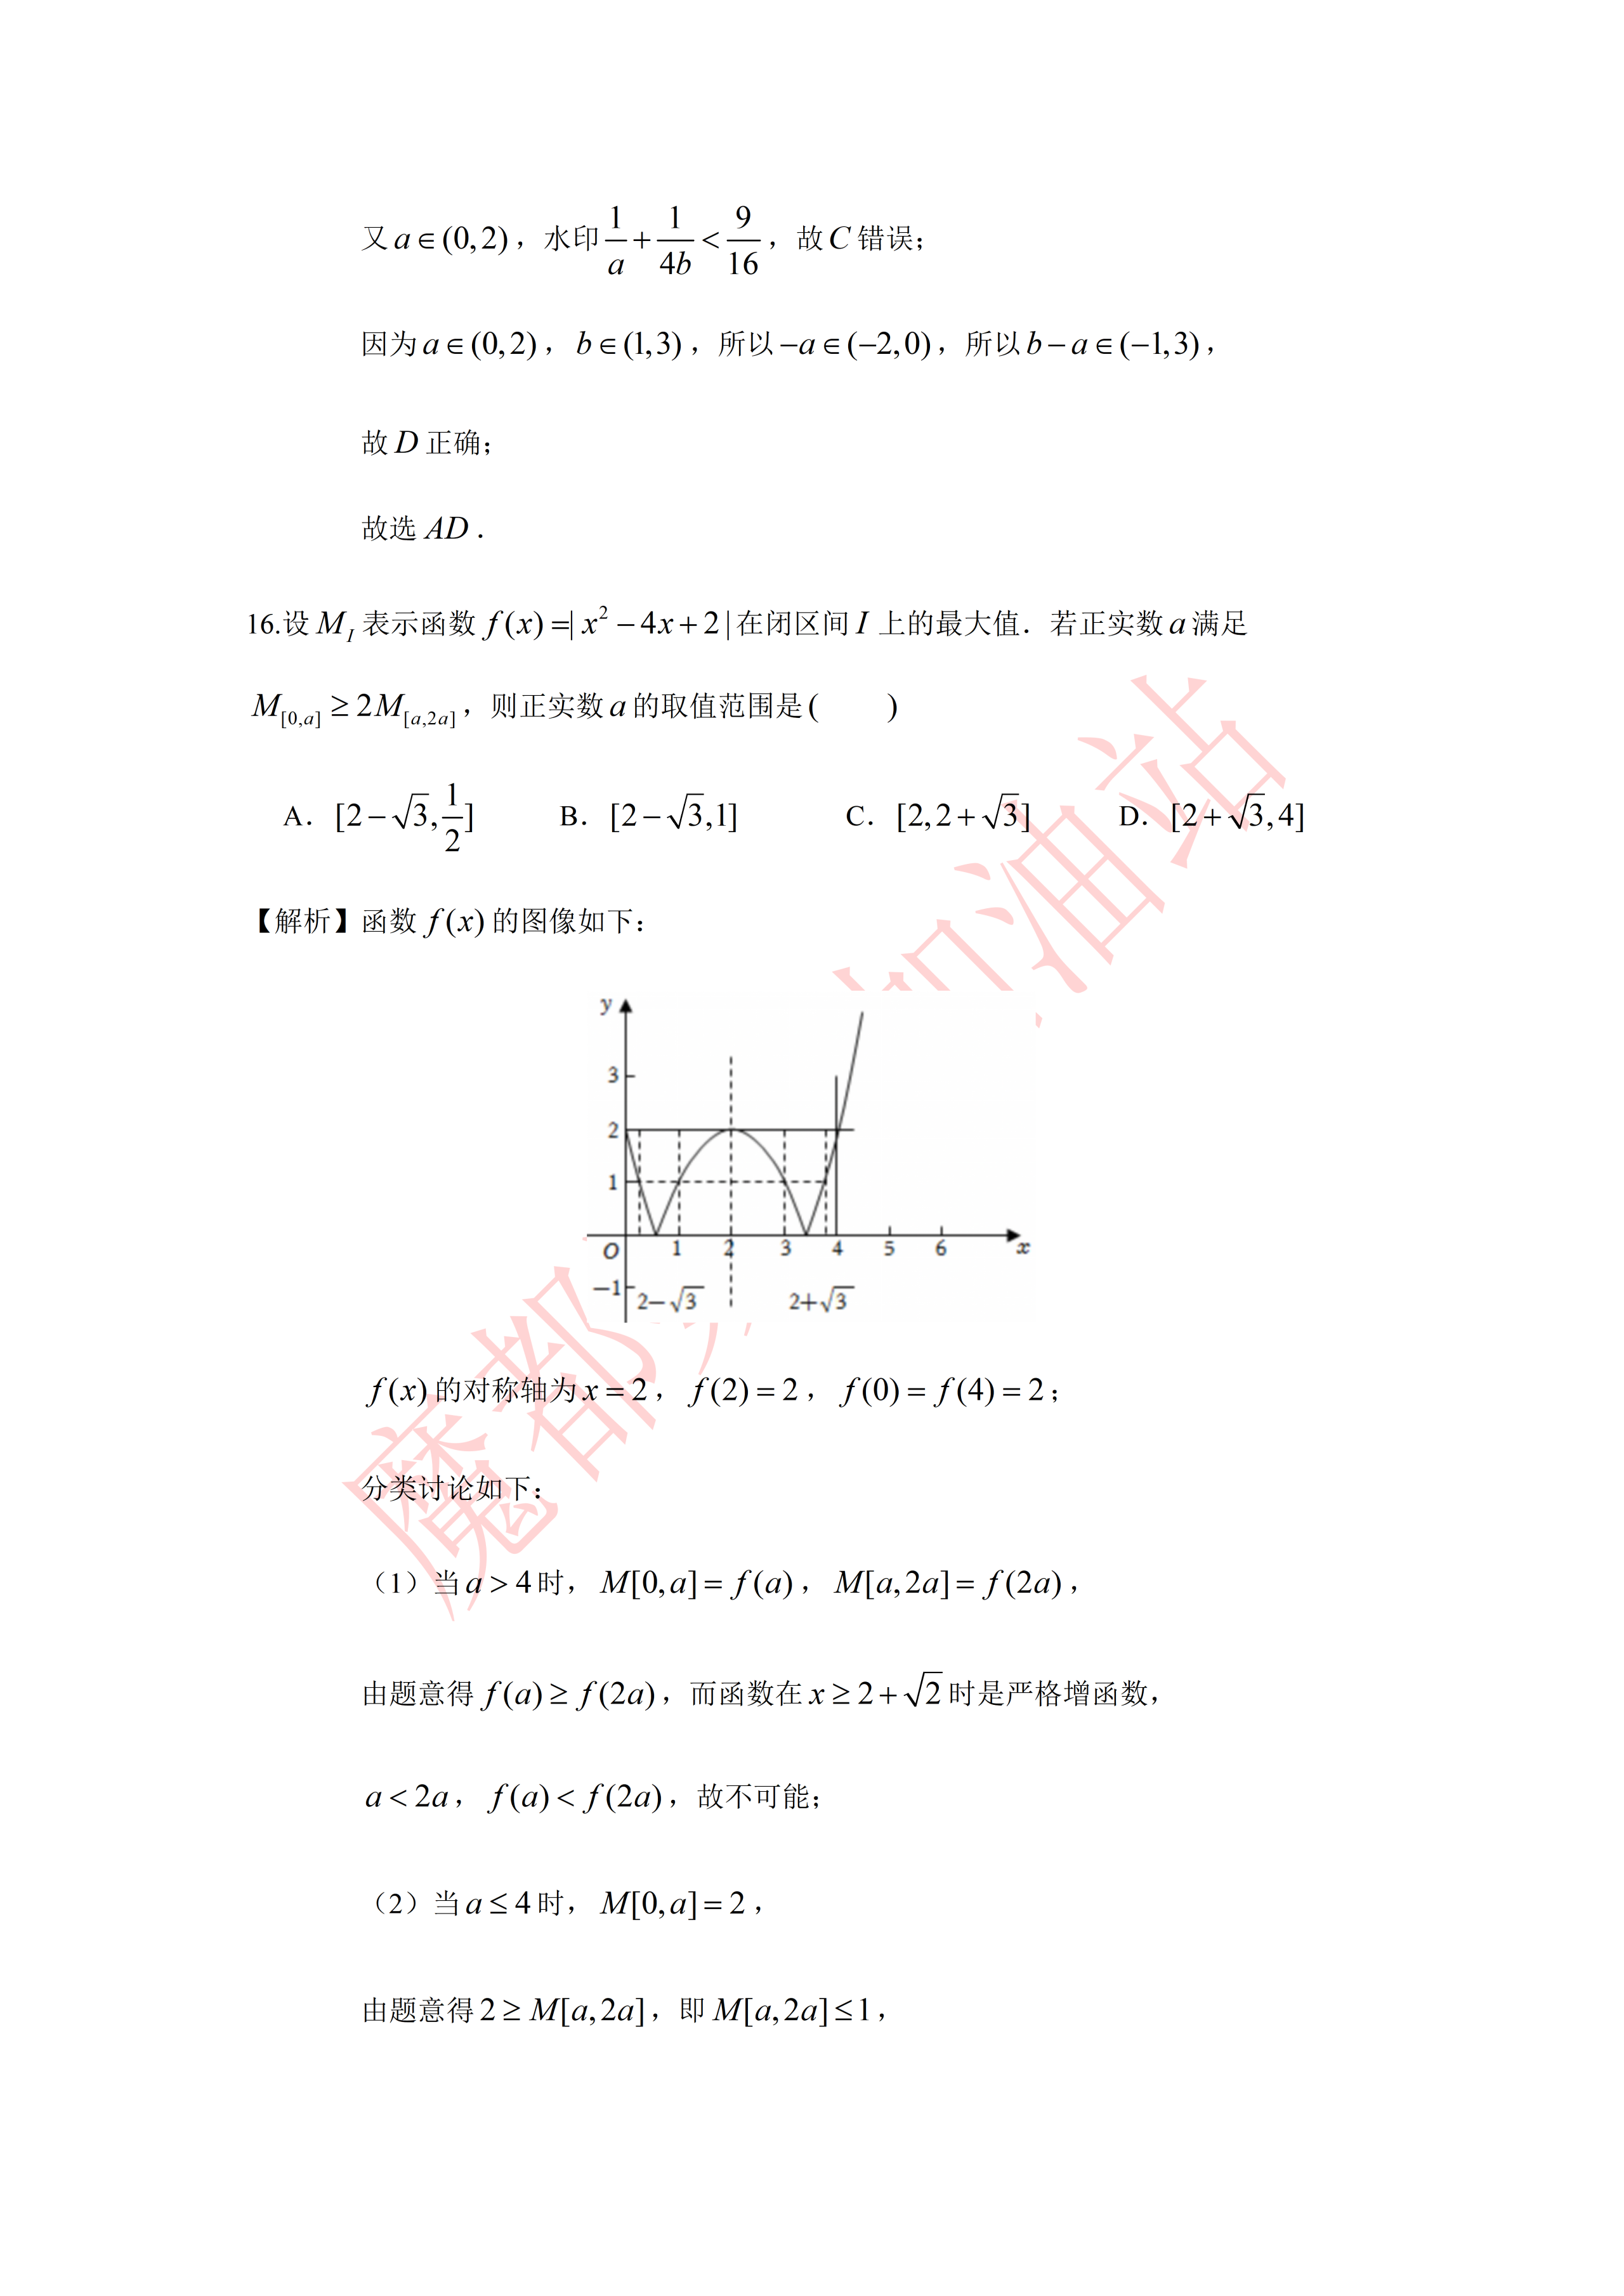
\includegraphics[width=.55\linewidth,trim=895bp 1535bp 915bp 1525bp,clip]{../原图/高一51_华师大二附中_国庆作业3/06.png}
\end{center}
\step{$f(x)$ 的对称轴为 $x=2$，$f(2)=2$，$f(0)=f(4)=2$；}
\step{分类讨论如下：}
\stepm{(1)}{当 $a>4$ 时，$M_{[0,a]}=f(a)$，$M_{[a,2a]}=f(2a)$，}
\step{由题意得 $f(a)\geqslant f(2a)$，而函数在 $x\geqslant2+\sqrt2$ 时是严格增函数，}
\step{$a<2a$，$f(a)<f(2a)$，故不可能；}
\stepm{(2)}{当 $a\leqslant4$ 时，$M_{[0,a]}=2$，}
\step{由题意得 $2\geqslant M_{[a,2a]}$，即 $M_{[a,2a]}\leqslant1$，}
\step{令 $f(x)=1$，解得 $x_1=2-\sqrt3$，$x_2=1$，$x_3=2+\sqrt3$，$x_4=3$，}
\step{则有 $a\geqslant2-\sqrt3$ 并且 $2a\leqslant1$，解得 $2-\sqrt3\leqslant a\leqslant\dfrac12$；}
\step{或者 $a\geqslant3$ 并且 $2a\leqslant2+\sqrt3$，无解；}
\step{故选 $A$.}
\solend

\fi

\end{enumerate}

\bigsec{三、解答题}

\begin{enumerate}
\setcounter{enumi}{16}

\item 已知 $M=\{x\mid2\leqslant x\leqslant5\}$，$N=\{x\mid a-1\leqslant x\leqslant2a+1\}$.
\begin{enumerate}[label=(\arabic*)]
\item 若 $M\subseteq N$，求实数 $a$ 的取值范围；
\item 若 $M\supseteq N$，求实数 $a$ 的取值范围.
\end{enumerate}

\ifanswer
\ans{（1）$[2,3]$；（2）$(-\infty,-2)$}
\fi

\ansspace[6]

\item 设集合 $A=\{x\mid|x+1|\leqslant3\}$，$B=\{x\mid0<x<3m\}$.
\begin{enumerate}[label=(\arabic*)]
\item 若 $A\cup B=A$，求实数 $m$ 的取值范围；
\item 设 $P=(\complement_R A)\cap B$，若 $\exists x\in\Z$ 且 $x\in P$，求实数 $m$ 的取值范围.
\end{enumerate}

\ifanswer
\solbegin
\stepm{(1)}{$A=\{x\mid|x+1|\leqslant3\}=\{x\mid-4\leqslant x\leqslant2\}$，且 $A\cup B=A$，所以 $B\subseteq A$.}
\step{若 $B=\varnothing$，此时 $0\geqslant3m$，解得 $m\leqslant0$；}
\step{若 $B\neq\varnothing$，此时 $0<3m$，且 $3m\leqslant2$，解得 $0<m\leqslant\dfrac23$；}
\step{则实数 $m$ 的取值范围是 $\left(-\infty,\dfrac23\right]$.}
\stepm{(2)}{因为 $\exists x\in\Z$ 且 $x\in P$，所以集合 $P$ 中至少存在一个整数.}
\step{$\complement_R A=\{x\mid x<-4\text{ 或 }x>2\}$，$B=\{x\mid0<x<3m\}$，}
\step{要使 $P=(\complement_R A)\cap B$ 中至少存在一个整数，则 $\begin{cases}3m>0\\3m>3\end{cases}$，解得 $m>1$，}
\step{则实数 $m$ 的取值范围是 $(1,+\infty)$.}
\solend

\fi

\ansspace[7]

\item 已知函数 $f(x)=x^2+(1-a)x-a(a\in\R)$.
\begin{enumerate}[label=(\arabic*)]
\item 解关于 $x$ 的不等式 $f(x)<0$；
\item 若 $\forall a\in[-1,1]$，$f(x)\geqslant0$ 恒成立，求实数 $x$ 的取值范围.
\end{enumerate}

\ifanswer
\solbegin
\stepm{(1)}{不等式 $x^2+(1-a)x-a<0$ 等价于 $(x-a)(x+1)<0$，}
\step{当 $a<-1$ 时，不等式的解集为 $(a,-1)$；}
\step{当 $a=-1$ 时，不等式的解集为 $\varnothing$；}
\step{当 $a>-1$ 时，不等式的解集为 $(-1,a)$.}
\stepm{(2)}{$x^2+(1-a)x-a=-a(x+1)+x^2+x$，}
\step{设 $g(a)=-a(x+1)+x^2+x$，$a\in[-1,1]$，}
\step{要使 $g(a)\geqslant0$ 在 $a\in[-1,1]$ 上恒成立，}
\step{只需 $\begin{cases}g(-1)\geqslant0\\g(1)\geqslant0\end{cases}$，即 $\begin{cases}x^2+2x+1\geqslant0\\x^2-1\geqslant0\end{cases}$，解得 $x\geqslant1$ 或 $x\leqslant-1$，}
\step{所以 $x$ 的取值范围为 $\{x\mid x\leqslant-1\text{ 或 }x\geqslant1\}$.}
\solend

\fi

\ansspace[7]

\item 若实数 $x$、$y$、$m$ 满足 $|x-m|>|y-m|$，则称 $x$ 比 $y$ 远离 $m$.
\begin{enumerate}[label=(\arabic*)]
\item 若 $2$ 比 $3x-4$ 远离 $1$，求 $x$ 的取值范围；
\item 设 $y=\dfrac{x+2}{x+1}$，其中 $x\in(0,\sqrt2)\cup(\sqrt2,+\infty)$，判断：$x$ 与 $y$ 哪一个更远离 $\sqrt2$？并说明理由.
\item 若 $x+y=2$，试问：$y$ 与 $x^2+y^2$ 哪一个更远离 $\dfrac12$？并说明理由.
\end{enumerate}

\ifanswer
\solbegin
\stepm{(1)}{由题意得 $|2-1|>|3x-4-1|$，所以 $|3x-5|<1$，解得 $\dfrac43<x<2$，}
\step{故 $x$ 的取值范围为 $\left(\dfrac43,2\right)$；}
\stepm{(2)}{$x$ 比 $y$ 更远离 $\sqrt2$，}
\step{理由如下：要证 $x$ 比 $y$ 更远离 $\sqrt2$，只要证 $|x-\sqrt2|>\left|\dfrac{x+2}{x+1}-\sqrt2\right|$，}
\step{即证 $|x-\sqrt2|>\left|\dfrac{(1-\sqrt2)(x-\sqrt2)}{x+1}\right|$，}
\step{因为 $x\in(0,\sqrt2)\cup(\sqrt2,+\infty)$，所以 $|x-\sqrt2|>0$，}
\step{所以只要证 $1>\dfrac{\sqrt2-1}{|x+1|}$，即证 $|x+1|>\sqrt2-1$，}
\step{因为 $x\in(0,\sqrt2)\cup(\sqrt2,+\infty)$，所以 $x+1\in(1,\sqrt2+1)\cup(\sqrt2+1,+\infty)$，}
\step{所以 $|x+1|>1>\sqrt2-1$，所以 $x$ 比 $y$ 更远离 $\sqrt2$；}
\stepm{(3)}{因为 $x^2+y^2\geqslant\dfrac{(x+y)^2}{2}=2$，当且仅当 $x=y=1$ 时等号成立，}
\step{所以 $\left|x^2+y^2-\dfrac12\right|=x^2+y^2-\dfrac12$，}
\step{从而 $\left|y-\dfrac12\right|-\left|x^2+y^2-\dfrac12\right|=\left|y-\dfrac12\right|-\left(x^2+y^2-\dfrac12\right)$，}
\step{①$y\geqslant\dfrac12$，$\left|y-\dfrac12\right|-\left|x^2+y^2-\dfrac12\right|=y-\dfrac12-\left(x^2+y^2-\dfrac12\right)=y-x^2-y^2$}
\step{$=y-(2-y)^2-y^2=-2y^2+5y-4=-2\left(y-\dfrac54\right)^2-\dfrac78<0$，}
\step{即 $\left|y-\dfrac12\right|<\left|x^2+y^2-\dfrac12\right|$；}
\step{②$y<\dfrac12$，}
\step{$\left|y-\dfrac12\right|-\left|x^2+y^2-\dfrac12\right|=\left(\dfrac12-y\right)-\left(x^2+y^2-\dfrac12\right)=-y-x^2-y^2+1$}
\step{$=-y-(2-y)^2-y^2+1=-2y^2+3y-3=-2\left(y-\dfrac34\right)^2-\dfrac{15}8<0$，}
\step{即 $\left|y-\dfrac12\right|<\left|x^2+y^2-\dfrac12\right|$；}
\step{综上，$\left|y-\dfrac12\right|<\left|x^2+y^2-\dfrac12\right|$，即 $x^2+y^2$ 比 $y$ 更远离 $\dfrac12$.}
\solend

\fi

\ansspace[9]

\item 对于非空有限整数集 $X$，$m\in\N^*$，定义 $X^m=\{x^m\mid x\in X\}$，对 $n\in\Z$，
$Y\oplus n=\{x+n\mid x\in Y\}$ 现有两个非空有限整数集 $A$、$B$，已知 $A\oplus1\subseteq B$ 且
$B^2\oplus(-4)\subseteq A$.
\begin{enumerate}[label=(\arabic*)]
\item 当 $A=\{-3,0\}$ 时求集合 $B$；
\item 证明：$A\subseteq\{-3,-2,0,1\}$；
\item 当 $A\oplus1=B$ 且 $B^2\oplus(-4)=A$ 时，任取 $a\in A$，$b\in B$ 构造函数
$f(x)=(x-a)(x-b)$ 问：当 $a$、$b$ 取何值时，$f(x)$ 的最小值最小？
\end{enumerate}

\ifanswer
\solbegin
\stepm{(1)}{因为 $A=\{-3,0\}$，$B^2\oplus(-4)\subseteq A$，}
\step{所以 $B^2\oplus(-4)$ 可能为 $\varnothing$、$\{-3\}$、$\{0\}$、$\{-3,0\}$，}
\step{当 $B^2\oplus(-4)=\varnothing$ 时 $B^2=\varnothing$，不满足非空，不合题意；}
\step{当 $B^2\oplus(-4)=\{-3\}$ 时 $B^2=\{1\}$，所以 $B=\{1,-1\}$、$\{1\}$、$\{-1\}$，}
\step{当 $B^2\oplus(-4)=\{0\}$ 时 $B^2=\{4\}$，所以 $B=\{2,-2\}$、$\{2\}$、$\{-2\}$，}
% 原卷如此，照录未改（此处作 $\{0,-3\}$，上一行同一集合作 $\{-3,0\}$）
\step{当 $B^2\oplus(-4)=\{0,-3\}$ 时 $B^2=\{4,1\}$，}
\step{所以 $B=\{1,2,-1,-2\}$、$\{2,-1,-2\}$、$\{2,1,-2\}$、$\{1,-1,-2\}$、$\{1,-1,2\}$、$\{1,2\}$、$\{-1,2\}$、$\{-1,-2\}$、$\{1,-2\}$，}
\step{又 $A\oplus1=\{-2,1\}\subseteq B$，得 $B$ 为 $\{1,-2\}$、$\{2,1,-2\}$、$\{1,-1,-2\}$、$\{1,2,-1,-2\}$.}
\stepm{(2)}{设 $x\in A$，因为 $A\oplus1\subseteq B$，所以 $x+1\in B$，}
\step{又 $B^2\oplus(-4)\subseteq A$，所以 $(x+1)^2-4\in A$，}
% 原卷如此，照录未改（此处及下文取 $x=2$ 处原卷均作 $(-4+1)^2-4=52-2a>0$）
\step{取 $x=-4$，则 $(-4+1)^2-4=52-2a>0$，$(5+1)^2-4=32\in A$，$\cdots$，}
\step{无限迭代，而 $A$ 为有限集，不合题意，舍去，即 $-4\notin A$；}
\step{取 $x=-3$，则 $(-3+1)^2-4=0\in A$，$(0+1)^2-4=-3\in A$，}
\step{得 $A$ 集合可为 $\{-3,0\}$；}
\step{取 $x=-2$，则 $(-2+1)^2-4=-3\in A$，$(-3+1)^2-4=0\in A$，}
\step{$(0+1)^2-4=-3\in A$，得 $A$ 集合可为 $\{-3,-2,0\}$；}
\step{取 $x=-1$，则 $(-1+1)^2-4=-4\in A$，又 $-4\notin A$，所以 $-1\notin A$，}
\step{取 $x=1$，则 $(1+1)^2-4=0\in A$，$(0+1)^2-4=-3\in A$，}
\step{$(-3+1)^2-4=0\in A$，得 $A$ 集合可为 $\{-3,0,1\}$，}
\step{取 $x=2$，则 $(2+1)^2-4=52-2a>0$，$(5+1)^2-4=32\in A$，$\cdots$，}
\step{无限迭代，而 $A$ 为有限集，不合题意，舍去，即 $2\notin A$，}
\step{同理当 $x<-4$ 或 $x>2$，且 $x\in\Z$ 时不符合 $A$ 为有限集，舍去；}
\step{故由上得 $A$ 集合可为 $\{-3,0\},\{-3,-2,0\},\{-3,0,1\},\{-3,-2,0,1\}$，}
\step{所以 $A\subseteq\{-3,-2,0,1\}$，}
\stepm{(3)}{当 $A\oplus1=B$ 且 $B^2\oplus(-4)=A$ 时，}
\step{设 $x\in B$，则 $x^2-4\in B^2\oplus(-4)=A$，}
% 原卷如此，照录未改（题设 $A=\{-3,0\}$，此处两个判别式取的是 $-2$ 与 $1$，均不属于 $A$）
\step{$x^2-4=-2$ 时 $x=\pm\sqrt2$，不为整数，不合题意；}
\step{$x^2-4=1$ 时 $x=\pm\sqrt5$，不为整数，不合题意；}
\step{所以 $A=\{-3,0\}$，又 $A\oplus1=B$，则 $B=\{-2,1\}$，}
\step{任取 $a\in A$，$b\in B$ 构造函数 $f(x)=(x-a)(x-b)$，}
\step{$f(x)=(x-a)(x-b)=x^2-(a+b)x+ab$}
\step{$=x^2-(a+b)x+\dfrac{(a+b)^2}{4}+ab-\dfrac{(a+b)^2}{4}$}
\step{$=\left[x-\dfrac{(a+b)}2\right]^2-\dfrac{(a-b)^2}{4}\geqslant-\dfrac{(a-b)^2}{4}$，所以 $f(x)_{min}=-\dfrac{(a-b)^2}{4}$，}
\step{又 $a\in A=\{-3,0\}$，$b\in B=\{-2,1\}$，所以 $a-b$ 的取值有 $-1,-4,2$，}
\step{所以 $f(x)_{min}=-\dfrac{(a-b)^2}{4}\geqslant-\dfrac{(-3-1)^2}{4}=-4$，}
\step{即当 $a=-3$，$b=1$ 时 $f(x)_{min}$ 的最小值为 $-4$.}
\solend

\fi

\ansspace*[12]

\end{enumerate}

\end{document}
"
%
% 原始材料：微信公众号“魔都数学加油站”文章，作者破晓，连载“27学年高一51”；
% 原文标题“27学年高一51——2026-2027年上海市华师大二附中高一上国庆作业3”；
% 原文链接：https://mp.weixin.qq.com/s/95SLMEmPUT30s4U7wjr5Og。
% 该页面用 JS 渲染，未见明确发布日期；页面内时间戳约为 2026-10-05 21:37，本稿以该时刻记可得日期。
% 正文为 12 张 PNG 页：第 01、02、03、05、07、08、11 页 4762×6735，
% 第 04、06、09、10、12 页 2560×3620。按页序逐页读取，12 页全为试卷正文页
% （卷首标题在第 1 页页顶，卷末解答题止于第 12 页），无封面页、目录页或单独的页脚页。
% 卷面标题照原卷印作“2026-2027 年华师大二附中高一上国庆作业 3”（公众号标题中的“上海市”
% 卷面标题行没有，本稿照卷面），年份区间按全稿惯例排 en dash。
%
% 篇幅与题号：原卷自第 3 题起编号（第 1、2 题不在本卷内）。填空题 3—12（10 题）、
% 选择题 13—16（4 题）、解答题 17—21（5 题），共 19 题。本稿沿用原节与原题号，
% 只改排为全稿统一的大节样式（原卷小节标题为“一、填空题”“二、选择题”“三、解答题”）。
% 正文为讲评版：填空题 3—12 与选择题 13—16 只印【解析】（选择题的结论“故选 X”印在解析内），
% 按全稿口径这类题不另提 \ans{}；解答题第 17 题只印【答案】，故只给 \ans{}；
% 第 18—21 题只印【解析】。
%
% 副标题：原卷未印副标题。本稿按“知识模块”口径标作“集合与常用逻辑用语、不等式”：
% 19 题中集合与常用逻辑用语 8 题（3、4、6、10、13、17、18、21），
% 不等式（含函数最值、绝对值不等式）11 题（5、7、8、9、11、12、14、15、16、19、20），
% 两类均远超三分之一，故并标。口径同 高一46_交附闵行_国庆作业3、高一48_华师大二附中_周末作业2。
%
% 与原卷的排版差异：
%   ① 原卷每题下直接印【答案】或【解析】，本稿按全稿惯例将答案与解析置于答案版；
%   ② 原卷未印副标题，本稿按“知识模块”口径补出；
%   ③ 原卷填空横线按全稿惯例排为 \blankline[4.4em]；
%   ④ 原卷 $R$、$N$、$Z$ 均排斜体，本稿按全稿惯例改用花体 $\R$、$\N$、$\Z$（同 高一48）；
%   ⑤ 原卷第 12 题解析配图、第 13 题题干韦恩图都印在正文右侧的浮动位置，第 16 题解析配图
%      印在解析行间；本稿三图一律居中排，均自原图对应页裁切（trim），不另存图片文件；
%   ⑥ 原卷解答题未留作答空白，本稿按全稿惯例加 \ansspace；
%   ⑦ 原卷第 15 题解析第 7、8 两个印刷行是一串连等式的折行，本稿按“一条 \step ＝ 一个印刷行”
%      的口径分成两条 \step。
%
% 原卷笔误/存疑（均照录未改，正文对应处另有 % 注）：
%   ① 第 12 题解析末行作“区间长度之和为 $x_1-b+x_2-a=x_1-x_2-a-b=2+a+b-a-b=2$”，
%      按上一行 $x_1+x_2=2+a+b$，此处应为 $x_1+x_2$；原卷作 $x_1-x_2$。
%   ② 第 15 题解析“又 $a\in(0,2)$，”与 $\dfrac1a+\dfrac1{4b}<\dfrac9{16}$ 之间，
%      原卷正文夹印“水印”二字（系制版遗留字样，非试卷内容）。
%   ③ 第 21 题第 (2) 问解析两处（取 $x=-4$、取 $x=2$）作“$=52-2a>0$”，
%      与题设 $(x+1)^2-4$ 的取值（按 $x=-4$ 应为 $5$）不符，当系原卷算式遗留。
%   ④ 第 21 题第 (1) 问解析先写 $B^2\oplus(-4)$ 可能为 $\{-3,0\}$，后文又作 $\{0,-3\}$，
%      同一集合两种写法。
%   ⑤ 第 21 题第 (3) 问解析：题设 $B^2\oplus(-4)=A$ 且 $A=\{-3,0\}$ 时，由 $x^2-4\in A$
%      应得 $x^2-4=-3$ 或 $0$；原卷讨论的却是 $x^2-4=-2$ 与 $x^2-4=1$（两值均不属于 $A$），
%      与题设不合。
%
% 插图：3 张，均自原图裁切（无 \begin{tikzpicture} 重排）：
%   · 第 13 题题干韦恩图（原图第 04 页，图在题干与选项右侧）
%   · 第 12 题解析配图（原图第 04 页，图在解析右侧）
%   · 第 16 题解析配图（原图第 06 页，图在解析中间）
%
\documentclass[a4paper,11pt]{article}
\usepackage{common}

\begin{document}

\examtitlest[3]{2026--2027 年华师大二附中高一上国庆作业 3}{集合与常用逻辑用语、不等式}

\bigsec{一、填空题}

\begin{enumerate}
\setcounter{enumi}{2}

\item 若 $\{x\mid x<1\text{ 或 }x>4\}\cup\{x\mid m<x<2m+3\}=R$，则实数 $m$ 的取值范围为\blankline[4.4em].

\ifanswer
\solbegin
\step{因为 $\{x\mid x<1\text{ 或 }x>4\}\cup\{x\mid m<x<2m+3\}=R$，}
\step{所以 $\begin{cases}m<1\\2m+3>4\end{cases}$，解得 $\dfrac12<m<1$，所以 $m$ 的取值范围为 $\left(\dfrac12,1\right)$.}
\solend

\fi

\item 若“$x\leqslant5$”是“$x<a$”的必要不充分条件，则 $a$ 的取值范围是\blankline[4.4em].

\ifanswer
\solbegin
\step{若“$x\leqslant5$”是“$x<a$”的必要不充分条件，则 $\{x\mid x<a\}\subset\{x\mid x\leqslant5\}$，}
\step{所以 $a\leqslant5$.}
\solend

\fi

\item 实数 $x$、$y$ 满足 $x^2+2xy+4y^2=1$，则 $x+2y$ 的取值范围是\blankline[4.4em].

\ifanswer
\solbegin
\step{因为 $x^2+2xy+4y^2=(x+2y)^2-2xy=1$，}
\step{所以 $(x+2y)^2-1=x\cdot(2y)\leqslant\left(\dfrac{x+2y}{2}\right)^2$，当且仅当 $x=2y$ 时取等号，}
\step{解得 $-\dfrac{2\sqrt3}{3}\leqslant x+2y\leqslant\dfrac{2\sqrt3}{3}$，故 $x+2y$ 的取值范围是 $\left[-\dfrac{2\sqrt3}{3},\dfrac{2\sqrt3}{3}\right]$.}
\solend

\fi

\item 若命题 $p$：“$\exists x\in\R$，$5x^2-3x+m=0$”为假命题，则实数 $m$ 的取值范围为\blankline[4.4em].

\ifanswer
\solbegin
\step{若命题 $p$：$\exists x\in\R$，$5x^2-3x+m=0$ 为假命题，}
\step{则 $5x^2-3x+m=0$ 没有实数根，故 $\Delta=9-20m<0$，解得 $m>\dfrac9{20}$.}
\solend

\fi

\item 若当 $3\leqslant m\leqslant5$ 时，$mx^2-mx+m-9<0$ 有解，则实数 $x$ 的取值范围是\blankline[4.4em].

\ifanswer
\solbegin
\step{当 $3\leqslant m\leqslant5$ 时，$mx^2-mx+m-9<0$ 有解，}
\step{即 $(x^2-x+1)m-9<0$ 在 $m\in[3,5]$ 上有解，}
\step{因为 $x^2-x+1>0$，所以一次函数 $g(m)=(x^2-x+1)m-9$ 严格增，}
\step{所以只需 $g(3)=3x^2-3x-6<0$ 即可，}
\step{即 $x^2-x-2<0$，$(x-2)(x+1)<0$，解得 $-1<x<2$，}
\step{所以实数 $x$ 的取值范围是 $(-1,2)$.}
\solend

\fi

\item 已知不等式 $\dfrac{x}{x^2+4}\leqslant a$ 对任意的 $x\in[1,3]$ 恒成立，则实数 $a$ 的范围为\blankline[4.4em].

\ifanswer
\solbegin
\step{因为 $x\in[1,3]$，所以 $\dfrac{x}{x^2+4}=\dfrac{1}{x+\dfrac4x}\leqslant\dfrac{1}{2\sqrt{x\times\dfrac4x}}=\dfrac14$，}
\step{当且仅当 $x=\dfrac4x$ 时，即 $x=2$ 时取等号，即 $\dfrac{x}{x^2+4}$ 在 $x\in[1,3]$ 的最大值为 $\dfrac14$，}
\step{又由不等式 $\dfrac{x}{x^2+4}\leqslant a$ 对任意的 $x\in[1,3]$ 恒成立，所以 $a\geqslant\dfrac14$，}
\step{即实数 $a$ 的范围为 $\left[\dfrac14,+\infty\right)$.}
\solend

\fi

\item 甲、乙两人解关于 $x$ 的不等式 $x^2+bx+c<0$，甲写错了 $b$，正确计算后得到的解为 $\{x\mid1<x<2\}$；
乙写错了 $c$，正确计算后得到的解为 $\{x\mid-4<x<1\}$. 那么不等式 $\dfrac{bx+c}{x-2}<0$ 的解为\blankline[4.4em].

\ifanswer
\solbegin
\step{由 $x^2+bx+c<0$ 的解为 $\{x\mid1<x<2\}$，}
\step{则 $1$ 和 $2$ 是方程 $x^2+bx+c=0$ 的两个根，}
\step{甲写错了 $b$，但 $c$ 是正确的，所以 $c=1\times2=2$；}
\step{由 $x^2+bx+c<0$ 的解为 $\{x\mid-4<x<1\}$，}
\step{则 $-4$ 和 $1$ 是方程 $x^2+bx+c=0$ 的两个根，}
\step{乙写错了 $c$，但 $b$ 是正确的，所以 $-b=-4+1=-3$，即 $b=3$.}
\step{由 $\dfrac{bx+c}{x-2}<0$，得 $\dfrac{3x+2}{x-2}<0$，即 $(3x+2)(x-2)<0$，解得 $-\dfrac23<x<2$.}
\step{不等式 $\dfrac{bx+c}{x-2}<0$ 的解为 $\left\{x\mid-\dfrac23<x<2\right\}$.}
\solend

\fi

\item 已知 $\dfrac{1}{x-2}\geqslant1$ 是 $|x-a|<2$ 的充分非必要条件，则实数 $a$ 的取值范围是\blankline[4.4em].

\ifanswer
\solbegin
\step{由 $\dfrac{1}{x-2}\geqslant1$ 得 $\dfrac{3-x}{x-2}\geqslant0$，解得 $2<x\leqslant3$，由 $|x-a|<2$ 得 $a-2<x<a+2$，}
\step{因为 $\dfrac{1}{x-2}\geqslant1$ 是 $|x-a|<2$ 的充分非必要条件，}
\step{所以 $\{x\mid2<x\leqslant3\}\subset\{x\mid a-2<x<a+2\}$，所以 $\begin{cases}a-2\leqslant2\\a+2>3\end{cases}$，解得 $1<a\leqslant4$，}
\step{即实数 $a$ 的取值范围是 $(1,4]$.}
\solend

\fi

\item 设 $a>0$，$b>0$，若不等式 $a(a+1)^2+b(b+1)^2\geqslant\lambda ab$ 恒成立，则实数 $\lambda$ 的最大值为\blankline[4.4em].

\ifanswer
\solbegin
\step{$a(a+1)^2+b(b+1)^2\geqslant\lambda ab\Leftrightarrow\lambda\leqslant\dfrac{a(a+1)^2+b(b+1)^2}{ab}=\dfrac{(a+1)^2}{b}+\dfrac{(b+1)^2}{a}$，}
\step{从而原问题转化为求 $\dfrac{(a+1)^2}{b}+\dfrac{(b+1)^2}{a}$ 的最小值.}
\step{因为 $\dfrac{(a+1)^2}{b}+\dfrac{(b+1)^2}{a}=\dfrac{b^2+2b+1}{a}+\dfrac{a^2+2a+1}{b}$}
\step{$=\left(\dfrac{b^2}{a}+\dfrac{a^2}{b}\right)+2\left(\dfrac ba+\dfrac ab\right)+\left(\dfrac1a+\dfrac1b\right)\geqslant2\sqrt{\dfrac{b^2}{a}\cdot\dfrac{a^2}{b}}+2\times2\sqrt{\dfrac ba\cdot\dfrac ab}+2\sqrt{\dfrac1a\cdot\dfrac1b}$}
\step{$=2\sqrt{ab}+4+\dfrac{2}{\sqrt{ab}}\geqslant2\sqrt{2\sqrt{ab}\cdot\dfrac{2}{\sqrt{ab}}}+4=8$，以上均当且仅当 $a=b$ 时取等号，}
\step{所以 $\lambda\leqslant8$，即实数 $\lambda$ 的最大值为 $8$.}
\solend

\fi

\item 定义区间 $(a,d)$、$[a,d)$、$(a,d]$、$[a,d]$ 的长度为 $d-a$（$d>a$），已知 $a>b$，则满足
$\dfrac{1}{x-a}+\dfrac{1}{x-b}\geqslant1$ 的 $x$ 构成的区间的长度之和为\blankline[4.4em].

\ifanswer
\solbegin
\step{因为 $\dfrac{1}{x-a}+\dfrac{1}{x-b}\geqslant1$，所以 $\dfrac{2x-(a+b)}{(x-a)(x-b)}\geqslant1$，}
\step{即 $\dfrac{2x-(a+b)}{(x-a)(x-b)}-1\geqslant0$，则 $\dfrac{x^2-(2+a+b)x+ab+a+b}{(x-a)(x-b)}\leqslant0$，}
\step{设 $x^2-(2+a+b)x+ab+a+b=0$ 的根为 $x_1$ 和 $x_2$，}
\begin{center}
% 原卷该图印在解析右侧（原图第 04 页），本稿移作居中排，直接裁取原图，不另存图片文件。
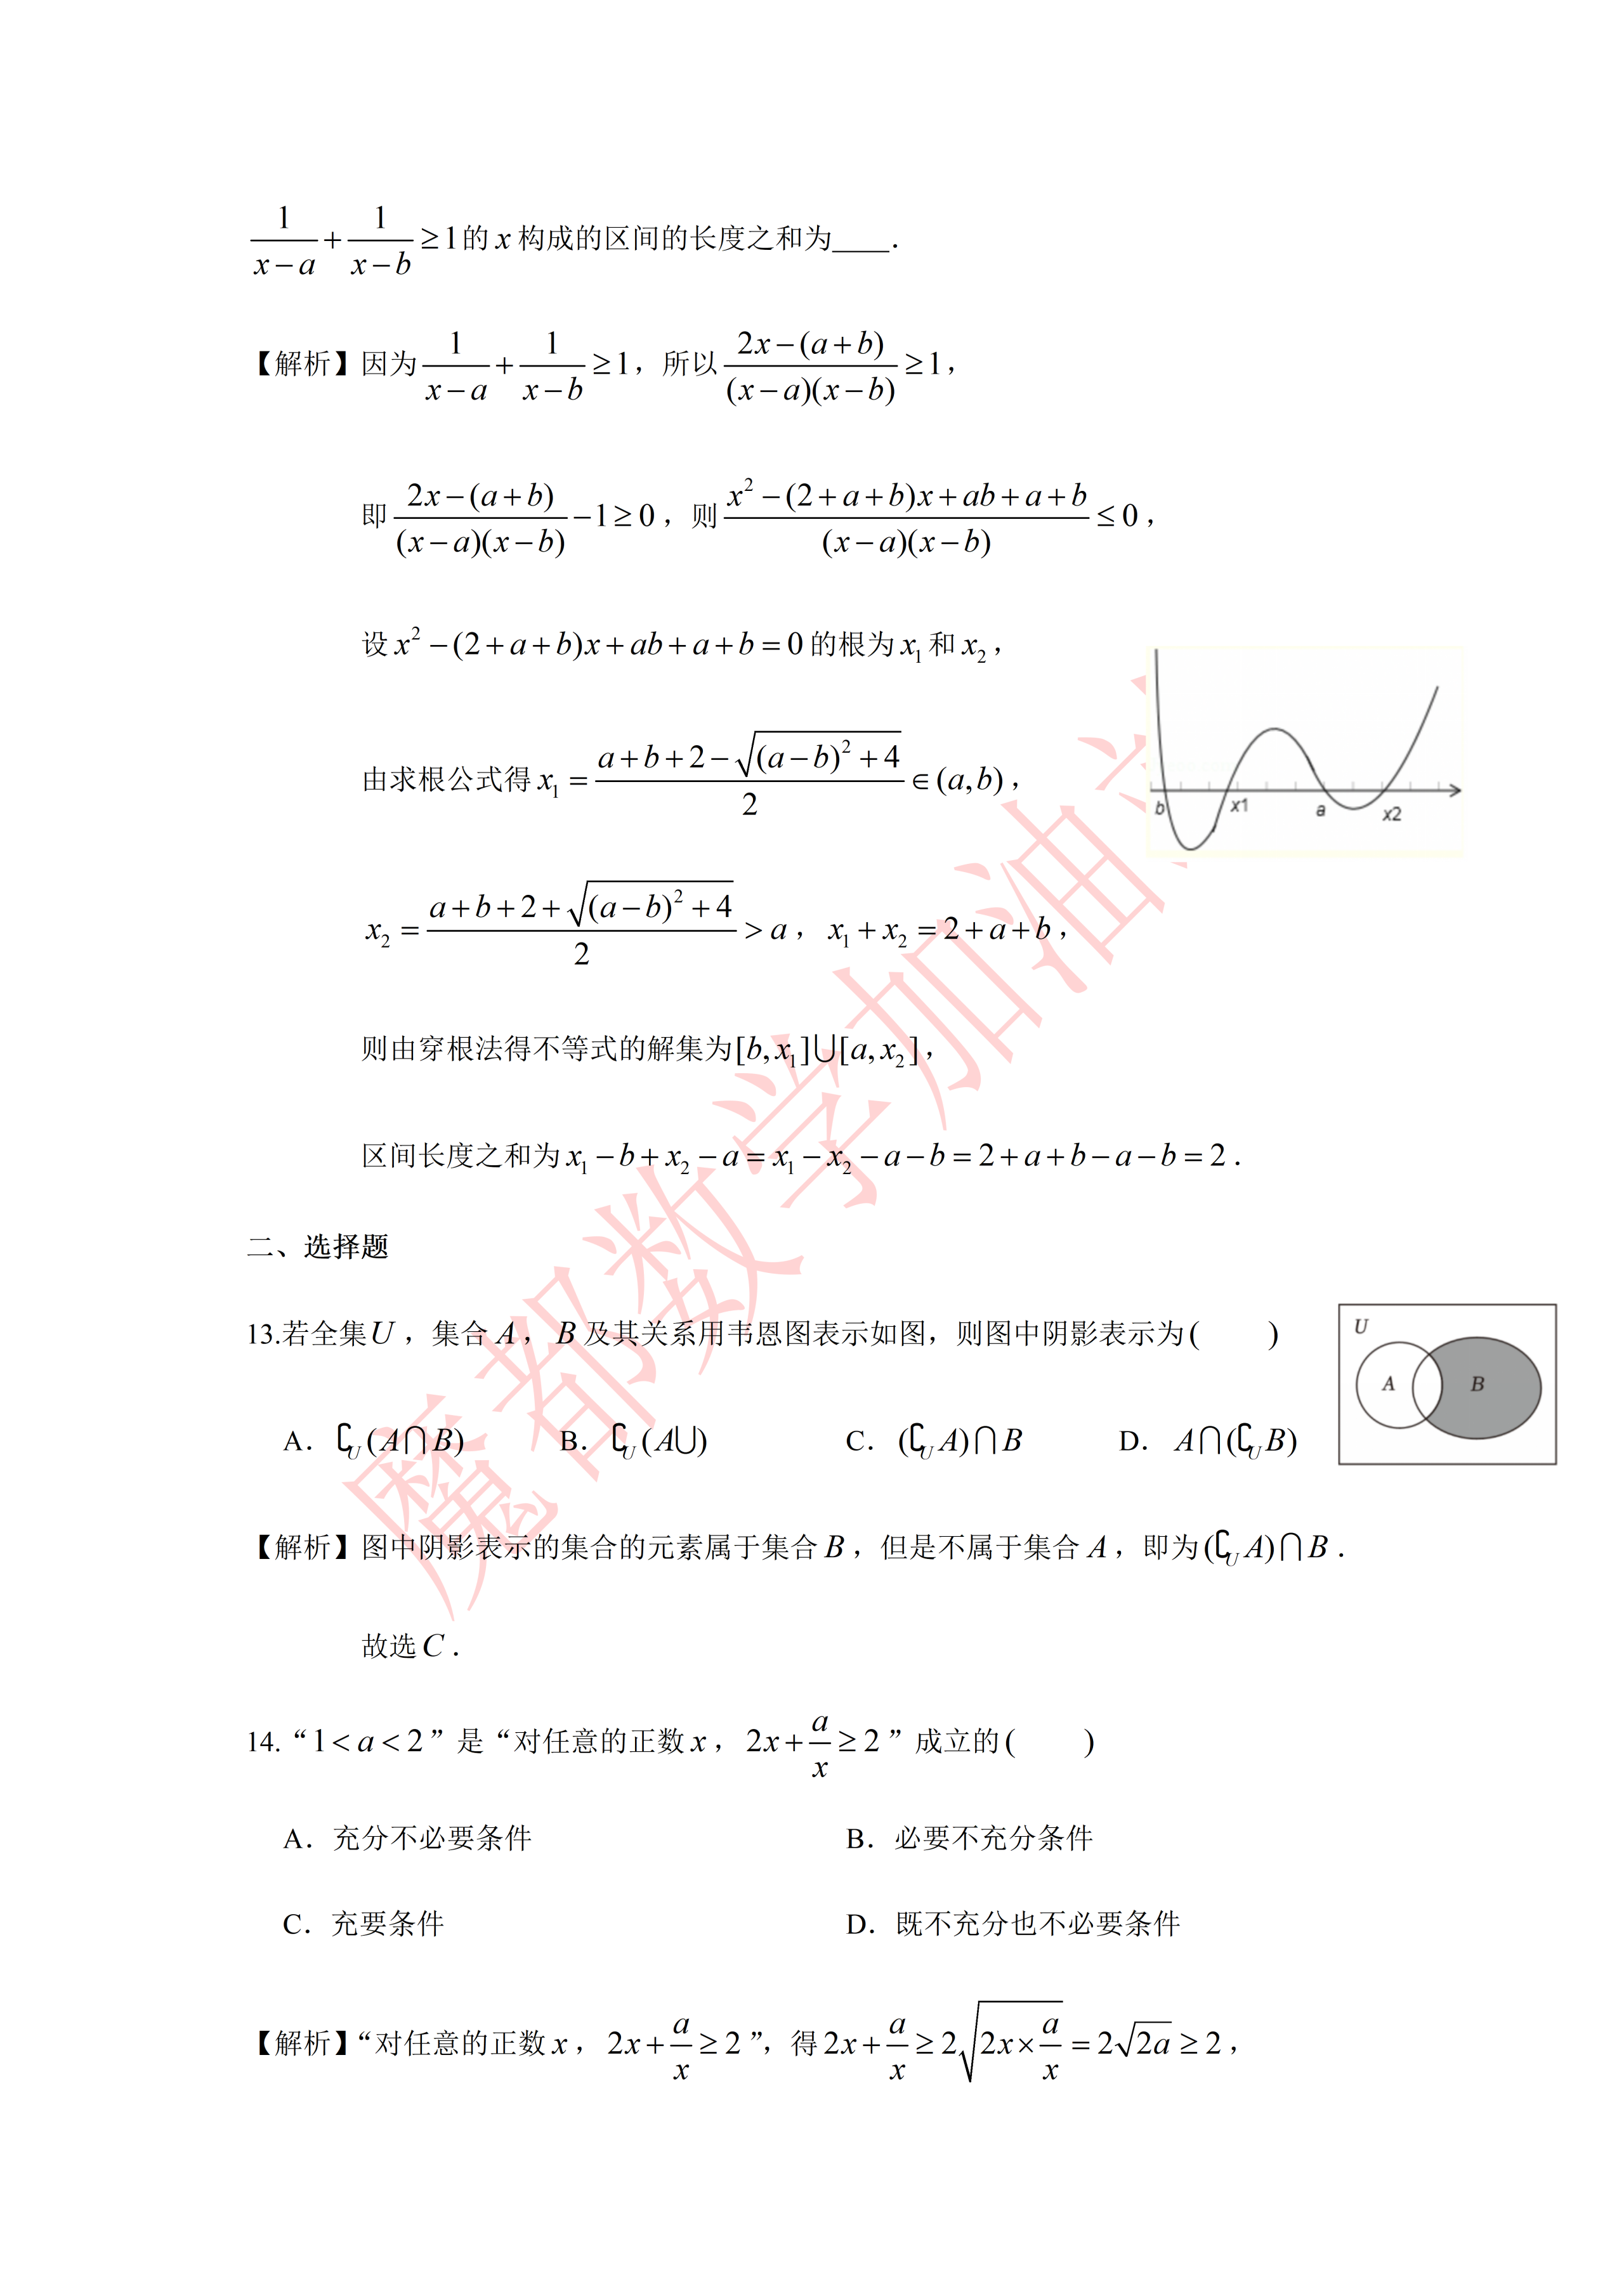
\includegraphics[width=.50\linewidth,trim=1786bp 2255bp 228bp 985bp,clip]{../原图/高一51_华师大二附中_国庆作业3/04.png}
\end{center}
\step{由求根公式得 $x_1=\dfrac{a+b+2-\sqrt{(a-b)^2+4}}{2}\in(a,b)$，}
\step{$x_2=\dfrac{a+b+2+\sqrt{(a-b)^2+4}}{2}>a$，$x_1+x_2=2+a+b$，}
\step{则由穿根法得不等式的解集为 $[b,x_1]\cup[a,x_2]$，}
% 原卷如此，照录未改（此处原卷作 $x_1-x_2$，按上一行 $x_1+x_2=2+a+b$ 当为 $x_1+x_2$）
\step{区间长度之和为 $x_1-b+x_2-a=x_1-x_2-a-b=2+a+b-a-b=2$.}
\solend

\fi

\end{enumerate}

\bigsec{二、选择题}

\begin{enumerate}
\setcounter{enumi}{12}

% 本题是“题干 + 图 + 选项”约 5.5cm 的一整块，图夹在题干与选项之间时 \keepwithprev 挡不住断点，
% 故按 高一30 第 13 题的成例在题前先量一次页高（守卫放在 \item 之前）。
\needvspace{6cm}
\item 若全集 $U$，集合 $A$、$B$ 及其关系用韦恩图表示如图，则图中阴影表示为\mbox{（\quad）}

\begin{center}
% 原卷该图印在题干与选项右侧（原图第 04 页），本稿移作居中排，直接裁取原图，不另存图片文件。
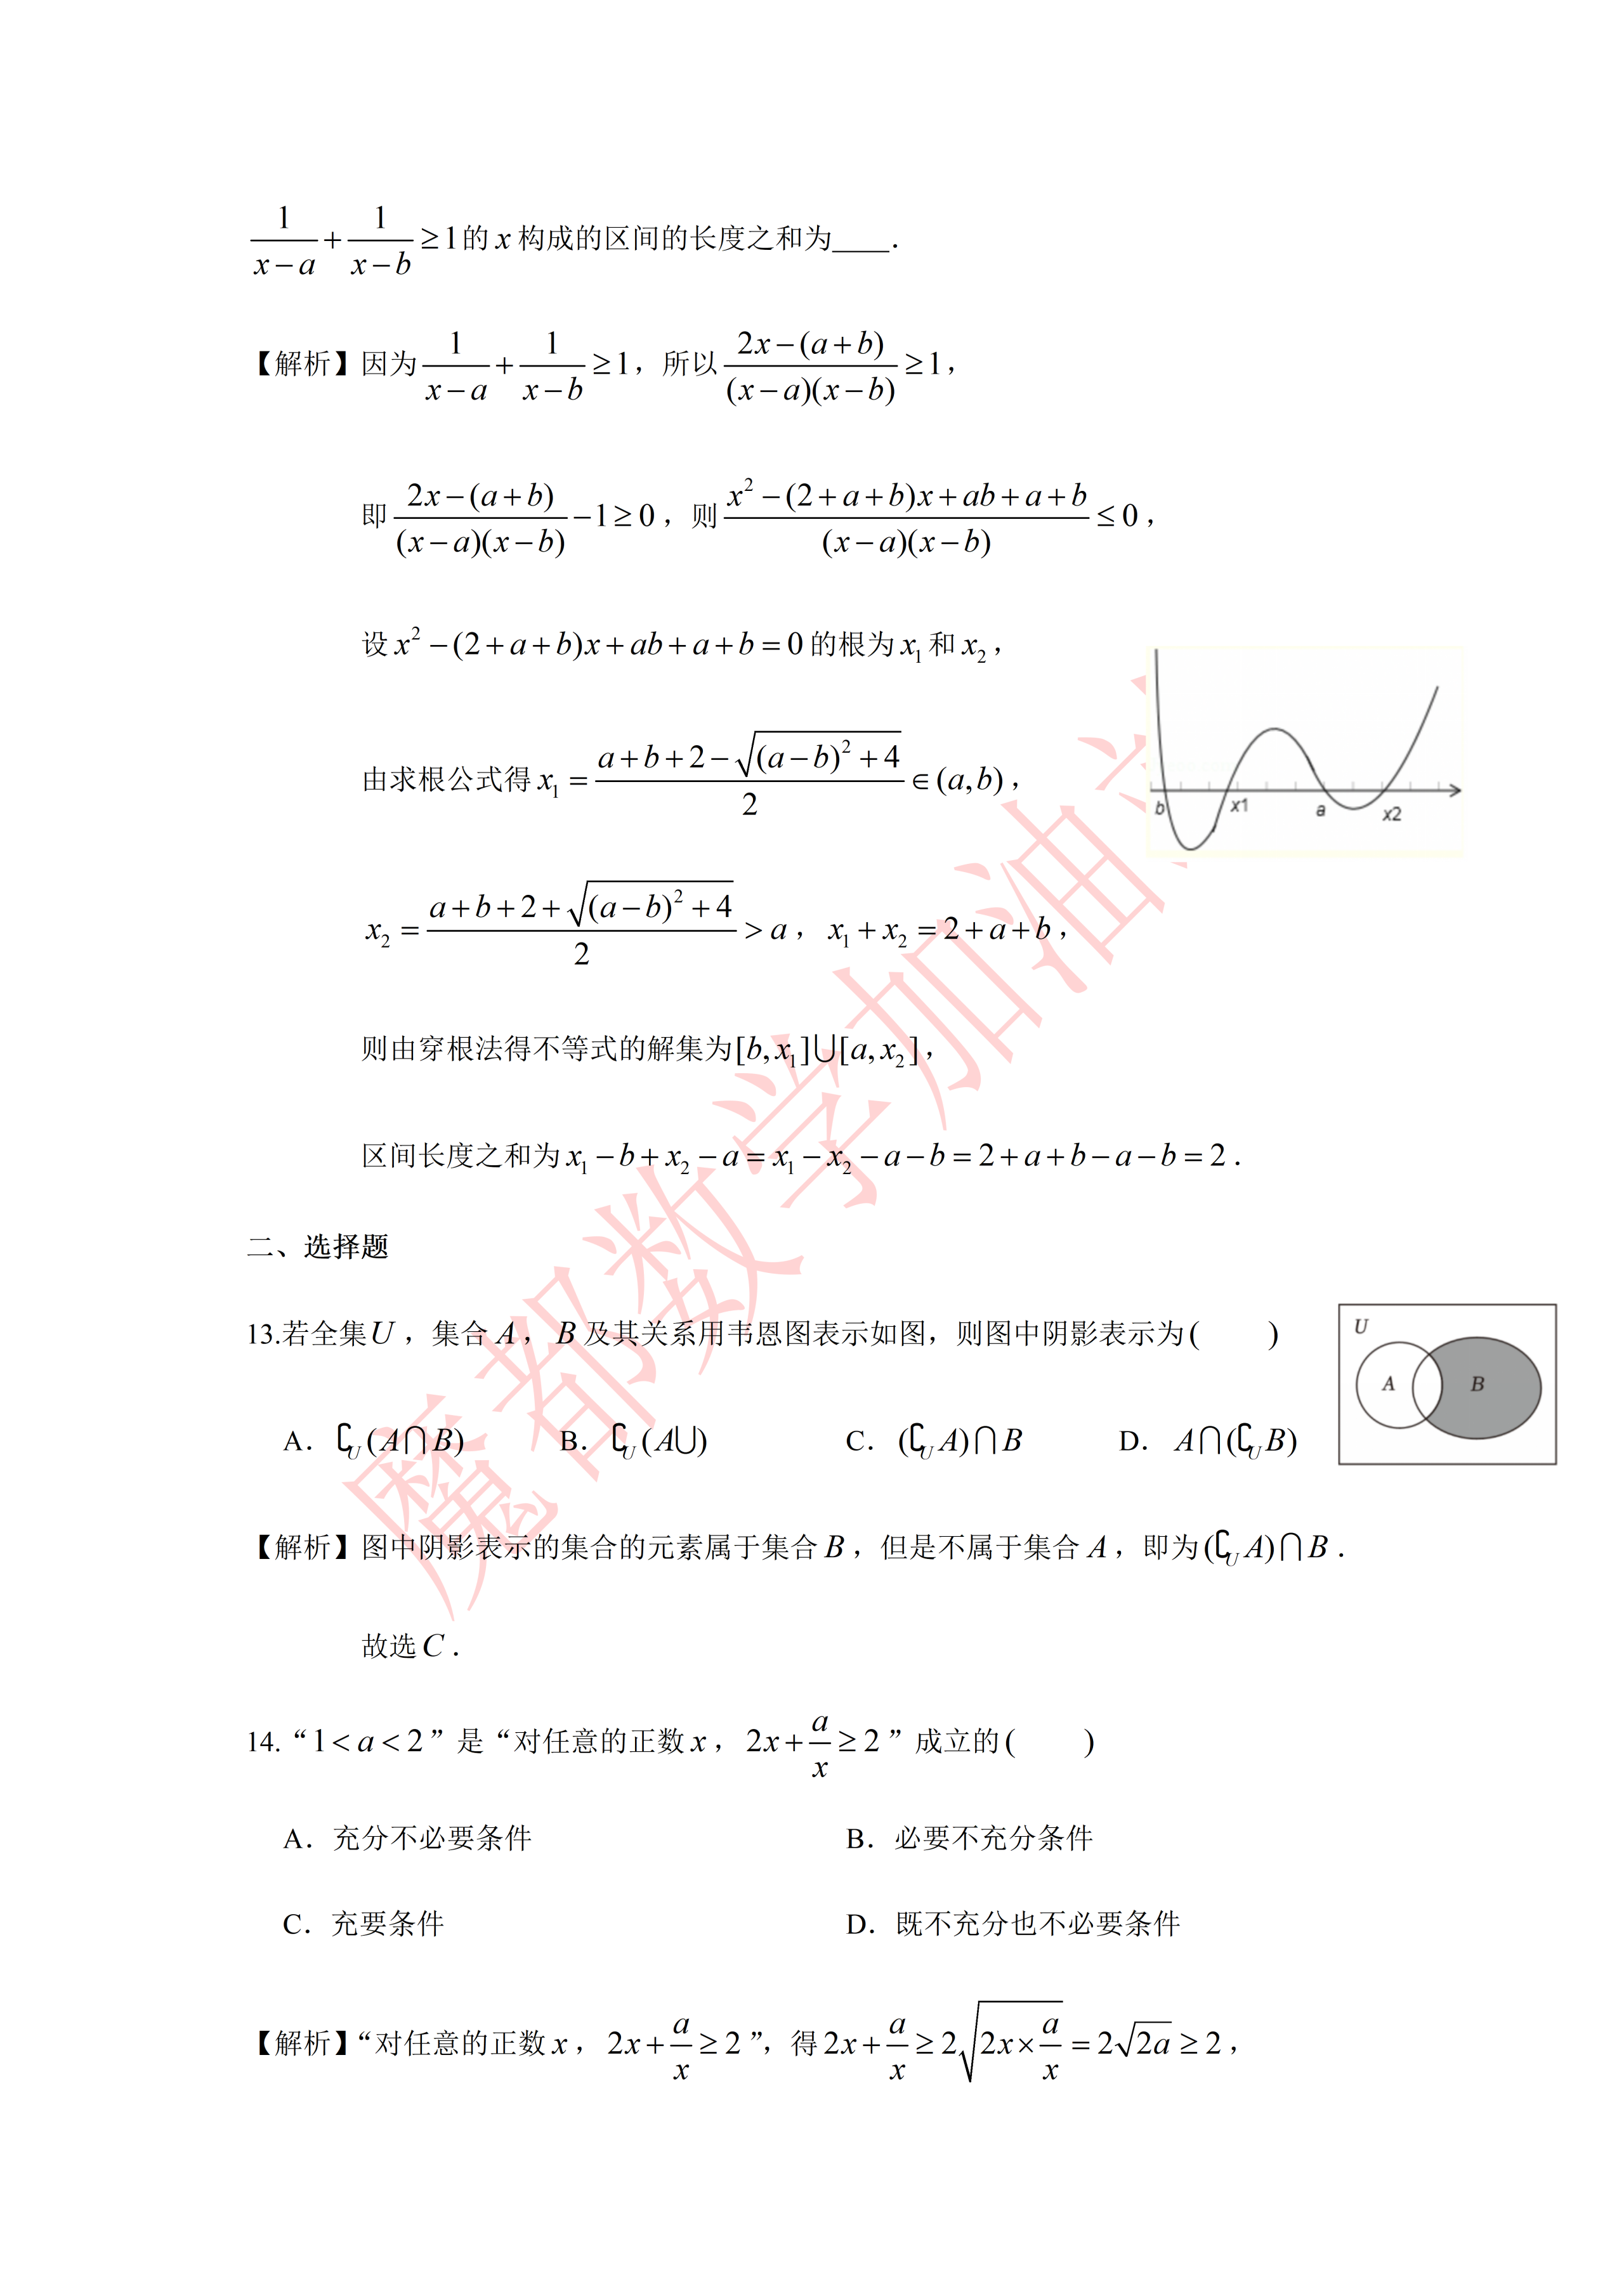
\includegraphics[width=.30\linewidth,trim=2105bp 1308bp 105bp 2050bp,clip]{../原图/高一51_华师大二附中_国庆作业3/04.png}
\end{center}

\keepwithprev
A. $\complement_U(A\cap B)$\qquad B. $\complement_U(A\cup B)$

C. $(\complement_U A)\cap B$\qquad D. $A\cap(\complement_U B)$

\ifanswer
\solbegin
\step{图中阴影表示的集合的元素属于集合 $B$，但是不属于集合 $A$，即为 $(\complement_U A)\cap B$.}
\step{故选 $C$.}
\solend

\fi

\item “$1<a<2$”是“对任意的正数 $x$，$2x+\dfrac ax\geqslant2$”成立的\mbox{（\quad）}

\keepwithprev
A. 充分不必要条件\qquad B. 必要不充分条件

C. 充要条件\qquad\qquad D. 既不充分也不必要条件

\ifanswer
\solbegin
\step{“对任意的正数 $x$，$2x+\dfrac ax\geqslant2$”，得 $2x+\dfrac ax\geqslant2\sqrt{2x\times\dfrac ax}=2\sqrt{2a}\geqslant2$，}
\step{所以 $\sqrt{2a}\geqslant1$，解得 $a\geqslant\dfrac12$，}
\step{若“$1<a<2$”得 $2x+\dfrac ax\geqslant2\sqrt{2x\times\dfrac ax}=2\sqrt{2a}>2\sqrt2>2$，}
\step{所以“$1<a<2$”$\Rightarrow$“对任意的正数 $x$，$2x+\dfrac ax\geqslant2$”，}
\step{所以“$1<a<2$”是“对任意的正数 $x$，$2x+\dfrac ax\geqslant2$”成立的充分不必要条件，}
\step{故选 $A$.}
\solend

\fi

\item 已知函数 $f(x)=2x-3$，$x\in(0,2)$，实数 $a$、$b$ 满足 $f(a)+f(b-1)=0$，则以下成立的有\mbox{（\quad）}

\keepwithprev
A. $a(b-1)$ 的最大值为 $\dfrac94$\qquad\qquad B. $b-\dfrac1a$ 的最大值为 $2$

C. $\dfrac1a+\dfrac1{4b}$ 的最小值为 $\dfrac9{16}$\qquad D. $-1<b-a<3$

\ifanswer
\solbegin
\step{因为函数 $f(x)=2x-3$，$x\in(0,2)$，实数 $a$、$b$ 满足 $f(a)+f(b-1)=0$，}
\step{所以 $2a-3+2(b-1)-3=0$，得 $a+b=4$，$a\in(0,2)$，$b\in(1,3)$，}
\step{所以 $a(b-1)=a(3-a)=-\left(a-\dfrac32\right)^2+\dfrac94$，$a\in(0,2)$，}
\step{所以 $0<a(b-1)\leqslant\dfrac94$，故选项 $A$ 正确；}
\step{$b-\dfrac1a=4-a-\dfrac1a=4-\left(a+\dfrac1a\right)\leqslant4-2=2$，}
\step{当且仅当 $a=1$，$b=3$ 时取等号，又 $b\in(1,3)$，故 $b-\dfrac1a<2$，故 $B$ 错误；}
\step{$\dfrac1a+\dfrac1{4b}=\dfrac14\left(\dfrac1a+\dfrac1{4b}\right)(a+b)=\dfrac14\left(1+\dfrac14+\dfrac ba+\dfrac a{4b}\right)=\dfrac5{16}+\dfrac14\left(\dfrac ba+\dfrac a{4b}\right)$}
\step{$\geqslant\dfrac5{16}+\dfrac14\cdot2\sqrt{\dfrac ba\cdot\dfrac a{4b}}=\dfrac9{16}$，当且仅当 $\dfrac ba=\dfrac a{4b}$，即 $a=2b=\dfrac83$ 时取等号，}
% 原卷如此，照录未改（“又 $a\in(0,2)$，”与下式之间原卷正文夹印“水印”二字）
\step{又 $a\in(0,2)$，水印 $\dfrac1a+\dfrac1{4b}<\dfrac9{16}$，故 $C$ 错误；}
\step{因为 $a\in(0,2)$，$b\in(1,3)$，所以 $-a\in(-2,0)$，所以 $b-a\in(-1,3)$，}
\step{故 $D$ 正确；}
\step{故选 $AD$.}
\solend

\fi

% 本题解析含图（“函数 f(x) 的图像如下”），图夹在解析行间，页末放不下会被拆开，
% 故在题前先量一次页高；上界取“题干 + 选项 + 图 + 首行解析”一块的高度。
\needvspace{6cm}
\item 设 $M_I$ 表示函数 $f(x)=|x^2-4x+2|$ 在闭区间 $I$ 上的最大值. 若正实数 $a$ 满足
$M_{[0,a]}\geqslant2M_{[a,2a]}$，则正实数 $a$ 的取值范围是\mbox{（\quad）}

\keepwithprev
A. $\left[2-\sqrt3,\dfrac12\right]$\qquad B. $[2-\sqrt3,1]$

C. $[2,2+\sqrt3]$\qquad\qquad D. $[2+\sqrt3,4]$

\ifanswer
\solbegin
\step{函数 $f(x)$ 的图像如下：}
\begin{center}
% 原卷该图印在解析行间（原图第 06 页），本稿直接裁取原图，不另存图片文件。
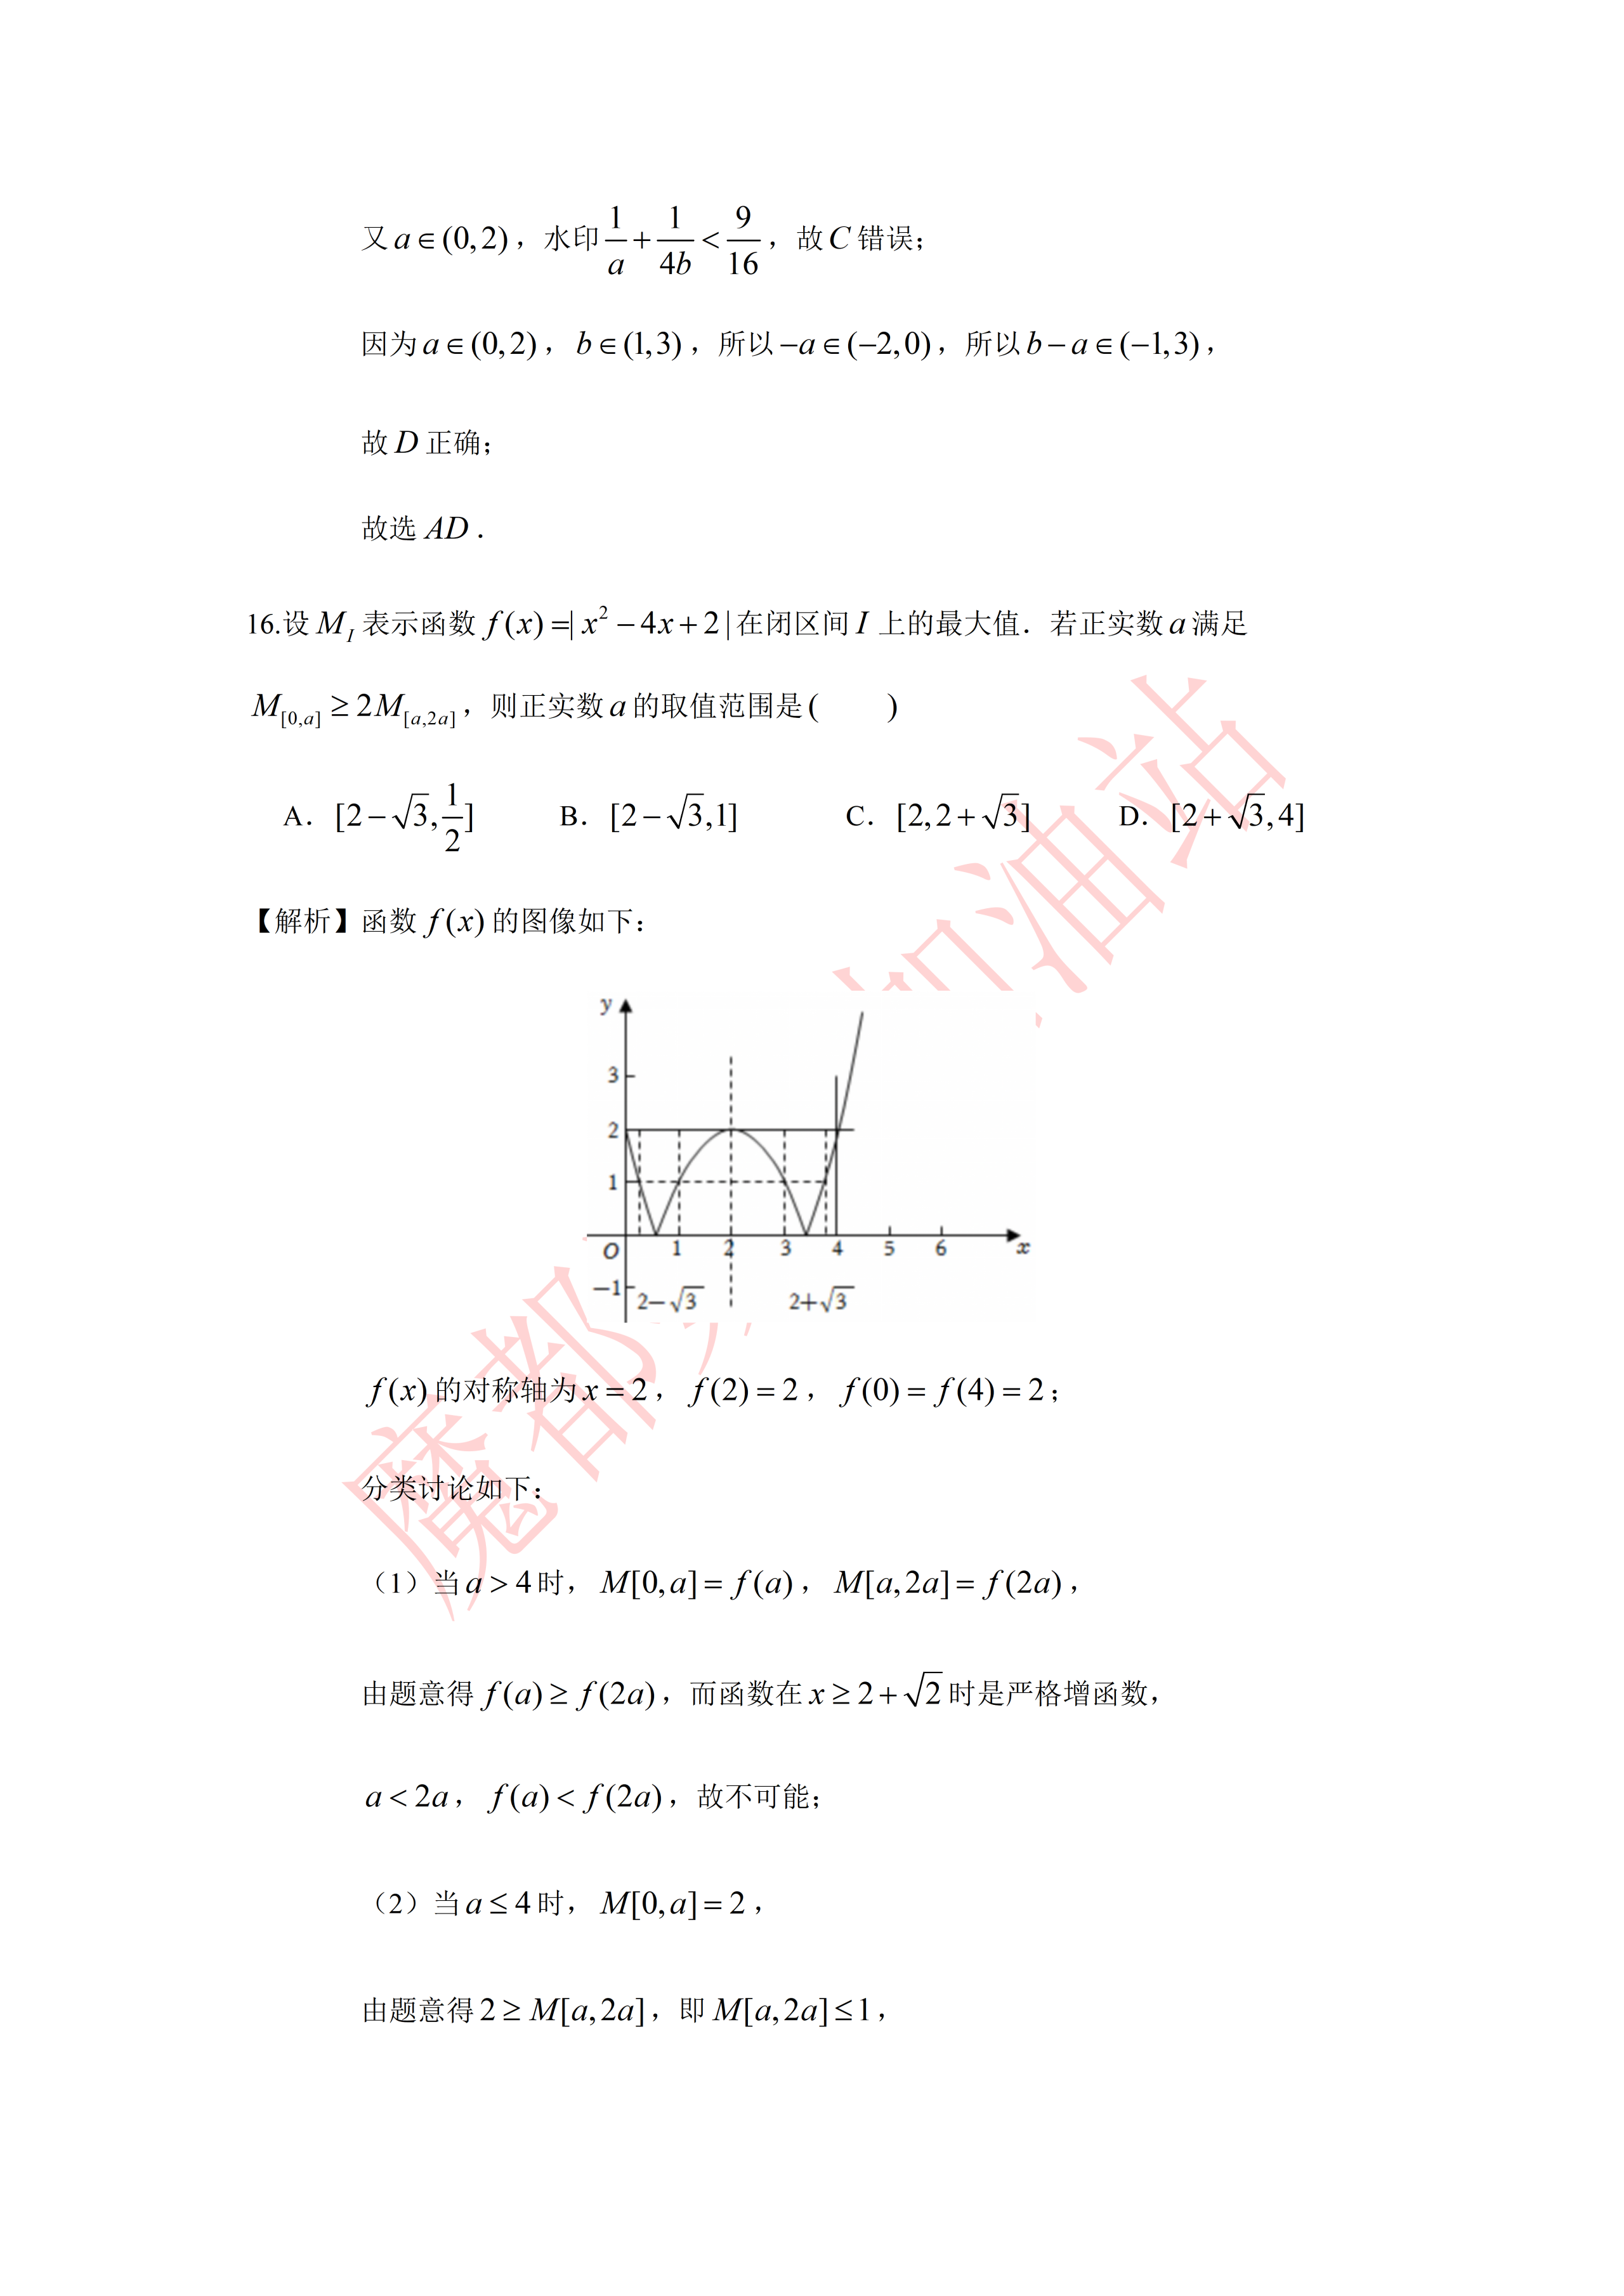
\includegraphics[width=.55\linewidth,trim=895bp 1535bp 915bp 1525bp,clip]{../原图/高一51_华师大二附中_国庆作业3/06.png}
\end{center}
\step{$f(x)$ 的对称轴为 $x=2$，$f(2)=2$，$f(0)=f(4)=2$；}
\step{分类讨论如下：}
\stepm{(1)}{当 $a>4$ 时，$M_{[0,a]}=f(a)$，$M_{[a,2a]}=f(2a)$，}
\step{由题意得 $f(a)\geqslant f(2a)$，而函数在 $x\geqslant2+\sqrt2$ 时是严格增函数，}
\step{$a<2a$，$f(a)<f(2a)$，故不可能；}
\stepm{(2)}{当 $a\leqslant4$ 时，$M_{[0,a]}=2$，}
\step{由题意得 $2\geqslant M_{[a,2a]}$，即 $M_{[a,2a]}\leqslant1$，}
\step{令 $f(x)=1$，解得 $x_1=2-\sqrt3$，$x_2=1$，$x_3=2+\sqrt3$，$x_4=3$，}
\step{则有 $a\geqslant2-\sqrt3$ 并且 $2a\leqslant1$，解得 $2-\sqrt3\leqslant a\leqslant\dfrac12$；}
\step{或者 $a\geqslant3$ 并且 $2a\leqslant2+\sqrt3$，无解；}
\step{故选 $A$.}
\solend

\fi

\end{enumerate}

\bigsec{三、解答题}

\begin{enumerate}
\setcounter{enumi}{16}

\item 已知 $M=\{x\mid2\leqslant x\leqslant5\}$，$N=\{x\mid a-1\leqslant x\leqslant2a+1\}$.
\begin{enumerate}[label=(\arabic*)]
\item 若 $M\subseteq N$，求实数 $a$ 的取值范围；
\item 若 $M\supseteq N$，求实数 $a$ 的取值范围.
\end{enumerate}

\ifanswer
\ans{（1）$[2,3]$；（2）$(-\infty,-2)$}
\fi

\ansspace[6]

\item 设集合 $A=\{x\mid|x+1|\leqslant3\}$，$B=\{x\mid0<x<3m\}$.
\begin{enumerate}[label=(\arabic*)]
\item 若 $A\cup B=A$，求实数 $m$ 的取值范围；
\item 设 $P=(\complement_R A)\cap B$，若 $\exists x\in\Z$ 且 $x\in P$，求实数 $m$ 的取值范围.
\end{enumerate}

\ifanswer
\solbegin
\stepm{(1)}{$A=\{x\mid|x+1|\leqslant3\}=\{x\mid-4\leqslant x\leqslant2\}$，且 $A\cup B=A$，所以 $B\subseteq A$.}
\step{若 $B=\varnothing$，此时 $0\geqslant3m$，解得 $m\leqslant0$；}
\step{若 $B\neq\varnothing$，此时 $0<3m$，且 $3m\leqslant2$，解得 $0<m\leqslant\dfrac23$；}
\step{则实数 $m$ 的取值范围是 $\left(-\infty,\dfrac23\right]$.}
\stepm{(2)}{因为 $\exists x\in\Z$ 且 $x\in P$，所以集合 $P$ 中至少存在一个整数.}
\step{$\complement_R A=\{x\mid x<-4\text{ 或 }x>2\}$，$B=\{x\mid0<x<3m\}$，}
\step{要使 $P=(\complement_R A)\cap B$ 中至少存在一个整数，则 $\begin{cases}3m>0\\3m>3\end{cases}$，解得 $m>1$，}
\step{则实数 $m$ 的取值范围是 $(1,+\infty)$.}
\solend

\fi

\ansspace[7]

\item 已知函数 $f(x)=x^2+(1-a)x-a(a\in\R)$.
\begin{enumerate}[label=(\arabic*)]
\item 解关于 $x$ 的不等式 $f(x)<0$；
\item 若 $\forall a\in[-1,1]$，$f(x)\geqslant0$ 恒成立，求实数 $x$ 的取值范围.
\end{enumerate}

\ifanswer
\solbegin
\stepm{(1)}{不等式 $x^2+(1-a)x-a<0$ 等价于 $(x-a)(x+1)<0$，}
\step{当 $a<-1$ 时，不等式的解集为 $(a,-1)$；}
\step{当 $a=-1$ 时，不等式的解集为 $\varnothing$；}
\step{当 $a>-1$ 时，不等式的解集为 $(-1,a)$.}
\stepm{(2)}{$x^2+(1-a)x-a=-a(x+1)+x^2+x$，}
\step{设 $g(a)=-a(x+1)+x^2+x$，$a\in[-1,1]$，}
\step{要使 $g(a)\geqslant0$ 在 $a\in[-1,1]$ 上恒成立，}
\step{只需 $\begin{cases}g(-1)\geqslant0\\g(1)\geqslant0\end{cases}$，即 $\begin{cases}x^2+2x+1\geqslant0\\x^2-1\geqslant0\end{cases}$，解得 $x\geqslant1$ 或 $x\leqslant-1$，}
\step{所以 $x$ 的取值范围为 $\{x\mid x\leqslant-1\text{ 或 }x\geqslant1\}$.}
\solend

\fi

\ansspace[7]

\item 若实数 $x$、$y$、$m$ 满足 $|x-m|>|y-m|$，则称 $x$ 比 $y$ 远离 $m$.
\begin{enumerate}[label=(\arabic*)]
\item 若 $2$ 比 $3x-4$ 远离 $1$，求 $x$ 的取值范围；
\item 设 $y=\dfrac{x+2}{x+1}$，其中 $x\in(0,\sqrt2)\cup(\sqrt2,+\infty)$，判断：$x$ 与 $y$ 哪一个更远离 $\sqrt2$？并说明理由.
\item 若 $x+y=2$，试问：$y$ 与 $x^2+y^2$ 哪一个更远离 $\dfrac12$？并说明理由.
\end{enumerate}

\ifanswer
\solbegin
\stepm{(1)}{由题意得 $|2-1|>|3x-4-1|$，所以 $|3x-5|<1$，解得 $\dfrac43<x<2$，}
\step{故 $x$ 的取值范围为 $\left(\dfrac43,2\right)$；}
\stepm{(2)}{$x$ 比 $y$ 更远离 $\sqrt2$，}
\step{理由如下：要证 $x$ 比 $y$ 更远离 $\sqrt2$，只要证 $|x-\sqrt2|>\left|\dfrac{x+2}{x+1}-\sqrt2\right|$，}
\step{即证 $|x-\sqrt2|>\left|\dfrac{(1-\sqrt2)(x-\sqrt2)}{x+1}\right|$，}
\step{因为 $x\in(0,\sqrt2)\cup(\sqrt2,+\infty)$，所以 $|x-\sqrt2|>0$，}
\step{所以只要证 $1>\dfrac{\sqrt2-1}{|x+1|}$，即证 $|x+1|>\sqrt2-1$，}
\step{因为 $x\in(0,\sqrt2)\cup(\sqrt2,+\infty)$，所以 $x+1\in(1,\sqrt2+1)\cup(\sqrt2+1,+\infty)$，}
\step{所以 $|x+1|>1>\sqrt2-1$，所以 $x$ 比 $y$ 更远离 $\sqrt2$；}
\stepm{(3)}{因为 $x^2+y^2\geqslant\dfrac{(x+y)^2}{2}=2$，当且仅当 $x=y=1$ 时等号成立，}
\step{所以 $\left|x^2+y^2-\dfrac12\right|=x^2+y^2-\dfrac12$，}
\step{从而 $\left|y-\dfrac12\right|-\left|x^2+y^2-\dfrac12\right|=\left|y-\dfrac12\right|-\left(x^2+y^2-\dfrac12\right)$，}
\step{①$y\geqslant\dfrac12$，$\left|y-\dfrac12\right|-\left|x^2+y^2-\dfrac12\right|=y-\dfrac12-\left(x^2+y^2-\dfrac12\right)=y-x^2-y^2$}
\step{$=y-(2-y)^2-y^2=-2y^2+5y-4=-2\left(y-\dfrac54\right)^2-\dfrac78<0$，}
\step{即 $\left|y-\dfrac12\right|<\left|x^2+y^2-\dfrac12\right|$；}
\step{②$y<\dfrac12$，}
\step{$\left|y-\dfrac12\right|-\left|x^2+y^2-\dfrac12\right|=\left(\dfrac12-y\right)-\left(x^2+y^2-\dfrac12\right)=-y-x^2-y^2+1$}
\step{$=-y-(2-y)^2-y^2+1=-2y^2+3y-3=-2\left(y-\dfrac34\right)^2-\dfrac{15}8<0$，}
\step{即 $\left|y-\dfrac12\right|<\left|x^2+y^2-\dfrac12\right|$；}
\step{综上，$\left|y-\dfrac12\right|<\left|x^2+y^2-\dfrac12\right|$，即 $x^2+y^2$ 比 $y$ 更远离 $\dfrac12$.}
\solend

\fi

\ansspace[9]

\item 对于非空有限整数集 $X$，$m\in\N^*$，定义 $X^m=\{x^m\mid x\in X\}$，对 $n\in\Z$，
$Y\oplus n=\{x+n\mid x\in Y\}$ 现有两个非空有限整数集 $A$、$B$，已知 $A\oplus1\subseteq B$ 且
$B^2\oplus(-4)\subseteq A$.
\begin{enumerate}[label=(\arabic*)]
\item 当 $A=\{-3,0\}$ 时求集合 $B$；
\item 证明：$A\subseteq\{-3,-2,0,1\}$；
\item 当 $A\oplus1=B$ 且 $B^2\oplus(-4)=A$ 时，任取 $a\in A$，$b\in B$ 构造函数
$f(x)=(x-a)(x-b)$ 问：当 $a$、$b$ 取何值时，$f(x)$ 的最小值最小？
\end{enumerate}

\ifanswer
\solbegin
\stepm{(1)}{因为 $A=\{-3,0\}$，$B^2\oplus(-4)\subseteq A$，}
\step{所以 $B^2\oplus(-4)$ 可能为 $\varnothing$、$\{-3\}$、$\{0\}$、$\{-3,0\}$，}
\step{当 $B^2\oplus(-4)=\varnothing$ 时 $B^2=\varnothing$，不满足非空，不合题意；}
\step{当 $B^2\oplus(-4)=\{-3\}$ 时 $B^2=\{1\}$，所以 $B=\{1,-1\}$、$\{1\}$、$\{-1\}$，}
\step{当 $B^2\oplus(-4)=\{0\}$ 时 $B^2=\{4\}$，所以 $B=\{2,-2\}$、$\{2\}$、$\{-2\}$，}
% 原卷如此，照录未改（此处作 $\{0,-3\}$，上一行同一集合作 $\{-3,0\}$）
\step{当 $B^2\oplus(-4)=\{0,-3\}$ 时 $B^2=\{4,1\}$，}
\step{所以 $B=\{1,2,-1,-2\}$、$\{2,-1,-2\}$、$\{2,1,-2\}$、$\{1,-1,-2\}$、$\{1,-1,2\}$、$\{1,2\}$、$\{-1,2\}$、$\{-1,-2\}$、$\{1,-2\}$，}
\step{又 $A\oplus1=\{-2,1\}\subseteq B$，得 $B$ 为 $\{1,-2\}$、$\{2,1,-2\}$、$\{1,-1,-2\}$、$\{1,2,-1,-2\}$.}
\stepm{(2)}{设 $x\in A$，因为 $A\oplus1\subseteq B$，所以 $x+1\in B$，}
\step{又 $B^2\oplus(-4)\subseteq A$，所以 $(x+1)^2-4\in A$，}
% 原卷如此，照录未改（此处及下文取 $x=2$ 处原卷均作 $(-4+1)^2-4=52-2a>0$）
\step{取 $x=-4$，则 $(-4+1)^2-4=52-2a>0$，$(5+1)^2-4=32\in A$，$\cdots$，}
\step{无限迭代，而 $A$ 为有限集，不合题意，舍去，即 $-4\notin A$；}
\step{取 $x=-3$，则 $(-3+1)^2-4=0\in A$，$(0+1)^2-4=-3\in A$，}
\step{得 $A$ 集合可为 $\{-3,0\}$；}
\step{取 $x=-2$，则 $(-2+1)^2-4=-3\in A$，$(-3+1)^2-4=0\in A$，}
\step{$(0+1)^2-4=-3\in A$，得 $A$ 集合可为 $\{-3,-2,0\}$；}
\step{取 $x=-1$，则 $(-1+1)^2-4=-4\in A$，又 $-4\notin A$，所以 $-1\notin A$，}
\step{取 $x=1$，则 $(1+1)^2-4=0\in A$，$(0+1)^2-4=-3\in A$，}
\step{$(-3+1)^2-4=0\in A$，得 $A$ 集合可为 $\{-3,0,1\}$，}
\step{取 $x=2$，则 $(2+1)^2-4=52-2a>0$，$(5+1)^2-4=32\in A$，$\cdots$，}
\step{无限迭代，而 $A$ 为有限集，不合题意，舍去，即 $2\notin A$，}
\step{同理当 $x<-4$ 或 $x>2$，且 $x\in\Z$ 时不符合 $A$ 为有限集，舍去；}
\step{故由上得 $A$ 集合可为 $\{-3,0\},\{-3,-2,0\},\{-3,0,1\},\{-3,-2,0,1\}$，}
\step{所以 $A\subseteq\{-3,-2,0,1\}$，}
\stepm{(3)}{当 $A\oplus1=B$ 且 $B^2\oplus(-4)=A$ 时，}
\step{设 $x\in B$，则 $x^2-4\in B^2\oplus(-4)=A$，}
% 原卷如此，照录未改（题设 $A=\{-3,0\}$，此处两个判别式取的是 $-2$ 与 $1$，均不属于 $A$）
\step{$x^2-4=-2$ 时 $x=\pm\sqrt2$，不为整数，不合题意；}
\step{$x^2-4=1$ 时 $x=\pm\sqrt5$，不为整数，不合题意；}
\step{所以 $A=\{-3,0\}$，又 $A\oplus1=B$，则 $B=\{-2,1\}$，}
\step{任取 $a\in A$，$b\in B$ 构造函数 $f(x)=(x-a)(x-b)$，}
\step{$f(x)=(x-a)(x-b)=x^2-(a+b)x+ab$}
\step{$=x^2-(a+b)x+\dfrac{(a+b)^2}{4}+ab-\dfrac{(a+b)^2}{4}$}
\step{$=\left[x-\dfrac{(a+b)}2\right]^2-\dfrac{(a-b)^2}{4}\geqslant-\dfrac{(a-b)^2}{4}$，所以 $f(x)_{min}=-\dfrac{(a-b)^2}{4}$，}
\step{又 $a\in A=\{-3,0\}$，$b\in B=\{-2,1\}$，所以 $a-b$ 的取值有 $-1,-4,2$，}
\step{所以 $f(x)_{min}=-\dfrac{(a-b)^2}{4}\geqslant-\dfrac{(-3-1)^2}{4}=-4$，}
\step{即当 $a=-3$，$b=1$ 时 $f(x)_{min}$ 的最小值为 $-4$.}
\solend

\fi

\ansspace*[12]

\end{enumerate}

\end{document}
"
%
% 原始材料：微信公众号“魔都数学加油站”文章，作者破晓，连载“27学年高一51”；
% 原文标题“27学年高一51——2026-2027年上海市华师大二附中高一上国庆作业3”；
% 原文链接：https://mp.weixin.qq.com/s/95SLMEmPUT30s4U7wjr5Og。
% 该页面用 JS 渲染，未见明确发布日期；页面内时间戳约为 2026-10-05 21:37，本稿以该时刻记可得日期。
% 正文为 12 张 PNG 页：第 01、02、03、05、07、08、11 页 4762×6735，
% 第 04、06、09、10、12 页 2560×3620。按页序逐页读取，12 页全为试卷正文页
% （卷首标题在第 1 页页顶，卷末解答题止于第 12 页），无封面页、目录页或单独的页脚页。
% 卷面标题照原卷印作“2026-2027 年华师大二附中高一上国庆作业 3”（公众号标题中的“上海市”
% 卷面标题行没有，本稿照卷面），年份区间按全稿惯例排 en dash。
%
% 篇幅与题号：原卷自第 3 题起编号（第 1、2 题不在本卷内）。填空题 3—12（10 题）、
% 选择题 13—16（4 题）、解答题 17—21（5 题），共 19 题。本稿沿用原节与原题号，
% 只改排为全稿统一的大节样式（原卷小节标题为“一、填空题”“二、选择题”“三、解答题”）。
% 正文为讲评版：填空题 3—12 与选择题 13—16 只印【解析】（选择题的结论“故选 X”印在解析内），
% 按全稿口径这类题不另提 \ans{}；解答题第 17 题只印【答案】，故只给 \ans{}；
% 第 18—21 题只印【解析】。
%
% 副标题：原卷未印副标题。本稿按“知识模块”口径标作“集合与常用逻辑用语、不等式”：
% 19 题中集合与常用逻辑用语 8 题（3、4、6、10、13、17、18、21），
% 不等式（含函数最值、绝对值不等式）11 题（5、7、8、9、11、12、14、15、16、19、20），
% 两类均远超三分之一，故并标。口径同 高一46_交附闵行_国庆作业3、高一48_华师大二附中_周末作业2。
%
% 与原卷的排版差异：
%   ① 原卷每题下直接印【答案】或【解析】，本稿按全稿惯例将答案与解析置于答案版；
%   ② 原卷未印副标题，本稿按“知识模块”口径补出；
%   ③ 原卷填空横线按全稿惯例排为 \blankline[4.4em]；
%   ④ 原卷 $R$、$N$、$Z$ 均排斜体，本稿按全稿惯例改用花体 $\R$、$\N$、$\Z$（同 高一48）；
%   ⑤ 原卷第 12 题解析配图、第 13 题题干韦恩图都印在正文右侧的浮动位置，第 16 题解析配图
%      印在解析行间；本稿三图一律居中排，均自原图对应页裁切（trim），不另存图片文件；
%   ⑥ 原卷解答题未留作答空白，本稿按全稿惯例加 \ansspace；
%   ⑦ 原卷第 15 题解析第 7、8 两个印刷行是一串连等式的折行，本稿按“一条 \step ＝ 一个印刷行”
%      的口径分成两条 \step。
%
% 原卷笔误/存疑（均照录未改，正文对应处另有 % 注）：
%   ① 第 12 题解析末行作“区间长度之和为 $x_1-b+x_2-a=x_1-x_2-a-b=2+a+b-a-b=2$”，
%      按上一行 $x_1+x_2=2+a+b$，此处应为 $x_1+x_2$；原卷作 $x_1-x_2$。
%   ② 第 15 题解析“又 $a\in(0,2)$，”与 $\dfrac1a+\dfrac1{4b}<\dfrac9{16}$ 之间，
%      原卷正文夹印“水印”二字（系制版遗留字样，非试卷内容）。
%   ③ 第 21 题第 (2) 问解析两处（取 $x=-4$、取 $x=2$）作“$=52-2a>0$”，
%      与题设 $(x+1)^2-4$ 的取值（按 $x=-4$ 应为 $5$）不符，当系原卷算式遗留。
%   ④ 第 21 题第 (1) 问解析先写 $B^2\oplus(-4)$ 可能为 $\{-3,0\}$，后文又作 $\{0,-3\}$，
%      同一集合两种写法。
%   ⑤ 第 21 题第 (3) 问解析：题设 $B^2\oplus(-4)=A$ 且 $A=\{-3,0\}$ 时，由 $x^2-4\in A$
%      应得 $x^2-4=-3$ 或 $0$；原卷讨论的却是 $x^2-4=-2$ 与 $x^2-4=1$（两值均不属于 $A$），
%      与题设不合。
%
% 插图：3 张，均自原图裁切（无 \begin{tikzpicture} 重排）：
%   · 第 13 题题干韦恩图（原图第 04 页，图在题干与选项右侧）
%   · 第 12 题解析配图（原图第 04 页，图在解析右侧）
%   · 第 16 题解析配图（原图第 06 页，图在解析中间）
%
\documentclass[a4paper,11pt]{article}
\usepackage{common}

\begin{document}

\examtitlest[3]{2026--2027 年华师大二附中高一上国庆作业 3}{集合与常用逻辑用语、不等式}

\bigsec{一、填空题}

\begin{enumerate}
\setcounter{enumi}{2}

\item 若 $\{x\mid x<1\text{ 或 }x>4\}\cup\{x\mid m<x<2m+3\}=R$，则实数 $m$ 的取值范围为\blankline[4.4em].

\ifanswer
\solbegin
\step{因为 $\{x\mid x<1\text{ 或 }x>4\}\cup\{x\mid m<x<2m+3\}=R$，}
\step{所以 $\begin{cases}m<1\\2m+3>4\end{cases}$，解得 $\dfrac12<m<1$，所以 $m$ 的取值范围为 $\left(\dfrac12,1\right)$.}
\solend

\fi

\item 若“$x\leqslant5$”是“$x<a$”的必要不充分条件，则 $a$ 的取值范围是\blankline[4.4em].

\ifanswer
\solbegin
\step{若“$x\leqslant5$”是“$x<a$”的必要不充分条件，则 $\{x\mid x<a\}\subset\{x\mid x\leqslant5\}$，}
\step{所以 $a\leqslant5$.}
\solend

\fi

\item 实数 $x$、$y$ 满足 $x^2+2xy+4y^2=1$，则 $x+2y$ 的取值范围是\blankline[4.4em].

\ifanswer
\solbegin
\step{因为 $x^2+2xy+4y^2=(x+2y)^2-2xy=1$，}
\step{所以 $(x+2y)^2-1=x\cdot(2y)\leqslant\left(\dfrac{x+2y}{2}\right)^2$，当且仅当 $x=2y$ 时取等号，}
\step{解得 $-\dfrac{2\sqrt3}{3}\leqslant x+2y\leqslant\dfrac{2\sqrt3}{3}$，故 $x+2y$ 的取值范围是 $\left[-\dfrac{2\sqrt3}{3},\dfrac{2\sqrt3}{3}\right]$.}
\solend

\fi

\item 若命题 $p$：“$\exists x\in\R$，$5x^2-3x+m=0$”为假命题，则实数 $m$ 的取值范围为\blankline[4.4em].

\ifanswer
\solbegin
\step{若命题 $p$：$\exists x\in\R$，$5x^2-3x+m=0$ 为假命题，}
\step{则 $5x^2-3x+m=0$ 没有实数根，故 $\Delta=9-20m<0$，解得 $m>\dfrac9{20}$.}
\solend

\fi

\item 若当 $3\leqslant m\leqslant5$ 时，$mx^2-mx+m-9<0$ 有解，则实数 $x$ 的取值范围是\blankline[4.4em].

\ifanswer
\solbegin
\step{当 $3\leqslant m\leqslant5$ 时，$mx^2-mx+m-9<0$ 有解，}
\step{即 $(x^2-x+1)m-9<0$ 在 $m\in[3,5]$ 上有解，}
\step{因为 $x^2-x+1>0$，所以一次函数 $g(m)=(x^2-x+1)m-9$ 严格增，}
\step{所以只需 $g(3)=3x^2-3x-6<0$ 即可，}
\step{即 $x^2-x-2<0$，$(x-2)(x+1)<0$，解得 $-1<x<2$，}
\step{所以实数 $x$ 的取值范围是 $(-1,2)$.}
\solend

\fi

\item 已知不等式 $\dfrac{x}{x^2+4}\leqslant a$ 对任意的 $x\in[1,3]$ 恒成立，则实数 $a$ 的范围为\blankline[4.4em].

\ifanswer
\solbegin
\step{因为 $x\in[1,3]$，所以 $\dfrac{x}{x^2+4}=\dfrac{1}{x+\dfrac4x}\leqslant\dfrac{1}{2\sqrt{x\times\dfrac4x}}=\dfrac14$，}
\step{当且仅当 $x=\dfrac4x$ 时，即 $x=2$ 时取等号，即 $\dfrac{x}{x^2+4}$ 在 $x\in[1,3]$ 的最大值为 $\dfrac14$，}
\step{又由不等式 $\dfrac{x}{x^2+4}\leqslant a$ 对任意的 $x\in[1,3]$ 恒成立，所以 $a\geqslant\dfrac14$，}
\step{即实数 $a$ 的范围为 $\left[\dfrac14,+\infty\right)$.}
\solend

\fi

\item 甲、乙两人解关于 $x$ 的不等式 $x^2+bx+c<0$，甲写错了 $b$，正确计算后得到的解为 $\{x\mid1<x<2\}$；
乙写错了 $c$，正确计算后得到的解为 $\{x\mid-4<x<1\}$. 那么不等式 $\dfrac{bx+c}{x-2}<0$ 的解为\blankline[4.4em].

\ifanswer
\solbegin
\step{由 $x^2+bx+c<0$ 的解为 $\{x\mid1<x<2\}$，}
\step{则 $1$ 和 $2$ 是方程 $x^2+bx+c=0$ 的两个根，}
\step{甲写错了 $b$，但 $c$ 是正确的，所以 $c=1\times2=2$；}
\step{由 $x^2+bx+c<0$ 的解为 $\{x\mid-4<x<1\}$，}
\step{则 $-4$ 和 $1$ 是方程 $x^2+bx+c=0$ 的两个根，}
\step{乙写错了 $c$，但 $b$ 是正确的，所以 $-b=-4+1=-3$，即 $b=3$.}
\step{由 $\dfrac{bx+c}{x-2}<0$，得 $\dfrac{3x+2}{x-2}<0$，即 $(3x+2)(x-2)<0$，解得 $-\dfrac23<x<2$.}
\step{不等式 $\dfrac{bx+c}{x-2}<0$ 的解为 $\left\{x\mid-\dfrac23<x<2\right\}$.}
\solend

\fi

\item 已知 $\dfrac{1}{x-2}\geqslant1$ 是 $|x-a|<2$ 的充分非必要条件，则实数 $a$ 的取值范围是\blankline[4.4em].

\ifanswer
\solbegin
\step{由 $\dfrac{1}{x-2}\geqslant1$ 得 $\dfrac{3-x}{x-2}\geqslant0$，解得 $2<x\leqslant3$，由 $|x-a|<2$ 得 $a-2<x<a+2$，}
\step{因为 $\dfrac{1}{x-2}\geqslant1$ 是 $|x-a|<2$ 的充分非必要条件，}
\step{所以 $\{x\mid2<x\leqslant3\}\subset\{x\mid a-2<x<a+2\}$，所以 $\begin{cases}a-2\leqslant2\\a+2>3\end{cases}$，解得 $1<a\leqslant4$，}
\step{即实数 $a$ 的取值范围是 $(1,4]$.}
\solend

\fi

\item 设 $a>0$，$b>0$，若不等式 $a(a+1)^2+b(b+1)^2\geqslant\lambda ab$ 恒成立，则实数 $\lambda$ 的最大值为\blankline[4.4em].

\ifanswer
\solbegin
\step{$a(a+1)^2+b(b+1)^2\geqslant\lambda ab\Leftrightarrow\lambda\leqslant\dfrac{a(a+1)^2+b(b+1)^2}{ab}=\dfrac{(a+1)^2}{b}+\dfrac{(b+1)^2}{a}$，}
\step{从而原问题转化为求 $\dfrac{(a+1)^2}{b}+\dfrac{(b+1)^2}{a}$ 的最小值.}
\step{因为 $\dfrac{(a+1)^2}{b}+\dfrac{(b+1)^2}{a}=\dfrac{b^2+2b+1}{a}+\dfrac{a^2+2a+1}{b}$}
\step{$=\left(\dfrac{b^2}{a}+\dfrac{a^2}{b}\right)+2\left(\dfrac ba+\dfrac ab\right)+\left(\dfrac1a+\dfrac1b\right)\geqslant2\sqrt{\dfrac{b^2}{a}\cdot\dfrac{a^2}{b}}+2\times2\sqrt{\dfrac ba\cdot\dfrac ab}+2\sqrt{\dfrac1a\cdot\dfrac1b}$}
\step{$=2\sqrt{ab}+4+\dfrac{2}{\sqrt{ab}}\geqslant2\sqrt{2\sqrt{ab}\cdot\dfrac{2}{\sqrt{ab}}}+4=8$，以上均当且仅当 $a=b$ 时取等号，}
\step{所以 $\lambda\leqslant8$，即实数 $\lambda$ 的最大值为 $8$.}
\solend

\fi

\item 定义区间 $(a,d)$、$[a,d)$、$(a,d]$、$[a,d]$ 的长度为 $d-a$（$d>a$），已知 $a>b$，则满足
$\dfrac{1}{x-a}+\dfrac{1}{x-b}\geqslant1$ 的 $x$ 构成的区间的长度之和为\blankline[4.4em].

\ifanswer
\solbegin
\step{因为 $\dfrac{1}{x-a}+\dfrac{1}{x-b}\geqslant1$，所以 $\dfrac{2x-(a+b)}{(x-a)(x-b)}\geqslant1$，}
\step{即 $\dfrac{2x-(a+b)}{(x-a)(x-b)}-1\geqslant0$，则 $\dfrac{x^2-(2+a+b)x+ab+a+b}{(x-a)(x-b)}\leqslant0$，}
\step{设 $x^2-(2+a+b)x+ab+a+b=0$ 的根为 $x_1$ 和 $x_2$，}
\begin{center}
% 原卷该图印在解析右侧（原图第 04 页），本稿移作居中排，直接裁取原图，不另存图片文件。
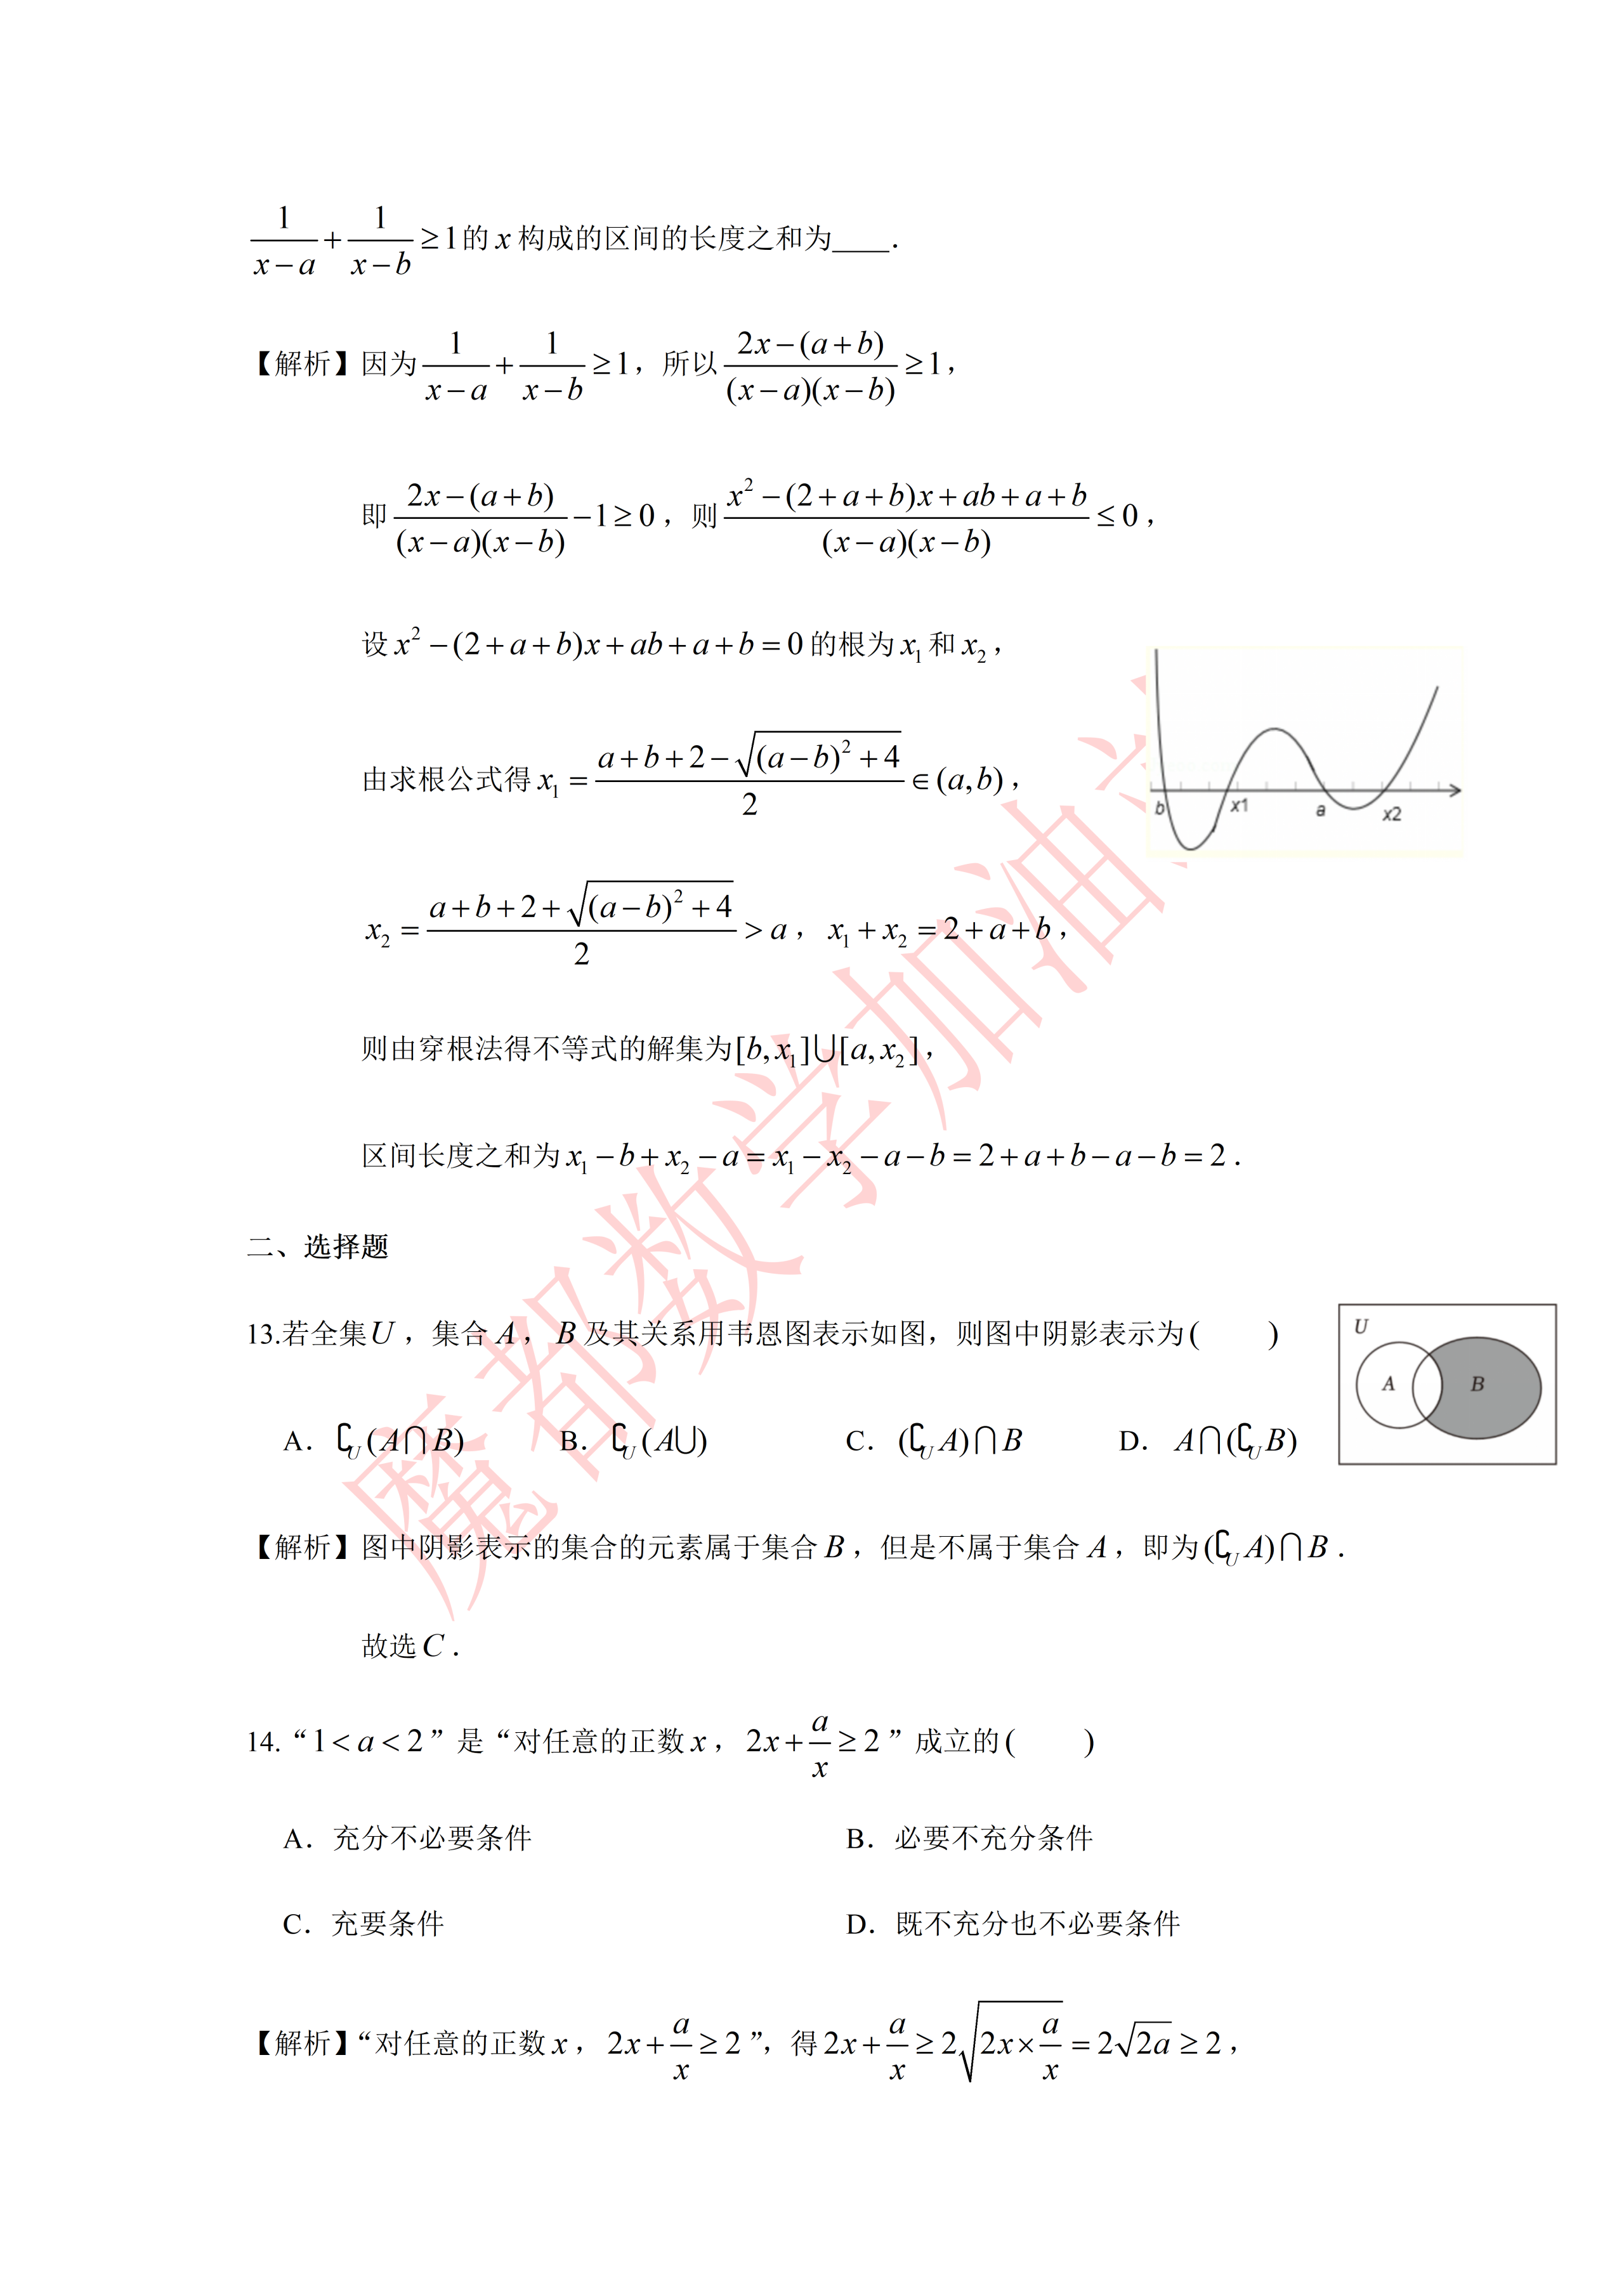
\includegraphics[width=.50\linewidth,trim=1786bp 2255bp 228bp 985bp,clip]{../原图/高一51_华师大二附中_国庆作业3/04.png}
\end{center}
\step{由求根公式得 $x_1=\dfrac{a+b+2-\sqrt{(a-b)^2+4}}{2}\in(a,b)$，}
\step{$x_2=\dfrac{a+b+2+\sqrt{(a-b)^2+4}}{2}>a$，$x_1+x_2=2+a+b$，}
\step{则由穿根法得不等式的解集为 $[b,x_1]\cup[a,x_2]$，}
% 原卷如此，照录未改（此处原卷作 $x_1-x_2$，按上一行 $x_1+x_2=2+a+b$ 当为 $x_1+x_2$）
\step{区间长度之和为 $x_1-b+x_2-a=x_1-x_2-a-b=2+a+b-a-b=2$.}
\solend

\fi

\end{enumerate}

\bigsec{二、选择题}

\begin{enumerate}
\setcounter{enumi}{12}

% 本题是“题干 + 图 + 选项”约 5.5cm 的一整块，图夹在题干与选项之间时 \keepwithprev 挡不住断点，
% 故按 高一30 第 13 题的成例在题前先量一次页高（守卫放在 \item 之前）。
\needvspace{6cm}
\item 若全集 $U$，集合 $A$、$B$ 及其关系用韦恩图表示如图，则图中阴影表示为\mbox{（\quad）}

\begin{center}
% 原卷该图印在题干与选项右侧（原图第 04 页），本稿移作居中排，直接裁取原图，不另存图片文件。
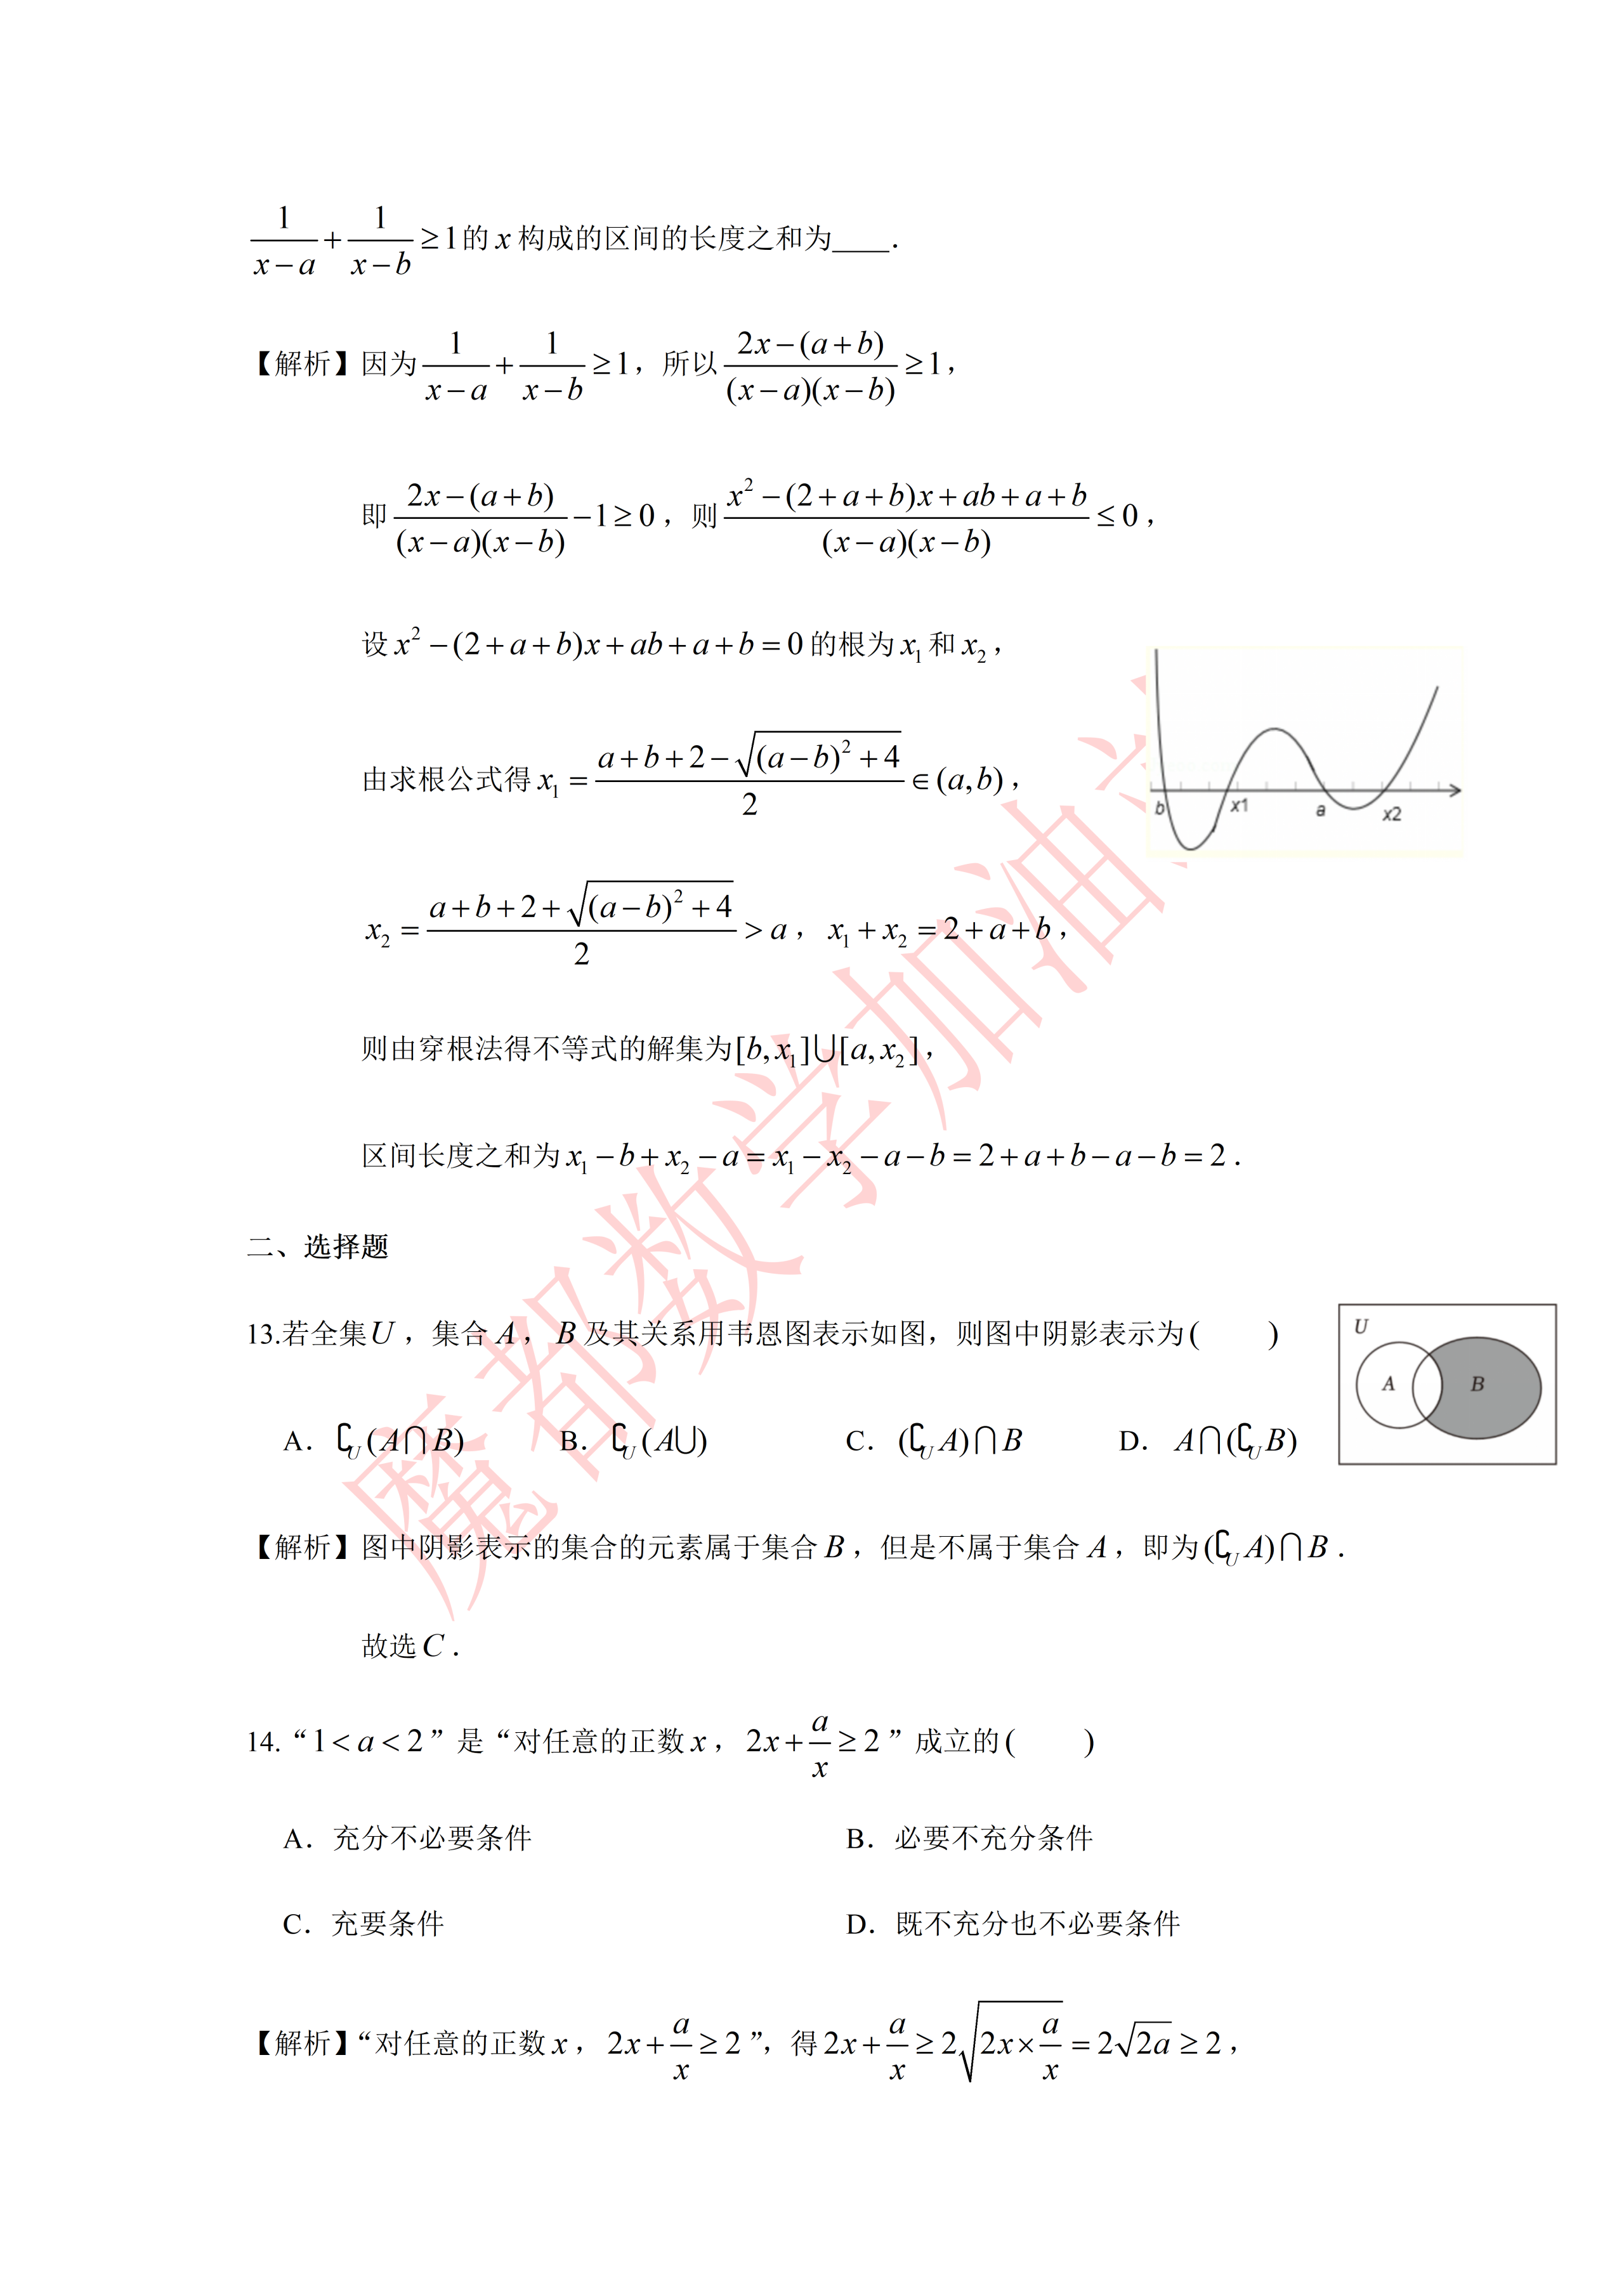
\includegraphics[width=.30\linewidth,trim=2105bp 1308bp 105bp 2050bp,clip]{../原图/高一51_华师大二附中_国庆作业3/04.png}
\end{center}

\keepwithprev
A. $\complement_U(A\cap B)$\qquad B. $\complement_U(A\cup B)$

C. $(\complement_U A)\cap B$\qquad D. $A\cap(\complement_U B)$

\ifanswer
\solbegin
\step{图中阴影表示的集合的元素属于集合 $B$，但是不属于集合 $A$，即为 $(\complement_U A)\cap B$.}
\step{故选 $C$.}
\solend

\fi

\item “$1<a<2$”是“对任意的正数 $x$，$2x+\dfrac ax\geqslant2$”成立的\mbox{（\quad）}

\keepwithprev
A. 充分不必要条件\qquad B. 必要不充分条件

C. 充要条件\qquad\qquad D. 既不充分也不必要条件

\ifanswer
\solbegin
\step{“对任意的正数 $x$，$2x+\dfrac ax\geqslant2$”，得 $2x+\dfrac ax\geqslant2\sqrt{2x\times\dfrac ax}=2\sqrt{2a}\geqslant2$，}
\step{所以 $\sqrt{2a}\geqslant1$，解得 $a\geqslant\dfrac12$，}
\step{若“$1<a<2$”得 $2x+\dfrac ax\geqslant2\sqrt{2x\times\dfrac ax}=2\sqrt{2a}>2\sqrt2>2$，}
\step{所以“$1<a<2$”$\Rightarrow$“对任意的正数 $x$，$2x+\dfrac ax\geqslant2$”，}
\step{所以“$1<a<2$”是“对任意的正数 $x$，$2x+\dfrac ax\geqslant2$”成立的充分不必要条件，}
\step{故选 $A$.}
\solend

\fi

\item 已知函数 $f(x)=2x-3$，$x\in(0,2)$，实数 $a$、$b$ 满足 $f(a)+f(b-1)=0$，则以下成立的有\mbox{（\quad）}

\keepwithprev
A. $a(b-1)$ 的最大值为 $\dfrac94$\qquad\qquad B. $b-\dfrac1a$ 的最大值为 $2$

C. $\dfrac1a+\dfrac1{4b}$ 的最小值为 $\dfrac9{16}$\qquad D. $-1<b-a<3$

\ifanswer
\solbegin
\step{因为函数 $f(x)=2x-3$，$x\in(0,2)$，实数 $a$、$b$ 满足 $f(a)+f(b-1)=0$，}
\step{所以 $2a-3+2(b-1)-3=0$，得 $a+b=4$，$a\in(0,2)$，$b\in(1,3)$，}
\step{所以 $a(b-1)=a(3-a)=-\left(a-\dfrac32\right)^2+\dfrac94$，$a\in(0,2)$，}
\step{所以 $0<a(b-1)\leqslant\dfrac94$，故选项 $A$ 正确；}
\step{$b-\dfrac1a=4-a-\dfrac1a=4-\left(a+\dfrac1a\right)\leqslant4-2=2$，}
\step{当且仅当 $a=1$，$b=3$ 时取等号，又 $b\in(1,3)$，故 $b-\dfrac1a<2$，故 $B$ 错误；}
\step{$\dfrac1a+\dfrac1{4b}=\dfrac14\left(\dfrac1a+\dfrac1{4b}\right)(a+b)=\dfrac14\left(1+\dfrac14+\dfrac ba+\dfrac a{4b}\right)=\dfrac5{16}+\dfrac14\left(\dfrac ba+\dfrac a{4b}\right)$}
\step{$\geqslant\dfrac5{16}+\dfrac14\cdot2\sqrt{\dfrac ba\cdot\dfrac a{4b}}=\dfrac9{16}$，当且仅当 $\dfrac ba=\dfrac a{4b}$，即 $a=2b=\dfrac83$ 时取等号，}
% 原卷如此，照录未改（“又 $a\in(0,2)$，”与下式之间原卷正文夹印“水印”二字）
\step{又 $a\in(0,2)$，水印 $\dfrac1a+\dfrac1{4b}<\dfrac9{16}$，故 $C$ 错误；}
\step{因为 $a\in(0,2)$，$b\in(1,3)$，所以 $-a\in(-2,0)$，所以 $b-a\in(-1,3)$，}
\step{故 $D$ 正确；}
\step{故选 $AD$.}
\solend

\fi

% 本题解析含图（“函数 f(x) 的图像如下”），图夹在解析行间，页末放不下会被拆开，
% 故在题前先量一次页高；上界取“题干 + 选项 + 图 + 首行解析”一块的高度。
\needvspace{6cm}
\item 设 $M_I$ 表示函数 $f(x)=|x^2-4x+2|$ 在闭区间 $I$ 上的最大值. 若正实数 $a$ 满足
$M_{[0,a]}\geqslant2M_{[a,2a]}$，则正实数 $a$ 的取值范围是\mbox{（\quad）}

\keepwithprev
A. $\left[2-\sqrt3,\dfrac12\right]$\qquad B. $[2-\sqrt3,1]$

C. $[2,2+\sqrt3]$\qquad\qquad D. $[2+\sqrt3,4]$

\ifanswer
\solbegin
\step{函数 $f(x)$ 的图像如下：}
\begin{center}
% 原卷该图印在解析行间（原图第 06 页），本稿直接裁取原图，不另存图片文件。
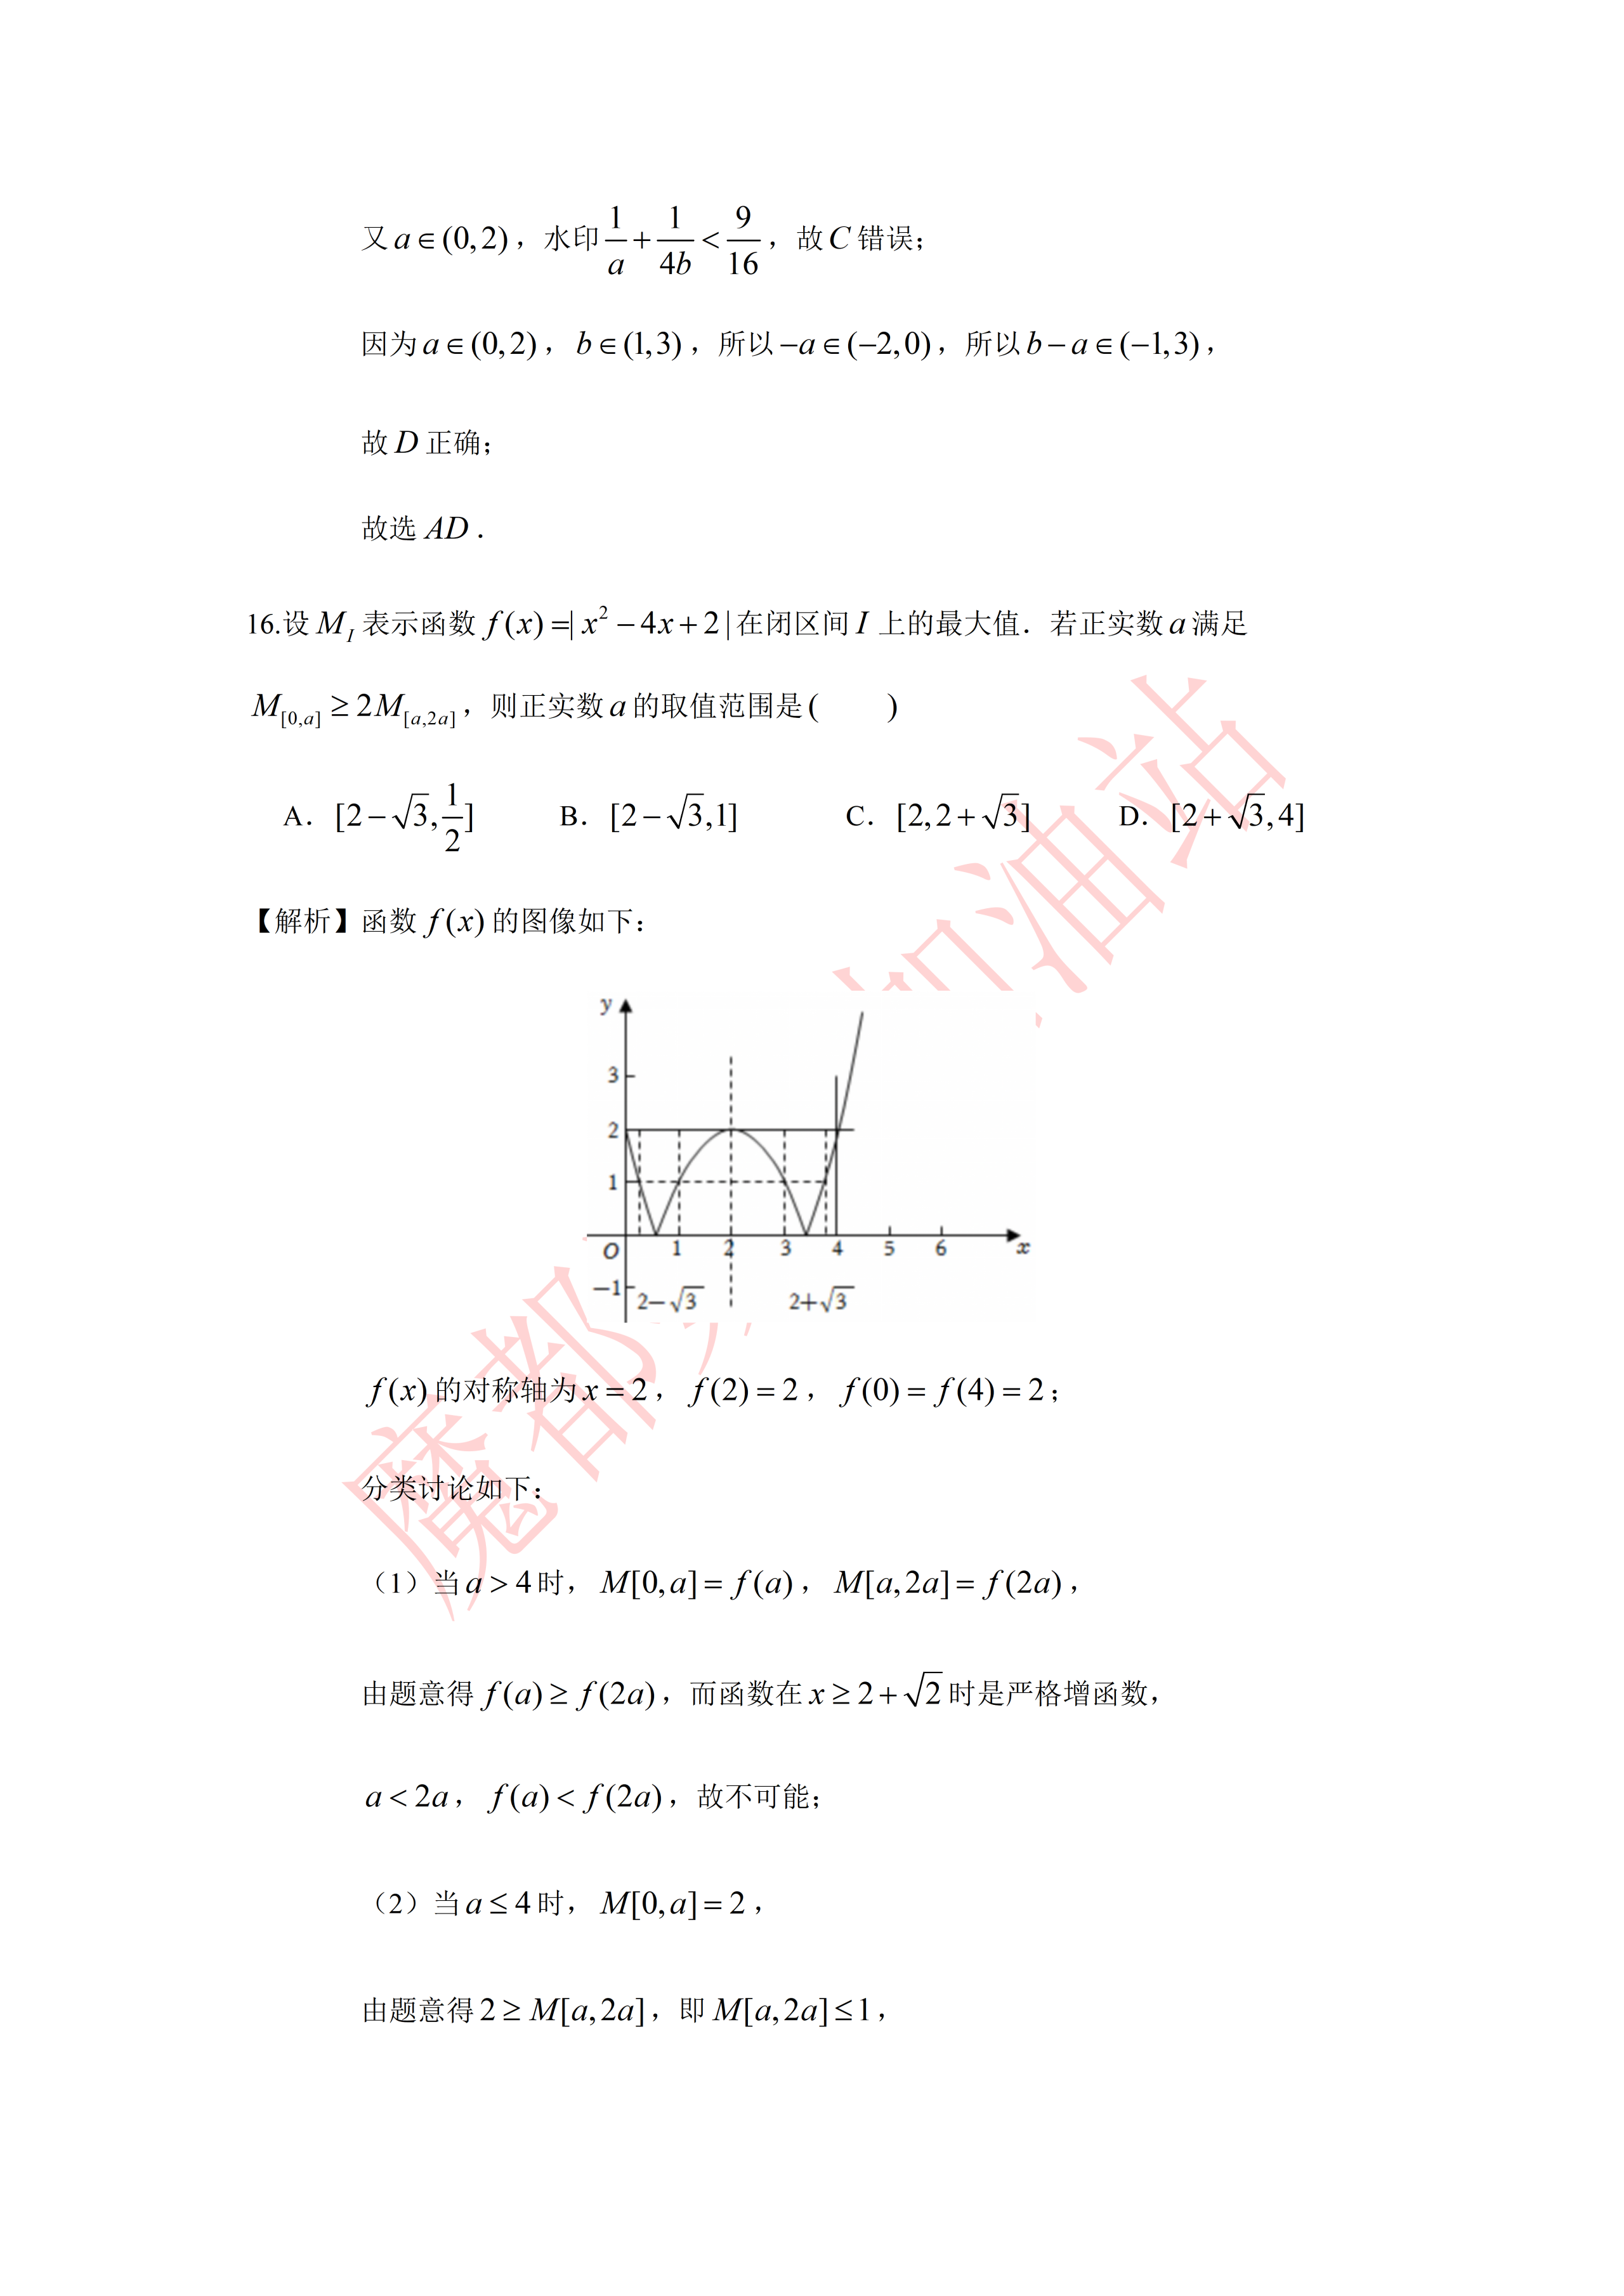
\includegraphics[width=.55\linewidth,trim=895bp 1535bp 915bp 1525bp,clip]{../原图/高一51_华师大二附中_国庆作业3/06.png}
\end{center}
\step{$f(x)$ 的对称轴为 $x=2$，$f(2)=2$，$f(0)=f(4)=2$；}
\step{分类讨论如下：}
\stepm{(1)}{当 $a>4$ 时，$M_{[0,a]}=f(a)$，$M_{[a,2a]}=f(2a)$，}
\step{由题意得 $f(a)\geqslant f(2a)$，而函数在 $x\geqslant2+\sqrt2$ 时是严格增函数，}
\step{$a<2a$，$f(a)<f(2a)$，故不可能；}
\stepm{(2)}{当 $a\leqslant4$ 时，$M_{[0,a]}=2$，}
\step{由题意得 $2\geqslant M_{[a,2a]}$，即 $M_{[a,2a]}\leqslant1$，}
\step{令 $f(x)=1$，解得 $x_1=2-\sqrt3$，$x_2=1$，$x_3=2+\sqrt3$，$x_4=3$，}
\step{则有 $a\geqslant2-\sqrt3$ 并且 $2a\leqslant1$，解得 $2-\sqrt3\leqslant a\leqslant\dfrac12$；}
\step{或者 $a\geqslant3$ 并且 $2a\leqslant2+\sqrt3$，无解；}
\step{故选 $A$.}
\solend

\fi

\end{enumerate}

\bigsec{三、解答题}

\begin{enumerate}
\setcounter{enumi}{16}

\item 已知 $M=\{x\mid2\leqslant x\leqslant5\}$，$N=\{x\mid a-1\leqslant x\leqslant2a+1\}$.
\begin{enumerate}[label=(\arabic*)]
\item 若 $M\subseteq N$，求实数 $a$ 的取值范围；
\item 若 $M\supseteq N$，求实数 $a$ 的取值范围.
\end{enumerate}

\ifanswer
\ans{（1）$[2,3]$；（2）$(-\infty,-2)$}
\fi

\ansspace[6]

\item 设集合 $A=\{x\mid|x+1|\leqslant3\}$，$B=\{x\mid0<x<3m\}$.
\begin{enumerate}[label=(\arabic*)]
\item 若 $A\cup B=A$，求实数 $m$ 的取值范围；
\item 设 $P=(\complement_R A)\cap B$，若 $\exists x\in\Z$ 且 $x\in P$，求实数 $m$ 的取值范围.
\end{enumerate}

\ifanswer
\solbegin
\stepm{(1)}{$A=\{x\mid|x+1|\leqslant3\}=\{x\mid-4\leqslant x\leqslant2\}$，且 $A\cup B=A$，所以 $B\subseteq A$.}
\step{若 $B=\varnothing$，此时 $0\geqslant3m$，解得 $m\leqslant0$；}
\step{若 $B\neq\varnothing$，此时 $0<3m$，且 $3m\leqslant2$，解得 $0<m\leqslant\dfrac23$；}
\step{则实数 $m$ 的取值范围是 $\left(-\infty,\dfrac23\right]$.}
\stepm{(2)}{因为 $\exists x\in\Z$ 且 $x\in P$，所以集合 $P$ 中至少存在一个整数.}
\step{$\complement_R A=\{x\mid x<-4\text{ 或 }x>2\}$，$B=\{x\mid0<x<3m\}$，}
\step{要使 $P=(\complement_R A)\cap B$ 中至少存在一个整数，则 $\begin{cases}3m>0\\3m>3\end{cases}$，解得 $m>1$，}
\step{则实数 $m$ 的取值范围是 $(1,+\infty)$.}
\solend

\fi

\ansspace[7]

\item 已知函数 $f(x)=x^2+(1-a)x-a(a\in\R)$.
\begin{enumerate}[label=(\arabic*)]
\item 解关于 $x$ 的不等式 $f(x)<0$；
\item 若 $\forall a\in[-1,1]$，$f(x)\geqslant0$ 恒成立，求实数 $x$ 的取值范围.
\end{enumerate}

\ifanswer
\solbegin
\stepm{(1)}{不等式 $x^2+(1-a)x-a<0$ 等价于 $(x-a)(x+1)<0$，}
\step{当 $a<-1$ 时，不等式的解集为 $(a,-1)$；}
\step{当 $a=-1$ 时，不等式的解集为 $\varnothing$；}
\step{当 $a>-1$ 时，不等式的解集为 $(-1,a)$.}
\stepm{(2)}{$x^2+(1-a)x-a=-a(x+1)+x^2+x$，}
\step{设 $g(a)=-a(x+1)+x^2+x$，$a\in[-1,1]$，}
\step{要使 $g(a)\geqslant0$ 在 $a\in[-1,1]$ 上恒成立，}
\step{只需 $\begin{cases}g(-1)\geqslant0\\g(1)\geqslant0\end{cases}$，即 $\begin{cases}x^2+2x+1\geqslant0\\x^2-1\geqslant0\end{cases}$，解得 $x\geqslant1$ 或 $x\leqslant-1$，}
\step{所以 $x$ 的取值范围为 $\{x\mid x\leqslant-1\text{ 或 }x\geqslant1\}$.}
\solend

\fi

\ansspace[7]

\item 若实数 $x$、$y$、$m$ 满足 $|x-m|>|y-m|$，则称 $x$ 比 $y$ 远离 $m$.
\begin{enumerate}[label=(\arabic*)]
\item 若 $2$ 比 $3x-4$ 远离 $1$，求 $x$ 的取值范围；
\item 设 $y=\dfrac{x+2}{x+1}$，其中 $x\in(0,\sqrt2)\cup(\sqrt2,+\infty)$，判断：$x$ 与 $y$ 哪一个更远离 $\sqrt2$？并说明理由.
\item 若 $x+y=2$，试问：$y$ 与 $x^2+y^2$ 哪一个更远离 $\dfrac12$？并说明理由.
\end{enumerate}

\ifanswer
\solbegin
\stepm{(1)}{由题意得 $|2-1|>|3x-4-1|$，所以 $|3x-5|<1$，解得 $\dfrac43<x<2$，}
\step{故 $x$ 的取值范围为 $\left(\dfrac43,2\right)$；}
\stepm{(2)}{$x$ 比 $y$ 更远离 $\sqrt2$，}
\step{理由如下：要证 $x$ 比 $y$ 更远离 $\sqrt2$，只要证 $|x-\sqrt2|>\left|\dfrac{x+2}{x+1}-\sqrt2\right|$，}
\step{即证 $|x-\sqrt2|>\left|\dfrac{(1-\sqrt2)(x-\sqrt2)}{x+1}\right|$，}
\step{因为 $x\in(0,\sqrt2)\cup(\sqrt2,+\infty)$，所以 $|x-\sqrt2|>0$，}
\step{所以只要证 $1>\dfrac{\sqrt2-1}{|x+1|}$，即证 $|x+1|>\sqrt2-1$，}
\step{因为 $x\in(0,\sqrt2)\cup(\sqrt2,+\infty)$，所以 $x+1\in(1,\sqrt2+1)\cup(\sqrt2+1,+\infty)$，}
\step{所以 $|x+1|>1>\sqrt2-1$，所以 $x$ 比 $y$ 更远离 $\sqrt2$；}
\stepm{(3)}{因为 $x^2+y^2\geqslant\dfrac{(x+y)^2}{2}=2$，当且仅当 $x=y=1$ 时等号成立，}
\step{所以 $\left|x^2+y^2-\dfrac12\right|=x^2+y^2-\dfrac12$，}
\step{从而 $\left|y-\dfrac12\right|-\left|x^2+y^2-\dfrac12\right|=\left|y-\dfrac12\right|-\left(x^2+y^2-\dfrac12\right)$，}
\step{①$y\geqslant\dfrac12$，$\left|y-\dfrac12\right|-\left|x^2+y^2-\dfrac12\right|=y-\dfrac12-\left(x^2+y^2-\dfrac12\right)=y-x^2-y^2$}
\step{$=y-(2-y)^2-y^2=-2y^2+5y-4=-2\left(y-\dfrac54\right)^2-\dfrac78<0$，}
\step{即 $\left|y-\dfrac12\right|<\left|x^2+y^2-\dfrac12\right|$；}
\step{②$y<\dfrac12$，}
\step{$\left|y-\dfrac12\right|-\left|x^2+y^2-\dfrac12\right|=\left(\dfrac12-y\right)-\left(x^2+y^2-\dfrac12\right)=-y-x^2-y^2+1$}
\step{$=-y-(2-y)^2-y^2+1=-2y^2+3y-3=-2\left(y-\dfrac34\right)^2-\dfrac{15}8<0$，}
\step{即 $\left|y-\dfrac12\right|<\left|x^2+y^2-\dfrac12\right|$；}
\step{综上，$\left|y-\dfrac12\right|<\left|x^2+y^2-\dfrac12\right|$，即 $x^2+y^2$ 比 $y$ 更远离 $\dfrac12$.}
\solend

\fi

\ansspace[9]

\item 对于非空有限整数集 $X$，$m\in\N^*$，定义 $X^m=\{x^m\mid x\in X\}$，对 $n\in\Z$，
$Y\oplus n=\{x+n\mid x\in Y\}$ 现有两个非空有限整数集 $A$、$B$，已知 $A\oplus1\subseteq B$ 且
$B^2\oplus(-4)\subseteq A$.
\begin{enumerate}[label=(\arabic*)]
\item 当 $A=\{-3,0\}$ 时求集合 $B$；
\item 证明：$A\subseteq\{-3,-2,0,1\}$；
\item 当 $A\oplus1=B$ 且 $B^2\oplus(-4)=A$ 时，任取 $a\in A$，$b\in B$ 构造函数
$f(x)=(x-a)(x-b)$ 问：当 $a$、$b$ 取何值时，$f(x)$ 的最小值最小？
\end{enumerate}

\ifanswer
\solbegin
\stepm{(1)}{因为 $A=\{-3,0\}$，$B^2\oplus(-4)\subseteq A$，}
\step{所以 $B^2\oplus(-4)$ 可能为 $\varnothing$、$\{-3\}$、$\{0\}$、$\{-3,0\}$，}
\step{当 $B^2\oplus(-4)=\varnothing$ 时 $B^2=\varnothing$，不满足非空，不合题意；}
\step{当 $B^2\oplus(-4)=\{-3\}$ 时 $B^2=\{1\}$，所以 $B=\{1,-1\}$、$\{1\}$、$\{-1\}$，}
\step{当 $B^2\oplus(-4)=\{0\}$ 时 $B^2=\{4\}$，所以 $B=\{2,-2\}$、$\{2\}$、$\{-2\}$，}
% 原卷如此，照录未改（此处作 $\{0,-3\}$，上一行同一集合作 $\{-3,0\}$）
\step{当 $B^2\oplus(-4)=\{0,-3\}$ 时 $B^2=\{4,1\}$，}
\step{所以 $B=\{1,2,-1,-2\}$、$\{2,-1,-2\}$、$\{2,1,-2\}$、$\{1,-1,-2\}$、$\{1,-1,2\}$、$\{1,2\}$、$\{-1,2\}$、$\{-1,-2\}$、$\{1,-2\}$，}
\step{又 $A\oplus1=\{-2,1\}\subseteq B$，得 $B$ 为 $\{1,-2\}$、$\{2,1,-2\}$、$\{1,-1,-2\}$、$\{1,2,-1,-2\}$.}
\stepm{(2)}{设 $x\in A$，因为 $A\oplus1\subseteq B$，所以 $x+1\in B$，}
\step{又 $B^2\oplus(-4)\subseteq A$，所以 $(x+1)^2-4\in A$，}
% 原卷如此，照录未改（此处及下文取 $x=2$ 处原卷均作 $(-4+1)^2-4=52-2a>0$）
\step{取 $x=-4$，则 $(-4+1)^2-4=52-2a>0$，$(5+1)^2-4=32\in A$，$\cdots$，}
\step{无限迭代，而 $A$ 为有限集，不合题意，舍去，即 $-4\notin A$；}
\step{取 $x=-3$，则 $(-3+1)^2-4=0\in A$，$(0+1)^2-4=-3\in A$，}
\step{得 $A$ 集合可为 $\{-3,0\}$；}
\step{取 $x=-2$，则 $(-2+1)^2-4=-3\in A$，$(-3+1)^2-4=0\in A$，}
\step{$(0+1)^2-4=-3\in A$，得 $A$ 集合可为 $\{-3,-2,0\}$；}
\step{取 $x=-1$，则 $(-1+1)^2-4=-4\in A$，又 $-4\notin A$，所以 $-1\notin A$，}
\step{取 $x=1$，则 $(1+1)^2-4=0\in A$，$(0+1)^2-4=-3\in A$，}
\step{$(-3+1)^2-4=0\in A$，得 $A$ 集合可为 $\{-3,0,1\}$，}
\step{取 $x=2$，则 $(2+1)^2-4=52-2a>0$，$(5+1)^2-4=32\in A$，$\cdots$，}
\step{无限迭代，而 $A$ 为有限集，不合题意，舍去，即 $2\notin A$，}
\step{同理当 $x<-4$ 或 $x>2$，且 $x\in\Z$ 时不符合 $A$ 为有限集，舍去；}
\step{故由上得 $A$ 集合可为 $\{-3,0\},\{-3,-2,0\},\{-3,0,1\},\{-3,-2,0,1\}$，}
\step{所以 $A\subseteq\{-3,-2,0,1\}$，}
\stepm{(3)}{当 $A\oplus1=B$ 且 $B^2\oplus(-4)=A$ 时，}
\step{设 $x\in B$，则 $x^2-4\in B^2\oplus(-4)=A$，}
% 原卷如此，照录未改（题设 $A=\{-3,0\}$，此处两个判别式取的是 $-2$ 与 $1$，均不属于 $A$）
\step{$x^2-4=-2$ 时 $x=\pm\sqrt2$，不为整数，不合题意；}
\step{$x^2-4=1$ 时 $x=\pm\sqrt5$，不为整数，不合题意；}
\step{所以 $A=\{-3,0\}$，又 $A\oplus1=B$，则 $B=\{-2,1\}$，}
\step{任取 $a\in A$，$b\in B$ 构造函数 $f(x)=(x-a)(x-b)$，}
\step{$f(x)=(x-a)(x-b)=x^2-(a+b)x+ab$}
\step{$=x^2-(a+b)x+\dfrac{(a+b)^2}{4}+ab-\dfrac{(a+b)^2}{4}$}
\step{$=\left[x-\dfrac{(a+b)}2\right]^2-\dfrac{(a-b)^2}{4}\geqslant-\dfrac{(a-b)^2}{4}$，所以 $f(x)_{min}=-\dfrac{(a-b)^2}{4}$，}
\step{又 $a\in A=\{-3,0\}$，$b\in B=\{-2,1\}$，所以 $a-b$ 的取值有 $-1,-4,2$，}
\step{所以 $f(x)_{min}=-\dfrac{(a-b)^2}{4}\geqslant-\dfrac{(-3-1)^2}{4}=-4$，}
\step{即当 $a=-3$，$b=1$ 时 $f(x)_{min}$ 的最小值为 $-4$.}
\solend

\fi

\ansspace*[12]

\end{enumerate}

\end{document}
